\RequirePackage{ifthen}
\newboolean{longpage}
\setboolean{longpage}{false}
\ifthenelse{\boolean{longpage}}%
{\documentclass[10pt]{article}}%
{\documentclass[10pt]{book}}

\newboolean{printlabelname}
\setboolean{printlabelname}{false}
\ifthenelse{\boolean{printlabelname}}{\usepackage[notref,notcite]{showkeys}}{}
\usepackage{pdfpages}


%% end detour
%\usepackage{amsmath}
\usepackage{xr}
\externaldocument{Math2565_ebook}

%%Page Size stuff

\newboolean{tabletsize}
\ifthenelse{\boolean{longpage}}% if longpage, tablet automatically false
{\setboolean{tabletsize}{false}}%% if not longpage, then set tablet
{\setboolean{tabletsize}{false}}

%% Layout for printed book through Amazon CreateSpace, perfect bound,
%% 8.5 x 11 paper size, 1in inner margin, 1/2in (roughly) outer margin

%% for regular sized pages
\ifthenelse{\boolean{longpage}}%
				{\usepackage[paperheight=20in,
				paperwidth=7in,%inner=1in,
				textheight=18in,textwidth=320pt%,marginparwidth=150pt,marginparsep=32pt
				]{geometry}}%
				%% else not long page; 
				{% not longpage
				\usepackage[paperheight=11in,paperwidth=8.5in,%
						inner=1in,textheight=9in,textwidth=320pt,marginparwidth=150pt,%
						marginparsep=32pt,bottom=1in,footskip=29pt]{geometry}}

\ifthenelse{\boolean{longpage}}%
{% longpage - do not make changes to the text height for exercises
\newcommand{\exercisegeometry}{%
\newgeometry{inner=72pt,outer=72pt,textheight=18in,%textwidth=320pt,
						marginparwidth=150pt,marginparsep=32pt}
															}
}% ends if longpage
{% not longpage - regular sized exercise sets
%%
%% the old size of exercises
%
%\newcommand{\exercisegeometry}{%
%\newgeometry{inner=72pt,%
						%outer=72pt,textheight=545pt,%textwidth=320pt,
						%marginparwidth=150pt,%
						%marginparsep=32pt,
						%}
															%}
%%
%% the new size of exercises
%%
\newcommand{\exercisegeometry}{%
\newgeometry{inner=72pt,%
						outer=72pt,textheight=9.25in,tmargin=.75in,%textwidth=320pt,
						marginparwidth=150pt,%
						marginparsep=32pt,footskip=29pt,
						%bottom=1in,
						}
															}
}% ends if/then/else longpage

\newcommand{\eendgeometry}{%
\newgeometry{inner=72pt,%
						outer=36pt,textheight=10in,%textwidth=320pt,
						marginparwidth=150pt,%
						marginparsep=32pt,
						%bottom=1in%,footskip=1.5in
						}%
													}

\newcommand{\prefacegeometry}{%
\newgeometry{inner=1in,textheight=9in,textwidth=320pt,marginparwidth=150pt,%
						marginparsep=32pt,bottom=1in,footskip=1.5in}
															}


\ifthenelse{\boolean{longpage}}{%
	\usepackage{everyshi}
	\textheight500cm
	\EveryShipout{%
	\pdfpagewidth=7in
	\pdfpageheight=\pagetotal
	\advance\pdfpageheight by 3in
	\advance\pdfpageheight by 2\topmargin
	\advance\pdfpageheight by \textheight
	\advance\pdfpageheight by -\pagegoal}
%%
	\newcounter{chapter}
	\newcommand{\chapter}{\refstepcounter{chapter}\Huge Chapter \thechapter \vskip 2\baselineskip\normalsize}
}{}


\usepackage{APEX_format}
%%%%
% Additional packages to support the book, not part of the APEX style.
%%%%
\usepackage{fancyhdr}
\usepackage{eso-pic}
\usepackage{lipsum}
\usepackage{units}
%\usepackage{pgfplots}
%\pgfplotsset{width=\marginparwidth+1pt,compat=1.3}
\usepackage[font=small]{caption}
%,justification=centering

%%%%
%% These are low level LaTeX commands that determine the 
%% look of the Chapter and Section headings.
%% Note the use in the chapter part of an external file
%% that contains graphics for each chapter start.
%%%%

%%%%
%% Commands for the header, utilizing the fancyhdr
%% (fancy header) package
%%%%

\pagestyle{fancy}
\fancyhead{}
%\fancyfoot{}
\renewcommand{\chaptermark}[1]{\markboth{\chaptername\ \thechapter\ \ \ \ {#1}}{}}
\renewcommand{\sectionmark}[1]{\markright{\thesection\ \ \ \  #1}}
\fancyhf{}         %Clears all header and footer fields, in preparation.
\renewcommand{\headrulewidth}{0pt}
\renewcommand{\footrulewidth}{0pt}

\ifthenelse{\boolean{longpage}}%
{}% end header of longpage
{% begin header/footer of not longpage
\fancyhfoffset[LE,RO]{\marginparwidth+\marginparsep}
%\fancyfoot[LE,RO]{\textbf{\thepage}} %Displays the page number in bold in the header,

\fancyfoot{}
\fancyfoot[LE]{\textbf{\thepage}}
\fancyfoot[RO]{\textbf{\thepage}}

%\fancyfoot[LE]{\begin{minipage}{\textwidth}%
%\noindent\hskip\marginparwidth\hskip\marginparsep\hskip-4pt\rule{\textwidth}{.4pt}
%\vskip.2\baselineskip
%\noindent\hskip\marginparwidth\hskip\marginparsep\hskip-4pt%
%Notes:
%\vskip 1.5in\textbf{\thepage}
%\end{minipage}} 

%\fancyfoot[RO]{\begin{minipage}{\textwidth+\marginparwidth+\marginparsep}%
%\rule{\textwidth-\marginparwidth-\marginparsep}{.4pt}
%\vskip.2\baselineskip
%Notes:
%\vskip 1.5in
%\hfill\textbf{\thepage}
%\end{minipage}}       


\fancyhead[LE]{\nouppercase{\leftmark}}
      %Displays the upper-level (chapter) information---
      % as determined above---in non-upper case in the header, 
      %to the right on even pages.
\fancyhead[RO]{\rightmark}
			%Displays the lower-level (section) information---as
      % determined above---in the header, to the left on odd pages.
      
}% End the ifthenelse{longpage}


\ifthenelse{\boolean{longpage}}% for changing the header
{% longpage
\newcommand{\exerciseheader}{}
\newcommand{\regularheader}{}
\newcommand{\endmatheader}{}
}% i.e, the above does nothing
{% now for a real change
\newcommand{\exerciseheader}{%
				\fancyhfoffset[LE,RO]{32pt}%
				\fancyfoot[LE]{\textbf{\thepage}}% 
				\fancyfoot[RO]{\textbf{\thepage}}
				\fancyhead{}% 
}

\newcommand{\regularheader}{%
\fancyhead[LE]{\nouppercase{\leftmark}}%
\fancyhead[RO]{\rightmark}%
%\fancyfoot[LE]{}
%\fancyfoot[RO]{}
\fancyfoot{}
\fancyfoot[LE]{\textbf{\thepage}}
\fancyfoot[RO]{\textbf{\thepage}}
%\fancyfoot[LE]{\begin{minipage}{\textwidth}%
%\noindent\hskip\marginparwidth\hskip\marginparsep\hskip-4pt\rule{\textwidth}{.4pt}
%\vskip.2\baselineskip
%\noindent\hskip\marginparwidth\hskip\marginparsep\hskip-4pt%
%Notes:
%\vskip 1.5in\textbf{\thepage}
%\end{minipage}} 

%\fancyfoot[RO]{\begin{minipage}{\textwidth+\marginparwidth+\marginparsep}%
%\rule{\textwidth-\marginparwidth-\marginparsep}{.4pt}
%\vskip.2\baselineskip
%Notes:
%\vskip 1.5in
%\hfill\textbf{\thepage}
%\end{minipage}}

\fancyhfoffset[LE,RO]{\marginparsep+\marginparwidth}
}

\newcommand{\qendheader}{%
		\fancyhead{}%
		\fancyfoot{}%
		}
}% ends if/then/else exercise/regular headers


%
%  Defining what the chapter titles look like
%

\newdimen\titleheight

\makeatletter
\def\@makechapterhead#1{%
  {\parindent \z@ \raggedright \reset@font
    {\Huge \thechapter: \scshape \textsc #1}
    \par\vskip 10\p@
    \hrule height 1pt
    \vskip 10\p@
  }}
%%  
%%%\makeatletter
%%\def\@makesectionhead#1{%
%%	 {\reset@font\LARGE\itshape\bfseries\strut #1 \thechapter.\thesection \ #1
%%	 }}

%%%%
%%
%%  For figures in the margin
%%
%%%%

%%\usepackage{wrapfig}
%%
%%\setlength{\marginparsep}{10pt}
%%\setlength{\wrapoverhang}{\marginparwidth}
%%\addtolength{\wrapoverhang}{\marginparsep}
%%
%%%\newenvironment{mfigure}[1]{%
%%%    \wrapfigure{#1}{0pt}%
%%%    \begin{minipage}{\marginparwidth}%
%%%    \centering%
%%%}{%
%%%    \end{minipage}%
%%%    \endwrapfigure%
%%%}


\ifthenelse{\boolean{longpage}}%
		{\newcommand{\mfigure}[5][]{%
		\vskip \baselineskip%
			\noindent\begin{minipage}{\textwidth}
  			\centering
  			\myincludegraphics{#5}
  			#1%
  			\captionsetup{type=figure}
	  		\caption{#3}\label{#4}
  		\end{minipage}
		}}
		{\newcommand{\mfigure}[5][]{%
		\ifthenelse{\isodd{\thepage}}%
			{\AddToShipoutPicture*{\put(427,\LenToUnit{#2\paperheight}){%
			\begin{minipage}{\marginparwidth}%
				\centering%
	  		\myincludegraphics[#1]{#5}%
  			\captionsetup{type=figure}%
  			%#1%
	  		\caption{#3}\label{#4}%
  		\end{minipage}}}}%
			{\AddToShipoutPicture*{\put(36,\LenToUnit{#2\paperheight}){%
			\begin{minipage}{\marginparwidth}%
			  \centering%
  			\myincludegraphics[#1]{#5}%
  			\captionsetup{type=figure}%
  			%#1%
	  		\caption{#3}\label{#4}%
  		\end{minipage}}}}%
		}}%

\ifthenelse{\boolean{longpage}}%
		{\newcommand{\mtable}[4]{
					\vskip \baselineskip%
					\noindent\begin{minipage}{\textwidth}
  					\centering\small
  					#4
  					\captionsetup{type=figure}
	  				\caption{#2}\label{#3}
  				\end{minipage}
  				\vskip\baselineskip}
  	}
		{\newcommand{\mtable}[4]{%
			\ifthenelse{\isodd{\thepage}}%
				{\AddToShipoutPicture*{\put(427,\LenToUnit{#1\paperheight}){%
					\begin{minipage}{\marginparwidth}%
  					\centering\small%
  					#4%
  					\captionsetup{type=figure}%
	  				\caption{#2}\label{#3}%
  				\end{minipage}}}}%
				{\AddToShipoutPicture*{\put(36,\LenToUnit{#1\paperheight}){%
					\begin{minipage}{\marginparwidth}%
 						 \centering\small%
 						 #4%
						  \captionsetup{type=figure}%
	  					\caption{#2}\label{#3}%
 					 \end{minipage}}}}%
		}}%

\ifthenelse{\boolean{longpage}}%
		{\newcommand{\mnote}[2]{%
					\hskip 25pt%
					\begin{minipage}{\marginparwidth}%
					\small%
					#2%
					\end{minipage}%
					\vskip\baselineskip%
		}%
		}%
		{\newcommand{\mnote}[2]{%
			\ifthenelse{\isodd{\thepage}}%
				{\AddToShipoutPicture*{\put(427,\LenToUnit{#1\paperheight}){%
					\begin{minipage}{\marginparwidth}
  					\small
  					#2
  				\end{minipage}}}}%
				{\AddToShipoutPicture*{\put(36,\LenToUnit{#1\paperheight}){%
					\begin{minipage}{\marginparwidth}
 						 \small
 						 #2
					\end{minipage}}}}
		}}

%\ifthenelse{\boolean{longpage}}%
		%{}
		%{\newcommand{\mfigurethree}[5][]{%
		%\ifthenelse{\isodd{\thepage}}%
			%{\AddToShipoutPicture*{\put(427,\LenToUnit{#2\paperheight}){%
			%\begin{minipage}{\marginparwidth}%
				%\centering%
	  		%\includemedia[#1]{\includegraphics{#5}}{#5.prc}%
  			%\captionsetup{type=figure}%
  			%%#1%
	  		%\caption{#3}\label{#4}%
  		%\end{minipage}}}}%
			%{\AddToShipoutPicture*{\put(36,\LenToUnit{#2\paperheight}){%
			%\begin{minipage}{\marginparwidth}%
			  %\centering%
  			%\includemedia[#1]{\includegraphics{#5}}{#5.prc}%
  			%\captionsetup{type=figure}%
  			%%#1%
	  		%\caption{#3}\label{#4}%
  		%\end{minipage}}}}%
		%}}%
		
		\newcommand{\mfigurethree}[6]{%
		\ifthenelse{\isodd{\thepage}}%
			{\AddToShipoutPicture*{\put(427,\LenToUnit{#3\paperheight}){%
			\begin{minipage}{\marginparwidth}%
				\centering%
				\ifthenelse{\boolean{in_threeD}}{% in 3D
	  		\includemedia[#1]{\includegraphics{#6_3D\colornamesuffix}}{#6_3D.prc}}%now not in 3D
				{\myincludegraphics[#2]{#6}}%
  			\captionsetup{type=figure}%
  			%#1%
	  		\caption{#4}\label{#5}%
  		\end{minipage}}}}%
			{\AddToShipoutPicture*{\put(36,\LenToUnit{#3\paperheight}){%
			\begin{minipage}{\marginparwidth}%
			  \centering%
  			\ifthenelse{\boolean{in_threeD}}{% in 3D
	  		\includemedia[#1]{\includegraphics{#6_3D\colornamesuffix}}{#6_3D.prc}}%now not in 3D
				{\myincludegraphics[#2]{#6}}%
  			\captionsetup{type=figure}%
  			%#1%
	  		\caption{#4}\label{#5}%
  		\end{minipage}}}}%
		}

%\AddToShipoutPicture{\ifthenelse{\ifodd{\thepage}}%
%{\put(10,10){\begin{tikzpicture}\draw (0,0) circle (5pt);\end{tikzpicture}}}%
%{\put(100,100){\begin{tikzpicture}\draw (0,0) circle (5pt);\end{tikzpicture}}}}%
%

%\AddToShipoutPictureBG{%
% \AtPageLowerLeft{\hspace{1cm}A small logo: \rule{2cm}{3cm}}}
% 
%}{\AddToShipoutPicture*{\put(36,\LenToUnit{#2\paperheight})}}%
%{%
%\begin{minipage}{\marginparwidth}
%  \centering
%  \includegraphics{#1}
%  \captionof{figure}{#3}
%  \end{minipage}}}
%\AddToShipoutPicture*{\put(\LenToUnit{.5\paperwidth},\LenToUnit{.75\paperheight}){%
%  \begin{minipage}{100pt}
%  \centering
%  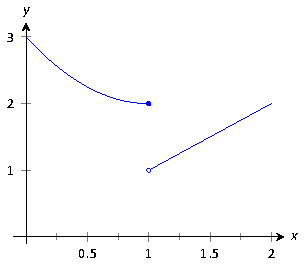
\includegraphics{test-figure2.pdf}
%  \captionof{figure}{Test caption}
%  \end{minipage}}}


%\newenvironment{mfigurefile}[2]{%
%\begin{tikzpicture}[remember picture,overlay]%
%\ifthenelse{\isodd{\thepage}}{\node [xshift=-36pt-.5\marginparwidth,yshift=#2\paperheight] at (current page.south east) }{\node [xshift=36pt+.5\marginparwidth,yshift=#2\paperheight] at (current page.south west) }%
%{\input{#1}};}%
%{\end{tikzpicture}%
%}

%\DeclareCaptionType{mytype}[Typename][List of mytype]


    
%%%%
%% End margin figure 
%%%%    
    

\newcommand{\bmx}[1]{\left[\hskip -3pt\begin{array}{#1} }
\newcommand{\emx}{\end{array}\hskip -3pt\right]}

\newcommand{\btz}{\begin{center}\begin{tikzpicture}}
\newcommand{\etz}{\end{tikzpicture}\end{center}}

\newcommand{\ds}{\displaystyle}

\newcommand{\fp}{\ensuremath{f\,'}}
\newcommand{\fpp}{\ensuremath{f\,''}}

\newcommand{\Fp}{\ensuremath{F\primeskip'}}
\newcommand{\Fpp}{\ensuremath{F\primeskip''}}

\newcommand{\yp}{\ensuremath{y\primeskip'}}
\newcommand{\gp}{\ensuremath{g\primeskip'}}

\newcommand{\dx}{\ensuremath{\Delta x}}
\newcommand{\dy}{\ensuremath{\Delta y}}
%\newcommand{\dz}{\ensuremath{\Delta z}}
\newcommand{\ddz}{\ensuremath{\Delta z}}

\newcommand{\thet}{\ensuremath{\theta}}
\newcommand{\norm}[1]{\ensuremath{||\ #1\ ||}}
\newcommand{\vnorm}[1]{\ensuremath{\norm{\vec #1}}}
\newcommand{\snorm}[1]{\ensuremath{\left|\left|\ #1\ \right|\right|}}
\newcommand{\la}{\left\langle}
\newcommand{\ra}{\right\rangle}
\newcommand{\dotp}[2]{\ensuremath{\vec #1 \cdot \vec #2}}
\newcommand{\proj}[2]{\ensuremath{\text{proj}_{\,\vec #2}{\,\vec #1}}}
\newcommand{\crossp}[2]{\ensuremath{\vec #1 \times \vec #2}}
\newcommand{\veci}{\ensuremath{\vec i}}
\newcommand{\vecj}{\ensuremath{\vec j}}
\newcommand{\veck}{\ensuremath{\vec k}}
\newcommand{\vecu}{\ensuremath{\vec u}}
\newcommand{\vecv}{\ensuremath{\vec v}}
\newcommand{\vecw}{\ensuremath{\vec w}}
\newcommand{\vecx}{\ensuremath{\vec x}}
\newcommand{\vecy}{\ensuremath{\vec y}}
\newcommand{\vrp}{\ensuremath{\vec r\, '}}
\newcommand{\vsp}{\ensuremath{\vec s\, '}}
\newcommand{\vrt}{\ensuremath{\vec r(t)}}
\newcommand{\vst}{\ensuremath{\vec s(t)}}
\newcommand{\vvt}{\ensuremath{\vec v(t)}}
\newcommand{\vat}{\ensuremath{\vec a(t)}}
\newcommand{\px}{\ensuremath{\partial x}}
\newcommand{\py}{\ensuremath{\partial y}}
\newcommand{\pz}{\ensuremath{\partial z}}
\newcommand{\pf}{\ensuremath{\partial f}}
\newcommand{\underlinespace}{\underline{\phantom{xxxxxx}}}

\newcommand{\mathN}{\ensuremath{\mathbb{N}}}

\newcommand{\zerooverzero}{\ensuremath{\ds \raisebox{8pt}{\text{``\ }}\frac{0}{0}\raisebox{8pt}{\text{\ ''}}}}


\newcommand{\myrule}{\rule[-4pt]{0pt}{13pt}}
\newcommand{\mmrule}{\rule[-10pt]{0pt}{15pt}}
\newcommand{\myds}{\ds\mmrule}
\newcommand{\deriv}[2]{\ensuremath{\myds\frac{d}{dx}\left(#1\right)=#2}}
\newcommand{\myint}[2]{\ensuremath{\myds\int #1\ dx=} \ensuremath{\ds #2}}

\DeclareMathOperator{\sech}{sech}
\DeclareMathOperator{\csch}{csch}

\newcommand{\sword}[1]{\textbf{#1}}

\newcommand{\primeskip}{\hskip.75pt}

%%%% Begin Header TikZ

%  Some TiKZ  shortcuts to help make drawing 3D vectors faster.
%

\newcommand{\plotlinecolor}{blue}

%
% Draw x and y tick marks
%
\newcommand{\drawxticks}[1]
{\foreach \x in {#1}
		{\draw  (\x,-.1)--(\x,.1);
			};
}
\newcommand{\drawyticks}[1]
{\foreach \x in {#1}
		{\draw  (-.1,\x)--(.1,\x);
			};
}

\newcommand{\drawxlines}[3]
{\draw[<->] (#1,0) -- (#2,0) node [right] {$x$};
\foreach \x in {#3}
		{\draw  (\x,-.1)--(\x,.1);
			};
}

\newcommand{\drawylines}[3]
{\draw[<->] (0,#1) -- (0,#2) node [above] {$y$};
\foreach \x in {#3}
		{\draw  (-.1,\x)--(.1,\x);
			};
}

\newcommand{\drawxlabels}[1]
{\foreach \x in {#1}
		{\draw  (\x,-.1) node [below] {\scriptsize $\x$};
		};
}

\newcommand{\drawylabels}[1]
{\foreach \x in {#1}
		{\draw  (-.1,\x) node [left] {\scriptsize $\x$};
		};
}

%% draw a box of margin width size to see if figure is properly contained within
\newcommand{\marginsizebox}{\draw (0,0)--(\marginparwidth,0)--(\marginparwidth,3)--(0,3)--cycle;}

%%%%
%%%%

\newcommand{\asyouread}[1]{\begin{tikzpicture}
\ifthenelse{\boolean{in_color}}{\node [preaction={fill=black,opacity=.5,transform canvas={xshift=1mm,yshift=-1mm}}, right color=blue!80!black!30, left color=blue!80] at (0,0) {\textcolor{white}{\textsf{\textit{AS YOU READ $\ldots$}}}};}
{\node [preaction={fill=black,opacity=.5,transform canvas={xshift=1mm,yshift=-1mm}}, right color=black!30, left color=black!10] at (0,0) {\textcolor{white}{\textsf{\textit{AS YOU READ $\ldots$}}}};}
\end{tikzpicture}
\begin{enumerate}
#1
\end{enumerate}
\vskip 20pt}

%%%%
%%  A new figure environment, trying to fix the float problem.
%%
%%%%

\newcounter{myfigurecounter}[chapter]
\renewcommand\themyfigurecounter{\thechapter.\arabic{myfigurecounter}}
\newenvironment{myfigure}{\refstepcounter{myfigurecounter}}{}
\newcommand{\mycaption}[1]{%
\begin{center}%
\vskip -1.5\baselineskip
\begin{tikzpicture}%
\draw (0,0) node [text width=\textwidth,align=center] {Figure \themyfigurecounter: #1};%
\end{tikzpicture}%
\end{center}%
}
\usepackage{pgfplots}
\pgfplotsset{compat=1.8}
\usepackage{pdfpages,refcount}


\ifthenelse{\boolean{xetex}}%
	{\sffamily
	%%\usepackage{fontspec}
	\usepackage{mathspec}
	\setallmainfonts[Mapping=tex-text]{Calibri}
	\setmainfont[Mapping=tex-text]{Calibri}
	\setsansfont[Mapping=tex-text]{Calibri}
	\setmathsfont(Greek){[cmmi10]}}
	{\usepackage[sfdefault,lf]{carlito}
	%% The 'lf' option for lining figures
	%% The 'sfdefault' option to make the base font sans serif
	\usepackage[T1]{fontenc}
	\renewcommand*\oldstylenums[1]{\carlitoOsF #1}}
	
	\ifthenelse{\boolean{luatex}}%
	{\sffamily
	\usepackage{fontspec}
	\usepackage{unicode-math}
	\usepackage{mathspec}
	\setallmainfonts[Mapping=tex-text]{Calibri}
	\setmainfont{Calibri}
	\setsansfont[Mapping=tex-text]{Calibri}
	\setmathfont[range=\mathup]{Calibri}
	\setmathfont[range=\mathit]{Calibri Italic}
	}
	{}

\makeindex

%%%\tracingonline=1
\begin{document}
%\printexercisenames
\printincolor
%\printinblackandwhite
%\printallanswers


%
%%%%%%%%%%
%%%
%%%  Set criteria for the format of the book.
%%%  This supercedes anything set in the Text_Header.
%%%
%%%%%%%%%%



%\printinblackandwhite

%\printexercisenames

%\nodrawexamplelines

%\printallanswers


\normalem



%%%\pagenumbering{roman}

%%%%%%
%%%		For editing purposes, block comment down to 
%%%		the next mark
%%%%%%

%%%%\input{cover/front_cover_in_text}
%%%%\clearpage
%%%%\thispagestyle{empty}
\frontmatter
%%%%
%%%%\title{\textsc{Fundamentals of Matrix Algebra}\\
%%%%{\small Version 2.1011}}
%%%%\author{Gregory N. Hartman, Ph.D.}
%%%%\date{}

\vspace*{\stretch{.5}}

\hskip 125pt\begin{minipage}{\textwidth}
\begin{flushright}

\textsc{{\Huge Math 1565 Accelerated Calculus I}} \\


\textsl{\large Fall 2018 Edition}, 
{\large University of Lethbridge}\\

{An adaptation of the \apex\ Calculus textbook, edited by Sean Fitzpatrick}

\bigskip

\Large
\vspace{1in}

Gregory Hartman, Ph.D.

\emph{\small Department of Applied Mathematics}

\emph{\small Virginia Military Institute}\vskip15pt

\parbox{200pt}{\textit{Contributing Authors}}\hskip 2cm \phantom{.}

Troy Siemers, Ph.D.

\emph{\small Department of Applied Mathematics}

\emph{\small Virginia Military Institute}\vskip 15pt

Brian Heinold, Ph.D.

\emph{\small Department of Mathematics and Computer Science}

\emph{\small Mount Saint Mary's University}\vskip 15pt

Dimplekumar Chalishajar, Ph.D.

\emph{\small Department of Applied Mathematics}

\emph{\small Virginia Military Institute}\vskip 25pt

\parbox{200pt}{\textit{Editor}}\hskip 2cm \phantom{.}
%\textit{Editor}\hskip 7cm\phantom{.}

Jennifer Bowen, Ph.D.

\emph{\small Department of Mathematics and Computer Science}

\emph{\small The College of Wooster}

\normalsize
\end{flushright}
\end{minipage}

\vspace{\stretch{1}}


\thispagestyle{empty}
\clearpage

\vspace*{\stretch{5}}
\noindent\hskip -1in\begin{minipage}{2in}
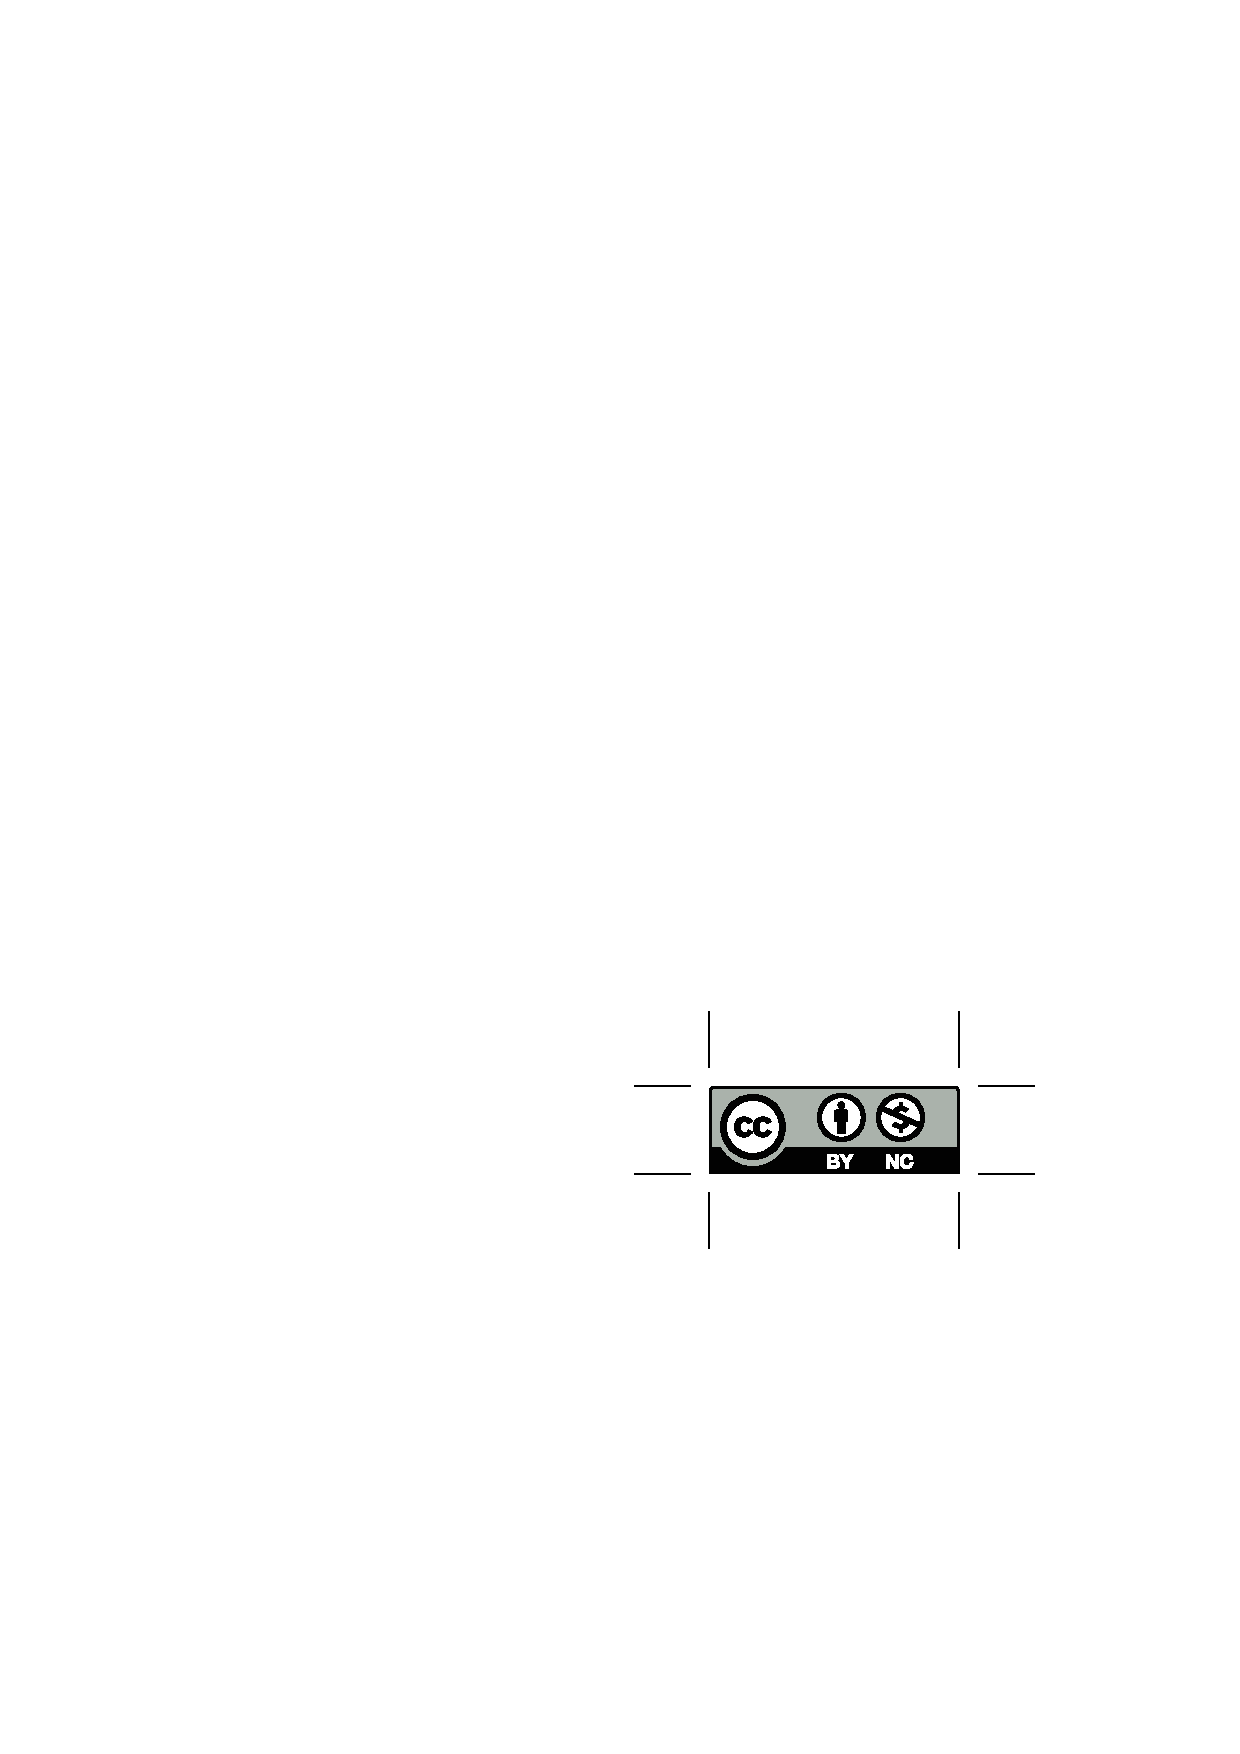
\includegraphics{text/by-nc} 
\end{minipage}
\begin{minipage}{3in}
\noindent Copyright \copyright\ 2018 Gregory Hartman

Licensed to the public under Creative Commons Attribution-Noncommercial 4.0 International Public License
\end{minipage}

\bigskip

\bigskip



\bigskip

\begin{minipage}{3.3in}
This version of the text was assembled and edited by Sean Fitzpatrick, University of Lethbridge, November 2015, revised most recently in May 2018. 

This work is licensed under the Creative Commons Attribution-Noncommercial-ShareAlike 4.0 International Public License
\end{minipage}
\vspace{\stretch{1}} 
\thispagestyle{empty}
\clearpage
%
%
%\cleardoublepage
%%%%\phantomsection
%%%%\input{text/thanks}
%%%%\addcontentsline{toc}{chapter}{Thanks} 
%%%%\clearpage{\pagestyle{empty}\cleardoublepage}
%%%%\phantomsection
%%%%\thispagestyle{empty}
\Huge
\noindent {\bf \textsc{Preface}}\\
\large
\emph{A Note on Using this Text}
\vspace{1in}
\normalsize

Thank you for reading this short preface. Allow us to share a few key points about the text so that you may better understand what you will find beyond this page.

This text comprises a three--volume series on Calculus. The first part covers material taught in many ``Calc 1'' courses: limits, derivatives, and the basics of integration, found in Chapters 1 through 6.1. The second text covers material often taught in ``Calc 2:'' integration and its applications, along with an introduction to sequences, series and Taylor Polynomials, found in Chapters 5 through 8. The third text covers topics common in ``Calc 3'' or ``multivariable calc:'' parametric equations, polar coordinates, vector--valued functions, and functions of more than one variable, found in Chapters 9 through 13. All three are available separately for free at \texttt{\href{http://apexcalculus.com}{www.apexcalculus.com}}. %These three texts are intended to work together and make one cohesive text, \textit{APEX Calculus}, which can also be downloaded from the website. 

Printing the entire text as one volume makes for a large, heavy, cumbersome book. One can certainly only print the pages they currently need, but some prefer to have a nice, bound copy of the text. Therefore this text has been split into these three manageable parts, each of which can be purchased for under \$15 at \href{http://amazon.com}{Amazon.com}.\\ 



%A result of this splitting is that sometimes a concept is said to be explored in a ``later section,'' though that section does not actually appear in this particular text. Downloading the .pdf of \textit{APEX Calculus} will ensure that you have all the content.  
%material is referenced that is not contained in the present text. The context should make it clear whether the ``missing'' material is in the \textit{Calculus I} or \textit{Calculus III} portion. Downloading the appropriate .pdf, or the whole \textit{APEX Calculus} .pdf, will give access to these topics.
% This splitting of the material also results in unfortunate page/chapter numberings. Chapter 5 of this text is Chapter 1 of \textit{Calculus II}. Apart from these numberings, page--for--page the content of the sections that appear in both \textit{Calculus I} and \textit{Calculus II} are identical.\\ %For instance, in this text, ``Theorem 20'' may be mentioned, although Theorem 20 is only presented in Part I. To minimize confusion, theorems, definitions and key ideas are referenced by their title or subject matter, not their number.

%The current publisher of this text does not allow one text to be split across multiple volumes, with continuity of chapters and page numberings. This is the one drawback of the current publishing model that has many advantages, highlighted below. Because of this, there are a few peculiarities 

\noindent\textbf{\large For Students: How to Read this Text}\\

Mathematics textbooks have a reputation for being hard to read. High--level mathematical writing often seeks to say much with few words, and this style often seeps into texts of lower--level topics. This book was written with the goal of being easier to read than many other calculus textbooks, without becoming too verbose. 

Each chapter and section starts with an introduction of the coming material, hopefully setting the stage for ``why you should care,'' and ends with a look ahead to see how the just--learned material helps address future problems. 

\textit{Please read the text;} it is written to explain the concepts of Calculus. There are numerous examples to demonstrate the meaning of definitions, the truth of theorems, and the application of mathematical techniques. When you encounter a sentence you don't understand, read it again. If it still doesn't make sense, read on anyway, as sometimes confusing sentences are explained by later sentences.

\textit{You don't have to read every equation.} The examples generally show ``all'' the steps needed to solve a problem. Sometimes reading through each step is helpful; sometimes it is confusing. When the steps are illustrating a new technique, one probably should follow each step closely to learn the new technique. When the steps are showing the mathematics needed to find a number to be used later, one can usually skip ahead and see how that number is being used, instead of getting bogged down in reading how the number was found.

\textit{Most proofs have been omitted.} In mathematics, \textit{proving} something is always true is extremely important, and entails much more than testing to see if it works twice. However, students often are confused by the details of a proof, or become concerned that they should have been able to construct this proof on their own. To alleviate this potential problem, we do not include the proofs to most theorems in the text. The interested reader is highly encouraged to find proofs online or from their instructor. In most cases, one is very capable of understanding what a theorem \textit{means} and \textit{how to apply it} without knowing fully \textit{why} it is true.
\\

\thispagestyle{empty}
\noindent\textbf{\large Interactive, 3D Graphics}\\

New to Version 3.0 is the addition of interactive, 3D graphics in the .pdf version. Nearly all graphs of objects in space can be rotated, shifted, and zoomed in/out so the reader can better understand the object illustrated. 

As of this writing, the only pdf viewers that support these 3D graphics are Adobe Reader \& Acrobat (and only the versions for PC/Mac/Unix/Linux computers, not tablets or smartphones). To activate the interactive mode, click on the image. Once activated, one can click/drag to rotate the object and use the scroll wheel on a mouse to zoom in/out. (A great way to investigate an image is to first zoom in on the page of the pdf viewer so the graphic itself takes up much of the screen, then zoom inside the graphic itself.) A CTRL-click/drag pans the object left/right or up/down. By right-clicking on the graph one can access a menu of other options, such as changing the lighting scheme or perspective. One can also revert the graph back to its default view. If you wish to deactive the interactivity, one can right-click and choose the ``Disable Content'' option. \\

\noindent\textbf{\large Thanks}\\

There are many people who deserve recognition for the important role they have played in the development of this text. First, I thank Michelle for her support and encouragement, even as this ``project from work'' occupied my time and attention at home. Many thanks to Troy Siemers, whose most important contributions extend far beyond the sections he wrote or the 227 figures he coded in Asymptote for 3D interaction.  He provided incredible support, advice and encouragement for which I am very grateful. My thanks to Brian Heinold and Dimplekumar Chalishajar for their contributions and to Jennifer Bowen for reading through so much material and providing great feedback early on. Thanks to Troy, Lee Dewald, Dan Joseph, Meagan Herald, Bill Lowe, John David, Vonda Walsh, Geoff Cox, Jessica Libertini and other faculty of VMI who have given me numerous suggestions and corrections based on their experience with teaching from the text. (Special thanks to Troy, Lee \& Dan for their patience in teaching Calc III while I was still writing the Calc III material.) Thanks to Randy Cone for encouraging his tutors of VMI's Open Math Lab to read through the text and check the solutions, and thanks to the tutors for spending their time doing so. A very special thanks to Kristi Brown and Paul Janiczek who took this opportunity far above \& beyond what I expected, meticulously checking every solution and carefully reading every example. Their comments have been extraordinarily helpful. I am also thankful for the support provided by Wane Schneiter, who as my Dean provided me with extra time to work on this project. I am blessed to have so many people give of their time to make this book better.\\

\noindent\textbf{\large \apex\  -- Affordable Print and Electronic teXts}\\

\apex\ is a consortium of authors  who collaborate to produce high--quality, low--cost textbooks. The current textbook--writing paradigm is facing a potential revolution as desktop publishing and electronic formats increase in popularity. However, writing a good textbook is no easy task, as the time requirements alone are substantial. It takes countless hours of work to produce text, write examples and exercises, edit and publish. Through collaboration, however, the cost to any individual can be lessened, allowing us to create texts that we freely distribute electronically and sell in printed form for an incredibly low cost. Having said that, nothing is entirely free; someone always bears some cost. This text ``cost'' the authors of this book their time, and that was not enough. \textit{APEX Calculus} would not exist had not the Virginia Military Institute, through a generous Jackson--Hope grant, given the lead author significant time away from teaching so he could focus on this text.

Each text is available as a free .pdf, protected by a Creative Commons Attribution - Noncommercial 4.0 copyright. That  means you can give the .pdf to anyone you like, print it in any form you like, and even edit the original content and redistribute it. If you do the latter, you must  clearly reference this work and you cannot sell your edited work for money.

We encourage others to adapt this work to fit their own needs. One might add sections that are ``missing'' or remove sections that your students won't need. The source files can be found at \texttt{\href{https://github.com/APEXCalculus}{github.com/APEXCalculus}}.

You can learn more at \texttt{\href{http://www.vmi.edu/APEX}{www.vmi.edu/APEX}}.
\thispagestyle{empty}


%%%%\addcontentsline{toc}{chapter}{Preface}
%%%%\clearpage{\pagestyle{empty}\cleardoublepage}
%%%%\phantomsection
%
% The following is the correct TOC; the 
%
%%%%

\addtocontents{toc}{\protect\thispagestyle{empty}}
\addcontentsline{toc}{chapter}{Table of Contents}
\tableofcontents
\clearpage{\pagestyle{empty}\cleardoublepage}

\phantomsection
\prefacegeometry
\addcontentsline{toc}{chapter}{Preface}
\thispagestyle{empty}
\Huge
\noindent {\bf \textsc{Preface}}\\
\normalsize

This document is an attempt to provide a custom textbook that covers the entire curriculum (as of September 2017) for the course Math 1565 (Accelerated Calculus I) at the University of Lethbridge at minimal cost to the student.


Most of this textbook is adapted from the \textit{APEX Calculus} textbook project, which originated in the Department of Applied Mathematics at the Virginia Military Institute. (See \href{http://www.apexcalculus.com}{apexcalculus.com}.) On the following page you'll find the original preface from their text, which explains their project in more detail. They have produced calculus textbook that is \textbf{free} in two regards: it's free to you, the student, in the sense that you can download the PDF from their website at no cost, and do with it as you wish (share it, print it, etc.) It's also free in the sense of being an \textit{open source} textbook: the authors have made all the files needed to produce the textbook freely available, and allow others (such as myself) to edit the text to suit the needs of various courses (such as Math 1560).

What's even better is that the textbook is of remarkably high production quality: unlike many free texts, it is polished and professionally produced, with graphics on almost every page, and a large collection of exercises (with selected answers!). 

I hope that you find this textbook useful. If you find any errors, or if you have any suggestions as to how the material could be better arranged or presented, please let me know. (The beauty of the open source textbook is that it can be edited at any time!) In particular, if you find a particular topic that you think needs further explanation, or more examples, or more exercises, please let us know. My hope is that this text will be improved every time it is used for this course.

\vspace{1in}

\begin{flushright}
Sean Fitzpatrick\\
Department of Mathematics and Computer Science\\
University of Lethbridge\\
April, 2017
\end{flushright}

\newpage

\Huge
\noindent {\bf \textsc{Preface to APEX Calculus}}\\
\large
\emph{A Note on Using this Text}
\vskip2\baselineskip
\normalsize

Thank you for reading this short preface. Allow us to share a few key points about the text so that you may better understand what you will find beyond this page.

This text is Part I of a three--text series on Calculus. The first part covers material taught in many ``Calc 1'' courses: limits, derivatives, and the basics of integration, found in Chapters 1 through 6.1. The second text covers material often taught in ``Calc 2:'' integration and its applications, along with an introduction to sequences, series and Taylor Polynomials, found in Chapters 5 through 8. The third text covers topics common in ``Calc 3'' or ``multivariable calc:'' parametric equations, polar coordinates, vector--valued functions, and functions of more than one variable, found in Chapters 9 through 13. All three are available separately for free at \texttt{\href{http://apexcalculus.com}{www.apexcalculus.com}}. These three texts are intended to work together and make one cohesive text, \textit{APEX Calculus}, which can also be downloaded from the website. 

Printing the entire text as one volume makes for a large, heavy, cumbersome book. One can certainly only print the pages they currently need, but some prefer to have a nice, bound copy of the text. Therefore this text has been split into these three manageable parts, each of which can be purchased for under \$15 at \href{http://amazon.com}{Amazon.com}. 

A result of this splitting is that sometimes a concept is said to be explored in a ``later section,'' though that section does not actually appear in this particular text. Also, the index makes reference to topics and page numbers that do not appear in this text. This is done intentionally to show the reader what topics are available for study.  Downloading the .pdf of \textit{APEX Calculus} will ensure that you have all the content.\\ 
%material is referenced that is not contained in the present text. The context should make it clear whether the ``missing'' material is in the \textit{Calculus I} or \textit{Calculus III} portion. Downloading the appropriate .pdf, or the whole \textit{APEX Calculus} .pdf, will give access to these topics.
  %For instance, in this text, ``Theorem 20'' may be mentioned, although Theorem 20 is only presented in Part I. To minimize confusion, theorems, definitions and key ideas are referenced by their title or subject matter, not their number.

%The current publisher of this text does not allow one text to be split across multiple volumes, with continuity of chapters and page numberings. This is the one drawback of the current publishing model that has many advantages, highlighted below. Because of this, there are a few peculiarities 

\noindent\textbf{\large For Students: How to Read this Text}\\

Mathematics textbooks have a reputation for being hard to read. High--level mathematical writing often seeks to say much with few words, and this style often seeps into texts of lower--level topics. This book was written with the goal of being easier to read than many other calculus textbooks, without becoming too verbose. 

Each chapter and section starts with an introduction of the coming material, hopefully setting the stage for ``why you should care,'' and ends with a look ahead to see how the just--learned material helps address future problems. 

\textit{Please read the text;} it is written to explain the concepts of Calculus. There are numerous examples to demonstrate the meaning of definitions, the truth of theorems, and the application of mathematical techniques. When you encounter a sentence you don't understand, read it again. If it still doesn't make sense, read on anyway, as sometimes confusing sentences are explained by later sentences.

\textit{You don't have to read every equation.} The examples generally show ``all'' the steps needed to solve a problem. Sometimes reading through each step is helpful; sometimes it is confusing. When the steps are illustrating a new technique, one probably should follow each step closely to learn the new technique. When the steps are showing the mathematics needed to find a number to be used later, one can usually skip ahead and see how that number is being used, instead of getting bogged down in reading how the number was found.

\textit{Most proofs have been omitted.} In mathematics, \textit{proving} something is always true is extremely important, and entails much more than testing to see if it works twice. However, students often are confused by the details of a proof, or become concerned that they should have been able to construct this proof on their own. To alleviate this potential problem, we do not include the proofs to most theorems in the text. The interested reader is highly encouraged to find proofs online or from their instructor. In most cases, one is very capable of understanding what a theorem \textit{means} and \textit{how to apply it} without knowing fully \textit{why} it is true.
\\

\thispagestyle{empty}
\noindent\textbf{\large Interactive, 3D Graphics}\\

New to Version 3.0 is the addition of interactive, 3D graphics in the .pdf version. Nearly all graphs of objects in space can be rotated, shifted, and zoomed in/out so the reader can better understand the object illustrated. 

As of this writing, the only pdf viewers that support these 3D graphics are Adobe Reader \& Acrobat (and only the versions for PC/Mac/Unix/Linux computers, not tablets or smartphones). To activate the interactive mode, click on the image. Once activated, one can click/drag to rotate the object and use the scroll wheel on a mouse to zoom in/out. (A great way to investigate an image is to first zoom in on the page of the pdf viewer so the graphic itself takes up much of the screen, then zoom inside the graphic itself.) A CTRL-click/drag pans the object left/right or up/down. By right-clicking on the graph one can access a menu of other options, such as changing the lighting scheme or perspective. One can also revert the graph back to its default view. If you wish to deactive the interactivity, one can right-click and choose the ``Disable Content'' option. \\

\noindent\textbf{\large Thanks}\\

There are many people who deserve recognition for the important role they have played in the development of this text. First, I thank Michelle for her support and encouragement, even as this ``project from work'' occupied my time and attention at home. Many thanks to Troy Siemers, whose most important contributions extend far beyond the sections he wrote or the 227 figures he coded in Asymptote for 3D interaction.  He provided incredible support, advice and encouragement for which I am very grateful. My thanks to Brian Heinold and Dimplekumar Chalishajar for their contributions and to Jennifer Bowen for reading through so much material and providing great feedback early on. Thanks to Troy, Lee Dewald, Dan Joseph, Meagan Herald, Bill Lowe, John David, Vonda Walsh, Geoff Cox, Jessica Libertini and other faculty of VMI who have given me numerous suggestions and corrections based on their experience with teaching from the text. (Special thanks to Troy, Lee \& Dan for their patience in teaching Calc III while I was still writing the Calc III material.) Thanks to Randy Cone for encouraging his tutors of VMI's Open Math Lab to read through the text and check the solutions, and thanks to the tutors for spending their time doing so. A very special thanks to Kristi Brown and Paul Janiczek who took this opportunity far above \& beyond what I expected, meticulously checking every solution and carefully reading every example. Their comments have been extraordinarily helpful. I am also thankful for the support provided by Wane Schneiter, who as my Dean provided me with extra time to work on this project. I am blessed to have so many people give of their time to make this book better.\\

\clearpage
\noindent\textbf{\large \apex\  -- Affordable Print and Electronic teXts}\\

\apex\ is a consortium of authors  who collaborate to produce high--quality, low--cost textbooks. The current textbook--writing paradigm is facing a potential revolution as desktop publishing and electronic formats increase in popularity. However, writing a good textbook is no easy task, as the time requirements alone are substantial. It takes countless hours of work to produce text, write examples and exercises, edit and publish. Through collaboration, however, the cost to any individual can be lessened, allowing us to create texts that we freely distribute electronically and sell in printed form for an incredibly low cost. Having said that, nothing is entirely free; someone always bears some cost. This text ``cost'' the authors of this book their time, and that was not enough. \textit{APEX Calculus} would not exist had not the Virginia Military Institute, through a generous Jackson--Hope grant, given the lead author significant time away from teaching so he could focus on this text.

Each text is available as a free .pdf, protected by a Creative Commons Attribution - Noncommercial 4.0 copyright. That  means you can give the .pdf to anyone you like, print it in any form you like, and even edit the original content and redistribute it. If you do the latter, you must  clearly reference this work and you cannot sell your edited work for money.

We encourage others to adapt this work to fit their own needs. One might add sections that are ``missing'' or remove sections that your students won't need. The source files can be found at \texttt{\href{https://github.com/APEXCalculus}{github.com/APEXCalculus}}.

You can learn more at \texttt{\href{http://www.vmi.edu/APEX}{www.vmi.edu/APEX}}.
\thispagestyle{empty}


\restoregeometry
\clearpage{\pagestyle{empty}\cleardoublepage}

%%%%%
%\includepdf[pages={1,2}]{CalculusTOC.pdf}

%%%%
\mainmatter


%%%%
%		End block comment here
%%%%






\chapter{Limits}\label{chapter:limits}
\thispagestyle{empty}
%%
\textit{Calculus} means ``a method of calculation or reasoning.'' When one computes the sales tax on a purchase, one employs a simple calculus. When one finds the area of a polygonal shape by breaking it up into a set of triangles, one is using another calculus. Proving a theorem in geometry employs yet another calculus.

Despite the wonderful advances in mathematics that had taken place into the first half of the $17^\text{th}$ century, mathematicians and scientists were keenly aware of what they \textit{could not do.} (This is true even today.) In particular, two important concepts eluded mastery by the great thinkers of that time: area and rates of change. 

Area seems innocuous enough; areas of circles, rectangles, parallelograms, etc., are standard topics of study for students today just as they were then. However, the areas of \textit{arbitrary} shapes could not be computed, even if the boundary of the shape could be described exactly. 

Rates of change were also important. When an object moves at a constant rate of change, then ``distance = rate $\times $ time.'' But what if the rate is not constant -- can distance still be computed? Or, if distance is known, can we discover the rate of change?

It turns out that these two concepts were related. Two mathematicians, Sir Isaac Newton and Gottfried Leibniz, are credited with independently formulating a system of computing that solved the above problems and showed how they were connected. Their system of reasoning was ``a'' calculus. However, as the power and importance of their discovery took hold, it became known to many as ``the'' calculus. Today, we generally shorten this to discuss ``calculus.''

The foundation of ``the calculus'' is the \textit{limit.} It is a tool to describe a particular behaviour of a function. This chapter begins our study of the limit by approximating its value graphically and numerically. After a formal definition of the limit, properties are established that make ``finding limits'' tractable. Once the limit is understood, then the problems of area and rates of change can be approached.



\section{An Introduction To Limits}\label{sec:limit_intro}

We begin our study of \textit{limits} by considering examples that demonstrate key concepts that will be explained as we progress.\\

Consider the function $y = \dfrac{\sin x}{x}$. When $x$ is near the value 1, what value (if any) is $y$ near?%

While our question is not precisely formed (what constitutes ``near the value 1''?), the answer does not seem difficult to find. One might think first to look at a graph of this function to approximate the appropriate $y$ values. Consider Figure \ref{fig:zoom_sinx_over_x}, where $y = \frac{\sin x}{x}$ is graphed. For values of $x$ near 1, it seems that $y$ takes on values near $0.85$. In fact, when $x=1$, then $y=\frac{\sin 1}{1} \approx 0.84$, so it makes sense that when $x$ is ``near'' 1, $y$ will be ``near'' $0.84$.

\mfigure{.5}{$\sin(x)/x$ near $x=1$.}{fig:zoom_sinx_over_x}{figures/figZoomSinXOverX}
\mfigure{.2}{$\sin(x)/x$ near $x=0$.}{fig:sinx_over_x}{figures/figSinXOverX}
Consider this again at a different value for $x$. When $x$ is near 0, what value (if any) is $y$ near? By considering Figure \ref{fig:sinx_over_x}, one can see that it seems that $y$ takes on values near $1$. But what happens when $x=0$? We have 
\[
 y \rightarrow \frac{\sin 0}{0} \rightarrow \raisebox{8pt}{\text{``\ }}\frac{0}{0}\raisebox{8pt}{\text{\ ''}}.
\] 
The expression ``$0/0$'' has no value; it is \emph{indeterminate.} \index{limit!indeterminate form}\index{indeterminate form} Such an expression gives no information about what is going on with the function nearby. We cannot find out how $y$ behaves near $x=0$ for this function simply by letting $x=0$. 

\emph{Finding a limit} entails understanding how a function behaves near a particular value of $x$. Before continuing, it will be useful to establish some notation. Let $y=f(x)$; that is, let $y$ be a function of $x$ for some function $f$. The expression ``the limit of $y$ as $x$ approaches 1'' describes a number, often referred to as $L$, that $y$ nears as $x$ nears 1. We write all this as 
\[
\lim_{x\to 1} y = \lim_{x\to 1} f(x) = L.
\]
This is not a complete definition; this is a pseudo-definition that will allow us to explore the idea of a limit. \index{limit!pseudo-definition} A more detailed, but still informal, definition of the limit is given in Definition \ref{def:limit_informal} at the end of this section. The precise definition is given in the next section.



Above, where $f(x) = \sin(x)/x$, we approximated 
\[
\lim_{x\to 1} \frac{\sin x}{x} \approx 0.84 \quad \text{ and } \quad \lim_{x\to 0}\frac{\sin x}{x} \approx 1.
\]
(We \textit{approximated} these limits, hence used the ``$\approx$'' symbol, since we are working with the pseudo-definition of a limit, not the actual definition.)

Once we have the true definition of a limit, we will find limits \textit{analytically}; that is, exactly using a variety of mathematical tools. For now, we will \textit{approximate} limits both graphically and numerically. Graphing a function can provide a good approximation, though often not very precise. Numerical methods can provide a more accurate approximation. We have already approximated limits graphically, so we now turn our attention to numerical approximations.


Consider again $\lim_{x\to 1}\sin (x)/x$. To approximate this limit numerically, we can create a table of $x$ and $f(x)$ values where $x$ is ``near'' 1. This is done in Figure \ref{table:sinx_1}.\par

Notice that for values of $x$ near $1$, we have $\sin (x)/x$ near $0.841$. The $x=1$ row is in bold to highlight the fact that when considering limits, we are \textit{not} concerned with the value of the function at that particular $x$ value; we are only concerned with the values of the function when $x$ is \textit{near} 1. 

\mtable{.7}{Approximate values of $\sin(x)/x$ with $x$ near 1.}{table:sinx_1}{\begin{tabular}{cc}
$x$ & $\sin(x)/x$ \\ \hline 
0.9 & 0.870363 \\
 0.99 & 0.844471 \\
 0.999 & 0.841772 \\
 \textbf{1} & \textbf{0.841471} \\
 1.001 & 0.84117 \\
 1.01 & 0.838447 \\
 1.1 & 0.810189
\end{tabular}
%\caption{Values of $\frac{\sin x}{x}$ for $x$ near 1.}\label{fig:sinx_1_table}
}

%\vskip \baselineskip

Now approximate $\lim_{x\to 0} \sin(x)/x$ numerically. We already approximated the value of this limit as 1 graphically in Figure \ref{fig:sinx_over_x}. The table in Figure \ref{table:sinx_2} shows the value of $\sin(x)/x$ for values of $x$ near 0. Ten places after the decimal point are shown to highlight how close to 1 the value of $\sin(x)/x$ gets as $x$ takes on values very near 0. We include the $x=0$ row in bold again to stress that we are not concerned with the value of our function at $x=0$, only on the behaviour of the function \textit{near} 0. 

\mtable{.45}{Approximate values of $\sin(x)/x$ with $x$ near 0.}{table:sinx_2}{\begin{tabular}{cc}
$x$ & $\sin(x)/x$ \\ \hline
 -0.1 & 0.9983341665 \\
 -0.01 & 0.9999833334 \\
 -0.001 & 0.9999998333 \\
 \textbf{0} & \textbf{not defined} \\
 0.001 & 0.9999998333 \\
 0.01 & 0.9999833334 \\
 0.1 & 0.9983341665
 \end{tabular}
% \caption{Values of $\frac{\sin x}{x}$ for $x$ near 0.}\label{fig:sinx_0_table}}
 
This numerical method gives confidence to say that 1 is a good approximation of $\lim_{x\to 0} \sin(x)/x$; that is, 
\[
\lim_{x\to 0} \sin(x)/x \approx 1.
\]
Later we will be able to prove that the limit is \textit{exactly} 1.

We now consider several examples that allow us explore different aspects of the limit concept.\\

\mfigure{.2}{Graphically approximating a limit in Example \ref{ex_limit1}.}{fig:limit1}{figures/figlimit1}


\example{ex_limit1}{Approximating the value of a limit}{
Use graphical and numerical methods to approximate 
\[
\lim_{x\to 3} \frac{x^2-x-6}{6x^2-19x+3}.
\]
}%
{To graphically approximate the limit, graph 
\[
y = (x^2-x-6)/(6x^2-19x+3)
\]
on a small interval that contains 3. To numerically approximate the limit, create a table of values where the $x$ values are near 3. This is done in Figures \ref{fig:limit1} and \ref{table:limit1}, respectively.

\enlargethispage{2\baselineskip}

The graph shows that when $x$ is near 3, the value of $y$ is very near $0.3$. By considering values of $x$ near 3, we see that $y=0.294$ is a better approximation. The graph and the table imply that 
\[
\lim_{x\to 3} \frac{x^2-x-6}{6x^2-19x+3} \approx 0.294.
\] 
\vskip -\baselineskip
}\\
\mtable{.8}{Numerically approximating a limit in Example \ref{ex_limit1}.}{table:limit1}{\begin{tabular}{cc}
$x$ & $\frac{x^2-x-6}{6x^2-19x+3}$ \\ \hline
2.9 & 0.29878 \\
 2.99 & 0.294569 \\
 2.999 & 0.294163 \\
 \textbf{3} & \textbf{not defined}\\
 3.001 & 0.294073 \\
 3.01 & 0.293669 \\
 3.1 & 0.289773
 \end{tabular}
}

This example may bring up a few questions about approximating limits (and the nature of limits themselves). 
\begin{enumerate}
\item		If a graph does not produce as good an approximation as a table, why bother with it?
\item		How many values of $x$ in a table are ``enough?'' In the previous example, could we have just used $x=3.001$ and found a fine approximation?
\end{enumerate}

Graphs are useful since they give a visual understanding concerning the behaviour of a function. Sometimes a function may act ``erratically'' near certain $x$ values which is hard to discern numerically but very plain graphically. Since graphing utilities are very accessible, it makes sense to make proper use of them.


Since tables and graphs are used only to \textit{approximate} the value of a limit, there is not a firm answer to how many data points are ``enough.'' Include enough so that a trend is clear, and use values (when possible) both less than and greater than the value in question. In Example \ref{ex_limit1}, we used both values less than and greater than 3. Had we used just $x=3.001$, we might have been tempted to conclude that the limit had a value of $0.3$. While this is not far off, we could do better. Using values ``on both sides of 3'' helps us identify trends.\\

\example{ex_limit2}{Approximating the value of a limit}{
Graphically and numerically approximate the limit of $f(x)$ as $x$ approaches 0, where 
\[
f(x) = \left\{\begin{array}{rl} x+1 & x< 0 \\ -x^2+1 & x > 0 \end{array}\right..
\]
}{Again we graph $f(x)$ and create a table of its values near $x=0$ to approximate the limit. Note that this is a piecewise defined function, so it behaves differently on either side of 0. Figure \ref{fig:limit2} shows a graph of $f(x)$, and on either side of 0 it seems the $y$ values approach 1. Note that $f(0)$ is not actually defined, as indicated in the graph with the open circle.

\mfigure{.5}{Graphically approximating a limit in Example \ref{ex_limit2}.}{fig:limit2}{figures/figlimit2}
\mtable{.25}{Numerically approximating a limit in Example \ref{ex_limit2}.}{table:limit2}{\begin{tabular}{cc}
$x$ & $f(x)$ \\ \hline
-0.1 & 0.9 \\
 -0.01 & 0.99 \\
 -0.001 & 0.999 \\
 0.001 & 0.999999 \\
 0.01 & 0.9999 \\
 0.1 & 0.99
 \end{tabular}
}

The table shown in Figure \ref{table:limit2} shows values of $f(x)$ for values of $x$ near 0. It is clear that as $x$ takes on values very near 0, $f(x)$ takes on values very near 1. It turns out that if we let $x=0$ for either ``piece'' of $f(x)$, 1 is returned; this is significant and we'll return to this idea later.

The graph and table allow us to say that $\lim_{x\to 0}f(x) \approx 1$; in fact, we are probably very sure it \textit{equals} 1.
}\\

\vskip \baselineskip

\pagebreak

\noindent\textbf{\large Identifying When Limits Do Not Exist}\\

A function may not have a limit for all values of $x$. That is, we cannot say $\lim_{x\to c}f(x)=L$ for some numbers $L$ for all values of $c$, for there may not be a number that $f(x)$ is approaching. There are three ways in which a limit may fail to exist. \index{limit!does not exist}
\begin{enumerate}
\item		The function $f(x)$ may approach different values on either side of $c$.
\item		The function may grow without upper or lower bound as $x$ approaches $c$.
\item		The function may oscillate as $x$ approaches $c$.
\end{enumerate}

We'll explore each of these in turn.\\

\vskip \baselineskip

%\noindent
%

\example{ex_no_limit1}{Different Values Approached From Left and Right}{
Explore why $\ds\lim_{x\to 1} f(x)$ does not exist, where 
\[
f(x) = \left\{\begin{array}{cl} x^2-2x+3 & x\leq 1 \\ x & x>1 \end{array}\right.
\]}%
{
A graph of $f(x)$ around $x=1$ and a table are given Figures \ref{fig:nolimit1} and \ref{table:nolimit1}, respectively. It is clear that as $x$ approaches 1, $f(x)$ does not seem to approach a single number. Instead, it seems as though $f(x)$ approaches two different numbers. When considering values of $x$ less than 1 (approaching 1 from the left), it seems that $f(x)$ is approaching 2; when considering values of $x$ greater than 1 (approaching 1 from the right), it seems that $f(x)$ is approaching 1. Recognizing this behaviour is important; we'll study this in greater depth later. Right now, it suffices to say that the limit does not exist since $f(x)$ is not approaching one value as $x$ approaches 1.
\mfigure{.8}{Observing no limit as $x\to 1$ in Example \ref{ex_no_limit1}.}{fig:nolimit1}{figures/fignolimit1}
\mtable{.6}{Values of $f(x)$ near $x=1$ in Example \ref{ex_no_limit1}.}{table:nolimit1}{\begin{tabular}{cc}
$x$ & $f(x)$ \\ \hline
 0.9 & 2.01 \\
 0.99 & 2.0001 \\
 0.999 & 2.000001 \\
 1.001 & 1.001 \\
 1.01 & 1.01 \\
 1.1 & 1.1
\end{tabular}
}
}\\

%
%\vskip \baselineskip
%\noindent\textbf{The Function Grows Without Bound}\\

%\begin{tikzpicture}
\begin{axis}[width=\marginparwidth+25pt,tick label style={font=\scriptsize},minor x tick num=1,axis y line=middle,axis x line=middle,ymin=-1,ymax=110,xmin=-.1,xmax=2.1,name=myplot]

\addplot [{\colorone},smooth,thick] coordinates {(0.,1.) (0.05,1.10803) (0.1,1.23457) (0.15,1.38408) (0.2,1.5625)(0.25,1.77778) (0.3,2.04082) (0.35,2.36686) (0.4,2.77778)(0.45,3.30579) (0.5,4.) (0.55,4.93827) (0.6,6.25) (0.65,8.16327)(0.7,11.1111) (0.75,16.) (0.8,25.) (0.85,44.4444) (0.9,100.) };
\addplot [{\colorone},smooth,thick] coordinates {(1.1,100.) (1.15,44.4444) (1.2,25.) (1.25,16.) (1.3,11.1111) (1.35,8.16327) (1.4,6.25) (1.45,4.93827) (1.5,4.) (1.55,3.30579) (1.6,2.77778) (1.65,2.36686) (1.7,2.04082) (1.75,1.77778) (1.8,1.5625) (1.85,1.38408) (1.9,1.23457) (1.95,1.10803) (2.,1.)};
%\addplot [{\colorone},smooth] coordinates {(1,1) (1.1,1.1) (1.2,1.2) (1.3,1.3) (1.4,1.4) (1.5,1.5) (1.6,1.6) (1.7,1.7) (1.8,1.8) (1.9,1.9) (2.,2.)
\draw [dashed,thick] (axis cs: 1,1) -- (axis cs: 1,100);
\end{axis}
\node [right] at (myplot.right of origin) {\scriptsize $x$};
\node [above] at (myplot.above origin) {\scriptsize $y$};
\end{tikzpicture}
%\caption{of $f(x)$ in Example \ref{ex_no_limit2}.}\label{fig:nolimit2}
\example{ex_no_limit2}{The Function Grows Without Bound}{
Explore why $\ds\lim_{x\to 1} 1/(x-1)^2$ does not exist.}%
{A graph and table of $f(x) = 1/(x-1)^2$ are given in Figures \ref{fig:nolimit2} and \ref{table:nolimit2}, respectively. Both show that as $x$ approaches 1, $f(x)$ grows larger and larger. 
\mfigure{.4}{Observing no limit as $x\to 1$ in Example \ref{ex_no_limit2}.}{fig:nolimit2}{figures/fignolimit2}
\mtable{.2}{Values of $f(x)$ near $x=1$ in Example \ref{ex_no_limit2}.}{table:nolimit2}{\begin{tabular}{cc}
$x$ & $f(x)$ \\ \hline
 0.9 & 100. \\
 0.99 & 10000. \\
 0.999 & $1.\times 10^6$ \\
 1.001 & $1.\times 10^6$ \\
 1.01 & 10000. \\
 1.1 & 100.
\end{tabular}}

We can deduce this on our own, without the aid of the graph and table. If $x$ is near 1, then $(x-1)^2$ is very small, and: 
\[
\frac{1}{\text{very small number}} = \text{very large number}.
\]
Since $f(x)$ is not approaching a single number, we conclude that 
\[
\lim_{x\to 1}\frac{1}{(x-1)^2}
\]
does not exist.
}\\

%\vskip \baselineskip
%\noindent\textbf{The Function Oscillates}\\

\example{ex_no_limit3}{The Function Oscillates}{
Explore why $\ds\lim_{x\to 0}\sin(1/x)$ does not exist.}%
{%\mfigure{.4}{Observing no limit as $x\to 0$ in Example \ref{ex_no_limit3}.}{fig:nolimit3a}{figures/figNoLimit3a}
%\mfigure{.2}{Zooming in to observing no limit as $x\to 0$ in Example \ref{ex_no_limit3}.}{fig:nolimit3b}{figures/figNoLimit3b}
Two graphs of $f(x) = \sin(1/x)$ are given in Figures \ref{fig:nolimit3}. Figure \ref{fig:nolimit3}(a) shows $f(x)$ on the interval $[-1,1]$; notice how $f(x)$ seems to oscillate near $x=0$. One might think that despite the oscillation, as $x$ approaches 0, $f(x)$ approaches 0. However, Figure \ref{fig:nolimit3}(b) zooms in on $\sin(1/x)$, on the interval $[-0.1,0.1]$. Here the oscillation is even more pronounced. Finally, in the table in Figure \ref{fig:nolimit3}(c), we see $\sin(x)/x$ evaluated for values of $x$ near 0. As $x$ approaches 0, $f(x)$ does not appear to approach any value. 

It can be shown that in reality, as $x$ approaches 0, $\sin(1/x)$ takes on all values between $-1$ and 1 infinitely many times! Because of this oscillation,

 $\ds\lim_{x\to 0}\sin(1/x)$ does not exist.}\\

\ifthenelse{\boolean{longpage}}%%% if longpage, squeeze it in
{\vskip\baselineskip
\noindent\begin{minipage}{\textwidth}\centering
\begin{tabular}{cc}
(a) \myincludegraphics[scale=.9]{figures/figNoLimit3a} & (b) \myincludegraphics[scale=.9]{figures/figNoLimit3b}\end{tabular}
\vskip \baselineskip
\begin{tabular}{c}
(c)\begin{tabular}[b]{cc}
 $x$ & $\sin(1/x)$ \\ \hline 0.1 & $-0.544021$ \\ 0.01 & $-0.506366$ \\ 0.001 & 0.82688 \\ 0.0001 & $-0.305614$ \\ $1.\times 10^{-5}$ & 0.0357488 \\
 $1.\times 10^{-6}$ & $-0.349994$ \\ $1.\times 10^{-7}$ & 0.420548 \\ \\\end{tabular}\end{tabular}%
\captionsetup{type=figure}%
\caption{Observing that $f(x) = \sin(1/x)$ has no limit as $x\to 0$ in Example \ref{ex_no_limit3}.}\label{fig:nolimit3}
\end{minipage}} %% else, not longpage

%\vskip 1\baselineskip
\ifthenelse{\isodd{\thepage}}{}{\noindent\hskip -\marginparwidth }
\noindent\begin{minipage}{\textwidth+\marginparwidth+\marginparsep}%\centering
\begin{tabular}{ccc}
\myincludegraphics{figures/figNoLimit3a} &  \myincludegraphics{figures/figNoLimit3b} &  \begin{tabular}[b]{cc}
 $x$ & $\sin(1/x)$ \\ \hline 0.1 & $-0.544021$ \\ 0.01 & $-0.506366$ \\ 0.001 & 0.82688 \\ 0.0001 & $-0.305614$ \\ $1.\times 10^{-5}$ & 0.0357488 \\
 $1.\times 10^{-6}$ & $-0.349994$ \\ $1.\times 10^{-7}$ & 0.420548 \\ \\\end{tabular}\\
(a) & (b) & (c)\end{tabular}%
\captionsetup{type=figure}%
\caption{Observing that $f(x) = \sin(1/x)$ has no limit as $x\to 0$ in Example \ref{ex_no_limit3}.}\label{fig:nolimit3}
\end{minipage}
}
\vskip 2\baselineskip

%\vskip \baselineskip
\noindent\textbf{\large Limits of Difference Quotients}\\

We have approximated limits of functions as $x$ approached a particular number. We will consider another important kind of limit after explaining a few key ideas.\index{limit!difference quotient}

\mfigure{.35}{Interpreting a difference quotient as the slope of a secant line.}{fig:diffquot1}{figures/figDiffQuot1}

Let $f(x)$ represent the position function, in feet, of some particle that is moving in a straight line, where $x$ is measured in seconds. Let's say that when $x=1$, the particle is at position 10 ft., and when $x=5$, the particle is at 20 ft. Another way of expressing this is to say 
\[
f(1)=10 \quad \text{ and } \quad f(5) = 20.
\]
Since the particle travelled 10 feet in 4 seconds, we can say the particle's \textit{average velocity} was 2.5 ft/s. We write this calculation using a ``quotient of differences,'' or, a \textit{difference quotient}: 
\[
\frac{f(5) - f(1)}{5-1} = \frac{10}4 = 2.5 \text{ft/s}.
\]

This difference quotient can be thought of as the familiar ``rise over run'' used to compute the slopes of lines. In fact, that is essentially what we are doing: given two points on the graph of $f$, we are finding the slope of the \textit{secant line} through those two points. See Figure \ref{fig:diffquot1}.

Now consider finding the average speed on another time interval. We again start at $x=1$, but consider the position of the particle $h$ seconds later. That is, consider the positions of the particle when $x=1$ and when $x=1+h$. The difference quotient is now 
\[
\frac{f(1+h)-f(1)}{(1+h)-1} = \frac{f(1+h)-f(1)}h.
\]

Let $f(x) = -1.5x^2+11.5x$; note that $f(1)=10$ and $f(5) = 20$, as in our discussion. We can compute this difference quotient for all values of $h$ (even negative values!) except $h=0$, for then we get ``0/0,'' the indeterminate form introduced earlier. For all values $h\neq 0$, the difference quotient computes the average velocity of the particle over an interval of time of length $h$ starting at $x=1$. 

For small values of $h$, i.e., values of $h$ close to 0, we get average velocities over very short time periods and compute secant lines over small intervals. See Figure \ref{fig:diff_quot_small_h}. This leads us to wonder what the limit of the difference quotient is as $h$ approaches 0. That is, 
\[
\lim_{h\to 0} \frac{f(1+h)-f(1)}{h} = \text{ ? }
\]

\vskip \baselineskip
\ifthenelse{\boolean{longpage}}% in longpage form
			{% is longpage
			\noindent\begin{minipage}{\textwidth}\centering
			\begin{tabular}{cc}
			(a) \myincludegraphics{figures/figDiffQuotSmallha} & (b) \myincludegraphics{figures/figDiffQuotSmallhb}%
			\end{tabular}
			\begin{tabular}{c} (c)\myincludegraphics{figures/figDiffQuotSmallhc}\end{tabular}
			\captionsetup{type=figure}%
			\caption{Secant lines of $f(x)$ at $x=1$ and $x=1+h$, for shrinking values of $h$ (i.e., $h\rightarrow 0$).}\label{fig:diff_quot_small_h}
			\end{minipage}
			\vskip 2\baselineskip
			}% end longpage
			{% isn't longpage
%			\ifthenelse{\isodd{\thepage}}{}{\noindent\hskip -\marginparwidth \hskip -\marginparsep}
%			\noindent\begin{minipage}{\textwidth+\marginparwidth+\marginparsep}%\centering
			\mtable{.61}{Secant lines of $f(x)$ at $x=1$ and $x=1+h$, for shrinking values of $h$ (i.e., $h\rightarrow 0$).}{fig:diff_quot_small_h}{\begin{tabular}{c}
			\myincludegraphics{figures/figDiffQuotSmallha}\\ (a)\\ \myincludegraphics{figures/figDiffQuotSmallhb} 
			\\ (b)\\ \myincludegraphics{figures/figDiffQuotSmallhc}\\(c)\end{tabular}%
			}
%			\captionsetup{type=figure}%
%			\caption{Secant lines of $f(x)$ at $x=1$ and $x=1+h$, for shrinking values of $h$ (i.e., $h\rightarrow 0$).}\label{fig:diff_quot_small_h}
%			\end{minipage}
%			\vskip 2\baselineskip
			}% ends isn't a longpage

As we do not yet have a true definition of a limit nor an exact method for computing it, we settle for approximating the value. While we could graph the difference quotient (where the $x$-axis would represent $h$ values and the $y$-axis would represent values of the difference quotient) we settle for making a table. See Figure \ref{table:diff_quot_smallh}. The table gives us reason to assume the value of the limit is about 8.5. \\

%\ifthenelse{\boolean{longpage}}{\mtable{.3}{The difference quotient evaluated at values of $h$ near 0.}{table:diff_quot_smallh}{\begin{tabular}{cc}$h$ & $\frac{f(1+h)-f(1)}{h}$\vspace{1pt} \\ \hline $-0.5$ & 9.25 \\ $-0.1$ & 8.65 \\ $-0.01$ & 8.515 \\ 0.01 & 8.485 \\ 0.1 & 8.35 \\ 0.5 & 7.75 \end{tabular}} }
%{}

%\vskip \baselineskip
\enlargethispage{\baselineskip}

Proper understanding of limits is key to understanding calculus. With limits, we can accomplish seemingly impossible mathematical things, like adding up an infinite number of numbers (and not get infinity) and finding the slope of a line between two points, where the ``two points'' are actually the same point. These are not just mathematical curiosities; they allow us to link position, velocity and acceleration together, connect cross-sectional areas to volume, find the work done by a variable force, and much more.

\ifthenelse{\boolean{longpage}}{}{\mtable{.2}{The difference quotient evaluated at values of $h$ near 0.}{table:diff_quot_smallh}{\begin{tabular}{cc}$h$ & $\frac{f(1+h)-f(1)}{h}$\vspace{1pt} \\ \hline $-0.5$ & 9.25 \\ $-0.1$ & 8.65 \\ $-0.01$ & 8.515 \\ 0.01 & 8.485 \\ 0.1 & 8.35 \\ 0.5 & 7.75 \end{tabular}} }

Despite the importance of limits to calculus, we often settle for an imprecise, intuitive understanding of what the limit of a function means. The precise definition of the limit omitted from a course like Math 1560, and left for later courses, such as Math 3500. For this course, we will use the following informal definition.

\smallskip

\definition{def:limit_informal}{Informal Definition of the Limit}
{\index{limit!definition}\index{limit!informal definition}

\indent Let $I$ be an open interval containing $c$, and let $f$ be a function defined on $I$, except possibly at $c$. 
We say that the \sword{limit of $f(x)$, as $x$ approaches $c$, is $L$}, and write 
\[
\lim_{x\rightarrow c} f(x) = L,
\]
if we can make the value of $f(x)$ arbitrarily close to $L$ by choosing $x\neq c$ sufficiently close to $c$.}


The formal definition of the limit makes precise the meaning of the phrases ``arbitrarily close'' and ``sufficiently close''. The problem with the definition we have given is that, while it gives an intuitive understanding of the meaning of the limit, it's of no use for \textit{proving} theorems about limits. In Section \ref{sec:limit_analytically} we will state (but not prove) several theorems about limits which will allow use to compute their values analytically, without recourse to tables of values.

In the next section we give the formal definition of the limit and begin our study of finding limits analytically. Your Math 1560 instructor will likely choose to skip Section \ref{sec:limit_def}, in which case it can be considered optional reading for the interested reader.  In the following exercises, we continue our introduction and approximate the value of limits.\\

\printexercises{exercises/01_01_exercises}

%\clearpage


\section{Formal Definition of a Limit}\label{sec:limit_def}

This section introduces the formal definition of a limit. Many refer to this as ``the epsilon, delta,'' definition, referring to the letters $\epsilon$ and $\delta$ of the Greek alphabet.\\

Before we give the actual definition, let's consider a few informal ways of describing a limit.  Given a function $y=f(x)$ and an $x$-value, $c$, we say that ``the limit of the function $f$, as $x$ approaches $c$, is a value~$L$'': 

\begin{description}
\item[1.]if ``$y$ tends to $L$'' as ``$x$ tends to $c$.''
\item[2.]if ``$y$ approaches $L$'' as ``$x$ approaches $c$.''
\item[3.]if ``$y$ is near $L$'' whenever ``$x$ is near $c$.''
\end{description}

The problem with these definitions (as with Definition \ref{def:limit_informal} from Section \ref{sec:limit_intro} is that the words ``tends,'' ``approach,'' and especially ``near'' are not exact.  In what way does the variable $x$ tend to, or approach, $c$? How near do $x$ and $y$ have to be to $c$ and $L$, respectively?  \\

The definition we describe in this section comes from formalizing {\bf 3}.  A quick restatement gets us closer to what we want:

\begin{description}
\item[$\textbf{3}^\prime$.]If $x$ is within a certain \textit{tolerance level} of $c$, then the corresponding value $y=f(x)$ is within a certain \textit{tolerance level} of $L$.
\end{description}

The traditional notation for the $x$-tolerance is the lower-case Greek letter delta, or $\delta$, and the $y$-tolerance is denoted by lower-case epsilon, or $\epsilon$. One more rephrasing of $\textbf{3}^\prime$ nearly gets us to the actual definition:

\begin{description}
\item[$\textbf{3}^{\prime \prime}$.]If $x$ is within $\delta$ units of $c$, then the corresponding value of $y$ is within $\epsilon$ units of $L$.
\end{description}

We can write ``$x$ is within $\delta$ units of $c$'' mathematically as
\[
|x-c| < \delta, \qquad \text{which is equivalent to }\qquad c-\delta < x < c+\delta.
\]
Letting the symbol ``$\longrightarrow$'' represent the word ``implies,'' we can rewrite $\textbf{3}''$ as 
\[
|x - c| < \delta \longrightarrow  |y - L| < \epsilon 
\qquad \textrm{or} \qquad c - \delta < x < c + \delta \longrightarrow L - \epsilon < y < L + \epsilon.
\]
The point is that $\delta$ and $\epsilon$, being tolerances, can be any positive (but typically small) values.  Finally, we have the formal definition of the limit with the notation  seen in the previous section.

\definition{def:limit}{The Limit of a Function $f$}
{Let $I$ be an open interval containing $c$, and let $f$ be a function defined on $I$, except possibly at $c$. The \sword{limit of $f(x)$, as $x$ approaches $c$, is $L$}, denoted by  
\[
 \lim_{x\rightarrow c} f(x) = L,
\]
means that given any $\epsilon > 0$, there exists $\delta > 0$ such that for all $x\neq c$,  
if  $|x - c| < \delta$, then $|f(x) - L| < \epsilon$.\index{limit!definition}
}

%(Mathematicians often enjoy writing ideas without using any words. Here is the wordless definition of the limit:\\

%$\displaystyle \lim_{x\rightarrow c} f(x) = L \iff$
%$\forall \, \epsilon > 0, \exists \, \delta > 0 \; : \;
%0<|x - c| < \delta \longrightarrow |f(x) - L| < \epsilon$.\text{)}\\

Note the order in which $\epsilon$ and $\delta$ are given.  In the definition, the $y$-tolerance $\epsilon$ is given \textit{first} and then the limit will exist {\bf if} we can find an $x$-tolerance $\delta$ that works.  

An example will help us understand this definition.  Note that the explanation is long, but it will take one through all steps necessary to understand the ideas.\\

\example{ex_compute_lim1}{Evaluating a limit using the definition}{
Show that $\displaystyle \lim_{x\rightarrow 4} \sqrt{x} = 2 $.}
{Before we use the formal definition, let's try some numerical tolerances.  What if the $y$ tolerance is 0.5, or $\epsilon =0.5$?  How close to 4 does $x$ have to be so that $y$ is within 0.5 units of 2, i.e., $1.5 < y < 2.5$?  In this case, we can proceed as follows:
\begin{align*}
1.5 &< \parbox{15pt}{\centering $y$} < 2.5 \\
1.5 &< \parbox{15pt}{\centering $\sqrt{x}$} < 2.5\\
1.5^2 &< \parbox{15pt}{\centering $x$} < 2.5^2\\
2.25 &< \parbox{15pt}{\centering $x$} < 6.25.
\end{align*}

So, what is the desired $x$ tolerance?  Remember, we want to find a symmetric interval of $x$ values, namely
$4 - \delta < x < 4 + \delta$.  The lower bound of $2.25$ is $1.75$ units from 4; the upper bound of 6.25 is 2.25 units from 4. We need the smaller of these two distances; we must have $\delta < 1.75$. See Figure \ref{fig:choose_e_d}.\\

%\ifthenelse{\boolean{longpage}}%
%{\mtable{.4}{Illustrating the $\epsilon-\delta$ process.}{fig:choose_e_d}{%
		%\begin{tabular}{cc} 
		%\myincludegraphics{figures/figLimitProof1a}&
		%\myincludegraphics{figures/figLimitProof1b}
		%\end{tabular}
		%\vskip \baselineskip
		%\parbox{200pt}{\centering With $\epsilon=0.5$, we pick any $\delta < 1.75$.}
		%}
%}
\mtable{.4}{Illustrating the $\epsilon-\delta$ process.}{fig:choose_e_d}{%
%		\begin{tabular}{c} 
		\myincludegraphics{figures/figLimitProof1a}\\
		\myincludegraphics{figures/figLimitProof1b}\\
		\noindent\parbox{200pt}{With $\epsilon=0.5$, we pick any $\delta < 1.75$.}
%		\end{tabular}
	}

		

Given the $y$ tolerance $\epsilon =0.5$, we have found an $x$ tolerance, $\delta < 1.75$, such that whenever $x$ is within $\delta$ units of 4, then $y$ is within $\epsilon$ units of 2.  That's what we were trying to find.\\
  
Let's try another value of $\epsilon$.\\

What if the $y$ tolerance is 0.01, i.e.,  $\epsilon =0.01$?  How close to 4 does $x$ have to be in order for $y$ to be within 0.01 units of 2 (or $1.99 < y < 2.01$)?  Again, we just square these values to get
$1.99^2 < x < 2.01^2$, or 
\[
3.9601 < x < 4.0401.
\]  
What is the desired $x$ tolerance?  In this case we must have $\delta < 0.0399$, which is the minimum distance from 4 of the two bounds given above.  %Note that in some sense, it looks like there are two tolerances (below 4 of 0.0399 units and above 4 of 0.0401 units).  However, we couldn't use the larger value of $0.0401$ for $\delta$ since then the interval for $x$ would be  $3.9599 < x < 4.0401$ resulting in $y$ values of $1.98995 < y < 2.01$ (which contains values NOT within 0.01 units of 2).\\

What we have so far: if $\epsilon =0.5$, then $\delta < 1.75$ and if $\epsilon = 0.01$, then $\delta \leq 0.0399$. A pattern is not easy to see, so we switch to general $\epsilon$ try to determine $\delta$ symbolically.  We start by assuming $y=\sqrt{x}$ is within $\epsilon$ units of 2:

\begin{align*}
|y - 2| & < \epsilon \\
-\epsilon < y - 2 & < \epsilon \tag{Definition of absolute value}\\
-\epsilon < \sqrt{x} - 2 & < \epsilon  \tag{$y=\sqrt{x}$}\\
2 - \epsilon < \sqrt{x} & < 2+ \epsilon \tag{Add 2}\\
(2 - \epsilon)^2 < x & < (2+ \epsilon) ^2 \tag{Square all}\\
4 - 4\epsilon + \epsilon^2 < x & < 4 + 4\epsilon + \epsilon^2 \tag{Expand}\\
4 - (4\epsilon - \epsilon^2) < x & < 4 + (4\epsilon + \epsilon^2). \tag{Rewrite in the desired form}
\end{align*}

The ``desired form'' in the last step is ``$4-\textit{something} < x < 4 +\textit{something}$.''
Since we want this last interval to describe an $x$ tolerance around 4, we have that either $\delta < 4\epsilon - \epsilon^2$ or $\delta < 4\epsilon + \epsilon^2$, whichever is smaller: 
\[
\delta < \min\{4\epsilon - \epsilon^2, 4\epsilon + \epsilon^2\}.
\]
Since $\epsilon > 0$, the minimum is $\delta < 4\epsilon - \epsilon^2$.  That's the formula: given an $\epsilon$, set $\delta < 4\epsilon-\epsilon^2$. 

We can check this for our previous values.  If $\epsilon=0.5$, the formula gives
$\delta < 4(0.5) - (0.5)^2 = 1.75$ and when $\epsilon=0.01$, the formula gives $\delta < 4(0.01) - (0.01)^2 = 0.399$.
%\drawexampleline

So given any $\epsilon >0$, set $\delta < 4\epsilon - \epsilon^2$. Then if $|x-4|<\delta$ (and $x\neq 4$), then $|f(x) - 2| < \epsilon$,  satisfying the definition of the limit.  We have shown formally (and finally!) that $\displaystyle \lim_{x\rightarrow 4} \sqrt{x} = 2 $.
}\\

\mnote{.75}{One word of caution is needed here. It may seem a bit annoying/pedantic, but if we really want to be \textit{precise} in our arguments, we should point out a flaw in our ``proof'': it won't work if $\epsilon \ge 4$.  This shouldn't really occur since $\epsilon$ is supposed to be small, but it could happen.  In the cases where $\epsilon \ge 4$, taking $\delta=1$ would do the job. If we want to cover all possibilities, we should define $\delta$ to be the \textit{minimum} of 1 and $4\epsilon-\epsilon^2$.

Actually, if we're being \textit{really} careful, we should point out that our argument is flawed as soon as $\epsilon>2$, since in the ``square all'' step, we'd be squaring a negative number on the left-hand side. (As we hope the reader is aware, squaring both sides of an inequality is only a valid step when both sides are positive.)}

The previous example was a little long in that we sampled a few specific cases of $\epsilon$ before handling the general case. Normally this is not done.  The previous example is also a bit unsatisfying in that $\sqrt{4}=2$; why work so hard to prove something so obvious? Many $\epsilon$-$\delta$ proofs are long and difficult to do. In this section, we will focus on examples where the answer is, frankly, obvious, because the non--obvious examples are even harder. In the next section we will learn some theorems that allow us to evaluate limits \textit{analytically}, that is, without using the $\epsilon$-$\delta$ definition.\\
%That is why theorems about limits are so useful! After doing a few more $\epsilon$--$\delta$ proofs, you will really appreciate the analytical ``short cuts'' found in the next section.\\

\example{ex_compute_lim2}{Evaluating a limit using the definition}{
Show that $\displaystyle \lim_{x\rightarrow 2} x^2 = 4$.}
{Let's do this example symbolically from the start.  Let $\epsilon > 0$ be given; we want $|y-4| < \epsilon$, i.e.,  $|x^2-4| < \epsilon$.  How do we find $\delta$ such that when $|x-2| < \delta$, we are guaranteed that $|x^2-4|<\epsilon$?% for some $\delta$ (in terms of $\epsilon$)?

This is a bit trickier than the previous example, but let's start by noticing that 
$|x^2-4| = |x-2|\cdot|x+2|$.  Consider:\\
\begin{equation} |x^2-4| < \epsilon \longrightarrow |x-2|\cdot|x+2| < \epsilon \longrightarrow |x-2| < \frac{\epsilon}{|x+2|}.\label{eq:limit1}\end{equation} 
Could we not set $\displaystyle \delta = \frac{\epsilon}{|x+2|}$?  

We are close to an answer, but the catch is that $\delta$ must be a \textit{constant} value (so it can't contain $x$).  There is a way to work around this, but we do have to make an assumption.  Remember that $\epsilon$ is supposed to be a small number, which implies that $\delta$ will also be a small value.  In particular, we can (probably) assume that $\delta < 1$.  If this is true, then $|x-2| < \delta$ would imply that $|x-2| < 1$, giving $1 < x < 3$.  

Now, back to the fraction $\displaystyle \frac{\epsilon}{|x+2|}$.  If $1<x<3$, then $3<x+2<5$ (add 2 to all terms in the inequality).  Taking reciprocals, we have 
\begin{align}
\frac15 <& \frac1{|x+2|} < \frac 13 & \text{which implies}\notag\\
\frac15 <& \frac1{|x+2|} & \text{which implies}\notag\\
\frac\epsilon5<&\frac{\epsilon}{|x+2|}.\label{eq:limit2}
\end{align}

%$\displaystyle \frac{1}{5}<\frac{1}{|x+2|}<\frac{1}{3}$ so that, in particular, 
%\begin{equation} \frac{\epsilon}{5}<\frac{\epsilon}{|x+2|}.\label{eq:limit2}\end{equation}  
This suggests that we set 
$\displaystyle \delta < \frac{\epsilon}{5}$. To see why, let consider what follows when we assume $|x-2|<\delta$:

\small
\begin{align*}
|x - 2| &< \delta &\\
|x - 2| &< \frac{\epsilon}{5}&  \text{\small(Our choice of $\delta$)}\\
|x - 2|\cdot|x + 2| &< |x + 2|\cdot\frac{\epsilon}{5}&  \text{\small(Multiply by $|x+2|$)}\\
|x^2 - 4|&< |x + 2|\cdot\frac{\epsilon}{5}&  \text{\small(Combine left side)}\\
|x^2 - 4|&< |x + 2|\cdot\frac{\epsilon}{5}< |x + 2|\cdot\frac{\epsilon}{|x+2|}=\epsilon &  
\text{\small(Using (\ref{eq:limit2}) as long as $\delta <1$)}
\end{align*}
\normalsize

We have arrived at $|x^2 - 4|<\epsilon$ as desired.  Note again, in order to make this happen we needed $\delta$ to first be less than 1.  That is a safe assumption; we want $\epsilon$ to be arbitrarily small, forcing $\delta$ to also be small. 

We have also picked $\delta$ to be smaller than ``necessary.'' We could get by with a slightly larger $\delta$, as shown in Figure \ref{fig:limit_eover5}. The dashed outer lines show the boundaries defined by our choice of $\epsilon$. The dotted inner lines show the boundaries defined by setting $\delta = \epsilon/5$. Note how these dotted lines are within the dashed lines. That is perfectly fine; by choosing $x$ within the dotted lines we are guaranteed that $f(x)$ will be within $\epsilon$ of 4.%If the value we eventually used for $\delta$, namely $\epsilon/5$, is not less than 1, this proof won't work.  For the final fix, we instead set $\delta$ to be the minimum of 1 and $\epsilon/5$. This way all calculations above work.  

\mfigure{.8}{Choosing $\delta = \epsilon/5$ in Example \ref{ex_compute_lim2}.}{fig:limit_eover5}{figures/figlimit_proof2a}

In summary, given $\epsilon > 0$, set $\delta=\min\{1,\epsilon/5\}$. (We want $\delta\leq \epsilon/5$, but part of our argument relies on the assumption that $\delta\leq 1$, and this fails in the case that $\epsilon>5$.)  Then $|x - 2| < \delta$ implies 
$|x^2 - 4|< \epsilon$ (i.e. $|y - 4|< \epsilon$) as desired.  This shows that $\displaystyle \lim_{x\rightarrow 2} x^2 = 4 $. Figure \ref{fig:limit_eover5} gives a visualization of this; by restricting $x$ to values within $\delta = \epsilon/5$ of 2, we see that $f(x)$ is within $\epsilon$ of $4$.
}\\

%Examples \ref{ex_compute_lim1} and \ref{ex_compute_lim2} determine $\delta$ by using logic that is difficult to recreate as one learns this topic. For instance, Equation \eqref{eq:limit2} is used based on the following facts:
%	\begin{enumerate}
%	\item		We want $\delta \leq \frac{\epsilon}{|x+2|}$. Since we cannot let $\delta$ vary according to $x$,
%	\item		we notice that $|x+2|<5$ for the values we are interested in, so
%	\item		$\frac{\epsilon}{5} < \frac{\epsilon}{|x+2|}$ and setting $\delta<\frac{\epsilon}{5}$ ensures that $\delta<\frac{\epsilon}{|x+2|}$.
%	\end{enumerate}
%
%The following theorem offers some inequalities that are useful when creating $\delta$--$\epsilon$ proofs.
%
%\theorem{thm:power_ineq}{Power Function Inequalities}
%{Let $x>y>0$ and $n>1$. The following inequalities hold:
%\begin{itemize}
%\item		$\ds x^n+y^n < (x+y)^n$
%\item		$\ds (x-y)^n < x^n - y^n$
%\item		$\ds\sqrt[n]{x+y} < \sqrt[n]{x}+\sqrt[n]{y}$
%\item		$\ds \sqrt[n]{x}-\sqrt[n]{y}<\sqrt[n]{x-y}$
%\end{itemize}
%}
%
%We revisit the limit found in Example \ref{ex_compute_lim2} to demonstrate the use of Theorem \ref{thm:power_ineq}.
%
%\example{ex_compute_lim2b}{Show that $\ds \lim_{x\to 2} x^2=4$ using Theorem \ref{thm:power_ineq}.}
%{We start the same as before; let $\epsilon >0$ be given. We want to find $\delta>0$ such that $|x^2-4|<\epsilon$ whenever $|x-2|<\delta$. Consider the following inequalities:
%\begin{align*}
%|x^2-4|<\epsilon & \\
%-\epsilon < x^2-4 < \epsilon & \qquad \text{\small (Definition of abs. value)}\\
%4-\epsilon < x^2 < 4+\epsilon & \qquad \text{\small (add 4)}\\
%\sqrt{4-\epsilon} < x < \sqrt{4+\epsilon} & \qquad \text{\small (Take square roots)}\\
%\sqrt{4}-\sqrt{\epsilon} < \sqrt{4-\epsilon} < x < \sqrt{4+\epsilon}< \sqrt{4}+\sqrt{\epsilon} & \qquad \text{\small (apply Theorem \ref{thm:power_ineq})}\\
%2-\sqrt{\epsilon} < x < 2 + \sqrt{\epsilon} & \text{\small (Simplify)}
%\end{align*}
%This implies that when $x$ is within $\sqrt{\epsilon}$ of $2$, $x^2$ will be within $\epsilon$ of $4$. Thus set $\delta = \sqrt{\epsilon}$. We can now start with $|x-2|<\delta$ and reverse the above steps:
%\begin{align*}
%|x-2| < \delta & \\
%-\delta < x-2 < \delta & \qquad \text{\small (Definition of abs. value)}\\
%2-\delta < x < 2+ \delta & \\
%2-\sqrt{\epsilon} < x < 2+\sqrt{\epsilon} & \\
%\end{align*}
%}

Make note of the general pattern exhibited in these last two examples. In some sense, each starts out ``backwards.'' That is, while we want to
\begin{enumerate}
	\item start with $|x-c|<\delta$ and conclude that
	\item $|f(x)-L|<\epsilon$,
\end{enumerate}
we actually start by assuming 
\begin{enumerate}
	\item $|f(x)-L|<\epsilon$, then perform some algebraic manipulations to give an inequality of the form
	\item $|x-c|<$ \textit{something}.
\end{enumerate} 
%then perform some algebraic manipulations to transform that inequality into an inequality where the ``less than'' side is $|x-c|$. 
When we have properly done this, the \textit{something} on the ``greater than'' side of the inequality becomes our $\delta$. We can refer to this as the ``scratch--work'' phase of our proof. Once we have $\delta$, we can formally start with $|x-c|<\delta$ and use algebraic manipulations to conclude that $|f(x)-L|<\epsilon$, usually by using the same steps of our ``scratch--work'' in reverse order.

We highlight this process in the following example.\\

\example{ex_compute_lim4}{Evaluating a limit using the definition}{Prove that $\ds \lim_{x\rightarrow 1}(x^3-2x) = -1$.}
{We start our scratch--work by considering $|f(x) - (-1)| < \epsilon$:
\begin{align}
|f(x)-(-1)| &< \epsilon \notag\\
|x^3-2x + 1|&< \epsilon & \text{(Now factor)}\notag\\
|(x-1)(x^2+x-1)|&< \epsilon \notag\\
|x-1| &<\frac{\epsilon}{|x^2+x-1|}.\label{eq:lim4}
\end{align}
We are at the phase of saying that $|x-1|<$ \textit{something}, where \textit{something}$=\epsilon/|x^2+x-1|$. We want to turn that \textit{something} into $\delta$.

Since $x$ is approaching 1, we are safe to assume that $x$ is between 0 and 2. So
\begin{align*}
0&< x<2  & \\
0&< x^2<4.&\text{(squared each term)}\\
\intertext{Since $0<x<2$, we can add $0$, $x$ and $2$, respectively, to each part of the inequality and maintain the inequality.}
0&< x^2+x<6 &\\
-1&< x^2+x-1<5.&\text{(subtracted 1 from each part)}
\end{align*}

In Equation \eqref{eq:lim4}, we wanted $|x-1|<\epsilon/|x^2+x-1|$. The above shows that given any $x$ in $[0,2]$, we know that 
\begin{align}
x^2+x-1 &< 5 &\text{which implies that}\notag\\
\frac15 &< \frac{1}{x^2+x-1} &\text{which implies that}\notag\\
\frac{\epsilon}5 &< \frac{\epsilon}{x^2+x-1}.\label{eq:lim4b}
\end{align}
 So we set $\delta < \epsilon/5$. This ends our scratch--work, and we begin the formal proof (which also helps us understand why this was a good choice of $\delta$).

Given $\epsilon$, let $\delta < \epsilon/5$. We want to show that when $|x-1|<\delta$, then $|(x^3-2x)-(-1)|<\epsilon$. We start with $|x-1|<\delta$:
\begin{align*}
|x-1| &< \delta \\
|x-1| &< \frac{\epsilon}5\\
|x-1| &< \frac\epsilon5 < \frac{\epsilon}{|x^2+x-1|} & \text{(for $x$ near 1, from Equation \eqref{eq:lim4b})}\\
|x-1|\cdot |x^2+x-1| &< \epsilon\\
|x^3-2x+1| &< \epsilon\\
|(x^3-2x)-(-1)| &<\epsilon,
\end{align*}
which is what we wanted to show. Thus $\ds \lim_{x\to 1}(x^3-2x) = -1$.
}\\

We illustrate evaluating limits once more.\\

\example{ex_compute_lim3}{Evaluating a limit using the definition}{Prove that $\displaystyle \lim_{x\rightarrow 0} e^x = 1 $.}
{Symbolically, we want to take the equation $|e^x - 1| < \epsilon$ and unravel it to the form $|x-0| < \delta$.  Here is our scratch--work:
\begin{eqnarray*}
|e^x - 1| < \epsilon&\\
-\epsilon < e^x - 1 < \epsilon& \qquad \textrm{(Definition of absolute value)}\\
1-\epsilon < e^x < 1+\epsilon & \qquad \textrm{(Add 1)}\\
\ln(1-\epsilon) < x < \ln(1+\epsilon) & \qquad \textrm{(Take natural logs)}\\
\end{eqnarray*}
Making the safe assumption that $\epsilon<1$ ensures the last inequality is valid (i.e., so that $\ln (1-\epsilon)$ is defined). We can then set $\delta$ to be the minimum of $|\ln(1-\epsilon)|$ and $\ln(1+\epsilon)$; i.e.,  %  Well, there is a catch.  The value of $\epsilon$ is supposed to be small, but if it happens that $\epsilon \ge 1$, then $\ln(1-\epsilon)$ would be undefined!  The way to work around this is to simply define a new epsilon that is guaranteed to be smaller than the original epsilon \textit{and} less than 1 (let's say less than 1/2 just to be on the safe side).  Let's call this new value $\epsilon_1$ and define it to be $\epsilon_1 = \min\{\epsilon, 1/2\}$.  Then we can use the calculations above to define 
\[
\delta = \min\{|\ln(1-\epsilon)|, \ln(1+\epsilon)\} = \ln(1+\epsilon).
\]
 
\mnote{.5}{\textbf{Note:} Recall $\ln 1= 0$ and $\ln x<0$ when $0<x<1$. So $\ln (1-\epsilon) <0$, hence we consider its absolute value.}

Now, we work through the actual the proof:


\begin{align*}
|x - 0|&<\delta\\
-\delta &< x < \delta &  \textrm{(Definition of absolute value)}\\
-\ln(1+\epsilon) &< x < \ln(1+\epsilon). &\\  
\ln(1-\epsilon) &< x < \ln(1+\epsilon). & \text{(since $\ln(1-\epsilon) < -\ln(1+\epsilon)$)}\\ 
\intertext{The above line is true by our choice of $\delta$ and by the fact that since $|\ln(1-\epsilon)|>\ln(1+\epsilon)$ and $\ln(1-\epsilon)<0$, we know $\ln(1-\epsilon) < -\ln(1+\epsilon )$.} %\textrm{(By our choice of}\; \delta)\\
1-\epsilon &< e^x < 1+\epsilon &  \textrm{(Exponentiate)}\\
-\epsilon &< e^x - 1 < \epsilon &  \textrm{(Subtract 1)}\\
%-\epsilon < e^x - 1 < \epsilon & \qquad \textrm{(Since}\; \epsilon_1 \le \epsilon)\\
\end{align*}

In summary, given $\epsilon > 0$, let $\delta = \ln(1+\epsilon)$. Then $|x - 0| < \delta$ implies $|e^x - 1|< \epsilon$ as desired.  We have shown that $\displaystyle \lim_{x\rightarrow 0} e^x = 1 $.
}\\

We note that we could actually show that $\lim_{x\rightarrow c} e^x = e^c $ for any constant $c$.  We do this by factoring out $e^c$ from both sides, leaving us to show $\lim_{x\rightarrow c} e^{x-c} = 1 $ instead.  By using the substitution $u=x-c$, this reduces to showing $\lim_{u\rightarrow 0} e^u = 1 $ which we just did in the last example.  As an added benefit, this shows that in fact the function $f(x)=e^x$ is \textit{continuous} at all values of $x$, an important concept we will define in Section \ref{sec:continuity}.\\

This formal definition of the limit is not an easy concept grasp. Our examples are actually ``easy'' examples, using ``simple'' functions like polynomials, square--roots and exponentials. It is very difficult to prove, using the techniques given above, that $\ds \lim_{x\to 0}(\sin x)/x = 1$, as we approximated in the previous section.

There is hope. The next section shows how one can evaluate complicated limits using certain basic limits as building blocks. While limits are an incredibly important part of calculus (and hence much of higher mathematics), rarely are limits evaluated using the definition. Rather, the techniques of the following section are employed.


%\\
%{\bf Exercises:}
%\begin{description} 
%\item[1.] Show that $\displaystyle \lim_{x\rightarrow 2} 5 = 5 $
%\item[2.] Show that $\displaystyle \lim_{x\rightarrow 2} 3-x = 1 $
%\item[3.] Show that $\displaystyle \lim_{x\rightarrow 2} x^2-3 = 1 $
%\item[4.] Show that $\displaystyle \lim_{x\rightarrow 2} x^3-1 = 7 $
%\item[5.] Show that $\displaystyle \lim_{x\rightarrow 0} e^{2x}-1 = 0 $
%\item[6.] Show that $\displaystyle \lim_{x\rightarrow 0} \sin x = 0 $ (use the fact that $|\sin x| < x$)
%\end{description}

%\clearpage
\printexercises{exercises/01_02_exercises}

\section{Finding Limits Analytically}\label{sec:limit_analytically}

%\noindent\hskip-65pt\hskip-45pt\parbox{45pt}{\textbf{\itshape Review:}}
%\begin{minipage}[t]{\textwidth+65pt}
%In Section \ref{sec:limit_intro} we explored the concept of the limit without a strict definition. Without a definition, we could only approximate values of the limit. In the previous section we gave the definition of the limit and demonstrated how to use that definition to verify our approximations were correct. Thus far, our method of finding a limit is 1) make a really good approximation either graphically or numerically, and 2) verify our approximation is correct using a $\epsilon$-$\delta$ proof.
%
%This process has its shortcomings, not the least of which is the fact that $\epsilon$--$\delta$ proofs are cumbersome. This section gives a series of theorems which allow us to find limits much more quickly and intuitively. 
%\end{minipage}

In Section \ref{sec:limit_intro} we explored the concept of the limit without a strict definition, meaning we could only make approximations. In the previous section we gave the definition of the limit and demonstrated how to use it to verify our approximations were correct. Thus far, our method of finding a limit is 1) make a really good approximation either graphically or numerically, and 2) verify our approximation is correct using a $\epsilon$-$\delta$ proof.

Recognizing that $\epsilon$-$\delta$ proofs are cumbersome (and in all likelihood beyond the scope of your course), this section gives a series of theorems which allow us to find limits much more quickly and intuitively. \\
%\vskip \baselineskip

Suppose that $\lim_{x\to 2} f(x)=2$ and $\lim_{x\to 2} g(x) = 3$. What is $\lim_{x\to 2}(f(x)+g(x))$? Intuition tells us that the limit should be 5, as we expect limits to behave in a nice way. The following theorem states that already established limits do behave nicely.

%\enlargethispage{4\baselineskip}

\theorem{thm:limit_algebra}{Basic Limit Properties}{\small
Let $b$, $c$, $L$ and $K$ be real numbers, let $n$ be a positive integer, and let $f$ and $g$ be functions with the following limits: \index{limit!properties}
\[
\lim_{x\to c}f(x) = L \text{\ and\ } \lim_{x\to c} g(x) = K.
\]
The following limits hold.
\begin{enumerate}
\item \parbox{80pt}{Constants:} $\displaystyle \lim_{x\to c} b = b$
\item	\parbox{80pt}{Identity }						$\displaystyle \lim_{x\to c} x = c$
\item	\parbox{80pt}{Sums/Differences:} $\displaystyle \lim_{x\to c}(f(x)\pm g(x)) = L\pm K$
\item	\parbox{80pt}{Scalar Multiples:}	$\displaystyle \lim_{x\to c} b\cdot f(x) = bL$
\item	\parbox{80pt}{Products:}	$\displaystyle \lim_{x\to c} f(x)\cdot g(x) = LK$
\item	\parbox{80pt}{Quotients:} $\displaystyle \lim_{x\to c} f(x)/g(x) = L/K$, ($K\neq 0)$
\item	\parbox{80pt}{Powers:} 	$\displaystyle \lim_{x\to c} f(x)^n = L^n$
\item	\parbox{80pt}{Roots:}		\parbox[t]{185pt}{$\displaystyle \lim_{x\to c} \sqrt[n]{f(x)} = \sqrt[n]{L}$}% \qquad \small (if $n$ is even then $L$ must be greater than 0; when $n$ is odd, it is true for all $L$.)}
\item	\parbox{80pt}{Compositions:} \parbox[t]{200pt}{Adjust our previously given limit situation to: 
\[
\lim_{x\to c}f(x) = L \text{\ and\ } \lim_{x\to L} g(x) = K.
\]
Then $\ds \lim_{x\to c}g(f(x)) = K$.}
\end{enumerate}
}

We make a note about Property \#8: when $n$ is even, $L$ must be greater than 0. If $n$ is odd, then the statement is true for all $L$.

We apply the theorem to an example.\\

\example{ex_basic_limit_1}{Using basic limit properties}{
Let 
\[
\lim_{x\to 2} f(x)=2,\quad\lim_{x\to 2} g(x) = 3\quad \text{\ and \ }\quad p(x) = 3x^2-5x+7.
\]
Find the following limits:

\noindent\begin{minipage}[t]{.5\textwidth}
\begin{enumerate}
\item		$\ds \lim_{x\to 2} \big(f(x) + g(x)\big)$
\item		$\ds \lim_{x\to 2} \big(5f(x) + g(x)^2\big)$
\end{enumerate}
\end{minipage}
\begin{minipage}[t]{.5\textwidth}
\begin{enumerate}\addtocounter{enumi}{2}
\item		$\ds \lim_{x\to 2} p(x)$
\end{enumerate}
\end{minipage}}
{\begin{enumerate}
\item		Using the Sum/Difference rule, we know that $\ds \lim_{x\to 2} \big(f(x) + g(x)\big) = 2+3 =5$.
\item		Using the Scalar Multiple and Sum/Difference rules, we find that $\ds \lim_{x\to 2} \big(5f(x) + g(x)^2\big) = 5\cdot 2 + 3^2 = 19.$
\item		Here we combine the Power, Scalar Multiple, Sum/Difference and Constant Rules. We show quite a few steps, but in general these can be omitted:
				\begin{align*}
				\lim_{x\to 2} p(x) &= \lim_{x\to 2} (3x^2-5x+7) \\
				&= \lim_{x\to 2} 3x^2-\lim_{x\to 2} 5x+\lim_{x\to 2}7 \\
				 &= 3\cdot 2^2 - 5\cdot 2+7 \\
				 &= 9
				\end{align*}
\end{enumerate}
\vskip -2\baselineskip
}\\

Part 3 of the previous example demonstrates how the limit of a quadratic polynomial can be determined using the properties of Theorem \ref{thm:limit_algebra}. Not only that, recognize that 
\[
\lim_{x\to 2} p(x) = 9 = p(2);
\]
i.e., the limit at 2 was found just by plugging 2 into the function. This holds true for all polynomials, and also for rational functions (which are quotients of polynomials), as stated in the following theorem.

\theorem{thm:poly_rat}{Limits of Polynomial and Rational Functions}{Let $p(x)$ and $q(x)$ be polynomials and $c$ a real number. Then:
\begin{enumerate}
\item	$\ds \lim_{x\to c} p(x) = p(c)$
\item	$\ds \lim_{x\to c} \frac{p(x)}{q(x)} = \frac{p(c)}{q(c)}$, where $q(c) \neq 0$.
\end{enumerate}
}
\enlargethispage{1\baselineskip}

\example{ex_limit_rat}{Finding a limit of a rational function}{
Using Theorem \ref{thm:poly_rat}, find 
\[
\lim_{x\to -1} \frac{3x^2-5x+1}{x^4-x^2+3}.
\]}
{Using Theorem \ref{thm:poly_rat}, we can quickly state that 
	\begin{align*} \lim_{x\to -1}\frac{3x^2-5x+1}{x^4-x^2+3} &= \frac{3(-1)^2-5(-1)+1}{(-1)^4-(-1)^2+3} \\
												&= \frac{9}{3} =3.
	\end{align*}
\vskip -2\baselineskip
}\\

It was likely frustrating in Section \ref{sec:limit_def} to do a lot of work to prove that 
\[
\lim_{x\to 2} x^2 = 4
\]
as it seemed fairly obvious. The previous theorems state that many functions behave in such an ``obvious'' fashion, as demonstrated by the rational function in Example \ref{ex_limit_rat}. 

Polynomial and rational functions are not the only functions to behave in such a predictable way. The following theorem gives a list of functions whose behaviour is particularly ``nice'' in terms of limits. In the next section, we will give a formal name to these functions that behave ``nicely.''

\enlargethispage{2\baselineskip}
\ifthenelse{\boolean{longpage}}{}
{\setboxwidth{100pt}
}
\noindent\ifthenelse{\isodd{\thepage}}{}{\hskip -100pt}%
\noindent\begin{minipage}{\specialboxlength}
\theorem{thm:lim_continuous}{Special Limits}{%
Let $c$ be a real number in the domain of the given function and let $n$ be a positive integer. The following limits hold: 

\noindent\begin{minipage}[t]{.33\specialboxlength}
\begin{enumerate}
\item		$\ds \lim_{x\to c} \sin x = \sin c$
\item		$\ds \lim_{x\to c} \cos x = \cos c$
\item		$\ds \lim_{x\to c} \tan x = \tan c$
\end{enumerate}
\end{minipage}
\begin{minipage}[t]{.33\specialboxlength}
\begin{enumerate}\addtocounter{enumi}{3}
\item		$\ds \lim_{x\to c} \csc x = \csc c$
\item		$\ds \lim_{x\to c} \sec x = \sec c$
\item		$\ds \lim_{x\to c} \cot x = \cot c$
\end{enumerate}
\end{minipage}
\begin{minipage}[t]{.33\specialboxlength}
\begin{enumerate}\addtocounter{enumi}{6}
\item		$\ds \lim_{x\to c} a^x = a^c$ ($a>0$)
\item		$\ds \lim_{x\to c} \ln x = \ln c$
\item		$\ds \lim_{x\to c} \sqrt[n]{x} = \sqrt[n]{c}$\end{enumerate}
\end{minipage}
}
\end{minipage}
%\end{minipage}
\normalsize
\restoreboxwidth

\example{ex_limit_1}{Evaluating limits analytically}{
Evaluate the following limits. 

\noindent\begin{minipage}[t]{.5\textwidth}
\begin{enumerate}
\item		$\ds \lim_{x\to \pi} \cos x$
\item		$\ds \lim_{x\to 3} (\sec^2x - \tan^2 x)$
\item		$\ds \lim_{x\to \pi/2} \cos x\sin x$
\end{enumerate}
\end{minipage}
\begin{minipage}[t]{.5\textwidth}
\begin{enumerate}\addtocounter{enumi}{3}
\item		$\ds \lim_{x\to 1} e^{\ln x}$
\item		$\ds \lim_{x\to 0} \frac{\sin x}{x}$
\end{enumerate}
\end{minipage}
}
{
\begin{enumerate}
\item		This is a straightforward application of Theorem \ref{thm:lim_continuous}. $\ds \lim_{x\to \pi} \cos x = \cos \pi = -1$.
\item		We can approach this in at least two ways. First, by directly applying Theorem \ref{thm:lim_continuous}, we have:
\[
\lim_{x\to 3} (\sec^2x - \tan^2 x) = \sec^23-\tan^23.
\]
Using the Pythagorean Theorem, this last expression is 1; therefore 
\[
\lim_{x\to 3} (\sec^2x - \tan^2 x) = 1.
\]
				
				We can also use the Pythagorean Theorem from the start. \[
\lim_{x\to 3} (\sec^2x - \tan^2 x) = \lim_{x\to 3} 1 = 1,
\]
using the Constant limit rule. Either way, we find the limit is 1.
				
\item		Applying the Product limit rule of Theorem \ref{thm:limit_algebra} and Theorem \ref{thm:lim_continuous} gives 
\[
 \lim_{x\to \pi/2} \cos x\sin x = \cos (\pi/2)\sin(\pi/2) = 0\cdot 1 = 0.
\]

\item		Again, we can approach this in two ways. First, we can use the exponential/logarithmic identity that $e^{\ln x} = x$ and evaluate $\ds \lim_{x\to 1} e^{\ln x} = \lim_{x\to 1} x = 1.$ 

We can also use the Composition limit rule of Theorem \ref{thm:limit_algebra}. Using Theorem \ref{thm:lim_continuous}, we have $\ds \lim_{x\to 1}\ln x = \ln 1 = 0$. Applying the Composition rule, 
\[
 \lim_{x\to 1} e^{\ln x} = \lim_{x\to 0} e^x = e^0 = 1.
\] 
Both approaches are valid, giving the same result.

\item		We encountered this limit in Section \ref{sec:limit_intro}. Applying our theorems, we attempt to find the limit as 
\[
\lim_{x\to 0}\frac{\sin x}{x}\rightarrow \frac{\sin 0}{0} \rightarrow \raisebox{8pt}{\text{``\ }}\frac{0}{0}\raisebox{8pt}{\text{\ ''}}.
\]
This, of course, violates a condition of Theorem \ref{thm:limit_algebra}, as the limit of the denominator is not allowed to be 0. Therefore, we are still unable to evaluate this limit with tools we currently have at hand.
\end{enumerate}
\vskip -1.5\baselineskip
}\\

The section could have been titled ``Using Known Limits to Find Unknown Limits.'' By knowing certain limits of functions, we can find limits involving sums, products, powers, etc., of these functions. We further the development of such comparative tools with the Squeeze Theorem, a clever and intuitive way to find the value of some limits. 

Before stating this theorem formally, suppose we have functions $f$, $g$ and $h$ where $g$ always takes on values between $f$ and $h$; that is, for all $x$ in an interval, 
\[
f(x) \leq g(x) \leq h(x).
\]
If $f$ and $h$ have the same limit at $c$, and $g$  is always ``squeezed'' between them, then $g$ must have the same limit as well. That is what the Squeeze Theorem states.

\theorem{thm:sqz}{Squeeze Theorem}
{Let $f$, $g$ and $h$ be functions on an open interval $I$ containing $c$ such that for all $x$ in $I$, 
\[
f(x)\leq g(x) \leq h(x).
\]
If 
\[
\lim_{x\to c} f(x) = L = \lim_{x\to c} h(x),
\]
then 
\[
\lim_{x\to c} g(x) = L.
\]
\index{limit!Squeeze Theorem}\index{Squeeze Theorem}
}

It can take some work to figure out appropriate functions by which to ``squeeze'' the given function of which you are trying to evaluate a limit. However, that is generally the only place work is necessary; the theorem makes the ``evaluating the limit part'' very simple. 

We use the Squeeze Theorem in the following example to finally prove that $\ds \lim_{x\to 0} \frac{\sin x}{x} = 1$.\\

\example{ex_limit_sinx_prove}{Using the Squeeze Theorem}{
Use the Squeeze Theorem to show that 
\[
\lim_{x\to 0} \frac{\sin x}{x} = 1.
\]}
{We begin by considering the unit circle. Each point on the unit circle has coordinates $(\cos \theta,\sin \theta)$ for some angle $\theta$ as shown in Figure \ref{fig:squeeze_sinx}. Using similar triangles, we can extend the line from the origin through the point to the point $(1,\tan \theta)$, as shown. (Here we are assuming that $0\leq \theta \leq \pi/2$. Later we will show that we can also consider $\theta \leq 0$.)

\mfigure{.7}{The unit circle and related triangles.}{fig:squeeze_sinx}{figures/figSqueeze1}

Figure \ref{fig:squeeze_sinx} shows three regions have been constructed in the first quadrant, two triangles and a sector of a circle, which are also drawn below. The area of the large triangle is $\frac12\tan\theta$; the area of the sector is $\theta/2$; the area of the triangle contained inside the sector is $\frac12\sin\theta$. It is then clear from the diagram that 

\begin{center}
\begin{tabular}{ccccc}
\myincludegraphics{figures/figSqueeze1a} & & \myincludegraphics{figures/figSqueeze1b} & & \myincludegraphics{figures/figSqueeze1c}\\
$\ds \frac{\tan \theta}{2}$\rule{0pt}{25pt} & $\geq$ & $\ds \frac{\theta}{2}$ & $\geq$ & $\ds \frac{\sin \theta}{2}$
\end{tabular}
\end{center}

Multiply all terms by $\ds\frac{2}{\sin \theta}$, giving 
\[
\frac{1}{\cos\theta} \geq \frac{\theta}{\sin \theta} \geq 1.
\]

Taking reciprocals reverses the inequalities, giving 
\[
 \cos \theta \leq \frac{\sin \theta}{\theta} \leq 1.
\]
 (These inequalities hold for all values of $\theta$ near 0, even negative values, since $\cos (-\theta) = \cos \theta$ and $\sin (-\theta) = -\sin \theta$.)

Now take limits.

\begin{align*}
\lim_{\theta\to 0} \cos \theta &\leq \lim_{\theta\to 0} \frac{\sin\theta}{\theta} \leq \lim_{\theta\to 0}  1 \\
\cos 0 \leq \lim_{\theta\to 0} \frac{\sin\theta}{\theta} &\leq  1 \\
1 &\leq \lim_{\theta\to 0} \frac{\sin\theta}{\theta} \leq  1
\end{align*}

Clearly this means that $\ds \lim_{\theta\to 0} \frac{\sin\theta}{\theta}=1$.\\
}\\

Two notes about the previous example are worth mentioning. First, one might be discouraged by this application, thinking ``I would \textit{never} have come up with that on my own. This is too hard!'' Don't be discouraged; within this text we will guide you in your use of the Squeeze Theorem. As one gains mathematical maturity, clever proofs like this are easier and easier to create.

Second, this limit tells us more than just that as $x$ approaches 0, $\sin(x)/x$ approaches 1. Both $x$ and $\sin x$ are approaching 0, but the \textit{ratio} of $x$ and $\sin x$ approaches 1, meaning that they are approaching 0 in essentially the same way. Another way of viewing this is: for small $x$, the functions $y=x$ and $y=\sin x$ are essentially indistinguishable.\\

We include this special limit, along with three others, in the following theorem.

\theorem{thm:special_limits}{Special Limits}{%
\noindent\begin{minipage}[t]{.5\specialboxlength}
\begin{enumerate}
	\item		$\ds \lim_{x\to 0} \frac{\sin x}{x} = 1$
	\item		$\ds \lim_{x\to 0} \frac{\cos x-1}{x} = 0$
\end{enumerate}
\end{minipage}
\begin{minipage}[t]{.5\specialboxlength}
\begin{enumerate}\addtocounter{enumi}{2}
	\item		$\ds \lim_{x\to 0} (1+x)^\frac1x = e$
	\item		$\ds \lim_{x\to 0} \frac{e^x-1}{x} = 1$
\end{enumerate}
\end{minipage}
}

A short word on how to interpret the latter three limits. We know that as $x$ goes to 0, $\cos x$ goes to 1. So, in the second limit, both the numerator and denominator are approaching 0. However, since the limit is 0, we can interpret this as saying that ``$\cos x$ is approaching 1 faster than $x$ is approaching 0.''

In the third limit, inside the parentheses we have an expression that is approaching 1 (though never equaling 1), and we know that 1 raised to any power is still 1. At the same time, the power is growing toward infinity. What happens to a number near 1 raised to a very large power? In this particular case, the result approaches Euler's number, $e$, approximately $2.718.$

In the fourth limit, we see that as $x\to 0$, $e^x$ approaches 1 ``just as fast'' as $x\to 0$, resulting in a limit of 1.\\

Our final theorem for this section will be motivated by the following example.\\

\example{ex_limit_onept}{Using algebra to evaluate a limit}{
Evaluate the following limit: 
\[
\lim_{x\to 1}\frac{x^2-1}{x-1}.
\]}
{We begin by attempting to apply Theorem \ref{thm:lim_continuous} and substituting 1 for $x$ in the quotient. This gives:
\[
\lim_{x\to 1}\frac{x^2-1}{x-1} = \frac{1^2-1}{1-1} = \raisebox{8pt}{\text{``\ }}\frac{0}{0}\raisebox{8pt}{\text{\ ''}},
\]
and indeterminate form. We cannot apply the theorem.

\mfigure{.6}{Graphing $f$ in Example \ref{ex_limit_onept} to understand a limit.}{fig:limitxplus1}{figures/fig_LimitXplus1}
		
		By graphing the function, as in Figure \ref{fig:limitxplus1}, we see that the function seems to be linear, implying that the limit should be easy to evaluate. Recognize that the numerator of our quotient can be factored:
\[
\frac{x^2-1}{x-1} = \frac{(x-1)(x+1)}{x-1}.
\]
		The function is not defined when $x=1$, but for all other $x$,
\[
\frac{x^2-1}{x-1} = \frac{(x-1)(x+1)}{x-1} = \frac{\hbox{\sout{$(x-1)$}}(x+1)}{\hbox{\sout{$x-1$}}}= x+1.
\]
		Clearly $\ds \lim_{x\to 1}x+1 = 2$. Recall that when considering limits, we are not concerned with the value of the function at 1, only the value the function approaches as $x$ approaches 1. Since $(x^2-1)/(x-1)$ and $x+1$ are the same at all points except $x=1$, they both approach the same value as $x$ approaches 1. Therefore we can conclude that 
\[
\lim_{x\to 1}\frac{x^2-1}{x-1}=2.
\]
\vskip -\baselineskip
}\\

The key to the above example is that the functions $y=(x^2-1)/(x-1)$ and $y=x+1$ are identical except at $x=1$. Since limits describe a value the function is approaching, not the value the function actually attains, the limits of the two functions are always equal.

\theorem{thm:limit_allbut1}{Limits of Functions Equal At All But One Point}{Let $g(x) = f(x)$ for all $x$ in an open interval, except possibly at $c$, and let $\ds \lim_{x\to c} g(x) = L$ for some real number $L$. Then 
\[
\lim_{x\to c}f(x) = L.
\]}

The Fundamental Theorem of Algebra tells us that when dealing with a rational function of the form $g(x)/f(x)$ and directly evaluating the limit $\ds \lim_{x\to c} \frac{g(x)}{f(x)}$ returns ``0/0'', % $\ds\raisebox{8pt}{\text{``\ }}\frac{0}{0}\raisebox{8pt}{\text{\ ''}}$, 
then $(x-c)$ is a factor of both $g(x)$ and $f(x)$. One can then use algebra to factor this term out, cancel, then apply Theorem \ref{thm:limit_allbut1}. We demonstrate this once more.\\

\example{ex_limit_allbut1}{Evaluating a limit using Theorem \ref{thm:limit_allbut1}}
{Evaluate $\ds \lim_{x\to 3} \frac{x^3-2 x^2-5 x+6}{2 x^3+3 x^2-32 x+15}$.}
{We begin by applying Theorem \ref{thm:lim_continuous} and substituting 3 for $x$. This returns the familiar indeterminate form of ``0/0''. %\zerooverzero. 
Since the numerator and denominator are each polynomials, we know that $(x-3)$ is factor of each. Using whatever method is most comfortable to you, factor out $(x-3)$ from each (using polynomial division, synthetic division, a computer algebra system, etc.). We find that 
\[
\frac{x^3-2 x^2-5 x+6}{2 x^3+3 x^2-32 x+15} = \frac{(x-3)(x^2+x-2)}{(x-3)(2 x^2+9 x-5)}.
\]
We can cancel the $(x-3)$ terms as long as $x\neq 3$. Using Theorem \ref{thm:limit_allbut1} we conclude:
		\begin{align*}
		\lim_{x\to 3} \frac{x^3-2 x^2-5 x+6}{2 x^3+3 x^2-32 x+15} &= \lim_{x\to 3}\frac{(x-3)(x^2+x-2)}{(x-3)(2 x^2+9 x-5)} \\
																															&=	\lim_{x\to 3} \frac{(x^2+x-2)}{(2 x^2+9 x-5)}\\
																															&= \frac{10}{40} = \frac14.
		\end{align*}
\vskip -\baselineskip
}\\
																															


We end this section by revisiting a limit first seen in Section \ref{sec:limit_intro}, a limit of a difference quotient. Let $f(x) = -1.5x^2+11.5x$; we approximated the limit $\ds \lim_{h\to 0}\frac{f(1+h)-f(1)}{h}\approx 8.5.$ We formally evaluate this limit in the following example.\\

\example{ex_limit_diffquot}{Evaluating the limit of a difference quotient}{
Let $f(x) = -1.5x^2+11.5x$; find $\ds \lim_{h\to 0}\frac{f(1+h)-f(1)}{h}.$}
{Since $f$ is a polynomial, our first attempt should be to employ Theorem \ref{thm:lim_continuous} and substitute 0 for $h$. However, we see that this gives us ``$0/0$.'' %\zerooverzero.
 Knowing that we have a rational function hints that some algebra will help. Consider the following steps:
		\begin{align*}
		\lim_{h\to 0}\frac{f(1+h)-f(1)}{h} 	&= 	\lim_{h\to 0}\frac{-1.5(1+h)^2 + 11.5(1+h) - \left(-1.5(1)^2+11.5(1)\right)}{h} \\			&=	\lim_{h\to 0}\frac{-1.5(1+2h+h^2) + 11.5+11.5h - 10}{h}\\			&=	\lim_{h\to 0}\frac{-1.5h^2 +8.5h}{h}\\								&= 	\lim_{h\to 0}\frac{h(-1.5h+8.5)}h\\									&=	\lim_{h\to 0}(-1.5h+8.5) \tag{using Theorem \ref{thm:limit_allbut1}, as $h\neq 0$} \\										&= 	8.5 \tag{using Theorem \ref{thm:lim_continuous}}
		\end{align*}																		

This matches our previous approximation.
}\\

%\noindent\parbox{60pt}{\textbf{\itshape Preview:}}
%\begin{minipage}[t]{\textwidth-63pt}
This section contains several valuable tools for evaluating limits. One of the main results of this section is Theorem \ref{thm:lim_continuous}; it states that many functions that we use regularly behave in a very nice, predictable way. In the next section we give a name to this nice behaviour; we label such functions as \textit{continuous.} Defining that term will require us to look again at what a limit is and what causes limits to not exist.
%\end{minipage}\\

%\clearpage
\printexercises{exercises/01_03_exercises}
\section{One Sided Limits}\label{sec:limit_continuity}

%\noindent\hskip-50pt\hskip-45pt\parbox{45pt}{\textbf{\itshape Review:}}
%\begin{minipage}[t]{\textwidth+50pt}
%We introduced the concept of a limit gently, approximating their values graphically and numerically. Next came the rigorous definition of the limit, along with an admittedly tedious method for computing them. The previous section gave us tools (which we call theorems) that allow us to compute limits with greater ease. Chief among the results were the facts that polynomials and rational, trigonometric, exponential and logarithmic functions (and their sums, products, etc.) all behave ``nicely.'' In this section we rigorously define what we mean by ``nicely.''
%\end{minipage}\\
%
%\vskip \baselineskip

We introduced the concept of a limit gently, approximating their values graphically and numerically. Next came the rigorous definition of the limit, along with an admittedly tedious method for evaluating them. The previous section gave us tools (which we call theorems) that allow us to compute limits with greater ease. Chief among the results were the facts that polynomials and rational, trigonometric, exponential and logarithmic functions (and their sums, products, etc.) all behave ``nicely.'' In this section we rigorously define what we mean by ``nicely.''

In Section \ref{sec:limit_intro} we explored the three ways in which limits of functions failed to exist: 
	\begin{enumerate}
	\item	The function approached different values from the left and right,
	\item	The function grows without bound, and 
	\item	The function oscillates.
	\end{enumerate}
	
In this section we explore in depth the concepts behind \#1 by introducing the \textit{one-sided limit}. We begin with formal definitions that are very similar to the definition of the limit given in Section \ref{sec:limit_def}, but the notation is slightly different and ``$x\neq c$'' is replaced with either ``$x<c$'' or ``$x>c$.''
%\small

%
%\ifthenelse{\boolean{longpage}}{}
%{\setlength{\specialboxlength}{\textwidth+4\specialboxinnerseplength}}
\enlargethispage{1\baselineskip}
%\setboxwidth{115pt}%
%\noindent\ifthenelse{\isodd{\thepage}}{}{\hskip -115pt}%
%\noindent\begin{minipage}{\specialboxlength}
\definition{def:onesidedlimit}{One Sided Limits}
{\textbf{Left-Hand Limit} \index{limit!one sided}\index{limit!right handed}\index{limit!left handed}

\indent Let $I$ be an open interval containing $c$, and let $f$ be a function defined on $I$, except possibly at $c$. 
The \sword{limit of $f(x)$, as $x$ approaches $c$ from the left, is $L$}, or, \sword{the left--hand limit of $f$ at $c$ is $L$}, denoted by  
$$\displaystyle \lim_{x\rightarrow c^-} f(x) = L,$$
means that given any $\epsilon > 0$, there exists $\delta > 0$ such that for all $x< c$,  
if  $|x - c| < \delta$, then $|f(x) - L| < \epsilon$.\\
%Let $f$ be a function defined on an open interval containing $c$. 
%The notation $$ \lim_{x\rightarrow c^-} f(x) = L, $$ read as ``the limit of $f(x)$ as $x$ approaches $c$ from the left is $L$,'' or ``the \textit{left-hand limit of $f$ at $c$ is L}'' 
%means that given any $\epsilon > 0$, there exists $\delta > 0$ such that 
%$|x - c| < \delta$ implies $|f(x) - L| < \epsilon$, for all $x<c$.\\

\textbf{Right-Hand Limit}

Let $I$ be an open interval containing $c$, and let $f$ be a function defined on $I$, except possibly at $c$. 
The \sword{limit of $f(x)$, as $x$ approaches $c$ from the right, is $L$}, or, \sword{the right--hand limit of $f$ at $c$ is $L$}, denoted by  
$$\displaystyle \lim_{x\rightarrow c^+} f(x) = L,$$
means that given any $\epsilon > 0$, there exists $\delta > 0$ such that for all $x> c$,  
if  $|x - c| < \delta$, then $|f(x) - L| < \epsilon$.
%Let $f$ be a function defined on an open interval containing $c$. The notation $$ \lim_{x\rightarrow c^+} f(x) = L, $$ read as ``the limit of $f(x)$ as $x$ approaches $c$ from the right is $L$,'' or ``the \textit{right-hand limit of $f$ at $c$ is L}'' 
%means that given any $\epsilon > 0$, there exists $\delta > 0$ such that 
%$|x - c| < \delta$ implies $|f(x) - L| < \epsilon$, for all $x>c$.
}
%\end{minipage}
\restoreboxwidth
\normalsize

Practically speaking, when evaluating a left-hand limit, we consider only values of $x$ ``to the left of $c$,'' i.e., where $x<c$. The admittedly imperfect notation $x\to c^-$ is used to imply that we look at values of $x$ to the left of $c$. The notation has nothing to do with positive or negative values of either $x$ or $c$. A similar statement holds for evaluating right-hand limits; there we consider only values of $x$ to the right of $c$, i.e., $x>c$. We can use the theorems from previous sections to help us evaluate these limits; we just restrict our view to one side of $c$.

We practice evaluating left and right-hand limits through a series of examples.\\

\example{ex_onesidea}{Evaluating one sided limits}{
Let $\ds f(x) = \left\{\begin{array}{cc} x & 0\leq x\leq 1 \\ 3-x & 1<x<2\end{array},\right.$ as shown in Figure \ref{fig:onesided1}. Find each of the following: 

\noindent\begin{minipage}[t]{.5\textwidth}
\begin{enumerate}
\item		$\ds \lim_{x\to 1^-} f(x)$
\item		$\ds \lim_{x\to 1^+} f(x)$
\item		$\ds \lim_{x\to 1} f(x)$
\item		$\ds f(1)$
\end{enumerate}
\end{minipage}
\begin{minipage}[t]{.5\textwidth}
\begin{enumerate}\addtocounter{enumi}{4}
\item		$\ds \lim_{x\to 0^+} f(x)$
\item		$f(0)$
\item		$\ds \lim_{x\to 2^-} f(x)$
\item		$f(2)$
\end{enumerate}
\end{minipage}

\mfigure{.65}{A graph of $f$ in Example \ref{ex_onesidea}.}{fig:onesided1}{figures/figOneSidedLimits1}
}
{For these problems, the visual aid of the graph is likely more effective in evaluating the limits than using $f$ itself. Therefore we will refer often to the graph.
			\begin{enumerate}
			\item		As $x$ goes to 1 \textit{from the left}, we see that $f(x)$ is approaching the value of 1. Therefore $\ds \lim_{x\to 1^-} f(x) =1.$
			\item		As $x$ goes to 1 \textit{from the right}, we see that $f(x)$ is approaching the value of 2. Recall that it does not matter that there is an ``open circle'' there; we are evaluating a limit, not the value of the function. Therefore $\ds \lim_{x\to 1^+} f(x)=2$.
			\item		\textit{The} limit of $f$ as $x$ approaches 1 does not exist, as discussed in the first section. The function does not approach one particular value, but two different values from the left and the right.
			\item		Using the definition and by looking at the graph we see that $f(1) = 1$.
			\item		As $x$ goes to 0 from the right, we see that $f(x)$ is also approaching 0. Therefore $\ds \lim_{x\to 0^+} f(x)=0$. Note we cannot consider a left-hand limit at 0 as $f$ is not defined for values of $x<0$.
			\item		Using the definition and the graph, $f(0) = 0$.
			\item		As $x$ goes to 2 from the left, we see that $f(x)$ is approaching the value of 1. Therefore $\ds \lim_{x\to 2^-} f(x)=1.$
			\item		The graph and the definition of the function show that $f(2)$ is not defined.
			\end{enumerate}
\vskip -\baselineskip
}\\

Note how the left and right-hand limits were different at $x=1$. This, of course, causes \textit{the} limit to not exist. The following theorem states what is fairly intuitive: \textit{the} limit exists precisely when the left and right-hand limits are equal.

\theorem{thm:leftrightlimits}{Limits and One Sided Limits}
{Let $f$ be a function defined on an open interval $I$ containing $c$. \index{limit!does not exist} Then $$\lim_{x\to c}f(x) = L$$ if, and only if, $$\lim_{x\to c^-}f(x) = L \quad \text{and} \quad \lim_{x\to c^+}f(x) = L.$$}

The phrase ``if, and only if'' means the two statements are \textit{equivalent}: they are either both true or both false. If the limit equals $L$, then the left and right hand limits both equal $L$. If the limit is not equal to $L$, then at least one of the left and right-hand limits is not equal to $L$ (it may not even exist).
			
One thing to consider in Examples \ref{ex_onesidea} -- \ref{ex_onesided} is that the value of the function may/may not be equal to the value(s) of its left/right-hand limits, even when these limits agree. \\

\example{ex_onesideb}{Evaluating limits of a piecewise--defined function}{
Let $f(x) = \left\{\begin{array}{cc} 2-x & 0<x<1 \\ (x-2)^2 & 1<x<2 \end{array},\right.$ as shown in Figure \ref{fig:onesidedb}. Evaluate the following. 

\noindent\begin{minipage}[t]{.5\textwidth}
		\begin{enumerate}
		\item		$\ds \lim_{x\to 1^-} f(x)$
		\item		$\ds \lim_{x\to 1^+} f(x)$
		\item		$\ds \lim_{x\to 1} f(x)$
		\item		$\ds f(1)$
		\end{enumerate}
		\end{minipage}
		\begin{minipage}[t]{.5\textwidth}
		\begin{enumerate}\addtocounter{enumi}{4}
		\item		$\ds \lim_{x\to 0^+} f(x)$
		\item		$f(0)$
		\item		$\ds \lim_{x\to 2^-} f(x)$
		\item		$f(2)$
		\end{enumerate}	
		\end{minipage}
		
\mfigure{.5}{A graph of $f$ from Example \ref{ex_onesideb}}{fig:onesidedb}{figures/figOneSidedLimits2}		
}
{Again we will evaluate each using both the definition of $f$ and its graph.
		\begin{enumerate}
		\item		As $x$ approaches 1 from the left, we see that $f(x)$ approaches 1. Therefore $\ds \lim_{x\to 1^-} f(x)=1.$
		\item		As $x$ approaches 1 from the right, we see that again $f(x)$ approaches 1. Therefore $\ds \lim_{x\to 1+} f(x)=1$.
		\item		\textit{The} limit of $f$ as $x$ approaches 1 exists and is 1, as $f$ approaches 1 from both the right and left. Therefore $\ds \lim_{x\to 1} f(x)=1$.
		\item		$f(1)$ is not defined. Note that 1 is not in the domain of $f$ as defined by the problem, which is indicated on the graph by an open circle when $x=1$.
		\item		As $x$ goes to 0 from the right, $f(x)$ approaches 2. So $\ds \lim_{x\to 0^+} f(x)=2$.
		\item		$f(0)$  is not defined as $0$ is not in the domain of $f$.
		\item		As $x$ goes to 2 from the left, $f(x)$ approaches 0. So $\ds \lim_{x\to 2^-} f(x)=0$.
		\item		$f(2)$  is not defined as 2 is not in the domain of $f$.
		\end{enumerate}
\vskip -\baselineskip
}\\

\example{ex_onesidec}{Evaluating limits of a piecewise--defined function}{
Let $f(x) = \left\{\begin{array}{cc} (x-1)^2 & 0\leq x\leq 2, x\neq 1\\ 1 & x=1\end{array},\right.$ as shown in Figure \ref{fig:onesidedc}. Evaluate the following.

		\noindent\begin{minipage}[t]{.5\textwidth}
		\begin{enumerate}
		\item		$\ds \lim_{x\to 1^-} f(x)$
		\item		$\ds \lim_{x\to 1^+} f(x)$
		\end{enumerate}
		\end{minipage}
		\begin{minipage}[t]{.5\textwidth}
		\begin{enumerate}\addtocounter{enumi}{2}
		\item		$\ds \lim_{x\to 1} f(x)$
		\item		$f(1)$
		\end{enumerate}
		\end{minipage}
		
\mfigure{.2}{Graphing $f$ in Example \ref{ex_onesidec}}{fig:onesidedc}{figures/figOneSidedLimits3}		
}
{		It is clear by looking at the graph that both the left and right-hand limits of $f$, as $x$ approaches 1, is 0. Thus it is also clear that \textit{the} limit is 0; i.e., $\ds \lim_{x\to 1} f(x) = 0$. It is also clearly stated that $f(1) = 1$. \vskip .4\baselineskip
}\\

%\vskip .5\baselineskip

\example{ex_onesided}{Evaluating limits of a piecewise--defined function}{
Let $f(x) = \left\{\begin{array}{cc} x^2 & 0\leq x\leq 1 \\ 2-x & 1<x\leq 2\end{array},\right.$ as shown in Figure \ref{fig:onesidedd}. Evaluate the following. 

		\noindent\begin{minipage}[t]{.5\textwidth}
		\begin{enumerate}
		\item		$\ds \lim_{x\to 1^-} f(x)$
		\item		$\ds \lim_{x\to 1^+} f(x)$
		\end{enumerate}
		\end{minipage}
				\noindent\begin{minipage}[t]{.5\textwidth}
		\begin{enumerate}\addtocounter{enumi}{2}
		\item		$\ds \lim_{x\to 1} f(x)$
		\item		$f(1)$
		\end{enumerate}
		\end{minipage}
		
}
{		It is clear from the definition of the function and its graph that all of the following are equal:
\mfigure{.7}{Graphing $f$ in Example \ref{ex_onesided}}{fig:onesidedd}{figures/figOneSidedLimits4}
$$ \lim_{x\to 1^-} f(x) = \lim_{x\to 1^+} f(x) =\lim_{x\to 1} f(x) =f(1) = 1.$$
}\\

In Examples \ref{ex_onesidea} -- \ref{ex_onesided} we were asked to find both $\ds \lim_{x\to 1}f(x)$ and $f(1)$. Consider the following table:
\begin{center}
\begin{tabular}{ccc} & $\ds \lim_{x\to 1}f(x)$ & $f(1)$ \vspace{2pt}\\ \hline
Example \ref{ex_onesidea} & does not exist & 1 \\
Example \ref{ex_onesideb} & 1 & not defined \\
Example \ref{ex_onesidec} & 0 & 1 \\
Example \ref{ex_onesided} & 1 & 1 \\
\end{tabular}
\end{center}

Only in Example \ref{ex_onesided} do both the function and the limit exist and agree. This seems ``nice;'' in fact, it seems ``normal.'' This is in fact an important situation which we explore in the next section, entitled ``Continuity.'' In short, a \textit{continuous function} is one in which when a function approaches a value as $x\rightarrow c$ (i.e., when $\ds \lim_{x\to c} f(x) = L$), it actually \textit{attains} that value at $c$. Such functions behave nicely as they are very predictable.

\printexercises{exercises/01_04_exercises}
\section{Limits Involving Infinity}\label{sec:limits_infty}

In Definition \ref{def:limit} we stated that in the equation $\ds \lim_{x\to c}f(x) = L$, both $c$ and $L$ were numbers. In this section we relax that definition a bit by considering situations when it makes sense to let $c$ and/or $L$ be ``infinity.''

As a motivating example, consider $f(x) = 1/x^2$, as shown in Figure \ref{fig:oneoverxsquared}. Note how, as $x$ approaches 0, $f(x)$ grows very, very large -- in fact, it grows without bound. It seems appropriate, and descriptive, to state that 
\[
\lim_{x\rightarrow 0} \frac1{x^2}=\infty.
\]
Also note that as $x$ gets very large, $f(x)$ gets very, very small. We could represent this concept with notation such as 
\[
\lim_{x\rightarrow \infty} \frac1{x^2}=0.
\]

\mfigure{.7}{Graphing $f(x) = 1/x^2$ for values of $x$ near 0.}{fig:oneoverxsquared}{figures/figoneoverxsquared}

We explore both types of use of $\infty$ in turn.

\definition{def:limit_of_infinity}{Limit of Infinity, $\infty$}
{Let $I$ be an open interval containing $c$, and let $f$ be a function defined on $I$, except possibly at $c$. 
\begin{itemize}
\item The \sword{limit of $f(x)$, as $x$ approaches $c$, is infinity}, denoted by  
\[
\displaystyle \lim_{x\rightarrow c} f(x) = \infty,
\]
if we can obtain any arbitrarily large value for $f(x)$ by choosing $x\neq c$ sufficiently close to $c$. 
\item The \sword{limit of $f(x)$, as $x$ approaches $c$, is negative infinity}, denoted by  
\[
\displaystyle \lim_{x\rightarrow c} f(x) = -\infty,
\]
if we can obtain any arbitrarily large negative value for $f(x)$ by choosing $x\neq c$ sufficiently close to $c$. 
\end{itemize}%
\index{limit!of infinity}  
}

This is once again an informal definition, like Definition \ref{def:limit_informal}: we say that if we get close enough to $c$, then we can make $f(x)$ as large as we want, without giving precise answers to the questions ``How close?'' or ``How large?''  
The precise version of Definition \ref{def:limit_of_infinity} analogous to the $\epsilon, \delta$ definition from Section \ref{sec:limit_def} is as follows: 
Let $I$ be an open interval containing $c$, and let $f$ be a function defined on $I$, except possibly at $c$. 

\begin{itemize}
\item The \sword{limit of $f(x)$, as $x$ approaches $c$, is infinity}, denoted by  
\[
\displaystyle \lim_{x\rightarrow c} f(x) = \infty,
\]
means that given any $N > 0$, there exists $\delta > 0$ such that for all $x$ in $I$, where $x\neq c$,  
if  $|x - c| < \delta$, then $f(x) >N$.

\item The \sword{limit of $f(x)$, as $x$ approaches $c$, is negative infinity}, denoted by  
\[
\displaystyle \lim_{x\rightarrow c} f(x) = -\infty,
\]
means that given any $N < 0$, there exists $\delta > 0$ such that for all $x$ in $I$, where $x\neq c$,  
if  $|x - c| < \delta$, then $f(x)  < N$.

\end{itemize}%

That is, given any (large) value $M$, if we let $x$ get close enough to $c$ (within $\delta$ units of $c$), then $f(x)$ will be at least as large as $M$.

One-sided limits at infinity are informally defined in much the same way, but restricting ourselves to values of $x$ with $x<c$ or $x>c$. The formal definition is as follows:


\definition{def:onesided_limit_of_infinity}{One-Sided Limits of Infinity}
{\begin{itemize}
\item \indent Let $f$ be a function defined on $(a,c)$ for some $a<c$. 

The \sword{limit of $f(x)$, as $x$ approaches $c$ from the left, is infinity}, or, \sword{the left-hand limit of $f$ at $c$ is infinity}, denoted by  
\[
\lim_{x\rightarrow c^-} f(x) = \infty,
\]
means  given any $N > 0$, there exists $\delta > 0$ such that for all \phantom{all all}
$a<x<c$,  
if  $|x - c| < \delta$, then $f(x) >N$.

\item \indent Let $f$ be a function defined on $(c,b)$ for some $b>c$. 

The \sword{limit of $f(x)$, as $x$ approaches $c$ from the right, is infinity}, or, \sword{the right-hand limit of $f$ at $c$ is infinity}, denoted by  
\[
\lim_{x\rightarrow c^+} f(x) = \infty,
\]
means  given any $N > 0$, there exists $\delta > 0$ such that for all \phantom{all all}
$c<x<b$,  
if  $|x - c| < \delta$, then $f(x) >N$.

\item	The term \sword{left- (or, right-) hand limit of $f$ at c is negative infinity} is defined in a manner similar to Definition \ref{def:limit_of_infinity}.
\end{itemize}
}\\

It is important to note that by saying $\ds \lim_{x\to c}f(x) = \infty$ we are implicitly stating that \textit{the} limit of $f(x)$, as $x$ approaches $c$, \textit{does not exist.} A limit only exists when $f(x)$ approaches an actual numeric value. We use the concept of limits that approach infinity because it is helpful and descriptive.\\

\example{ex_inflim1}{Evaluating limits involving infinity}{Find $\displaystyle \lim_{x\rightarrow 1}\frac1{(x-1)^2}$ as shown in Figure \ref{fig:inflim1}.

\mfigure{.2}{Observing infinite limit as $x\to 1$ in Example \ref{ex_inflim1}.}{fig:inflim1}{figures/fignolimit2}}
{In Example \ref{ex_no_limit2} of Section \ref{sec:limit_intro}, by inspecting values of $x$ close to 1 we concluded that this limit does not exist.  That is, it cannot equal any real number.  But the limit could be infinite.  And in fact, we see that the function does appear to be growing larger and larger, as $f(.99)=10^4$, $f(.999)=10^6$, $f(.9999)=10^8$.  A similar thing happens on the other side of 1.  In general, let $M$ denote some ``large'' value. How close should $x$ be to 1 in order to have $1/(x-1)^2$ larger than $M$? Let $\delta=1/\sqrt{M}$. If $x$ is within $\delta$ of 1, i.e., if $|x-1|<1/\sqrt{M}$, then:
	\begin{align*}
	|x-1| &< \frac{1}{\sqrt{M}} \\
	(x-1)^2 &< \frac{1}{M}\\
	\frac{1}{(x-1)^2} &> M.
	\end{align*}
Thus, we can make $\dfrac{1}{(x-1)^2}$ larger than any value ($M$) by taking $x$ close enough to 1 (within a distance of $1/\sqrt{M}$).  So we may say $\ds\lim_{x\rightarrow 1}1/{(x-1)^2}=\infty$.
}\\
%\pagebreak

\example{ex_inflim2}{Evaluating limits involving infinity}{
Find $\displaystyle\lim_{x\rightarrow 0}\frac1x$, as shown in Figure \ref{fig:oneoverx}.}
{It is easy to see that the function grows without bound near 0, but it does so in different ways on different sides of 0.  Since its behaviour is not consistent, we cannot say that $\ds \lim_{x\to 0}\frac{1}{x}=\infty$. However, we can make a statement about one--sided limits. We can state that $\ds \lim_{x\rightarrow 0^+}\frac1x=\infty$ and $\ds \lim_{x\rightarrow 0^-}\frac1x=-\infty$.  

\mfigure{.65}{Evaluating $\ds\lim_{x\rightarrow 0}\frac1x$.}{fig:oneoverx}{figures/figoneoverx}
}

\vskip \baselineskip
\noindent\textbf{\large Vertical asymptotes}\index{asymptote!vertical}\\
The graphs in the two previous examples demonstrate that if a function $f$ has a limit (or, left- or right-hand limit) of infinity at $x=c$, then the graph of $f$ looks similar to a vertical line near $x=c$.  This observation leads to a definition.

\definition{def:vertical_asymptote}{Vertical Asymptote}
{Let $I$ be an interval that either contains $c$ or has $c$ as an endpoint, and let $f$ be a function defined on $I$, except possibly at $c$.

If the limit of $f(x)$ as $x$ approaches $c$ from either the left or right (or both) is $\infty$ or $-\infty$, then the line $x=c$ is a \sword{vertical asymptote} of $f$.\index{asymptote!vertical}
}\\

\example{ex_vertasy1}{Finding vertical asymptotes}{
Find the vertical asymptotes of $f(x)=\dfrac{3x}{x^2-4}$.}
{Vertical asymptotes occur where the function grows without bound; this can occur at values of $c$ where the denominator is 0. When $x$ is near $c$, the denominator is small, which in turn can make the function take on large values.  In the case of the given function, the denominator is 0 at $x=\pm 2$.  Substituting in values of $x$ close to $2$ and $-2$ seems to indicate that the function tends toward $\infty$ or $-\infty$ at those points.  We can graphically confirm this by looking at Figure \ref{fig:multipleasymptotes}. Thus the vertical asymptotes are at $x=\pm2$.

\mfigure{.35}{Graphing $f(x) = \dfrac{3x}{x^2-4}$.}{fig:multipleasymptotes}{figures/figmultipleasymptotes}
}\\

When a rational function has a vertical asymptote at $x=c$, we can conclude that the denominator is 0 at $x=c$. However, just because the denominator is 0 at a certain point does not mean there is a vertical asymptote there.  For instance, $f(x)=(x^2-1)/(x-1)$ does not have a vertical asymptote at $x=1$, as shown in Figure \ref{fig:noasy}.  While the denominator does get small near $x=1$, the numerator gets small too, matching the denominator step for step. In fact, factoring the numerator, we get
\[
f(x)=\frac{(x-1)(x+1)}{x-1}.
\]
Cancelling the common term, we get that $f(x)=x+1$ for $x\not=1$.   So there is clearly no asymptote; rather, a hole exists in the graph at $x=1$.\\

\mfigure{.75}{Graphically showing that $f(x) = \dfrac{x^2-1}{x-1}$ does not have an asymptote at $x=1$.}{fig:noasy}{figures/fignoasy}

The above example may seem a little contrived.  Another example demonstrating this important concept is $f(x)= (\sin x)/x$. We have considered this function several times in the previous sections. We found that $\ds \lim_{x\to0}\frac{\sin x}{x}=1$; i.e., there is no vertical asymptote. No simple algebraic cancellation makes this fact obvious; we used the Squeeze Theorem in Section \ref{sec:limit_analytically} to prove this.\\

If the denominator is 0 at a certain point but the numerator is not, then there will usually be a vertical asymptote at that point.  On the other hand,  if the numerator and denominator are both zero at that point, then there may or may not be a vertical asymptote at that point.  This case where the numerator and denominator are both zero returns us to an important topic.

\vskip\baselineskip
\noindent\textbf{\large Indeterminate Forms}\index{limit!indeterminate form}\normalsize\index{indeterminate form}\\

%When working with limits and infinity, it is important not to go beyond what the rules of algebra and limits allow.  Consider again the limit below:
We have seen how the limits 
\[
\lim_{x\rightarrow 0}\frac{\sin x}{x}\quad \text{and}\quad \lim_{x\to1}\frac{x^2-1}{x-1}
\]
each return the indeterminate form ``$0/0$'' when we blindly plug in $x=0$ and $x=1$, respectively. However, $0/0$ is not a valid arithmetical expression. It gives no indication that the respective limits are 1 and 2.

With a little cleverness, one can come up with $0/0$ expressions which have a limit of $\infty$, 0, or any other real number.  That is why this expression is called \emph{indeterminate}.

A key concept to understand is that such limits do not really return $0/0$. Rather, keep in mind that we are taking \textit{limits}. What is really happening is that the numerator is shrinking to 0 while the denominator is also shrinking to 0. The respective rates at which they do this are very important and determine the actual value of the limit.

An indeterminate form indicates that one needs to do more work in order to compute the limit. That work may be algebraic (such as factoring and cancelling) or it may require a tool such as the Squeeze Theorem. %algebraically manipulate the expression in some way in order to compute the limit.  It may also indicate that you need a completely different approach, like with $(\sin x)/x$. 
 In a later section we will learn a technique called l'Hospital's Rule that provides another way to handle indeterminate forms.  
 
Some other common indeterminate forms are $\infty-\infty$, $\infty\cdot 0$, $\infty/\infty$, $0^0$, $\infty^0$ and $1^{\infty}$. Again, keep in mind that these are the ``blind'' results of evaluating a limit, and each, in and of itself, has no meaning. The expression $\infty-\infty$ does not really mean ``subtract infinity from infinity.'' Rather, it means ``One quantity is subtracted from the other, but both are growing without bound.'' What is the result? It is possible to get every value between $-\infty$ and $\infty$.

Note that $1/0$ and $\infty/0$ are not indeterminate forms, though they are not exactly valid mathematical expressions, either.  In each, the function is growing without bound, indicating that the limit will be $\infty$, $-\infty$, or simply not exist if the left- and right-hand limits do not match.


\vskip \baselineskip
\noindent\textbf{\large Limits at Infinity and Horizontal Asymptotes}\normalsize\\

At the beginning of this section we briefly considered what happens to $f(x) = 1/x^2$ as $x$ grew very large. 
Graphically, it concerns the behaviour of the function to the ``far right'' of the graph. We make this notion more explicit in the following definition.

%\setboxwidth{65pt}%
%\noindent\ifthenelse{\isodd{\thepage}}{}{\hskip -65pt}%
%\noindent\begin{minipage}{\specialboxlength}
\definition{def:limit_at_infinity}{Limits at Infinity and Horizontal Asymptote}
{Let $L$ be a real number.
\begin{enumerate}
\item Let $f$ be a function defined on $(a,\infty)$ for some number $a$. The \sword{limit of $f$ at infinity is $L$}, denoted $\ds\lim_{x\rightarrow\infty} f(x)=L$, if we can make the value of $f(x)$ arbitrarily close to $L$ by choosing a sufficiently large positive value of $x$.\\

\item Let $f$ be a function defined on $(-\infty,b)$ for some number $b$. The \sword{limit of $f$ at negative infinity is $L$}, denoted $\ds\lim_{x\rightarrow-\infty} f(x)=L$, if we can make the value of $f(x)$ arbitrarily close to $L$ by choosing a sufficiently large negative value of $x$.
\index{limit!at infinity}\index{asymptote!horizontal} \\
 %In other words, the limit is $L$ if no matter how close you want to get to $L$, for large enough values of $x$ ($x>M$), you can get that close.
\item  If $\ds\lim_{x\rightarrow\infty} f(x)=L$ or $\ds\lim_{x\rightarrow-\infty} f(x)=L$, we say the line $y=L$ is a \sword{horizontal asymptote} of $f$.
\end{enumerate}
}
%\end{minipage}
%\restoreboxwidth
%\setlength{\specialboxlength}{\textwidth-2\specialboxinnerseplength}

\mnote{.6}{The precise versions of the definitions in Definition \ref{def:limit_at_infinity} are given as follows:

We say $\ds\lim_{x\rightarrow\infty} f(x)=L$ if for every $\epsilon>0$ there exists $M>0$ such that if $x> M$, then $|f(x)-L|<\epsilon$.

Similarly, we say $\ds\lim_{x\rightarrow-\infty} f(x)=L$ if for every $\epsilon>0$ there exists $M<0$ such that if $x < M$, then $|f(x)-L|<\epsilon$.}

%We can define $\lim_{x\rightarrow-\infty} f(x)=L$ in an analogous way.  
We can also define limits such as $\ds\lim_{x\rightarrow\infty}f(x)=\infty$ by combining this definition with Definition \ref{def:limit_of_infinity}. \\ %It is a good exercise to try this.

%\clearpage
\example{ex_hzasy1}{Approximating horizontal asymptotes}{
Approximate the horizontal asymptote(s) of $\ds f(x)=\frac{x^2}{x^2+4}$.}
{We will approximate the horizontal asymptotes by approximating the limits 
\[
\lim_{x\to-\infty} \frac{x^2}{x^2+4}\quad \text{and}\quad \lim_{x\to\infty} \frac{x^2}{x^2+4}.
\]
Figure \ref{fig:hzasy1}(a) shows a sketch of $f$, and part (b) gives values of $f(x)$ for large magnitude values of $x$. It seems reasonable to conclude from both of these sources that $f$ has a horizontal asymptote at $y=1$. Later, we will show how to determine this analytically.

\mtable{.3}{Using a graph and a table to approximate a horizontal asymptote in Example \ref{ex_hzasy1}.}{fig:hzasy1}{%
\begin{tabular}{c}
\myincludegraphics{figures/fighzasy1}\\
(a)\\[10pt]
\begin{tabular}{cc}
		$x$ & $f(x)$ \\ \hline
		\rule{0pt}{11pt} 10 & 0.9615 \\
		100 & 0.9996 \\
		10000 & 0.999996\\
		$-10$ & 0.9615 \\
		$-100$ & 0.9996 \\
		$-10000$ & 0.999996
		\end{tabular} \\[10pt]
		(b)
\end{tabular}
}
}\\

Horizontal asymptotes can take on a variety of forms. Figure \ref{fig:hzasy}(a) shows that $f(x) = x/(x^2+1)$ has a horizontal asymptote of $y=0$, where 0 is approached from both above and below.

%\mfigure{.4}{Graphing $f(x) = \dfrac{x}{x^2+1}$}{fig:hzasy2}{figures/fighzasy2}

Figure \ref{fig:hzasy}(b) shows that $f(x) =x/\sqrt{x^2+1}$ has two horizontal asymptotes; one at $y=1$ and the other at $y=-1$.

%\mfigure{.55}{Graphing $f(x) = \dfrac{x}{\sqrt{x^2+1}}$ to see its two horizontal asymptotes.}{fig:hzasy3}{figures/fighzasy3}

Figure \ref{fig:hzasy}(c) shows that $f(x) = (\sin x)/x$ has even more interesting behaviour than at just $x=0$; as $x$ approaches $\pm\infty$, $f(x)$ approaches 0, but oscillates as it does this.\\% 

% because middle of the page figures get labels before the marginal ones do, we need to adjust the figure
% count.
\addtocounter{figure}{1}
\vskip 10pt
%\noindent\hskip -160pt
\noindent\begin{minipage}{\textwidth+100pt}
\begin{tabular}{ccc}
\myincludegraphics{figures/fighzasy2} & \myincludegraphics{figures/fighzasy3}  & \myincludegraphics{figures/fighzasy4} \\
(a) & (b) & (c)
\end{tabular}
\captionsetup{type=figure}%
\caption{Considering different types of horizontal asymptotes.}
\label{fig:hzasy}
\end{minipage}
\\
\vskip10pt
% further adjusting figure count
\addtocounter{figure}{-2}

We can analytically evaluate limits at infinity for rational functions once we understand $\ds\lim_{x\rightarrow\infty} 1/x$.  As $x$ gets larger and larger,   $1/x$ gets smaller and smaller, approaching 0.  We can, in fact, make $1/x$ as small as we want by choosing a large enough value of $x$.  

\mnote{.65}{To prove that $\ds\lim_{x\to\infty} 1/x=0$ using the precise definition, note that given $\epsilon>0$, we can make $1/x<\epsilon$  by choosing $x>M=1/\epsilon$.  }

%\mfigure{.3}{Graphing $f(x) = \dfrac{\sin x}{x}$ to display the oscillating behavior of its horizontal asymptote.}{fig:hzasy4}{figures/fighzasy4}

It is now not much of a jump to conclude the following: for any positive integer $n$, we have
\[
\lim_{x\rightarrow\infty}\frac1{x^n}=0\quad \text{and}\quad \lim_{x\rightarrow-\infty}\frac1{x^n}=0
\]

Now suppose we need to compute the following limit:
\[
\lim_{x\rightarrow\infty}\frac{x^3+2x+1}{4x^3-2x^2+9}.
\]
A good way of approaching this is to divide through the numerator and denominator by $x^3$ (hence multiplying by 1), which is the largest power of $x$ to appear in the function.  Doing this, we get
\begin{align*}
\lim_{x\rightarrow\infty}\frac{x^3+2x+1}{4x^3-2x^2+9} &=
\lim_{x\rightarrow\infty}\frac{1/x^3}{1/x^3}\cdot\frac{x^3+2x+1}{4x^3-2x^2+9}\\ &=\lim_{x\rightarrow\infty}\frac{x^3/x^3+2x/x^3+1/x^3}{4x^3/x^3-2x^2/x^3+9/x^3}\\ &= \lim_{x\rightarrow\infty}\frac{1+2/x^2+1/x^3}{4-2/x+9/x^3}.
\end{align*}
Then using the rules for limits (which also hold for limits at infinity), as well as the fact about limits of $1/x^n$, we see that the limit becomes
\[
\frac{1+0+0}{4-0+0}=\frac14.
\]

This procedure works for any rational function.  In fact, it gives us the following theorem.

% final adjustment to figure count. Fixes future references
% included here to ensure this goes into effect on the next page, after
% previous marginal labels have been created
\addtocounter{figure}{1}
\theorem{thm:lim_rational_fn_at_infty}{Limits of Rational Functions at Infinity}
{Let $f(x)$ be a rational function of the following form:
\[
f(x)=\frac{a_nx^n + a_{n-1}x^{n-1}+\dots + a_1x + a_0}{b_mx^m + b_{m-1}x^{m-1} + \dots + b_1x + b_0},
\]
where any of the coefficients may be 0 except for $a_n$ and $b_m$.
\begin{enumerate}
\item If $n=m$, then $\ds\lim_{x\rightarrow\infty} f(x) = \lim_{x\rightarrow-\infty} f(x) = \frac{a_n}{b_m}$.
\item If $n<m$, then $\ds\lim_{x\rightarrow\infty} f(x) = \lim_{x\rightarrow-\infty} f(x) = 0$.
\item If $n>m$, then $\ds\lim_{x\rightarrow\infty} f(x)$ and $\ds\lim_{x\rightarrow-\infty} f(x)$ are both infinite.
\end{enumerate}
}

We can see why this is true.  If the highest power of $x$ is the same in both the numerator and denominator (i.e. $n=m$), we will be in a situation like the example above, where we will divide by $x^n$ and in the limit all the terms will approach 0 except for $a_nx^n/x^n$ and $b_mx^m/x^n$. Since $n=m$, this will leave us with the limit $a_n/b_m$.  If $n<m$, then after dividing through by $x^m$, all the terms in the numerator will approach 0 in the limit, leaving us with $0/b_m$ or 0.  If $n>m$, and we try dividing through by $x^n$, we end up with all the terms in the denominator tending toward 0, while the $x^n$ term in the numerator does not approach 0.  This is indicative of some sort of infinite limit.

Intuitively, as $x$ gets very large, all the terms in the numerator are small in comparison to $a_nx^n$, and likewise all the terms in the denominator are small compared to $b_nx^m$.  If $n=m$, looking only at these two important terms, we have $(a_nx^n)/(b_nx^m)$.  This reduces to $a_n/b_m$.  If $n<m$, the function behaves like $a_n/(b_mx^{m-n})$, which tends toward 0.  If $n>m$, the function behaves like $a_nx^{n-m}/b_m$, which will tend to either $\infty$ or $-\infty$ depending on the values of $n$, $m$, $a_n$, $b_m$ and whether you are looking for $\lim_{x\rightarrow\infty} f(x)$ or $\lim_{x\rightarrow-\infty} f(x)$.

With care, we can quickly evaluate limits at infinity for a large number of functions by considering the largest powers of $x$. For instance, consider again $\ds\lim_{x\to\pm\infty}\frac{x}{\sqrt{x^2+1}},$ graphed in Figure \ref{fig:hzasy}(b). When $x$ is very large, $x^2+1 \approx x^2$. Thus 
\[
\sqrt{x^2+1}\approx \sqrt{x^2} = |x|,\quad \text{and}\quad \frac{x}{\sqrt{x^2+1}} \approx \frac{x}{|x|}.
\]
This expression is 1 when $x$ is positive and $-1$ when $x$ is negative. Hence we get asymptotes of $y=1$ and $y=-1$, respectively.\\

\example{ex_hzasy2}{Finding a limit of a rational function}{
Confirm analytically that $y=1$ is the horizontal asymptote of $\ds f(x) = \frac{x^2}{x^2+4}$, as approximated in Example \ref{ex_hzasy1}.}
{Before using Theorem \ref{thm:lim_rational_fn_at_infty}, let's use the technique of evaluating limits at infinity of rational functions that led to that theorem. The largest power of $x$ in $f$ is 2, so divide the numerator and denominator of $f$ by $x^2$, then take limits.
	\begin{align*}
	\lim_{x\to\infty}\frac{x^2}{x^2+4}
		&= \lim_{x\to\infty}\frac{x^2/x^2}{x^2/x^2+4/x^2}\\						&=\lim_{x\to\infty}\frac{1}{1+4/x^2}\\									&=\frac{1}{1+0}\\														&= 1.
	\end{align*}

We can also use Theorem \ref{thm:lim_rational_fn_at_infty} directly; in this case $n=m$ so the limit is the ratio of the leading coefficients of the numerator and denominator, i.e., 1/1 = 1. 
}\\


\example{ex_hzasy3}{Finding limits of rational functions}{
Use Theorem \ref{thm:lim_rational_fn_at_infty} to evaluate each of the following limits.

\noindent\begin{minipage}[t]{.5\textwidth}
\begin{enumerate}
\item		$\displaystyle\lim_{x\rightarrow-\infty}\frac{x^2+2x-1}{x^3+1}$
\item		$\displaystyle\lim_{x\rightarrow\infty}\frac{x^2+2x-1}{1-x-3x^2}$
\end{enumerate}
\end{minipage}
\begin{minipage}[t]{.5\textwidth}
\begin{enumerate}\addtocounter{enumi}{2}
\item		$\displaystyle\lim_{x\rightarrow\infty}\frac{x^2-1}{3-x}$
\end{enumerate}
\end{minipage}
}
{
	\begin{enumerate}
	\item		The highest power of $x$ is in the denominator.  Therefore, the limit is 0; see Figure \ref{fig:hzasy3}(a).
	
	
	%\mfigure{.8}{Visualizing $\displaystyle\lim_{x\rightarrow-\infty}\frac{x^2+2x-1}{x^3+1}$.}{fig:hzasy5}{figures/fighzasy5}
	
	\item		The highest power of $x$ is $x^2$, which occurs in both the numerator and denominator.  The limit is therefore the ratio of the coefficients of $x^2$, which is $-1/3$. See Figure \ref{fig:hzasy3}(b).
	
	%\mfigure{.55}{Visualizing $\ds\lim_{x\rightarrow\infty}\frac{x^2+2x-1}{1-x-3x^2}$.}{fig:hzasy6}{figures/fighzasy6}
	
	\mtable{.55}{Visualizing the functions in Example \ref{ex_hzasy3}.}{fig:hzasy3}{%
	\noindent\begin{tabular}{c}
	\myincludegraphics{figures/fighzasy5}\\[10pt]
	(a)\\[10pt]
	\myincludegraphics{figures/fighzasy6}\\[10pt]
	(b)\\[10pt]
	\myincludegraphics{figures/fighzasy7}\\[10pt]
	(c)
	\end{tabular}
	}
	
	\item		The highest power of $x$ is in the numerator so the limit will be $\infty$ or $-\infty$.  To see which, consider only the dominant terms from the numerator and denominator, which are $x^2$ and $-x$.  The expression in the limit will behave like $x^2/(-x) = -x$ for large values of $x$.  Therefore, the limit is $-\infty$. See Figure \ref{fig:hzasy3}(c).
	
	%\mfigure{.3}{Visualizing $\ds\lim_{x\rightarrow\infty}\frac{x^2-1}{3-x}$.}{fig:hzasy7}{figures/fighzasy7}
	\end{enumerate}
\vskip -\baselineskip
}\\



\printexercises{exercises/01_06_exercises}


\section{Continuity}\label{sec:continuity}
As we have studied limits, we have gained the intuition that limits measure ``where a function is heading.'' That is, if $\ds \lim_{x\to 1} f(x) = 3$, then as $x$ is close to 1, $f(x)$ is close to 3. We have seen, though, that this is not necessarily a good indicator of what $f(1)$ actually is. This can be problematic; functions can tend to one value but attain another. This section focuses on functions that \textit{do not} exhibit such behaviour.
\definition{def:continuous}{Continuous Function}
{Let $f$ be a function defined on an open interval $I$ containing $c$. \index{continuous function} 
	\begin{enumerate}
	\item		$f$ is \textbf{continuous at $c$} if $\ds \lim_{x\to c}f(x) = f(c)$.
	\item		$f$ is \textbf{continuous on $I$} if $f$ is continuous at $c$ for all values of $c$ in $I$. If $f$ is continuous on $(-\infty,\infty)$, we say $f$ is \textbf{continuous everywhere}.
	\end{enumerate}
}

A useful way to establish whether or not a function $f$ is continuous at $c$ is to verify the following three things:
		\begin{enumerate}
		\item		$\ds \lim_{x\to c} f(x)$ exists,
		\item		$f(c)$ is defined, and 
		\item		$\ds \lim_{x\to c} f(x) = f(c)$.
		\end{enumerate}
		
\example{ex_contint1}{Finding intervals of continuity}{
Let $f$ be defined as shown in Figure \ref{fig_continuous1}. Give the interval(s) on which $f$ is continuous.

\mfigure{.4}{A graph of $f$ in Example \ref{ex_contint1}.}{fig_continuous1}{figures/figContinuous1}
}
{We proceed by examining the three criteria for continuity.
	\begin{enumerate}
	\item		The limits $\ds \lim_{x\to c} f(x)$ exists for all $c$ between 0 and 3.
	\item		$f(c)$ is defined for all $c$ between 0 and 3, \textit{except for} $c=1$. We know immediately that $f$ cannot be continuous at $x=1$.
	\item		The limit $\ds \lim_{x\to c} f(x) = f(c)$ for all $c$ between 0 and 3, except, of course, for $c=1$. 
	\end{enumerate}

We conclude that $f$ is continuous at every point of $(0,3)$ except at $x=1$. Therefore $f$ is continuous on $(0,1)$ and $(1,3)$.

%\enlargethispage{2\baselineskip}
Our definition of continuity (currently) only applies to open intervals. After Definition \ref{def:closed_continuity}, we'll be able to say that $f$ is continuous on $[0,1)$ and $(1,3]$.}\\

\example{ex_contint2}{Finding intervals of continuity}{
The \textit{floor function},\index{floor function} $f(x) = \lfloor x \rfloor$, returns the largest integer smaller than, or equal to, the input $x$. (For example, $f(\pi) = \lfloor \pi \rfloor = 3$.) The graph of $f$ in Figure \ref{fig:continuous2} demonstrates why this is often called a ``step function.'' \\

\noindent Give the intervals on which $f$ is continuous.

\mfigure{.2}{A graph of the step function in Example \ref{ex_contint2}.}{fig:continuous2}{figures/figContinuous2}
}
{We examine the three criteria for continuity.
		\begin{enumerate}
		\item		The limits $\lim_{x\to c} f(x)$ do not exist at the jumps from one ``step'' to the next, which occur at all integer values of $c$. Therefore the limits exist for all $c$ except when $c$ is an integer.
		\item		The function is defined for all values of $c$.
		\item		The limit $\ds \lim_{x\to c} f(x) = f(c)$ for all values of $c$ where the limit exist, since each step consists of just a line. 
		\end{enumerate}
		We conclude that $f$ is continuous everywhere except at integer values of $c$. So the intervals on which $f$ is continuous are 
\[
\ldots, (-2,-1), (-1,0), (0,1), (1,2), \ldots.
\]
\vskip -\baselineskip
}\\
		
Our definition of continuity on an interval specifies the interval is an open interval. We can extend the definition of continuity to closed intervals by considering the appropriate one-sided limits at the endpoints.

\definition{def:closed_continuity}{Continuity on Closed Intervals}
{Let $f$ be defined on the closed interval $[a,b]$ for some real numbers $a<b$. $f$ is \textbf{continuous on $[a,b]$} if:
		\begin{enumerate}
		\item		$f$ is continuous on $(a,b)$,
		\item		$\ds \lim_{x\to a^+} f(x) = f(a)$ and 
		\item		$\ds \lim_{x\to b^-} f(x) = f(b)$.
		\end{enumerate}
		}
		
We can make the appropriate adjustments to talk about continuity on half--open intervals such as $[a,b)$ or $(a,b]$ if necessary.

Using this new definition, we can adjust our answer in Example \ref{ex_contint1} by stating that $f$ is continuous on $[0,1)$ and $(1,3]$, as mentioned in that example. We can also revisit Example \ref{ex_contint2} and state that the floor function is continuous on the following half--open intervals 
\[
\ldots, [-2,-1), [-1,0), [0,1), [1,2), \ldots.
\]
This can tempt us to conclude that $f$ is continuous everywhere; after all, if $f$ is continuous on $[0,1)$ and $[1,2)$, isn't $f$ also continuous on $[0,2)$? Of course, the answer is \textit{no}, and the graph of the floor function immediately confirms this.

%\enlargethispage{3\baselineskip}
Continuous functions are important as they behave in a predictable fashion: functions attain the value they approach. Because continuity is so important, most of the functions you have likely seen in the past are continuous on their domains. This is demonstrated in the following example where we examine the intervals of continuity of a variety of common functions.\\

\example{ex_cont_funct1}{Determining intervals on which a function is continuous}{
For each of the following functions, give the domain of the function and the interval(s) on which it is continuous.

\noindent%
\noindent\begin{minipage}[t]{.5\textwidth}
			\begin{enumerate}
				\item		$f(x) = 1/x$
				\item		$f(x) = \sin x$
				\item		$f(x) = \sqrt{x}$
			\end{enumerate}
			\end{minipage}
\begin{minipage}[t]{.5\textwidth}
			\begin{enumerate}\addtocounter{enumi}{3}
				\item		$f(x) = \sqrt{1-x^2}$
				\item		$f(x) = |x|$
			\end{enumerate}
\end{minipage}}
{We examine each in turn.	
		\begin{enumerate}
			\item		The domain of $f(x) = 1/x$ is $(-\infty,0) \cup (0,\infty)$. As it is a rational function, we apply Theorem \ref{thm:poly_rat} to recognize that $f$ is continuous on all of its domain.
			\item		The domain of $f(x) = \sin x$ is all real numbers, or $(-\infty,\infty)$. Applying Theorem \ref{thm:lim_continuous} shows that $\sin x$ is continuous everywhere.
			\item		The domain of $f(x) = \sqrt{x}$ is $[0,\infty)$. Applying Theorem \ref{thm:lim_continuous} shows that $f(x) = \sqrt{x}$ is continuous on its domain of $[0,\infty)$.
			\item		The domain of $f(x) = \sqrt{1-x^2}$ is $[-1,1]$. Applying Theorems \ref{thm:limit_algebra} and \ref{thm:lim_continuous} shows that $f$ is continuous on all of its domain, $[-1,1]$.
			\item		The domain of $f(x) = |x|$ is $(-\infty,\infty)$. We can define the absolute value function as $\ds f(x) = \left\{\begin{array}{cc} -x & x<0 \\ x & x\geq 0\end{array}\right.$. Each ``piece'' of this piecewise defined function is continuous on all of its domain, giving that $f$ is continuous on $(-\infty,0)$ and $[0,\infty)$. We cannot assume this implies that $f$ is continuous on $(-\infty,\infty)$; we need to check that $\ds \lim_{x\to 0}f(x) = f(0)$, as $x=0$ is the point where $f$ transitions from one ``piece'' of its definition to the other. It is easy to verify that this is indeed true, hence we conclude that $f(x) = |x|$ is continuous everywhere.
		\end{enumerate}
\vskip -\baselineskip
}\\

Continuity is inherently tied to the properties of limits. Because of this, the properties of limits found in Theorems \ref{thm:limit_algebra} and \ref{thm:poly_rat} apply to continuity as well. Further, now knowing the definition of continuity we can re--read Theorem \ref{thm:lim_continuous} as giving a list of functions that are continuous on their domains. The following theorem states how continuous functions can be combined to form other continuous functions, followed by a theorem which formally lists functions that we know are continuous on their domains.


\theorem{thm:continuity_algebra}{Properties of Continuous Functions}{Let $f$ and $g$ be continuous functions on an interval $I$, let $c$ be a real number and let $n$ be a positive integer. The following functions are continuous on $I$.
		\begin{enumerate}
		\item		\parbox{80pt}{Sums/Differences:}	$f\pm g$
		\item		\parbox{80pt}{Constant Multiples:}	$c\cdot f$
		\item		\parbox{80pt}{Products:}	$f\cdot g$
		\item		\parbox{80pt}{Quotients:}	$f/g$ \qquad {\small (as long as $g\neq 0$ on $I$)}
		\item		\parbox{80pt}{Powers:}	$f\,^n$
		\item		\parbox{80pt}{Roots:}	$\sqrt[n]{f}$ \qquad \parbox[t]{150pt}{\small (If $n$ is even then require $f(x)\geq 0$ on $I$.)}%; if $n$ is odd, then true for all values of $f$ on $I$.)}
		\item		\parbox{80pt}{Compositions:}\parbox[t]{185pt}{Adjust the definitions of $f$ and $g$ to: Let $f$ be continuous on $I$, where the range of $f$ on $I$ is $J$, and let $g$ be continuous on $J$. Then $g\circ f$, i.e., $g(f(x))$, is continuous on $I$.}
		\end{enumerate}
}

%\enlargethispage{4\baselineskip}
\setboxwidth{60pt}%
\noindent\ifthenelse{\isodd{\thepage}}{\hskip -60pt}{}%
\noindent\begin{minipage}{\specialboxlength}
\theorem{thm:continuous_functions}{Continuous Functions}{%
Let $n$ be a positive integer. The following functions are continuous on their domains. \index{continuous function!properties}

\noindent\begin{minipage}[t]{.33\specialboxlength}
\begin{enumerate}
\item		$\ds f(x) = \sin x$
\item		$\ds f(x) = \cos x$
\item		$\ds f(x) =  \tan x$
\end{enumerate}%
\end{minipage}%
\begin{minipage}[t]{.33\specialboxlength}
\begin{enumerate}\addtocounter{enumi}{3}
\item		$\ds f(x) =  \csc x$
\item		$\ds f(x) =  \sec x$
\item		$\ds f(x) =  \cot x$
\end{enumerate}%
\end{minipage}%
\begin{minipage}[t]{.33\specialboxlength}
\begin{enumerate}\addtocounter{enumi}{6}
\item		$\ds f(x) =  a^x$ ($a>0$)
\item		$\ds f(x) =  \ln x$
\item		$\ds f(x) =  \sqrt[n]{x}$%, 
%
%{\small (where $n$ is a positive integer)}
\end{enumerate}
\end{minipage}
}\\%
\end{minipage}
\normalsize%
\restoreboxwidth%

We apply these theorems in the following Example.\\

%\clearpage
\example{ex_cont_funct}{Determining intervals on which a function is continuous}{
State the interval(s) on which each of the following functions is continuous.
		\noindent\begin{minipage}{.5\linewidth}
		\begin{enumerate}
		\item		$\ds f(x) = \sqrt{x-1} + \sqrt{5-x}$
		\item		$\ds f(x) = x\sin x$
		\end{enumerate}
		\end{minipage}
		\begin{minipage}{.5\linewidth}
		\begin{enumerate}\addtocounter{enumi}{2}
		\item		$\ds f(x) = \tan x$
		\item		$\ds f(x) = \sqrt{\ln x}$
		\end{enumerate}
		\end{minipage}
}
{We examine each in turn, applying Theorems \ref{thm:continuity_algebra} and \ref{thm:continuous_functions} as appropriate.
		\begin{enumerate}
			\item		The square--root terms are continuous on the intervals $[1,\infty)$ and $(-\infty,5]$, respectively. As $f$ is continuous only where each term is continuous, $f$ is continuous on $[1,5]$, the intersection of these two intervals. A graph of $f$ is given in Figure \ref{fig_continuous3}.
			
	\mfigure{.5}{A graph of $f$ in Example \ref{ex_cont_funct}(1).}{fig_continuous3}{figures/figContinuous3}
			\item		The functions $y=x$ and $y=\sin x$ are each continuous everywhere, hence their product is, too.
			\item		Theorem \ref{thm:continuous_functions} states that $f(x) = \tan x$ is continuous ``on its domain.'' Its domain includes all real numbers except odd multiples of $\pi/2$. 
Thus the intervals on which $f(x) = \tan x$ is continuous are 
\[
\ldots \left(-\frac{3\pi}{2},-\frac{\pi}2\right),\ \left(-\frac{\pi}2,\frac{\pi}2\right),\ \left(\frac{\pi}2,\frac{3\pi}2\right),\ldots,
\]
or, equivalently, on $D = \{x\in \mathbb{R}\ |\ x\neq n\cdot \frac{\pi}2,\ $n$\ \text{is an odd integer} \}.$
			\item		The domain of $y = \sqrt{x}$ is $[0,\infty)$. The range of $y=\ln x$ is $(-\infty,\infty)$, but if we restrict its domain to $[1,\infty)$ its range is $[0,\infty)$. So restricting $y = \ln x$ to the domain of $[1,\infty)$ restricts its output is $[0,\infty)$, on which $y = \sqrt{x}$ is defined. Thus the domain of $f(x) = \sqrt{\ln x}$ is $[1,\infty)$.
			\end{enumerate}
\vskip -\baselineskip
}\\

\subsection*{Classifying discontinuities}\index{discontinuity}
We now know what it means for a function to be continuous, so of course we can easily say what it means for a function to be \textit{discontinuous}; namely, not continuous. However, to better understand continuity it is worth our time to discuss the different ways in which a function can fail to be discontinuous. By definition, a function $f$ is continuous at a point $a$ in its domain if $\displaystyle \lim_{x\to a}f(x) = f(a)$. If this equality fails to hold, then $f$ is not continuous. We note, however, that there are a number of different things that can go wrong with this equation.
\begin{enumerate}
\item $\displaystyle \lim_{x\to a}f(x)=L$ exists, but $L\neq f(a)$, or $f(a)$ is undefined. Such a discontinuity is called a \textbf{removable discontinuity}\index{discontinuity ! removable}.

A removable discontinuity can be pictured as a ``hole'' in the graph of $f$. The term ``removable'' refers to the fact that by simply redefining $f(a)$ to equal $L$ (that is, changing the value of $f$ at a single point), we can create a new function that is continuous at $x=a$, and agrees with $f$ at all $x\neq a$.

\mfigure[width=0.95\marginparwidth]{.8}{The graph of a function with a removable discontinuity at $x=0$}{fig:disc_rem}{figures/fig_disc_rem}


\item $\displaystyle \lim_{x\to a^+}f(x) = L$ and $\displaystyle \lim_{x\to a^-}f(x)=M$ exist, but $L\neq M$. In this case the left and right hand limits both exist, but since they are not equal, the limit of $f$ as $x\to a$ does not exist. Such a discontinuity is called a \textbf{jump discontinuity}\index{discontinuity ! jump}.

The phrase ``jump discontinuity'' is meant to represent the fact that visually, the graph of $f$ ``jumps'' from one value to another as we cross the value $x=a$.

\mfigure[width=0.95\marginparwidth]{.6}{The graph of a function with a jump discontinuity at $x=1$}{fig:disc_jump}{figures/fig_disc_jump}

\item The function $f$ is \textbf{unbounded} near $x=a$. This means that the value of $f$ becomes arbitrarily large (or large and negative) as $x$ approaches $a$. Such a discontinuity is called an \textbf{infinite discontinuity}.\index{discontinuity ! infinite}


Infinite discontinuities are most easily understood in terms of \textit{infinite limits}, which we will discuss in the next section.



\item $\lim_{x\to a}f(x)$ does not exist, for reasons other than the above. Such discontinuities are called \textbf{essential discontinuities} \index{discontinuity ! essential}. With jump and infinite discontinuities, the limit fails to exist, but in ways that can still be described or even quantified. Essential discontinuities include examples such as $f(x)=\sin(1/x)$ as $x\to 0$, where the function oscillates infinitely often, or is otherwise so badly-behaved that the limit does not exist.
\end{enumerate}

\mfigure[width=0.95\marginparwidth]{.4}{The graph of a function with an infinite discontinuity at $x=2$}{fig:disc_inf}{figures/fig_disc_inf}

\subsection*{Consequences of continuity}
A common way of thinking of a continuous function is that ``its graph can be sketched without lifting your pencil.'' That is, its graph forms a ``continuous'' curve, without holes, breaks or jumps. 
While beyond the scope of this text, this pseudo--definition glosses over some of the finer points of continuity. Very strange functions are continuous that one would be hard pressed to actually sketch by hand. 

This intuitive notion of continuity does help us understand another important concept as follows. Suppose $f$ is defined on $[1,2]$ and $f(1) = -10$ and $f(2) = 5$. If $f$ is continuous on $[1,2]$ (i.e., its graph can be sketched as a continuous curve from $(1,-10)$ to $(2,5)$) then we know intuitively that somewhere on $[1,2]$ $f$ must be equal to $-9$, and $-8$, and $-7,\ -6,\ \ldots,\ 0,\ 1/2,$ etc. In short, $f$ takes on all \textit{intermediate} values between $-10$ and $5$. It may take on more values; $f$ may actually equal 6 at some time, for instance, but we are guaranteed all values between $-10$ and 5. 

While this notion seems intuitive, it is not trivial to prove and its importance is profound. Therefore the concept is stated in the form of a theorem.

\theorem{thm:IVT}{Intermediate Value Theorem}{Let $f$ be a continuous function on $[a,b]$ and, without loss of generality, let $f(a) < f(b)$. Then for every value $y$, where $f(a) < y < f(b)$, there is at least one value $c$ in $(a,b)$ such that $f(c) = y$. \index{Intermediate Value Theorem}}

One important application of the Intermediate Value Theorem is root finding. Given a function $f$, we are often interested in finding values of $x$ where $f(x) = 0$. These roots may be very difficult to find exactly. Good approximations can be found through successive applications of this theorem. Suppose through direct computation we find that $f(a) <0 $ and $f(b)>0$, where $a<b$. The Intermediate Value Theorem states that there is at least one $c$ in $(a,b)$ such that $f(c) = 0$. The theorem does not give us any clue as to where to find such a value in the interval $(a,b)$, just that at least one such value exists. 

There is a technique that produces a good approximation of $c$. Let $d$ be the midpoint of the interval $[a,b]$ and consider $f(d)$. There are three possibilities:
	\begin{enumerate} 
	\item		$f(d) = 0$: We got lucky and stumbled on the actual value. We stop as we found a root.
	\item		$f(d) <0$: Then we know there is a root of $f$ on the interval $[d,b]$ -- we have halved the size of our interval, hence are closer to a good approximation of the root.
	\item		$f(d) >0$: Then we know there is a root of $f$ on the interval $[a,d]$ -- again,we have halved the size of our interval, hence are closer to a good approximation of the root.
	\end{enumerate}

\enlargethispage{2\baselineskip}	
Successively applying this technique is called the \sword{Bisection Method} \index{Bisection Method} of root finding. We continue until the interval is sufficiently small. We demonstrate this in the following example.\\

\example{ex_bisect_method}{Using the Bisection Method}{
Approximate the root of $f(x) = x-\cos x$, accurate to three places after the decimal.}
{Consider the graph of $f(x) = x-\cos x$, shown in Figure \ref{fig:xminuscosx}. It is clear that the graph crosses the $x$-axis somewhere near $x=0.8$. To start the Bisection Method, pick an interval that contains $0.8$. We choose $[0.7,0.9]$. Note that all we care about are signs of $f(x)$, not their actual value, so this is all we display.

\mfigure{.6}{Graphing a root of $f(x) = x-\cos x$.}{fig:xminuscosx}{figures/figXMinusCosX}

		\begin{description}
		\item [Iteration 1:] $f(0.7) < 0$, $f(0.9) > 0$, and $f(0.8) >0$. So replace $0.9$ with $0.8$ and repeat.
		\item	[Iteration 2:]	$f(0.7)<0$, $f(0.8) > 0$, and at the midpoint, $0.75$, we have $f(0.75) >0 $. So replace $0.8$ with $0.75$ and repeat. Note that we don't need to continue to check the endpoints, just the midpoint. Thus we put the rest of the iterations in Figure \ref{table:rootfinding}.
		\end{description}
		
\mtable{.3}{Iterations of the Bisection Method of Root Finding}{table:rootfinding}%
			{\footnotesize\noindent \begin{tabular}{ccc}
			Iteration & Interval & Midpoint Sign \\ \hline
			1		& $[0.7,0.9]$ & $f(0.8) >0$ \\
			2 & $[0.7,0.8] $ & $f(0.75) >0$ \\
			3 & $[0.7,0.75]$ & $f(0.725)<0$\\
			4 & $[0.725,0.75]$ & $f(0.7375)<0$\\
			5 & $[0.7375,0.75]$ & $f(0.7438)>0$\\
			6 & $[0.7375,0.7438]$ & $f(0.7407)>0$\\
			7 & $[0.7375,0.7407]$ & $f(0.7391)>0$\\
			8 & $[0.7375,0.7391]$ & $f(0.7383)<0$\\
			9 & $[0.7383,0.7391]$ & $f(0.7387)<0$\\
			10 & $[0.7387,0.7391]$ & $f(0.7389)<0$\\
			11 & $[0.7389,0.7391]$ & $f(0.7390)<0$\\
			12 & $[0.7390,0.7391]$ &   \\
			\end{tabular}
			}%
			
Notice that in the 12$^\text{th}$ iteration we have the endpoints of the interval each starting with $0.739$. Thus we have narrowed the zero down to an accuracy of the first three places after the decimal. Using a computer, we have 
\[
 f(0.7390) = -0.00014, \quad f(0.7391) = 0.000024.
\] 
Either endpoint of the interval gives a good approximation of where $f$ is 0. The Intermediate Value Theorem states that the actual zero is still within this interval. While we do not know its exact value, we know it starts with $0.739$. 

This type of exercise is rarely done by hand. Rather, it is simple to program a computer to run such an algorithm and stop when the endpoints differ by a preset small amount. One of the authors did write such a program and found the zero of $f$, accurate to 10 places after the decimal, to be 0.7390851332. While it took a few minutes to write the program, it took less than a thousandth of a second for the program to run the necessary 35 iterations. In less than 8 hundredths of a second, the zero was calculated to 100 decimal places (with less than 200 iterations).
}\\

It is a simple matter to extend the Bisection Method to solve problems similar to ``Find $x$, where $f(x) = 0$.'' For instance, we can find $x$, where $f(x) = 1$. %This may seem obvious, but to many it is not. 
It actually works very well to define a new function $g$ where $g(x) = f(x) - 1$. Then use the Bisection Method to solve $g(x)=0$.  
\enlargethispage{2\baselineskip}

Similarly, given two functions $f$ and $g$, we can use the Bisection Method to solve $f(x) = g(x)$. Once again, create a new function $h$ where $h(x) = f(x)-g(x)$ and solve $h(x) = 0$. 

\ifthenelse{\boolean{1010}}{}{In Section \ref{sec:newton} another equation solving method will be introduced, called Newton's Method. In many cases, Newton's Method is much faster. It relies on more advanced mathematics, though, so we will wait before introducing it. }

This section formally defined what it means to be a continuous function. ``Most'' functions that we deal with are continuous, so often it feels odd to have to formally define this concept. Regardless, it is important, and forms the basis of the next chapter.
\enlargethispage{\baselineskip}


%\clearpage
\vskip \baselineskip
\noindent\textbf{\Large Chapter Summary}
\vskip \baselineskip

In this chapter we:
\begin{itemize}
\item defined the limit, 
\item found accessible ways to approximate their values numerically and graphically, 
\item	developed a not--so--easy method of proving the value of a limit ($\epsilon$-$\delta$ proofs),
\item	explored when limits do not exist,
\item	defined continuity and explored properties of continuous functions, and 
\item	considered limits that involved infinity.
\end{itemize}

Why? Mathematics is famous for building on itself and calculus proves to be no exception. In the next chapter we will be interested in ``dividing by 0.'' That is, we will want to divide a quantity by a smaller and smaller number and see what value the quotient approaches. In other words, we will want to find a limit. These limits will enable us to, among other things, determine \textit{exactly} how fast something is moving when we are only given position information.

Later, we will want to add up an infinite list of numbers. We will do so by first adding up a finite list of numbers, then take a limit as the number of things we are adding approaches infinity. Surprisingly, this sum often is finite; that is, we can add up an infinite list of numbers and get, for instance, 42. 

These are just two quick examples of why we are interested in limits. Many students dislike this topic when they are first introduced to it, but over time an appreciation is often formed based on the scope of its applicability.		
\printexercises{exercises/01_05_exercises}



%%
%%%%%\addtocounter{chapter}{1}
%%
\clearpage{\pagestyle{empty}\cleardoublepage}
\chapter{Derivatives}\label{chapter:derivatives}
\thispagestyle{empty}

The previous chapter introduced the most fundamental of calculus topics: the limit. This chapter introduces the second most fundamental of calculus topics: the derivative. Limits describe \textit{where} a function is going; derivatives describe \textit{how fast} the function is going.

\section{Instantaneous Rates of Change: The Derivative}\label{sec:derivative}

A common amusement park ride lifts riders to a height then allows them to free-fall a certain distance before safely stopping them. Suppose such a ride drops riders from a height of 150 feet. Students of physics may recall that the height (in feet) of the riders, $t$ seconds after free-fall (and ignoring air resistance, etc.) can be accurately modelled by $f(t) = -16t^2+150$. 

Using this formula, it is easy to verify that, without intervention, the riders will hit the ground at $t=2.5\sqrt{1.5} \approx 3.06$ seconds. Suppose the designers of the ride decide to begin slowing the riders' fall after 2 seconds (corresponding to a height of 86 ft.). How fast will the riders be travelling at that time?\\

We have been given a \textit{position} function, but what we want to compute is a velocity at a specific point in time, i.e., we want an \textit{instantaneous velocity}. We do not currently know how to calculate this.

However, we do know from common experience how to calculate an \textit{average velocity}. (If we travel 60 miles in 2 hours, we know we had an average velocity of 30 mph.) We looked at this concept in Section \ref{sec:limit_intro} when we introduced the difference quotient. We have 
	\[
	\frac{\text{change in distance}}{\text{change in time}} = \frac{\text{``\ rise\ ''}}{\text{run}} = \text{average velocity}.
	\]
	
We can approximate the instantaneous velocity at $t=2$ by considering the average velocity over some time period containing $t=2$. If we make the time interval small, we will get a good approximation. (This fact is commonly used. For instance, high speed cameras are used to track fast moving objects. Distances are measured over a fixed number of frames to generate an accurate approximation of the velocity.)

Consider the interval from $t=2$ to $t=3$ (just before the riders hit the ground). On that interval, the average velocity is 
		\[
		\frac{f(3)-f(2)}{3-2} = \frac{f(3)-f(2)}{1} =-80\ \text{ft/s},
		\]
where the minus sign indicates that the riders are moving \textit{down}. By narrowing the interval we consider, we will likely get a better approximation of the instantaneous velocity. On $[2,2.5]$ we have 
	\[
	\frac{f(2.5)-f(2)}{2.5-2} = \frac{f(2.5)-f(2)}{0.5} =-72\ \text{ft/s}.
	\]

We can do this for smaller and smaller intervals of time. For instance, over a time span of 1/10$^\text{th}$ of a second, i.e., on $[2,2.1]$, we have 
\[
\frac{f(2.1)-f(2)}{2.1-2} = \frac{f(2.1)-f(2)}{0.1} =-65.6\ \text{ft/s}.
\]

Over a time span of 1/100$^\text{th}$ of a second, on $[2,2.01]$, the average velocity is
\[
\frac{f(2.01)-f(2)}{2.01-2} = \frac{f(2.01)-f(2)}{0.01} =-64.16\ \text{ft/s}.
\]

What we are really computing is the average velocity on the interval $[2,2+h]$ for small values of $h$. That is, we are computing 
\[
\frac{f(2+h) - f(2)}{h}
\]
where $h$ is small.

We really want to use $h=0$, but this, of course, returns the familiar ``$0/0$'' %\zerooverzero\ 
indeterminate form. So we employ a limit, as we did in Section \ref{sec:limit_intro}.

We can approximate the value of this limit numerically with small values of $h$ as seen in Figure \ref{table:falling}. It looks as though the velocity is approaching $-64$ ft/s. Computing the limit directly gives
		\begin{align*}\lim_{h\to 0} \frac{f(2+h)-f(2)}{h} &= \lim_{h\to 0}\frac{-16(2+h)^2+150 - (-16(2)^2+150)}{h} \\
								&=	\lim_{h\to 0}\frac{-64h-16h^2}{h} \\
								&= \lim_{h\to 0}(-64 -16h) \\
								&=-64.
		\end{align*}
		
\mtable{.5}{Approximating the instantaneous velocity with average velocities over a small time period $h$.}{table:falling}%
		{\noindent\begin{tabular}{cc}		
							$h$ & \parbox[b]{75pt}{\centering Average Velocity\par ft/s}\\ \hline
							$1$ & $-80$ \rule{0pt}{12pt}\\
							$0.5$ & $-72$\\
							$0.1$ & $-65.6$ \\
							$0.01$& $-64.16$ \\
							$0.001$ & $-64.016$
							\end{tabular}
		}
		
Graphically, we can view the average velocities we computed numerically as the slopes of secant lines on the graph of $f$ going through the points $(2,f(2))$ and $(2+h,f(2+h))$. In Figure \ref{fig:derivfalling}, the secant line corresponding to $h=1$ is shown in three contexts. Figure \ref{fig:derivfalling}(a) shows a ``zoomed out'' version of $f$ with its secant line. In (b), we zoom in around the points of intersection between $f$ and the secant line. Notice how well this secant line approximates $f$ between those two points -- it is a common practice to approximate functions with straight lines.

As $h\to 0$, these secant lines approach the \textit{tangent line}, a line that goes through the point $(2,f(2))$ with the special slope of $-64$. In parts (c) and (d) of Figure \ref{fig:derivfalling}, we zoom in around the point $(2,86)$. In (c) we see the secant line, which approximates $f$ well, but not as well the tangent line shown in (d).\\

			\noindent%
			\ifthenelse{\boolean{longpage}}{\hskip -30pt}{}%
			\begin{minipage}{\textwidth}\centering
			\begin{tabular}{cc}
			\myincludegraphics{figures/figderivfalling} & \myincludegraphics{figures/figderivfalling2}\\ (a) & (b) \\%
			\rule{0pt}{10pt} & \\
			\myincludegraphics{figures/figderivfalling3} &\myincludegraphics{figures/figderivfalling4}\\ (c) & (d)\\
			\end{tabular}
			\captionsetup{type=figure}%
			\caption{Parts (a), (b) and (c) show the secant line to $f(x)$ with $h=1$, zoomed in different amounts. Part (d) shows the tangent line to $f$ at $x=2$.}\label{fig:derivfalling}
			\end{minipage}
			\vskip 2\baselineskip

We have just introduced a number of important concepts that we will flesh out more within this section. First, we formally define two of them.

\definition{def:derivative_at_a_point}{Derivative at a Point}{Let $f$ be a continuous function on an open interval $I$ and let $c$ be in $I$.\index{derivative!at a point} The \sword{derivative of $f$ at $c$}, denoted $\fp(c)$, is 
\[
\lim_{h\to 0}\frac{f(c+h)-f(c)}{h},
\]
provided the limit exists. If the limit exists, we say that \sword{$f$ is differentiable at $c$}; if the limit does not exist, then \sword{$f$ is not differentiable at $c$}. If $f$ is differentiable at every point in $I$, then \sword{$f$ is differentiable on $I$}.\index{differentiable}
}

\definition{def:tangent_line}{Tangent Line}{Let $f$ be continuous on an open interval $I$ and differentiable at $c$, for some $c$ in $I$. The line with equation $\ell(x) = \fp(c)(x-c)+f(c)$ is the \textbf{tangent line} to the graph of $f$ at $c$; that is, it is the line through $(c,f(c))$ whose slope is the derivative of $f$ at $c$.\index{tangent line}\index{derivative!tangent line}}


\enlargethispage{1\baselineskip}
Some examples will help us understand these definitions.\\

\example{ex_derv_point1}{Finding derivatives and tangent lines}{
Let $f(x) = 3x^2+5x-7$. Find: 

\noindent\begin{minipage}[t]{.5\textwidth}
	\begin{enumerate}
	\item		$\fp(1)$
	\item		The equation of the tangent line to the graph of $f$ at $x=1$.
	\end{enumerate}
	\end{minipage}
	\noindent\begin{minipage}[t]{.5\textwidth}
	\begin{enumerate}\addtocounter{enumi}{2}
	\item		$\fp(3)$
	\item		The equation of the tangent line to the graph $f$ at $x=3$.
	\end{enumerate}
	\end{minipage}
}
{	\begin{enumerate}
	\item		We compute this directly using Definition \ref{def:derivative_at_a_point}.
					\begin{align*}
						\fp(1) &=	\lim_{h\to 0} \frac{f(1+h)-f(1)}{h} \\
										&=	\lim_{h\to 0} \frac{3(1+h)^2+5(1+h)-7 - (3(1)^2+5(1)-7)}{h}\\
					%\end{align*}
					%\begin{align*}
										&=	\lim_{h\to 0} \frac{3h^2+11h}{h}\\
										&= 	\lim_{h\to 0}	(3h+11)=11.%\\
										%&= 11.
					\end{align*}
	\item		The tangent line at $x=1$ has slope $\fp(1)$ and goes through the point $(1,f(1)) = (1,1)$. Thus the tangent line has equation, in point-slope form, $y = 11(x-1) + 1$. In slope-intercept form we have $y = 11x-10$.
	
	\item		Again, using the definition,
					\begin{align*}
					\fp(3) &=	\lim_{h\to 0} \frac{f(3+h)-f(3)}{h} \\
									&=	\lim_{h\to 0} \frac{3(3+h)^2+5(3+h)-7 - (3(3)^2+5(3)-7)}{h} \\
									&=	\lim_{h\to 0} \frac{3h^2+23h}{h}\\
									&= \lim_{h\to 0} (3h+23) \\
									&= 23.
					\end{align*}
	
	\item		The tangent line at $x=3$ has slope $23$ and goes through the point $(3,f(3)) = (3,35)$. Thus the tangent line has equation $y=23(x-3)+35 = 23x-34$.
		\end{enumerate}

\mfigure{.3}{A graph of $f(x) = 3x^2+5x-7$ and its tangent lines at $x=1$ and $x=3$.}{fig:tangent1}{figures/figtangent1}

A graph of $f$ is given in Figure \ref{fig:tangent1} along with the tangent lines at $x=1$ and $x=3$.
}\\

Another important line that can be created using information from the derivative is the \sword{normal line.} It is perpendicular to the tangent line, hence its slope is the opposite--reciprocal of the tangent line's slope.

\definition{def:normal_line}{Normal Line}
{Let $f$ be continuous on an open interval $I$ and differentiable at $c$, for some $c$ in $I$. The \textbf{normal line} to the graph of $f$ at $c$ is the line with equation
\[
n(x) =\frac{-1}{\fp(c)}(x-c)+f(c),
\]
where $\fp(c)\neq 0$. When $\fp(c)=0$, the normal line is the vertical line through $\big(c,f(c)\big)$; that is, $x=c$.\index{derivative!normal line}\index{normal line}
}

\example{ex_normal1}{Finding equations of normal lines}{
Let $f(x) = 3x^2+5x-7$, as in Example \ref{ex_derv_point1}. Find the equations of the normal lines to the graph of $f$ at $x=1$ and $x=3$.
}
{In Example \ref{ex_derv_point1}, we found that $\fp(1)=11$. Hence at $x=1$, the normal line will have slope $-1/11$. An equation for the normal line is 
\[
n(x) = \frac{-1}{11}(x-1)+1.
\]
The normal line is plotted with $y=f(x)$ in Figure \ref{fig:normal1}. Note how the line looks perpendicular to $f$. (A key word here is ``looks.'' Mathematically, we say that the normal line \emph{is} perpendicular to $f$ at $x=1$ as the slope of the normal line is the opposite--reciprocal of the slope of the tangent line. However, normal lines may not always \emph{look} perpendicular. The aspect ratio of the picture of the graph plays a big role in this.)
\mfigure{.5}{A graph of $f(x)=3x^2+5x-7$, along with its normal line at $x=1$.}{fig:normal1}{figures/fignormal1}

We also found that $\fp(3) = 23$, so the normal line to the graph of $f$ at $x=3$ will have slope $-1/23$. An equation for the normal line is 
\[
n(x) = \frac{-1}{23}(x-3)+35.
\] 
\vskip-\baselineskip
}\\

Linear functions are easy to work with; many functions that arise in the course of solving real problems are not easy to work with. A common practice in mathematical problem solving is to approximate difficult functions with not--so--difficult functions. Lines are a common choice. It turns out that at any given point on the graph of a differentiable function $f$, the best linear approximation to $f$ is its tangent line. That is one reason we'll spend considerable time finding tangent lines to functions.

One type of function that does not benefit from a tangent--line approximation is a line; it is rather simple to recognize that the tangent line to a line is the line itself. We look at this in the following example.\\

\example{ex_der_line}{Finding the derivative of a linear function}{Consider $f(x) = 3x+5$. Find the equation of the tangent line to $f$ at $x=1$ and $x=7$.}
{We find the slope of the tangent line by using Definition \ref{def:derivative_at_a_point}.

	\begin{align*}
	\fp(1) &=	\lim_{h\to 0}\frac{f(1+h)-f(1)}{h} \\
					&=	\lim_{h\to 0} \frac{3(1+h)+5 - (3+5)}{h}\\
					&=	\lim_{h\to 0} \frac{3h}{h}\\
					&=	\lim_{h\to 0} 3\\
					&= 3.
	\end{align*}
	
We just found that $\fp(1) = 3$. That is, we found the \textit{instantaneous rate of change} of $f(x) = 3x+5$ is $3$. This is not surprising; lines are characterized by being the \textit{only} functions with a \textit{constant rate of change.} That rate of change is called the \textit{slope} of the line. Since their rates of change are constant, their \textit{instantaneous} rates of  change are always the same; they are all the slope.

So given a line $f(x) = ax+b$, the derivative at any point $x$ will be $a$; that is, $\fp(x) = a$. 

It is now easy to see that the tangent line to the graph of $f$ at $x=1$ is just $f$, with the same being true for $x=7$.
}\\

\enlargethispage{2\baselineskip}
We often desire to find the tangent line to the graph of a function without knowing the actual derivative of the function. In these cases, the best we may be able to do is approximate the tangent line. We demonstrate this in the next example.\\
%\enlargethispage{\baselineskip}
\mfigure{.4}{$f(x) = \sin x$ graphed with an approximation to its tangent line at $x=0$.}{fig:tangentsinx}{figures/figtangentsinx}

\example{ex_der_num_approx}{Numerical approximation of the tangent line}{Approximate the equation of the tangent line to the graph of $f(x)=\sin x$ at $x=0$.}
{In order to find the equation of the tangent line, we need a slope and a point. The point is given to us: $(0,\sin 0) = (0,0)$. To compute the slope, we need the derivative. This is where we will make an approximation. Recall that 
\[
\fp(0) \approx \frac{\sin(0+h)- \sin 0}{h}
\]
 for a small value of $h$. We choose (somewhat arbitrarily) to let $h=0.1$. Thus 
 \[
 \fp(0) \approx \frac{\sin(0.1)-\sin 0}{0.1} \approx 0.9983.
 \]
Thus our approximation of the equation of the tangent line is $y = 0.9983(x-0) +0 = 0.9983x$; it is graphed in Figure \ref{fig:tangentsinx}. The graph seems to imply the approximation is rather good.
}\\

Recall from Section \ref{sec:limit_analytically} that $\ds \lim_{x\to 0}\frac{\sin x}x =1$, meaning for values of $x$ near 0, $\sin x \approx x$. Since the slope of the line $y=x$ is 1 at $x=0$, it should seem reasonable that ``the slope of $f(x)=\sin x$'' is near 1 at $x=0$. In fact, since we \textit{approximated} the value of the slope to be $0.9983$, we might guess the \textit{actual value} is 1. We'll come back to this later.\\

Consider again Example \ref{ex_derv_point1}. To find the derivative of $f$ at $x=1$, we needed to evaluate a limit. To find the derivative of $f$ at $x=3$, we needed to again evaluate a limit. We have this process:
		\begin{center}
		\begin{tikzpicture}[>=latex]
		\draw (0,0) node (n1) [text width=60pt,align=center] {\small \centering input specific  number $c$ } 
					(3,0) node (n2) [draw,text width=60pt,align=center] {\small  \centering do something to $f$ and $c$}
					(6,0) node (n3) [text width=60pt,align=center] {\small \centering return number  $\fp(c)$};
		\draw [->] (n1) -- (n2);
		\draw [->] (n2) -- (n3);
		\end{tikzpicture}
		\end{center}

This process describes a \textit{function}; given one input (the value of $c$), we return exactly one output (the value of $\fp(c)$). The ``do something'' box is where the tedious work (taking limits) of this function occurs. 

Instead of applying this function repeatedly for different values of $c$, let us apply it just once to the variable $x$. We then take a limit just once. The process now looks like:
		\begin{center}
		\begin{tikzpicture}[>=latex]
		\draw (0,0) node (n1) [text width=60pt,align=center] {\small \centering input variable $x$ } 
					(3,0) node (n2) [draw,text width=60pt,align=center] {\small  \centering do something to $f$ and $x$}
					(6,0) node (n3) [text width=60pt,align=center] {\small \centering return function  $\fp(x)$};
		\draw [->] (n1) -- (n2);
		\draw [->] (n2) -- (n3);
		\end{tikzpicture}
		\end{center}

The output is the ``derivative function,'' $\fp(x)$. The $\fp(x)$ function will take a number $c$ as input and return the derivative of $f$ at $c$. This calls for a definition.

%\setlength{\specialboxlength}{\textwidth-10pt}
\definition{def:the_derivative}{Derivative Function}
{Let $f$ be a differentiable function on an open interval $I$. The function 
\[
\fp(x) = \lim_{h\to 0} \frac{f(x+h)-f(x)}{h}
\]
 is \sword{the derivative of $f$}.\index{derivative!as a function}\index{derivative!notation}\\

\sword{Notation:} 

Let $y = f(x)$. The following notations all represent the derivative of $f$:
\[
\fp(x)\ =\ y'\ =\ \frac{dy}{dx}\ =\ \frac{df}{dx}\ =\ \frac{d}{dx}(f)\ =\ \frac{d}{dx}(y). 
\]}
\setlength{\specialboxlength}{\textwidth-2\specialboxinnerseplength}

\noindent\textbf{Important:} The notation $\ds \frac{dy}{dx}$ is one symbol; it is \textbf{not} the fraction ``$dy/dx$''. The notation, while somewhat confusing at first, was chosen with care. A fraction--looking symbol was chosen because the derivative has many fraction--like properties. Among other places, we see these properties at work when we talk about the units of the derivative, when we discuss the Chain Rule, and when we learn about integration (topics that appear in later sections and chapters).\\

Examples will help us understand this definition.\\

\example{ex_deriv1}{Finding the derivative of a function}{
Let $f(x) = 3x^2+5x-7$ as in Example \ref{ex_derv_point1}. Find $\fp(x)$.}
{We apply Definition \ref{def:the_derivative}.
	\begin{align*}
	\fp(x) &= \lim_{h\to 0} \frac{f(x+h)-f(x)}{h} \\
					&=	\lim_{h\to 0} \frac{3(x+h)^2+5(x+h)-7-(3x^2+5x-7)}{h}\\
					&=	\lim_{h\to 0} \frac{3h^2 +6xh+5h}{h}\\
					&= \lim_{h\to 0} (3h+6x+5)\\
					&= 6x+5
	\end{align*}
	So $\fp(x) = 6x+5$. Recall earlier we found that $\fp(1) = 11$ and $\fp(3) = 23$. Note our new computation of $\fp(x)$ affirm these facts.
}\\

\example{ex_deriv2}{Finding the derivative of a function}{
Let $\ds f(x) = \frac{1}{x+1}$. Find $\fp(x)$.}
{We apply Definition \ref{def:the_derivative}.
	\begin{align*}
		\fp(x) 	&= \lim_{h\to 0} \frac{f(x+h)-f(x)}{h}\\
						&=	\lim_{h\to 0} \frac{\frac{1}{x+h+1}-\frac{1}{x+1}}{h} \intertext{Now find common denominator then subtract; pull $1/h$ out front to facilitate reading.}
						&= \lim_{h\to 0} \frac{1}{h}\cdot\left(\frac{x+1}{(x+1)(x+h+1)} - \frac{x+h+1}{(x+1)(x+h+1)}\right)\\
						&=	\lim_{h\to 0} \frac 1h\cdot\left(\frac{x+1-(x+h+1)}{(x+1)(x+h+1)}\right)\\
	%\end{align*}%\\
	%\begin{align*}
						&=	\lim_{h\to 0} \frac1h\cdot\left(\frac{-h}{(x+1)(x+h+1)}\right)\\
						&=	\lim_{h\to 0} \frac{-1}{(x+1)(x+h+1)} \\
						&= \frac{-1}{(x+1)(x+1)}\\
						&= \frac{-1}{(x+1)^2}.
	\end{align*}
	
So $\ds\fp(x) = \frac{-1}{(x+1)^2}$. To practice using our notation, we could also state 
\[
\ds \frac{d}{dx}\left(\frac{1}{x+1}\right) = \frac{-1}{(x+1)^2}.
\]
\vskip-\baselineskip
}\\

\example{ex_deriv_sinx}{Finding the derivative of a function}{
Find the derivative of $f(x) = \sin x$.}
{Before applying Definition \ref{def:the_derivative}, note that once this is found, we can find the actual tangent line to $f(x) = \sin x$ at $x=0$, whereas we settled for an approximation in Example \ref{ex_der_num_approx}. 
		\small
		\begin{align*}
		\fp(x) &= \lim_{h\to 0} \frac{\sin(x+h)-\sin x}{h} & & \left(\text{\scriptsize \parbox{110pt}{\centering Use trig identity $\sin(x+h) = \sin x\cos h+\cos x\sin h$}}\right) \\
						&= \lim_{h\to 0} \frac{\sin x\cos h+\cos x\sin h-\sin x}{h} & & \text{\scriptsize (regroup)}\\
						&= \lim_{h\to 0} \frac{\sin x(\cos h-1) + \cos x\sin h}{h} & & \text{\scriptsize (split into two fractions)}\\
						&= \lim_{h\to 0} \left(\frac{\sin x(\cos h-1)}{h} + \frac{\cos x\sin h}{h}\right) & & \left(\parbox{130pt}{\scriptsize use $\ds \lim_{h\to 0} \frac{\cos h-1}{h} = 0$ and $\ds \lim_{h\to 0} \frac{\sin h}{h} = 1$}\right)\\
						&=	\sin x\cdot 0 + \cos x \cdot 1 \\
						&= \cos x\ !
		\end{align*}
		\normalsize
We have found that when $f(x) = \sin x$, $\fp(x) = \cos x$. This should be somewhat surprising; the result of a tedious limit process and the sine function is a nice function. Then again, perhaps this is not entirely surprising. The sine function is periodic -- it repeats itself on regular intervals. Therefore its rate of change also repeats itself on the same regular intervals. We should have known the derivative would be periodic; we now know exactly which periodic function it is.

Thinking back to Example \ref{ex_der_num_approx}, we can find the slope of the tangent line to $f(x)=\sin x$ at $x=0$ using our derivative. We approximated the slope as $0.9983$; we now know the slope is \textit{exactly} $\cos 0 =1$. 
}\\

\example{ex_not_diff}{Finding the derivative of a piecewise defined function}{
Find the derivative of the absolute value function, 
\[
f(x) = |x| = \left\{\begin{array}{cc} -x & x<0 \\ x & x\geq 0\end{array}.\right.%\qquad \text{See Figure \ref{fig:absolutevalue}.}
\]
See Figure \ref{fig:absolutevalue}.}
{We need to evaluate $\ds \lim_{h\to0}\frac{f(x+h)-f(x)}{h}.$ As $f$ is piecewise--defined, we need to consider separately the limits when $x<0$ and when $x>0$. \\

\mfigure{.7}{The absolute value function, $f(x) = |x|$. Notice how the slope of the lines (and hence the tangent lines) abruptly changes at $x=0$.}{fig:absolutevalue}{figures/figabsolutevalue}

When $x<0$:
	\begin{align*}
	\frac{d}{dx}\big(-x\big) 	&= \lim_{h\to 0}\frac{-(x+h) - (-x)}{h} \\
														&=	\lim_{h\to 0}\frac{-h}{h}\\
														&=	\lim_{h\to 0}-1 \\
														&=	-1.
	\end{align*}
When $x>0$, a similar computation shows that $\ds \frac{d}{dx}\big(x\big) = 1$. \\

We need to also find the derivative at $x=0$. By the definition of the derivative at a point, we have 
\[
\fp(0) = \lim_{h\to0}\frac{f(0+h)-f(0)}{h}.
\]
Since $x=0$ is the point where our function's definition switches from one piece to other, we need to consider left and right-hand limits. Consider the following, where we compute the left and right hand limits side by side.

\noindent\begin{minipage}[b]{.5\linewidth}
\begin{align*}
\lim_{h\to0^-}\frac{f(0+h)-f(0)}{h} &= \\
\lim_{h\to0^-}\frac{-h-0}{h} &= \\
\lim_{h\to0^-}-1 & =-1
\end{align*}
\end{minipage}\rule{.5pt}{70pt}
\begin{minipage}[b]{.5\linewidth}
\begin{align*}
\lim_{h\to0^+}\frac{f(0+h)-f(0)}{h} &= \\
\lim_{h\to0^+}\frac{h-0}{h} &= \\
\lim_{h\to0^+}1 & =1
\end{align*}
\end{minipage}

%		
\mfigure{.45}{A graph of the derivative of $f(x) = |x|$.}{fig:absolutevalueprime}{figures/figabsolutevalueprime}			
The last lines of each column tell the story: the left and right hand limits are not equal. Therefore the limit does not exist at 0, and $f$ is not differentiable at 0.
So we have 
\[
\fp(x) = \left\{\begin{array}{cc} -1 & x<0 \\ 1 & x>0\end{array}.\right.
\] 
At $x=0$, $\fp(x)$ does not exist; there is a jump discontinuity at 0; see Figure \ref{fig:absolutevalueprime}. So $f(x) = |x|$ is differentiable everywhere except at 0. 
}\\

The point of non-differentiability came where the piecewise defined function switched from one piece to the other. Our next example shows that this does not always cause trouble.\\

\example{ex_diff_piecewise}{Finding the derivative of a piecewise defined function}{
Find the derivative of $f(x)$, where $\ds f(x) = \left\{\begin{array}{cc} \sin x & x\leq \pi/2 \\ 1 & x>\pi/2 \end{array}.\right.$ See Figure \ref{fig:piecewisesinx1}.
}
{Using Example \ref{ex_deriv_sinx}, we know that when $x<\pi/2$, $\fp(x) = \cos x$. It is easy to verify that when $x>\pi/2$, $\fp(x) = 0$; consider:
			\[
				\lim_{h\to0}\frac{f(x+h) - f(x)}{h} = \lim_{h\to0}\frac{1-1}{h} = \lim_{h\to0}0 =0.
			\]
\mfigure{.75}{A graph of $f(x)$ as defined in Example \ref{ex_diff_piecewise}.}{fig:piecewisesinx1}{figures/figpiecewisesinx1}
			
So far we have 
\[
\fp(x) = \left\{\begin{array}{cc} \cos x & x<\pi/2\\ 0 & x>\pi/2\end{array}.\right.
\]
 We still need to find $\fp(\pi/2)$. Notice at $x=\pi/2$ that both pieces of $\fp$ are 0, meaning we can state that $\fp(\pi/2)=0$. 

Being more rigorous, we can again evaluate the difference quotient limit at $x=\pi/2$, utilizing again left and right--hand limits:\\

\small
\noindent\begin{minipage}{.6\linewidth}
\begin{align*}
\lim_{h\to0^-}\frac{f(\pi/2+h)-f(\pi/2)}{h} &=\\
\lim_{h\to0^-}\frac{\sin(\pi/2+h)-\sin(\pi/2)}{h}&=\\
\lim_{h\to0^-}{ \frac{\sin(\frac{\pi}{2})\cos(h)+\sin(h)\cos(\frac{\pi}{2})-\sin(\frac{\pi}{2})}{h}}&=\\
\lim_{h\to0^-}\frac{1\cdot\cos(h)+\sin(h)\cdot 0-1}{h} &=\\
0.
\end{align*}
\end{minipage}
\begin{minipage}{1pt}
 \rule{.5pt}{100pt}
\end{minipage}
\begin{minipage}{.4\linewidth}
\begin{align*}
\lim_{h\to0^+}\frac{f(\pi/2+h)-f(\pi/2)}{h} &=\\
\lim_{h\to0^+}\frac{1-1}{h}&=\\
\lim_{h\to0^+}\frac{0}{h}&=\\
0.&\\
\phantom{0}\\
\phantom{0}
\end{align*}
\end{minipage}
\normalsize

%$\ds \lim_{h\to0}\frac{f(\pi/2+h)-f(\pi/2)}{h}=$
%\begin{align*}
%		 \lim_{h\to0^-}\frac{f(\pi/2+h)-f(\pi/2)}{h} &=\lim_{h\to0^+}\frac{f(\pi/2+h)-f(\pi/2)}{h}\\
%		  \lim_{h\to0^-}\frac{\sin(\pi/2+h)-\sin(\pi/2)}{h} &=\lim_{h\to0^+}\frac{1-1}{h}\\
%		 \lim_{h\to0^-}{ \frac{\sin(\pi/2)\cos(h)+\sin(h)\cos(\pi/2)-\sin(\pi/2)}{h}} &=\lim_{h\to0^+}\frac{0}{h}\\
%		 \lim_{h\to0^-}\frac{1\cdot\cos(h)+\sin(h)\cdot 0-1}{h} &=\lim_{h\to0^+}0\\
%		 0 &=0\\
%\end{align*}
\mfigure{.5}{A graph of $\fp(x)$ in Example \ref{ex_diff_piecewise}.}{fig:piecewisecosx1}{figures/figpiecewisecosx1}
Since both the left and right hand limits are 0 at $x=\pi/2$, the limit exists and $\fp(\pi/2)$ exists (and is 0). Therefore we can fully write $\fp$ as 
\[
\fp(x) = \left\{\begin{array}{cc} \cos x & x\leq\pi/2\\ 0 & x>\pi/2\end{array}.\right.
\]
 See Figure \ref{fig:piecewisecosx1} for a graph of this function.
}\\

Recall we pseudo--defined a continuous function as one in which we could sketch its graph without lifting our pencil. We can give a pseudo--definition for differentiability as well: it is a continuous function that does not have any ``sharp corners.'' One such sharp corner is shown in Figure \ref{fig:absolutevalue}. Even though the function $f$ in Example \ref{ex_diff_piecewise} is piecewise--defined, the transition is ``smooth'' hence it is differentiable. Note how in the graph of $f$ in Figure \ref{fig:piecewisesinx1} it is difficult to tell when $f$ switches from one piece to the other; there is no ``corner.''
\ifthenelse{\boolean{1010}}{}{\clearpage

%\vskip \baselineskip
\noindent\textbf{\large Differentiablity on Closed Intervals}\\

When we defined the derivative at a point in Definition \ref{def:derivative_at_a_point}, we specified that the interval $I$ over which a function $f$ was defined needed to be an open interval. Open intervals are required so that we can take a limit at any point $c$ in $I$, meaning we want to approach $c$ from both the left and right.

Recall we also required open intervals in Definition \ref{def:continuous} when we defined what it meant for a function to be continuous. Later, we used one-sided limits to extend continuity to closed intervals. We now extend differentiability to closed intervals by again considering one-sided limits.

Our motivation is three-fold. First, we consider ``common sense.'' In Example \ref{ex_deriv1} we found that when $f(x) =  3x^2+5x-7$, $\fp(x) = 6x+5$, and this derivative is defined for all real numbers, hence $f$ is differentiable everywhere. It seems appropriate to also conclude that $f$ is differentiable on closed intervals, like $[0,1]$, as well. After all, $\fp(x)$ is defined at both $x=0$ and $x=1$.

Secondly, consider $f(x) = \sqrt{x}$. The domain of $f$ is $[0,\infty)$. Is $f$ differentiable on its domain -- specifically, is $f$ differentiable at $0$? (We'll consider this in the next example.)

Finally, in later sections, having the derivative defined on closed intervals will prove  useful. One such place is Section \ref{II-sec:arc_length} where the derivative plays a role in measuring the length of a curve.

After a formal definition of differentiability on a closed interval, we explore the concept in an example.

\definition{def:diff_closed}{Differentiability on a Closed Interval}
{Let $f$ be continuous on $[a,b]$ and differentiable on $(a,b)$, and let the one-sided limits 
\[
\lim_{h\to0^+}\frac{f(a+h)-f(a)}{h}\quad\text{and}\quad\lim_{h\to0^-}\frac{f(b+h)-f(b)}{h}
\]
exist. Then we say \sword{$f$ is differentiable on $[a,b]$.}
}

For all the functions $f$ \emph{in this text}, we can determine differentiability on $[a,b]$ by considering the limits $\lim_{x\to a^+}\fp(x)$ and $\lim_{x\to b^-}\fp(x)$. This is often easier to evaluate than the limit of the difference quotient.\\

%Given a function $f$ that is differentiable on $(a,b)$, w
\enlargethispage{2\baselineskip}
\example{ex_diff_closed1}{Differentiability at an endpoint}
{Consider $f(x) = \sqrt{x}=x^{1/2}$ and $g(x) = \sqrt{x^3}=x^{3/2}$. The domain of each function is $[0,\infty)$. It can be shown that each is differentiable on $(0,\infty)$; determine the differentiability of each at $x=0$.
}
{We start by considering $f$ and take the right-hand limit of the difference quotient:
\begin{align*}
\lim_{h\to0^+}\frac{f(a+h)-f(a)}{h} &= \lim_{h\to0^+}\frac{\sqrt{0+h}-\sqrt{0}}h \\
 &= \lim_{h\to0^+}\frac{\sqrt{h}}h\\
 &= \lim_{h\to0^+}\frac{1}{h^{1/2}}\ =\ \infty.
 %&= \infty.
\end{align*}
The one-sided limit of the difference quotient does not exist at $x=0$ for $f$; therefore $f$ is differentiable on $(0,\infty)$ and not differentiable on $[0,\infty)$.

We state (without proof) that $\fp(x) = 1/\big(2\sqrt{x}\big)$. Note that $\lim_{x\to0^+}\fp(x) = \infty$; this limit was easier to evaluate than the limit of the difference quotient, though it required us to already know the derivative of $f$.

Now consider $g$:
\begin{align*}
\lim_{h\to0^+}\frac{g(a+h)-g(a)}{h} &= \lim_{h\to0^+}\frac{\sqrt{(0+h)^3}-\sqrt{0}}h \\
 &= \lim_{h\to0^+}\frac{h^{3/2}}h\\
 &= \lim_{h\to0^+}h^{1/2}\ =\ 0.
 %&= 0.
\end{align*}
As the one-sided limit exists at $x=0$, we conclude $g$ is differentiable on its domain of $[0,\infty)$.
\mfigure{.6}{A graph of $y=x^{1/2}$ and $y=x^{3/2}$ in Example \ref{ex_diff_closed1}.}{fig:diff_closed1}{figures/figdiff_closed1}

We state (without proof) that $\gp(x) = 3\sqrt{x}/2$. Note that $\lim_{x\to0^+}\gp(x) = 0$; again, this limit is easier to evaluate than the limit of the difference quotient.


The two functions are graphed in Figure \ref{fig:diff_closed1}. Note how $f(x) = \sqrt{x}$ seems to ``go vertical'' as $x$ approaches 0, implying the slopes of its tangent lines are growing toward infinity. Also note how the slopes of the tangent lines to $g(x)= \sqrt{x^3}$ approach 0 as $x$ approaches 0.
}\\

%Sometimes the limits defining the derivative are difficult to evaluate. In later sections, we will learn tools that make finding derivatives easier. Once these rules are learned, we can determine differentiability on an interval more easily.
%
%Suppose we want to determine the differentiability

Most calculus textbooks omit this topic and simply avoid specific cases where it could be applied. We choose in this text to not make use of the topic unless it is ``needed.'' Many theorems in later sections require a function $f$ to be differentiable on an \emph{open} interval $I$; we could remove the word ``open'' and just use ``$\ldots$ on an interval $I$,'' but choose to not do so in keeping with the current mathematical tradition. Our first use of  differentiability on closed intervals comes in Chapter \ref{II-chapter:app_of_int}, where we measure the lengths of curves. \\}

This section defined the derivative; in some sense, it answers the question of ``What \textit{is} the derivative?'' The next section addresses the question ``What does the derivative \textit{mean}?''


\printexercises{exercises/02_01_exercises}


\section{Interpretations of the Derivative}\label{sec:interp_deriv}

%\vskip \baselineskip
%\noindent\textbf{\large The Meaning of the Derivative}\\

The previous section defined the derivative of a function and gave examples of how to compute it using its definition (i.e., using limits). The section also started with a brief motivation for this definition, that is, finding the instantaneous velocity of a falling object given its position function. The next section will give us more accessible tools for computing the derivative, tools that are easier to use than repeated use of limits.

This section falls in between the ``What is the definition of the derivative?'' and ``How do I compute the derivative?'' sections. Here we are concerned with ``What does the derivative mean?'', or perhaps, when read with the right emphasis, ``What \textit{is} the derivative?'' We offer two interconnected interpretations of the derivative, hopefully explaining why we care about it and why it is worthy of study.\index{derivative!interpretation}\\

\vskip \baselineskip
\noindent\textbf{\large Interpretation of the Derivative \#1: Instantaneous Rate of Change}\\

The previous section started with an example of using the position of an object (in this case, a falling amusement--park rider) to find the object's velocity. This type of example is often used when introducing the derivative because we tend to readily recognize that velocity is the \textit{instantaneous rate of change of position.} In general, if $f$ is a function of $x$, then $\fp(x)$ measures the instantaneous rate of change of $f$ with respect to $x$. Put another way, the derivative answers ``When $x$ changes, at what rate does $f$ change?'' Thinking back to the amusement--park ride, we asked ``When time changed, at what rate did the height change?'' and found the answer to be ``By $-64$ feet per second.'' 

Now imagine driving a car and looking at the speedometer, which reads ``90 km/h.'' Five minutes later, you wonder how far you have travelled. Certainly, lots of things could have happened in those 5 minutes; you could have intentionally sped up significantly, you might have come to a complete stop, you might have slowed to 30 km/h as you passed through construction.  But suppose that you know, as the driver, none of these things happened. You know you maintained a fairly consistent speed over those 5 minutes. What is a good approximation of the distance travelled?

One could argue the \textit{only} good approximation, given the information provided, would be based on ``distance = rate $\times$ time.'' In this case, we assume a constant rate of 90 km/h with a time of $5/60$ hours. Hence we would approximate the distance travelled as 7.5 km.\\

\mnote{.25}{\textbf{Note}: The original textbook, having been written in the USA, used primarily imperial units. We considered converting everything to metric, including the amusement park example, but this would have involved a fair amount of work, including replacing several of the diagrams in the previous section. We feel confident that the typical Canadian student is capable of working in either system of measurement.}

Referring back to the falling amusement--park ride, knowing that at $t=2$ the velocity was $-64$ ft/s, we could reasonably assume that 1 second later the riders' height would have dropped by about 64 feet. Knowing that the riders were \textit{accelerating} as they fell would inform us that this is an \textit{under--approximation}. If all we knew was that $f(2) = 86$ and $\fp(2) = -64$, we'd know that we'd have to stop the riders quickly otherwise they would hit the ground!

\vskip \baselineskip
\noindent\textbf{Units of the Derivative}\\

It is useful to recognize the \textit{units} of the derivative function. If $y$ is a function of $x$, i.e., $y=f(x)$ for some function $f$, and $y$ is measured in metres  and $x$ in seconds, then the units of $y' = \fp$ are ``metres per second,'' commonly written as ``m/s.'' In general, if $y$ is measured in units $P$ and $x$ is measured in units $Q$, then $y'$ will be measured in units ``$P$ per $Q$'', or ``$P/Q$.'' Here we see the fraction--like behaviour of the derivative in the notation:
	\begin{center}
	the units of $\quad\ds \frac{dy}{dx}$\quad are \quad$\ds \frac{\text{units of $y$}}{\text{units of $x$}}$.
	\end{center}

\example*{ex_der_meaning1}{The meaning of the derivative: World Population}
{%
Let $P(t)$ represent the world population $t$ minutes after 12:00 a.m., January 1, 2012. It is fairly accurate to say that $P(0) = 7,028,734,178$ (\texttt{www.prb.org}). It is also fairly accurate to state that $P\primeskip'(0) = 156$; that is, at midnight on January 1, 2012, the population of the world was growing by about 156 \textit{people per minute} (note the units). Twenty days later (or, 28,800 minutes later) we could reasonably assume the population grew by about $28,800\cdot156 = 4,492,800$ people. %If one were to plot the population of the world, with population on the $y$-axis and time, in minutes, on the $x$-axis, then when $x=0$, the tangent line to the graph would have a slope of 156.
}\\

\example{ex_der_meaning2}{The meaning of the derivative: Manufacturing}{

The term \textit{widget} is an economic term for a generic unit of manufacturing output. Suppose a company produces widgets and knows that the market supports a price of \$10 per widget. Let $P(n)$ give the profit, in dollars, earned by manufacturing and selling $n$ widgets. The company likely cannot make a (positive) profit making just one widget; the start--up costs will likely exceed \$10. Mathematically, we would write this as $P(1) < 0$.

What do $P(1000) = 500$ and $P\primeskip'(1000)=0.25$ mean? Approximate $P(1100)$.%
}
{\enlargethispage{2\baselineskip}
The equation $P(1000)=500$ means that selling 1,000 widgets returns a profit of \$500. We interpret $P\primeskip'(1000) = 0.25$ as meaning that the profit is increasing at rate of \$$0.25$ per widget (the units are ``dollars per widget.'') Since we have no other information to use, our best approximation for $P(1100)$ is:
\[	
P(1100) \approx P(1000) + P\primeskip'(1000)\times100 = \text{\$500} + 100\cdot0.25 = \text{\$525.}
\]
We approximate that selling 1,100 widgets returns a profit of \$525.
}\\

The previous examples made use of an important approximation tool that we first used in our previous ``driving a car at 60 mph'' example at the beginning of this section. Five minutes after looking at the speedometer, our best approximation for distance travelled assumed the rate of change was constant. In Examples \ref{ex_der_meaning1} and \ref{ex_der_meaning2} we made similar approximations. We were given rate of change information which we used to approximate total change. Notationally, we would say that 
	\[
	f(c+h) \approx f(c) + \fp(c)\cdot h.
	\]
This approximation is best when $h$ is ``small.'' ``Small'' is a relative term; when dealing with the world population, $h=$ 22 days = 28,800 minutes is small in comparison to years. When manufacturing widgets, 100 widgets is small when one plans to manufacture thousands. \\

% If $C(t)$ measures the number of customers in a store at time $t$, where $t$ is measured in hours since opening, then $C'(t)$ measures the rate at which the number of customers is increasing per hour. Suppose 2 hours after opening there are 50 customers in a store; this means $C(2) = 50$. Suppose further that $C'(2) = 20$. That means that 2 hours after opening, customers are coming into the store at a rate of 20 per hour. One could then reasonably assume that 3 hours after opening the store would have about 70 customers in it. (And 2.5 hours after opening the store would have about 60 customers in it.) If one were to plot the number of people in the 

\noindent\textbf{\large The Derivative and Motion}\\

One of the most fundamental applications of the derivative is the study of motion. Let $s(t)$ be a position function, where $t$ is time and $s(t)$ is  distance. For instance, $s$ could measure the height of a projectile or the distance an object has travelled. 

Let's let $s(t)$ measure the distance travelled, in feet, of an object after $t$ seconds of travel. Then $s\primeskip'(t)$ has units ``feet per second,'' and $s\primeskip'(t)$ measures the \textit{instantaneous rate of distance change} -- it measures \textbf{velocity}.\index{velocity} 

Now consider $v(t)$, a velocity function. That is, at time $t$, $v(t)$ gives the velocity of an object. The derivative of $v$, $v\primeskip'(t)$, gives the \textit{instantaneous rate of velocity change} --
\textbf{acceleration}. (We often think of acceleration in terms of cars: a car may ``go from 0 to 60 in 4.8 seconds.'' This is an \textit{average} acceleration, a measurement of how quickly the velocity changed.) If velocity is measured in feet per second, and time is measured in seconds, then the units of acceleration (i.e., the units of $v\primeskip'(t)$) are ``feet per second per second,'' or $($ft/s$)$/s. We often shorten this to ``feet per second squared,'' or ft/s$^2$, but this tends to obscure the meaning of the units.\index{acceleration}

Perhaps the most well known acceleration is that of gravity. In this text, we use $g=32$ ft/s$^2$ or $g=9.8$ m/s$^2$. What do these numbers mean?

A constant acceleration of 32$($ ft/s$)$/s means that the velocity changes by 32 ft/s each second. For instance, let $v(t)$ measures the velocity of a ball thrown straight up into the air, where $v$ has units ft/s and $t$ is measured in seconds. The ball will have a positive velocity while travelling upwards and a negative velocity while falling down. The acceleration is thus $-32$ ft/s$^2$. If $v(1) = 20$ ft/s, then when $t=2$, the velocity will have decreased by 32 ft/s; that is, $v(2) = -12$ ft/s. We can continue: $v(3) = -44$ ft/s, and we can also figure that $v(0) = 42$ ft/s.

These ideas are so important we write them out as a Key Idea.

\keyidea{idea:motion}{The Derivative and Motion}
{\begin{enumerate}
	\item Let $s(t)$ be the position function of an object. Then $s\primeskip'(t)$ is the velocity function of the object.
	\item	Let $v(t)$ be the velocity function of an object. Then $v\primeskip'(t)$ is the acceleration function of the object.
\end{enumerate}\index{derivative!motion}\index{derivative!velocity}\index{derivative!acceleration}
}

We now consider the second interpretation of the derivative given in this section. This interpretation is not independent from the first by any means; many of the same concepts will be stressed, just from a slightly different perspective.

\vskip 2\baselineskip
\noindent\textbf{\large Interpretation of the Derivative \#2: The Slope of the Tangent Line}\\

Given a function $y=f(x)$, the difference quotient $\ds \frac{f(c+h)-f(c)}{h}$ gives a change in $y$ values divided by a change in $x$ values; i.e., it is a measure of the ``rise over run,'' or ``slope,'' of the line that goes through two points on the graph of $f$: $\big(c, f(c)\big)$ and $\big(c+h,f(c+h)\big)$. As $h$ shrinks to 0, these two points come close together; in the limit we find $\fp(c)$, the slope of a special line called the tangent line that intersects $f$ only once near $x=c$.

Lines have a constant rate of change, their slope. Nonlinear functions do not have a constant rate of change, but we can measure their \textit{instantaneous rate of change} at a given $x$ value $c$ by computing $\fp(c)$. We can get an idea of how $f$ is behaving by looking at the slopes of its tangent lines. We explore this idea in the following example.\\
\enlargethispage{\baselineskip}

\example{ex_der_meaning3}{Understanding the derivative: the rate of change}{
Consider $f(x) = x^2$ as shown in Figure \ref{fig:xsquared}. It is clear that at $x=3$ the function is growing faster than at $x=1$, as it is steeper at $x=3$. How much faster is it growing?

\mfigure{.2}{A graph of $f(x)=x^2$.}{fig:xsquared}{figures/figxsquared}
}
{We can answer this directly after the following section, where we learn to quickly compute derivatives. For now, we will answer graphically, by considering the slopes of the respective tangent lines. 


With practice, one can fairly effectively sketch tangent lines to a curve at a particular point. In Figure \ref{fig:xsquaredwithgrid}, we have sketched the tangent lines to $f$ at $x=1$ and $x=3$, along with a grid to help us measure the slopes of these lines. At $x=1$, the slope is 2; at $x=3$, the slope is 6. Thus we can say not only is $f$ growing faster at $x=3$ than at $x=1$, it is growing \textit{three times as fast}.
}\\

\mfigure{.8}{A graph of $f(x)=x^2$ and tangent lines.}{fig:xsquaredwithgrid}{figures/figxsquaredwithgrid}

\example{ex_der_meaning4}{Understanding the graph of the derivative}{
Consider the graph of $f(x)$ and its derivative, $\fp(x)$, in Figure \ref{fig:fwithderiv}(a). %f[x_] := InterpolatingPolynomial[{-1, 0, 2}, x]*4,MAKE BIGGER, PLOT THIS WITH F' NO INTEGRATE,IDIOT
 Use these graphs to find the slopes of the tangent lines to the graph of $f$ at $x=1$, $x=2$, and $x=3$.
 
 %\mfigure{.8}{Graphs of $f$ and $\fp$ in Example \ref{ex_der_meaning4}.}{fig:fwithderiv}{figures/figfwithderiv}
\mtable{.5}{Graphs of $f$ and $\fp$ in Example \ref{ex_der_meaning4}, along with tangent lines in (b).}{fig:fwithderiv}{
\begin{tabular}{c}
\myincludegraphics{figures/figfwithderiv}\\
(a)\\[10pt]
\myincludegraphics{figures/figfwithderivdots}\\
(b)
\end{tabular}
}
}%Because of interp poly, we have f' = -1, 0, 2 respectively
{To find the appropriate slopes of tangent lines to the graph of $f$, we need to look at the corresponding values of $\fp$.

The slope of the tangent line to $f$ at $x=1$ is $\fp(1)$; this looks to be about $-1$. %It also appears that 

The slope of the tangent line to $f$ at $x=2$ is $\fp(2)$; this looks to be about $4$. 

The slope of the tangent line to $f$ at $x=3$ is $\fp(3)$; this looks to be about $3$. 

Using these slopes, the tangent lines to $f$ are sketched in Figure \ref{fig:fwithderiv}(b). Included on the graph of $\fp$ in this figure are filled circles where $x=1$, $x=2$ and $x=3$ to help better visualize the $y$ value of $\fp$ at those points. 
}\\

%\mfigure{.55}{Graphs of $f$ and $\fp$ in Example \ref{ex_der_meaning4}, along with tangent lines.}{fig:fwithderivdots}{figures/figfwithderivdots}

\example{ex_der_meaning5}{Approximation with the derivative}{
Consider again the graph of $f(x)$ and its derivative $\fp(x)$ in Example \ref{ex_der_meaning4}. Use the tangent line to $f$ at $x=3$ to approximate the value of $f(3.1)$. }
{Figure \ref{fig:fwithderivzoom3} shows the graph of $f$ along with its tangent line, zoomed in at $x=3$. Notice that near $x=3$, the tangent line makes an excellent approximation of $f$. Since lines are easy to deal with, often it works well to approximate a function with its tangent line. (This is especially true when you don't actually know much about the function at hand, as we don't in this example.)

\mfigure{.2}{Zooming in on $f$ and its tangent line at $x=3$ for the function given in Examples \ref{ex_der_meaning4} and \ref{ex_der_meaning5}.}{fig:fwithderivzoom3}{figures/figfwithderivzoom3}

While the tangent line to $f$ was drawn in Example \ref{ex_der_meaning4}, it was not explicitly computed. Recall that the tangent line to $f$ at $x=c$ is $y = \fp(c)(x-c)+f(c)$. While $f$ is not explicitly given, by the graph it looks like $f(3) = 4$. Recalling that $\fp(3) = 3$, we can compute the tangent line to be approximately $y = 3(x-3)+4.$ It is often useful to leave the tangent line in point--slope form.

To use the tangent line to approximate $f(3.1)$, we simply evaluate $y$ at $3.1$ instead of $f$.

\[
f(3.1) \approx y(3.1) = 3(3.1-3)+4 = .1*3+4 = 4.3.
\] 

We approximate $f(3.1) \approx 4.3.$
}\\

To demonstrate the accuracy of the tangent line approximation, we now state that in Example \ref{ex_der_meaning5}, $f(x) = -x^3+7x^2-12x+4$. We can evaluate $f(3.1) = 4.279$. Had we known $f$ all along, certainly we could have just made this computation. In reality, we often only know two things:
	\begin{enumerate}
	\item		what $f(c)$ is, for some value of $c$, and
	\item		what $\fp(c)$ is.
	\end{enumerate}
	
For instance, we can easily observe the location of an object and its instantaneous velocity at a particular point in time. We do not have a ``function $f$\ '' for the location, just an observation. This is enough to create an approximating function for $f$.

This last example has a direct connection to our approximation method explained above after Example \ref{ex_der_meaning2}. We stated there that 
\[
f(c+h) \approx f(c)+\fp(c)\cdot h.
\]
If we know $f(c)$ and $\fp(c)$ for some value $x=c$, then computing the tangent line at $(c,f(c))$ is easy: $y(x) = \fp(c)(x-c)+f(c)$. In Example \ref{ex_der_meaning5}, we used the tangent line to approximate a value of $f$. Let's use the tangent line at $x=c$ to approximate a value of $f$ near $x=c$; i.e., compute $y(c+h)$ to approximate $f(c+h)$, assuming again that $h$ is ``small.'' Note:
		\[
		y(c+h) = \fp(c)\big((c+h)-c\big)+f(c) = \fp(c)\cdot h + f(c).
		\] 
This is the exact same approximation method used above! Not only does it make intuitive sense, as explained above, it makes analytical sense, as this approximation method is simply using a tangent line to approximate a function's value.\\

\vskip \baselineskip


The importance of understanding the derivative cannot be understated. When $f$ is a function of $x$, $\fp(x)$ measures the instantaneous rate of change of $f$ with respect to $x$ and gives the slope of the tangent line to $f$ at $x$.

\printexercises{exercises/02_02_exercises}

\section{Basic Differentiation Rules}\label{sec:basic_diff_rules}

The derivative is a powerful tool but is admittedly awkward given its reliance on limits. Fortunately, one thing mathematicians are good at is \textit{abstraction.} For instance, instead of continually finding derivatives at a point, we abstracted and found the derivative function. 

Let's practice abstraction on linear functions, $y=mx+b$. What is $y\primeskip'$? Without limits, recognize that linear function are characterized by being functions with a constant rate of change (the slope). The derivative, $y\primeskip'$, gives the instantaneous rate of change; with a linear function, this is constant, $m$. Thus $y\primeskip'=m$. 

Let's abstract once more. Let's find the derivative of the general quadratic function, $f(x) = ax^2+bx+c$. Using the definition of the derivative, we have:
		\begin{align*}
		\fp(x) 	&=	\lim_{h\to 0}\frac{a(x+h)^2+b(x+h)+c-(ax^2+bx+c)}{h} \\
						&=	\lim_{h\to 0} \frac{ah^2+2ahx+bh}{h} \\
						&=	\lim_{h\to 0} ah+2ax+b\\
						&= 2ax+b.
		\end{align*}
		
So if $y = 6x^2+11x-13$, we can immediately compute $y\primeskip' = 12x+11$. \\

In this section (and in some sections to follow) we will learn some of what mathematicians have already discovered about the derivatives of certain functions and how derivatives interact with arithmetic operations. We start with a theorem.

\setboxwidth{110pt}
\noindent%\hskip-110pt
\begin{minipage}{\specialboxlength}
\theorem{thm:deriv_common}{Derivatives of Common Functions}{
		\noindent\begin{minipage}[t]{175pt}
		\begin{enumerate}
		\item		\sword{Constant Rule:}\index{derivative!Constant Rule} 
		
		$\ds \frac{d}{dx}\big( c\big) = 0$, where $c$ is a constant.\addtocounter{enumi}{1}
		\item		$\ds \frac{d}{dx}(\sin x) = \cos x$\addtocounter{enumi}{1}
		\item		$\ds \frac{d}{dx}\left(e^x\right) = e^x$
		\end{enumerate}
		\end{minipage}
		\begin{minipage}[t]{210pt}
		\begin{enumerate}\addtocounter{enumi}{1}
		\item		\sword{Power Rule:}\index{derivative!Power Rule}\index{Power Rule!differentiation}
		
		$\ds \frac{d}{dx}\left(x^n\right) = nx^{n-1}$, where $n$ is an integer, $n>0$.\addtocounter{enumi}{1}
		\item		$\ds \frac{d}{dx}(\cos x) = -\sin x$\addtocounter{enumi}{1}
		\item		$\ds \frac{d}{dx}(\ln x) = \frac{1}{x}$
		\end{enumerate}\index{derivative!basic rules}
		\end{minipage}
}
\end{minipage}
\restoreboxwidth

This theorem starts by stating an intuitive fact: constant functions have no rate of change as they are \textit{constant}. Therefore their derivative is 0 (they change at the rate of 0). The theorem then states some fairly amazing things. The Power Rule states that the derivatives of Power Functions (of the form $y=x^n$) are very straightforward: multiply by the power, then subtract 1 from the power. We see something incredible about the function $y=e^x$: it is its own derivative. We also see a new connection between the sine and cosine functions. 

One special case of the Power Rule is when $n=1$, i.e., when $f(x) = x$. What is $\fp(x)$? According to the Power Rule, 
\[
\fp(x) = \frac{d}{dx}\big(x\big) = \frac{d}{dx}\big(x^1\big) = 1\cdot x^0 = 1.
\]
 In words, we are asking ``At what rate does $f$ change with respect to $x$?'' Since $f$ \textit{is} $x$, we are asking ``At what rate does $x$ change with respect to $x$?'' The answer is: 1. They change at the same rate.\\

\enlargethispage{1\baselineskip}
Let's practice using this theorem.\\

\example{ex_deriv_rule1}{Using Theorem \ref{thm:deriv_common} to find, and use, derivatives}
{Let $f(x)=x^3$. 

		%\noindent\begin{minipage}[t]{.5\textwidth}
		\begin{enumerate}
		\item		Find $\fp(x)$.
		\item		Find the equation of the line tangent to the graph of $f$ at $x=-1$. 
%		\end{enumerate}
%		\end{minipage}
%		\begin{minipage}[t]{.5\textwidth}
%		\begin{enumerate}
		\item		Use the tangent line to approximate $(-1.1)^3$.
		\item		Sketch $f$, $\fp$ and the found tangent line on the same axis.
		\end{enumerate}
%		\end{minipage}
}
{	\begin{enumerate}
\enlargethispage{\baselineskip}
		\item		The Power Rule states that if $f(x) = x^3$, then $\fp(x) = 3x^2$. 

		\item		To find the equation of the line tangent to the graph of $f$ at $x=-1$, we need a point and the slope. The point is $(-1,f(-1)) = (-1, -1)$. The slope is $\fp(-1)= 3$. Thus the tangent line has equation $y = 3(x-(-1))+(-1) = 3x+2$. 
		
		\item		We can use the tangent line to approximate $(-1.1)^3$ as $-1.1$ is close to $-1$. We have 
		\[
		(-1.1)^3 \approx 3(-1.1)+2 = -1.3.
		\]
			We can easily find the actual answer; $(-1.1)^3 = -1.331$. 
		
		\item		See Figure \ref{fig:xcubedwithderiv}.
		\mfigure{.6}{A graph of $f(x) = x^3$, along with its derivative $\fp(x) = 3x^2$ and its tangent line at $x=-1$.}{fig:xcubedwithderiv}{figures/figxcubedwithderiv}
		\end{enumerate}
\vskip-1.5\baselineskip
}\\
%\clearpage

It is easy to use Definition \ref{def:the_derivative} to verify the Constant Rule, and with a bit of work we can confirm the Power Rule for small values of $n$. But how do we know that the Power Rule holds in general? One way to tackle this problem relies on a famous result from Algebra: the Binomial Theorem.

\theorem{thm:binomial}{Binomial Theorem}{
For any real numbers $a$ and $b$, and any positive integer $n$, we have
\[
(a+b)^n = a^n+\binom{n}{1}a^{n-1}b+\binom{n}{2}a^{n-2}b^2+\cdots + \binom{n}{n-1}ab^{n-1}+b^n,
\]
where $\binom{n}{k}$ (read, ``$n$ choose $k$'') is the binomial coefficient given by
\[
\binom{n}{k} = \frac{n!}{k!(n-k)!} = \frac{n(n-1)\cdots (n-k+1)}{1\cdot 2 \cdots k}.
\]
}
\mnote{.2}{You may recall from high school that the binomial coefficients are the numbers that appear in \href{https://en.wikipedia.org/wiki/Binomial_coefficient}{Pascal's Triange}. If we number the rows of Pascal's triangle beginning from the top at row zero, then the numbers in row $n$ are given by $\binom{n}{k}$, for $k=0, 1, 2, \ldots, n$.

In particular, note that:
\begin{multline*}
\binom{n}{0} = 1, \binom{n}{1} = n, \binom{n}{2} = \frac{n(n-1)}{2},\\ \cdots,  \binom{n}{n-1} = n, \binom{n}{n}=1.
\end{multline*} }

With Theorem \ref{thm:binomial} in hand, we can quickly establish the Power Rule using the definition of the derivative. Given $f(x)=x^n$, where $n$ is a positive integer, we have:
\begin{align*}
f'(x) & = \lim_{h\to 0}\frac{f(x+h)-f(x)}{h}\\
& = \lim_{h\to 0}\frac{(x+h)^n-x^n}{h}\\
& = \lim_{h\to 0}\frac{(x^n+nx^{n-1}h+\cdots + h^n)-x^n}{h} \tag{Using Theorem \ref{thm:binomial}}\\
& = \lim_{h\to 0}\frac{nx^{n-1}h \binom{n}{2}x^{n-2}h^2 + \cdots + h^n}{h} \tag{Cancelling the $x^n$ terms}\\
& = \lim_{h\to 0}(nx^{n-1} + \binom{n}{2}x^{n-2}h+\cdots + nxh^{n-2}+h^{n-1}) \tag{Dividing by $h$}\\
& = nx^{n-1} \tag{Setting $h=0$}
\end{align*}

The fact that the derivative of $\sin(x)$ is $\cos(x)$ was established in Example \ref{ex_deriv_sinx}; the fact that the derivative of $\cos(x)$ is $-\sin(x)$ is established similarly, and left as an exercise. We aren't yet in a position to rigorously establish the derivative formulas for $e^x$ and $\ln(x)$, but we can show that it's at least plausible that the exponential function is its own derivative. For $f(x)=e^x$, Definition \ref{def:the_derivative} tells us:
\begin{align*}
f'(x) & = \lim_{h\to 0}\frac{f(x+h)-f(x)}{h}\\
& = \lim_{h\to 0}\frac{e^{x+h}-e^x}{h}\\
& = \lim_{h\to 0}\frac{e^x\cdot e^h - e^x}{h} \tag{Laws of exponents}\\
& = \lim_{h\to 0}\frac{e^x(e^h-1)}{h} \tag{Factoring}\\
& = e^x\lim_{h\to 0}\frac{e^h-1}{h}.
\end{align*}
It seems we are stuck on this last limit. But notice that
\[
\lim_{h\to 0}\frac{e^h-1}{h} = \lim_{h\to 0}\frac{e^{0+h}-e^0}{h} = f'(0),
\]
so $f'(x) = f'(0)e^x$, where $f'(0)$ is simply the slope of the tangent line to the graph $y=e^x$ at $x=0$. Looking at the graph of $y=a^x$ for several values of $a>1$, we see that this slope depends on the value of $a$. One way of defining the number $e$ used as the base of the natural exponential is that this is the value of $a$ such that the slope of the tangent line at $x=0$ is exactly one; that is, such that $f'(0)=1$. With this definition, we immediately find that $f'(x)=e^x$, as expected.

\mfigure[width=0.95\marginparwidth]{.4}{The graph $y=a^x$, for three values of $a>1$}{fig:exp_values}{figures/fig_exp_values}

We will establish the formula for the derivative of $f(x)=\ln(x)$ in Section \ref{sec:deriv_inverse_function} as a special case of Theorem \ref{thm:deriv_inverse_functions} (see Example \ref{ex_deriv_lnx}).

\mnote{.15}{In some Calculus textbooks, the derivatives of $f(x)=e^x$ and $g(x)=\ln(x)$ are left until after the Fundamental Theorem of Calculus (see Theorem \ref{thm:FTC1}). In this approach, the logarithm is defined as an integral, and the exponential function as its inverse. Interestingly enough, all of the familiar properties of the logarithm can be derived using properties of the integral.}

Theorem \ref{thm:deriv_common} gives useful information, but we will need much more. For instance, using the theorem, we can easily find the derivative of $y=x^3$, but it does not tell how to compute the derivative of $y=2x^3$, $y=x^3+\sin x$ nor $y=x^3\sin x$. The following theorem helps with the first two of these examples (the third is answered in the next section).
\enlargethispage{\baselineskip}

\theorem{thm:deriv_prop}{Properties of the Derivative}
{Let $f$ and $g$ be differentiable on an open interval $I$ and let $c$ be a real number. Then:
	\begin{enumerate}
	%\item		\parbox{75pt}{\textbf{Sum/Difference Rule:}}\parbox[t]{176pt}{$\ds \frac{d}{dx}\Big(f(x) \pm g(x)\Big) = \frac{d}{dx}\Big(f(x)\Big) \pm \frac{d}{dx}\Big(g(x)\Big)$ $= \rule{0pt}{15pt}\fp(x)\pm g\primeskip'(x)$}
	\item	\sword{Sum/Difference Rule:}
	
	$\ds \frac{d}{dx}\Big(f(x) \pm g(x)\Big) = \frac{d}{dx}\Big(f(x)\Big) \pm \frac{d}{dx}\Big(g(x)\Big)$ $= \rule{0pt}{15pt}\fp(x)\pm g\primeskip'(x)$
	\index{derivative!Sum/Difference Rule}\index{Sum/Difference Rule!of derivatives}
	\item		\sword{Constant Multiple Rule:}
	
	$\ds \frac{d}{dx}\Big(c\cdot f(x)\Big) = c\cdot\frac{d}{dx}\Big(f(x)\Big) = c\cdot\fp(x)$.\index{derivative!Constant Multiple Rule}\index{Constant Multiple Rule!of derivatives}
	\end{enumerate}
}

Theorem \ref{thm:deriv_prop} allows us to find the derivatives of a wide variety of functions. It can be used in conjunction with the Power Rule to find the derivatives of any polynomial. Recall in Example \ref{ex_deriv1} that we found, using the limit definition, the derivative of $f(x) = 3x^2+5x-7$. We can now find its derivative without expressly using limits:
		\begin{align*}
		\frac{d}{dx}\Big(3x^2+5x+7\Big) &= 3\frac{d}{dx}\Big(x^2\Big) + 5\frac{d}{dx}\Big(x\Big) + \frac{d}{dx}\Big(7\Big) \\
																		&= 3\cdot 2x+5\cdot 1+ 0\\
																		&= 6x+5.
		\end{align*}

We were a bit pedantic here, showing every step. Normally we would do all the arithmetic and steps in our head and readily find $\ds \frac{d}{dx}\Big(3x^2+5x+7\Big) = 6x+5.$

Both rules in Theorem \ref{thm:deriv_prop} are easily established using the definition of the derivative. We will leave the Constant Multiple Rule as an exercise, and demonstrate that the Sum Rule is true. Suppose that we are given two differentiable functions $f$ and $g$. Recalling how the sum $f+g$ is defined, and using Definition \ref{def:the_derivative}, we have:
\begin{align*}
(f+g)'(x) & = \lim_{h\to 0}\frac{(f+g)(x+h)-(f+g)(x)}{h}\\
 & = \lim_{h\to 0}\frac{(f(x+h)+g(x+h))-(f(x)+g(x))}{h}\\
 & = \lim_{h\to 0}\frac{(f(x+h)-f(x))+(g(x+h)-g(x))}{h}\\
 & = \lim_{h\to 0}\frac{f(x+h)-f(x)}{h}+\lim_{h\to 0}\frac{g(x+h)-g(x)}{h}\\
 & = f'(x)+g'(x).
\end{align*} \\

\example{ex_der2}{Using the tangent line to approximate a function value}{
Let $f(x) = \sin x + 2x+1$. Approximate $f(3)$ using an appropriate tangent line.}
{This problem is intentionally ambiguous; we are to \textit{approximate} using an \textit{appropriate} tangent line. How good of an approximation are we seeking? What does appropriate mean?

In the ``real world,'' people solving problems deal with these issues all time. One must make a judgment using whatever seems reasonable. In this example, the actual answer is $f(3) = \sin 3 + 7$, where the real problem spot is $\sin 3$. What is $\sin 3$?

Since $3$ is close to $\pi$, we can assume $\sin 3\approx \sin \pi = 0$. Thus one guess is $f(3) \approx 7$. Can we do better? Let's use a tangent line as instructed and examine the results; it seems best to find the tangent line at $x=\pi$. 

Using Theorem \ref{thm:deriv_common} we find $\fp(x) = \cos x + 2$. The slope of the tangent line is thus $\fp(\pi) = \cos \pi + 2 =1$. Also, $f(\pi) = 2\pi+1 \approx 7.28$. So the tangent line to the graph of $f$ at $x=\pi$ is $y=1(x-\pi)+ 2\pi+1 =x+\pi+1 \approx x+4.14$. Evaluated at $x=3$, our tangent line gives $y=3+4.14 = 7.14$. Using the tangent line, our final approximation is that $f(3) \approx 7.14$.

Using a calculator, we get an answer accurate to 4 places after the decimal: $f(3) = 7.1411$. Our initial guess was $7$; our tangent line approximation was more accurate, at $7.14$.

The point is \textit{not} ``Here's a cool way to do some math without a calculator.'' Sure, that might be handy sometime, but your phone could probably give you the answer. Rather, the point is to say that tangent lines are a good way of approximating, and many scientists, engineers and mathematicians often face problems too hard to solve directly. So they approximate.
}\\

%\enlargethispage{2\baselineskip}
%\vskip \baselineskip
\noindent\textbf{\large Higher Order Derivatives}\\

\mnote{.4}{\textbf{Note:} Definition \ref{def:Higher_Deriv} comes with the caveat ``Where the corresponding limits exist.'' With $f$ differentiable on $I$, it is possible that $\fp$ is \textit{not} differentiable on all of $I$, and so on.}
The derivative of a function $f$ is itself a function, therefore we can take its derivative. The following definition gives a name to this concept and introduces its notation.
\enlargethispage{2\baselineskip}
%\clearpage
%\small
\definition{def:Higher_Deriv}{Higher Order Derivatives}
{Let $y=f(x)$ be a differentiable function on $I$. \index{derivative!higher order}\index{derivative!notation}
		\begin{enumerate}
		\item		The \textit{second derivative} of $f$ is: 
\[
 \fp'(x) = \frac{d}{dx}\Big(\fp(x)\Big) = \frac{d}{dx}\left(\frac{dy}{dx}\right) = \frac{d\primeskip^2y}{dx^2}=y\primeskip''.
\]
				\item		The \textit{third derivative} of $f$ is: 
\[
\fp''(x) = \frac{d}{dx}\Big(\fp'(x)\Big) = \frac{d}{dx}\left(\frac{d\primeskip^2y}{dx^2}\right) = \frac{d\primeskip^3y}{dx^3}=y\primeskip'''.
\]
				\item		The \textit{n$^{\text{th}}$ derivative} of $f$ is:
\[
 f\,^{(n)}(x) = \frac{d}{dx}\left(f\,^{(n-1)}(x)\right) = \frac{d}{dx}\left(\frac{d\primeskip^{n-1}y}{dx^{n-1}}\right) = \frac{d\primeskip^ny}{dx^n}=y^{(n)}.
\]
		\end{enumerate}
}
\normalsize

In general, when finding the fourth derivative and on, we resort to the $f\,^{(4)}(x)$ notation, not $\fp'''(x)$; after a while, too many ticks is too confusing.\\

Let's practice using this new concept.\\

\example{ex_high_order}{Finding higher order derivatives}{
Find the first four derivatives of the following functions:
	
	
	\noindent\begin{minipage}[t]{.5\textwidth}
	\begin{enumerate}
	\item		$f(x) = 4x^2$
	\item		$f(x) = \sin x$
	\end{enumerate}
	\end{minipage}
	\noindent\begin{minipage}[t]{.5\textwidth}
	\begin{enumerate}\addtocounter{enumi}{2}
	\item		$f(x) = 5e^x$
	\end{enumerate}
	\end{minipage}\pagebreak
}
{\begin{enumerate}
	\item		Using the Power and Constant Multiple Rules, we have: $\fp(x) = 8x$. Continuing on, we have 
	\[
	\fp'(x) = \frac{d}{dx}\big(8x\big) = 8;\qquad \fp''(x) = 0;\qquad f\,^{(4)}(x) = 0.
	\]
Notice how all successive derivatives will also be 0.
	\item		We employ Theorem \ref{thm:deriv_common} repeatedly.
	\[
	\fp(x) = \cos x;\qquad \fp'(x) = -\sin x;\qquad \fp''(x) = -\cos x;\qquad f\,^{(4)}(x) = \sin x.
	\]
Note how we have come right back to $f(x)$ again. (Can you quickly figure what $f\,^{(23)}(x)$ is?)
	\item		Employing Theorem \ref{thm:deriv_common} and the Constant Multiple Rule, we can see that 
	\[
	\fp(x) = \fp'(x) = \fp''(x) = f\,^{(4)}(x) = 5e^x.
	\]
	\end{enumerate}
\vskip-1.5\baselineskip
}
\vskip \baselineskip
\noindent\textbf{\large Interpreting Higher Order Derivatives}\\

What do higher order derivatives \textit{mean}? What is the practical interpretation? \index{derivative!higher order!interpretation}

Our first answer is a bit wordy, but is technically correct and beneficial to understand. That is,
	\begin{quote}
	The second derivative of a function $f$ is the rate of change of the rate of change of $f$.
	\end{quote}

One way to grasp this concept is to let $f$ describe a position function. Then, as stated in Key Idea \ref{idea:motion}, $\fp$ describes the rate of position change: velocity. We now consider $\fp'$, which describes the rate of velocity change. Sports car enthusiasts talk of how fast a car can go from 0 to 60 mph; they are bragging about the \textit{acceleration} of the car.

We started this chapter with amusement--park riders free--falling with position function $f(t) = -16t^2+150$. It is easy to compute $\fp(t)=-32t$ ft/s and $\fp'(t) = -32$ (ft/s)/s. We may recognize this latter constant; it is the acceleration due to gravity. In keeping with the unit notation introduced in the previous section, we say the units are ``feet per second per second.'' This is usually shortened to ``feet per second squared,'' written as ``ft/s$^2$.''

It can be difficult to consider the meaning of the third, and higher order, derivatives. The third derivative is ``the rate of change of the rate of change of the rate of change of $f$.'' That is essentially meaningless to the uninitiated. In the context of our position/velocity/acceleration example, the third derivative is the ``rate of change of acceleration,'' commonly referred to as ``jerk.'' 

Make no mistake: higher order derivatives have great importance even if their practical interpretations are hard (or ``impossible'') to understand. The mathematical topic of \textit{series} makes extensive use of higher order derivatives.

\printexercises{exercises/02_03_exercises}
\section{The Product and Quotient Rules}\label{sec:prod_quot_rules}

The previous section showed that, in some ways, derivatives behave nicely. The Constant Multiple and Sum/Difference Rules established that the derivative of $f(x) = 5x^2+\sin x $ was not complicated. We neglected computing the derivative of things like $g(x) = 5x^2\sin x$ and $h(x) = \frac{5x^2}{\sin x}$ on purpose; their derivatives are \textit{not} as straightforward. (If you had to guess what their respective derivatives are, you would probably guess wrong.) For these, we need the Product and Quotient Rules, respectively, which are defined in this section. 

We begin with the Product Rule.

\theorem{thm:ProductRule}{Product Rule}
{Let $f$ and $g$ be differentiable functions on an open interval $I$.\index{Power Rule!differentiation}\index{derivative!Product Rule} Then $fg$ is a differentiable function on $I$, and 
\[
(fg)\primeskip'(x) = f\primeskip'(x)g(x) + f(x)g\primeskip'(x).
\]
}
In the Leibniz notation, the Product Rule is written
\[
\frac{d}{dx}\Big(f(x)g(x)\Big) = \left(\frac{d}{dx}\,f(x)\right)g(x)+f(x)\left(\frac{d}{dx}\,g(x)\right).
\]

\mnote{.7}{\sword{Important:} $\ds\frac{d}{dx}\Big(f(x)g(x)\Big) \neq \fp(x)g\primeskip'(x)$! While this answer is simpler than the Product Rule, it is wrong. If it were true, then we'd have 
\[
\frac{d}{dx}(x^2) = \frac{d}{dx}(x)\cdot \frac{d}{dx}(x) = 1\cdot 1 = 1!
\]
In fact, we'd have $\dfrac{d}{dx}(x^n) = 1$ for every positive integer $n$, contradicting the Power Rule.
}

We practice using this new rule in an example, followed by an example that demonstrates why this theorem is true.\\

\example{ex_prod1}{Using the Product Rule}{
Use the Product Rule to compute the derivative of $y=5x^2\sin x$. Evaluate the derivative at $x=\pi/2$.}
{To make our use of the Product Rule explicit, let's set $f(x) = 5x^2$ and $g(x) = \sin x$. We easily compute/recall that $\fp(x) = 10x$ and $g\primeskip'(x) = \cos x$. Employing the rule, we have 
\[
\frac{d}{dx}\Big(5x^2\sin x\Big) = 10x\sin x + 5x^2\cos x.
\]

At $x=\pi/2$, we have 
\[
y\primeskip'(\pi/2) =  10\frac{\pi}2 \sin\left(\frac{\pi}{2}\right) + 5\left(\frac{\pi}{2}\right)^2\cos \left(\frac{\pi}2\right) = 5\pi.
\]
We graph $y$ and its tangent line at $x=\pi/2$, which has a slope of $5\pi$, in Figure \ref{fig:5xsquaredsinx}. While this does not \textit{prove} that the Produce Rule is the correct way to handle derivatives of products, it helps validate its truth.
\mfigure{.4}{A graph of $y = 5x^2\sin x$ and its tangent line at $x=\pi/2$.}{fig:5xsquaredsinx}{figures/fig5xsquaredsinx}
}\\

We now investigate why the Product Rule is true.\\

\example{ex_prove_product}{A proof of the Product Rule}{
Use the definition of the derivative to prove Theorem \ref{thm:ProductRule}.}
{By the limit definition, we have 
\[
(fg)\primeskip'(x) =\lim_{h\to0} \frac{f(x+h)g(x+h)-f(x)g(x)}{h}.
\]
We now do something a bit unexpected; add 0 to the numerator (so that nothing is changed) in the form of $-f(x)g(x+h)+f(x)g(x+h)$, then do some regrouping as shown.
		\small
		\begin{align*}
		(fg)\primeskip'(x) &=\lim_{h\to 0} \frac{f(x+h)g(x+h)-f(x)g(x)}{h} \tag{now add 0 to the numerator}\\
  &=	\lim_{h\to 0} \frac{f(x+h)g(x+h)-f(x)g(x+h)+f(x)g(x+h)-f(x)g(x)}{h} \tag{regroup} \\
  &=	\lim_{h\to 0} \frac{\Big(f(x+h)g(x+h)-f(x)g(x+h)\Big)+\Big(f(x)g(x+h)-f(x)g(x)\Big)}{h}\\
  &=	\lim_{h\to 0} \frac{f(x+h)g(x+h)-f(x)g(x+h)}{h}+\lim_{h\to 0}\frac{f(x)g(x+h)-f(x)g(x)}{h} \tag{factor}\\
  &=\lim_{h\to 0} \frac{f(x+h)-f(x)}{h}g(x+h)+\lim_{h\to 0} f(x)\frac{g(x+h)-g(x)}{h}\tag{apply limits}\\
  &=\fp(x)g(x) + f(x)g\primeskip'(x)
		\end{align*}
		\normalsize
Notice that when we applied the limit in the last step, we relied on the fact that since $g$ is assumed to be differentiable at $x$, it is continuous at $x$, and therefore, $\ds \lim_{h\to 0}g(x+h) = g(x)$.
}\\

It is often true that we can recognize that a theorem is true through its proof yet somehow doubt its applicability to real problems. In the following example, we compute the derivative of a product of functions in two ways to verify that the Product Rule is indeed ``right.''\\

\example{ex_prod2}{Exploring alternate derivative methods}{
Let $y = (x^2+3x+1)(2x^2-3x+1)$. Find $y\primeskip'$ two ways: first, by expanding the given product and then taking the derivative, and second, by applying the Product Rule. Verify that both methods give the same answer.}
{We first expand the expression for $y$; a little algebra shows that $y = 2x^4+3x^3-6x^2+1$. It is easy to compute $y\primeskip'$; 
\[
y\primeskip' = 8x^3+9x^2-12x.
\]

Now apply the Product Rule. 
\begin{align*}
y\primeskip' &= (2x+3)(2x^2-3x+1) + (x^2+3x+1)(4x-3)\\
			 &= \big(4x^3-7x+3\big) + \big(4x^3+9x^2-5x-3\big)\\
			 & = 8x^3+9x^2-12x.
			\end{align*}
The uninformed usually assume that ``the derivative of the product is the product of the derivatives.'' Thus we are tempted to say that $y\primeskip' = (2x+3)(4x-3) = 8x^2+6x-9$. Obviously this is not correct.
}\\

\example{ex_prod10}{Using the Product Rule with a product of three functions}
{Let $y = x^3\ln x\cos x$. Find $y\primeskip'.$
}
{We have a product of three functions while the Product Rule only specifies how to handle a product of two functions. Our method of handling this problem is to simply group the latter two functions together, and consider $y = x^3\big(\ln x\cos x\big)$. Following the Product Rule, we have
\begin{align*}
\yp &=  3x^2\big(\ln x\cos x\big) + (x^3)\frac{d}{dx}\big(\ln x\cos x\big)
\intertext{To evaluate $\big(\ln x\cos x\big)'$, we apply the Product Rule again:}
		&= 3x^2\big(\ln x\cos x\big) + (x^3)\big(\frac1x\cos x + \ln x(-\sin x)\big)\\
		&= 3x^2\ln x\cos x + x^3\frac1x\cos x + x^3\ln x(-\sin x)
\end{align*} 
Recognize the pattern in our answer above: when applying the Product Rule to a product of three functions, there are three terms added together in the final derivative. Each terms contains only one derivative of one of the original functions, and each function's derivative shows up in only one term. It is straightforward to extend this pattern to finding the derivative of a product of 4 or more functions.
}\\

We consider one more example before discussing another derivative rule.\\

\example{ex_deriv_ln}{Using the Product Rule}{
Find the derivatives of the following functions. 

			\begin{enumerate}
			\item		$f(x) = x\ln x$
			\item		$g(x) = x\ln x - x$.
			\end{enumerate}
}
{Recalling that the derivative of $\ln x$ is $1/x$, we use the Product Rule to find our answers.
		\begin{enumerate}
		\item	$\ds \frac{d}{dx}\Big(x\ln x\Big) = 1\cdot \ln x + x\cdot 1/x = \ln x + 1$. 
		\item Using the result from above, we compute 
\[
 \frac{d}{dx}\Big(x\ln x-x\Big) = \ln x + 1 - 1 = \ln x.
\] 
		\end{enumerate}
This seems significant; if the natural log function $\ln x$ is an important function (it is), it seems worthwhile to know a function whose derivative is $\ln x$. We have found one. (We leave it to the reader to find another; a correct answer will be \textit{very} similar to this one.)
}\\

We have learned how to compute the derivatives of sums, differences, and products of functions. We now learn how to find the derivative of a quotient of functions.\\

\theorem{thm:QuotientRule}{Quotient Rule}
{Let $f$ and $g$ be functions defined on an open interval $I$, where $g(x) \neq 0$ on $I$.\index{derivative!Quotient Rule}\index{Quotient Rule} Then $f/g$ is differentiable on $I$, and 
\[
\left(\frac{f}{g}\right)\primeskip'(x) = \frac{\fp(x)g(x) - f(x)g\primeskip'(x)}{g(x)^2}.
\]
}\\

\mnote{.3}{
The Quotient Rule is not hard to use, although it might be a bit tricky to remember. A useful mnemonic works as follows. Consider a fraction's numerator and denominator as ``HI'' and ``LO'', respectively. Then 
\[
\frac{d}{dx}\left(\frac{\text{HI}}{\text{LO}}\right) = \frac{\text{LO$\cdot$ dHI -- HI$\cdot$ dLO}}{\text{LOLO}},
\]
read ``low dee high minus high dee low, over low low.'' Said fast, that phrase can roll off the tongue, making it easy to memorize. The ``dee high'' and ``dee low'' parts refer to the derivatives of the numerator and denominator, respectively. As an unexpected side benefit, you will also have an opportunity to practice your yodelling. }

Let's practice using the Quotient Rule.\\

\example{ex_quot1}{Using the Quotient Rule}{
Let $f(x) = \dfrac{5x^2}{\sin x}$. Find $\fp(x)$.}
{Directly applying the Quotient Rule gives:
	\[
	\frac{d}{dx}\left(\frac{5x^2}{\sin x}\right) = \frac{10x\cdot\sin x - 5x^2\cdot \cos x}{\sin^2x}.
	\]
\vskip-1.5\baselineskip
}\\

The Quotient Rule allows us to fill in holes in our understanding of derivatives of the common trigonometric functions. We start with finding the derivative of the tangent function.\\

\example{ex_der_tan}{Using the Quotient Rule to find $\frac{d}{dx}\big(\tan x\big)$.}
{Find the derivative of $y=\tan x$.}
{At first, one might feel unequipped to answer this question. But recall that $\tan x = \sin x/\cos x$, so we can apply the Quotient Rule.
		\begin{align*}
		\frac{d}{dx}\Big(\tan x\Big) &= \frac{d}{dx}\left(\frac{\sin x}{\cos x}\right) \\
																	&=	\frac{\cos x \cos x - \sin x (-\sin x)}{\cos^2 x} \\
																	&= \frac{\cos^2x+\sin^2x}{\cos^2x}\\
																	&= \frac{1}{\cos^2x} \\
																	&= \sec ^2 x.
		\end{align*}
This is beautiful result. To confirm its truth, we can find the equation of the tangent line to $y=\tan x$ at $x=\pi/4$. The slope is $\sec^2(\pi/4) = 2$; $y=\tan x$, along with its tangent line, is graphed in Figure \ref{fig:tanx}.
\mfigure{.5}{A graph of $y=\tan x$ along with its tangent line at $x=\pi/4$.}{fig:tanx}{figures/figtanx}
}\\

We include this result in the following theorem about the derivatives of the trigonometric functions. Recall we found the derivative of $y=\sin x$ in Example \ref{ex_deriv_sinx} and stated the derivative of the cosine function in Theorem \ref{thm:deriv_common}. The derivatives of the cotangent, cosecant and secant functions can all be computed directly using Theorem \ref{thm:deriv_common} and the Quotient Rule.

\theorem{thm:deriv_trig}{Derivatives of Trigonometric Functions}
{		\noindent\begin{minipage}[t]{.5\specialboxlength}
		\begin{enumerate}
		\item		$\ds \frac{d}{dx}\big(\sin x\big) = \cos x$\addtocounter{enumi}{1}\index{derivative!trigonometric functions}
		\item		$\ds \frac{d}{dx}\big(\tan x\big) = \sec^2 x$\addtocounter{enumi}{1}
		\item		$\ds \frac{d}{dx}\big(\sec x\big) = \sec x\tan x$\addtocounter{enumi}{1}
		\end{enumerate}
		\end{minipage}
		\noindent\begin{minipage}[t]{.5\specialboxlength}
		\begin{enumerate}\addtocounter{enumi}{1}
		\item		$\ds \frac{d}{dx}\big(\cos x\big) = -\sin x$\addtocounter{enumi}{1}
		\item		$\ds \frac{d}{dx}\big(\cot x\big) = -\csc^2 x$\addtocounter{enumi}{1}
		\item		$\ds \frac{d}{dx}\big(\csc x\big) = -\csc x\cot x$
		\end{enumerate}
		\end{minipage}
}

To remember the above, it may be helpful to keep in mind that the derivatives of the trigonometric functions that start with ``c'' have a minus sign in them.\\

\example{ex_prod_quot}{Exploring alternate derivative methods}{
In Example \ref{ex_quot1} the derivative of $\ds f(x) = \frac{5x^2}{\sin x}$ was found using the Quotient Rule. Rewriting $f$ as $f(x) = 5x^2\csc x$, find $\fp$ using Theorem \ref{thm:deriv_trig} and verify the two answers are the same.}
{We found in Example \ref{ex_quot1} that the $\ds \fp(x) = \frac{10x\sin x - 5x^2\cos x}{\sin^2 x}$. We now find $\fp$ using the Product Rule, considering $f$ as $f(x) = 5x^2\csc x$.
		\begin{align*}
		\fp(x) &= \frac{d}{dx}\Big(5x^2\csc x\Big) \\
					&=	10x\csc x + 5x^2(-\csc x\cot x) \tag{now rewrite trig functions}\\
					&=  \frac{10x}{\sin x} + 5x^2\cdot \frac{-1}{\sin x}\cdot \frac{\cos x}{\sin x}\\
					&=	\frac{10x}{\sin x} + \frac{-5x^2\cos x}{\sin ^2x} \tag{get common denominator}\\
					&= \frac{10x\sin x - 5x^2\cos x}{\sin^2x}
		\end{align*}
Finding $\fp$ using either method returned the same result. At first, the answers looked different, but some algebra verified they are the same. In general, there is not one final form that we seek; the immediate result from the Product Rule is fine. It is up to you if you wish to work to ``simplify\primeskip'' your results into a form that is most readable and useful to you.
}\\

\mnote{.5}{The only times it is really necessary -- that is, worthwhile -- to simplify a product or quotient rule derivative on a test is if you are trying to determine the values of $x$ at which the derivative is zero (there will be plenty of that to come!) or in some cases, if a second derivative is required, and simplifying first makes that computation easier. (Also keep in mind that the person grading your test will be looking for the product or quotient rule pattern, so the unsimplified answer is sometimes the easiest to identify as the correct one.

However, for written assignments where you have the luxury of taking your time to perfect your presentation, a simplified answer is usually preferable.}

The Quotient Rule gives other useful results, as show in the next example.\\

\example{ex_deriv_power}{Using the Quotient Rule to expand the Power Rule}{
Find the derivatives of the following functions. 
		\begin{enumerate}
		\item		$\ds f(x) = \frac{1}{x}$
		\item		$\ds f(x)= \frac{1}{x^n}$, where $n>0$ is an integer.
		\end{enumerate}
}
{We employ the Quotient Rule.
		\begin{enumerate}
		\item		$\ds \fp(x) = \frac{0\cdot x - 1\cdot 1}{x^2} = -\frac{1}{x^2}$.
		\item		$\ds \fp(x) = \frac{0\cdot x^n - 1\cdot nx^{n-1}}{(x^n)^2} = -\frac{nx^{n-1}}{x^{2n}} = -\frac{n}{x^{n+1}}.$
		\end{enumerate}
\vskip-\baselineskip
}\\

The derivative of $\ds y=\frac{1}{x^n}$ turned out to be rather nice. It gets better. Consider:
\begin{align*} 
\frac{d}{dx}\left(\frac{1}{x^n}\right) &= \frac{d}{dx}\Big(x^{-n}\Big) \tag{apply result from Example \ref{ex_deriv_power}}\\
				&= -\frac{n}{x^{n+1}} \tag{rewrite algebraically} \\
				&= -nx^{-(n+1)} \\
				&= -nx^{-n-1}.
\end{align*}
This is reminiscent of the Power Rule: multiply by the power, then subtract 1 from the power. We now add to our previous Power Rule, which had the restriction of $n>0$.

\theorem{thm:PowerRule}{Power Rule with Integer Exponents}
{Let $f(x) = x^n$, where $n\neq 0$ is an integer.\index{derivative!Power Rule}\index{Power Rule!differentiation} Then 
\[
\fp(x) = n\cdot x^{n-1}.
\]
}

Taking the derivative of many functions is relatively straightforward. It is clear (with practice) what rules apply and in what order they should be applied. Other functions present multiple paths; different rules may be applied depending on how the function is treated. One of the beautiful things about calculus is that there is not ``the'' right way; each path, when applied correctly, leads to the same result, the derivative. We demonstrate this concept in an example.\\

%\enlargethispage{2\baselineskip}
\example{ex_multiple_deriv}{Exploring alternate derivative methods}{
Let $\ds f(x) = \frac{x^2-3x+1}{x}$. Find $\fp(x)$ in each of the following ways:
		\begin{enumerate}
		\item		By applying the Quotient Rule,
		\item		by viewing $f$ as $f(x) = \big(x^2-3x+1\big)\cdot x^{-1}$ and applying the Product and Power Rules, and
		\item		by ``simplifying\primeskip'' first through division.
		\end{enumerate}
Verify that all three methods give the same result.}
{	\begin{enumerate}
	\item		Applying the Quotient Rule gives: 
\[
 \fp(x) = \frac{\big(2x-3\big)\cdot x- \big(x^2-3x+1\big)\cdot 1}{x^2} = \frac{x^2-1}{x^2} = 1-\frac{1}{x^2}.
\]
	\item		By rewriting $f$, we can apply the Product and Power Rules as follows:
			\begin{align*}
			\fp(x) &=	\big(2x-3\big)\cdot x^{-1} + \big(x^2-3x+1\big)\cdot (-1)x^{-2} \\
				&=	\frac{2x-3}{x} - \frac{x^2-3x+1}{x^2}\\
				&= \frac{2x^2-3x}{x^2} - \frac{x^2-3x+1}{x^2}\\
				&= \frac{x^2-1}{x^2} = 1-\frac{1}{x^2},
			\end{align*}
			the same result as above.
	\item		As $x\neq 0$, we can divide through by $x$ first, giving $\ds f(x) = x-3+\frac{1}x$. Now apply the Power Rule. 
\[
 \fp(x) = 1-\frac{1}{x^2},
\]
the same result as before.
	\end{enumerate}
\vskip-\baselineskip
}\\

\enlargethispage{1.5\baselineskip}
\pagebreak

Example \ref{ex_multiple_deriv} demonstrates three methods of finding \fp. One is hard pressed to argue for a ``best method'' as all three gave the same result without too much difficulty, although it is clear that using the Product Rule required more steps. Ultimately, the important principle to take away from this is: reduce the answer to a form that seems ``simple'' and easy to interpret. In that example, we saw different expressions for \fp, including: {\small 
\[
 1-\frac{1}{x^2} = \frac{\big(2x-3\big)\cdot x-\big(x^2-3x+1\big)\cdot 1}{x^2} = 	\big(2x-3\big)\cdot x^{-1} + \big(x^2-3x+1\big)\cdot (-1)x^{-2}.
\]
} 
They are equal; they are all correct; only the first is ``clear.'' Work to make answers clear.
		
In the next section we continue to learn rules that allow us to more easily compute derivatives than using the limit definition directly. We have to memorize the derivatives of a certain set of functions, such as ``the derivative of $\sin x$ is $\cos x$.'' The Sum/Difference, Constant Multiple, Power, Product and Quotient Rules show us how to find the derivatives of certain combinations of these functions. The next section shows how to find the derivatives when we \emph{compose} these functions together.

\printexercises{exercises/02_04_exercises}		

\section{The Chain Rule}\label{sec:chainrule}

We have covered almost all of the derivative rules that deal with combinations of two (or more) functions.  The operations of addition, subtraction, multiplication (including by a constant) and division led to the Sum and Difference rules, the Constant Multiple Rule, the Power Rule, the Product Rule and the Quotient Rule.  %As a nice subcase of the Product Rule, we also have the Power Rule (which we will generalize in this section).  
To complete the list of differentiation rules, we look at the last way two (or more) functions can be combined: the process of composition (i.e. one function ``inside''  another).

One example of a composition of functions is $f(x) = \cos(x^2)$. We currently do not know how to compute this derivative. If forced to guess, one would likely guess $\fp(x) = -\sin(2x)$, where we recognize $-\sin x$ as the derivative of $\cos x$ and $2x$ as the derivative of $x^2$. However, this is not the case; $\fp(x)\neq -\sin(2x)$. In Example \ref{ex_chain7} we'll see the correct answer, which employs the new rule this section introduces, the \sword{Chain Rule}. 

Before we define this new rule, recall the notation for composition of functions. We write $(f \circ g)(x)$ or $f(g(x))$, read as ``$f$ of $g$ of $x$,'' to denote composing $f$ with $g$.  In shorthand, we simply write
$f \circ g$ or $f(g)$ and read it as ``$f$ of $g$.''  Before giving the corresponding differentiation rule, we note that the rule extends to multiple compositions like $f(g(h(x)))$ or $f(g(h(j(x))))$, etc.

To motivate the rule, let's look at three derivatives we can already compute.\\


\example{ex_chain1}{Exploring similar derivatives}{
Find the derivatives of $F_1(x) = (1-x)^2$, $F_2(x) = (1-x)^3,$ and $F_3(x) = (1-x)^4.$ (We'll see later why we are using subscripts for different functions and an uppercase $F$.)}
{In order to use the rules we already have, we must first expand each function as
$F_1(x) = 1 - 2x + x^2$,  $F_2(x) = 1 - 3x + 3x^2 - x^3$ and $F_3(x) = 1 - 4x + 6x^2 - 4x^3 + x^4$.
  
It is not hard to see that:\\

\noindent$F\hskip.5pt_1'(x) = -2 + 2x$,\vskip 3pt

\noindent$F\hskip.5pt_2'(x) = -3 + 6x - 3x^2$ and\vskip 3pt
  
\noindent$F\hskip.5pt_3'(x) = -4 + 12x - 12x^2 + 4x^3.$\\

An interesting fact is that these can be rewritten as
\[
F\hskip.5pt_1'(x) = -2(1-x),\quad  F\hskip.5pt_2'(x) = -3(1-x)^2\ \textrm{ and } \ 
F\hskip.5pt_3'(x) = -4(1-x)^3.
\]  
A pattern might jump out at you.  Recognize that each of these functions is a composition, letting $g(x) = 1-x$:
\begin{eqnarray*}
F_1(x) = f_1(g(x)),& \text{ where } f_1(x) = x^2,\\
F_2(x) = f_2(g(x)),& \text{ where } f_2(x) = x^3,\\
F_3(x) = f_3(g(x)),& \text{ where } f_3(x) = x^4.
\end{eqnarray*}

We'll come back to this example after giving the formal statements of the Chain Rule; for now, we are just illustrating a pattern.}\\


\theorem{thm:chain_rule}{The Chain Rule}
{Let $y = f(u)$ be a differentiable function of $u$ and let $u = g(x)$ be a differentiable function of $x$.\index{derivative!Chain Rule}\index{Chain Rule} Then $y=f(g(x))$ is a differentiable function of $x$, and 
\[
y\primeskip' = \fp(g(x))\cdot g\primeskip'(x).
\]
}
  
 
% The derivative of $(f \circ g)(x)$ is $(f^{\, \prime} \circ g)(x) \cdot g^{\, \prime}(x)$.  Written with the other notation, the derivative of $f(g(x))$ is $f^{\, \prime}(g(x)) \cdot g^{\, \prime}(x)$.  
%In our shorthand, we write this as $(f(g))^{\, \prime} = f^{\, \prime}(g) \cdot g^{\, \prime}.$ \\

To help  understand the Chain Rule, we return to Example \ref{ex_chain1}.\\

\example{ex_chain2}{Using the Chain Rule}{
Use the Chain Rule to find the derivatives of the following functions, as given in Example \ref{ex_chain1}.}
{Example \ref{ex_chain1} ended with the recognition that each of the given functions was actually a composition of functions. To avoid confusion, we ignore most of the subscripts here. \\ %

\noindent\textbf{$F_1(x) = (1-x)^2$:}\\

We found that 
\[
y=(1-x)^2 = f(g(x)), \text{ where } f(x) = x^2\ \text{ and }\ g(x) = 1-x.
\]
To find $y\primeskip'$, we apply the Chain Rule. We need $\fp(x)=2x$ and $g\primeskip'(x)=-1.$

Part of the Chain Rule uses $\fp(g(x))$. This means substitute $g(x)$ for $x$ in the equation for $\fp(x)$. That is, $\fp(x) = 2(1-x)$.  Finishing out the Chain Rule we have 
\[
y\primeskip' = \fp(g(x))\cdot g\primeskip'(x) = 2(1-x)\cdot (-1) = -2(1-x)= 2x-2.
\]

%\vskip\baselineskip
\noindent $F_2(x) = (1-x)^3$:\\

Let $y = (1-x)^3 = f(g(x))$, where $f(x) = x^3$ and $g(x) = (1-x)$. We have $\fp(x) = 3x^2$, so $\fp(g(x)) = 3(1-x)^2$. The Chain Rule then states 
\[
y\primeskip' = \fp(g(x))\cdot g\primeskip'(x) = 3(1-x)^2\cdot(-1) = -3(1-x)^2.
\]

\enlargethispage{2\baselineskip}%\vskip\baselineskip
\noindent $F_3(x) = (1-x)^4$:\\

Finally, when $y = (1-x)^4$, we have $f(x)= x^4$ and $g(x) = (1-x)$. Thus $\fp(x) = 4x^3$ and $\fp(g(x)) = 4(1-x)^3$. Thus 
\[
y\primeskip' = \fp(g(x))\cdot g\primeskip'(x) = 4(1-x)^3\cdot (-1) = -4(1-x)^3.
\]
\vskip-1.5\baselineskip
}\\

Example \ref{ex_chain2} demonstrated a particular pattern: when $f(x)=x^n$, then $y\primeskip' =n\cdot (g(x))^{n-1}\cdot g\primeskip'(x)$. This  is called the Generalized Power Rule.\\


\theorem{thm:gen_power_rule}{Generalized Power Rule}{Let $g(x)$ be a differentiable function and let $n\neq 0$ be an integer.\index{derivative!Generalized Power Rule}\index{Generalized Power Rule} Then 
\[
\frac{d}{dx}\Big(g(x)^n\Big) = n\cdot \big(g(x)\big)^{n-1}\cdot g\primeskip'(x).
\]
}

This allows us to quickly find the derivative of functions like $y = (3x^2-5x+7+\sin x)^{20}$. While it may look intimidating, the Generalized Power Rule states that 
\[
y\primeskip' = 20(3x^2-5x+7+\sin x)^{19}\cdot (6x-5+\cos x).
\]

Treat the derivative--taking process step--by--step. In the example just given, first multiply by 20, the rewrite the inside of the parentheses, raising it all to the 19$^{\text{th}}$ power. Then think about the derivative of the expression inside the parentheses, and multiply by that.

%

We now consider more examples that employ the Chain Rule.\\

\example{ex_chain3}{Using the Chain Rule}{
Find the derivatives of the following functions:

		\noindent\begin{minipage}[t]{.3\textwidth}
			\begin{enumerate}
			\item		$y = \sin{2x}$\addtocounter{enumi}{1}
%			\item		$y= e^{3x}$
			\end{enumerate}
			\end{minipage}
			\begin{minipage}[t]{.3\textwidth}
			\begin{enumerate}\addtocounter{enumi}{1}
%			\item		$y = \sin{2x}$\addtocounter{enumi}{1}
			\item		$y= \ln (4x^3-2x^2)$
			\end{enumerate}
			\end{minipage}
	\begin{minipage}[t]{.3\textwidth}
	\begin{enumerate}\addtocounter{enumi}{2}
	\item		$y = e^{-x^2}$
	\end{enumerate}
	\end{minipage}
}
{\begin{enumerate}
		\item		Consider $y = \sin 2x$. Recognize that this is a composition of functions, where $f(x) = \sin x$ and $g(x) = 2x$. Thus 
		\[
		y\primeskip' = \fp(g(x))\cdot g\primeskip'(x) = \cos (2x)\cdot 2 = 2\cos 2x.
		\]
		
		\item		Recognize that $y = \ln (4x^3-2x^2)$ is the composition of $f(x) = \ln x$ and $g(x) = 4x^3-2x^2$. Also, recall that 
		\[
		\frac{d}{dx}\Big(\ln x\Big) = \frac{1}{x}.
		\]
 This leads us to:
		\[
		y\primeskip' = \frac{1}{4x^3-2x^2} \cdot (12x^2-4x) = \frac{12x^2-4x}{4x^3-2x^2}= \frac{4x(3x-1)}{2x(2x^2-x)} = \frac{2(3x-1)}{2x^2-x}.
		\]
		
		\item		Recognize  that $y = e^{-x^2}$ is the composition of $f(x) = e^x$ and $g(x) = -x^2$. Remembering that $\fp(x) = e^x$, we have 
		\[
		y\primeskip' = e^{-x^2}\cdot (-2x) = (-2x)e^{-x^2}.
		\]
	\end{enumerate}
\vskip-\baselineskip
}\\

\example{ex_chain7}{Using the Chain Rule to find a tangent line}{
Let $f(x) = \cos x^2$. Find the equation of the line tangent to the graph of $f$ at $x=1$.}
{The tangent line goes through the point $(1,f(1)) \approx (1,0.54)$ with slope $\fp(1)$. To find $\fp$, we need the Chain Rule.

$\fp(x) = -\sin(x^2) \cdot(2x) = -2x\sin x^2$. Evaluated at $x=1$, we have $\fp(1) = -2\sin 1\approx -1.68$. Thus the equation of the tangent line is 
\[
y = -1.68(x-1)+0.54 .
\]

The tangent line is sketched along with $f$ in Figure \ref{fig:chain7}.
\mfigure{.56}{$f(x) = \cos x^2$ sketched along with its tangent line at $x=1$.}{fig:chain7}{figures/figchain7}
}\\

The Chain Rule is used often in taking derivatives. Because of this, one can become familiar with the basic process and learn  patterns that facilitate finding derivatives quickly. For instance, 
\[
\frac{d}{dx}\Big(\ln (\text{anything})\Big) = \frac{1}{\text{anything}}\cdot (\text{anything})' = \frac{(\text{anything})'}{\text{anything}}.
\]
A concrete example of this is 
\[
\frac{d}{dx}\Big(\ln(3x^{15}-\cos x+e^x)\Big) = \frac{45x^{14}+\sin x+e^x}{3x^{15}-\cos x+e^x}.
\]
 While the derivative may  look intimidating at first, look for the pattern. The denominator is the same as what was inside the natural log function; the  numerator is simply its derivative.

This pattern recognition process can be applied to lots of functions. In general, instead of writing ``anything'', we use $u$ as a generic function of $x$. We then say 
\[
\frac{d}{dx}\Big(\ln u\Big) = \frac{u\primeskip'}{u}.
\]
The following is a short list of how the Chain Rule can be quickly applied to familiar functions.

\noindent\begin{minipage}[t]{.5\textwidth}
\begin{enumerate}
\item		$\ds\frac{d}{dx}\Big(u^n\Big) = n\cdot u^{n-1}\cdot u\primeskip'.$
\item		$\ds\frac{d}{dx}\Big(e^u\Big) = u\primeskip'\cdot e^u.$
\item		$\ds\frac{d}{dx}\Big(\sin u\Big) = u\primeskip'\cdot \cos u.$
\end{enumerate}
\end{minipage}
\begin{minipage}[t]{.5\textwidth}
\begin{enumerate}\addtocounter{enumi}{3}
\item		$\ds\frac{d}{dx}\Big(\cos u\Big) = -u\primeskip'\cdot \sin u.$
\item		$\ds\frac{d}{dx}\Big(\tan u\Big) = u\primeskip'\cdot \sec^2 u.$
\end{enumerate}
\end{minipage}\\
\vskip \baselineskip
Of course, the Chain Rule can be applied in conjunction with any of the other rules we have already learned. We practice this next.\\

\example{ex_chain4}{Using the Product, Quotient and Chain Rules}{
Find the derivatives of the following functions. \\

1. $f(x) = x^5 \sin{2x^3}$ \quad 2.  $\ds f(x) = \frac{5x^3}{e^{-x^2}}.$}
{
\begin{enumerate}
\item		We must use the Product and Chain Rules. Do not think that you must be able to ``see'' the whole answer immediately; rather, just proceed step--by--step.
		\[
		\fp(x) = x^5\big(6x^2\cos 2x^3\big) + 5x^4\big(\sin 2x^3\big)= 6x^7\cos2x^3+5x^4\sin 2x^3.
		\]
\item		We must employ the Quotient Rule along with the Chain Rule. Again, proceed step--by--step.
\begin{align*}
\fp(x) = \frac{e^{-x^2}\big(15x^2\big) - 5x^3\big((-2x)e^{-x^2}\big)}{\big(e^{-x^2}\big)^2} &=\frac{e^{-x^2}\big(10x^4+15x^2\big)}{e^{-2x^2}}\\
 &= e^{x^2}\big(10x^4+15x^2\big).
\end{align*}
\end{enumerate}
\vskip-2\baselineskip
}\\

A key to correctly working these problems is to break the problem down into smaller, more manageable pieces. For instance, when using the Product and Chain Rules together, just consider the first part of the Product Rule at first: $f(x)g\primeskip'(x)$. Just rewrite $f(x)$, then find $g\primeskip'(x)$. Then move on to the $\fp(x)g(x)$ part. Don't attempt to figure out both parts at once.

Likewise, using the Quotient Rule, approach the numerator in two steps and handle the denominator after completing that. Only simplify afterwards.

We can also employ the Chain Rule itself several times, as shown in the next example.\\

\example{ex_chain6}{Using the Chain Rule multiple times}{
Find the derivative of $y = \tan^5(6x^3-7x)$.}
{Recognize that we have the $g(x)=\tan(6x^3-7x)$ function ``inside'' the $f(x)=x^5$ function; that is, we have $y = \big(\tan(6x^3-7x)\big)^5$. We begin using the Generalized Power Rule; in this first step, we do not fully compute the derivative. Rather, we are approaching this step--by--step.
\[
y\primeskip' = 5\big(\tan(6x^3-7x)\big)^4\cdot g\primeskip'(x).
\]
We now find $g\primeskip'(x)$. We again need the Chain Rule; 
\[
g\primeskip'(x) = \sec^2(6x^3-7x)\cdot(18x^2-7).
\]
Combine this with what we found above to give
\begin{align*}
y\primeskip' &= 5\big(\tan(6x^3-7x)\big)^4\cdot\sec^2(6x^3-7x)\cdot(18x^2-7)\\ 
&= (90x^2-35)\sec^2(6x^3-7x)\tan^4(6x^3-7x).
\end{align*}

This function is frankly a ridiculous function, possessing no real practical value. It is very difficult to graph, as the tangent function has many vertical asymptotes and $6x^3-7x$ grows so very fast. The important thing to learn from this is that the derivative can be found. In fact, it is not ``hard;'' one must take several simple steps and be careful to keep track of how to apply each of these steps.%However, just to demonstrate that this is the proper derivative, we have plotted the tangent line to the function, along with $y$, in FIGURE. The derivative gives the correct slope.
%Do for x=.05
}\\
%\enlargethispage{3\baselineskip}

It is a traditional mathematical exercise to find the derivatives of arbitrarily complicated functions just to demonstrate that it \textit{can be done}. Just break everything down into smaller pieces. \\

%We note that these functions (which look similar to those in the previous example) may arise in dealing with a Fourier transform or a Fourier series (perhaps in a differential equations or circuits class).  They are more complicated, because you do not use the chain rule immediately.  You must first use a previous rule, namely the product rule.  However, within the calculations, you will have to involve the chain rule.**   \\

\example{ex_chain5}{Using the Product, Quotient and Chain Rules}{
Find the derivative of $\ds f(x) = \frac{x\cos(x^{-2})-\sin^2(e^{4x})}{\ln(x^2+5x^4)}.$}
{This function likely has no practical use outside of demonstrating derivative skills. The answer is given below without simplification. It employs the Quotient Rule, the Product Rule, and the Chain Rule three times.\\
%\small$$\fp(x) = \frac{\Big(\ln(x^2+5x^4)\Big)\cdot\Big[\big(x\cdot(-\sin(x^{-2}))\cdot(-2x^{-3})+1\cdot \cos(x^{-2})\big)-2\sin(e^{4x})\cdot\cos(e^{4x})\cdot(4e^{4x})\Big]-\Big(x\cos(x^{-2})-\sin^2(e^{4x})\Big)\cdot\frac{2x+20x^3}{x^2+5x^4}}{\big(\ln(x^2+5x^4)\big)^2}.$$

%\scriptsize

\noindent $\fp(x) = $
\[
\frac{\left(\begin{array}{ll}\ln(x^2+5x^4)\cdot &\Big[\big(x\cdot(-\sin(x^{-2}))\cdot(-2x^{-3})+1\cdot \cos(x^{-2})\big)\\
&\quad\quad -2\sin(e^{4x})\cdot\cos(e^{4x})\cdot(4e^{4x})\Big]\\
\multicolumn{2}{l}{\qquad-\Big(x\cos(x^{-2})-\sin^2(e^{4x})\Big)\cdot\dfrac{2x+20x^3}{x^2+5x^4}}\end{array}\right)}{\big(\ln(x^2+5x^4)\big)^2}.
\]

%\normalsize

The reader is highly encouraged to look at each term and recognize why it is there.   This example demonstrates that derivatives can be computed systematically, no matter how arbitrarily complicated the function is.
}\\

%------------------------\\
%FOOTNOTE **: Most derivatives will use a combination of the derivative rules.  For kicks, have a shot at finding the derivative of
%$$
%F(x) = \frac{x\cos(x^{-2})-\sin^2(e^{4x})}{\ln(x^2+5x^4)}
%$$
%you will never come across this function in practice (or at least we hope not!), but it does involve the constant multiple, sum, difference, product, quotient and chain rules all at once (and a healthy dose of transcendental functions).  Here's the answer: $<$solution redacted - blame the lawyers$>$.\\
%------------------------\\
%\\
%Using the product rule, we can see that 
%\begin{eqnarray*}
%A^{\, \prime}(x) &= &1 \cdot \sin{2x} + x \cdot (\sin{2x})^{\prime},\\
%B^{\, \prime}(x) &=& 1 \cdot e^{3x} + x \cdot (e^{3x})^{\prime},\\
%C^{\, \prime}(x) &=& 15x^2 \cdot e^{-x^2}  +  5x^3 \cdot (e^{-x^2})^{\prime}.
%\end{eqnarray*}
%To complete the calculation, instead of reapplying the chain rule here, we use the results in the previous example to get
%\begin{eqnarray*}
%A^{\, \prime}(x) &= &1 \cdot \sin{2x} + x \cdot 2\cos{2x},\\
%B^{\, \prime}(x) &=& 1 \cdot e^{3x} + x \cdot 3e^{3x},\\
%C^{\, \prime}(x) &=& 15x^2 \cdot e^{-x^2}  +  5x^3 \cdot -2x e^{-x^2}.
%\end{eqnarray*}
%or
%\begin{eqnarray*}
%A^{\, \prime}(x) &=& \sin{2x} + 2x \cos{2x},\\
%B^{\, \prime}(x) &=&  e^{3x} + 3x e^{3x},\\
%C^{\, \prime}(x) &=& 15x^2 e^{-x^2}  -  10x^4 e^{-x^2}.
%\end{eqnarray*}
%If you wish, you can simplify the second two as $B^{\, \prime}(x) =  e^{3x}(1 + 3x)$ and 
%$C^{\, \prime}(x) = e^{-x^2}(15x^2  -  10x^4)$.  We probably would make these simplifications because they look nicer, they are easer to calculate with, and it is easier to take further derivatives as necessary.\\
%\\

The Chain Rule also has theoretic value. That is, it can be used to find the derivatives of functions that we have not yet learned as we do in the following example.\\

\example{ex_chain8}{The Chain Rule and exponential functions}{
Use the Chain Rule to find the derivative of $y= a^x$ where $a>0$, $a\neq 1$ is constant.}
{We only know how to find the derivative of one exponential function: $y = e^x$; this problem is asking us to find the derivative of functions such as $y = 2^x$. 

This can be accomplished by rewriting $a^x$ in terms of $e$.  Recalling that $e^x$ and $\ln x$ are inverse functions, we can write
\[
a = e^{\ln a} \quad \text{and so } \quad y = a^x = e^{\ln (a^x)}.
\]  

By the exponent property of logarithms, we can ``bring down'' the power to get 

\[
y = a^x = e^{x (\ln a)}.
\]

The function is now the composition $y=f(g(x))$, with $f(x) = e^x$ and $g(x) = x(\ln a)$.  Since $\fp(x) = e^x$ and $g\primeskip'(x) = \ln a$, the Chain Rule  gives 

\[
y\primeskip' = e^{x (\ln a)} \cdot \ln a.
\]
Recall that the $e^{x(\ln a)}$ term on the right hand side is just $a^x$, our original function. Thus, the derivative contains the original function itself. We have
\[
y\primeskip' = y \cdot \ln a = a^x\cdot \ln a.
\]
The Chain Rule, coupled with the derivative rule of $e^x$, allows us to find the derivatives of all exponential functions.
}\\

The previous example produced a result worthy of its own ``box.''

\theorem{thm:exponentials}{Derivatives of Exponential Functions}
{Let $f(x)=a^x$, for $a>0, a\neq 1$.\index{derivative!exponential functions} Then $f$ is differentiable for all real numbers and 
\[
\fp(x) = \ln a\cdot a^x.
\]
}

%{\bf Hard Examples:} For constants $a$ and $\nu,$ find the derivatives of 
%\begin{eqnarray*}
%y(x) &=& a\ln\left(\frac{a+\sqrt{a^2-x^2}}{x}\right) - \sqrt{a^2-x^2}\\
%f(t) &=& \frac{\Gamma(\frac{\nu + 1}{2})}{\sqrt{\nu \pi} \Gamma(\frac{\nu}{2})}
%\left(1+\frac{t^2}{\nu}\right)^{-\frac{\nu+1}{2}}, \\
%E(x) &=& \frac{2}{\sqrt{\pi}}\int_0^{\frac{x}{\sqrt{2}}} e^{\frac{-t^2}{2}} \; dt
%\end{eqnarray*}
%where $y$ is the equation of a tractrix (important in the study of a certain motion), $f$ is the probability density function of the student's $t$-distribution (in statistics) and $E$ is related to the error function, which is defined as
%erf$\displaystyle (x) = \frac{2}{\sqrt{\pi}}\int_0^x e^{\frac{-t^2}{2}} \; dt$, and to the normal cummulative distribution 
%$\Phi(x) = \frac{1}{2} \left[ 1 + \textrm{erf}\left(\frac{x}{\sqrt{2}}  \right)\right]$  ***.  \\
%\\
%------------------------\\
%FOOTNOTE ***: 
%Yes, feel free to Google these functions and plot them on WolframAlpha - we would!\\
%------------------------\\
%\\
%To compute the derivative of $y(x)$, rewrite it as
%$$
%y(x) = a\ln\left(\frac{a+(a^2-x^2)^{\frac{1}{2}}}{x}\right) - (a^2-x^2)^\frac{1}{2}
%$$
%and use the constant multiple, chain, and quotient rules:
%$$
%y^{\, \prime}(x) 
%= 
%a\left(\frac{x}{a+(a^2-x^2)^{\frac{1}{2}}}\right)
%\cdot
%\frac{1}{2} (a^2-x^2)^{-\frac{1}{2}} \cdot (-2x)
%- 
%\frac{1}{2} (a^2-x^2)^{-\frac{1}{2}} \cdot (-2x).
%$$
%With a little algebra, this simplifies to
%$$
%y^{\, \prime}(x) 
%= 
%-\frac{a\sqrt{a^2-x^2}+a^2-x^2}{x\sqrt{a^2-x^2}+ax}.
%$$
%The derivative of $f(t)$ isn't actually too bad, since the leading fraction is a constant, so we only need to use the constant multiple and chain rules:
%$$
%f^{\, \prime}(t) 
%= 
%\frac{\Gamma(\frac{\nu + 1}{2})}{\sqrt{\nu \pi} \Gamma(\frac{\nu}{2})}
%\cdot
%\left(-\frac{\nu+1}{2}\right)
%\left(1+\frac{t^2}{\nu}\right)^{-\frac{\nu+3}{2}}
%\cdot
%\frac{2t}{\nu}
%=
%-\frac{\Gamma(\frac{\nu + 1}{2})}{\sqrt{\nu \pi} \Gamma(\frac{\nu}{2})}
%\left(\frac{\nu+1}{\nu}\right)
%\cdot
%t\left(1+\frac{t^2}{\nu}\right)^{-\frac{\nu+3}{2}}.
%$$
%The derivative of $E(x)$ primarily uses the 1st Fundamental Theorem of Calculus as well as the chain rule
%$$
%E^{\, \prime}(x) 
%= 
%\frac{2}{\sqrt{\pi}} e^{\frac{-\left(\frac{x}{\sqrt{2}}\right)^2}{2}} 
%\cdot
%\frac{1}{\sqrt{2}}
%=
%\sqrt{\frac{2}{\pi}} \, e^{\frac{-x^2}{4}}. 
%$$

%\clearpage
%\enlargethispage{2\baselineskip}
\vskip \baselineskip
\noindent\textbf{\large Alternate Chain Rule Notation}\\

It is instructive to understand what the  Chain Rule ``looks like'' using ``$\frac{dy}{dx}$'' notation instead of $y\primeskip'$ notation.  Suppose that $y=f(u)$ is a function of $u$, where $u=g(x)$ is a function of $x$, as stated in Theorem \ref{thm:chain_rule}.  Then, through the composition $f \circ g$, we can think of $y$ as a function of $x$, as $y=f(g(x))$. Thus the derivative of $y$ with respect to $x$ makes sense; we can talk about $\frac{dy}{dx}.$  This leads to an interesting progression of notation:\index{Chain Rule!notation}\index{derivative!Chain Rule}

\begin{align*}
y\primeskip' &= \fp(g(x))\cdot g\primeskip'(x) \\
\frac{dy}{dx} &= \parbox{70pt}{$\ds y\primeskip'(u) \cdot u\primeskip'(x)$} \mbox{\small (since $y=f(u)$ and $u=g(x)$)}\\
\frac{dy}{dx} &= \parbox{70pt}{$\ds \frac{dy}{du} \cdot \frac{du}{dx}$ } \mbox{\small (using ``fractional'' notation for the derivative)}
\end{align*}

%Using the previous notation, this would be written as $y^{\, \prime}(x(t)) \cdot x^{\, \prime}(t)$, but it makes more sense to write
%$$
%\frac{dy}{dt} = \frac{dy}{dx} \cdot \frac{dx}{dt}.
%$$

Here the ``fractional'' aspect of the derivative notation stands out. On the right hand side, it seems as though the ``$du$'' terms cancel out, leaving 
\[
 \frac{dy}{dx} = \frac{dy}{dx}.
\]
It is important to realize that we \textit{are not} cancelling these terms; the derivative notation of $\frac{dy}{dx}$ is one symbol. It is equally important to realize that this notation was chosen precisely because of this behaviour. It makes applying the Chain Rule easy with multiple variables. For instance,

%If you look at it like a fraction it sort of looks like the $dx$ part ``cancels out'' leaving $\displaystyle \frac{dy}{dt}.$  This isn't quite right, but it does work.  In fact you can extend this as
\[
\frac{dy}{dt} = \frac{dy}{d\bigcirc} \cdot \frac{d\bigcirc}{d\triangle} \cdot \frac{d\triangle}{dt}.
\]
where $\bigcirc$ and $\triangle$ are any variables you\primeskip'd like to use.

%After a while, you get better at recognizing the pattern and may take the short cut of not actually writing down the functions that make up the composition when you apply the Chain Rule.  We simply recommend caution and point out that's where errors in work can (and often do) occur.\\


One of the most common ways of 
``visualizing\primeskip'' the Chain Rule is to consider a set of gears, as shown in Figure \ref{fig:chainrulegears}. The gears have 36, 18, and 6 teeth, respectively. That means for every revolution of the $x$ gear, the $u$ gear revolves twice. That is, the rate at which the $u$ gear makes a revolution is twice as fast as the rate at which the $x$ gear makes a revolution. Using the terminology of calculus, the rate of $u$-change, with respect to $x$, is $\frac{du}{dx} = 2$. 

\mfigure{.7}{A series of gears to demonstrate the Chain Rule. Note how $\dfrac{dy}{dx} = \dfrac{dy}{du}\cdot\dfrac{du}{dx}$}{fig:chainrulegears}{figures/figchainrulegears}
Likewise, every revolution of $u$ causes 3 revolutions of $y$: $\frac{dy}{du} = 3$. How does $y$ change with respect to $x$? For each revolution of $x$, $y$ revolves 6 times; that is, 
\[
\frac{dy}{dx} = \frac{dy}{du}\cdot \frac{du}{dx} = 2\cdot 3 = 6.
\]
We can then extend the Chain Rule with more variables by adding more gears to the picture.\\

It is difficult to overstate the importance of the Chain Rule. So often the functions that we deal with are compositions of two or more functions, requiring us to use this rule to compute derivatives. It is often used in practice when actual functions are unknown. Rather, through measurement, we can calculate $\frac{dy}{du}$ and $\frac{du}{dx}$. With our knowledge of the Chain Rule, finding $\frac{dy}{dx}$ is straightforward. 

In the next section, we use the Chain Rule to justify another differentiation technique. There are many curves that we can draw in the plane that fail the ``vertical line test.'' For instance, consider $x^2+y^2=1$, which describes the unit circle. We may still be interested in finding slopes of tangent lines to the circle at various points. The next section shows how we can find $\frac{dy}{dx}$ without first ``solving for $y$.'' While we can in this instance, in many other instances solving for $y$ is impossible. In these situations, \emph{implicit differentiation} is indispensable. 


%
%{\bf EXERCISES} Use the Chain Rule, the Generalized Power Rule or the Extended Chain Rule in these exercises.  The letters $a, b$ and $k$ indicates constants.
%\begin{description} 
%\item[1.] Verify the following derivatives, 
%\item[a.] For $y = \cos (k x), y^{\, \prime} = -k \sin (kx)$.
%\item[b.] For $y = \tan (k x), y^{\, \prime} = k \sec^2 (kx)$.
%\item[c.] For $y = \sec (k x), y^{\, \prime} = k \sec (kx) \tan (kx)$.
%\item[d.] For $y = e^{k x}, y^{\, \prime} = k e^{kx}$.
%\item[e.] For $y = \ln (kx), y^{\, \prime} = \displaystyle \frac{1}{x}$ in two ways.  First, rewrite the function using the multiplicative property of logarithms as $y = \ln (k) + \ln (x)$.  Second, use the chain rule directly.
%\item[f.] For $\displaystyle y = \tan\left(\frac{x}{a}\right), y^{\, \prime} = \frac{a}{a^2 + x^2}$
%\item[g.] For $\displaystyle y = \frac{e^{bx}}{a^2 + b^2} (a \sin(ax) + b\cos(ax)), y^{\, \prime} = e^{bx} \cos(ax)$.  This is useful in Fourier series computations.
%\item[h.] For $y = \ln |\sec x|, y^{\, \prime} = \tan x.$ 
%\item[i.] For $y = -\frac{1}{k} \ln |\sec(kx) + \tan(kx)|, y^{\, \prime} = \sec(kx)$ (as long as $k \ne 0$).  
%\item[j.] For $\displaystyle y = \frac{1}{2} \left(x + \frac{\sin(2x)}{2}\right), y^{\, \prime} = \cos^2(x).$ 
%\end{description}

\printexercises{exercises/02_05_exercises}

%\end{document}
\section{Implicit Differentiation}\label{sec:imp_deriv}

In the previous sections we learned to find the derivative, $ \frac{dy}{dx}$, or $y\primeskip'$, when $y$ is given \textit{explicitly} as a function of $x$. That is, if we know $y=f(x)$ for some function $f$, we can find $y\primeskip'$. For example, given  $y=3x^2-7$, we can easily find $y\primeskip'=6x$. (Here we explicitly state how $x$ and $y$ are related. Knowing $x$, we can directly find $y$.)

Sometimes the relationship between $y$ and $x$ is not explicit; rather, it is \textit{implicit}. For instance, we might know that $x^2-y=4$. This equality defines a relationship between $x$ and $y$; if we know $x$, we could figure out $y$. Can we still find $y\primeskip'$?  In this case, sure; we  solve for $y$ to get $y=x^2-4$ (hence we now know $y$ explicitly)  and then differentiate to get $y\primeskip'=2x$.

Sometimes the \textit{implicit} relationship between $x$ and $y$ is complicated.  Suppose we are given $\sin(y)+y^3=6-x^3$. A graph of this implicit function is given in Figure \ref{fig:implicit1}. In this case there is absolutely no way to solve for $y$ in terms of elementary functions.  The surprising thing is, however, that we can still find $y\primeskip'$ via a process known as \sword{implicit differentiation}.\index{implicit differentiation}\index{derivative!implicit}

\mfigure{.3}{A graph of the implicit function $\sin (y)+y^3=6-x^3$.}{fig:implicit1}{figures/figimplicit1}

Implicit differentiation is a technique based on the Chain Rule that is used to find a derivative when the relationship between the variables is given implicitly rather than explicitly (solved for one variable in terms of the other). \\

We begin by reviewing the Chain Rule. Let $f$ and $g$ be functions of $x$. Then 
\[
\frac{d}{dx}\Big(f(g(x))\Big) = \fp(g(x))\cdot g'(x).
\]
Suppose now that $y=g(x)$. We can rewrite the above as 
\begin{equation}
\frac{d}{dx}\Big(f(y)\Big) = \fp(y)\cdot y\primeskip', \quad \text{or}\quad \frac{d}{dx}\Big(f(y)\Big)= \fp(y)\cdot \frac{dy}{dx} .\label{eq:implicit1}
\end{equation} 
These equations look strange; the key concept to learn here is that we can find $y\primeskip'$ even if we don't exactly know how $y$ and $x$ relate.\\

We demonstrate this process in the following example.\\

\example{ex_implicit1}{Using Implicit Differentiation}{
Find $y\primeskip'$ given that $\sin(y) + y^3=6-x^3$.}
{We start by taking the derivative of both sides (thus maintaining the equality.) We have :
\[
 \frac{d}{dx}\Big(\sin(y) + y^3\Big)=\frac{d}{dx}\Big(6-x^3\Big).
\]
The right hand side is easy; it returns $-3x^2$. 

The left hand side requires more consideration. We take the derivative term--by--term.  Using the technique derived from Equation \ref{eq:implicit1} above, we can see that 
\[
\frac{d}{dx}\Big(\sin y\Big) = \cos y \cdot y\primeskip'.
\]
 %The derivative of $\sin(y)$ is $\cos(y)y\primeskip'$.  The reason for this is the chain rule. Since $y$ itself depends on $x$, the term $\sin(y)$ is really a function inside of a function, $y$ being a function of $x$.

We apply the same process to the $y^3$ term. 
\[
\frac{d}{dx}\Big(y^3\Big) = \frac{d}{dx}\Big((y)^3\Big) = 3(y)^2\cdot y\primeskip'.
\]
%Similarly, the derivative of $y^3$ is $3y^2y\primeskip'$.  
Putting this together with the right hand side, we have
\[
\cos(y)y\primeskip'+3y^2y\primeskip' = -3x^2.
\]
Now solve for $y\primeskip'$.
		\begin{align*}
		\cos(y)y\primeskip'+3y^2y\primeskip' 	&= -3x^2.\\
		\big(\cos y+3y^2\big)y\primeskip' &=	-3x^2\\
		y\primeskip'&=	\frac{-3x^2}{\cos y+3y^2}
		\end{align*}

This equation for $y\primeskip'$ probably seems unusual for it contains both $x$ and $y$ terms. How is it to be used? We'll address that next.}\\

Implicit functions are generally harder to deal with than explicit functions. With an explicit function, given an $x$ value, we have an explicit formula for computing the corresponding $y$ value. With an implicit function, one often has to find $x$ and $y$ values \textit{at the same time} that satisfy the equation. It is much easier to demonstrate that a given point satisfies the equation than to actually find such a point.

For instance, we can affirm easily that the point $(\sqrt[3]{6},0)$ lies on the graph of the implicit function $\sin y + y^3=6-x^3$. Plugging in $0$ for $y$, we see the left hand side is $0$. Setting $x=\sqrt[3]6$, we see the right hand side is also $0$; the equation is satisfied. The following example finds the equation of the tangent line to this function at this point.\\

\example{ex_implicit2}{Using Implicit Differentiation to find a tangent line}{
Find the equation of the line tangent to the curve of the implicitly defined function $\sin y + y^3=6-x^3$ at the point $(\sqrt[3]6,0)$.}
{In Example \ref{ex_implicit1} we found that 
\[
y\primeskip' = \frac{-3x^2}{\cos y +3y^2}.
\]
 We find the slope of the tangent line at the point  $(\sqrt[3]6,0)$ by substituting $\sqrt[3]6$ for $x$ and $0$ for $y$. Thus at the point $(\sqrt[3]6,0)$, we have the slope as 
 \[
 y\primeskip' = \frac{-3(\sqrt[3]{6})^2}{\cos 0 + 3\cdot0^2} = \frac{-3\sqrt[3]{36}}{1} \approx -9.91.
 \]

Therefore the equation of the tangent line to the implicitly defined function $\sin y + y^3=6-x^3$ at the point $(\sqrt[3]{6},0)$ is 
\[
y = -3\sqrt[3]{36}(x-\sqrt[3]{6})+0 \approx -9.91x+18.
\]
 The curve and this tangent line are shown in Figure \ref{fig:implicit2}.
\mfigure{.45}{The function $\sin y+y^3 = 6-x^3$ and its tangent line at the point $(\sqrt[3]{6},0)$.}{fig:implicit2}{figures/figimplicit2}
}\\


This suggests a general method for implicit differentiation.  For the steps below assume $y$ is a function of $x$.
\begin{enumerate}
\item Take the derivative of each term in the equation.  Treat the $x$ terms like normal.  When taking the derivatives of $y$ terms, the usual rules apply except that, because of the Chain Rule, we need to multiply each term by $y\primeskip'$.
\item Get all the $y\primeskip'$ terms on one side of the equal sign and put the remaining terms on the other side.
\item Factor out $y\primeskip'$;  solve for $y\primeskip'$ by dividing.
\end{enumerate}

\noindent\textbf{Practical Note:} When working by hand, it may be beneficial to use the symbol $\frac{dy}{dx}$ instead of $y\primeskip'$, as the latter can be easily confused for $y$ or $y^1$.\\

\example{ex_implicit3}{Using Implicit Differentiation}{
Given the implicitly defined function $y^3+x^2y^4=1+2x$, find $y\primeskip'$.}
{We will take the implicit derivatives term by term. The derivative of $y^3$ is $3y^2y\primeskip'$.  

The second term, $x^2y^4$, is a little tricky.  It requires the Product Rule as it is the product of two functions of $x$: $x^2$ and $y^4$.  Its derivative is $x^2(4y^3y\primeskip') + 2xy^4$.  The first part of this expression requires a $y\primeskip'$ because we are taking the derivative of a $y$ term.  The second part does not require it because we are taking the derivative of $x^2$.  

The derivative of the right hand side is easily found to be $2$. In all, we get:
\[
3y^2y\primeskip' + 4x^2y^3y\primeskip' + 2xy^4 = 2.
\]

Move terms around so that the left side consists only of the $y\primeskip'$ terms and the right side consists of all the other terms:
\[
3y^2y\primeskip' + 4x^2y^3y\primeskip' = 2-2xy^4.
\]
Factor out $y\primeskip'$ from the left side and solve to get
\[
y\primeskip' = \frac{2-2xy^4}{3y^2+4x^2y^3}.
\]

To confirm the validity of our work, let's find the equation of a tangent line to this function at a point. It is easy to confirm that the point $(0,1)$ lies on the graph of this function. At this point, $y\primeskip' = 2/3$. So the equation of the tangent line is $y = 2/3(x-0)+1$. The function and its tangent line are graphed in Figure \ref{fig:implicit4}.

\mfigure{.55}{A graph of the implicitly defined function $y^3+x^2y^4=1+2x$ along with its tangent line at the point $(0,1)$.}{fig:implicit4}{figures/figimplicit4}

Notice how our function looks much different than other functions we have seen. For one, it fails the vertical line test. Such functions are important in many areas of mathematics, so developing tools to deal with them is also important.
}\\

\mfigure{.25}{A graph of the implicitly defined function $\sin(x^2y^2)+y^3=x+y$.}{fig:implicit5}{figures/figimplicit5}

\example{ex_implicit5}{Using Implicit Differentiation}{
Given the implicitly defined function $\sin(x^2y^2)+y^3=x+y$, find $y\primeskip'$.}
{Differentiating term by term, we find the most difficulty in the first term.  It requires both the Chain and Product Rules.
		\begin{align*}
		\frac{d}{dx}\Big(\sin(x^2y^2)\Big) &= \cos(x^2y^2)\cdot\frac{d}{dx}\Big(x^2y^2\Big) \\
																				&= \cos(x^2y^2)\cdot\big(x^2(2yy\primeskip')+2xy^2\big)\\
																				&= 2(x^2yy\primeskip'+xy^2)\cos(x^2y^2).
		\end{align*}  

We leave the derivatives of the other terms to the reader. After taking the derivatives of both sides, we have
\[
2(x^2yy\primeskip'+xy^2)\cos(x^2y^2) + 3y^2y\primeskip' = 1 + y\primeskip'.
\]

We now have to be careful to properly solve for $y\primeskip'$, particularly because of the product on the left.  It is best to multiply out the product.  Doing this, we get
\[
2x^2y\cos(x^2y^2)y\primeskip' + 2xy^2\cos(x^2y^2) + 3y^2y\primeskip' = 1 + y\primeskip'.
\]
From here we can safely move around terms to get the following:
\[
2x^2y\cos(x^2y^2)y\primeskip' + 3y^2y\primeskip' - y\primeskip' = 1 - 2xy^2\cos(x^2y^2).
\]
Then we can solve for $y\primeskip'$ to get
\[
y\primeskip' = \frac{1 - 2xy^2\cos(x^2y^2)}{2x^2y\cos(x^2y^2)+3y^2-1}.
\]

A graph of this implicit function is given in Figure \ref{fig:implicit5}. It is easy to verify that the points $(0,0)$, $(0,1)$ and $(0,-1)$ all lie on the graph. We can find the slopes of the tangent lines at each of these points using our formula for $y\primeskip'$. 

At $(0,0)$, the slope is $-1$.

At $(0,1)$, the slope is $1/2$.

At $(0,-1)$, the slope is also $1/2$.

The tangent lines have been added to the graph of the function in Figure \ref{fig:implicit6}.
\mfigure{.8}{A graph of the implicitly defined function $\sin(x^2y^2)+y^3=x+y$ and certain tangent lines.}{fig:implicit6}{figures/figimplicit6}
}\\


Quite a few ``famous'' curves have equations that are given implicitly.  We can use implicit differentiation to find the slope at various points on those curves. We investigate two such curves in the next examples.\\

\example{ex_implicit7}{Finding slopes of tangent lines to a circle}{
Find the slope of the tangent line to the circle $x^2+y^2=1$ at the point $(1/2, \sqrt{3}/2)$.}
{%\myincludegraphics[scale=.4]{text/apex-implicit_differentiation1.png}
Taking derivatives, we get $2x+2yy\primeskip'=0$.  Solving for $y\primeskip'$  gives: 
\[
\ds y\primeskip' = \frac{-x}{y}.
\] 
This is a clever formula. Recall that the slope of the line through the origin and the point $(x,y)$ on the circle will be $y/x$. We have found that the slope of the tangent line to the circle at that point is the opposite reciprocal of $y/x$, namely, $-x/y$. Hence these two lines are always perpendicular.

At the point $(1/2, \sqrt{3}/2)$, we have the tangent line's slope as
\[
y\primeskip' = \frac{-1/2}{\sqrt{3}/2} = \frac{-1}{\sqrt{3}} \approx -0.577.
\]

A graph of the circle and its tangent line at $(1/2,\sqrt{3}/2)$ is given in Figure \ref{fig:implicit7}, along with a thin dashed line from the origin that is perpendicular to the tangent line. (It turns out that all normal lines to a circle pass through the center of the circle.)
\mfigure{.5}{The unit circle with its tangent line at $(1/2,\sqrt{3}/2)$.}{fig:implicit7}{figures/figimplicit7}
}\\

This section has shown how to find the derivatives of implicitly defined functions, whose graphs include a wide variety of interesting and unusual shapes. Implicit differentiation can also be used to further our understanding of ``regular'' differentiation. 

One hole in our current understanding of derivatives is this: what is the derivative of the square root function? That is, 
\[
\frac{d}{dx}\big(\sqrt{x}\big) = \frac{d}{dx}\big(x^{1/2}\big) = \text{?}
\]

We allude to a possible solution, as we can write the square root function as a power function with a rational (or, fractional) power. We are then tempted to apply the Power Rule and obtain 
\[
\frac{d}{dx}\big(x^{1/2}\big) = \frac12x^{-1/2} = \frac{1}{2\sqrt{x}}.
\]

The trouble with this is that the Power Rule was initially defined only for positive integer powers, $n>0$. While we did not justify this at the time, generally the Power Rule is proved using something called the Binomial Theorem, which deals only with positive integers. The Quotient Rule allowed us to extend the Power Rule to negative integer powers. Implicit Differentiation allows us to extend the Power Rule to rational powers, as shown below.

Let $y = x^{m/n}$, where $m$ and $n$ are integers with no common factors (so $m=2$ and $n=5$ is fine, but $m=2$ and $n=4$ is not). We can rewrite this explicit function implicitly as $y^n = x^m$. Now apply implicit differentiation.

\begin{align*}
y &= x\primeskip^{m/n} \\
y\primeskip^n &= x\primeskip^m \\
\frac{d}{dx}\big(y\primeskip^n\big) &= \frac{d}{dx}\big(x\primeskip^m\big) \\
n\cdot y\primeskip^{n-1}\cdot y\primeskip' &= m\cdot x\primeskip^{m-1} \\
y\primeskip' 	&= \frac{m}{n} \frac{x\primeskip^{m-1}}{y\primeskip^{n-1}} \quad \mbox{\small (now substitute $x\primeskip^{m/n}$ for $y$)} \\
 		&= \frac{m}{n} \frac{x\primeskip^{m-1}}{(x\primeskip^{m/n})\primeskip^{n-1}} \quad \mbox{\small (apply lots of algebra)}\\
%		&= \frac{m}{n} \frac{x^{m-1}}{x^{m(n-1)/n}} \\
%		&=	\frac{m}n	x^{(m-1)-m(n-1)/n} \\
%		&=	\frac{m}n x^{((m-1)n-m(n-1))/n} \\
		&= \frac{m}n x\primeskip^{(m-n)/n}\rule{0pt}{18pt}\\
		&= \frac{m}n x\primeskip^{m/n -1}.\rule{0pt}{18pt}
\end{align*}

The above derivation is the key to the proof extending the Power Rule to rational powers. Using limits, we can extend this once more to include \textit{all} powers, including irrational (even transcendental!) powers, giving the following theorem.

\theorem{thm:finalpower}{Power Rule for Differentiation}
{Let $f(x) = x^n$, where $n\neq 0$ is a real number. Then $f$ is  differentiable on its domain, except possibly at $x=0$,  and $\fp(x) = n\cdot x\primeskip^{n-1}$.\index{derivative!Power Rule}\index{Power Rule!differentiation}
}

This theorem allows us to say the derivative of $x^\pi$ is $\pi x^{\pi -1}$. 

We now apply this final version of the Power Rule in the next example, the second investigation of a ``famous'' curve.\\

\example{ex_implicit8}{Using the Power Rule}{
Find the slope of $x^{2/3}+y^{2/3}=8$ at the point $(8,8)$.}
{This is a particularly interesting curve called an \emph{astroid}.  It is the shape traced out by a point on the edge of a circle that is rolling around inside of a larger circle, as shown in Figure \ref{fig:implicit9}.

\mfigure{.2}{An astroid, traced out by a point on the smaller circle as it rolls inside the larger circle.}{fig:implicit9}{figures/figimplicit9}

%\myincludegraphics[scale=.4]{text/apex-implicit_differentiation2.png}

To find the slope of the astroid at the point $(8,8)$, we take the derivative implicitly.
\begin{align*}
	\frac23x^{-1/3}+\frac23y^{-1/3}y\primeskip'&=0\\	
								\frac23y^{-1/3}y\primeskip' &= -\frac23x^{-1/3}\\
								y\primeskip'&=	-\frac{x^{-1/3}}{y^{-1/3}}\\
								y\primeskip'&=	-\frac{y^{1/3}}{x^{1/3}} = -\sqrt[3]{\frac{y}x}.
\end{align*}

Plugging in $x=8$ and $y=8$, we get a slope of $-1$. The astroid, with its tangent line at $(8,8)$, is shown in Figure \ref{fig:implicit8}.
\mfigure{.75}{An astroid with a tangent line.}{fig:implicit8}{figures/figimplicit8}
}\\

\noindent\textbf{\large Implicit Differentiation and the Second Derivative}
\vskip\baselineskip

We can use implicit differentiation to find higher order derivatives. In theory, this is simple: first find $\frac{dy}{dx}$, then take its derivative with respect to $x$. In practice, it is not hard, but it often requires a bit of algebra. We demonstrate this in an example.\\
\enlargethispage{\baselineskip}

\example{ex_implicit9}{Finding the second derivative}{
Given $x^2+y^2=1$, find $\ds\frac{d\primeskip^2y}{dx^2} = y\primeskip''$. }
{We found that $y\primeskip' = \frac{dy}{dx} = -x/y$ in Example \ref{ex_implicit7}. To find $y\primeskip''$, we apply implicit differentiation to $y\primeskip'$.
\begin{align*}
y\primeskip'' &= \frac{d}{dx}\big(y\primeskip'\big) \\
		&= \frac{d}{dx}\left(-\frac xy\right)\qquad \text{\small (Now use the Quotient Rule.)} \\
		&= -\frac{y(1) - x(y\primeskip')}{y^2} \\
\intertext{replace $y\primeskip'$ with $-x/y$:}
		&= -\frac{y-x(-x/y)}{y^2}\\
		&= -\frac{y+x^2/y}{y^2}.
\end{align*}
While this is not a particularly simple expression, it is usable. We can see that $y\primeskip''>0$ when $y<0$ and $y\primeskip''<0$ when $y>0$. In Section \ref{sec:concavity}, we will see how this relates to the shape of the graph.
}\\

\noindent\textbf{\large Logarithmic Differentiation}
\vskip\baselineskip

Consider the function $y=x^x$; it is graphed in Figure \ref{fig:logdiffa}. It is well--defined for $x>0$ and we might be interested in finding equations of lines tangent and normal to its graph. How do we take its derivative?\index{logarithmic differentiation}\index{derivative!logarithmic differentiation}


The function is not a power function: it has a ``power'' of $x$, not a constant. It is not an exponential function: it has a ``base'' of $x$, not a constant. 

A differentiation technique known as \emph{logarithmic differentiation} becomes useful here. The basic principle is this: take the natural log of both sides of an equation $y=f(x)$, then use implicit differentiation to find $y\primeskip'$. We demonstrate this in the following example.\\


\example{ex_implicit10}{Using Logarithmic Differentiation}{
Given $y=x^x$, use logarithmic differentiation to find $y\primeskip'$.}
{As suggested above, we start by taking the natural log of both sides then applying implicit differentiation.
\begin{align*}
y &= x^x \\
\ln (y) &= \parbox{50pt}{$\ln (x^x)$} \text{\small (apply logarithm rule)}\\
\ln (y) &= \parbox{50pt}{$x\ln x$}  \text{\small (now use implicit differentiation)}\\
\frac{d}{dx}\Big(\ln (y)\Big) &= \frac{d}{dx}\Big(x\ln x\Big) \\
\frac{y\primeskip'}{y} &= \ln x + x\cdot\frac1x\\
\frac{y\primeskip'}{y} &= \ln x + 1\\
y\primeskip' &= \parbox{50pt}{$y\big(\ln x+1\big)$} \text{\small (substitute $y=x^x$)}\\
y\primeskip' &= x^x\big(\ln x+1\big).
\end{align*} 

To ``test'' our answer, let's use it to find the equation of the tangent line at $x=1.5$. The point on the graph our tangent line must pass through is $(1.5, 1.5^{1.5}) \approx (1.5, 1.837)$. Using the equation for $y\primeskip'$, we find the slope as
\[
y\primeskip' = 1.5^{1.5}\big(\ln 1.5+1\big) \approx 1.837(1.405) \approx 2.582.
\]
Thus the equation of the tangent line is $y = 1.6833(x-1.5)+1.837$. Figure \ref{fig:implicit10} graphs $y=x^x$ along with this tangent line.
\mfigure{.75}{A plot of $y=x^x$.}{fig:logdiffa}{figures/figlogdiffa}
\mfigure{.5}{A graph of $y=x^x$ and its tangent line at $x=1.5$.}{fig:implicit10}{figures/figimplicit10}
}\\


Implicit differentiation proves to be useful as it allows us to find the instantaneous rates of change of a variety of functions. In particular, it extended the Power Rule to rational exponents, which we then extended to all real numbers. In the next section, implicit differentiation will be used to find the derivatives of \textit{inverse} functions, such as $y=\sin^{-1} x$.

\printexercises{exercises/02_06_exercises}
%
%\subsection*{Inverse functions}
%
%Implicit differentiation can be used in some surprising ways.  For instance, it can be used to find the derivative of $\arctan x$.  The key is if $y=\arctan x$, then $\tan y = x$.  This equation is now written implicitly and differentiate to get $\sec^2(y)y\primeskip' = 1$.  Therefore, $y\primeskip' = 1/\sec^2(y)$.  Recall that $\sec y = 1/\cos y$, so we have $y\primeskip'=\cos^2{y}$.
%
%It would be nice, though, to have a formula that depends only on $x$.  We can accomplish this with a little trigonometry.  Since $\tan y = x$, we can set up a triangle like the one below:
%
%\myincludegraphics[scale=.4]{text/apex-implicit_differentiation3.png}
%
%This follows because the tangent of an angle is the ratio of the opposite and adjacent legs in the triangle.  We identify $y$ as the angle and writing $\tan y = x/1$, we identify $x$ with the opposite side and 1 with the adjacent side.  From here, we the Pythagorean Theorem tells us that the hypotenuse is $\sqrt{1+x^2}$.  Therefore, $\cos y = 1/\sqrt{1+x^2}$, and hence
%$$y\primeskip' = \frac1{1+x^2}.$$
%And thus we have the surprising fact that the derivative of the arctangent is a rational function, containing no trigonometric functions at all.
%
%A similar technique can be used on the other inverse trigonometric functions.  For reference, we have the following:
%$$\frac d{dx} \arcsin{x} = \frac1{\sqrt{1-x^2}}\\
%\frac d{dx} \arccos{x} = \frac{-1}{\sqrt{1-x^2}}\\
%\frac d{dx} \arctan{x} = \frac1{1+x^2}$$
%
%This idea can be expanded to take the derivative of any inverse function.  Given $y=f^{-1}(x)$, we can write $f(y)=x$.  Taking the derivative implicitly, we get $f'(y)y\primeskip' = 1$.  Solving for $y\primeskip'$ and plugging in $y=f^{-1}(x)$, we get the following:
%$$(f^{-1}(x))' = \frac1{f'(f^{-1}(x))},$$
%which holds provided the denominator is not 0.
%
%
%
%\end{document}

\section{Derivatives of Inverse Functions}\label{sec:deriv_inverse_function}

Recall that a function $y=f(x)$ is said to be \textit{one to one} if it passes the horizontal line test; that is, for two different $x$ values $x_1$ and $x_2$, we do \textit{not} have $f(x_1)=f(x_2)$. In some cases the domain of $f$ must be restricted so that it is one to one. For instance, consider $f(x)=x^2$. Clearly, $f(-1)= f(1)$, so $f$ is not one to one on its regular domain, but by restricting $f$ to $(0,\infty)$, $f$ is one to one.\index{derivative!inverse function}

Now recall that one to one functions have \textit{inverses}. That is, if $f$ is one to one, it has an inverse function, denoted by $f\primeskip^{-1}$, such that if $f(a)=b$, then $f\primeskip^{-1}(b) = a$. The domain of $f\primeskip^{-1}$ is the range of $f$, and vice-versa. For ease of notation, we set $g=f\primeskip^{-1}$ and treat $g$ as a function of $x$.

Since $f(a)=b$ implies $g(b)=a$, when we compose $f$ and $g$ we get a nice result: 
\[
f\big(g(b)\big) = f(a) = b.
\]
In general, $f\big(g(x)\big) =x$ and $g\big(f(x)\big) = x$. This gives us a convenient way to check if two functions are inverses of each other: compose them and if the result is $x$, then they are inverses (on the appropriate domains.)

When the point $(a,b)$ lies on the graph of $f$, the point $(b,a)$ lies on the graph of $g$. This leads us to discover that the graph of $g$ is the reflection of $f$ across the line $y=x$. In Figure \ref{fig:inverse1} we see a function graphed along with its inverse. See how the point $(1,1.5)$ lies on one graph, whereas $(1.5,1)$ lies on the other. Because of this relationship, whatever we know about $f$ can quickly be transferred into knowledge about $g$.

\mfigure{.6}{A function $f$ along with its inverse $f\primeskip^{-1}$. (Note how it does not matter which function we refer to as $f$; the other is $f\primeskip^{-1}$.)}{fig:inverse1}{figures/figinverse1}

For example, consider Figure \ref{fig:inverse2} where the tangent line to $f$ at the point $(a,b)$ is drawn. That line has slope $\fp(a)$. Through reflection across $y=x$, we can see that the tangent line to $g$ at the point $(b,a)$ should have slope $\ds \frac{1}{\fp(a)}$. This then tells us that $\ds g\primeskip'(b) = \frac{1}{\fp(a)}.$

\mfigure{.35}{Corresponding tangent lines drawn to $f$ and $f\primeskip^{-1}$.}{fig:inverse2}{figures/figinverse2}

Consider:
\begin{center}
	\begin{tabular}{ccc}
	Information about $f$ & & Information about $g=f\primeskip^{-1}$ \\ \hline
	\parbox{100pt}{\centering $(-0.5,0.375)$ lies on $f$}\rule{0pt}{12pt} & \hskip 40pt & \parbox{100pt}{\centering $(0.375,-0.5)$ lies on $g$}\\
	\rule{0pt}{20pt}\parbox{100pt}{\centering Slope of tangent line to $f$ at $x=-0.5$ is $3/4$} & & \parbox{100pt}{\centering Slope of tangent line to $g$ at $x=0.375$ is $4/3$}\rule{0pt}{17pt} \\
	\rule{0pt}{15pt}$\fp(-0.5) = 3/4$ & & $g\primeskip'(0.375) = 4/3$\rule{0pt}{12pt}
	\end{tabular}
\end{center}

We have discovered a relationship between $\fp$ and $g\primeskip'$ in a mostly graphical way. We can realize this relationship analytically as well. Let $y = g(x)$, where again $g = f\primeskip^{-1}$. We want to find $\ds y\primeskip'$. Since $y = g(x)$, we know that $f(y) = x$. Using the Chain Rule and Implicit Differentiation, take the derivative of both sides of this last equality.
		\begin{align*}
			\frac{d}{dx}\Big(f(y)\Big) &= \frac{d}{dx}\Big(x\Big) \\
			\fp(y)\cdot y\primeskip' &= 1\\
			y\primeskip' &= \frac{1}{\fp(y)}\\
			y\primeskip' &= \frac{1}{\fp(g(x))}
		\end{align*}
		
This leads us to the following theorem.

\theorem{thm:deriv_inverse_functions}{Derivatives of Inverse Functions}
{Let $f$ be differentiable and one to one on an open interval $I$, where $\fp(x) \neq 0$ for all $x$ in $I$, let $J$ be the range of $f$ on $I$, let $g$ be the inverse function of $f$, and let $f(a) = b$ for some $a$ in $I$. Then $g$ is a differentiable function on $J$, and in particular,
	
%	\begin{center}
\hskip-7pt	\begin{tabular}{ccc}
	1. $\ds \left(f\primeskip^{-1}\right)'(b)=g\primeskip'(b) = \frac{1}{\fp(a)}$ &\hskip 4pt and \hskip 4pt&  2. $\ds \left(f\primeskip^{-1}\right)'(x)=g\primeskip'(x) = \frac{1}{\fp(g(x))}$
	\end{tabular}
%	\end{center}
}

The results of Theorem \ref{thm:deriv_inverse_functions} are not trivial; the notation may seem confusing at first. Careful consideration, along with examples, should earn understanding.

In the next example we apply Theorem \ref{thm:deriv_inverse_functions} to the arcsine function.\\

\example{ex_deriv_arcsin}{Finding the derivative of an inverse trigonometric function}{
Let $y = \arcsin x = \sin^{-1} x$. Find $y\primeskip'$ using Theorem \ref{thm:deriv_inverse_functions}.}
{Adopting our previously defined notation, let $g(x) = \arcsin x$ and $f(x) = \sin x$. Thus $\fp(x) = \cos x$. Applying the theorem, we have 
			\begin{align*}
			g\primeskip'(x) &= \frac{1}{\fp(g(x))} \\
						&= \frac{1}{\cos(\arcsin x)}.
			\end{align*}
			
This last expression is not immediately illuminating. Drawing a figure will help, as shown in Figure \ref{fig:inverse3}. Recall that the sine function can be viewed as taking in an angle and returning a ratio of sides of a right triangle, specifically, the ratio ``opposite over hypotenuse.'' This means that the arcsine function takes as input a ratio of sides and returns an angle. The equation $y=\arcsin x$ can be rewritten as $y=\arcsin (x/1)$; that is, consider a right triangle where the hypotenuse has length 1 and the side opposite of the angle with measure $y$ has length $x$. This means the final side has length $\sqrt{1-x^2}$, using the Pythagorean Theorem.

\vskip \baselineskip
\mfigure{.8}{A right triangle defined by $y=\sin ^{-1}(x/1)$ with the length of the third leg found using the Pythagorean Theorem.}{fig:inverse3}{figures/figinverse3}
\vskip \baselineskip

Therefore $\cos (\sin^{-1} x) = \cos y = \sqrt{1-x^2}/1 = \sqrt{1-x^2}$, resulting in 
\[
\frac{d}{dx}\big(\arcsin x\big) = g\primeskip'(x) = \frac{1}{\sqrt{1-x^2}}.
\]
\vskip-\baselineskip
}\\

\mnote{.2}{\textbf{Note}: if we set $y=\arcsin x$, then $\sin y = x$, and since $\sin^2y+\cos^2y=1$, we get $\cos^2y = 1-\sin^2y = 1-x^2$. Thus, $\cos(\arcsin x) = \pm \sqrt{1-x^2}$. Here, we see a detail that was overlooked in the main text: restricting the domain of $\sin x$ to $[-\pi/2,\pi/]$ means that $y$ lies in this interval, and thus, $\cos y\geq 0$, since the cosine function is positive for angles in the first and fourth quadrants. This means that we can safely choose the positive square root.}

Of course, the function $f(x)=\sin(x)$ is far from being one to one; in fact, it is periodic! In order to obtain a one to one function from $\sin(x)$, we restrict its domain to $[-\pi/2,\pi/2]$; on this domain, $\sin$ is one to one, and the range is $[-1,1]$, the complete range of the sine function. The arcsine function is defined to be the inverse of this restricted sine function. Therefore the domain of $y=\arcsin x$ is $[-1,1]$ and the range is $[-\pi/2,\pi/2]$. The fact that we have $-1\leq x\leq 1$ means we don't have to worry about negative values under the square root in $\sqrt{1-x^2}$. However, when $x=\pm 1$, note how the derivative of the arcsine function is undefined; this corresponds to the fact that as $x\to \pm1$, the tangent lines to arcsine approach vertical lines with undefined slopes.


\mfigure{.5}{Graphs of $\sin x$ and $\sin^{-1}x$ along with corresponding tangent lines.}{fig:inverse4}{figures/figinverse4}

%\mfigure{.35}{Graphs of $\sin x$ and $\sin^{-1}x$}{fig:inverse4b}{figures/figinverse4}

In Figure \ref{fig:inverse4} we see $f(x) = \sin x$ and $f\primeskip^{-1}(x) = \sin^{-1} x$ graphed on their respective domains. The line tangent to $\sin x$ at the point $(\pi/3, \sqrt{3}/2)$ has slope $\cos \pi/3 = 1/2$. The slope of the corresponding point on $\sin^{-1}x$, the point $(\sqrt{3}/2,\pi/3)$, is 
\[
\frac{1}{\sqrt{1-(\sqrt{3}/2)^2}} = \frac{1}{\sqrt{1-3/4}} = \frac{1}{\sqrt{1/4}} = \frac{1}{1/2}=2,
\]
 verifying yet again that at corresponding points, a function and its inverse have reciprocal slopes.\\

Using similar techniques, we can find the derivatives of all the inverse trigonometric functions. In Figure \ref{fig:domain_trig} we show the restrictions of the domains of the standard trigonometric functions that allow them to be invertible.\\

\noindent\hskip-110pt%
\noindent\begin{minipage}{\textwidth+200pt}
\small\noindent
%\centering%\begin{center}
%\noindent\begin{minipage}[t]{.5\textwidth}%
\begin{tabular}{cccccc}
Function & Domain & Range &\parbox[b]{40pt}{\centering Inverse Function} & Domain & Range\\ \hline
\rule{0pt}{12pt} $\sin x$ & $[-\pi/2, \pi/2]$ & $[-1,1]$&$\sin^{-1} x$ & $[-1,1]$ & $[-\pi/2, \pi/2]$ \\
\rule{0pt}{12pt}$\cos x$ & $[0,\pi]$ & $[-1,1]$&$\cos^{-1}(x)$ & $[-1,1]$ & $[0,\pi]$ \\
\rule{0pt}{12pt}$\tan x$ & $(-\pi/2,\pi/2)$ & $(-\infty,\infty)$&$\tan^{-1}(x)$ & $(-\infty,\infty)$ & $(-\pi/2,\pi/2)$	\\
\rule{0pt}{12pt} $\csc x$ & $(0, \pi/2]\cup (\pi,3\pi/2]$ & $(-\infty,-1]\cup [1,\infty)$&$\csc^{-1} x$ & $(-\infty,-1]\cup [1,\infty)$ & $[-\pi/2,0)\cup (0, \pi/2]$  \\
\rule{0pt}{12pt}$\sec x$ & $[0,\pi/2)\cup [\pi,3\pi/2)$ & $(-\infty,-1]\cup [1,\infty)$&$\sec^{-1}(x)$ & $(-\infty,-1]\cup [1,\infty)$ & $[0,\pi/2)\cup (\pi/2,\pi]$ \\
\rule{0pt}{12pt}$\cot x$ & $(0,\pi)$ & $(-\infty,\infty)$&$\cot^{-1}(x)$ &  $ (-\infty,\infty)$ & $(0,\pi)$	
\end{tabular}
\captionsetup{type=figure}
\caption{Domains and ranges of the trigonometric and inverse trigonometric functions.}\label{fig:domain_trig}
%\end{center}
%\normalsize
\end{minipage}
%\captionsetup{type=figure}%
%\caption{Domains and ranges of the trigonometric and inverse trigonometric functions.}\label{fig:domain_trig}
%\end{minipage}
%}

%%%%%%%%%%%%%%%%%%%%
%%%%%%%%%%%%%%%%%%%%
%%% The following is for preservation for a longpage edition sometime
%%%%%%%%%%%%%%%%%%%%
%%\begin{tabular}{ccc}
%%Function & Domain & Range \\ \hline
%%\rule{0pt}{12pt} $\sin x$ & $[-\pi/2, \pi/2]$ & $[-1,1]$ \\
%%\rule{0pt}{12pt}$\cos x$ & $[0,\pi]$ & $[-1,1]$ \\
%%\rule{0pt}{12pt}$\tan x$ & $(-\pi/2,\pi/2)$ & $(-\infty,\infty)$	\\
%%\rule{0pt}{12pt} $\csc x$ & $[-\pi/2,0)\cup (0, \pi/2]$ & $(-\infty,-1]\cup [1,\infty)$ \\
%%\rule{0pt}{12pt}$\sec x$ & $[0,\pi/2)\cup (\pi/2,\pi]$ & $(-\infty,-1]\cup [1,\infty)$ \\
%%\rule{0pt}{12pt}$\cot x$ & $(0,\pi)$ & $(-\infty,\infty)$	
%%\end{tabular}
%%%\end{minipage}
%%%\begin{minipage}[t]{.5\textwidth}
%%%\vskip \baselineskip
%%\hskip 10pt
%%\begin{tabular}{ccc}
%%\parbox[b]{40pt}{\centering Inverse Function} & Domain & Range \\ \hline
%%\rule{0pt}{12pt} $\sin^{-1} x$ & $[-1,1]$ & $[-\pi/2, \pi/2]$ \\
%%\rule{0pt}{12pt}$\cos^{-1}(x)$ & $[-1,1]$ & $[0,\pi]$\\
%%\rule{0pt}{12pt}$\tan^{-1}(x)$ & $(-\infty,\infty)$ & $(-\pi/2,\pi/2)$\\
%%\rule{0pt}{12pt} $\csc^{-1} x$ & $(-\infty,-1]\cup [1,\infty)$ & $[-\pi/2,0)\cup (0, \pi/2]$  \\
%%\rule{0pt}{12pt}$\sec^{-1}(x)$ & $(-\infty,-1]\cup [1,\infty)$ & $[0,\pi/2)\cup (\pi/2,\pi]$\\
%%\rule{0pt}{12pt}$\cot^{-1}(x)$ &  $ (-\infty,\infty)$ & $(0,\pi)$
%%\end{tabular}



\theorem{thm:deriv_inverse_trig}{Derivatives of Inverse Trigonometric Functions}
{The inverse trigonometric functions are differentiable on all open sets contained in their domains (as listed in Figure \ref{fig:domain_trig}) and their derivatives are as follows:\\

\noindent	\begin{minipage}{.5\specialboxlength}\small
	\begin{enumerate}
	\item		$\ds \frac{d}{dx}\big(\sin^{-1}(x)\big) = \frac{1}{\sqrt{1-x^2}}$ 
	\item		$\ds \frac{d}{dx}\big(\sec^{-1}(x)\big) = \frac{1}{x\sqrt{x^2-1}}$
	\item		$\ds \frac{d}{dx}\big(\tan^{-1}(x)\big) = \frac{1}{1+x^2}$
	\end{enumerate}
	\end{minipage}
	\begin{minipage}{.5\specialboxlength}\small
	\begin{enumerate}\addtocounter{enumi}{3}
	\item		$\ds \frac{d}{dx}\big(\cos^{-1}(x)\big) = -\frac{1}{\sqrt{1-x^2}}$ 
	\item		$\ds \frac{d}{dx}\big(\csc^{-1}(x)\big) = -\frac{1}{x\sqrt{x^2-1}}$
	\item		$\ds \frac{d}{dx}\big(\cot^{-1}(x)\big) = -\frac{1}{1+x^2}$
	\end{enumerate}\index{derivative!inverse trig.}
	\normalsize
	\end{minipage}
}			

Note how the last three derivatives are merely the opposites of the first three, respectively. Because of this, the first three are used almost exclusively throughout this text.\\



\mnote{.3}{\textbf{Note:} Some textbooks assign the restricted domains $[-\pi/2,0)\cup (0, \pi/2]$ for $\csc(x)$ and $[0,\pi/2)\cup(\pi/2,\pi]$ for $\sec(x)$ when defining $\csc^{-1}(x)$ and $\sec^{-1}(x)$. While these domains are more convenient for trigonometry, they are not idea for calculus. If we use these domains instead of the ones given in Figure \ref{fig:domain_trig}, then we must modify the derivative formulas given in Theorem \ref{thm:deriv_inverse_trig} as follows:
\[
\frac{d}{dx}(\sec^{-1}(x)) = \frac{1}{\lvert x\rvert\sqrt{1-x^2}},
\]
and
\[
\frac{d}{dx}(\csc^{-1}(x)) = -\frac{1}{\lvert x\rvert\sqrt{1-x^2}}.
\]
See Exercise \ref{prob_inverse_trig} for details.\label{note:trig_domains}}

In Section \ref{sec:basic_diff_rules}, we stated without proof or explanation that $\ds \frac{d}{dx}\big(\ln x\big) = \frac{1}{x}$. We can justify that now using Theorem \ref{thm:deriv_inverse_functions}, as shown in the example.\\

\example{ex_deriv_lnx}{Finding the derivative of $y=\ln x$}{
Use Theorem \ref{thm:deriv_inverse_functions} to compute $\ds \frac{d}{dx}\big(\ln x\big)$.}
{View $y= \ln x$ as the inverse of $y = e^x$. Therefore, using our standard notation, let $f(x) = e^x$ and $g(x) = \ln x$. We wish to find $g\primeskip'(x)$. Theorem \ref{thm:deriv_inverse_functions} gives:
		\begin{align*}
		g\primeskip'(x) &= \frac{1}{\fp(g(x))} \\
					&=	\frac{1}{e^{\ln x}}\rule{0pt}{15pt} \\
					&= \frac{1}{x}.\rule{0pt}{17pt}
		\end{align*}
\vskip-\baselineskip
}\\

%\vskip\baselineskip

In this chapter we have defined the derivative, given rules to facilitate its computation, and given the derivatives of a number of standard functions. We restate the most important of these in the following theorem, intended to be a reference for further work.

\theorem{thm:deriv_glossary}{Glossary of Derivatives of Elementary Functions}
{Let $u$ and $v$ be differentiable functions, and let $a$, $c$ and $n$ be real numbers, $a>0$, $n\neq 0$. \\

\noindent%
	\begin{minipage}{.5\specialboxlength}
	\begin{enumerate}
	\item		$\frac{d}{dx}\big(cu\big) = cu'$\addtocounter{enumi}{1}
	\item		$\frac{d}{dx}\big(u\cdot v\big) = uv'+u'v$\addtocounter{enumi}{1}
	\item		$\frac{d}{dx}\big(u(v)\big) = u'(v)v'$\addtocounter{enumi}{1}
	\item		$\frac{d}{dx}\big(x\big) = 1$\addtocounter{enumi}{1}
	\item		$\frac{d}{dx}\big(e^x\big) = e^x$\addtocounter{enumi}{1}
	\item		$\frac{d}{dx}\big(\ln x\big) = \frac{1}{x}$\addtocounter{enumi}{1}
	\item		$\frac{d}{dx}\big(\sin x\big) = \cos x$\addtocounter{enumi}{1}
	\item		$\frac{d}{dx}\big(\csc x\big) = -\csc x\cot x$\addtocounter{enumi}{1}
	\item		$\frac{d}{dx}\big(\tan x\big) = \sec^2x$\addtocounter{enumi}{1}
	\item		$\frac{d}{dx}\big(\sin^{-1}x\big) = \frac{1}{\sqrt{1-x^2}}$\addtocounter{enumi}{1}
	\item		$\frac{d}{dx}\big(\csc^{-1}x\big) = -\frac{1}{x\sqrt{x^2-1}}$\addtocounter{enumi}{1}
	\item		$\frac{d}{dx}\big(\tan^{-1}x\big) = \frac{1}{1+x^2}$\addtocounter{enumi}{1}
	\end{enumerate}
\normalsize
\end{minipage}
\begin{minipage}{.5\specialboxlength}
	\begin{enumerate}\addtocounter{enumi}{1}
	\item		$\frac{d}{dx}\big(u\pm v\big) = u'\pm v'$\addtocounter{enumi}{1}
	\item		$\frac{d}{dx}\big(\frac uv\big) = \frac{u'v-uv'}{v^2}$\addtocounter{enumi}{1}
	\item		$\frac{d}{dx}\big(c\big) = 0$\addtocounter{enumi}{1}
	\item		$\frac{d}{dx}\big(x^n\big) = nx^{n-1}$\addtocounter{enumi}{1}
	\item		$\frac{d}{dx}\big(a^x\big) = \ln a\cdot a^x$\addtocounter{enumi}{1}
	\item		$\frac{d}{dx}\big(\log_a x\big) = \frac{1}{\ln a}\cdot\frac{1}{x}$\addtocounter{enumi}{1}
	\item		$\frac{d}{dx}\big(\cos x\big) = -\sin x$\addtocounter{enumi}{1}
	\item		$\frac{d}{dx}\big(\sec x\big) = \sec x\tan x$\addtocounter{enumi}{1}
	\item		$\frac{d}{dx}\big(\cot x\big) = -\csc^2x$\addtocounter{enumi}{1}
	\item		$\frac{d}{dx}\big(\cos^{-1}x\big) = -\frac{1}{\sqrt{1-x^2}}$\addtocounter{enumi}{1}
	\item		$\frac{d}{dx}\big(\sec^{-1}x\big) = \frac{1}{x\sqrt{x^2-1}}$\addtocounter{enumi}{1}
	\item		$\frac{d}{dx}\big(\cot^{-1}x\big) = -\frac{1}{1+x^2}$
	\end{enumerate}
\normalsize
\end{minipage}
}
\mnote{.5}{\textbf{Note:} In this section we have used the two most common notations for the inverse trigonometric functions: $\arcsin(x), \arccos(x)$, etc., and $\sin^{-1}(x), \cos^{-1}(x)$, etc. The latter notation is probably the more common (and most likely the one you'll find on your calculator), but it does have a couple of flaws. First, as noted above, we cannot take the inverse of an entire trigonometric function, because none of these functions are one to one. So, for example, $\sin^{-1}(x)$ is not the inverse of $\sin(x)$: it is only the inverse of the new function obtained by restricting the domain of $\sin(x)$. The other, perhaps more serious problem, is that this notation collides unfortunately with the notation $\sin^2(x), \cos^2(x)$, etc. used for powers of trigonometric functions. While $\sin^2(x) = (\sin(x))^2$, $\sin^{-1}(x)$ is \textbf{not} the same thing as $(\sin(x))^{-1}$ (the latter function being, in fact, $\csc(x)$)!

For these reasons, the somewhat more clumsy `arc' notation is preferred by many authors. We will use both notations in this textbook; the reader is warned to beware of the issues mentioned above when using the `$-1$' notation for inverse trigonometric functions.}
\printexercises{exercises/02_07_exercises}

%%%
%%%\addtocounter{chapter}{2}

\clearpage{\pagestyle{empty}\cleardoublepage}
\chapter{The Graphical Behaviour of Functions}\label{chapter:graphbehavior}
\thispagestyle{empty}

Our study of limits led to continuous functions,  a certain class of functions that behave in a particularly nice way. Limits then gave us an even nicer class of functions, functions that are differentiable.

This chapter explores many of the ways we can take advantage of the information that continuous and differentiable functions  provide.

\section{Extreme Values}\label{sec:extreme_values}

\enlargethispage{2\baselineskip}
Given any quantity described by a function, we are often interested in the largest and/or smallest values that quantity attains. For instance, if a function describes the speed of an object, it seems reasonable to want to know the fastest/slowest the object travelled. If a function describes the value of a stock, we might want to know the highest/lowest values the stock attained over the past year. We call such values \textit{extreme values.}

\definition{def:extreme_values}{Extreme Values}%
{Let $f$ be defined on an interval $I$ containing $c$.\index{extreme values}\index{absolute minimum}\index{minimum!absolute}\index{absolute maximum}\index{maximum!absolute}
	\begin{enumerate}
	\item		$f(c)$ is the \textbf{minimum} (also, \textbf{absolute minimum}) of $f$ on $I$ if $f(c) \leq f(x)$ for all $x$ in $I$.
	\item		$f(c)$ is the \textbf{maximum} (also, \textbf{absolute maximum}) of $f$ on $I$ if $f(c) \geq f(x)$ for all $x$ in $I$.
	\end{enumerate}
	The maximum and minimum values are the \textbf{extreme values}, or \textbf{extrema}, of $f$ on $I$.\index{extrema!absolute}
	}

	
\mnote{.2}{\textbf{Note:} The extreme values of a function are ``$y$'' values, values the function attains, not the input values.}

\mnote{.1}{\textbf{Note:} While Theorem \ref{thm:extreme_val} is intuitively plausible, a rigorous proof is actually quite technical, and beyond the scope of this text.} 

Consider Figure \ref{fig:extreme}. %y=2-x^2 on [-1,1] and (-1,1), with hole
 The function displayed in (a) has a maximum, but no minimum, as the interval over which the function is defined is open. In (b), the function has a minimum, but no maximum; there is a discontinuity in the ``natural'' place for the maximum to occur. Finally, the function shown in (c) has both a maximum and a minimum; note that the function is continuous and the interval on which it is defined is closed. 
 
%\ifthenelse{\boolean{longpage}}% if longpage
			%{% longpage
				%\begin{center}
				%\begin{minipage}{.45\textwidth}\centering
				%\myincludegraphics{figures/figextreme1}
				%\par (a)
				%\end{minipage}\hskip .10\textwidth
				%\begin{minipage}{.45\textwidth}\centering
				%\myincludegraphics{figures/figextreme2}
				%\par (b)
				%\end{minipage}
				%
				%\begin{minipage}{\textwidth}\centering
				%\myincludegraphics{figures/figextreme3}
				%\par (c)
				%\captionsetup{type=figure}%
				%\caption{Graphs of functions with and without extreme values.}\label{fig:extreme}
				%\end{minipage}
				%\end{center}
			%} %end longpage
			%
 
 It is possible for discontinuous functions defined on an open interval to have both a maximum and minimum value, but we have just seen examples where they did not. On the other hand, continuous functions on a closed interval \textit{always} have a maximum and minimum value.
 
\theorem{thm:extreme_val}{The Extreme Value Theorem}%
{Let $f$ be a continuous function defined on a closed interval $I$. Then $f$ has both a maximum and minimum value on $I$.
\index{Extreme Value Theorem}
}

This theorem states that $f$ has extreme values, but it does not offer any advice about how/where to find these values. The process can seem to be fairly easy, as the next example illustrates. After the example, we will draw on lessons learned to form a more general and powerful method for finding extreme values.\\

\example{ex_extval1}{Approximating extreme values}{
Consider $f(x) = 2x^3-9x^2$ on $I=[-1,5]$, as graphed in Figure \ref{fig:extval1}. Approximate the extreme values of $f$.

\mfigure{.8}{A graph of $f(x) = 2x^3-9x^2$ as in Example \ref{ex_extval1}.}{fig:extval1}{figures/figextval1}}
{The graph is drawn in such a way to draw attention to certain points. It certainly seems that the smallest $y$ value is $-27$, found when $x=3$. It also seems that the largest $y$ value is 25, found at the endpoint of $I$, $x=5$. We use the word \textit{seems}, for by the graph alone we cannot be sure the smallest value is not less than $-27$. Since the problem asks for an approximation, we approximate the extreme values to be $25$ and $-27$.
}\\

Notice how the minimum value came at ``the bottom of a hill,'' and the maximum value came at an endpoint. Also note that while $0$ is not an extreme value, it would be if we narrowed our interval to $[-1,4]$. The idea that the point $(0,0)$ is the location of an extreme value for some interval is important, leading us to a definition of a \emph{relative maximum}. In short, a ``relative max'' is a $y$-value that's the largest $y$-value ``nearby.''

%\enlargethispage{2\baselineskip}
\mnote{.58}{\textbf{Note:} The terms \textit{local minimum} and \textit{local maximum} are often used as synonyms for \textit{relative minimum} and \textit{relative maximum}.\\

As it makes intuitive sense that an absolute maximum is also a relative maximum, Definition \ref{def:rel_ext} allows a relative maximum to occur at an interval's endpoint.}

\definition{def:rel_ext}{Relative Minimum and Relative Maximum}%
{Let $f$ be defined on an interval $I$ containing $c$. 
		\begin{enumerate}
		\item		If there is an open interval containing $c$ such that $f(c)$ is the minimum value, then $f(c)$ is a \sword{relative minimum} of $f$. We also say that $f$ has a relative minimum at $(c,f(c))$. \index{minimum!relative/local}
		\item		If there is an open interval containing $c$ such that $f(c)$ is the maximum value, then $f(c)$ is a \sword{relative maximum} of $f$. We also say that $f$ has a relative maximum at $(c,f(c))$. \index{maximum!relative/local}\index{extrema!relative}
		\end{enumerate}
		
The relative maximum and minimum values comprise the \textbf{relative extrema} of $f$.
}
%\end{minipage}\\

\restoreboxwidth

We briefly practice using these definitions.\\

\example{ex_extval2}{Approximating relative extrema}{
Consider $f(x) = (3x^4-4x^3-12x^2+5)/5$, as shown in Figure \ref{fig:extval2}. Approximate the relative extrema of $f$. At each of these points, evaluate $\fp$.

\mfigure{.4}{A graph of $f(x) = (3x^4-4x^3-12x^2+5)/5$ as in Example \ref{ex_extval2}.}%
{fig:extval2}{figures/figextval2}
}
{We still do not have the tools to exactly find the relative extrema, but the graph does allow us to make reasonable approximations. It seems $f$ has relative minima at $x=-1$ and $x=2$, with values of $f(-1)=0$ and $f(2) = -5.4$. It also seems that $f$ has a relative maximum at the point $(0,1)$. 

We approximate the relative minima to be $0$ and $-5.4$; we approximate the relative maximum to be $1$.

It is straightforward to evaluate $\fp(x) =\frac15(12x^3-12x^2-24x)$ at $x=0, 1$ and $2$. In each case, $\fp(x) = 0$. 
}\\

\example{ex_extval3}{Approximating relative extrema}{
Approximate the relative extrema of $f(x) = (x-1)^{2/3}+2$, shown in Figure \ref{fig:extval3}. At each of these points, evaluate $\fp$.

\mfigure{.18}{A graph of $f(x) = (x-1)^{2/3}+2$ as in Example \ref{ex_extval3}.}{fig:extval3}{figures/figextval3}
}
{The figure implies that $f$ does not have any relative maxima, but has a relative minimum at $(1,2)$. In fact, the graph suggests that not only is this point a relative minimum, $y=f(1)=2$ is \textit{the} minimum value of the function.

We compute $\fp(x) = \frac23(x-1)^{-1/3}$. When $x=1$, $\fp$ is undefined.}\\

What can we learn from the previous two examples? We were able to visually approximate relative extrema, and at each such point, the derivative was either 0 or it was not defined. This observation holds for all functions, leading to a definition and a theorem.

\definition{def:criticalnum}{Critical Numbers and Critical Points}%
{Let $f$ be defined at $c$. The value $c$ is a \textbf{critical number}  of $f$ if $\fp(c)=0$ or $\fp(c)$ is not defined.\index{critical number} \index{critical point} The value $f(c)$ is then referred to as a \textbf{critical value} of $f$. \\

If $c$ is a critical number of $f$, then the point $(c,f(c))$ is a \textbf{critical point} of $f$.
}

\theorem{thm:criticalpts}{Relative Extrema and Critical Points}
{Let a function $f$ be defined on an open interval $I$ containing $c$, and let $f$ have a relative extremum at the point $(c,f(c))$. Then $c$ is a critical number of $f$.
}

Be careful to understand that this theorem states  ``Relative extrema on open intervals occur at critical points.'' It does not say ``All critical numbers produce relative extrema.'' For instance, consider $f(x) = x^3$. Since $\fp(x) = 3x^2$, it is straightforward to determine that $x=0$ is a critical number of $f$. However, $f$ has no relative extrema, as illustrated in Figure \ref{fig:extreme4}. 

\mfigure{.45}{A graph of $f(x)=x^3$ which has a critical value of $x=0$, but no relative extrema.}{fig:extreme4}{figures/figextreme4}

Let us pause briefly to try to understand why Theorem \ref{thm:criticalpts} is true. To begin, suppose that our function $f$ has a relative maximum at the point $(c,f(c))$. (The argument for a relative minimum is similar.) If $f'(c)$ is undefined, then $c$ is a critical number, and there is nothing to prove, so we suppose that $f$ is differentiable at $c$, and try to see why it must be that $f'(c)=0$. Consider the difference quotient
\[
f'(c) = \lim_{h\to 0}\frac{f(c+h)-f(c)}{h}.
\]
Since $f$ has a relative maximum at $c$, we know that $f(c)\geq f(c+h)$ for sufficiently small values of $h$, so $f(c+h)-f(c)\leq 0$. Since $f'(c)$ exists, we know that the above limit must exist; in particular, the left-hand limit must equal the right hand limit. On the other hand, since $f(c+h)-f(c)\leq 0$, we have
\[
\lim_{h\to 0^-}\frac{f(c+h)-f(c)}{h}\geq 0,
\]
since $h<0 $ in the left-hand limit, while
\[
\lim_{h\to 0^+}\frac{f(c+h)-f(c)}{h}\leq 0,
\]
since $h>0$ for the right-hand limit. The only way these two limits can agree is if both limits are equal to zero which proves that $f'(c)=0$.\\

Theorem \ref{thm:extreme_val} states that a continuous function on a closed interval will have absolute extrema, that is, both an absolute maximum and an absolute minimum. These extrema occur either at the endpoints or at critical values in the interval. We combine these concepts to offer a strategy for finding extrema.

\keyidea{idea:extrema}{Finding Extrema on a Closed Interval}%
{Let $f$ be a continuous function defined on a closed interval $[a,b]$. To find the maximum and minimum values of $f$ on $[a,b]$:\index{extrema!finding}
	\begin{enumerate}
	\item		Evaluate $f$ at the endpoints $a$ and $b$ of the interval.
	\item		Find the critical numbers of $f$ in $[a,b]$.
	\item		Evaluate $f$ at each critical number.
	\item		The absolute maximum of $f$ is the largest of these values, and the absolute minimum of $f$ is the least of these values.
	\end{enumerate}
}

We practice these ideas in the next examples.\\

\example{ex_extval4}{Finding extreme values}{
Find the extreme values of $f(x) = 2x^3+3x^2-12x$ on $[0,3]$, graphed in Figure \ref{table:ext4}(a).}
{We follow the steps outlined in Key Idea \ref{idea:extrema}. We first evaluate $f$ at the endpoints: 
\[
f(0) = 0 \quad \text{and}\quad f(3) =45.
\]

Next, we find the critical values of $f$ on $[0,3]$. $\fp(x) = 6x^2+6x-12 = 6(x+2)(x-1)$; therefore the critical values of $f$ are $x=-2$ and $x=1$. Since $x=-2$ does not lie in the interval $[0,3]$, we ignore it. Evaluating $f$ at the only critical number in our interval gives: $f(1) = -7$. 

The table in Figure \ref{table:ext4}(b) gives $f$ evaluated at the ``important'' $x$ values in $[0,3]$. We can easily see the maximum and minimum values of $f$: the maximum value is $45$ and the minimum value is $-7$.

\mtable{.6}{Finding the extreme values of $f(x)= 2x^3+3x^2-12x$ in Example \ref{ex_extval4}.}{table:ext4}{\begin{tabular}{c}%outer table
\myincludegraphics{figures/figextval4}\\[5pt]
(a)\\[10pt]
\begin{tabular}{cc} $x$ & $f(x)$ \\ \hline \rule{0pt}{10pt} 0 & 0 \\ 1 & $-7$\\3 & 45 \\ \end{tabular}\\[20pt]
(b)
\end{tabular}}
\vskip-\baselineskip
}\\

%\mfigure{.53}{A graph of $f(x) = 2x^3+3x^2-12x$ on $[0,3]$ as in Example \ref{ex_extval4}.}{fig:extval4}{figures/figextval4}

Note that all this was done without the aid of a graph; this work followed an analytic algorithm and did not depend on any visualization. Figure \ref{table:ext4} shows $f$ and we can confirm our answer, but it is important to  understand that these answers can be found without graphical assistance.

We practice again.\\

\mtable{.25}{Finding the extreme values of a piecewise--defined function in Example \ref{ex_extval5}.}{table:ext5}{\begin{tabular}{c}% outer table
\myincludegraphics{figures/figextval5}\\[5pt]
(a)\\[10pt]
\begin{tabular}{cc} $x$ & $f(x)$ \\ \hline \rule{0pt}{10pt} $-4$ & 25 \\ 0 & 1 \\ 2 & 3\end{tabular}\\[20pt]% ends inner table
(b)
\end{tabular}}

\example{ex_extval5}{Finding extreme values}{
Find the maximum and minimum values of $f$ on $[-4,2]$, where 
\[
f(x) = \left\{\begin{array}{cc} (x-1)^2 & x\leq 0 \\ x+1 & x>0 \end{array}\right. .
\]
}
{Here $f$ is piecewise--defined, but we can still apply Key Idea \ref{idea:extrema}. Evaluating $f$ at the endpoints gives: 
\[
 f(-4) = 25 \quad \text{and} \quad f(2) = 3.
\]
We now find the critical numbers of $f$. We have to define $\fp$ in a piecewise manner; it is 
\[
\fp(x) =\begin{cases} 2(x-1) & x < 0 \\ 1 & x>0 \end{cases}.
\]
Note that while $f$ is defined for all of $[-4,2]$, $\fp$ is not, as the derivative of $f$ does not exist when $x=0$. (From the left, the derivative approaches $-2$; from the right the derivative is 1.) Thus one critical number of $f$ is $x=0$.

We now set $\fp(x) = 0$. When $x >0$, $\fp(x)$ is never 0.  When $x<0$, $\fp(x)$ is also never 0, so we find no critical values from setting $\fp(x)=0$. %(We may be tempted to say that $\fp(x) = 0 $ when $x=1$. However, this is nonsensical, for we only consider $\fp(x) = 2(x-1)$ when $x<0$, so we will ignore a solution that says $x=1$.) 

So we have three important $x$ values to consider: $x= -4, 2$ and $0$. Evaluating $f$ at each gives, respectively, $25$, $3$ and $1$, shown in Figure \ref{table:ext5}(b). Thus the absolute minimum of $f$ is 1, the absolute maximum of $f$ is $25$, confirmed by the graph of $f$.}\\


\example{ex_extval6}{Finding extreme values}{
Find the extrema of  $f(x) = \cos (x^2)$ on $[-2,2]$, graphed in Figure \ref{table:ext6}(a).}
{We again use Key Idea \ref{idea:extrema}. Evaluating $f$ at the endpoints of the interval gives: $f(-2) = f(2) = \cos (4) \approx -0.6536.$ We now find the critical values of $f$.

Applying the Chain Rule, we find $\fp(x) = -2x\sin (x^2)$. Set $\fp(x) = 0$ and solve for $x$ to find the critical values of $f$. 

We have $\fp(x) = 0$ when $x = 0$ and when $\sin (x^2) = 0$. In general, $\sin t = 0$ when $t = \ldots -2\pi, -\pi, 0, \pi, \ldots$ Thus $\sin (x^2) = 0$ when $x^2 = 0, \pi, 2\pi, \ldots$ ($x^2$ is always positive so we ignore $-\pi$, etc.) So $\sin (x^2)=0$ when $x= 0, \pm \sqrt{\pi}, \pm\sqrt{2\pi}, \ldots$. The only values to fall in the given interval of $[-2,2]$ are $-\sqrt{\pi}$ and $\sqrt{\pi}$, approximately $\pm 1.77$.

We again construct a table of important values in Figure \ref{table:ext6}(b). In this example we have 5 values to consider: $x= 0, \pm 2, \pm\sqrt{\pi}$. 

\mtable{.75}{Finding the extrema of $f(x)= \cos (x^2)$ in Example \ref{ex_extval6}.}{table:ext6}{%
\begin{tabular}{c}%
\myincludegraphics{figures/figextval6}\\[5pt]
(a)\\[10pt]
\begin{tabular}{cc} $x$ & $f(x)$ \\ \hline \rule{0pt}{10pt} $-2$ & $-0.65$ \\ $-\sqrt{\pi}$ & $-1$ \\ 0 & 1\\ $\sqrt{\pi}$ & $-1$ \\ 2 & $-0.65$ \end{tabular}\\[20pt]
(b)
\end{tabular}%
}

From the table it is clear that the maximum value of $f$ on $[-2,2]$ is 1; the minimum value is $-1$. The graph in Figure \ref{table:ext6} confirms our results.
%\mfigure{.63}{A graph of $f(x)=\cos(x^2)$ on $[-2,2]$ as in Example \ref{ex_extval6}.}{fig:extval6}{figures/figextval6}
}\\

We consider one more example.\\


\example{ex_extval7}{Finding extreme values}{
Find the extreme values of $f(x) = \sqrt{1-x^2}$, graphed in Figure \ref{table:ext7}(a).} 
{A closed interval is not given, so we find the extreme values of $f$ on its domain. $f$ is defined whenever $1-x^2\geq 0$; thus the domain of $f$ is $[-1,1]$. Evaluating $f$ at either endpoint returns 0. 
%\mfigure{.35}{A graph of $f(x)=\sqrt{1-x^2}$ on $[-1,1]$ as in Example \ref{ex_extval7}.}{fig:extval7}{figures/figextval7}
\mtable{.4}{Finding the extrema of the half--circle in Example \ref{ex_extval7}.}{table:ext7}{%
\begin{tabular}{c}%
\myincludegraphics{figures/figextval7}\\[5pt]
(a)\\[10pt]
\begin{tabular}{cc} $x$ & $f(x)$ \\ \hline \rule{0pt}{10pt} $-1$ & 0 \\ 0 & 1 \\ 1 & 0 \end{tabular}\\[20pt]
(b)
\end{tabular}%
}

Using the Chain Rule, we find $\ds \fp(x) = \frac{-x}{\sqrt{1-x^2}}$. The critical points of $f$ are found when $\fp(x) = 0$ or when $\fp$ is undefined. It is straightforward to find that $\fp(x) = 0$ when $x=0$, and $\fp$ is undefined when $x=\pm 1$, the endpoints of the interval. The table of important values is given in Figure \ref{table:ext7}(b). The maximum value is 1, and the minimum value is 0. (See also the marginal note.)
}\\

\ifthenelse{\boolean{1010}}{}{
\mnote{.15}{\textbf{Note:}  We implicitly found the derivative of $x^2+y^2=1$, the unit circle, in Example \ref{ex_implicit7} as $\frac{dy}{dx} = -x/y$. In Example \ref{ex_extval7}, half of the unit circle is given as $y=f(x) = \sqrt{1-x^2}$. We found $\fp(x) = \frac{-x}{\sqrt{1-x^2}}$. Recognize that the denominator of this fraction is $y$; that is, we again found $\fp(x) = \frac{dy}{dx} = -x/y.$}}

\enlargethispage{2\baselineskip}
We have seen that continuous functions on closed intervals always have a maximum and minimum value, and we have also developed a technique to find these values. In the next section, we further our study of the information we can glean from ``nice'' functions with the Mean Value Theorem. On a closed interval, we can find the \textit{average rate of change} of a function (as we did at the beginning of Chapter 2). We will see that differentiable functions always have a point at which their \textit{instantaneous} rate of change is same as the \textit{average} rate of change. This is surprisingly useful, as we'll see.


\printexercises{exercises/03_01_exercises}




\section{The Mean Value Theorem}\label{sec:mvt}

We motivate this section with the following question: Suppose you leave your house and drive to your friend's house in a city 100 miles away, completing the trip in two hours.  At any point during the trip do you necessarily have to be going 50 miles per hour?

In answering this question, it is clear that the \textit{average} speed for the entire trip is 50 mph (i.e. 100 miles in 2 hours), but the question is whether or not your \textit{instantaneous} speed is ever exactly 50 mph. More simply, does your speedometer ever read exactly 50 mph?.  The answer, under some very reasonable assumptions, is ``yes.''

Let's now see why this situation is in a calculus text by translating it into mathematical symbols.\\

First assume that the function $y = f(t)$ gives the distance (in miles) traveled from your home at time $t$ (in hours) where $0\le t\le 2$.  In particular, this gives $f(0)=0$ and $f(2)=100$.  The slope of the secant line connecting the starting and ending points $(0,f(0))$ and $(2,f(2))$ is therefore 
$$
\frac{\Delta f}{\Delta t} = \frac{f(2)-f(0)}{2-0} = \frac{100-0}{2} = 50 \, \text{mph}.
$$

The slope at any point on the graph itself is given by the derivative $\fp(t)$.  So, since the answer to the question above is ``yes,'' this means that at some time during the trip, the derivative takes on the value of 50 mph.  Symbolically, 
$$
\fp(c) = \frac{f(2)-f(0)}{2-0} = 50
$$
for some time $0\le c \le 2.$\\

How about more generally?  Given any function $y=f(x)$ and a range $a\le x\le b$ does the value of the derivative at some point between $a$ and $b$ have to match the slope of the secant line connecting the points $(a,f(a))$ and $(b,f(b))$?  Or equivalently, does the equation 
$\fp(c) = \frac{f(b)-f(a)}{b-a}$ have to hold for some $a < c < b$?

Let's look at two functions in an example.\\

\example*{ex_mvt1}{Comparing average and instantaneous rates of change}
{Consider functions $$f_1(x)=\frac{1}{x^2}\quad \text{and} \quad f_2(x) = |x|$$ with $a=-1$ and $b=1$ as shown in Figure \ref{fig:mvt1}(a) and (b), respectively.  Both functions have a value of 1 at $a$ and $b$.  Therefore the slope of the secant line connecting the end points is $0$ in each case.  But if you look at the plots of each, you can see that there are no points on either graph where the tangent lines have slope zero. Therefore we have found that there is no $c$ in $[-1,1]$ such that $$\fp(c) = \frac{f(1)-f(-1)}{1-(-1)} = 0.$$
%
%\ifthenelse{\boolean{longpage}}%
%{\noindent 
%\begin{minipage}{\textwidth}\centering
%\myincludegraphics{figures/figmvt1}%
%\hskip 20pt
%\noindent \myincludegraphics{figures/figmvt2}
%\captionsetup{type=figure}%
			%\caption{A  graph of $f_1(x) = 1/x^2$ and $f_2(x) = |x|$ in Example \ref{ex_mvt1}.}\label{fig:mvt1}
%\end{minipage}}%
\mtable{.3}{A graph of $f_1(x) = 1/x^2$ and $f_2(x) = |x|$ in Example \ref{ex_mvt1}.}{fig:mvt1}%
{\begin{tabular}{c}
\myincludegraphics{figures/figmvt1}\\
(a)\\[10pt]
\myincludegraphics{figures/figmvt2}\\
(b)
\end{tabular}}%  else, not longpage
%
%\mfigure{.8}{A graph of $f_1(x) = 1/x^2$ in Example \ref{ex_mvt1}.}{fig:mvt1}{figures/figmvt1}
%
%\mfigure{.55}{A graph of $f_2(x) = |x|$ in Example \ref{ex_mvt1}.}{fig:mvt2}{figures/figmvt2}
\vskip-\baselineskip}\\

So what went ``wrong\primeskip''?  It may not be surprising to find that the discontinuity of $f_1$ and the corner of $f_2$ play a role.  If our functions had been continuous and differentiable, would we have been able to find that special value $c$? This is our motivation for the following theorem.

\theorem{thm:mvt}{The Mean Value Theorem of Differentiation}
{Let $y=f(x)$ be continuous function on the closed interval $[a,b]$ and differentiable on the open interval $(a,b)$. There exists a value $c$, $a < c < b$, such that \index{Mean Value Theorem!of differentiation}\index{derivative!Mean Value Theorem}
$$
\fp(c) = \frac{f(b)-f(a)}{b-a}.
$$
That is, there is a value $c$ in $(a,b)$ where the instantaneous rate of change of $f$ at $c$ is equal to the average rate of change of $f$ on $[a,b]$.}

Note that the reasons that the functions in Example \ref{ex_mvt1} fail are indeed that $f_1$ has a discontinuity on the interval $[-1,1]$ and $f_2$ is not differentiable at the origin.\\

We will give a proof of the Mean Value Theorem below. To do so, we use a fact, called Rolle's Theorem, stated here.

\theorem{thm:rolles}{Rolle's Theorem}
{Let $f$ be continuous on $[a,b]$ and differentiable on $(a,b)$, where $f(a) = f(b)$. There is some $c$ in $(a,b)$ such that $\fp(c) = 0.$\index{Rolle's Theorem}}

Consider Figure \ref{fig:mvt3} where the graph of a function $f$ is given, where $f(a) = f(b)$. It should make intuitive sense that if $f$ is differentiable (and hence, continuous) that there would be a value $c$ in $(a,b)$ where $\fp(c)=0$; that is, there would be a relative maximum or minimum of $f$ in $(a,b)$. Rolle's Theorem guarantees at least one; there may be more. 

\mfigure{.34}{A graph of $f(x) = x^3-5x^2+3x+5$, where $f(a) = f(b)$. Note the existence of $c$, where $a<c<b$, where $\fp(c)=0$.}{fig:mvt3}{figures/figmvt3}

Rolle's Theorem is really just a special case of the Mean Value Theorem. If $f(a) = f(b)$, then the \textit{average} rate of change on $(a,b)$ is $0$, and the theorem guarantees some $c$ where $\fp(c)=0$. We will prove Rolle's Theorem, then use it to prove the Mean Value Theorem.\\

\noindent\textbf{Proof of Rolle's Theorem}

Let $f$ be differentiable on $(a,b)$ where $f(a)=f(b)$. We consider two cases. 

\noindent\textbf{Case 1:} Consider the case when $f$ is constant on $[a,b]$; that is, $f(x) = f(a) = f(b)$ for all $x$ in $[a,b]$. Then $\fp(x) = 0$ for all $x$ in $[a,b]$, showing there is at least one value $c$ in $(a,b)$ where $\fp(c)=0$.

\noindent\textbf{Case 2:} Now assume that $f$ is not constant on $[a,b]$. The Extreme Value Theorem guarantees that $f$ has a maximal and minimal value on $[a,b]$, found either at the endpoints or at a critical value in $(a,b)$. Since $f(a)=f(b)$ and $f$ is not constant, it is clear that the maximum and minimum cannot \textit{both} be found at the endpoints. Assume, without loss of generality, that the maximum of $f$ is not found at the endpoints. Therefore there is a $c$ in $(a,b)$ such that $f(c)$ is the maximum value of $f$. By Theorem \ref{thm:criticalpts}, $c$ must be a critical number of $f$; since $f$ is differentiable, we have that $\fp(c) = 0$, completing the proof of the theorem. \hfill $\square$\\

We can now prove the Mean Value Theorem.\\

\noindent\textbf{Proof of the Mean Value Theorem}

Define the function $$g(x) = f(x) - \frac{f(b)-f(a)}{b-a}x.$$  We know $g$ is differentiable on $(a,b)$ and  continuous on $[a,b]$ since $f$ is. We can show $g(a)=g(b)$ (it is actually easier to show $g(b)-g(a)=0$, which suffices). We can then apply Rolle's theorem to guarantee the existence of $c \in (a,b)$ such that $g\primeskip'(c) = 0$.  But note that $$0= g\primeskip'(c) = \fp(c) - \frac{f(b)-f(a)}{b-a} \ ;$$ hence $$\fp(c) = \frac{f(b)-f(a)}{b-a},$$ which is what we sought to prove.\hfill $\square$\\

Going back to the very beginning of the section, we see that the only assumption we would need about our distance function $f(t)$ is that it be continuous and differentiable for $t$ from 0 to 2 hours (both reasonable assumptions).  By the Mean Value Theorem, we are guaranteed a time during the trip where our instantaneous speed is 50 mph. This fact is used in practice. Some law enforcement agencies monitor traffic speeds while in aircraft. They do not measure speed with radar, but rather by timing individual cars as they pass over lines painted on the highway whose distances apart are known. The officer is able to measure the \textit{average} speed of a car between the painted lines; if that average speed is greater than the posted speed limit, the officer is assured that the driver exceeded the speed limit at some time.

Note that the Mean Value Theorem is an \textit{existence} theorem. It states that a special value $c$ \textit{exists}, but it does not give any indication about how to find it. It turns out that when we need the Mean Value Theorem, existence is all we need.\\

\example{ex_mvt2}{Using the Mean Value Theorem}{
Consider $f(x) = x^3+5x+5$ on $[-3,3]$. Find $c$ in $[-3,3]$ that satisfies the Mean Value Theorem.}
{The average rate of change of $f$ on $[-3,3]$ is:
		$$\frac{f(3)-f(-3)}{3-(-3)} = \frac{84}{6} = 14.$$
		
We want to find $c$ such that $\fp(c) = 14$. We find $\fp(x) = 3x^2+5$. We set this equal to 14 and solve for $x$. 
		\begin{align*}
		\fp(x) &= 14 \\
		3x^2 +5 &= 14\\
		x^2  &= 3\\
		x &= \pm \sqrt{3} \approx \pm 1.732
		\end{align*}
		
We have found 2 values $c$ in $[-3,3]$ where the instantaneous rate of change is equal to the average rate of change; the Mean Value Theorem guaranteed at least one. In Figure \ref{fig:mvt4} $f$ is graphed with a dashed line representing the average rate of change; the lines tangent to $f$ at $x=\pm \sqrt{3}$ are also given. Note how these lines are parallel (i.e., have the same slope) as the dashed line.
\mfigure{.3}{Demonstrating the Mean Value Theorem in Example \ref{ex_mvt2}.}{fig:mvt4}{figures/figmvt4}
}\\

While the Mean Value Theorem has practical use (for instance, the speed monitoring application mentioned before), it is mostly used to advance other theory. We will use it in the next section to relate  the shape of a graph to its derivative.\\

%
%{\bf EXERCISES} 
%\begin{description} 
%\item[1.] Draw a couple of possible graphs of time versus distance traveled for the situation at the beginning of the section (traveling to your friend's house).  Also, mark on your graphs the times at which you are traveling exactly 50 mph.
%\item[2.] Estimate the values of $x$ for which the speed matches the overall average speed for the entire trip (with picture).
%\end{description}

\printexercises{exercises/03_02_exercises}

\section{Increasing and Decreasing Functions}\label{sec:incr_decr}

Our study of ``nice'' functions $f$ in this chapter has so far focused on individual points: points where $f$ is maximal/minimal, points where $\fp(x) = 0$ or $\fp$ does not exist, and points $c$ where $\fp(c)$ is the average rate of change of $f$ on some interval. 

In this section we begin to study how functions behave \textit{between} special points; we begin studying in more detail the shape of their graphs. 

We start with an intuitive concept. Given the graph in Figure \ref{fig:incr0}, %a shifted parabola
where would you say the function is \textit{increasing}? \textit{Decreasing}? Even though we have not defined these terms mathematically, one likely answered that $f$ is increasing when $x>1$ and decreasing when $x<1$. We formally define these terms here.

\mfigure{.75}{A graph of a function $f$ used to illustrate the concepts of \textit{increasing} and \textit{decreasing}.}{fig:incr0}{figures/figincr0}

\definition{def:incr_decr}{Increasing and Decreasing Functions}
{Let $f$ be a function defined on an interval $I$.\index{increasing function}\index{decreasing function}\index{increasing function!strictly}\index{decreasing function!strictly}
\begin{enumerate}
\item		$f$ is \textbf{increasing} on $I$ if for every $a<b$ in $I$, $f(a) \leq f(b)$.
\item		$f$ is \textbf{decreasing} on $I$ if for every $a<b$ in $I$, $f(a) \geq f(b)$.
\end{enumerate}
A function is \textbf{strictly increasing} when $a<b$ in $I$ implies $f(a) < f(b)$, with a similar definition holding for \textbf{strictly decreasing}.
}

Informally, a function is increasing if as $x$ gets larger (i.e., looking left to right) $f(x)$ gets larger.

Our interest lies in finding intervals in the domain of $f$ on which $f$ is either increasing or decreasing. Such information should seem useful. For instance, if $f$ describes the speed of an object, we might want to know when the speed was increasing or decreasing (i.e., when the object was accelerating vs. decelerating). If $f$ describes the population of a city, we should be interested in when the population is growing or declining.

To find such intervals, we again consider secant lines. Let $f$ be an increasing, differentiable function on an open interval $I$, such as the one shown in Figure \ref{fig:incr00}, and let $a<b$ be given in $I$. The secant line on the graph of $f$ from $x=a$ to $x=b$ is drawn; it has a slope of $(f(b)-f(a))/(b-a)$. But note:
$$\frac{f(b)-f(a)}{b-a} \Rightarrow \frac{\text{numerator }>0}{\text{denominator } >0} \Rightarrow \parbox{70pt}{\centering slope of the secant line $>0$} \Rightarrow \parbox{70pt}{\centering Average rate of change of $f$ on $[a,b]$ is $>0$.}$$

\mfigure{.35}{Examining the secant line of an increasing function.}{fig:incr00}{figures/figincr00}

We have shown mathematically what may have already been obvious: when $f$ is increasing, its secant lines will have a positive slope. Now recall the Mean Value Theorem guarantees that there is a number $c$, where $a<c<b$, such that $$\fp(c) = \frac{f(b)-f(a)}{b-a}>0.$$ By considering all such secant lines in $I$, we strongly imply that $\fp(x) \geq 0$ on $I$. A similar statement can be made for decreasing functions.

Our above logic can be summarized as ``If $f$ is increasing, then $\fp$ is probably  positive." Theorem \ref{thm:incr_decr} below turns this around by stating ``If $\fp$ is postive, then $f$ is increasing.'' This leads us to a method for finding when functions are increasing and decreasing.

\theorem{thm:incr_decr}{Test For Increasing/Decreasing Functions}%
{Let $f$ be a continuous function on $[a,b]$ and differentiable on $(a,b)$.
\begin{enumerate}
\item		If $\fp(c) > 0$ for all $c$ in $(a,b)$, then $f$ is increasing on $[a,b]$.
\item		If $\fp(c) <0$ for all $c$ in $(a,b)$, then $f$ is decreasing on $[a,b]$.
\item		If $\fp(c) =0$ for all $c$ in $(a,b)$, then $f$ is constant on $[a,b]$.
\end{enumerate}
}

\mnote{.7}{\textbf{Note:} Theorem \ref{thm:incr_decr} also holds if $\fp(c) = 0$ for a finite number of values of $c$ in $I$.}

Let $a$ and $b$ be in $I$ where $\fp(a)>0$ and $\fp(b)<0$. It follows from the Intermediate Value Theorem that there must be some value $c$ between $a$ and $b$ where $\fp(c) = 0$. This leads us to the following method for finding intervals on which a function is increasing or decreasing.

\keyidea{idea:incr_decr}{Finding Intervals on Which $f$ is Increasing or Decreasing}
{Let $f$ be a differentiable function on an interval I. To find intervals on which $f$ is increasing and decreasing:\index{increasing function!finding intervals}\index{decreasing function!finding intervals}
\begin{enumerate}
\item	Find the critical values of $f$. That is, find all $c$ in $I$ where $\fp(c) = 0$ or $\fp$ is not defined.
\item		Use the critical values to divide $I$ into subintervals.
\item		Pick any point $p$ in each subinterval, and find the sign of $\fp(p)$. 
		\begin{enumerate}
		\item		If $\fp(p)>0$, then $f$ is increasing on that subinterval.
		\item		If $\fp(p)<0$, then $f$ is decreasing on that subinterval.
		\end{enumerate}
\end{enumerate}
}

We demonstrate using this process in the following example.\\

\example{ex_incr1}{Finding intervals of increasing/decreasing}{
Let $f(x) = x^3+x^2-x+1$. Find intervals on which $f$ is increasing or decreasing.}
{Using Key Idea \ref{idea:incr_decr}, we first find the critical values of $f$. We have $\fp(x) = 3x^2+2x-1 = (3x-1)(x+1)$, so $\fp(x) = 0$ when $x=-1$ and when $x=1/3$. $\fp$ is never undefined.

Since an interval was not specified for us to consider, we consider the entire domain of $f$ which is $(-\infty,\infty)$. We thus break the whole real line into three subintervals based on the two critical values we just found: $(-\infty,-1)$, $(-1,1/3)$ and $(1/3,\infty)$. This is shown in Figure \ref{fig:incrline1}.\\

\noindent\begin{minipage}{\textwidth}\centering
\myincludegraphics{figures/figincrline1}
\captionsetup{type=figure}%
\caption{Number line for $f$ in Example \ref{ex_incr1}.}\label{fig:incrline1}
\end{minipage}\\

We now pick a value $p$ in each subinterval and find the sign of $\fp(p)$. All we care about is the sign, so we do not actually have to fully compute $\fp(p)$; pick ``nice'' values that make this simple.

\noindent\textbf{Subinterval 1}, $(-\infty,-1)$:\quad We (arbitrarily) pick $p=-2$. We can compute $\fp(-2)$ directly: $\fp(-2) = 3(-2)^2+2(-2)-1=7>0$. We conclude that $f$ is increasing on $(-\infty,-1)$.

Note we can arrive at the same conclusion without computation. For instance, we could choose $p=-100$. The first term in $\fp(-100)$, i.e., $3(-100)^2$ is clearly positive and very large. The other terms are small in comparison, so we know $\fp(-100)>0$. All we need is the sign.\\

\noindent\textbf{Subinterval 2}, $(-1,1/3)$:\quad We pick $p=0$ since that value seems easy to deal with. $\fp(0) = -1<0$. We conclude $f$ is decreasing on $(-1,1/3)$.\\

\noindent\textbf{Subinterval 3}, $(1/3,\infty)$:\quad Pick an arbitrarily large value for $p>1/3$ and note that $\fp(p) =3p^2+2p-1 >0$. We conclude that $f$ is increasing on $(1/3,\infty)$.

We can verify our calculations by considering Figure \ref{fig:incr1}, where $f$ is graphed. The graph also presents $\fp$; note how $\fp>0$ when $f$ is increasing and $\fp<0$ when $f$ is decreasing.
\mfigure{.75}{A graph of $f(x)$ in Example \ref{ex_incr1}, showing where $f$ is increasing and decreasing.}{fig:incr1}{figures/figincr1}
}\\

\enlargethispage{2\baselineskip}
One is justified in wondering why so much work is done when the graph seems to make the intervals very clear. We give three reasons why the above work is worthwhile.

First, the points at which $f$ switches from increasing to decreasing are not precisely known given a graph. The graph shows us something significant happens near $x=-1$ and $x=0.3$, but we cannot determine exactly where from the graph. 

One could argue that just finding critical values is important; once we know the significant points are $x=-1$ and $x=1/3$, the graph shows the increasing/decreasing traits just fine. That is true. However, the technique prescribed here helps reinforce the relationship between increasing/decreasing and the sign of $\fp$. Once mastery of this concept (and several others) is obtained, one finds that either (a) just the critical points are computed and the graph shows all else that is desired, or (b) a graph is never produced, because determining increasing/decreasing using $\fp$ is straightforward and the graph is unnecessary. 
So our second reason why the above work is worthwhile is this: once mastery of a subject is gained, one has \textit{options} for finding needed information. We are working to develop mastery.

Finally, our third reason: many problems we face ``in the real world'' are very complex. Solutions are tractable only through the use of computers to do many calculations for us. Computers do not solve problems ``on their own,'' however; they need to be taught (i.e., \textit{programmed}) to do the right things. It would be beneficial to give a function to a computer and have it return maximum and minimum values, intervals on which the function is increasing and decreasing, the locations of relative maxima, etc. The work that we are doing here is easily programmable. It is hard to teach a computer to ``look at the graph and see if it is going up or down.'' It is easy to teach a computer to ``determine if a number is greater than or less than 0.''
\pagebreak

\enlargethispage{3\baselineskip}
In Section \ref{sec:extreme_values} we learned the definition of relative maxima and minima and found that they occur at critical points. We are now learning that functions can switch from increasing to decreasing (and vice--versa) at critical points. This new understanding of increasing and decreasing creates a great method of determining whether a critical point corresponds to a maximum, minimum, or neither. Imagine a function increasing until a critical point at $x=c$, after which it decreases. A quick sketch helps confirm that $f(c)$ must be a relative maximum. A similar statement can be made for relative minimums. We formalize this concept in a theorem.

%\small
%\setboxwidth{100pt}
\theorem{thm:first_der}{First Derivative Test}%
{Let $f$ be differentiable on $I$ and let $c$ be a critical number in $I$.\index{First Derivative Test}\index{derivative!First Deriv. Test}\index{extrema!and First Deriv. Test}\index{maximum!and First Deriv. Test}\index{minimum!and First Deriv. Test}
\begin{enumerate}
\item		If the sign of \fp\ switches from positive to negative at $c$, then $f(c)$ is a relative maximum of $f$.
\item		If the sign of \fp\ switches from negative to positive at $c$, then $f(c)$ is a relative minimum of $f$.
\item		If the sign of \fp\ does not change at $c$, then $f(c)$ is not a relative extrema of $f$.
\end{enumerate}
}
\normalsize
\restoreboxwidth

\example{ex_incr2}{Using the First Derivative Test}{
Find the intervals on which $f$ is increasing and decreasing, and use the First Derivative Test to determine the relative extrema of $f$,  where $$f(x) = \frac{x^2+3}{x-1}.$$}
{We start by noting the domain of $f$: $(-\infty,1)\cup(1,\infty)$. Key Idea \ref{idea:incr_decr} describes how to find intervals where $f$ is increasing and decreasing \textit{when the domain of $f$ is an interval.} Since the domain of $f$ in this example is the union of two intervals, we apply the techniques of Key Idea \ref{idea:incr_decr} to both intervals of the domain of $f$. 

Since $f$ is not defined at $x=1$, the increasing/decreasing nature of $f$ could switch at this value. We do not formally consider $x=1$ to be a critical value of $f$, but we will include it in our list of critical values that we find next.

Using the Quotient Rule, we find
$$\fp(x) = \frac{x^2-2x-3}{(x-1)^2}.$$
We need to find the critical values of $f$; we want to know when $\fp(x)=0$ and when $\fp$ is not defined. That latter is straightforward: when the denominator of $\fp(x)$ is 0, $\fp$ is undefined. That occurs when $x=1$, which we've already recognized as an important value.

%\mnote{.5}{\textbf{Note:} Strictly speaking, $x=1$ is not a critical value of $f$ as $f$ is not defined at $x=1$. We therefore actually apply Key Idea \ref{idea:incr_decr} to the intervals $(-\infty,1)$ and $(1,\infty)$. We make note of $x=1$ on the number line as we recognize that the behavior of $f$ can change there, as it is not defined there.}

$\fp(x)=0$ when the numerator of $\fp(x)$ is 0. That occurs when $x^2-2x-3 = (x-3)(x+1) = 0$; i.e., when $x=-1,3$. 

We have found that $f$ has two critical numbers, $x=-1,3$, and at $x=1$ something important might also happen. These three numbers divide the real number line into 4 subintervals: $$(-\infty,-1), \quad (-1, 1), \quad (1,3) \quad \text{and} \quad (3,\infty).$$ Pick a number $p$ from each subinterval and test the sign of \fp\ at $p$ to determine whether $f$ is increasing or decreasing on that interval. Again, we do well to avoid complicated computations; notice that the denominator of $\fp$ is \textit{always} positive so we can ignore it during our work.

\noindent\textbf{Interval 1}, $(-\infty,-1)$:\quad  Choosing a very small number (i.e., a negative number with a large magnitude) $p$ returns $p^2-2p-3$ in the numerator of $\fp$; that will be positive. Hence $f$ is increasing on $(-\infty,-1)$.

\noindent\textbf{Interval 2}, $(-1,1)$:\quad Choosing 0 seems simple: $\fp(0)=-3<0$. We conclude $f$ is decreasing on $(-1,1)$.

\noindent\textbf{Interval 3}, $(1,3)$:\quad Choosing 2 seems simple: $\fp(2) = -3<0$. Again, $f$ is decreasing.

\noindent \textbf{Interval 4}, $(3,\infty)$:\quad	Choosing an very large number $p$ from this subinterval will give a positive numerator and (of course) a positive denominator. So $f$ is increasing on $(3,\infty)$.

\mfigure{.8}{A graph of $f(x)$ in Example \ref{ex_incr2}, showing where $f$ is increasing and decreasing.}{fig:incr2}{figures/figincr2}
In summary, $f$ is increasing on the set $(-\infty,-1)\cup (3,\infty)$ and is decreasing on the set $(-1,1)\cup (1,3)$. Since at $x=-1$, the sign of \fp\ switched from positive to negative, Theorem \ref{thm:first_der} states that $f(-1)$ is a relative maximum of $f$. At $x=3$, the sign of \fp\ switched from negative to positive, meaning $f(3)$ is a relative minimum. At $x=1$, $f$ is not defined, so there is no relative extrema at $x=1$.

\noindent\begin{minipage}{\textwidth}\centering
\myincludegraphics{figures/figincrline2}
\captionsetup{type=figure}%
\caption{Number line for $f$ in Example \ref{ex_incr2}.}\label{fig:incrline2}
\end{minipage}
 
This is summarized in the number line shown in Figure \ref{fig:incrline2}. Also, Figure \ref{fig:incr2} shows a graph of $f$, confirming our calculations. This figure also shows $\fp$, again demonstrating that $f$ is increasing when $\fp>0$ and decreasing when $\fp<0$.
}\\

One is often tempted to think that functions always alternate ``increasing, decreasing, increasing, decreasing,$\ldots$'' around critical values. Our previous example demonstrated that this is not always the case. While $x=1$ was not technically a critical value, it was an important value we needed to consider. We found that $f$ was decreasing on ``both sides of $x=1.$''

We examine one more example.\\

\example{ex_incr3}{Using the First Derivative Test}{
Find the intervals on which $f(x) = x^{8/3}-4x^{2/3}$ is increasing and decreasing and identify the relative extrema.
\enlargethispage{2\baselineskip}
}
{We again start with taking derivatives. Since we know we want to solve $\fp(x) = 0$, we will do some algebra after taking derivatives.

\begin{align*}
f(x) &= x^{\frac{8}{3}}-4x^{\frac{2}{3}} \\
\fp(x) &= \frac83 x^{\frac53} - \frac83x^{-\frac13}\\
	&= \frac83x^{-\frac13}\left(x^{\frac63}-1\right)\\
	&=\frac83x^{-\frac13}(x^2-1)\\
	&=\frac83x^{-\frac13}(x-1)(x+1).
\end{align*}

This derivation of $\fp$ shows that $\fp(x) = 0$ when $x=\pm 1$ and \fp\ is not defined when $x=0$. Thus we have 3 critical values, breaking the number line into 4 subintervals as shown in Figure \ref{fig:incrline3}.\\


\noindent\textbf{Interval 1}, $(\infty,-1)$: We choose $p=-2$; we can easily verify that $\fp(-2)<0$. So $f$ is decreasing on $(-\infty,-1)$.

\noindent\textbf{Interval 2}, $(-1,0)$: Choose $p=-1/2$. Once more we practice finding the sign of $\fp(p)$ without computing an actual value. We have $\fp(p) = (8/3)p^{-1/3}(p-1)(p+1)$; find the sign of each of the three terms. 
		$$\fp(p) = \frac 83 \cdot \underbrace{p^{-\frac13}}_{<0}\cdot \underbrace{(p-1)}_{<0}\underbrace{(p+1)}_{>0}.$$
		We have a ``negative $\times$ negative $\times$ positive'' giving a positive number; $f$ is increasing on $(-1,0)$.
		
\noindent\textbf{Interval 3}, $(0,1)$: We do a similar sign analysis as before, using $p$ in $(0,1)$.
		$$\fp(p) = \frac 83 \cdot \underbrace{p^{-\frac13}}_{>0}\cdot \underbrace{(p-1)}_{<0}\underbrace{(p+1)}_{>0}.$$
		We have 2 positive factors and one negative factor; $\fp(p)<0$ and so $f$ is decreasing on $(0,1)$.
		
\noindent\textbf{Interval 4}, $(1,\infty)$: Similar work to that done for the other three intervals shows that $\fp(x)>0$ on $(1,\infty)$, so $f$ is increasing on this interval.\\

\noindent\begin{minipage}{\textwidth}\centering
\myincludegraphics{figures/figincrline3}
\captionsetup{type=figure}%
\caption{Number line for $f$ in Example \ref{ex_incr3}.}\label{fig:incrline3}
\end{minipage}\\
\vskip \baselineskip
We conclude by stating that $f$ is increasing on $(-1,0) \cup (1,\infty)$ and decreasing on $(-\infty,-1) \cup (0,1)$. The sign of \fp\ changes from negative to positive around $x=-1$ and $x=1$, meaning by Theorem \ref{thm:first_der} that $f(-1)$ and $f(1)$ are relative minima of $f$. As the sign of \fp\ changes from positive to negative at $x=0$, we have a relative maximum at $f(0)$. Figure \ref{fig:incr3} shows a graph of $f$, confirming our result. We also graph $\fp$, highlighting once more that $f$ is increasing when $\fp>0$ and is decreasing when $\fp<0$.
\mfigure{.4}{A graph of $f(x)$ in Example \ref{ex_incr3}, showing where $f$ is increasing and decreasing.}{fig:incr3}{figures/figincr3}
}\\

We have seen how the first derivative of a function helps determine when the function is going ``up'' or ``down.'' In the next section, we will see how the second derivative helps determine how the graph of a function curves.


\printexercises{exercises/03_03_exercises}




\section{Concavity and the Second Derivative}\label{sec:concavity}

Our study of ``nice'' functions continues. The previous section showed how the first derivative of a function, \fp, can relay important information about $f$. We now apply the same technique to \fp\ itself, and learn what this tells us about $f$.

The key to studying $\fp$ is to consider its derivative, namely  $\fp'$, which is the second derivative of $f$.  When $\fp'>0$, $\fp$ is increasing. When $\fp'<0$, \fp\ is decreasing.  $\fp$ has relative maxima and minima where $\fp'=0$ or is undefined.

This section explores how knowing information about \fpp\ gives information about $f$.\\ %reaches its maximum rate of increase or decrease, in other words, when the function is changing at its most rapid rate, we usually have $f''=0$.

\noindent\textbf{\large Concavity}
\vskip \baselineskip

We begin with a definition, then explore its meaning.

\definition{def:concavity}{Concave Up and Concave Down}%
{Let $f$ be differentiable on an interval $I$. 
The graph of $f$ is \textbf{concave up} on $I$ if $\fp$ is increasing. The graph of $f$ is \textbf{concave down} on $I$ if $\fp$ is decreasing. If $\fp$ is constant then the graph of $f$ is said to have \textbf{no concavity}.\index{concavity}\index{concave up}\index{concave down}
}

\mnote{.62}{\textbf{Note:} We often state that ``$f$ is concave up'' instead of ``the graph of $f$ is concave up'' for simplicity.}

The graph of a function $f$ is \textit{concave up} when \fp\ is \textit{increasing.} That means as one looks at a concave up graph from left to right, the slopes of the tangent lines will be increasing. Consider Figure \ref{fig:concavity1}, where a concave up graph is shown along with some tangent lines. Notice how the tangent line on the left is  steep, downward, corresponding to a  small value of \fp. On the right, the tangent line is steep, upward, corresponding to a large value of \fp.

\mfigure{.8}{A function $f$ with a concave up graph. Notice how the slopes of the tangent lines, when looking from left to right, are increasing.}{fig:concavity1}{figures/figconcavity1}
%
%When $f''>0$, the shape of the graph of $f$ looks like a part of the graph below.
%\begin{center}\myincludegraphics[scale=.3]{apex-second-derivative_img1}\end{center}
%The function is said to be \emph{concave up} when it looks like this.  
%  The second derivative is positive precisely where the function is concave up.

If a function is decreasing and concave up, then its rate of decrease is slowing; it is ``levelling off.''  If the  function is increasing and concave up, then the \textit{rate} of increase is increasing.  The function is increasing at a faster and faster rate.

Now consider a function which is concave down. We essentially repeat the above paragraphs with slight variation.

The graph of a function $f$ is \textit{concave down}  when \fp\ is \textit{decreasing.} That means as one looks at a concave down graph from left to right, the slopes of the tangent lines will be decreasing. Consider Figure \ref{fig:concavity2}, where a concave down graph is shown along with some tangent lines. Notice how the tangent line on the left is  steep, upward, corresponding to a large value of \fp. On the right, the tangent line is steep, downward, corresponding to a small value of \fp.%

\mfigure{.35}{A function $f$ with a concave down graph. Notice how the slopes of the tangent lines, when looking from left to right, are decreasing.}{fig:concavity2}{figures/figconcavity2}
\enlargethispage{\baselineskip}

If a function is increasing and concave down, then its rate of increase is slowing; it is ``levelling off.''  If the function is decreasing and concave down, then the \textit{rate} of decrease is decreasing.  The function is decreasing at a faster and faster rate.

\mnote{.55}{\textbf{Note:} A mnemonic for remembering what concave up/down means is: ``Concave up is like a cup; concave down is like a frown.'' It is admittedly terrible, but it works.
%
%A mnemonic for remembering how to pronounce ``mnemonic'' is to recall it begins with the same sound as ``mnemotechnic.''
} 

Our definition of concave up and concave down is given in terms of when the first derivative is increasing or decreasing. We can apply the results of the previous section and to find intervals on which a graph is concave up or down. That is, we recognize that $\fp$ is increasing when $\fpp>0$, etc. 

\theorem{thm:concavity}{Test for Concavity}%
{Let $f$ be twice differentiable on an interval $I$. The graph of $f$ is concave up if $\fpp>0$ on $I$, and is concave down if $\fpp<0$ on $I$. \index{concavity!test for}\index{concavity!inflection point}
}


%\paragraph{Concave down}
%When $f''<0$, the shape of the graph of $f$ looks like a part of the graph below.
%
%%\begin{center}\myincludegraphics[scale=.3]{apex-second-derivative_img2}\end{center}
%
%The function is said to be \emph{concave down} when it looks like this.  Geometrically, a function is concave down if its graph lies below all of its tangent lines. The second derivative is negative precisely where the function is concave down.
%
%If a function is increasing and concave down, then the rate of increase is slowing down and the function is leveling off.  On the other hand, if the function is decreasing and concave down, then it is decreasing at a faster and faster rate.

%\ifthenelse{\boolean{longpage}}{\vskip \baselineskip}{}

\mnote{.12}{\textbf{Note:} Geometrically speaking, a function is concave up if its graph lies above its tangent lines. A function is concave down if its graph lies below its tangent lines.}

If knowing where a graph is concave up/down is important, it makes sense that the places where the graph changes from one to the other is also important. This leads us to a definition.

\mfigure{.8}{Demonstrating the 4 ways that concavity interacts with increasing/decreasing, along with the relationships with the first and second derivatives.}{fig:concavity3}{figures/figconcavity3}

\definition{def:infl}{Point of Inflection}
{A \textbf{point of inflection} is a point on the graph of $f$ at which the concavity of $f$ changes.\index{point of inflection}\index{inflection point}
}

Figure \ref{fig:concavity4} shows a graph of a function with inflection points labelled.

\mfigure{.55}{A graph of a function with its inflection points marked. The intervals where concave up/down are also indicated.}{fig:concavity4}{figures/figconcavity4}

If the concavity of $f$ changes at a point $(c,f(c))$, then \fp\ is changing from increasing to decreasing (or, decreasing to increasing) at $x=c$. That means that the sign of \fpp\ is changing from positive to negative (or, negative to positive) at $x=c$.  This leads to the following theorem.

\theorem{thm:inflection}{Points of Inflection}
{If $(c,f(c))$ is a point of inflection on the graph of $f$, then either $\fpp=0$ or $\fpp$ is not defined at $c$.}

We have identified the concepts of concavity and points of inflection. It is now time to practice using these concepts; given a function, we should be able to find its points of inflection and identify intervals on which it is concave up or down. We do so in the following examples.\\


%\myincludegraphics[scale=.5]{apex-second-derivative_img3} % function for this image is $x^5-3x^3+2x+1$

\example{ex_conc1}{Finding intervals of concave up/down, inflection points}{
Let $f(x)=x^3-3x+1$. Find the inflection points of $f$ and the intervals on which it is concave up/down.}
{We start by finding $\fp(x)=3x^2-3$ and $\fpp(x)=6x$.  To find the inflection points, we use Theorem \ref{thm:inflection} and find where $\fpp(x)=0$ or where \fpp\ is undefined. We find \fpp\ is always defined, and is 0 only when $x=0$. So the point $(0,1)$ is the only possible point of inflection.

This possible inflection point divides the real line into two intervals, $(-\infty,0)$ and $(0,\infty)$. We use a process similar to the one used in the previous section to determine increasing/decreasing. Pick any $c<0$; $\fpp(c)<0$ so $f$ is concave down on $(-\infty,0)$. Pick any $c>0$; $\fpp(c)>0$ so $f$ is concave up on $(0,\infty)$. Since the concavity changes at $x=0$, the point $(0,1)$ is an inflection point.

The number line in Figure \ref{fig:concline1} illustrates the process of determining concavity; Figure \ref{fig:conc1} shows a graph of $f$ and \fpp, confirming our results. Notice how $f$ is concave down precisely when $\fpp(x)<0$ and concave up when $\fpp(x)>0$.
\mfigure{.38}{A number line determining the concavity of $f$ in Example \ref{ex_conc1}.}{fig:concline1}{figures/figconcline1}
\mfigure{.19}{A graph of $f(x)$ used in Example \ref{ex_conc1}.}{fig:conc1}{figures/figconc1}
}\\
%\myincludegraphics[scale=.5]{apex-second-derivative_img4}


\example{ex_conc2}{Finding intervals of concave up/down, inflection points}{
Let $f(x)=x/(x^2-1)$. Find the inflection points of $f$ and the intervals on which it is concave up/down.}
{We need to find \fp\ and \fpp. Using the Quotient Rule and simplifying, we find
\[
\fp(x)=\frac{-(1+x^2)}{(x^2-1)^2} \quad \text{and}\quad \fpp(x) = \frac{2x(x^2+3)}{(x^2-1)^3}.
\]

To find the possible points of inflection, we seek to find where $\fpp(x)=0$ and where $\fpp$ is not defined. Solving $\fpp(x)=0$ reduces to solving $2x(x^2+3)=0$; we find $x=0$.  We find that \fpp\ is not defined when $x=\pm 1$, for then the denominator of \fpp\ is 0. We also note that $f$ itself is not defined at $x=\pm1$, having a domain of $(-\infty,-1)\cup(-1,1)\cup(1,\infty)$. Since the domain of $f$ is the union of three intervals, it makes sense that the concavity of $f$ could switch across intervals. We technically cannot say that $f$ has a point of inflection at $x=\pm1$ as they are not part of the domain, but we must still consider these $x$-values to be important and will include them in our number line.

The important $x$-values at which concavity might switch are $x=-1$, $x=0$ and $x=1$, which  split the number line into four intervals as shown in Figure \ref{fig:concline2}. We determine the concavity on each. Keep in mind that all we are concerned with is the \textit{sign} of \fpp\ on the interval.\\

\noindent\textbf{Interval 1,} $(-\infty,-1)$: Select a number $c$ in this interval with a large magnitude (for instance, $c=-100$). The denominator of $\fp'(x)$ will be positive. In the numerator, the $(c^2+3)$ will be positive and the $2c$ term will be negative. Thus the numerator is negative and $\fpp(c)$ is negative. We conclude $f$ is concave down on $(-\infty,-1)$.

\noindent\textbf{Interval 2,} $(-1,0)$: For any number $c$ in this interval, the term $2c$ in the numerator will be negative, the term $(c^2+3)$ in the numerator will be positive, and the term $(c^2-1)^3$ in the denominator will be negative. Thus $\fpp(c)>0$ and $f$ is concave up on this interval.

\noindent\textbf{Interval 3,} $(0,1)$: Any number $c$ in this interval will be positive and ``small.'' Thus the numerator is positive while the denominator is negative. Thus $\fpp(c)<0$ and $f$ is concave down on this interval.

\noindent\textbf{Interval 4,} $(1,\infty)$: Choose a large value for $c$. It is evident that $\fpp(c)>0$, so we conclude that $f$ is concave up on $(1,\infty)$.


\noindent\begin{minipage}{\textwidth}\centering
\myincludegraphics{figures/figconcline2}
\captionsetup{type=figure}%
\caption{Number line for $f$ in Example \ref{ex_conc2}.}\label{fig:concline2}
\end{minipage}\\

We conclude that $f$ is concave up on $(-1,0)\cup(1,\infty)$ and concave down on $(-\infty,-1)\cup(0,1)$. There is only one point of inflection, $(0,0)$, as $f$ is not defined at $x=\pm 1$. Our work is confirmed by the graph of $f$ in Figure \ref{fig:conc2}. Notice how $f$ is concave up whenever \fpp\ is positive, and concave down when \fpp\ is negative.
\mfigure{.8}{A graph of $f(x)$ and $\fpp(x)$ in Example \ref{ex_conc2}.}{fig:conc2}{figures/figconc2}
%\myincludegraphics[scale=.7]{apex-second-derivative_img5}
}\\
%\myincludegraphics[scale=.5]{apex-second-derivative_img6}

Recall that relative maxima and minima of $f$ are found at critical points of $f$; that is, they are found when $\fp(x)=0$ or when $\fp$ is undefined. Likewise, the relative maxima and minima of \fp\ are found when $\fpp(x)=0$ or when \fpp\ is undefined; note that these are the inflection points of $f$. 

What does a ``relative maximum of \fp\ '' \textit{mean}? The derivative measures the rate of change of $f$; maximizing \fp\ means finding the where $f$ is increasing the most -- where $f$ has the steepest tangent line. A similar statement can be made for minimizing \fp; it corresponds to where $f$ has the steepest negatively--sloped tangent line.

We utilize this concept in the next example.\\

\enlargethispage{\baselineskip}

\example{ex_conc3}{Understanding inflection points}{
The sales of a certain product over a three-year span are modelled by $S(t)= t^4-8t^2+20$, where $t$ is the time in years, shown in Figure \ref{fig:conc3}.  Over the first two years, sales are decreasing.  Find the point at which sales are decreasing at their greatest rate.

\mfigure{.2}{A graph of $S(t)$ in Example \ref{ex_conc3}, modelling the sale of a product over time.}{fig:conc3}{figures/figconc3}
}
{We want to maximize the rate of decrease, which is to say, we want to find where $S\primeskip'$ has a minimum.  To do this, we find where $S\primeskip''$ is 0.  We find $S\primeskip'(t)=4t^3-16t$ and $S\primeskip''(t)=12t^2-16$.  Setting $S\primeskip''(t)=0$ and solving, we get $t=\sqrt{4/3}\approx 1.16$ (we ignore the negative value of $t$ since it does not lie in the domain of our function $S$).

This is both the inflection point and the point of maximum decrease.  This is the point at which things first start looking up for the company.  After the inflection point, it will still take some time before sales start to increase, but at least sales are not decreasing quite as quickly as they had been.

A graph of $S(t)$ and $S\primeskip'(t)$ is given in Figure \ref{fig:conc3b}. When $S\primeskip'(t)<0$, sales are decreasing; note how at $t\approx 1.16$, $S\primeskip'(t)$ is minimized. That is, sales are decreasing at the fastest rate at $t\approx 1.16$.  On the interval of $(1.16,2)$, $S$ is decreasing but concave up, so the decline in sales is ``levelling off.''
}\\


%\myincludegraphics[scale=.5]{apex-second-derivative_img8}

Not every critical point corresponds to a relative extrema; $f(x)=x^3$ has a critical point at $(0,0)$ but no relative maximum or minimum. Likewise, just because $\fpp(x)=0$ we cannot conclude concavity changes at that point. We were careful before to use terminology ``\textit{possible} point of inflection'' since we needed to check to see if the concavity changed. The canonical example of $\fpp(x)=0$ \textit{without} concavity changing is $f(x)=x^4$. At $x=0$, $\fpp(x)=0$ but $f$ is always concave up, as shown in Figure \ref{fig:concavity5}.\\

\mfigure{.8}{A graph of $S(t)$ in Example \ref{ex_conc3} along with $S\primeskip'(t)$.}{fig:conc3b}{figures/figconc3b}

\mfigure{.55}{A graph of $f(x) = x^4$. Clearly $f$ is always concave up, despite the fact that $\fpp(x) = 0$ when $x=0$. It this example, the \textit{possible} point of inflection $(0,0)$ is not a point of inflection.}{fig:concavity5}{figures/figconcavity5}

%\paragraph{A note about concavity}
%
%In general, concavity can change only where either the second derivative is 0, where there is a vertical asymptote, or (rare in practice) where the second derivative is undefined.  But concavity doesn't \emph{have} to change at these places.  For instance, if $f(x)=x^4$, then $f''(0)=0$, but there is no change of concavity at 0 and also no inflection point there.   Moreover, if $f(x)=1/x^2$, then $f$ has a vertical asymptote at 0, but there is no change in concavity at 0.  See the figure below.

%\myincludegraphics[scale=.5]{apex-second-derivative_img7}


\noindent\textbf{\large The Second Derivative Test}
\vskip\baselineskip

The first derivative of a function gave us a test to find if a critical value corresponded to a relative maximum, minimum, or neither. The second derivative gives us another way to test if a critical point is a local maximum or minimum. The following theorem officially states something that is intuitive: if a critical value occurs in a region where a function $f$ is concave up, then that critical value must correspond to a relative minimum of $f$, etc. See Figure \ref{fig:concavity6} for a visualization of this.

\mfigure{.3}{Demonstrating the fact that relative maxima occur when the graph is concave down and relative minima occur when the graph is concave up.}{fig:concavity6}{figures/figconcavity6}

\theorem{thm:second_der}{The Second Derivative Test}%
{ Let $c$ be a critical value of $f$ where  $\fpp(c)$ is defined. \index{derivative!Second Deriv. Test}\index{Second Derivative Test}\index{extrema!and Second Deriv. Test}\index{maximum!and Second Deriv. Test}\index{minimum!and First Deriv. Test}
\begin{enumerate}
\item If $\fpp(c)>0$, then $f$ has a local minimum at $(c,f(c))$.
\item If $\fpp(c)<0$, then $f$ has a local maximum at $(c,f(c))$.
\end{enumerate}
}



%\myincludegraphics[scale=.7]{apex-second-derivative_img9}

The Second Derivative Test relates to the First Derivative Test in the following way. If $\fpp(c)>0$, then the graph is concave up at a critical point $c$ and $\fp$ itself is growing.  Since $\fp(c)=0$ and $\fp$ is growing at $c$, then it must go from negative to positive at $c$.  This means the function goes from decreasing to increasing, indicating a local minimum at $c$.\\
\clearpage
\example{ex_conc4}{Using the Second Derivative Test}{
Let $f(x)=100/x + x$.  Find the critical points of $f$ and use the Second Derivative Test to label them as relative maxima or minima.}
{We find $\fp(x)=-100/x^2+1$ and $\fpp(x) = 200/x^3.$  We set $\fp(x)=0$ and solve for $x$ to find the critical values (note that \fp\ is not defined at $x=0$, but neither is $f$ so this is not a critical value.) We find  the critical values are $x=\pm 10$.  Evaluating \fpp\ at $x=10$ gives $0.1>0$, so there is a local minimum at $x=10$.  Evaluating $\fpp(-10)=-0.1<0$, determining a relative maximum at  $x=-10$. These results are confirmed in Figure \ref{fig:conc4}.
}\\

\mfigure{.78}{A graph of $f(x)$ in Example \ref{ex_conc4}. The second derivative is evaluated at each critical point. When the graph is concave up, the critical point represents a local minimum; when the graph is concave down, the critical point represents a local maximum.}{fig:conc4}{figures/figconc4}

We have been learning how the first and second derivatives of a function relate information about the graph of that function. We have found intervals of increasing and decreasing, intervals where the graph is concave up and down, along with the locations of relative extrema and inflection points. In Chapter \ref{chapter:limits} we saw how limits explained asymptotic behaviour. In the next section we combine all of this information to produce accurate sketches of functions.
%\myincludegraphics[scale=.7]{apex-second-derivative_img10}


\printexercises{exercises/03_04_exercises}

\section{Curve Sketching}\label{sec:sketch}


We have been learning how we can understand the behaviour of a function based on its first and second derivatives. While we have been treating the properties of a function separately (increasing and decreasing, concave up and concave down, etc.), we combine them here to produce an accurate graph of the function without plotting lots of extraneous points.

Why bother? Graphing utilities are very accessible, whether on a computer, a hand--held calculator, or a smartphone. These resources are usually very fast and accurate. We will see that our method is not particularly fast -- it will require time (but it is not \textit{hard}). So again: why bother?

We are attempting to understand the behaviour of a function $f$ based on the information given by its derivatives. While all of a function's derivatives relay information about it, it turns out that ``most'' of the behaviour we care about is explained by \fp\ and \fpp. Understanding the interactions between the graph of $f$ and \fp\ and \fpp\ is important. To gain this understanding, one might argue that all that is needed is to look at lots of graphs. This is true to a point, but is somewhat similar to stating that one understands how an engine works after looking only at pictures. It is true that the basic ideas will be conveyed, but ``hands--on'' access increases understanding.

The following Key Idea summarizes what we have learned so far that is applicable to sketching graphs of functions and gives a framework for putting that information together. It is followed by several examples.

\enlargethispage{2\baselineskip}
%\setboxwidth{200pt}
%\hskip-200pt
%\begin{minipage}{\textwidth+200pt}
%\small
\keyidea{idea:sketch}{Curve Sketching}
{To produce an accurate sketch a given function $f$, consider the following steps.\index{curve sketching}
\begin{enumerate}
\item		Find the domain of $f$. Generally, we assume that the domain is the entire real line then find restrictions, such as where a denominator is 0 or where negatives appear under the radical.
\item 		Find the $x$- and $y$-intercepts of $f$, if possible; construct a sign diagram for $f$.
\item		Find the location of any vertical asymptotes of $f$ (usually done in conjunction with item 2 above). Use your sign diagram to determine whether $f(x)$ is approaching $\infty$ or $\-infty$ on either side of each vertical asymptote.
\item		Consider the limits $\ds\lim_{x\to-\infty}f(x)$ and $\ds\lim_{x\to\infty}f(x)$ to determine the end behaviour of the function.
\item		Compute  $\fp$, and find the critical points of $f$.
%\item		Create a number line that includes all critical points, possible points of inflection, and locations of vertical asymptotes. For each interval created, determine whether $f$ is increasing or decreasing, concave up or down.
%\item		Evaluate $f$ at each critical point and possible point of inflection. Plot these points on a set of axes. Connect these points with curves exhibiting the proper concavity. Sketch asymptotes and $x$ and $y$ intercepts where applicable.
\end{enumerate}
\small\textit{(continued)}\normalsize
}
\addtocounter{keyideacounter}{-1}
\keyidea{idea:sketchb}{Curve Sketching -- Continued}
{%To produce an accurate sketch a given function $f$, consider the following steps.
\begin{enumerate}\addtocounter{enumi}{5}
%\item		Find the domain of $f$. Generally, we assume that the domain is the entire real line then find restrictions, such as where a denominator is 0 or where negatives appear under the radical.
%\item		Find the critical values of $f$.
%\item		Find the possible points of inflection of $f$.
%\item		Find the location of any vertical asymptotes of $f$ (usually done in conjunction with item 1 above).
%\item		Consider the limits $\lim_{x\to-\infty}f(x)$ and $\lim_{x\to\infty}f(x)$ to determine the end behaviour of the function.
\item 		Construct a sign diagram for $\fp$; classify the critical points using the first derivative test. Determine the intervals on which $f$ is increasing or decreasing.
\item		Compute $\fpp$ and find the possible points of inflection of $f$. 
\item		Construct a sign diagram for $\fpp$, and determine the intervals on which the graph of $f$ is concave up or concave down.
\item 		Plot the intercepts and asymptotes of $f$ on a set of coordinate axes. Roughly sketch the behaviour of $f$ near the asymptotes.
Then plot the critical points and inflection points.
\item		Sketch the graph of $f$ by connecting the points plotted so far with curves exhibiting the proper concavity. Sketch asymptotes and $x$ and $y$ intercepts where applicable.
\end{enumerate}
}
%\restoreboxwidth
%\end{minipage}

\example{ex_sketch1}{Curve sketching}{
Use Key Idea \ref{idea:sketch} to sketch $f(x) = 3x^3-10x^2+7x+5$.}
{We follow the steps outlined in the Key Idea.
\begin{enumerate}
\item		The domain of $f$ is the entire real line; there are no values $x$ for which $f(x)$ is not defined.
\item		The $y$-intercept is given by $f(0)=5$. Determining the $x$-intercepts would involve finding the (quite likely irrational) zeros of a cubic polynomial, so we skip this step for now. (We may have to settle for approximate zeros later.) Since we don't know the zeros of $f$, we can't construct a sign diagram for $f$.
\item		There are no vertical asymptotes, since the domain of $f$ is $\mathbb{R}$.
\item		We determine the end behaviour using limits as $x$ approaches $\pm$infinity.				
\[
\lim_{x\to -\infty} f(x) = -\infty \qquad \lim_{x\to \infty}f(x) = \infty.
\]
			We do not have any horizontal asymptotes. (But it is still useful to know the direction in which the graph is headed at either end.)

\item		Find the critical points of $f$. We compute $\fp(x) = 9x^2-20x+7$. Use the Quadratic Formula to find the roots of $\fp$:
\[
x = \frac{20\pm \sqrt{(-20)^2-4(9)(7)}}{2(9)} = \frac19\left(10\pm\sqrt{37}\right) \Rightarrow x\approx 0.435, 1.787.
\]
\item 		Construct a sign diagram for $fp$. We found that the critical points of $f$ are 
\[
c_1 = \frac{10-\sqrt{37}}{9} < \frac{10+\sqrt{37}}{9} = c_2.
\]
With $fp(x) = 9(x-c_1)(x-c_2)$ we quickly see that $fp(x)>0$ for $x<c_1$ or $x>c_2$, and $fp(x)<0$ for $c_1<x<c_2$.

\pagebreak

The sign diagram for $fp$ is given by:

\noindent\begin{minipage}{\textwidth}
\begin{center}
\begin{tikzpicture}[>=latex]
  \draw [thick, <->] (-2,0) -- (4,0);
  \draw [fill] (0.0,0) circle [radius =.1];
  \draw [fill] (2,0) circle [radius =.1];
  \node at (-1,0) [above] {$+$};
  \node at (1,0) [above] {$-$};
  \node at (2.5,0) [above] {$+$};
  \node at (0,-0.1) [below] {$c_1$};
  \node at (2,-0.1) [below] {$c_2$};
  \end{tikzpicture}
\end{center}
\captionsetup{type=figure}%
			\caption{Sign diagram for $\fp$ in Example \ref{ex_sketch1}.}\label{fig:sketchline1fp}
\end{minipage}

From the sign diagram, we see that $f$ is increasing on $(-\infty,c_1)\cup (c_2,\infty)$ (where $fp(x)>0$, and $f$ is decreasing on $(c_1,c_2)$ (where $fp(x)<0$).

Since $fp$ changes from positive to negative at $c_1$, we know that $(c_1,f(c_1))$ is a local maximum, and since $fp$ changes from negative to positive at $c_2$, we know that $(c_2,f(c_2))$ is a local minimum.

\item		Find the possible points of inflection of $f$. We compute $\fpp(x) = 18x-20$. We have 
\[
\fpp(x) = 0 \Rightarrow x= 10/9 \approx 1.111.
\]
\item		Construct a sign diagram for $\fpp$.
We have only one zero for $\fpp$, and we easily see that $\fpp(x)>0$ for $x>10/9$, and $\fpp(x)<0$ for $x<10/9$. The sign diagram for $\fpp$ is given below, with the critical points also indicated for reference:

\noindent\begin{minipage}{\textwidth}
\begin{center}
\begin{tikzpicture}[>=latex]
  \draw [thick, <->] (-2,0) -- (4,0);
  \draw [fill] (0.0,0) circle [radius =.05];
  \draw [fill] (2,0) circle [radius =.05];
  \draw [fill] (1,0) circle [radius =.1];
  \node at (-1,0) [above] {$-$};
  \node at (2.5,0) [above] {$+$};
  \node at (0,-0.1) [below] {$c_1$};
  \node at (2,-0.1) [below] {$c_2$};
  \node at (1,-0.1) [below] {$10/9$};
  \end{tikzpicture}
\end{center}
\captionsetup{type=figure}%
			\caption{Sign diagram for $\fpp$ in Example \ref{ex_sketch1}.}\label{fig:sketchline1fpp}
\end{minipage}


\item		We plot the appropriate points on axes as shown in Figure \ref{fig:sketch1}(a) and connect the points with straight lines. In Figure \ref{fig:sketch1}(b) we adjust these lines to demonstrate the proper concavity. Our curve crosses the $y$ axis at $y=5$ and crosses the $x$ axis near $x=-0.424$. In Figure \ref{fig:sketch1}(c) we show a graph of $f$ drawn with a computer program, verifying the accuracy of our sketch.
\end{enumerate}

\mtable{.6}{Sketching $f$ in Example \ref{ex_sketch1}.}{fig:sketch1}
%\mfigure{.8}{Beginning to sketch $f$ in Example \ref{ex_sketch1}.}{fig:sketch1a}{figures/figsketch1a}
%\mfigure{.57}{Adding concavity to the  sketch $f$ in Example \ref{ex_sketch1}.}{fig:sketch1b}{figures/figsketch1b}
%\mfigure{.34}{A computer generated graph of $f$ in Example \ref{ex_sketch1}.}{fig:sketch1}{figures/figsketch1}
}
\vskip-\baselineskip}\\

\example{ex_sketch2}{Curve sketching}{
Sketch $\ds f(x) = \frac{x^2-x-2}{x^2-x-6}$.}
{We again follow the steps outlined in Key Idea \ref{idea:sketch}.

\begin{enumerate}
		\item	In determining the domain, we assume it is all real numbers and look for restrictions. We find that at $x=-2$ and $x=3$, $f(x)$ is not defined. So the domain of $f$ is $D = \{\text{real numbers } x\ | \ x\neq -2,3\}$.
		\item The numerator of $f$ factors as $(x-2)(x+1)$, so $f(x)=0$ for $x=-1$ and $x=2$; these are the $x$-intercepts of $f$. The $y$-intercept is given by $f(0) = 1/3$.
		
Our function has two zeros and two points at which it is undefined. Note that $f(x)$ changes sign at each of these points, so we need to indicate each of them in our sign diagram. We use hollow dots to indicate the points at which $f$ is undefined, giving us the following sign diagram:

\noindent\begin{minipage}{\textwidth}
\begin{center}
\begin{tikzpicture}[>=latex]
  \draw [thick, <->] (-3,0) -- (4,0);
  \draw [fill=white] (-2.0,0) circle [radius =.1];
  \draw [fill] (-1,0) circle [radius =.1];
  \draw [fill] (2,0) circle [radius =.1];
  \draw [fill=white] (3,0) circle [radius =.1];
  \node at (-2.5,0) [above] {$+$};
  \node at (-1.5,0) [above] {$-$};
  \node at (0.5, 0) [above] {$+$};
  \node at (2.5, 0) [above] {$-$};
  \node at (3.5, 0) [above] {$+$};
  \node at (-2,-0.1) [below] {$-2$};
  \node at (-1,-0.1) [below] {$-1$};
  \node at (2,-0.1) [below] {$2$};
  \node at (3,-0.1) [below] {$3$};
  \end{tikzpicture}
\end{center}
\captionsetup{type=figure}%
			\caption{Sign diagram for $f$ in Example \ref{ex_sketch2}.}\label{fig:sketchline2f}
\end{minipage}		

		\item We see from the sign diagram for $f$ in Figure \ref{fig:sketchline2f} that $f$ has vertical asymptotes at $x=-2$ and $x=3$; moreover, we can deduce the following asymptotic behaviour: at $x=-2$
\[
\lim_{x\to -2^-}f(x) = +\infty \quad \text{ and } \quad \lim_{x\to -2^+}f(x) = -\infty,
\]
and at $x=3$
\[
\lim_{x\to 3^-}f(x) = -\infty \quad \text{ and } \quad 
\lim_{x\to 3^+}f(x) = +\infty.
\]

		\item		There is a horizontal asymptote of $y=1$, as $\ds \lim_{x\to -\infty}f(x) = 1$ and $\ds\lim_{x\to\infty}f(x) =1$.

		\item		To find the critical values of $f$, we first find $\fp(x)$. Using the Quotient Rule, we find 
\[
\fp(x) = \frac{-8x+4}{(x^2+x-6)^2} = \frac{-8x+4}{(x-3)^2(x+2)^2}.
\]
		
		$\fp(x) = 0$ when $x = 1/2$, and $\fp$ is undefined when $x=-2,3$. Since \fp\ is undefined only when $f$ is, these are not critical values. The only critical value is $x=1/2$. The sign diagram for $\fp$ is given as follows:
		
\noindent\begin{minipage}{\textwidth}
\begin{center}
\begin{tikzpicture}[>=latex]
  \draw [thick, <->] (-3,0) -- (4,0);
  \draw [fill=white] (-2.0,0) circle [radius =.1];
  \draw [fill] (0.5,0) circle [radius =.1];
  \draw [fill=white] (3,0) circle [radius =.1];
  \node at (-2.5,0) [above] {$+$};
  \node at (-0.5,0) [above] {$+$};
  \node at (1, 0) [above] {$-$};
  \node at (3.5, 0) [above] {$-$};
  \node at (-2,-0.1) [below] {$-2$};
  \node at (0.5,-0.1) [below] {$1/2$};
  \node at (3,-0.1) [below] {$3$};
  \end{tikzpicture}
\end{center}
\captionsetup{type=figure}%
			\caption{Sign diagram for $\fp$ in Example \ref{ex_sketch2}.}\label{fig:sketchline2fp}
\end{minipage}		
	
	From the sign diagram for $\fp$, we see that $\fp(x)$ changes from positive to negative at $x=1/2$, so we have a local maximum at $(1/2,f(1/2))$. We also see that $f$ is increasing on $(-\infty,-2)\cup(-2,1/2)$ and decreasing on $(1/2,3)\cup (3,\infty)$.
		
		\item		To find the possible points of inflection, we find $\fpp(x)$, again employing the Quotient Rule: 
\[
\fpp(x) = \frac{24x^2-24x+56}{(x-3)^3(x+2)^3}.
\]
		
		\item We find that $\fpp(x)$ is never 0 (setting the numerator equal to 0 and solving for $x$, we find the only roots to this quadratic are imaginary) and \fpp\ is undefined when $x=-2,3$. Thus concavity will possibly only change at $x=-2$ and $x=3$. The sign diagram is given by:

\noindent\begin{minipage}{\textwidth}
\begin{center}
\begin{tikzpicture}[>=latex]
  \draw [thick, <->] (-3,0) -- (4,0);
  \draw [fill=white] (-2.0,0) circle [radius =.1];
  \draw [fill=white] (3,0) circle [radius =.1];
  \node at (-2.5,0) [above] {$+$};
  \node at (0.5, 0) [above] {$-$};
  \node at (3.5, 0) [above] {$+$};
  \node at (-2,-0.1) [below] {$-2$};
  \node at (3,-0.1) [below] {$3$};
  \end{tikzpicture}
\end{center}
\captionsetup{type=figure}%
			\caption{Sign diagram for $\fpp$ in Example \ref{ex_sketch2}.}\label{fig:sketchline2fpp}
\end{minipage}
		
From the sign diagram we see that the graph of $f$ is concave up on $(-\infty,-2)\cup (3,\infty)$ and concave down on $(-2,3)$		
		
	
		\item		In Figure \ref{fig:sketch2}(a), we plot the points from the number line on a set of axes and connect the points with straight lines to get a general idea of what the function looks like (these lines effectively only convey increasing/decreasing information). In Figure \ref{fig:sketch2}(b), we adjust the graph with the appropriate concavity. We also show $f$ crossing the $x$ axis at $x=-1$ and $x=2$.
\end{enumerate}
Figure \ref{fig:sketch2}(c) shows a computer generated graph of $f$, which verifies the accuracy of our sketch.

\enlargethispage{2\baselineskip}

\mtable{.4}{Sketching $f$ in Example \ref{ex_sketch2}.}{fig:sketch2}{%
\begin{tabular}{c}
\myincludegraphics{figures/figsketch2a}\\[10pt]
(a)\\[10pt]
\myincludegraphics{figures/figsketch2b}\\[10pt]
(b)\\[10pt]
\myincludegraphics{figures/figsketch2}\\[10pt]
(c)
\end{tabular}
%\mfigure{.8}{Beginning to sketch $f$ in Example \ref{ex_sketch2}.}{fig:sketch2a}{figures/figsketch2a}
%\mfigure{.57}{Adding concavity to the  sketch $f$ in Example \ref{ex_sketch2}.}{fig:sketch2b}{figures/figsketch2b}
%\mfigure{.34}{A computer generated graph of $f$ in Example \ref{ex_sketch2}.}{fig:sketch2}{figures/figsketch2}
}% ends if/then/else
\vskip-\baselineskip}\pagebreak

\example{ex_sketch3}{Curve sketching}{
Sketch $\ds f(x) = \frac{5(x-2)(x+1)}{x^2+2x+4}.$}
{We again follow Key Idea \ref{idea:sketch}.
	\begin{enumerate}
	\item		We assume that the domain of $f$ is all real numbers and consider restrictions. The only restrictions come when the denominator is 0, but this never occurs. Therefore the domain of $f$ is all real numbers, $\mathbb{R}$.
\item The $x$-intercepts of $f$ are $(-1,0)$, and $(2,0)$, and the $y$-intercept is $(0,-5/2)$. The sign diagram of $f$ is given below:

\noindent\begin{minipage}{\textwidth}
\begin{center}
\begin{tikzpicture}[>=latex]
  \draw [thick, <->] (-3,0) -- (4,0);
  \draw [fill] (-1,0) circle [radius =.1];
  \draw [fill] (2,0) circle [radius =.1];
  \node at (-2,0) [above] {$+$};
  \node at (0.5, 0) [above] {$-$};
  \node at (3, 0) [above] {$+$};
  \node at (-1,-0.1) [below] {$-1$};
  \node at (2,-0.1) [below] {$2$};
  \end{tikzpicture}
\end{center}
\captionsetup{type=figure}%
			\caption{Sign diagram for $f$ in Example \ref{ex_sketch3}.}\label{fig:sketchline3f}
\end{minipage}	

    \item Since the domain of $f$ is $\mathbb{R}$, there are no vertical asymptotes.
    
    \item		We have a horizontal asymptote of $y=5$, as $\ds \lim_{x\to-\infty}f(x) = \lim_{x\to\infty}f(x) = 5$.
    
	\item		We find the critical values of $f$ by setting $\fp(x)=0$ and solving for $x$. We find 
\[
\fp(x) = \frac{15x(x+4)}{(x^2+2x+4)^2} \quad \Rightarrow \quad \fp(x) = 0 \text{ when } \ x=-4,0.
\]

	\item The sign diagram for $\fp$ is given by:
	
\noindent\begin{minipage}{\textwidth}
\begin{center}
\begin{tikzpicture}[>=latex]
  \draw [thick, <->] (-6,0) -- (2,0);
  \draw [fill] (-4,0) circle [radius =.1];
  \draw [fill] (0,0) circle [radius =.1];
  \node at (-5,0) [above] {$+$};
  \node at (-2, 0) [above] {$-$};
  \node at (1, 0) [above] {$+$};
  \node at (-4,-0.1) [below] {$-4$};
  \node at (0,-0.1) [below] {$0$};
  \end{tikzpicture}
\end{center}
\captionsetup{type=figure}%
			\caption{Sign diagram for $\fp$ in Example \ref{ex_sketch3}.}\label{fig:sketchline3fp}
\end{minipage}	

From the sign diagram, we see that $\fp(x)$ changes from positive to negative at $x=-4$, so $(-4,f(-4))$ is a relative maximum, and $\fp(x)$ changes from negative to positive at $x=0$, so $(0,f(0))$ is a relative minimum. We also see that $f$ is increasing on $(-\infty,-4)\cup (0,\infty)$, and decreasing on $(-4,0)$.
	
	\item		We find the possible points of inflection by solving $\fpp(x) = 0$ for $x$. We find
\[
\fpp(x) = -\frac{30x^3+180x^2-240}{(x^2+2x+4)^3} .
\]
 The cubic in the numerator does not factor very ``nicely.'' We instead approximate the roots (with the help of a computer) at $c_1= -5.759$, $c_2=-1.305$ and $c_3=1.064$. The sign diagram for $\fpp$ is given by:
 
\noindent\begin{minipage}{\textwidth}
\begin{center}
\begin{tikzpicture}[>=latex]
  \draw [thick, <->] (-7,0) -- (2,0);
  \draw [fill] (-5.8,0) circle [radius =.1];
  \draw [fill] (-1.3,0) circle [radius =.1];
  \draw [fill] (1,0) circle [radius =.1];
  \node at (-6.5,0) [above] {$-$};
  \node at (-3.5, 0) [above] {$+$};
  \node at (0, 0) [above] {$-$};
  \node at (1.5, 0) [above] {$+$};
  \node at (-5.8,-0.1) [below] {$c_1$};
  \node at (-1.32,-0.1) [below] {$c_2$};
  \node at (1,-0.1) [below] {$c_3$};
  \end{tikzpicture}
\end{center}
\captionsetup{type=figure}%
			\caption{Sign diagram for $\fpp$ in Example \ref{ex_sketch3}.}\label{fig:sketchline3fpp}
\end{minipage}	

\enlargethispage{\baselineskip}
	
	\item		In Figure \ref{fig:sketch3}(a) we plot the significant points from the number line as well as the two roots of $f$, $x=-1$ and $x=2$, and connect the points with straight lines to get a general impression about the graph. In Figure \ref{fig:sketch3}(b), we add concavity. Figure \ref{fig:sketch3}(c) shows a computer generated graph of $f$, affirming our results.		
	\end{enumerate}
	
\mtable{.5}{Sketching $f$ in Example \ref{ex_sketch3}.}{fig:sketch3}{%
\begin{tabular}{c}
\myincludegraphics{figures/figsketch3a}\\[10pt]
(a)\\[10pt]
\myincludegraphics{figures/figsketch3b}\\[10pt]
(b)\\[10pt]
\myincludegraphics{figures/figsketch3}\\[10pt]
(c)
\end{tabular}
%\mfigure{.8}{Beginning to sketch $f$ in Example \ref{ex_sketch3}.}{fig:sketch3a}{figures/figsketch3a}
%\mfigure{.57}{Adding concavity to the  sketch $f$ in Example \ref{ex_sketch3}.}{fig:sketch3b}{figures/figsketch3b}
%\mfigure{.34}{A computer generated graph of $f$ in Example \ref{ex_sketch3}.}{fig:sketch3}{figures/figsketch3}
}% ends if/then/else
\vskip-\baselineskip}\pagebreak

In each of our examples, we found a few, significant points on the graph of $f$ that corresponded to changes in increasing/decreasing or concavity. We connected these points with straight lines, then adjusted for concavity, and finished by showing a very accurate, computer generated graph. 

Why are computer graphics so good? It is not because computers are ``smart\-er'' than we are. Rather, it is largely because computers are much faster at computing than we are. In general, computers graph functions much like most students do when first learning to draw graphs: they plot equally spaced points, then connect the dots using lines. By using lots of points, the connecting lines are short and the graph looks smooth. 

This does a fine job of graphing in most cases (in fact, this is the method used for many graphs in this text). However, in regions where the graph is very ``curvy,'' this can generate noticeable sharp edges on the graph unless a large number of points are used. High quality computer algebra systems, such as \textit{Mathematica}, use special algorithms to plot lots of points only where the graph is ``curvy.''

In Figure \ref{fig:mathematica_sinx}, a graph of $y=\sin x$ is given, generated by \textit{Mathematica}. The small points represent each of the places \textit{Mathematica} sampled the function. Notice how at the ``bends'' of $\sin x$, lots of points are used; where $\sin x$ is relatively straight, fewer points are used. (Many points are also used at the endpoints to ensure the ``end behaviour'' is accurate.) 

\vskip\baselineskip
\noindent%
\begin{minipage}{\textwidth}\centering
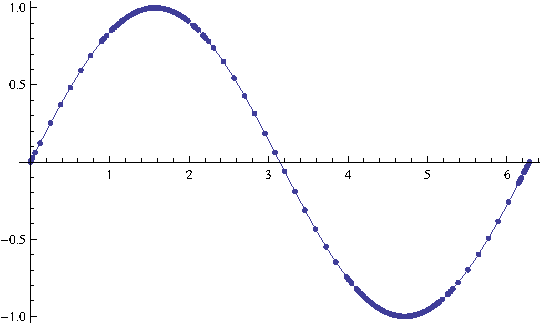
\includegraphics{figures/figmathematica_sinx}
\captionsetup{type=figure}%
			\caption{A graph of $y=\sin x$ generated by \textit{Mathematica}.}\label{fig:mathematica_sinx}
\end{minipage}
\vskip\baselineskip

How does \textit{Mathematica} know where the graph is ``curvy''? Calculus. When we study \textit{curvature} in a later chapter, we will see how the first and second derivatives of a function work together to provide a measurement of ``curviness.'' \textit{Mathematica} employs algorithms to determine regions of ``high curvature'' and plots extra points there.

Again, the goal of this section is not ``How to graph a function when there is no computer to help.'' Rather, the goal is ``Understand that the shape of the graph of a function is largely determined by understanding the behaviour of the function at a few key places.'' In Example \ref{ex_sketch3}, we were able to accurately sketch a complicated graph using only 5 points and knowledge of asymptotes!

There are many applications of our understanding of derivatives beyond curve sketching. The next chapter explores some of these applications, demonstrating just a few kinds of problems that can be solved with a basic knowledge of differentiation. 

\printexercises{exercises/03_05_exercises}
%%
%%%%\addtocounter{chapter}{3}

\clearpage{\pagestyle{empty}\cleardoublepage}
\chapter{Applications of the Derivative}\label{chapter:deriv_apps}
\thispagestyle{empty}

In Chapter \ref{chapter:graphbehavior}, we learned how the first and second derivatives of a function influence its graph. In this chapter we explore other applications of the derivative.


\section{Newton's Method}\label{sec:newton}
Solving equations is one of the most important things we do in mathematics, yet we are surprisingly limited in what we can solve analytically.  For instance, equations as simple as $x^5+x+1=0$ or $\cos x =x $ cannot be solved by algebraic methods in terms of familiar functions.  Fortunately, there are methods that can give us \textit{approximate} solutions to equations like these.  These methods can usually give an approximation correct to as many decimal places as we like. In Section \ref{sec:continuity} we learned about the Bisection Method.  This section focuses on another technique (which generally works faster), called Newton's Method.

%\vspace{.1in}\textbf{Newton's Method}\vspace{.1in}

Newton's Method is built around tangent lines.  The main idea is that if $x$ is sufficiently close to a root of $f(x)$, then the  tangent line to the graph at $(x,f(x))$ will cross the $x$-axis at a point closer to the root than $x$.  


\ifthenelse{\boolean{longpage}}% if longpage, draw in a row
{\noindent\begin{minipage}{.45\textwidth}\centering
\myincludegraphics{figures/fignewt1a} \\ (a)
\end{minipage}\hskip .1\textwidth
\begin{minipage}{.45\textwidth}\centering
\myincludegraphics{figures/fignewt1b} \\ (b)
\end{minipage}

\noindent\begin{minipage}{\textwidth}\centering
\myincludegraphics{figures/fignewt1c} \\ (c)
\captionsetup{type=figure}%
\caption{Demonstrating the geometric concept behind Newton's Method.}\label{fig:newt1}
\end{minipage}
}
{\mtable{.5}{Demonstrating the geometric concept behind Newton's Method. Note how $x_3$ is very close to a solution to $f(x) = 0$.}{fig:newt1}{\begin{tabular}{c}\myincludegraphics{figures/fignewt1a}\\(a)\\\myincludegraphics{figures/fignewt1b} \\ (b) \\ \myincludegraphics{figures/fignewt1c} \\ (c) \end{tabular}
}
}

We start Newton's Method with an initial guess about roughly where the root is.  Call this $x_0$. (See Figure \ref{fig:newt1}(a).)  Draw the tangent line to the graph at $(x_0,f(x_0))$ and see where it meets the $x$-axis. Call this point $x_1$.  Then repeat the process -- draw the tangent line to the graph at $(x_1, f(x_1))$ and see where it meets the $x$-axis. (See Figure \ref{fig:newt1}(b).) Call this point $x_2$.  Repeat the process again to get $x_3$, $x_4$, etc.  This sequence of points will often converge rather quickly to a root of $f$.  

We can use this \textit{geometric} process to create an \textit{algebraic} process.  Let's look at how we found $x_1$.  We started with the tangent line to the graph at $(x_0,f(x_0))$.  The slope of this tangent line is $\fp(x_0)$ and the equation of the line is
\[
y=\fp(x_0)(x-x_0)+f(x_0).
\]
This line crosses the $x$-axis when $y=0$, and the $x$--value where it crosses is what we called $x_1$. So let $y=0$ and replace $x$ with $x_1$, giving the equation: 
\[
 0 = \fp(x_0)(x_1-x_0)+f(x_0).
\] 
Now solve for $x_1$:
\[
x_1=x_0-\frac{f(x_0)}{\fp(x_0)}.
\]
Since we repeat the same geometric process to find $x_2$ from $x_1$, we have
\[
x_2=x_1-\frac{f(x_1)}{\fp(x_1)}.
\]
In general, given an approximation $x_n$, we can find the next approximation, $x_{n+1}$ as follows:
\[
x_{n+1} = x_{n} - \frac{f(x_{n})}{\fp(x_{n})}.
\]

We summarize this process as follows.

\keyidea{idea:Newton}{Newton's Method}
{Let $f$ be a differentiable function on an interval $I$ with a root in $I$. To approximate the value of the root, accurate to $d$ decimal places:\index{Newton's Method}
	\begin{enumerate}
	\item		Choose a value $x_0$ as an initial approximation of the root. (This is often done by looking at a graph of $f$.)
	\item		Create successive approximations iteratively; given an approximation $x_n$, compute the next approximation $x_{n+1}$ as 
	\[
	x_{n+1} = x_n - \frac{f(x_n)}{\fp(x_n)}.
	\]
	\item		Stop the iterations when successive approximations do not differ in the first $d$ places after the decimal point.
		\end{enumerate}
}

\mnote{.75}{\textbf{Note:} Newton's Method is not infallible. The sequence of approximate values may not converge, or it may converge so slowly that one is ``tricked'' into thinking a certain approximation is better than it actually is. These issues will be discussed at the end of the section.}

Let's practice Newton's Method with a concrete example.\\

\example{ex_newt2}{Using Newton's Method}{
Approximate the real root of $x^3-x^2-1=0$,  accurate to the first 3 places after the decimal, using Newton's Method and an initial approximation of $x_0=1$.}
{To begin, we compute $\fp(x)=3x^2-2x$.  Then we apply the Newton's Method algorithm, outlined in Key Idea \ref{idea:Newton}. 
\begin{align*}
x_1&=1-\frac{f(1)}{\fp(1)}=1-\frac{1^3-1^2-1}{3\cdot 1^2-2\cdot 1}=2,\\
x_2&=2-\frac{f(2)}{\fp(2)}=2-\frac{2^3-2^2-1}{3\cdot 2^2-2\cdot 2}=1.625,\\
x_3&=1.625-\frac{f(1.625)}{\fp(1.625)} = 1.625-\frac{1.625^3-1.625^2-1}{3\cdot 1.625^2-2\cdot 1.625}\approx 1.48579. \\
x_4 &= 1.48579 - \frac{f(1.48579)}{\fp(1.48579)} \approx  1.46596\\
x_5 &= 1.46596 - \frac{f(1.46596)}{\fp(1.46596)} \approx 1.46557
\end{align*}
We performed 5 iterations of Newton's Method to find a root accurate to the first 3 places after the decimal; our final approximation is $1.465.$ The exact value of the root, to six decimal places, is $1.465571$;  It turns out that our $x_5$ is accurate to more than just 3 decimal places.

A graph of $f(x)$ is given in Figure \ref{fig:newt2}. We can see from the graph that our initial approximation of $x_0=1$ was not particularly accurate; a closer guess would have been $x_0=1.5$. Our choice was based on ease of initial calculation, and shows that Newton's Method can be robust enough that we do not have to make a very accurate initial approximation.
\mfigure{.5}{A graph of $f(x) = x^3-x^2-1$ in Example \ref{ex_newt2}.}{fig:newt2}{figures/fignewt2}
}\\   

We can automate this process on a calculator that has an \verb+Ans+ key that returns the result of the previous calculation.  Start by pressing \verb+1+ and then \texttt{Enter}. (We have just entered our initial guess, $x_0=1$.)  Now  compute 
\[
\text{\tt Ans} - \frac{f(\text{\tt Ans})}{\fp(\text{\tt Ans})}
\]
 by entering the following and repeatedly press the \texttt{Enter} key:
\begin{center}
\verb+Ans-(Ans^3-Ans^2-1)/(3*Ans^2-2*Ans)+
\end{center}
Each time we press the \texttt{Enter} key, we are finding the successive approximations, $x_1$, $x_2$, \dots, and each one is getting closer to the root.  In fact, once we get past around $x_7$ or so, the approximations don't appear to be changing.  They actually are changing, but the change is far enough to the right of the decimal point that it doesn't show up on the calculator's display.  When this happens, we can be pretty confident that we have found an accurate approximation.

Using a calculator in this manner makes the calculations simple; many iterations can be computed very quickly. \\

%In general, one would usually run Newton's Method in this way, finding approximations until the difference between two successive approximations is less than some prescribed tolerance, like maybe $10^{-10}$, whatever is necessary for the problem at hand.

\example{ex_newt3}{Using Newton's Method to find where functions intersect}{
Use Newton's Method to approximate a solution to $\cos{x} = x$, accurate to 5 places after the decimal.}
{Newton's Method provides a method of solving $f(x) = 0$; it is not (directly) a method for solving equations like $f(x) = g(x)$. However, this is not a problem; we can rewrite the latter equation as $f(x) - g(x)=0$ and then use Newton's Method. 

So we rewrite $\cos x=x$ as $\cos{x}-x=0$.  Written this way, we are finding a root of $f(x)=\cos{x}-x$.  We compute $\fp(x)=-\sin{x} - 1$.  Next we need a starting value, $x_0$.  Consider Figure \ref{fig:newt3}, where $f(x) = \cos x-x$ is graphed. It seems that $x_0=0.75$ is pretty close to the root, so we will use that as our $x_0$. (The figure also shows the graphs of $y=\cos x$ and $y=x$, drawn with dashed lines. Note how they intersect at the same $x$ value as when $f(x) = 0$.)

\mfigure{.65}{A graph of $f(x)=\cos x-x$ used to find an initial approximation of its root.}{fig:newt3}{figures/fignewt3}

We now compute $x_1$, $x_2$, etc.  The formula for $x_1$ is 
\[
x_1 = 0.75 - \frac{\cos(0.75)-0.75}{-\sin(0.75)-1}\approx 0.7391111388.
\]
%To 11 decimal places, this gives .7391111388.  We then compute 
Apply Newton's Method again to find $x_2$:
\[
x_2 = 0.7391111388 - \frac{\cos(0.7391111388)-0.7391111388}{-\sin(0.7391111388)-1}\approx 0.7390851334.
\]
We can continue this way, but it is really best to automate this process.  On a calculator with an Ans key, we would start by pressing 0.75, then \texttt{Enter}, inputting our initial approximation. We then enter:
%\begin{verbatim}
\begin{center}\texttt{Ans - (cos(Ans)-Ans)/(-sin(Ans)-1)}.\end{center}
%\end{verbatim}

Repeatedly pressing the \texttt{Enter} key gives successive approximations.  We quickly find:
\begin{align*}
x_3 &= 0.7390851332\\
x_4 &= 0.7390851332.
\end{align*}
Our approximations $x_2$ and $x_3$ did not differ for at least the first 5 places after the decimal, so we could have stopped. However, using our calculator in the manner described is easy, so finding $x_4$ was not hard. It is interesting to see how we found an approximation, accurate to as many decimal places as our calculator displays, in just 4 iterations.
}\\

If you know how to program, you can translate the following pseudocode into your favourite language to perform the computation in this problem.
\begin{center}
\begin{verbatim}
x = .75
while true
    oldx = x
    x = x - (cos(x)-x)/(-sin(x)-1)
    print x
    if abs(x-oldx) < .0000000001
        break
\end{verbatim}
\end{center}

This code calculates $x_1$, $x_2$, etc., storing each result in the variable \texttt{x}.  The previous approximation is stored in the variable \texttt{oldx}.  We continue looping until the difference between two successive approximations, \texttt{abs(x-oldx)}, is less than some small tolerance, in this case,
\texttt{.0000000001}.\\

\noindent\textbf{\large Convergence of Newton's Method}
\vskip \baselineskip

What should one use for the initial guess, $x_0$?  Generally, the closer to the actual root the initial guess is, the better.  However, some initial guesses should be avoided.  For instance, consider Example \ref{ex_newt2} where we sought the root to $f(x) = x^3-x^2-1$.  Choosing  $x_0=0$ would have been a particularly poor choice. Consider Figure \ref{fig:newt2a}, where $f(x)$ is graphed along with its tangent line at $x=0$. Since $\fp(0)=0$, the tangent line is horizontal and does not intersect the $x$--axis. Graphically, we see that Newton's Method fails.

\mfigure{.8}{A graph of $f(x) = x^3-x^2-1$, showing why an initial approximation of $x_0=0$ with Newton's Method fails.}{fig:newt2a}{figures/fignewt2a}

We can also see analytically that it fails. Since 
\[
x_1 = 0 -\frac{f(0)}{\fp(0)}
\]
 and $\fp(0)=0$, we see that $x_1$ is not well defined.  

This problem can also occur if, for instance, it turns out that $\fp(x_5)=0$. Adjusting the initial approximation $x_0$ by a very small amount will likely fix the problem.

It is also possible for Newton's Method to not converge while each successive approximation is well defined. Consider $f(x) = x^{1/3}$, as shown in Figure \ref{fig:newt4}. It is clear that the root is $x=0$, but let's approximate this with $x_0=0.1$. Figure \ref{fig:newt4}(a) shows graphically the calculation of $x_1$; notice how it is farther from the root than $x_0$. Figures \ref{fig:newt4}(b) and (c) show the calculation of $x_2$ and $x_3$, which are even farther away; our successive approximations are getting worse. (It turns out that in this particular example, each successive approximation is twice as far from the true answer as the previous approximation.)

\ifthenelse{\boolean{longpage}}% if longpage, draw in a row
{\noindent\begin{minipage}{.45\textwidth}\centering
\myincludegraphics{figures/fignewt4a} \\ (a)
\end{minipage}\hskip .1\textwidth
\begin{minipage}{.45\textwidth}\centering
\myincludegraphics{figures/fignewt4b} \\ (b)
\end{minipage}

\noindent\begin{minipage}{\textwidth}\centering
\myincludegraphics{figures/fignewt4c} \\ (c)
\captionsetup{type=figure}%
\caption{Newton's Method fails to find a root of $f(x) = x^{1/3}$, regardless of the choice of $x_0$.}\label{fig:newt4}
\end{minipage}
}% not long page
{\mtable{.4}{Newton's Method fails to find a root of $f(x) = x^{1/3}$, regardless of the choice of $x_0$.}{fig:newt4}{\begin{tabular}{c}\myincludegraphics{figures/fignewt4a}\\(a)\\\myincludegraphics{figures/fignewt4b} \\ (b) \\ \myincludegraphics{figures/fignewt4c} \\ (c) \end{tabular}
}
}

There is no ``fix'' to this problem; Newton's Method simply will not work and another method must be used.


%There are other things that can go wrong with Newton's Method.  For instance, $f(x)=\sqrt[3]{x}$ has a vertical tangent line near its root at $x=0$.  This has the effect of actually pushing the approximations away from the root.  

While Newton's Method does not always work, it does work ``most of the time,'' and it is generally very fast. Once the approximations get close to the root, Newton's Method can as much as double the number of correct decimal places with each successive approximation. A course in Numerical Analysis will introduce the reader to more iterative root finding methods, as well as give greater detail about the strengths and weaknesses of Newton's Method.

%Despite the fact that Newton's Method won't always work, it does work quite often. And it is quick.  A lot of the time, once the approximations get close to the root, Newton's Method can as much as double the number of correct decimal places with each successive approximation.  Newton's Method and other methods that are related to it are what calculators and computer algebras systems use to find approximate solutions to equations.

\printexercises{exercises/04_01_exercises}

\section{Related Rates}\label{sec:related_rates}

When two quantities are related by an equation, knowing the value of one quantity can determine the value of the other. For instance, the circumference and radius of a circle are related by $C=2\pi r$; knowing that $C = 6\pi$in determines the radius must be 3in.

The topic of \sword{related rates} takes this one step further: knowing the \textit{rate} at which one quantity is changing can determine the \textit{rate} at which the other changes.\index{related rates}\\

\mnote{.5}{\textbf{Note:} This section relies heavily on implicit differentiation, so referring back to Section \ref{sec:imp_deriv} may help.}

We demonstrate the concepts of related rates through examples.\\

\example{ex_rr1}{Understanding related rates}{
The radius of a circle is growing at a rate of 5in/hr. At what rate is the circumference growing?}
{The circumference and radius of a circle are related by $C = 2\pi r$. We are given information about how the length of $r$ changes with respect to time; that is, we are told $\frac{dr}{dt} = 5$in/hr. We want to know how the length of $C$ changes with respect to time, i.e., we want to know $\frac{dC}{dt}$. 

Implicitly differentiate both sides of $C = 2\pi r$ with respect to $t$:
\begin{align*}
C 	&= 2\pi r\\
\frac{d}{dt}\big(C\big) &= \frac{d}{dt}\big(2\pi r\big) \\
\frac{dC}{dt} 	&=	2\pi \frac{dr}{dt}.
\end{align*}
As we know $\frac{dr}{dt} = 5$in/hr, we know $$\frac{dC}{dt} = 2\pi 5 = 10\pi \approx 31.4\text{in/hr.}$$
\vskip-\baselineskip}\\

Consider another, similar example.\\

\example{ex_rr2}{Finding related rates}{
Water streams out of a faucet at a rate of $2$in$^3$/s onto a flat surface at a constant rate, forming a circular puddle that is $1/8$in deep. 
\begin{enumerate}
\item		At what rate is the area of the puddle growing?
\item		At what rate is the radius of the circle growing?
\end{enumerate}
}
{\begin{enumerate}
\item We can answer this question two ways: using ``common sense'' or related rates. The common sense method states that the volume of the puddle is growing by $2$in$^3$/s, where 
	\begin{center} volume of puddle $=$ area of circle $\times$ depth.\end{center}
Since the depth is constant at $1/8$in, the area must be growing by 16in$^2$/s.

This approach reveals the underlying related--rates principle. Let $V$ and $A$ represent the Volume and Area of the puddle. We know $V= A\times \frac18$. Take the derivative of both sides with respect to $t$, employing implicit differentiation.
\begin{align*}
V &= \frac18A\\
\frac{d}{dt}\big(V\big) &= \frac{d}{dt}\left(\frac18A\right)\\
\frac{dV}{dt} &=	\frac18\frac{dA}{dt}
\end{align*} 
As $\frac{dV}{dt} = 2$, we know $2 = \frac18\frac{dA}{dt}$, and hence $\frac{dA}{dt} = 16$. Thus the area is growing by 16in$^2$/s.

\drawexampleline
\item		To start, we need an equation that relates what we know to the radius. We just learned something about the surface area of the circular puddle, and we know $A = \pi r^2$. We should be able to learn about the rate at which the radius is growing with this information. 

Implicitly derive both sides of $A=\pi r^2$ with respect to $t$:
\begin{align*}
	A 	&= \pi r^2 \\
	\frac{d}{dt}\big(A\big) &= \frac{d}{dt}\big(\pi r^2\big)\\
	\frac{dA}{dt} &= 2\pi r\frac{dr}{dt}
\end{align*}

Our work above told us that $\frac{dA}{dt} = 16$in$^2$/s. Solving for $\frac{dr}{dt}$, we have $$\frac{dr}{dt} = \frac{8}{\pi r}.$$

Note how our answer is not a number, but rather a function of $r$. In other words, \textit{the rate at which the radius is growing depends on how big the circle already is.} If the circle is very large, adding 2in$^3$ of water will not make the circle much bigger at all. If the circle dime--sized, adding the same amount of water will make a radical change in the radius of the circle.

In some ways, our problem was (intentionally) ill--posed. We need to specify a current radius in order to know a rate of change. When the puddle has a radius of 10in, the radius is growing at a rate of $$
\frac{dr}{dt} = \frac{8}{10\pi} = \frac{4}{5\pi} \approx 0.25\text{in/s}.$$
 
\end{enumerate}
\vskip-2\baselineskip
}\\

\example{ex_rr3}{Studying related rates}{
Radar guns measure the rate of distance change between the gun and the object it is measuring. For instance, a reading of ``55mph'' means the object is moving away from the gun at a rate of 55 miles per hour, whereas a measurement of ``$-25$mph'' would mean that the object is approaching the gun at a rate of 25 miles per hour.

If the radar gun is moving (say, attached to a police car) then radar readouts are only immediately understandable if the gun and the object are moving along the same line. If a police officer is traveling 60mph and gets a readout of 15mph, he knows that the car ahead of him is moving away at a rate of 15 miles an hour, meaning the car is traveling 75mph. (This straight--line principle is one reason officers park on the side of the highway and try to shoot straight back down the road. It gives the most accurate reading.)

Suppose an officer is driving due north at 30 mph and sees a car moving due east, as shown in Figure \ref{fig:rr3}. Using his radar gun, he measures a reading of 20mph. By using landmarks, he believes both he and the other car are about 1/2 mile from the intersection of their two roads. 

\mfigure{.75}{A sketch of a police car (at bottom) attempting to measure the speed of a car (at right) in Example \ref{ex_rr3}.}{fig:rr3}{figures/figrr3}

If the speed limit on the other road is 55mph, is the other driver speeding?}
{Using the diagram in Figure \ref{fig:rr3}, let's label what we know about the situation. As both the police officer and other driver are 1/2 mile from the intersection, we have $A = 1/2$, $B = 1/2$, and through the Pythagorean Theorem, $C = 1/\sqrt{2}\approx 0.707$. 

We know the police officer is traveling at 30mph; that is, $\frac{dA}{dt} = -30$. The reason this rate of change is negative is that $A$ is getting smaller; the distance between the officer and the intersection is shrinking. The radar measurement is $\frac{dC}{dt} = 20$. We want to find $\frac{dB}{dt}$. 

We need an equation that relates $B$ to $A$ and/or $C$. The Pythagorean Theorem is a good choice: $A^2+B^2 = C^2$. Differentiate both sides with respect to $t$:
\begin{align*}
		A^2 + B^2 &= C^2 \\
		\frac{d}{dt}\left(A^2+B^2\right) &= \frac{d}{dt}\left(C^2\right) \\
		2A\frac{dA}{dt} + 2B\frac{dB}{dt} &= 2C\frac{dC}{dt}
\end{align*}

We have values for everything except $\frac{dB}{dt}$. Solving for this we have 
		$$\frac{dB}{dt} = \frac{C\frac{dC}{dt}- A\frac{dA}{dt}}{B} \approx 58.28\text{mph}.$$
		
The other driver appears to be speeding slightly.		
}\\

\mnote{.5}{\textbf{Note:} Example \ref{ex_rr3} is both interesting and impractical. It highlights the difficulty in using radar in a non--linear fashion, and explains why ``in real life'' the police officer would follow the other driver to determine their speed, and not pull out pencil and paper.

The principles here are important, though. Many automated vehicles make judgements about other moving objects based on perceived distances, radar--like measurements and the concepts of related rates.}

\example{ex_rr4}{Studying related rates}{
A camera is placed on a tripod 10ft from the side of a road. The camera is to turn to track a car that is to drive by at 100mph for a promotional video. The video's planners want to know what kind of motor the tripod should be equipped with in order to properly track the car as it passes by.  Figure \ref{fig:rr4} shows the proposed setup.

\mfigure{.25}{Tracking a speeding car (at left) with a rotating camera.}{fig:rr4}{figures/figrr4}

How fast must the camera be able to turn to track the car?
}
{We seek information about how fast the camera is to \textit{turn}; therefore, we need an equation that will relate an angle $\theta$ to the position of the camera and the speed and position of the car.

Figure \ref{fig:rr4} suggests we use a trigonometric equation. Letting $x$ represent the distance the car is from the point on the road directly in front of the camera, we have \begin{equation}\tan \theta = \frac{x}{10}.\label{eq:rr4}\end{equation} As the car is moving at 100mph, we have $\frac{dx}{dt} = -100$mph (as in the last example, since $x$ is getting smaller as the car travels, $\frac{dx}{dt}$ is negative). We need to convert the measurements so they use the same units; rewrite -100mph in terms of ft/s:
$$\frac{dx}{dt} = -100\frac{\text{m}}{\text{hr}} = -100\frac{\text{m}}{\text{hr}}\cdot5280\frac{\text{ft}}{\text{m}}\cdot\frac{1}{3600}\frac{\text{hr}}{\text{s}} =-146.\overline{6}\text{ft/s}.$$
Now take the derivative of both sides of Equation \eqref{eq:rr4} using implicit differentiation:
\begin{align}
		\tan \theta &= \frac{x}{10} \notag \\
		\frac{d}{dt}\big(\tan \theta\big) &= \frac{d}{dt}\left(\frac{x}{10}\right)\notag \\
		\sec^2\theta\,\frac{d\theta}{dt} &= \frac{1}{10}\frac{dx}{dt}\notag\\
		\frac{d\theta}{dt} &= \frac{\cos^2\theta}{10}\frac{dx}{dt}\label{eq:rr4b}
\end{align}
We want to know the fastest the camera has to turn. Common sense tells us this is when the car is directly in front of the camera (i.e., when $\theta = 0$). Our mathematics bears this out. In Equation \eqref{eq:rr4b} we see this is when $\cos^2\theta$ is largest; this is when $\cos \theta = 1$, or when $\theta = 0$.

With $\frac{dx}{dt} \approx -146.67$ft/s, we have 
	$$\frac{d\theta}{dt} = -\frac{1\text{rad}}{10\text{ft}}146.67\text{ft/s} = -14.667\text{radians/s}.$$
We find that $\frac{d\theta}{dt}$ is negative; this matches our diagram in Figure \ref{fig:rr4} for $\theta$ is getting smaller as the car approaches the camera.	
	
What is the practical meaning of $-14.667$radians/s? Recall that 1 circular revolution goes through $2\pi$ radians, thus $14.667$rad/s means $14.667/(2\pi)\approx 2.33$ revolutions per second. The negative sign indicates the camera is rotating in a clockwise fashion.
}\\

We introduced the derivative as a function that gives the slopes of tangent lines of functions. This chapter emphasizes using the derivative in other ways. Newton's Method uses the derivative to approximate roots of functions; this section stresses the ``rate of change'' aspect of the derivative to find a relationship between the rates of change of two related quantities. 

In the next section we use Extreme Value concepts to \textit{optimize} quantities. 

\printexercises{exercises/04_02_exercises}
\section{Optimization}\label{sec:optimization}

In Section \ref{sec:extreme_values} we learned about extreme values -- the largest and smallest values a function attains on an interval. We motivated our interest in such values by discussing how it made sense to want to know the highest/lowest values of a stock, or the fastest/slowest an object was moving. In this section we apply the concepts of extreme values to solve ``word problems,'' i.e., problems stated in terms of situations that require us to create the appropriate mathematical framework in which to solve the problem.\index{optimization}

\enlargethispage{\baselineskip}
We start with a classic example which is followed by a discussion of the topic of optimization.\\

\example{ex_opt1}{Optimization: perimeter and area}{
A man has 100 metres of fencing, a large yard, and a small dog. He wants to create a rectangular enclosure for his dog with the fencing that provides the maximal area. What dimensions provide the maximal area?}
{One can likely guess the correct answer -- that is great. We will proceed to show how calculus can provide this answer in a context that proves this answer is correct.

It helps to make a sketch of the situation. Our enclosure is sketched twice in Figure \ref{fig:opt1}, either with green grass and nice fence boards or as a simple rectangle. Either way, drawing a rectangle forces us to realize that we need to know the dimensions of this rectangle so we can create an area function -- after all, we are trying to maximize the area.

\ifthenelse{\boolean{longpage}}% longpage
{\noindent\begin{center}
\myincludegraphics{figures/figopt1b}
\captionsetup{type=figure}%
\caption{A sketch of the enclosure in Example \ref{ex_opt1}.}\label{fig:opt1}
\end{center}
} % end longpage
{\mfigure{.5}{A sketch of the enclosure in Example \ref{ex_opt1}.}{fig:opt1}{figures/figopt1a}
} %end regular page


We let $x$ and $y$ denote the lengths of the sides of the rectangle. Clearly, 
\[
\text{Area}=xy.
\]

We do not yet know how to handle functions with 2 variables; we need to reduce this down to a single variable. We know more about the situation: the man has 100 metres of fencing. By knowing the perimeter of the rectangle must be 100, we can create another equation: 
\[
\text{Perimeter} = 100 = 2x+2y.
\]

We now have 2 equations and 2 unknowns. In the latter equation, we solve for $y$:
\[
y = 50-x.
\]
 Now substitute this expression for $y$ in the area equation:
\[
 \text{Area} = A(x) = x(50-x).
 \]
  Note we now have an equation of one variable; we can truly call the Area a function of $x$. 

This function only makes sense when $0\leq x \leq 50$, otherwise we get negative values of area. So we find the extreme values of $A(x)$ on the interval $[0,50]$. 

To find the critical points, we take the derivative of $A(x)$ and set it equal to 0, then solve for $x$.
\begin{align*}
A(x) &= x(50-x) \\
			&= 50x-x^2 \\
A'(x) 	&= 50-2x
\end{align*}
We solve $50-2x=0$ to find $x=25$; this is the only critical point. We evaluate $A(x)$ at the endpoints of our interval and at this critical point to find the extreme values; in this case, all we care about is the maximum.

Clearly $A(0)=0$ and $A(50)=0$, whereas $A(25) = 625 \text{m}^2$. This is the maximum. Since we earlier found $y = 50-x$, we find that $y$ is also $25$. Thus the dimensions of the rectangular enclosure with perimeter of 100 m with maximum area is a square, with sides of length 25 m.
}\\

This example is very simplistic and a bit contrived. (After all, most people create a design then buy fencing to meet their needs, and not buy fencing and plan later.) But it models well the necessary process: create equations that describe a situation, reduce an equation to a single variable, then find the needed extreme value.

``In real life,'' problems are much more complex. The equations are often \textit{not} reducible to a single variable (hence multi--variable calculus is needed) and the equations themselves may be difficult to form. Understanding the principles here will provide a good foundation for the mathematics you will likely encounter later.

We outline here the basic process of solving these optimization problems.
\enlargethispage{2\baselineskip}
%\small
\keyidea{idea:optimization}{Solving Optimization Problems}
{\begin{enumerate}
		\item		Understand the problem. Clearly identify what quantity is to be maximized or minimized. Make a sketch if helpful.
		\item		Create equations relevant to the context of the problem, using the information given. (One of these should describe the quantity to be optimized. We'll call this the \textit{fundamental equation.})
		\item		If the fundamental equation defines the quantity to be optimized as a function of more than one variable, reduce it to a single variable function using substitutions derived from the other equations.
		\item		Identify the domain of this function, keeping in mind the context of the problem.
		\item		Find the extreme values of this function on the determined domain.
		\item		Identify the values of all relevant quantities of the problem.
		\end{enumerate}
}
%\normalsize

We will use Key Idea \ref{idea:optimization} in a variety of examples.\\

\example{ex_opt2}{Optimization: perimeter and area}{
Here is another classic calculus problem: A woman has a 100 metres of fencing, a small dog, and a large yard that contains a stream (that is mostly straight). She wants to create a rectangular enclosure with maximal area that uses the stream as one side. (Apparently her dog won't swim away.) What dimensions provide the maximal area?}
{We will follow the steps outlined by Key Idea \ref{idea:optimization}. 
	\begin{enumerate}
	\item		We are maximizing \textit{area}. A sketch of the region will help; Figure \ref{fig:opt2} gives two sketches of the proposed enclosed area. A key feature of the sketches is to acknowledge that one side is not fenced. 
	
\mfigure{.4}{A sketch of the enclosure in Example \ref{ex_opt2}.}{fig:opt2}{figures/figopt2a}
	
	\item		We want to maximize the area; as in the example before, 
	\[
	\text{Area} = xy.
	\]
 This is our fundamental equation. This defines area as a function of two variables, so we need another equation to  reduce it to one variable. 
	
	We again appeal to the perimeter; here the perimeter is 
	\[
	\text{Perimeter} = 100 = x+2y.
	\]
 Note how this is different than in our previous example.
	\item		We now reduce the fundamental equation to a single variable. In the perimeter equation, solve for $y$: $y = 50 - x/2$. We can now write Area as 
	\[
	\text{Area} = A(x) = x(50-x/2) = 50x - \frac12x^2.
	\]
 Area is now defined as a function of one variable.
	\item		We want the area to be nonnegative. Since $A(x) = x(50-x/2)$, we want $x\geq 0$ and $50-x/2\geq 0$. The latter inequality implies that $x\leq100$, so $0\leq x\leq 100$. 
	\item		We now find the extreme values. At the endpoints, the minimum is found, giving an area of 0. 
	
	Find the critical points. We have $A'(x) = 50-x$; setting this equal to 0 and solving for $x$ returns $x=50$. This gives an area of 
	\[
	A(50) = 50(25) = 1250.
	\]
	\item		We earlier set $y = 50-x/2$; thus $y = 25$. Thus our rectangle will have two sides of length 25 and one side of length 50, with a total area of 1250 m$^2$.
	\end{enumerate}
\vskip-\baselineskip
}\\

Keep in mind as we do these problems that we are practising a \textit{process}; that is, we are learning to turn a situation into a system of equations. These equations allow us to write a certain quantity as a function of one variable, which we then optimize.\\

%\mnote{.5}{\textbf{Note:} Example \ref{ex_opt3} is another classic calculus example. The underlying principle is given in a variety of contexts; Google ``calculus dog'' to find articles where 

\example{ex_opt3}{Optimization: minimizing cost}{
A power line needs to be run from an power station located on the beach to an offshore facility. Figure \ref{fig:opt3b} shows the distances between the power station to the facility.

It costs \$50/ft. to run a power line along the land, and \$130/ft. to run a power line under water. How much of the power line should be run along the land to minimize the overall cost? What is the minimal cost?

\mfigure{.3}{Running a power line from the power station to an offshore facility with minimal cost in Example \ref{ex_opt3}.}{fig:opt3b}{figures/figopt3b}
}
{We will follow the strategy of Key Idea \ref{idea:optimization} implicitly, without specifically numbering steps.

There are two immediate solutions that we could consider, each of which we will reject through ``common sense.'' First, we could minimize the distance by directly connecting the two locations with a straight line. However, this requires that all the wire be laid underwater, the most costly option. Second, we could minimize the underwater length by running a wire all 5000 ft. along the beach, directly across from the offshore facility. This has the undesired effect of having the longest distance of all, probably ensuring a non--minimal cost.

The optimal solution likely has the line being run along the ground for a while, then underwater, as the figure implies. We need to label our unknown distances -- the distance run along the ground and the distance run underwater. Recognizing that the underwater distance can be measured as the hypotenuse of a right triangle, we choose to label the distances as shown in Figure \ref{fig:opt3c}.

\mfigure{.15}{Labelling unknown distances in Example \ref{ex_opt3}.}{fig:opt3c}{figures/figopt3c}

By choosing $x$ as we did, we make the expression under the square root simple. We now create the cost function. 

\[
\begin{array}{ccccc}
\text{Cost} &=&  \text{land cost} &+ & \text{water cost} \\
						&	& \text{\$50}\times \text{land distance} &+& \text{\$130}\times \text{water distance} \\
						&	& 50(5000-x) &+& 130\sqrt{x^2+1000^2}.\\
\end{array}
\]

So we have $c(x) = 50(5000-x)+ 130\sqrt{x^2+1000^2}$. This function only makes sense on the interval $[0,5000]$. While we are fairly certain the endpoints will not give a minimal cost, we still evaluate $c(x)$ at each to verify.
\[
c(0) = 380,000 \quad\quad c(5000) \approx 662,873.
\]

We now find the critical values of $c(x)$. We compute $c\primeskip'(x)$ as 
\[
c\primeskip'(x) = -50+\frac{130x}{\sqrt{x^2+1000^2}}.
\]

Recognize that this is never undefined. Setting $c\primeskip'(x)=0$ and solving for $x$, we have:
\begin{align*}
-50+\frac{130x}{\sqrt{x^2+1000^2}} &= 0 \\
\frac{130x}{\sqrt{x^2+1000^2}}  &= 50\\
\frac{130^2x^2}{x^2+1000^2} &= 50^2\\
130^2x^2 &= 50^2(x^2+1000^2) \\
130^2x^2-50^2x^2 &= 50^2\cdot1000^2\\
(130^2-50^2)x^2 &= 50,000^2\\
x^2 &= \frac{50,000^2}{130^2-50^2}\\
x &= \frac{50,000}{\sqrt{130^2-50^2}}\\
x & = \frac{50,000}{120} =416\frac23\approx 416.67.
\end{align*}

Evaluating $c(x)$ at $x=416.67$ gives a cost of about \$370,000. The distance the power line is laid along land is $5000-416.67 = 4583.33$ ft., and the underwater distance is $\sqrt{416.67^2+1000^2} \approx 1083$ ft.
%\mnote{.5}{\textbf{Note:} This minimal cost is \$10,000 less than the cost of simply minimizing the underwater distance, a savings of about 3\%. Is t
}\\

In the exercises you will see a variety of situations that require you to combine problem--solving skills with calculus. Focus on the \textit{process}; learn how to form equations from situations that can be manipulated into what you need. Eschew memorizing how to do ``this kind of problem'' as opposed to ``that kind of problem.'' Learning a process will benefit one far longer than memorizing a specific technique.

The next section introduces our final application of the derivative: \textit{differentials}. Given $y=f(x)$, they offer a method of approximating the change in $y$ after $x$ changes by a small amount. 

\printexercises{exercises/04_03_exercises}
		
\section{Differentials}\label{sec:differentials}

In Section \ref{sec:interp_deriv} we explored the meaning and use of the derivative. This section starts by revisiting some of those ideas.

Recall that the derivative of a function $f$ can be used to find the slopes of lines tangent to the graph of $f$. At $x=c$, the tangent line to the graph of $f$ has equation 
\[
y = \fp(c)(x-c)+f(c).
\]
The tangent line can be used to find good approximations of $f(x)$ for values of $x$ near $c$. 

For instance, we can approximate $\sin 1.1$ using the tangent line to the graph of $f(x)=\sin x$ at $x=\pi/3 \approx 1.05.$ Recall that $\sin (\pi/3) = \sqrt{3}/2 \approx 0.866$, and $\cos (\pi/3) = 1/2$. Thus the tangent line to $f(x) = \sin x$ at $x=\pi/3$ is: 
\[
 \ell(x) = \frac12(x-\pi/3)+0.866.
\]



\ifthenelse{\boolean{longpage}}% if longpage, draw in a row
{\noindent%
\begin{minipage}{\textwidth}\centering
\noindent\begin{minipage}{.45\textwidth}\centering
\noindent\myincludegraphics{figures/figdiffal1a} \\ (a)
\end{minipage}\hskip .05\textwidth
\begin{minipage}{.45\textwidth}\centering
\noindent\myincludegraphics{figures/figdiffal1} \\ (b)
\end{minipage}
\captionsetup{type=figure}%
\caption{Graphing $f(x) = \sin x$ and its tangent line at $x=\pi/3$ in order to estimate $\sin 1.1$.}\label{fig:diffal1}
\end{minipage}
}
{\mtable{.5}{Graphing $f(x) = \sin x$ and its tangent line at $x=\pi/3$ in order to estimate $\sin 1.1$.}{fig:diffal1}{\begin{tabular}{c}
\myincludegraphics{figures/figdiffal1a}\\[10pt]
(a)\\[10pt]
\myincludegraphics{figures/figdiffal1} \\[10pt]
 (b)\end{tabular}
}
}

In Figure \ref{fig:diffal1}(a), we see a graph of $f(x) = \sin x$ graphed along with its tangent line at $x=\pi/3$. The small rectangle shows the region that is displayed in Figure \ref{fig:diffal1}(b). In this figure, we see how we are approximating $\sin 1.1$ with the tangent line, evaluated at $1.1$. Together, the two figures show how close these values are.

Using this line to approximate $\sin 1.1$, we have:
\begin{align*}
	\ell(1.1) &= \frac12(1.1-\pi/3)+0.866 \\
					&= \frac12(0.053)+0.866 = 0.8925.
\end{align*}
(We leave it to the reader to see how good of an approximation this is.)\\

We now generalize this concept. Given $f(x)$ and an $x$--value $c$,  the tangent line is $\ell(x) = \fp(c)(x-c)+f(c)$. Clearly, $f(c) = \ell(c)$. Let $\dx$ be a small number, representing a small change in $x$ value. We assert that:
\[
f(c+\dx) \approx \ell(c+\dx),
\]
 since the tangent line to a function approximates well the values of that function near $x=c$. 

As the $x$ value changes from $c$ to $c+\dx$, the $y$ value of $f$ changes from $f(c)$ to $f(c+\dx)$. We call this change of $y$ value \dy. That is:
\[
\dy = f(c+\dx)-f(c).
\]
Replacing $f(c+\dx)$ with its tangent line approximation, we have 
\begin{align} \dy &\approx \ell(c+\dx) - f(c) \notag\\
								&= \fp(c)\big((c+\dx)-c\big)+f(c) - f(c)\notag \\
								&=\fp(c)\dx		\label{eq:differential}
\end{align}

This final equation is important; it becomes the basis of the upcoming Definition and Key Idea. In short, it says that when the $x$-value changes from $c$ to $c+\Delta x$, the $y$ value of a function $f$ changes by about $\fp(c)\Delta x$.

We introduce two new variables, $dx$ and $dy$ in the context of a formal definition. %We defined $dx = \dx$; that is, it is a small change in $x$. We define

\definition{def:differential}{Differentials of $x$ and $y$.}
{Let $y=f(x)$ be differentiable. The \textbf{differential of $x$}, denoted $dx$, is any nonzero real number (usually taken to be a small number).\index{differential}\index{derivative!differential} The \textbf{differential of $y$}, denoted $dy$, is 
\[
dy = \fp(x)dx.
\]
}

We can solve for $\fp(x)$ in the above equation: $\fp(x) = dy/dx$. This states that the derivative of $f$ with respect to $x$ is the differential of $y$ divided by the differential of $x$; this is \textbf{not} the alternate notation for the derivative, $\frac{dy}{dx}$. This latter notation was chosen because of the fraction--like qualities of the derivative, but again, it is one symbol and not a fraction.

It is helpful to organize our new concepts and notations in one place.

\keyidea{idea:differential}{Differential Notation}
{Let $y = f(x)$ be a differentiable function. \index{differential!notation}
\begin{enumerate}
	\item Let $\dx$ represent a small, nonzero change in $x$ value.
	\item	Let $dx$ represent a small, nonzero change in $x$ value (i.e., $\dx = dx$).
	\item	Let $\dy$ be the change in $y$ value as $x$ changes by $\dx$; hence 
\[
\dy = f(x+\dx)-f(x).
\]
	\item		Let $dy = \fp(x)dx$ which, by Equation (\ref{eq:differential}), is an \textit{approximation} of the change in $y$ value as $x$ changes by $\dx$; $dy \approx \dy$.
\end{enumerate}
}

What is the value of differentials? Like many mathematical concepts, differentials provide both practical and theoretical benefits. We explore both here.\\

\example{ex_diffal1}{Finding and using differentials}{
Consider $f(x) = x^2$. Knowing $f(3) = 9$, approximate $f(3.1)$.}
{The $x$ value is changing from $x=3$ to $x=3.1$; therefore, we see that $dx=0.1$. If we know how much the $y$ value changes from $f(3)$ to $f(3.1)$ (i.e., if we know $\dy$), we will know exactly what $f(3.1)$ is (since we already know $f(3)$). We can approximate \dy\ with $dy$.
\begin{align*} \dy &\approx dy \\
								  &= \fp(3)dx \\
								  &= 2\cdot 3\cdot 0.1 = 0.6.
\end{align*}

We expect the $y$ value to change by about $0.6$, so we approximate $f(3.1) \approx 9.6.$

We leave it to the reader to verify this, but the preceding discussion links the differential to the tangent line of $f(x)$ at $x=3$. One can verify that the tangent line, evaluated at $x=3.1$, also gives $y=9.6$.
}\\

Of course, it is easy to compute the actual answer (by hand or with a calculator): $3.1^2 = 9.61.$ (Before we get too cynical and say ``Then why bother?'', note our approximation is \textit{really} good!)

So why bother?

In ``most'' real life situations, we do not know the function that describes a particular behaviour. Instead, we can only take measurements of how things change -- measurements of the derivative.

Imagine water flowing down a winding channel. It is easy to measure the speed and direction (i.e., the \textit{velocity}) of water at any location. It is very hard to create a function that describes the overall flow, hence it is hard to predict where a floating object placed at the beginning of the channel will end up. However, we can \textit{approximate} the path of an object using differentials. Over small intervals, the path taken by a floating object is essentially linear. Differentials allow us to approximate the true path by piecing together lots of short, linear paths. This technique is called Euler's Method, studied in introductory Differential Equations courses.

We use differentials once more to approximate the value of a function. Even though calculators are very accessible, it is neat to see how these techniques can sometimes be used to easily compute something that looks rather hard.\\

%\enlargethispage{\baselineskip}

\example{ex_diffal2}{Using differentials to approximate a function value}{
Approximate $\sqrt{4.5}$.}
{We expect $\sqrt{4.5} \approx 2$, yet we can do better. Let $f(x) = \sqrt{x}$, and let $c=4$. Thus $f(4) = 2$. We can compute $\fp(x) = 1/(2\sqrt{x})$, so $\fp(4) = 1/4$. 

We approximate the difference between $f(4.5)$ and $f(4)$ using differentials, with $dx = 0.5$:
\[
f(4.5)-f(4) = \dy \approx dy = \fp(4)\cdot dx = 1/4 \cdot 1/2 = 1/8 = 0.125.
\]
The approximate change in $f$ from $x=4$ to $x=4.5$ is $0.125$, so we approximate $\sqrt{4.5} \approx 2.125.$
}\\

Differentials are important when we discuss \textit{integration}. When we study that topic, we will use notation such as 
\[
\int f(x)\ dx
\]
 quite often. While we don't discuss here what all of that notation means, note the existence of the differential $dx$. Proper handling of \textit{integrals} comes with proper handling of differentials. 

In light of that, we practise finding differentials in general.\\

\example{ex_diffal3}{Finding differentials}{
In each of the following, find the differential $dy$.

\begin{center}
1. $y = \sin x$ \qquad\quad 2. $y = e^x(x^2+2)$ \quad\qquad 3. $y = \sqrt{x^2+3x-1}$
\end{center}
}
{\begin{enumerate}
\item		$y = \sin x$:	\quad As $f(x) = \sin x$, $\fp(x) = \cos x$. Thus 
\[
dy = \cos (x)dx.
\]

\item		$y = e^x(x^2+2)$:\quad Let $f(x) = e^x(x^2+2)$. We need $\fp(x)$, requiring the Product Rule. 

We have $\fp(x) = e^x(x^2+2) + 2xe^x$, so 
\[
dy = \big(e^x(x^2+2) + 2xe^x\big)dx.
\]

\item		$y = \sqrt{x^2+3x-1}$:\quad	Let $f(x) = \sqrt{x^2+3x-1}$; we need $\fp(x)$, requiring the Chain Rule.

We have $\ds \fp(x) = \frac{1}{2}(x^2+3x-1)^{-\frac12}(2x+3) = \frac{2x+3}{2\sqrt{x^2+3x-1}}.$ Thus 
\[
 dy = \frac{(2x+3)dx}{2\sqrt{x^2+3x-1}}.
\]
\end{enumerate}
\vskip-\baselineskip
}\\
%\clearpage

Finding the differential $dy$ of $y=f(x)$ is really no harder than finding the derivative of $f$; we just \textit{multiply} $\fp(x)$ by $dx$. It is important to remember that we are not simply adding the symbol ``$dx$'' at the end.\\

We have seen a practical use of differentials as they offer a good method of making certain approximations. Another use is \textit{error propagation.} Suppose a length is measured to be $x$, although the actual value is $x+\dx$ (where \dx\ is the error, which we hope  is small). This measurement of $x$ may be used to compute some other value; we can think of this latter value as $f(x)$ for some function $f$. As the true length is $x+\dx$, one really should have computed $f(x+\dx)$. The difference between $f(x)$ and $f(x+\dx)$ is the propagated error. 

How close are $f(x)$ and $f(x+\dx)$? This is a difference in ``y'' values:
\[
f(x+\dx)-f(x) = \dy \approx dy.
\]
 We can approximate the propagated error using differentials.\\

\example{ex_diffal4}{Using differentials to approximate propagated error}{
A steel ball bearing is to be manufactured with a diameter of 2cm. The manufacturing process has a tolerance of $\pm 0.1$mm in the diameter. Given that the density of steel is about 7.85g/cm$^3$, estimate the propagated error in the mass of the ball bearing.}
{The mass of a ball bearing is found using the equation ``mass = volume $\times$ density.'' In this situation the mass function is a product of the radius of the ball bearing, hence it is $m = 7.85\frac43\pi r^3$. The differential of the mass is 
\[
dm = 31.4\pi r^2 dr.
\]
 The radius is to be 1 cm; the manufacturing tolerance in the radius is $\pm 0.05$mm, or $\pm 0.005$cm. The propagated error is approximately:
\begin{align*}
\Delta m & \approx dm \\
				&= 31.4\pi (1)^2 (\pm 0.005) \\
				&= \pm 0.493\text{g}
\end{align*}
Is this error significant? It certainly depends on the application, but we can get an idea by computing the \textit{relative error}. The ratio between amount of error to the total mass is
\begin{align*}
\frac{dm}{m} &= \pm \frac{0.493}{7.85\frac43\pi} \\
							&=\pm \frac{0.493}{32.88}\\
							&=\pm 0.015,
\end{align*}
or $\pm 1.5$\%. 

\enlargethispage{\baselineskip}

We leave it to the reader to confirm this, but if the diameter of the ball was supposed to be 10 cm, the same manufacturing tolerance would give a propagated error in mass of $\pm12.33$g, which corresponds to a \textit{percent error} of $\pm0.188$\%. While the amount of error is much greater ($12.33 > 0.493$), the percent error is much lower.
}\\

In this section, we've seen that differentials give us a useful way of approximating complicated functions. In the next section, we'll see that these approximations can be improved by considering higher-degree polynomials, called Taylor Polynomials.

%\refstepcounter{definitioncounter}
%\label{lastdefcount1}
%\refstepcounter{theoremcounter}
%\label{lastthmcount1}
%\refstepcounter{keyideacounter}
%\label{lastideacount1}
%\addtocounter{definitioncounter}{-1}
%\addtocounter{theoremcounter}{-1}
%\addtocounter{keyideacounter}{-1}
%\refstepcounter{examplecounter}
%\label{lastexamplecount1}
%\addtocounter{examplecounter}{-1}

\printexercises{exercises/04_04_exercises}

\section{Taylor Polynomials}\label{sec:taylor_poly1}

Consider a function $y=f(x)$ and a point $\big(c,f(c)\big)$. The derivative, $\fp(c)$, gives the instantaneous rate of change of $f$ at $x=c$. Of all lines that pass through the point $\big(c,f(c)\big)$, the line that best approximates $f$ at this point is the tangent line; that is, the line whose slope (rate of change) is $\fp(c)$.

In Figure \ref{fig:taypoly1introa1}, we see a function $y=f(x)$ graphed. The table below the graph shows that $f(0)=2$ and $\fp(0) = 1$; therefore, the tangent line to $f$ at $x=0$ is $p_1(x) = 1(x-0)+2 = x+2$. The tangent line is also given in the figure. Note that ``near'' $x=0$, $p_1(x) \approx f(x)$; that is, the tangent line approximates $f$ well.

\mtable{.78}{Plotting $y=f(x)$ and a table of derivatives of $f$ evaluated at 0.}{fig:taypoly1introa1}{%
\begin{tabular}{c}
\myincludegraphics{figures/figtaypolyintroa}\\
\\
\begin{tabular}{lll}
$f(0) = 2$ & &$\fp''(0) = -1$\\
$\fp(0) = 1$ &&	$f\,^{(4)}(0)=-12$ \\
$\fpp(0) = 2$ && $f\,^{(5)}(0)=-19$
\end{tabular}
\end{tabular}
}

One shortcoming of this approximation is that the tangent line only matches the slope of $f$; it does not, for instance, match the concavity of $f$. We can find a polynomial, $p_2(x)$, that does match the concavity without much difficulty, though. The table in Figure \ref{fig:taypoly1introa1} gives the following information:
$$f(0) = 2 \qquad \fp(0) = 1\qquad \fp'(0) = 2.$$
Therefore, we want our polynomial $p_2(x)$ to have these same properties. That is, we need $$p_2(0) = 2 \qquad p_2'(0) = 1 \qquad p_2''(0) = 2.$$

This is simply an initial--value problem. We can solve this using the techniques first described in Section \ref{sec:antider}. To keep $p_2(x)$ as simple as possible, we'll assume that not only  $p_2''(0)=2$, but that $p_2''(x)=2$. That is, the second derivative of $p_2$ is  constant.

If $p_2''(x) = 2$, then $p_2'(x) = 2x+C$ for some constant $C$. Since we have determined that $p_2'(0) = 1$, we find that $C=1$ and so $p_2'(x) = 2x+1$. Finally, we can compute $p_2(x) = x^2+x+C$. Using our initial values, we know $p_2(0) = 2$ so $C=2.$ We conclude that $p_2(x) = x^2+x+2.$ This function is plotted with $f$ in Figure \ref{fig:taypoly1introb1}.

\mfigure{.52}{Plotting $f$, $p_2$ and $p_4$.}{fig:taypoly1introb1}{figures/figtaypolyintrob}
\mfigure{.3}{Plotting $f$ and $p_{13}$.}{fig:taypoly1introc1}{figures/figtaypolyintroc}

We can repeat this approximation process by creating polynomials of higher degree that match more of the derivatives of $f$ at $x=0$. In general, a polynomial of degree $n$ can be created to match the first $n$ derivatives of $f$. Figure \ref{fig:taypoly1introb1} also shows $p_4(x)= -x^4/2-x^3/6+x^2+x+2$, whose first four derivatives at 0 match those of $f$. (Using the table in Figure \ref{fig:taypoly1introa1}, start with $p_4^{(4)}(x)=-12$ and solve the related initial--value problem.)

As we use more and more derivatives, our polynomial approximation to $f$ gets better and better. In this example, the interval on which the approximation is ``good'' gets bigger and bigger. Figure \ref{fig:taypoly1introc1} shows $p_{13}(x)$; we can visually affirm that this polynomial approximates $f$ very well on $[-2,3]$. (The polynomial $p_{13}(x)$ is not particularly ``nice''. It is {\scriptsize $$ \frac{16901x^{13}}{6227020800}+\frac{13x^{12}}{1209600}-\frac{1321x^{11}}{39916800}-\frac{779x^{10}}{1814400}-\frac{359x^9}{362880}+\frac{x^8}{240}+\frac{139x^7}{5040}+\frac{11 x^6}{360}-\frac{19x^5}{120}-\frac{x^4}{2}-\frac{x^3}{6}+x^2+x+2.)$$}

The polynomials we have created are examples of \emph{Taylor polynomials}, named after the British mathematician Brook Taylor who made important discoveries about such functions. While we created the above Taylor polynomials by solving initial--value problems, it can be shown that Taylor polynomials follow a general pattern that make their formation much more direct. This is described in the following definition.

\setboxwidth{50pt}
\noindent%\hskip-50pt
\begin{minipage}{\specialboxlength}
\definition{def:taypoly1}{Taylor Polynomial, Maclaurin Polynomial}
{Let $f$ be a function whose first $n$ derivatives exist at $x=c$.
\index{Taylor Polynomial!definition}\index{Maclaurin Polynomial!definition} \index{Maclaurin Polynomial|see{Taylor Polynomial}}
\begin{enumerate}
\item		The \textbf{Taylor polynomial of degree $n$ of $f$ at $x=c$} is 
				{$$p_n(x) = f(c) + \fp(c)(x-c) + \frac{\fpp(c)}{2!}(x-c)^2+\frac{\fp''(c)}{3!}(x-c)^3+\cdots+\frac{f\,^{(n)}(c)}{n!}(x-c)^n.$$}

\item		A special case of the Taylor polynomial is the Maclaurin polynomial, where $c=0$. That is, the \textbf{Maclaurin polynomial of degree $n$ of $f$} is 
{$$p_n(x) = f(0) + \fp(0)x + \frac{\fpp(0)}{2!}x^2+\frac{\fp''(0)}{3!}x^3+\cdots+\frac{f\,^{(n)}(0)}{n!}x^n.$$}
\end{enumerate}
}
\end{minipage}
\restoreboxwidth

We will practice creating Taylor and Maclaurin polynomials in the following examples.\\

\example{ex_taypoly11}{Finding and using Maclaurin polynomials}{
\begin{enumerate}
\item		Find the $n^\text{th}$ Maclaurin polynomial for $f(x) = e^x$.
\item		Use $p_5(x)$ to approximate the value of $e$.
\end{enumerate}
}
{\begin{enumerate}
\item We start with creating a table of the derivatives of $e^x$ evaluated at $x=0$. In this particular case, this is relatively simple, as shown in Figure \ref{fig:taypoly11a}.
\mtable{.58}{The derivatives of $f(x)=e^x$ evaluated at $x=0$.}{fig:taypoly11a}{%
\begin{tabular}{lll}
$f(x) = e^x $&$\Rightarrow $&$f(0) = 1$\\
$\fp(x) = e^x $&$\Rightarrow $&$\fp(0) = 1$\\
$\fp'(x) = e^x $&$\Rightarrow $&$\fp'(0) = 1$\\
$\ \vdots $& &$\ \vdots$\\
$f\,^{(n)}(x) = e^x $&$\Rightarrow $&$f\,^{(n)}(0) = 1$
\end{tabular}
}
By the definition of the Maclaurin series, we have 

\begin{align*}
p_n(x) &= f(0) + \fp(0)x + \frac{\fpp(0)}{2!}x^2+\frac{\fp''(0)}{3!}x^3+\cdots+\frac{f\,^n(0)}{n!}x^n\\
			&= 1+x+\frac{1}{2}x^2+\frac{1}{6}x^3 + \frac{1}{24}x^4 + \cdots + \frac{1}{n!}x^n.
\end{align*}

\item	Using our answer from part 1, we have $$p_5 = 1+x+\frac{1}{2}x^2+\frac{1}{6}x^3 + \frac{1}{24}x^4 + \frac{1}{120}x^5.$$ To approximate the value of $e$, note that $e = e^1 = f(1) \approx p_5(1).$ It is very straightforward to evaluate $p_5(1)$:
$$p_5(1) = 1+1+\frac12+\frac16+\frac1{24}+\frac1{120} = \frac{163}{60} \approx 2.71667.$$

A plot of $f(x)=e^x$ and $p_5(x)$ is given in Figure \ref{fig:taypoly11b}.
\mfigure{.3}{A plot of $f(x)=e^x$ and its 5$^\text{th}$ degree Maclaurin polynomial $p_5(x)$.}{fig:taypoly11b}{figures/figtaypoly1b}
\end{enumerate}
\vskip-1.5\baselineskip
}\\

\example{ex_taypoly12}{Finding and using Taylor polynomials}{
\begin{enumerate}
\item		Find the $n^\text{th}$ Taylor polynomial of $y=\ln x$ at $x=1$.
\item		Use $p_6(x)$ to approximate the value of $\ln 1.5$.
\item		Use $p_6(x)$ to approximate the value of $\ln 2$. 
\end{enumerate}
}
{\begin{enumerate}
\item		We begin by creating a table of derivatives of $\ln x$ evaluated at $x=1$. While this is not as straightforward as it was in the previous example, a pattern does emerge, as shown in Figure \ref{fig:taypoly12a}.
\mtable{.75}{Derivatives of $\ln x$ evaluated at $x=1$.}{fig:taypoly12a}{%
\begin{tabular}{lll}
$f(x) = \ln x $&$\Rightarrow $&$f(1) = 0$\\
$\fp(x) = 1/x $&$\Rightarrow $&$\fp(1) = 1$\\
$\fp'(x) = -1/x^2 $&$\Rightarrow $&$\fp'(1) = -1$\\
$\fp''(x) = 2/x^3 $&$\Rightarrow $&$\fp''(1) = 2$\\
$f\,^{(4)}(x) = -6/x^4 $&$\Rightarrow $&$f\,^{(4)}(1) = -6$\\
$\ \vdots $& &$\ \vdots$\\
$f\,^{(n)}(x) = $ &$\Rightarrow$ & $f\,^{(n)}(1) = $\\
$\ds \rule{0pt}{15pt}\frac{(-1)^{n+1}(n-1)!}{x^n} $ & & $(-1)^{n+1}(n-1)!$
\end{tabular}
%\begin{tabular}{l}
%{\scriptsize $f\,^{(n)}(x) = \frac{(-1)^{n+1}(n-1)!}{x^n} \Rightarrow f\,^{(n)}(1) = (-1)^{n+1}(n-1)!$}
%\end{tabular}
}

Using Definition \ref{def:taypoly1}, we have \small
\begin{align*}
	p_n(x) &=	f(c) + \fp(c)(x-c) + \frac{\fpp(c)}{2!}(x-c)^2+\frac{\fp''(c)}{3!}(x-c)^3+\cdots+\frac{f\,^n(c)}{n!}(x-c)^n\\
					&= 0+(x-1)-\frac12(x-1)^2+\frac13(x-1)^3-\frac14(x-1)^4+\cdots+\frac{(-1)^{n+1}}{n}(x-1)^n.
\end{align*}
\normalsize
Note how the coefficients of the $(x-1)$ terms turn out to be ``nice.''

\item		We can compute $p_6(x)$ using our work above:
$$p_6(x) = (x-1)-\frac12(x-1)^2+\frac13(x-1)^3-\frac14(x-1)^4+\frac15(x-1)^5-\frac16(x-1)^6.$$
Since $p_6(x)$ approximates $\ln x$ well near $x=1$, we approximate $\ln 1.5 \approx p_6(1.5)$:

\begin{align*}
p_6(1.5) &= (1.5-1)-\frac12(1.5-1)^2+\frac13(1.5-1)^3-\frac14(1.5-1)^4+\cdots \\
			&\cdots +\frac15(1.5-1)^5-\frac16(1.5-1)^6\\
	&=\frac{259}{640}\\
	&\approx 0.404688.
\end{align*}
\normalsize
This is a good approximation as a calculator shows that $\ln 1.5 \approx 0.4055.$ Figure \ref{fig:taypoly12b} plots $y=\ln x$ with $y=p_6(x)$. We can see that $\ln 1.5\approx p_6(1.5)$.

\mfigure{.5}{A plot of $y=\ln x$ and its 6$^\text{th}$ degree Taylor polynomial at $x=1$.}{fig:taypoly12b}{figures/figtaypoly2b}
\item	
We approximate $\ln 2$ with $ p_6(2)$:
\begin{align*}
p_6(2) &= (2-1)-\frac12(2-1)^2+\frac13(2-1)^3-\frac14(2-1)^4+\cdots \\
			&\cdots +\frac15(2-1)^5-\frac16(2-1)^6\\
			&=	1-\frac12+\frac13-\frac14+\frac15-\frac16 \\
			&= \frac{37}{60}\\ 
			&\approx 0.616667.
\end{align*}
This approximation is not terribly impressive: a hand held calculator shows that $\ln 2 \approx 0.693147.$ The graph in Figure \ref{fig:taypoly12b} shows that $p_6(x)$ provides less accurate approximations of $\ln x$ as $x$ gets close to 0 or 2. 
\drawexampleline
Surprisingly enough, even the 20$^\text{th}$ degree Taylor polynomial fails to approximate $\ln x$ for $x>2$, as shown in Figure \ref{fig:taypoly12c}. We'll soon discuss why this is.
\mfigure{.25}{A plot of $y=\ln x$ and its 20$^\text{th}$ degree Taylor polynomial at $x=1$.}{fig:taypoly12c}{figures/figtaypoly2c}
\end{enumerate}
\vskip-1.5\baselineskip
}\\

Taylor polynomials are used to approximate functions $f(x)$ in mainly two situations:
	\begin{enumerate}
	\item		When $f(x)$ is known, but perhaps ``hard'' to compute directly. For instance, we can define $y=\cos x$ as either the ratio of sides of a right triangle (``adjacent over hypotenuse'') or with the unit circle. However, neither of these provides a convenient way of computing $\cos 2$. A Taylor polynomial of sufficiently high degree can provide a reasonable method of computing such values using only operations usually hard--wired into a computer ($+$, $-$, $\times$ and $\div$).
	
	\item		When $f(x)$ is not known, but information about its derivatives is known. This occurs more often than one might think, especially in the study of differential equations.
	\end{enumerate}

\mnote{.8}{\textbf{Note:} Even though Taylor polynomials \emph{could} be used in calculators and computers to calculate values of trigonometric functions, in practice they generally aren't. Other more efficient and accurate methods have been developed, such as the CORDIC algorithm.}
	
In both situations, a critical piece of information to have is ``How good is my approximation?'' If we use a Taylor polynomial to compute $\cos 2$, how do we know how accurate the approximation is? 

Although much of the content presented in Calculus I and II concerns the search for exact answers to problems such as integration and differentiation, many practical applications of calculus involve attempts to find \textit{approximations}; for example, using Newton's Method to approximate the zeros of a function or numerical integration to approximate the value of an integral that cannot be solved exactly. Whenever an approximation is used, one naturally wishes to know how good the approximation is. In other words, we look for a bound on the error introduced by working with an approximation. The following theorem gives bounds on the error introduced in using a Taylor (and hence Maclaurin) polynomial to approximate a function.

\setboxwidth{65pt}
%\noindent\hskip-65pt
%\begin{minipage}[t]{\specialboxlength}
\theorem{thm:taylorthm1}{Taylor's Theorem}
{\begin{enumerate}
\item	Let $f$ be a function whose $n+1^\text{th}$ derivative exists on an interval $I$ and let $c$ be in $I$. Then, for each $x$ in $I$, there exists $z_x$ between $x$ and $c$ such that
$$f(x) = f(c) + \fp(c)(x-c) + \frac{\fpp(c)}{2!}(x-c)^2+ \cdots +\frac{f\,^{(n)}(c)}{n!}(x-c)^n+R_n(x),$$
where $\ds R_n(x) = \frac{f\,^{(n+1)}(z_x)}{(n+1)!}(x-c)^{(n+1)}.$
\index{Taylor Polynomial!Taylor's Theorem}\index{Taylor's Theorem}

\item		$\ds \big|R_n(x)\big| \leq \frac{\max\left|\,f\,^{(n+1)}(z)\right|}{(n+1)!}\big|(x-c)^{(n+1)}\big|$
\end{enumerate}
}
%\end{minipage}
\restoreboxwidth

The first part of Taylor's Theorem states that $f(x) = p_n(x) + R_n(x)$, where $p_n(x)$ is the $n^\text{th}$ order Taylor polynomial and $R_n(x)$ is the remainder, or error, in the Taylor approximation. The second part gives bounds on how big that error can be. If the $(n+1)^\text{th}$ derivative is large, the error may be large; if $x$ is far from $c$, the error may also be large. However, the $(n+1)!$ term in the denominator tends to ensure that the error gets smaller as $n$ increases.

The following example computes error estimates for the approximations of $\ln 1.5$ and $\ln 2$ made in Example \ref{ex_taypoly12}.\\

\example{ex_taypoly13}{Finding error bounds of a Taylor polynomial}{
Use Theorem \ref{thm:taylorthm1} to find error bounds when approximating $\ln 1.5$ and $\ln 2$ with $p_6(x)$, the Taylor polynomial of degree 6 of $f(x)=\ln x$ at $x=1$, as calculated in Example \ref{ex_taypoly12}. }
{\begin{enumerate}
\item	We start with the approximation of $\ln 1.5$ with $p_6(1.5)$. The theorem references an open interval $I$ that contains both $x$ and $c$. The smaller the interval we use the better; it will give us a more accurate (and smaller!) approximation of the error. We let $I = (0.9,1.6)$, as this interval contains both $c=1$ and $x=1.5$. 

The theorem references $\max\big|f\,^{(n+1)}(z)\big|$. In our situation, this is asking ``How big can the $7^\text{th}$ derivative of $y=\ln x$ be on the interval $(0.9,1.6)$?'' The seventh derivative is $y = -6!/x^7$. The largest value it attains on $I$ is about 1506. Thus we can bound the error as:
\begin{align*}
\big|R_6(1.5)\big| &\leq \frac{\max\big|f\,^{(7)}(z)\big|}{7!}\big|(1.5-1)^7\big|\\
					&\leq \frac{1506}{5040}\cdot\frac1{2^7}\\
					&\approx 0.0023.
\end{align*}
\noindent%\drawexampleline
We computed $p_6(1.5) = 0.404688$; using a calculator, we find $\ln 1.5 \approx 0.405465$, so the actual error is about $0.000778$, which is less than our bound of $0.0023$. This affirms Taylor's Theorem; the theorem states that our approximation would be within about 2 thousandths of the actual value, whereas the approximation was actually closer.

\item		We again find an interval $I$ that contains both $c=1$ and $x=2$; we choose $I = (0.9,2.1)$. The maximum value of the seventh derivative of $f$ on this interval is again about 1506 (as the largest values come near $x=0.9$). Thus 
\begin{align*}
\big| R_6(2)\big| &\leq \frac{\max\big|f\,^{(7)}(z)\big|}{7!}\big|(2-1)^7\big|\\
					&\leq \frac{1506}{5040}\cdot1^7\\
					&\approx 0.30.
\end{align*}
This bound is not as nearly as good as before. Using the degree 6 Taylor polynomial at $x =1$ will bring us within 0.3 of the correct answer. As $p_6(2)\approx 0.61667$, our error estimate guarantees that the actual value of $\ln 2$ is somewhere between $0.31667$ and $0.91667$. These bounds are not particularly useful.

In reality, our approximation was only off by about 0.07. However, we are approximating ostensibly because we do not know the real answer. In order to be assured that we have a good approximation, we would have to resort to using a polynomial of higher degree.
\end{enumerate}
\vskip-1.5\baselineskip
}\clearpage%\\

We practice again. This time, we use Taylor's theorem to find $n$ that guarantees our approximation is within a certain amount.\\

\example{ex_taypoly14}{Finding sufficiently accurate Taylor polynomials}{
Find $n$ such that the $n^\text{th}$ Taylor polynomial of $f(x)=\cos x$ at $x=0$ approximates $\cos 2$ to within $0.001$ of the actual answer. What is $p_n(2)$?}
{Following Taylor's theorem, we need bounds on the size of the derivatives of $f(x)=\cos x$. In the case of this trigonometric function, this is easy. All derivatives of cosine are $\pm \sin x$ or $\pm \cos x$. In all cases, these functions are never greater than 1 in absolute value. We want the error to be less than $0.001$. To find the appropriate $n$, consider the following inequalities:
\begin{align*}
\frac{\max\big|f\,^{(n+1)}(z)\big|}{(n+1)!}\big|(2-0)^{(n+1)}\big| &\leq 0.001 \\
\frac1{(n+1)!}\cdot2^{(n+1)} &\leq 0.001
\end{align*}
We find an $n$ that satisfies this last inequality with trial--and--error. When $n=8$, we have $\ds \frac{2^{8+1}}{(8+1)!} \approx 0.0014$; when $n=9$, we have $\ds \frac{2^{9+1}}{(9+1)!} \approx 0.000282 <0.001$. Thus we want to approximate $\cos 2$ with $p_9(2)$.\\

We now set out to compute $p_9(x)$. We again need a table of the derivatives of $f(x)=\cos x$ evaluated at $x=0$. A table of these values is given in Figure \ref{fig:taypoly14a}.
\mtable{.6}{A table of the derivatives of $f(x)=\cos x$ evaluated at $x=0$.}{fig:taypoly14a}{%
\begin{tabular}{lll}
$f(x) = \cos x $&$\Rightarrow $&$f(0) = 1$\\
$\fp(x) = -\sin x $&$\Rightarrow $&$\fp(0) = 0$\\
$\fp'(x) = -\cos x $&$\Rightarrow $&$\fp'(0) = -1$\\
$\fp''(x) = \sin x $&$\Rightarrow $&$\fp''(0) = 0$\\
$f\,^{(4)}(x) = \cos x $&$\Rightarrow $&$f\,^{(4)}(0) = 1$\\
$f\,^{(5)}(x) = -\sin x $&$\Rightarrow $&$f\,^{(5)}(0) = 0$\\
$f\,^{(6)}(x) = -\cos x $&$\Rightarrow $&$f\,^{(6)}(0) = -1$\\
$f\,^{(7)}(x) = \sin x $&$\Rightarrow $&$f\,^{(7)}(0) = 0$\\
$f\,^{(8)}(x) = \cos x $&$\Rightarrow $&$f\,^{(8)}(0) = 1$\\
$f\,^{(9)}(x) = -\sin x $&$\Rightarrow $&$f\,^{(9)}(0) = 0$
\end{tabular}
}
Notice how the derivatives, evaluated at $x=0$, follow a certain pattern. All the odd powers of $x$ in the Taylor polynomial will disappear as their coefficient is 0. While our error bounds state that we need $p_9(x)$, our work shows that this will be the same as $p_8(x)$. 

Since we are forming our polynomial at $x=0$, we are creating a Maclaurin polynomial, and:
\begin{align*}
p_8(x) &= f(0) + \fp(0)x + \frac{\fpp(0)}{2!}x^2 + \frac{\fp''(0)}{3!}x^3 + \cdots +\frac{f\,^{(8)}}{8!}x^8\\
		&=  1-\frac{1}{2!}x^2+\frac{1}{4!}x^4-\frac{1}{6!}x^6+\frac{1}{8!}x^8
\end{align*}

\enlargethispage{2\baselineskip}
We finally approximate $\cos 2$:
$$\cos 2 \approx p_8(2) = -\frac{131}{315} \approx -0.41587.$$ Our error bound guarantee that this approximation is within $0.001$ of the correct answer. Technology shows us that our approximation is actually within about $0.0003$ of the correct answer.

Figure \ref{fig:taypoly14b} shows a graph of $y=p_8(x)$ and $y=\cos x$. Note how well the two functions agree on about $(-\pi,\pi)$.
\mfigure{.35}{A graph of $f(x)= \cos x$ and its degree 8 Maclaurin polynomial.}{fig:taypoly14b}{figures/figtaypoly4}
}\clearpage%\\

\example{ex_taypoly15}{Finding and using Taylor polynomials}{
\begin{enumerate}
					\item		Find the degree 4 Taylor polynomial, $p_4(x)$, for $f(x)=\sqrt{x}$ at $x=4.$
					\item		Use $p_4(x)$ to approximate $\sqrt{3}$.
					\item		Find bounds on the error when approximating $\sqrt{3}$ with $p_4(3)$.
					\end{enumerate}
}
{\begin{enumerate}
\item		We begin by evaluating the derivatives of $f$ at $x=4$. This is done in Figure \ref{fig:taypoly15a}.
\mtable{.75}{A table of the derivatives of $f(x)=\sqrt{x}$ evaluated at $x=4$.}{fig:taypoly15a}{%
\begin{tabular}{lll}
$f(x) = \sqrt{x} $&$\Rightarrow $&$f(4) = 2$\rule[-12pt]{0pt}{5pt}\\
$\ds\fp(x) = \frac{1}{2\sqrt{x}} $&$\Rightarrow $&$\ds\fp(4) = \frac{1}{4}$\rule[-12pt]{0pt}{5pt}\\
$\ds\fp'(x) = \frac{-1}{4x^{3/2}} $&$\Rightarrow $&$\ds\fp'(4) = \frac{-1}{32}$\rule[-12pt]{0pt}{5pt}\\
$\ds\fp''(x) = \frac3{8x^{5/2}} $&$\Rightarrow $&$\ds\fp''(4) = \frac{3}{256}$\rule[-12pt]{0pt}{5pt}\\
$\ds f\,^{(4)}(x) = \frac{-15}{16x^{7/2}} $&$\Rightarrow $&$\ds f\,^{(4)}(4) = \frac{-15}{2048}$
\end{tabular}
}
These values allow us to form the Taylor polynomial $p_4(x)$:
$$p_4(x) = 2 + \frac14(x-4) +\frac{-1/32}{2!}(x-4)^2+\frac{3/256}{3!}(x-4)^3+\frac{-15/2048}{4!}(x-4)^4.$$

\item		As $p_4(x) \approx \sqrt{x}$ near $x=4$, we approximate $\sqrt{3}$ with $p_4(3) = 1.73212$.
%\enlargethispage{3\baselineskip}

\item		To find a bound on the error, we need an open interval that contains $x=3$ and $x=4$. We set $I = (2.9,4.1)$. The largest value the fifth derivative of $f(x)=\sqrt{x}$ takes on this interval is near $x=2.9$, at about $0.0273$. Thus 
$$\big|R_4(3)\big| \leq \frac{0.0273}{5!}\big|(3-4)^5\big| \approx 0.00023.$$
This shows our approximation is accurate to at least the first 2 places after the decimal. (It turns out that our approximation is actually accurate to 4 places after the decimal.) A graph of $f(x)=\sqrt x$ and $p_4(x)$ is given in Figure \ref{fig:taypoly15b}. Note how the two functions are nearly indistinguishable on $(2,7)$.
\mfigure{.5}{A graph of $f(x)=\sqrt{x}$ and its degree 4 Taylor polynomial at $x=4$.}{fig:taypoly15b}{figures/figtaypoly5}
\end{enumerate}
\vskip-1.5\baselineskip
}\\
%\clearpage

Our final example gives a brief introduction to using Taylor polynomials to solve differential equations.\\

\example{ex_taypoly16}{Approximating an unknown function}{
A function $y=f(x)$ is unknown save for the following two facts.
\begin{enumerate}
\item		$y(0) = f(0) = 1$, and
\item		$y\primeskip'= y^2$
\end{enumerate}
(This second fact says that amazingly, the derivative of the function is actually the function squared!)

Find the degree 3 Maclaurin polynomial $p_3(x)$ of $y=f(x)$.
}
{One might initially think that not enough information is given to find $p_3(x)$. However, note how the second fact above actually lets us know what $y\primeskip'(0)$ is:
$$y\primeskip' = y^2 \Rightarrow y\primeskip'(0) = y^2(0).$$
Since $y(0) = 1$, we conclude that $y\primeskip'(0) = 1$.

%\drawexampleline
Now we find information about $y\primeskip''$. Starting with $y\primeskip'=y^2$, take derivatives of both sides, \emph{with respect to $x$}. That means we must use implicit differentiation.
\begin{align*}
y\primeskip' &= y^2\\
\frac{d}{dx}\big(y\primeskip'\big) &= \frac{d}{dx}\big(y^2\big)\\
y\primeskip'' &= 2y\cdot y\primeskip'.
\intertext{Now evaluate both sides at $x=0$:}
y\primeskip''(0) &= 2y(0)\cdot y\primeskip'(0)\\
y\primeskip''(0) &= 2
\end{align*}
We repeat this once more to find $y\primeskip'''(0)$. We again use implicit differentiation; this time the Product Rule is also required.
\begin{align*}
\frac{d}{dx}\big(y\primeskip''\big) &= \frac{d}{dx} \big(2yy\primeskip'\big)\\
y\primeskip''' &= 2y\primeskip'\cdot y\primeskip' + 2y\cdot y\primeskip''.
\intertext{Now evaluate both sides at $x=0$:}
y\primeskip'''(0) &= 2y\primeskip'(0)^2 + 2y(0)y\primeskip''(0)\\
y\primeskip'''(0) &=	2+4=6
\end{align*}
In summary, we have:
$$y(0) = 1 \qquad y\primeskip'(0) = 1  \qquad y\primeskip''(0) = 2 \qquad y\primeskip'''(0) = 6.$$
We can now form $p_3(x)$:
\begin{align*}
p_3(x) &= 1 + x + \frac{2}{2!}x^2 + \frac{6}{3!}x^3\\
				&= 1+x+x^2+x^3.
\end{align*}
\mfigure{.5}{A graph of $y=-1/(x-1)$ and $y=p_3(x)$ from Example \ref{ex_taypoly16}.}{fig:taypoly16}{figures/figtaypoly6}
It turns out that the differential equation we started with, $y\primeskip'=y^2$, where $y(0)=1$, can be solved without too much difficulty: $\ds y = \frac{1}{1-x}$. Figure \ref{fig:taypoly16} shows this function plotted with $p_3(x)$. Note how similar they are near $x=0$.
}\\%\clearpage


It is beyond the scope of this text to pursue error analysis when using Taylor polynomials to approximate solutions to differential equations. This topic is often broached in introductory Differential Equations courses and usually covered in depth in Numerical Analysis courses. Such an analysis is very important; one needs to know how good their approximation is. We explored this example simply to demonstrate the usefulness of Taylor polynomials. \\

Most of this chapter has been devoted to the study of infinite series. This section has taken a step back from this study, focusing instead on finite summation of terms. In the next section, we explore \sword{Taylor Series}, where we represent a function with an infinite series.


%\refstepcounter{definitioncounter}
%\label{lastdefcount2}
%\refstepcounter{theoremcounter}
%\label{lastthmcount2}
%\refstepcounter{keyideacounter}
%\label{lastideacount2}
%\refstepcounter{examplecounter}
%\label{lastexamplecount2}

\printexercises{exercises/08_07_exercises}
\section{L'Hospital's Rule}\label{sec:lhopitals_rule}

%While this chapter is devoted to learning techniques of integration, this section is not about integration. Rather, it is concerned with a technique of evaluating certain limits that will be useful in the following section, where integration is once more discussed.

Our treatment of limits exposed us to the notion of ``0/0'', an indeterminate form. If 
\[
\ds \lim_{x\to c}f(x)=0 \text{ and } \ds \lim_{x\to c} g(x) =0,
\]
we do not conclude that $\ds \lim_{x\to c} f(x)/g(x)$ is $0/0$; rather, we use $0/0$ as notation to describe the fact that both the numerator and denominator approach 0. The expression 0/0 has no numeric value; other work must be done to evaluate the limit.

Other indeterminate forms exist; they are: %Limits may seeming evaluate to
 $\infty/\infty$, $0\cdot\infty$, $\infty-\infty$, $0^0$, $1^\infty$ and $\infty^0$. %, expressions which have no inherent value. 
 Just as ``0/0'' does not mean ``divide 0 by 0,'' the expression ``$\infty/\infty$'' does not mean ``divide infinity by infinity.'' Instead, it means ``a quantity is growing without bound and is being divided by another quantity that is growing without bound.'' We cannot determine from such a statement what value, if any, results in the limit. Likewise, ``$0\cdot \infty$'' does not mean ``multiply zero by infinity.'' Instead, it means ``one quantity is shrinking to zero, and is being multiplied by a quantity that is growing without bound.'' We cannot determine from such a description what the result of such a limit will be.

\mnote{.5}{L'Hosptial's Rule is named after Guillaume Fran\c{c}ois Antoine, the Marquis de l'Hosptial, a French mathematician in the late 17th century. 

One interesting fact is that L'Hospital's Rule was in fact proved by Johann Bernoulli, whom L'Hospital paid for the right to claim the result as his own in a textbook he produced. (It was not uncommon at the time for members of the nobility to pay to have their name associated with the work of others.) The textbook in question was, in fact, the very first Calculus textbook in recorded history.}

This section introduces l'Hospital's Rule, a method of resolving limits that produce the indeterminate forms 0/0 and $\infty/\infty$. We'll also show how algebraic manipulation can be used to convert other indeterminate expressions into one of these two forms so that our new rule can be applied.

\theorem{thm:LHR}{L'Hospital's Rule, Part 1}
{Let $\ds \lim_{x\to c}f(x) = 0$ and $\ds \lim_{x\to c}g(x)=0$, where $f$ and $g$ are differentiable functions on an open interval $I$ containing $c$, and $g\primeskip'(x)\neq 0$ on $I$ except possibly at $c$. Then \index{limit!L'Hospital's Rule}\index{L'Hospital's Rule}
\[
 \lim_{x\to c} \frac{f(x)}{g(x)} = \lim_{x\to c} \frac{\fp(x)}{g\primeskip'(x)}.
\]
}

We demonstrate the use of l'Hospital's Rule in the following examples; we will often use ``LHR'' as an abbreviation of ``l'Hospital's Rule.''\\

%\clearpage
\example{ex_lhr1}{Using l'Hospital's Rule}{
Evaluate the following limits, using l'Hospital's Rule as needed.

\noindent%
\begin{minipage}[t]{.5\textwidth}
\begin{enumerate}
\item		$\ds \lim_{x\to0}\frac{\sin x}x$
\item		$\ds \lim_{x\to 1}\frac{\sqrt{x+3}-2}{1-x}$
\end{enumerate}
\end{minipage}
\begin{minipage}[t]{.5\textwidth}
\begin{enumerate}\addtocounter{enumi}{2}
\item		$\ds \lim_{x\to0}\frac{x^2}{1-\cos x}$
\item		$\ds \lim_{x\to 2}\frac{x^2+x-6}{x^2-3x+2}$
\end{enumerate}
\end{minipage}
}
{\begin{enumerate}
\item		We proved this limit is 1 in Example \ifthenelse{\boolean{CalcI}}{\ref{ex_limit_sinx_prove}}{\ref{I-ex_limit_sinx_prove}} using the Squeeze Theorem. Here we use l'Hospital's Rule to show its power.
\[
\lim_{x\to0}\frac{\sin x}x \stackrel{\ \text{ by LHR \rule[-5pt]{0pt}{3pt}} \ }{=} \lim_{x\to0} \frac{\cos x}{1}=1.
\]

\item	\hfill $\ds \lim_{x\to 1}\frac{\sqrt{x+3}-2}{1-x} 	 \stackrel{\ \text{ by LHR \rule[-5pt]{0pt}{3pt}} \ }{=} \lim_{x \to 1} \frac{\frac12(x+3)^{-1/2}}{-1} =-\frac 14.$\hfill\null 

\item		\hfill $\ds \lim_{x\to 0}\frac{x^2}{1-\cos x}  \stackrel{\ \text{ by LHR \rule[-5pt]{0pt}{3pt}} \ }{=}  \lim_{x\to 0} \frac{2x}{\sin x}.$ \hfill\null

This latter limit also evaluates to the 0/0 indeterminate form. To evaluate it, we apply l'Hospital's Rule again.

\hfill $\ds  \lim_{x\to 0} \frac{2x}{\sin x}  \stackrel{\ \text{ by LHR \rule[-5pt]{0pt}{3pt}} \ }{=} \frac{2}{\cos x} = 2 .$ \hfill\null

Thus $\ds \lim_{x\to0}\frac{x^2}{1-\cos x}=2.$

\item		We already know how to evaluate this limit; first factor the numerator and denominator. We then have: 
\[
\lim_{x\to 2}\frac{x^2+x-6}{x^2-3x+2} = \lim_{x\to 2}\frac{(x-2)(x+3)}{(x-2)(x-1)} = \lim_{x\to 2}\frac{x+3}{x-1} = 5.
\]
We now show how to solve this using l'Hospital's Rule.

\[
\lim_{x\to 2}\frac{x^2+x-6}{x^2-3x+2}\stackrel{\ \text{ by LHR \rule[-5pt]{0pt}{3pt}} \ }{=}  \lim_{x\to 2}\frac{2x+1}{2x-3} = 5.
\]
\end{enumerate}
\vskip-\baselineskip
}\\

Note that at each step where l'Hospital's Rule was applied, it was \emph{needed}: the initial limit returned the indeterminate form of ``$0/0$.'' If the initial limit returns, for example, 1/2, then l'Hospital's Rule does not apply.

The following theorem extends our initial version of l'Hospital's Rule in two ways. It allows the technique to be applied to the indeterminate form $\infty/\infty$ and to limits where $x$ approaches $\pm\infty$.

\theorem{thm:LHR2}{L'Hospital's Rule, Part 2}
{\begin{enumerate}
\item		Let $\ds\lim_{x\to a}f(x) = \pm\infty$ and $\ds\lim_{x\to a}g(x)=\pm \infty$, where $f$ and $g$ are differentiable on an open interval $I$ containing $a$. Then \index{limit!L'Hospital's Rule}\index{L'Hospital's Rule}
\[
\lim_{x\to a} \frac{f(x)}{g(x)} = \lim_{x\to a}\frac{\fp(x)}{g\primeskip'(x)}.
\]

\item		Let $f$ and $g$ be differentiable functions on the open interval $(a,\infty)$ for some value $a$, where $g\primeskip'(x)\neq 0$ on $(a,\infty)$ and $\ds\lim_{x\to\infty} f(x)/g(x)$ returns either 0/0 or $\infty/\infty$. Then
\[
\lim_{x\to \infty} \frac{f(x)}{g(x)} = \lim_{x\to \infty}\frac{\fp(x)}{g\primeskip'(x)}.
\]
A similar statement can be made for limits where $x$ approaches $-\infty$.
\end{enumerate}
}

\example{ex_LHR2}{Using l'Hospital's Rule with limits involving $\infty$}{
Evaluate the following limits.\\

$\ds 1.\ \lim_{x\to\infty} \frac{3x^2-100x+2}{4x^2+5x-1000} \qquad\qquad 2. \ \lim_{x\to \infty}\frac{e^x}{x^3}.$\pagebreak
}
{\begin{enumerate}
\item		We can evaluate this limit already using Theorem \ifthenelse{\boolean{CalcI}}{\ref{thm:lim_rational_fn_at_infty}}{\ref{I-thm:lim_rational_fn_at_infty}}; the answer is 3/4. We apply l'Hospital's Rule to demonstrate its applicability.
\[
\lim_{x\to\infty} \frac{3x^2-100x+2}{4x^2+5x-1000}\stackrel{\ \text{ by LHR \rule[-5pt]{0pt}{3pt}} \ }{=} \lim_{x\to\infty} \frac{6x-100}{8x+5} \stackrel{\ \text{ by LHR \rule[-5pt]{0pt}{3pt}} \ }{=} \lim_{x\to\infty} \frac68 = \frac34.
\]

\item		$\ds \lim_{x\to \infty}\frac{e^x}{x^3} \stackrel{\ \text{ by LHR \rule[-5pt]{0pt}{3pt}} \ }{=} \lim_{x\to\infty} \frac{e^x}{3x^2} \stackrel{\ \text{ by LHR \rule[-5pt]{0pt}{3pt}} \ }{=} \lim_{x\to\infty} \frac{e^x}{6x} \stackrel{\ \text{ by LHR \rule[-5pt]{0pt}{3pt}} \ }{=} \lim_{x\to\infty} \frac{e^x}{6} = \infty.$

Recall that this means that the limit does not exist; as $x$ approaches $\infty$, the expression $e^x/x^3$ grows without bound. We can infer from this that $e^x$ grows ``faster'' than $x^3$; as $x$ gets large, $e^x$ is far larger than $x^3$. (This has important implications in computing when considering efficiency of algorithms.)
\end{enumerate}
\vskip-\baselineskip
}\\

%\clearpage
\noindent\textbf{\large Indeterminate Forms $0\cdot\infty$ and $\infty-\infty$}
\vskip\baselineskip
\enlargethispage{2\baselineskip}

L'Hospital's Rule can only be applied to ratios of functions. When faced with an indeterminate form such as $0\cdot\infty$ or $\infty-\infty$, we can sometimes apply algebra to rewrite the limit so that l'Hospital's Rule can be applied. We demonstrate the general idea in the next example.
\index{limit!indeterminate form}\index{indeterminate form}\\

\example{ex_LHR3}{Applying l'Hospital's Rule to other indeterminate forms}{
Evaluate the following limits.

\noindent
\begin{minipage}[t]{.5\textwidth}
\begin{enumerate}
\item		$\ds \lim_{x\to0^+} x\cdot e^{1/x}$
\item		$\ds \lim_{x\to0^-} x\cdot e^{1/x}$
\end{enumerate}
\end{minipage}
\begin{minipage}[t]{.5\textwidth}
\begin{enumerate}\addtocounter{enumi}{2}
\item		$\ds \lim_{x\to\infty} \ln(x+1)-\ln x$
\item		$\ds \lim_{x\to\infty} x^2-e^x$
\end{enumerate}
\end{minipage}
}
{\begin{enumerate}
\item		As $x\rightarrow 0^+$, $x\rightarrow 0$ and $e^{1/x}\rightarrow \infty$. Thus we have the indeterminate form $0\cdot\infty$. We rewrite the expression $x\cdot e^{1/x}$ as $\ds\frac{e^{1/x}}{1/x}$; now, as $x\rightarrow 0^+$, we get the indeterminate form $\infty/\infty$ to which l'Hospital's Rule can be applied. 
\[
 \lim_{x\to0^+} x\cdot e^{1/x} = \lim_{x\to 0^+} \frac{e^{1/x}}{1/x} \stackrel{\ \text{ by LHR \rule[-5pt]{0pt}{3pt}} \ }{=} \lim_{x\to 0^+}\frac{(-1/x^2)e^{1/x}}{-1/x^2} =\lim_{x\to 0^+}e^{1/x} =\infty.
\]

Interpretation: $e^{1/x}$ grows ``faster'' than $x$ shrinks to zero, meaning their product grows without bound.

\item		As $x\rightarrow 0^-$, $x\rightarrow 0$ and $e^{1/x}\rightarrow e^{-\infty}\rightarrow 0$. The the limit evaluates to $0\cdot 0$ which is not an indeterminate form. We conclude then that 
\[
\lim_{x\to 0^-}x\cdot e^{1/x} = 0.
\]

\item		This limit initially evaluates to the indeterminate form $\infty-\infty$. By applying a logarithmic rule, we can rewrite the limit as 
\[
 \lim_{x\to\infty} \ln(x+1)-\ln x = \lim_{x\to \infty} \ln \left(\frac{x+1}x\right).
 \]

As $x\rightarrow \infty$, the argument of the $\ln$ term approaches $\infty/\infty$, to which we can apply l'Hospital's Rule.
\[
\lim_{x\to\infty} \frac{x+1}x \stackrel{\ \text{ by LHR \rule[-5pt]{0pt}{3pt}} \ }{=} \frac11=1.
\]

Since $x\rightarrow \infty$ implies $\ds\frac{x+1}x\rightarrow 1$, it follows that 
\[
x\rightarrow \infty \quad \text{ implies }\quad \ln\left(\frac{x+1}x\right)\rightarrow \ln 1=0.
\]

Thus 
\[
 \lim_{x\to\infty} \ln(x+1)-\ln x = \lim_{x\to \infty} \ln \left(\frac{x+1}x\right)=0.
\]
Interpretation: since this limit evaluates to 0, it means that for large $x$, there is essentially no difference between $\ln (x+1)$ and $\ln x$; their difference is essentially 0.

\item		The limit $\ds \lim_{x\to\infty} x^2-e^x$ initially returns the indeterminate form $\infty-\infty$. We can rewrite the expression by factoring out $x^2$; $\ds x^2-e^x = x^2\left(1-\frac{e^x}{x^2}\right).$ We need to evaluate how $e^x/x^2$ behaves as $x\rightarrow \infty$:
\[
\lim_{x\to\infty}\frac{e^x}{x^2} \stackrel{\ \text{ by LHR \rule[-5pt]{0pt}{3pt}} \ }{=} \lim_{x\to\infty} \frac{e^x}{2x} \stackrel{\ \text{ by LHR \rule[-5pt]{0pt}{3pt}} \ }{=} \lim_{x\to\infty} \frac{e^x}{2} = \infty.
\]

Thus $\lim_{x\to\infty}x^2(1-e^x/x^2)$ evaluates to $\infty\cdot(-\infty)$, which is not an indeterminate form; rather, $\infty\cdot(-\infty)$ evaluates to $-\infty$. We conclude that 
$\ds \lim_{x\to\infty} x^2-e^x = -\infty.$

Interpretation: as $x$ gets large, the difference between $x^2$ and $e^x$ grows very large.
\end{enumerate}
\vskip-\baselineskip
}\\

\noindent\textbf{\large Indeterminate Forms\ \ $0^0$, $1^\infty$ and $\infty^0$}
\vskip\baselineskip

When faced with an indeterminate form that involves a power, it often helps to employ the natural logarithmic function. The following Key Idea expresses the concept, which is followed by an example that demonstrates its use.

%\setboxwidth{45pt}
%\noindent
%\hskip-45pt
%\begin{minipage}{\specialboxlength}
\keyidea{idea:LHR_power}{\parbox[t]{200pt}{Evaluating Limits Involving Indeterminate Forms $0^0$, $1^\infty$ and $\infty^0$}}
{If $\ds \lim_{x\to c} \ln\big(f(x)\big) = L$,\quad then 
$\ds \lim_{x\to c} f(x) = \lim_{x\to c} e^{\ln(f(x))} = e\,^L.$ \index{limit!indeterminate form}\index{indeterminate form}
}
%\end{minipage}
%\restoreboxwidth
%\clearpage

\example{ex_LHR4}{Using l'Hospital's Rule with indeterminate forms involving exponents }
{Evaluate the following limits.

$\ds 1. \lim_{x\to\infty} \left(1+\frac1x\right)^x \qquad\qquad 2. \lim_{x\to0^+} x^x.$
}
{\begin{enumerate}
\item		This equivalent to a special limit given in Theorem \ifthenelse{\boolean{CalcI}}{\ref{thm:lim_continuous}}{\ref{I-thm:lim_continuous}}; these limits have important applications within mathematics and finance. Note that the exponent approaches $\infty$ while the base approaches 1, leading to the indeterminate form $1^\infty$. Let $f(x) = (1+1/x)^x$; the problem asks to evaluate $\ds\lim_{x\to\infty}f(x)$. Let's first evaluate $\ds \lim_{x\to\infty}\ln\big(f(x)\big)$.
\begin{align*}
\lim_{x\to\infty}\ln\big(f(x)\big) & = \lim_{x\to\infty} \ln \left(1+\frac1x\right)^x \\
			&= \lim_{x\to\infty} x\ln\left(1+\frac1x\right)\\
			&=  \lim_{x\to\infty} \frac{\ln\left(1+\frac1x\right)}{1/x}\\
			\intertext{This produces the indeterminate form 0/0, so we apply l'Hospital's Rule.}
			&=	\lim_{x\to\infty} \frac{\frac{1}{1+1/x}\cdot(-1/x^2)}{(-1/x^2)} \\
			&= \lim_{x\to\infty}\frac{1}{1+1/x}\\
			&= 1.
\end{align*}
Thus $\ds\lim_{x\to\infty} \ln \big(f(x)\big) = 1.$ We return to the original limit and apply Key Idea \ref{idea:LHR_power}.

\[
\lim_{x\to\infty}\left(1+\frac1x\right)^x = \lim_{x\to\infty} f(x) =  \lim_{x\to\infty}e^{\ln (f(x))} = e^1 = e.
\]

%\drawexampleline

\item		This limit leads to the indeterminate form $0^0$. Let $f(x) = x^x$ and consider first $\ds\lim_{x\to0^+} \ln\big(f(x)\big)$. 
\begin{align*}
\lim_{x\to0^+} \ln\big(f(x)\big) &= \lim_{x\to0^+} \ln\left(x^x\right) \\
			&= \lim_{x\to0^+} x\ln x \\
			&= \lim_{x\to0^+} \frac{\ln x}{1/x}.\\
			\intertext{This produces the indeterminate form $-\infty/\infty$ so we apply l'Hospital's Rule.}
			&=	\lim_{x\to0^+} \frac{1/x}{-1/x^2} \\
			&= \lim_{x\to0^+} -x \\
			&= 0.
\end{align*}
Thus $\ds\lim_{x\to0^+} \ln\big(f(x)\big) =0$. We return to the original limit and apply Key Idea \ref{idea:LHR_power}.
\[
\lim_{x\to0^+} x^x = \lim_{x\to0^+} f(x) = \lim_{x\to0^+} e^{\ln(f(x))} = e^0 = 1.
\]
This result is supported by the graph of $f(x)=x^x$ given in Figure \ref{fig:LHR4}.
\mfigure{.3}{A graph of $f(x)=x^x$ supporting the fact that as $x\to 0^+$, $f(x)\to 1$.}{fig:LHR4}{figures/figLHR4}
\end{enumerate}
\vskip -\baselineskip
}\\

Our brief revisit of limits will be rewarded in the next section where we consider \textit{improper integration.} So far, we have only considered definite integrals where the bounds are finite numbers, such as $\ds \int_0^1 f(x)\ dx$. Improper integration considers integrals where one, or both, of the bounds are ``infinity.'' Such integrals have many uses and applications, in addition to generating ideas that are enlightening.

\printexercises{exercises/06_06_exercises}

%
%
%
%%%
%%%%\addtocounter{chapter}{4}
%
\clearpage{\pagestyle{empty}\cleardoublepage}
\chapter{Integration}\label{chapter:integration}
\thispagestyle{empty}
\addtocontents{toc}{\protect\thispagestyle{empty}}

\ifthenelse{\boolean{1010}}{We have spent considerable time considering the derivatives of a function and their applications. In this section, we are going to starting thinking in ``the other direction.'' That is, given a function $f(x)$, we are going to consider functions $F(x)$ such that $F\primeskip'(x) = f(x)$. Here, we will only consider very basic examples, and leave most of the heavy lifting to later courses. The importance of antiderivatives becomes apparent in Math 1560, once integration and the Fundamental Theorem of Calculus have been introduced. More advanced techniques for finding antiderivatives are taught in Math 2560.}
{We have spent considerable time considering the derivatives of a function and their applications. In the following chapters, we are going to starting thinking in ``the other direction.'' That is, given a function $f(x)$, we are going to consider functions $F(x)$ such that $F\primeskip'(x) = f(x)$. There are numerous reasons this will prove to be useful: these functions will help us compute area, volume, mass, force, pressure, work, and much more.}



\section{Antiderivatives and Indefinite Integration}\label{sec:antider}

Given a function $y=f(x)$, a \textit{differential equation} is one that incorporates $y$, $x$, and the derivatives of $y$. For instance, a simple differential equation is: 
\[
y\primeskip' = 2x.
\]

Solving a differential equation amounts to finding a function $y$ that satisfies the given equation. Take a moment and consider that equation; can you find a function $y$ such that $y\primeskip' = 2x$?

Can you find another?

And yet another?

Hopefully one was able to come up with at least one solution: $y = x^2$. ``Finding another'' may have seemed impossible until one realizes that a function like $y=x^2+1$ also has a derivative of $2x$. Once that discovery is made, finding ``yet another'' is not difficult; the function $y = x^2 + 123,456,789$ also has a derivative of $2x$. The differential equation $y\primeskip' = 2x$ has many solutions. This leads us to some definitions.
%\enlargethispage{3\baselineskip}

\definition{def:antider}{Antiderivatives and Indefinite Integrals}
{Let a function $f(x)$ be given. An \textbf{antiderivative} of $f(x)$ is a function $F(x)$ such that $\Fp(x) = f(x)$.\index{antiderivative}\index{indefinite integral}\index{integration!indefinite}\\

The set of all antiderivatives of $f(x)$ is the \textbf{indefinite integral of $f$}, denoted by 
\[
\int f(x) \ dx.
\]
}

Make a note about our definition: we refer to \textit{an} antiderivative of $f$, as opposed to \textit{the} antiderivative of $f$, since there is \textit{always} an infinite number of them. We often use upper-case letters to denote antiderivatives.

Knowing one antiderivative of $f$ allows us to find infinitely more, simply by adding a constant. Not only does this give us \textit{more} antiderivatives, it gives us \textit{all} of them.

\theorem{thm:antideriv_const}{Antiderivative Forms}
{Let $F(x)$ and $G(x)$ be antiderivatives of $f(x)$ on an interval $I$. Then there exists a constant $C$ such that, on $I$,  
\[
G(x) = F(x) + C.
\]
}

Given a function $f$ defined on an interval $I$ and one of its antiderivatives $F$, we know \textit{all} antiderivatives of $f$ on $I$ have the form $F(x) + C$ for some constant $C$. Using Definition \ref{def:antider}, we can say that 
\[
\int f(x) \ dx = F(x) + C.
\]

Let's analyze this indefinite integral notation.\index{integration!notation}

\begin{center}
\myincludegraphics{figures/figanti1}
\captionsetup{type=figure}%
\caption{Understanding the indefinite integral notation.}\label{fig:anti1}
\end{center}

Figure \ref{fig:anti1} shows the typical notation of the indefinite integral. The integration symbol, $\int$, is in reality an ``elongated S,'' representing ``take the sum.'' We will later see how \textit{sums} and \textit{antiderivatives} are related.

The function we want to find an antiderivative of is called the \textit{integrand}. It contains the differential of the variable we are integrating with respect to. The $\int$ symbol and the differential $dx$ are not ``bookends'' with a function sandwiched in between; rather, the symbol $\int$ means ``find all antiderivatives of what follows,'' and the function $f(x)$ and $dx$ are multiplied together; the $dx$ does not ``just sit there.''

Let's practice using this notation.\\

\example{ex_anti2}{Evaluating indefinite integrals}{
Evaluate $\displaystyle \int \sin x\ dx.$}
{We are asked to find all functions $F(x)$ such that $\Fp(x) = \sin x$. Some thought will lead us to one solution: $F(x) = -\cos x$, because $\frac{d}{dx}(-\cos x) = \sin x$.

The indefinite integral of $\sin x$ is thus $-\cos x$, plus a constant of integration. So:
\[
\int \sin x \ dx = -\cos x + C.
\]
\vskip-\baselineskip
}\\

A commonly asked question is ``What happened to the $dx$?'' The unenlightened response is ``Don't worry about it. It just goes away.'' A full understanding includes the following.

This process of \textit{antidifferentiation} is really solving a \textit{differential} question. The integral 
\[
\int \sin x\ dx
\]
 presents us with a differential, $dy = \sin x\ dx$. It is asking: ``What is $y$?'' We found lots of solutions, all of the form $y = -\cos x+C$.

%We can view integration in the following way. 
Letting $dy = \sin x\ dx$,  rewrite 
\[
\int \sin x \ dx \quad \text{as}\quad \int  dy.
\]
This is asking: ``What functions have a differential of the form $dy$?'' The answer is ``Functions of the form $y+C$, where $C$ is a constant.'' What is $y$? We have lots of choices, all differing by a constant; the simplest choice is $y = -\cos x$.

Understanding all of this is more important later as we try to find antiderivatives of more complicated functions. In this section, we will simply explore the rules of indefinite integration, and one can succeed for now with answering ``What happened to the $dx$?'' with ``It went away.''

Let's practice once more before stating integration rules.\\

\example{ex_anti3}{Evaluating indefinite integrals}{
Evaluate $\ds \int (3x^2 + 4x+5)\ dx$.}
{We seek a function $F(x)$ whose derivative is $3x^2+4x+5$. When taking derivatives, we can consider functions term--by--term, so we can likely do that here.

What functions have a derivative of $3x^2$? Some thought will lead us to a cubic, specifically $x^3+C_1$, where $C_1$ is a constant. 

What functions have a derivative of $4x$? Here the $x$ term is raised to the first power, so we likely seek a quadratic. Some thought should lead us to $2x^2+C_2$, where $C_2$ is a constant.

Finally, what functions have a derivative of $5$? Functions of the form $5x+C_3$, where $C_3$ is a constant.

Our answer appears to be 
\[
\int (3x^2+4x+5)\ dx = x^3+C_1+2x^2+C_2+5x+C_3.
\]
 We do not need three separate constants of integration; combine them as one constant, giving the final answer of 
\[
\int (3x^2+4x+5)\ dx = x^3+2x^2+5x+C.
\]

It is easy to verify our answer; take the derivative of $x^3+2x^3+5x+C$ and see we indeed get $3x^2+4x+5$.
}\\

This final step of ``verifying our answer'' is important both practically and theoretically. In general, taking derivatives is easier than finding antiderivatives so checking our work is easy and vital as we learn.

We also see that taking the derivative of our answer returns the function in the integrand. Thus we can say that: 
\[
\frac{d}{dx}\left(\int f(x)\ dx\right) = f(x).
\]
Differentiation ``undoes'' the work done by antidifferentiation. 

\ifthenelse{\boolean{1010}}{For ease of reference, and to stress the relationship between derivatives and antiderivatives, we include below a list of many of the common differentiation rules we have learned, along with the corresponding antidifferentiation rules.}
{Theorem \ref{thm:deriv_glossary} gave a list of the derivatives of common functions we had learned at that point. We restate part of that list here to stress the relationship between derivatives and antiderivatives. This list will also be useful as a glossary of common antiderivatives as we learn.}

\newlength{\bh}%box height
\newlength{\bd}%box depth
\settoheight{\bh}{$\frac{d}{dx}$}
\settodepth{\bd}{$\frac{d}{dx}$}

%\newcommand{\myrule}{\rule[-\bd]{0pt}{\bh+\bd}}%\ $\frac{d}{dx}$
%\newcommand{\myrule}{\rule[-4pt]{0pt}{13pt}}%\ $\frac{d}{dx}$

\theorem{thm:indef_alg}{Derivatives and Antiderivatives}
{\begin{minipage}[t]{.45\specialboxlength}
Common Differentiation Rules\rule[-2pt]{0pt}{1pt}
\begin{enumerate}
\item \myrule$\frac{d}{dx}\big(cf(x) \big) = c\cdot \fp(x)$
\item \myrule$\frac{d}{dx}\big(f(x)\pm g(x) \big) = $
\vskip .05\baselineskip
\myrule$\fp(x)\pm g'(x)$
\item $\frac{d}{dx}\big(C \big) = 0$\myrule
\item $\frac{d}{dx}\big(x \big) = 1$\myrule
\item $\frac{d}{dx}\big(x^n \big) = n\cdot x^{n-1}$\myrule
\item $\frac{d}{dx}\big(\sin x \big) = \cos x$\myrule
\item $\frac{d}{dx}\big(\cos x \big) = -\sin x$\myrule
\item $\frac{d}{dx}\big(\tan x \big) = \sec^2 x$\myrule
\item $\frac{d}{dx}\big(\csc x \big) = -\csc x\cot x$\myrule
\item $\frac{d}{dx}\big(\sec x \big) = \sec x\tan x$\myrule
\item $\frac{d}{dx}\big(\cot x \big) = -\csc^2 x$\myrule
\item $\frac{d}{dx}\big(e^ x \big) = e^x$\myrule
\item $\frac{d}{dx}\big(a^x \big) = \ln a\cdot a^x$\myrule
\item $\frac{d}{dx}\big(\ln x \big) = \frac1 x$\myrule
\end{enumerate}
\end{minipage}
\begin{minipage}[t]{.55\specialboxlength}
Common Indefinite Integral Rules\rule[-2pt]{0pt}{1pt}
\begin{enumerate}
\item \myrule$\int c\cdot f(x)\ dx = c\cdot \int f(x)\ dx$
\item \myrule$\int \big(f(x)\pm g(x)\big)\ dx =$
\vskip .05\baselineskip
\myrule$ \int f(x)\ dx\pm \int g(x)\ dx$
\item $\int 0\ dx = C$\myrule
\item $\int 1\ dx = \int dx = x+C$\myrule
\item $\int x^n\ dx =\frac{1}{n+1}x^{n+1}+ C$\quad {\scriptsize ($n\neq -1$)}\myrule
\item $\int \cos x\ dx = \sin x+C$\myrule
\item $\int \sin x\ dx = -\cos x+C$\myrule
\item $\int \sec^2 x\ dx = \tan x+C$\myrule
\item $\int \csc x\cot  x\ dx = -\csc x+C$\myrule
\item $\int \sec x\tan x\ dx = \sec x+C$\myrule
\item $\int \csc^2 x\ dx = -\cot x+C$\myrule
\item $\int e^x\ dx = e^x+C$\myrule
\item $\int a^x\ dx = \frac{1}{\ln a}\cdot a^x+C$\myrule
\item $\int \frac{1}x\ dx = \ln |x|+C$\myrule
\end{enumerate}
\end{minipage}%\\
%
%\textit{\small (continued $\ldots$)}
}
%\addtocounter{theoremcounter}{-1}
%
%\theorem{thm:indef_algb}{Derivatives and Antiderivatives -- Continued}
%{\begin{minipage}[t]{.45\specialboxlength}
%Common Differentiation Rules\rule[-2pt]{0pt}{1pt}
%\begin{enumerate}\addtocounter{enumi}{5}
%%\item \myrule$\frac{d}{dx}\big(cf(x) \big) = c\cdot \fp(x)$
%%\item \myrule$\frac{d}{dx}\big(f(x)\pm g(x) \big) = $
%%\vskip .05\baselineskip
%%\myrule$\fp(x)\pm g'(x)$
%%\item $\frac{d}{dx}\big(C \big) = 0$\myrule
%%\item $\frac{d}{dx}\big(x \big) = 1$\myrule
%%\item $\frac{d}{dx}\big(x^n \big) = n\cdot x^{n-1}$\myrule
%\item $\frac{d}{dx}\big(\sin x \big) = \cos x$\myrule
%\item $\frac{d}{dx}\big(\cos x \big) = -\sin x$\myrule
%\item $\frac{d}{dx}\big(\tan x \big) = \sec^2 x$\myrule
%\item $\frac{d}{dx}\big(\csc x \big) = -\csc x\cot x$\myrule
%\item $\frac{d}{dx}\big(\sec x \big) = \sec x\tan x$\myrule
%\item $\frac{d}{dx}\big(\cot x \big) = -\csc^2 x$\myrule
%\item $\frac{d}{dx}\big(e^ x \big) = e^x$\myrule
%\item $\frac{d}{dx}\big(a^x \big) = \ln a\cdot a^x$\myrule
%\item $\frac{d}{dx}\big(\ln x \big) = \frac1 x$\myrule
%\end{enumerate}
%\end{minipage}
%\begin{minipage}[t]{.55\specialboxlength}
%Common Indefinite Integral Rules\rule[-2pt]{0pt}{1pt}
%\begin{enumerate}\addtocounter{enumi}{5}
%%\item \myrule$\int c\cdot f(x)\ dx = c\cdot \int f(x)\ dx$
%%\item \myrule$\int \big(f(x)\pm g(x)\big)\ dx =$
%%\vskip .05\baselineskip
%%\myrule$ \int f(x)\ dx\pm \int g(x)\ dx$
%%\item $\int 0\ dx = C$\myrule
%%\item $\int 1\ dx = \int dx = x+C$\myrule
%%\item $\int x^n\ dx =\frac{1}{n+1}x^{n+1}+ C$\quad {\scriptsize ($n\neq -1$)}\myrule
%\item $\int \cos x\ dx = \sin x+C$\myrule
%\item $\int \sin x\ dx = -\cos x+C$\myrule
%\item $\int \sec^2 x\ dx = \tan x+C$\myrule
%\item $\int \csc x\cot  x\ dx = -\csc x+C$\myrule
%\item $\int \sec x\tan x\ dx = \sec x+C$\myrule
%\item $\int \csc^2 x\ dx = -\cot x+C$\myrule
%\item $\int e^x\ dx = e^x+C$\myrule
%\item $\int a^x\ dx = \frac{1}{\ln a}\cdot a^x+C$\myrule
%\item $\int \frac{1}x\ dx = \ln |x|+C$\myrule
%\end{enumerate}
%\end{minipage}
%}

We highlight a few important points from Theorem \ref{thm:indef_alg}:
\begin{itemize}
	\item		Rule \#1 states $\int c\cdot f(x)\ dx = c\cdot \int f(x)\ dx$. This is the Constant Multiple Rule: \index{Constant Multiple Rule!of integration} we can temporarily ignore constants when finding antiderivatives, just as we did when computing derivatives (i.e., $\frac{d}{dx}\big(3x^2\big)$ is just as easy to compute as $\frac{d}{dx}\big(x^2\big)$). An example:
	\[
	\int 5\cos x\ dx = 5\cdot\int \cos x\ dx = 5\cdot (\sin x+C) = 5\sin x + C.
	\]
	In the last step we can consider the constant as also being multiplied by 5, but ``5 times a constant'' is still a constant, so we just write ``$C$\,''.
	\item		Rule \#2 is the Sum/Difference Rule:\index{integration!Sum/Difference Rule}\index{Sum/Difference Rule!of integration} we can split integrals apart when the integrand contains terms that are added/subtracted, as we did in Example \ref{ex_anti3}. So:
	\begin{align*}
	\int(3x^2+4x+5)\ dx &= \int 3x^2\ dx + \int 4x\ dx + \int 5\ dx \\
											&= 3\int x^2\ dx + 4\int x\ dx + \int 5 \ dx\\
											&= 3\cdot \frac13x^3 + 4\cdot \frac12x^2+5x+C\\
											&= x^3+2x^2+5x+C
	\end{align*}
	In practice we generally do not write out all these steps, but we demonstrate them here for completeness.
	\item		Rule \#5 is the Power Rule of indefinite integration.\index{integration!Power Rule}\index{Power Rule!integration} There are two important things to keep in mind:
		\begin{enumerate}
		\item		Notice the restriction that $n\neq -1$. This is important: $\int \frac{1}{x}\ dx \neq $ ``$\frac{1}{0}x^0+C$''; rather, see Rule \#14.
		\item		We are presenting antidifferentiation as the ``inverse operation'' of differentiation. Here is a useful quote to remember:
		\begin{quote}%\centering
		``Inverse operations do the opposite things in the opposite order.''
		\end{quote}
		When taking a derivative using the Power Rule, we \textbf{first} \textit{multiply} by the power, then \textbf{second} \textit{subtract} 1 from the power. To find the antiderivative, do the opposite things in the opposite order: \textbf{first} \textit{add} one to the power, then \textbf{second} \textit{divide} by the power.
			\end{enumerate}
		\item		Note that Rule \#14 incorporates the absolute value of $x$. The exercises will work the reader through why this is the case; for now, know the absolute value is important and cannot be ignored.
\end{itemize}

\enlargethispage{\baselineskip}
\vskip\baselineskip
\noindent\textbf{\large Initial Value Problems}
\vskip\baselineskip

In Section \ref{sec:basic_diff_rules} we saw that the derivative of a position function gave a velocity function, and the derivative of a velocity function describes  acceleration.\index{initial value problem} We can now go ``the other way:'' the antiderivative of an acceleration function gives a velocity function, etc. While there is just one derivative of a given function, there are infinitely many antiderivatives. Therefore we cannot ask ``What is \textit{the} velocity of an object whose acceleration is $-32$ft/s$^2$?'', since there is more than one answer. 

We can find \textit{the} answer if we provide more information with the question, as done in the following example. Often the additional information comes in the form of an \textit{initial value}, a value of the function that one knows beforehand.\\

\example{ex_anti4}{Solving initial value problems}{
The acceleration due to gravity of a falling object is $-32$ ft/s$^2$. At time $t=3$, a falling object had a velocity of $-10$ ft/s. Find the equation of the object's velocity.}
{We want to know a velocity function, $v(t)$. We know two things:
	\begin{itemize}
		\item		The acceleration, i.e., $v\primeskip'(t)= -32$, and
		\item		the velocity at a specific time, i.e., $v(3) = -10$.
	\end{itemize}
Using the first piece of information, we know that $v(t)$ is an antiderivative of $v\primeskip'(t)=-32$. So we begin by finding the indefinite integral of $-32$:
		\[
		\int (-32)\ dt = -32t+C=v(t).
		\]
Now we use the fact that $v(3)=-10$ to find $C$:
\begin{align*}
	v(t) &= -32t+C \\
	v(3) &= -10 \\
	-32(3)+C &= -10\\
	C &= 86
\end{align*}

Thus $v(t)= -32t+86$. We can use this equation to understand the motion of the object: when $t=0$, the object had a velocity of $v(0) = 86$ ft/s. Since the velocity is positive, the object was moving upward.

When did the object begin moving down? Immediately after $v(t) = 0$:
\[
-32t+86 = 0 \quad \Rightarrow\quad  t = \frac{43}{16}  \approx 2.69\text{s}.
\]
Recognize that we are able to determine quite a bit about the path of the object knowing just its acceleration and its velocity at a single point in time.
}\\

\example{ex_anti5}{Solving initial value problems}{
Find $f(t)$, given that $\fpp(t) = \cos t$, $\fp(0) = 3$ and $f(0) = 5$.}
{We start by finding $\fp(t)$, which is an antiderivative of $\fpp(t)$:
		\[
		\int \fpp(t)\ dt = \int \cos t\ dt = \sin t + C = \fp(t).
		\]
		
		So $\fp(t) = \sin t+C$ for the correct value of $C$. We are given that $\fp(0) = 3$, so:
		\[
		\fp(0) = 3 \quad \Rightarrow \quad \sin 0+C = 3 \quad \Rightarrow \quad C=3.
		\]
		Using the initial value, we have found $\fp(t) = \sin t+ 3.$
		
We now find $f(t)$ by integrating again.

%\enlargethispage{3\baselineskip}
\[
f(t)=\int \fp(t) \ dt = \int (\sin t+3)\ dt = -\cos t + 3t + C.
\] 
We are given that $f(0) = 5$, so
\begin{align*}
-\cos 0 + 3(0) + C &= 5 \\
-1 + C &= 5\\
C &= 6
\end{align*}
 Thus $f(t) = -\cos t + 3t + 6$.
}\\

This section introduced antiderivatives and the indefinite integral. We found they are needed when finding a function given information about its derivative(s). For instance, we found a velocity function given an acceleration function.

\ifthenelse{\boolean{1010}}{If you continue on to Math 1560, you will see how position and velocity are unexpectedly related by the areas of certain regions on a graph of the velocity function, and how the Fundamental Theorem of Calculus ties together areas and antiderivatives.}
{In the next section, we will see how position and velocity are unexpectedly related by the areas of certain regions on a graph of the velocity function. Then, in Section \ref{sec:FTC}, we will see how areas and antiderivatives are closely tied together. This connection is incredibly important, as indicated by the name of the theorem that describes it: The Fundamental Theorem of Calculus.}

\printexercises{exercises/05_01_exercises}

\addtocontents{toc}{\protect\thispagestyle{empty}}
\section{The Definite Integral}\label{sec:def_int}

We start with an easy problem. An object travels in a straight line at a constant velocity of 5 ft/s for 10 seconds. How far away from its starting point is the object?

We approach this problem with the familiar ``Distance $=$ Rate $\times$ Time'' equation. In this case, Distance = 5ft/s $\times$ 10s $=$ 50 feet.

It is interesting to note that this solution of 50 feet can be represented graphically. Consider Figure \ref{fig:defint1}, where the constant velocity of 5ft/s is graphed on the axes. Shading the area under the line from $t=0$ to $t=10$ gives a rectangle with an area of 50 square units; when one considers the units of the axes, we can say this area represents 50 ft.

\mfigure{.8}{The area under a constant velocity function corresponds to distance travelled.}{fig:defint1}{figures/figdefint1}

Now consider a slightly harder situation (and not particularly realistic): an object travels in a straight line with a constant velocity of 5ft/s for 10 seconds, then instantly reverses course at a rate of 2ft/s for 4 seconds. (Since the object is travelling in the opposite direction when reversing course, we say the velocity is a constant $-2$ft/s.) How far away from the starting point is the object -- what is its \textit{displacement}?

Here we use ``Distance $=$ Rate$_1$ $\times$ Time$_1$ + Rate$_2$ $\times$ Time$_2$,'' which is 
	\[
	\text{Distance } \ = 5\cdot10 + (-2)\cdot 4 = 42\text{ ft.}
	\] 
Hence the object is 42 feet from its starting location.

We can again depict this situation graphically. In Figure \ref{fig:defint2} we have the velocities graphed as straight lines on $[0,10]$ and $[10,14]$, respectively. The displacement of the object is 
		\begin{center}``Area above the $t$--axis \quad $-$\quad Area below the $t$--axis,''
		\end{center}
which is easy to calculate as $50-8=42$ feet.

\mfigure{.55}{The total displacement is the area above the $t$--axis minus the area below the $t$--axis.}{fig:defint2}{figures/figdefint2}

Now consider a more difficult problem.\\

\example{ex_defint3}{Finding position using velocity}{
The velocity of an object moving straight up/down under the acceleration of gravity is given as $v(t) = -32t+48$, where time $t$ is given in seconds and velocity is in ft/s. When $t=0$, the object had a height of 0 ft.
		\begin{enumerate}
		\item		What was the initial velocity of the object?
		\item		What was the maximum height of the object?
		\item		What was the height of the object at time $t=2$?
		\end{enumerate}
		
}
{It is straightforward to find the initial velocity; at time $t=0$, $v(0) =-32\cdot 0+48 = 48 $ ft/s.

To answer questions about the height of the object, we need to find the object's position function $s(t)$. This is an initial value problem, which we studied in the previous section. We are told the initial height is 0, i.e., $s(0) = 0$. We know $s\primeskip'(t) = v(t) = -32t+48$. To find $s$, we find the indefinite integral of $v(t)$:
		\[
		\int v(t)\ dt = \int (-32t+48)\ dt = -16t^2+48t+C = s(t).
		\]
Since $s(0) = 0$, we conclude that $C=0$ and $s(t) = -16t^2+48t$.

To find the maximum height of the object, we need to find the maximum of $s$. Recalling our work finding extreme values, we find the critical points of $s$ by setting its derivative equal to 0 and solving for $t$:
		\[
		s\primeskip'(t) = -32t+48 = 0 \quad \Rightarrow \quad t=48/32 = 1.5\text{s}.
		\]
(Notice how we ended up just finding when the velocity was 0ft/s!) The first derivative test shows this is a maximum, so the maximum height of the object is found at 
\[
s(1.5) = -16(1.5)^2+48(1.5)=36\text{ft}.
\]
The height at time $t=2$ is now straightforward to compute: it is $s(2) = 32$ft.\\

While we have answered all three questions, let's look at them again graphically, using the concepts of area that we explored earlier.


Figure \ref{fig:defint3} shows a graph of $v(t)$ on axes from $t=0$ to $t=3$. It is again straightforward to find $v(0)$. How can we use the graph to find the maximum height of the object?

\mfigure{.5}{A graph of $v(t)=-32t+48$; the shaded areas help determine displacement.}{fig:defint3}{figures/figdefint3}

Recall how in our previous work that the displacement of the object (in this case, its height) was found as the area under the velocity curve, as shaded in the figure. Moreover, the area between the curve and the $t$--axis that is below the $t$--axis counted as ``negative'' area. That is, it represents the object coming back toward its starting position. So to find the maximum distance from the starting point -- the maximum height -- we find the area under the velocity line that is above the $t$--axis, i.e., from $t=0$ to $t=1.5$. This region is a triangle; its area is 
\[
\text{Area } = \frac12\text{Base} \times \text{Height} =\frac12\times 1.5\text{s}\times 48\text{ft/s} = 36\text{ft},
\]
which matches our previous calculation of the maximum height.

%\enlargethispage{3\baselineskip}
%\drawexampleline
%Finally, we find the total \textit{signed} area under the velocity function from $t=0$ to $t=2$ to find the $s(2)$, the height at $t=2$, which is a displacement, the distance from the current position to the starting position. 
Finally, to find the height of the object at time $t=2$ we calculate the total ``signed area'' (where some area is negative) under the velocity function from $t=0$ to $t=2$. This signed area is equal to $s(2)$, the displacement (i.e., signed distance) from the starting position at $t=0$ to the position at time $t=2$. That is,
	\begin{center}
	Displacement = Area above the $t$--axis $-$ Area below $t$--axis.
	\end{center}
	The regions are triangles, and we find 
	\[
	\text{Displacement} = \frac12(1.5\text{s})(48\text{ft/s}) - \frac12(.5\text{s})(16\text{ft/s}) = 32\text{ft}.
	\]
This also matches our previous calculation of the height at $t=2$.

Notice how we answered each question in this example in two ways. Our first method was to manipulate equations using our understanding of antiderivatives and derivatives. Our second method was geometric: we answered questions looking at a graph and finding the areas of certain regions of this graph.
%\vskip-\baselineskip
}\\

The above example does not \textit{prove} a relationship between area under a velocity function and displacement, but it does imply a relationship exists. Section \ref{sec:FTC} will fully establish fact that the area under a velocity function is displacement.

Given a graph of a function $y=f(x)$, we will find that there is great use in computing the area between the curve $y=f(x)$ and the $x$-axis. Because of this, we need to define some terms.

\definition{def:def_int}{The Definite Integral, Total Signed Area}
{Let $y=f(x)$ be defined on a closed interval $[a,b]$. The \textbf{total signed area from $x=a$ to $x=b$ under $f$} is:\index{integration!definite}\index{definite integral}\index{signed area}\index{total signed area}\index{integration!notation}\index{integration!area}

\noindent\parbox{\specialboxlength}{\centering (area  under $f$ and above the $x$--axis on $[a,b]$) $-$ (area above $f$ and under the $x$--axis on $[a,b]$).}\\

The \textbf{definite integral of $f$ on $[a,b]$} is the total signed area of $f$ on $[a,b]$, denoted 
\[
\int_a^b f(x)\ dx,
\]
where $a$ and $b$ are the \textbf{bounds of integration.}
}

By our definition, the definite integral gives the ``signed area under $f$.'' We usually drop the word ``signed'' when talking about the definite integral, and simply say the definite integral gives ``the area under $f$\,'' or, more commonly, ``the area under the curve.''

The previous section introduced the indefinite integral, which related to antiderivatives. We have now defined the definite integral, which relates to areas under a function. The two are very much related, as we'll see when we learn the Fundamental Theorem of Calculus in Section \ref{sec:FTC}. Recall that earlier we said that the ``$\int$'' symbol was an ``elongated S'' that represented finding a ``sum.'' In the context of the definite integral, this notation makes a bit more sense, as we are adding up areas under the function $f$.

We practice using this notation.\\

\example{ex_defint4}{Evaluating definite integrals}{
Consider the function $f$ given in Figure \ref{fig:defint4}.

\mfigure{.4}{A graph of $f(x)$ in Example \ref{ex_defint4}.}{fig:defint4}{figures/figdefint4}
 Find:

\noindent\begin{minipage}[t]{.45\textwidth}
\begin{enumerate}
		\item		$\ds \int_0^3 f(x)\ dx$
		\item		$\ds \int_3^5 f(x)\ dx$
		\item		$\ds \int_0^5 f(x)\ dx$
\end{enumerate}
\end{minipage}\hskip .05\textwidth
\begin{minipage}[t]{.45\textwidth}
		\begin{enumerate}\addtocounter{enumi}{3}
		\item		$\ds \int_0^3 5f(x)\ dx$
		\item		$\ds \int_1^1 f(x) \ dx$
\end{enumerate}
\end{minipage}

}
{\begin{enumerate}
		\item		$ \int_0^3 f(x)\ dx$ is the area under $f$ on the interval $[0,3]$. This region is a triangle, so the area is $\int_0^3 f(x)\ dx=\frac12(3)(1) = 1.5$. 
		\item		$\int_3^5 f(x)\ dx$ represents the area of the triangle found under the $x$--axis on $[3,5]$. The area is $\frac12(2)(1) = 1$; since it is found \textit{under} the $x$--axis, this is ``negative area.'' Therefore $ \int_3^5 f(x)\ dx = -1$.
		\item		$ \int_0^5f(x)\ dx$ is the total signed area under $f$ on $[0,5]$. This is $1.5 + (-1) = 0.5$.
		\item		$ \int_0^35f(x)\ dx$ is the area under $5f$ on $[0,3]$. This is sketched in Figure \ref{fig:defint4a}. Again, the region is a triangle, with height 5 times that of the height of the original triangle. Thus the area is $ \int_0^35f(x)\ dx = \frac12(15)(1) = 7.5.$
		
\mfigure{.2}{A graph of $5f$ in Example \ref{ex_defint4}. (Yes, it looks just like the graph of $f$ in Figure \ref{fig:defint4}, just with a different $y$-scale.)}{fig:defint4a}{figures/figdefint4a}		
		
		\item		$\int_1^1f(x)\ dx$ is the area under $f$ on the ``interval'' $[1,1]$. This describes a line segment, not a region; it has no width. Therefore the area is 0.
\end{enumerate}
\vskip-\baselineskip
}\\

This example illustrates some of the properties of the definite integral, given here.

\theorem{thm:defintprop}{Properties of the Definite Integral}
{Let $f$ and $g$ be defined on a closed interval $I$ that contains the values $a$, $b$ and $c$, and let $k$ be a constant. The following hold:\index{integration!definite!properties}\index{definite integral!properties}
		\begin{enumerate}
		\item		$\ds \int_a^a f(x)\ dx = 0$
		\item		$\ds \int_a^b f(x)\ dx + \int_b^c f(x)\ dx = \int_a^cf(x)\ dx$
		\item		$\ds \int_a^bf(x)\ dx = -\int_b^a f(x)\ dx$
		\item		$\ds \int_a^b\big(f(x)\pm g(x)\big)\ dx = \int_a^bf(x)\ dx \pm \int_a^bg(x)\ dx$
		\item		$\ds \int_a^bk\cdot f(x)\ dx = k\cdot\int_a^bf(x)\ dx$
		\end{enumerate}
}

We give a brief justification of Theorem \ref{thm:defintprop} here; details of the proof will have to wait until the next section.
		\begin{enumerate}
		\item		As demonstrated in Example \ref{ex_defint4}, there is no ``area under the curve'' when the region has no width; hence this definite integral is 0.
		\item		This states that total area is the sum of the areas of subregions. It is easily considered when we let $a<b<c$. We can break the interval $[a,c]$ into two subintervals, $[a,b]$ and $[b,c]$. The total area over $[a,c]$ is the area over $[a,b]$ plus the area over $[b,c]$. 
		
		It is important to note that this still holds true even if $a<b<c$ is not true. We discuss this in the next point.
		\item		This property can be viewed as merely a convention to make other properties work well. (Later we will see how this property has a justification all its own, not necessarily in support of other properties.) Suppose $b<a<c$. The discussion from the previous point clearly justifies 
		\begin{equation}\int_b^a f(x)\ dx + \int_a^c f(x)\ dx = \int_b^c f(x)\ dx.\label{eq:defint1}\end{equation}
		However, we still claim that, as originally stated, 
		\begin{equation}\int_a^b f(x)\ dx + \int_b^c f(x)\ dx = \int_a^c f(x)\ dx.\label{eq:defint2}\end{equation}
		How do Equations (\ref{eq:defint1}) and (\ref{eq:defint2}) relate? Start with Equation (\ref{eq:defint1}):
		\begin{align*}
		\int_b^a f(x)\ dx + \int_a^c f(x)\ dx &= \int_b^c f(x)\ dx\\
		\int_a^c f(x)\ dx &= -\int_b^a f(x)\ dx + \int_b^c f(x)\ dx\\
		\end{align*}
Property $(3)$ justifies changing the sign and switching the bounds of integration on the $\ds -\int_b^a f(x)\ dx$ term; when this is done, Equations (\ref{eq:defint1}) and (\ref{eq:defint2}) are equivalent.

The conclusion is this: by adopting the convention of Property (3), Property (2) holds no matter the order of $a$, $b$ and $c$. Again, in the next section we will see another justification for this property.
	\item[4,5.]	Each of these may be non--intuitive. Property (5) states that when one scales a function by, for instance, 7, the area of the enclosed region also is scaled by a factor of 7. Both Properties (4) and (5)  can be proved using geometry. The details are not complicated but are not discussed here.
\end{enumerate}
%\vskip\baselineskip

%\enlargethispage{2\baselineskip}%\clearpage
\example{ex_defint5}{Evaluating definite integrals using Theorem \ref{thm:defintprop}.}
{Consider the graph of a function $f(x)$ shown in Figure \ref{fig:defint5}. 
\mfigure{.35}{A graph of a function in Example \ref{ex_defint5}.}{fig:defint5}{figures/figdefint5}
Answer the following:
		\begin{enumerate}
		\item		Which value is greater: $\ds \int_a^b f(x)\ dx$ or $\ds \int_b^c f(x)\ dx$?
		\item		Is $\ds \int_a^c f(x)\ dx$ greater or less than 0?
		\item		Which value is greater: $\ds \int_a^b f(x)\ dx$ or $\ds \int_c^b f(x)\ dx$?
		\end{enumerate}%\pagebreak
		
}
{\begin{enumerate}
		\item		$\int_a^b f(x)\ dx$ has a positive value (since the area is above the $x$--axis) whereas $\int_b^c f(x)\ dx$ has a negative value. Hence $\int_a^b f(x)\ dx$ is bigger.
		\item		$\int_a^c f(x)\ dx$ is the total signed area under $f$ between $x=a$ and $x=c$. Since the region below the $x$--axis looks to be larger than the region above, we conclude that the definite integral has a value less than 0.
		\item		Note how the second integral has the bounds ``reversed.'' Therefore $\int_c^b f(x)\ dx$ represents a positive number, greater than the area described by the first definite integral. Hence $\int_c^b f(x)\ dx$ is greater.
		\end{enumerate}
\vskip-1.5\baselineskip
}\clearpage

The area definition of the definite integral allows us to use geometry to compute the definite integral of some simple functions.\\

\example{ex_defint8}{Evaluating definite integrals using geometry}{
Evaluate the following definite integrals:
		\[
		1. \ \int_{-2}^5 (2x-4)\ dx \qquad 2.\ \int_{-3}^3 \sqrt{9-x^2}\ dx.
		\]

}
{%\mfigure{.8}{A graph of $f(x) = 2x-4$ in Example \ref{ex_defint8}.}{fig:defint8a}{figures/figdefint8a}

\begin{enumerate}
		\item		It is useful to sketch the function in the integrand, as shown in Figure \ref{fig:defint8}(a). We see we need to compute the areas of two regions, which we have labelled $R_1$ and $R_2$. Both are triangles, so the area computation is straightforward:
			\[
			R_1: \frac12(4)(8) = 16 \qquad R_2: \frac12(3)6 = 9.
			\] 
Region $R_1$ lies under the $x$--axis, hence it is counted as negative area (we can think of the triangle's height as being ``$-8$''), so 
\[
\int_{-2}^5(2x-4)\ dx = -16+9 = -7.
\]
		\item		Recognize that the integrand of this definite integral describes a half circle, as sketched in Figure \ref{fig:defint8}(b), with radius 3. Thus the area is:
		\[
		\int_{-3}^3 \sqrt{9-x^2}\ dx = \frac12\pi r^2 = \frac 92\pi.
		\]
\vskip-\baselineskip
}\\

%\mfigure{.6}{A graph of $f(x) = \sqrt{9-x^2}$ in Example \ref{ex_defint8}.}{fig:defint8b}{figures/figdefint8b}
\mtable{.7}{A graph of $f(x) = 2x-4$ in (a) and $f(x) = \sqrt{9-x^2}$ in (b), from Example \ref{ex_defint8}.}{fig:defint8}{%
\begin{tabular}{c}
\myincludegraphics{figures/figdefint8a}\\
(a)\\[10pt]
\myincludegraphics{figures/figdefint8b}\\
(b)
\end{tabular}
}
\end{enumerate}

\example{ex_defint6}{Understanding motion given velocity}{
Consider the graph of a velocity function of an object moving in a straight line, given in Figure \ref{fig:defint6}, where the numbers in the given regions gives the area of that region. Assume that the definite integral of a velocity function gives displacement. Find the maximum speed of the object and its maximum displacement from its starting position.

\mfigure{.4}{A graph of a velocity in Example \ref{ex_defint6}.}{fig:defint6}{figures/figdefint6}
}
{Since the graph gives velocity, finding the maximum speed is simple: it looks to be 15ft/s.

At time $t=0$, the displacement is 0; the object is at its starting position. At time $t=a$, the object has moved backward 11 feet. Between times $t=a$ and $t=b$, the object moves forward 38 feet, bringing it into a position 27 feet forward of its starting position. From $t=b$ to $t=c$ the object is moving backwards again, hence its maximum displacement is 27 feet from its starting position.
}\\


In our examples, we have either found the areas of regions that have nice geometric shapes (such as rectangles, triangles and circles) or the areas were given to us. Consider Figure \ref{fig:defint7}, where a region below $y=x^2$ is shaded. What is its area? The function $y=x^2$ is relatively simple, yet the shape it defines has an area that is not simple to find geometrically.\\

\mfigure{.2}{What is the area below $y=x^2$ on $[0,3]$? The region is not a usual geometric shape.}{fig:defint7}{figures/figdefint7}

\noindent In the next section we will explore how to find the areas of such regions.

\printexercises{exercises/05_02_exercises}

\section{Riemann Sums}\label{sec:riemann}

In the previous section we defined the definite integral of a function on $[a,b]$ to be the signed area between the curve and the $x$--axis. Some areas were simple to compute; we ended the section with a region whose area was not simple to compute. In this section we develop a technique to find such areas.\index{Riemann Sum}

A fundamental calculus technique is to first answer a given problem with an approximation, then refine that approximation to make it better, then use limits in the refining process to find the exact answer. That is exactly what we will do here.

Consider the region given in Figure \ref{fig:rie1a}, which is the area under $y=4x-x^2$ on $[0,4]$. What is the signed area of this region -- i.e., what is $\int_0^4(4x-x^2)\ dx$?

\mfigure{.8}{A graph of $f(x) = 4x-x^2$. What is the area of the shaded region?}{fig:rie1a}{figures/figrie1a}

We start by approximating. We can surround the region with a rectangle with height and width of 4 and find the area is approximately 16 square units. This is obviously an \textit{over--approximation}; we are including area in the rectangle that is not under the parabola. 

%We can try to compensate for this over--estimate by reducing the height of the rectangle. This would leave out some area, but still include too much in other places. We'd be guessing, though, as to the ``best'' height to choose.

We have an approximation of the area, using one rectangle. How can we refine our approximation to make it better? The key to this section is this answer: \textit{use more rectangles.}

Let's use 4 rectangles of equal width of 1. This \textit{partitions} the interval $[0,4]$ into 4 \textit{subintervals}, $[0,1]$, $[1,2]$, $[2,3]$ and $[3,4]$. On each subinterval we will draw a rectangle.

There are three common ways to determine the height of these rectangles: the \textbf{Left Hand Rule}, the \textbf{Right Hand Rule}, and the \textbf{Midpoint Rule}. The \textbf{Left Hand Rule} says to evaluate the function at the left--hand endpoint of the subinterval and make the rectangle that height. In Figure \ref{fig:rie1b}, the rectangle drawn on the interval $[2,3]$ has height determined by the Left Hand Rule; it has a height of $f(2)$. (The rectangle is labelled ``LHR.'')\index{Left Hand Rule}\index{Right Hand Rule}\index{Midpoint Rule}

\mfigure{.55}{Approximating $\int_0^4(4x-x^2)\ dx$ using rectangles. The heights of the rectangles are determined using different rules.}{fig:rie1b}{figures/figrie1b}

The \textbf{Right Hand Rule} says the opposite: on each subinterval, evaluate the function at the right endpoint and make the rectangle that height. In the figure, the rectangle drawn on $[0,1]$ is drawn using $f(1)$ as its height; this rectangle is labelled ``RHR.''.

The \textbf{Midpoint Rule} says that on each subinterval, evaluate the function at the midpoint and make the rectangle that height. The rectangle drawn on $[1,2]$ was made using the Midpoint Rule, with a height of $f(1.5)$. That rectangle is labelled ``MPR.''

These are the three most common rules for determining the heights of approximating rectangles, but one is not forced to use one of these three methods. The rectangle on $[3,4]$ has a height of approximately $f(3.53)$, very close to the Midpoint Rule. It was chosen so that the area of the rectangle is \textit{exactly} the area of the region under $f$ on $[3,4]$. (Later you'll be able to figure how to do this, too.)

The following example will approximate the value of $\int_0^4 (4x-x^2)\ dx$ using these rules.\\

\example{ex_rie2}{Using the Left Hand, Right Hand and Midpoint Rules}{
Approximate the value of $\int_0^4 (4x-x^2)\ dx$ using the Left Hand Rule, the Right Hand Rule, and the Midpoint Rule, using 4 equally spaced subintervals.}
{We break the interval $[0,4]$ into four subintervals as before. In Figure \ref{fig:rie2a} we see 4 rectangles drawn on $f(x) = 4x-x^2$ using the Left Hand Rule. (The areas of the rectangles are given in each figure.)

\mfigure{.2}{Approximating $\int_0^4(4x-x^2)\ dx$ using the Left Hand Rule in Example \ref{ex_rie2}.}{fig:rie2a}{figures/figrie2a}

\noindent Note how in the first subinterval, $[0,1]$, the rectangle has height $f(0)=0$. We add up the areas of each rectangle (height$\times$ width) for our Left Hand Rule approximation:
	\begin{align*} f(0)\cdot 1 + f(1)\cdot 1+ f(2)\cdot 1+f(3)\cdot 1 &=\\
	0+3+4+3&= 10.
	\end{align*}
	
Figure \ref{fig:rie2b} shows 4 rectangles drawn under $f$ using the Right Hand Rule; note how the $[3,4]$ subinterval has a rectangle of height 0. 

\mfigure{.75}{Approximating $\int_0^4(4x-x^2)\ dx$ using the Right Hand Rule in Example \ref{ex_rie2}.}{fig:rie2b}{figures/figrie2b}

\noindent In this example, these rectangle seem to be the mirror image of those found in Figure \ref{fig:rie2a}. (This is because of the symmetry of our shaded region.) Our approximation gives the same answer as before, though calculated a different way:
	\begin{align*} f(1)\cdot 1 + f(2)\cdot 1+ f(3)\cdot 1+f(4)\cdot 1 &=\\
	3+4+3+0&= 10.
	\end{align*}

Figure \ref{fig:rie2c} shows 4 rectangles drawn under $f$ using the Midpoint Rule.

\mfigure{.52}{Approximating $\int_0^4(4x-x^2)\ dx$ using the Midpoint Rule in Example \ref{ex_rie2}.}{fig:rie2c}{figures/figrie2c}

\noindent This gives an approximation of $\int_0^4(4x-x^2)\ dx$ as:
\begin{align*} f(0.5)\cdot 1 + f(1.5)\cdot 1+ f(2.5)\cdot 1+f(3.5)\cdot 1 &=\\
	1.75+3.75+3.75+1.75&= 11.
	\end{align*}
Our three methods provide two approximations of $\int_0^4(4x-x^2)\ dx$: 10 and 11.
}\\

\noindent\textbf{\large Summation Notation}
\vskip\baselineskip
It is hard to tell at this moment which is a better approximation: 10 or 11? We can continue to refine our approximation by using more rectangles. The notation can become unwieldy, though, as we add up longer and longer lists of numbers. We introduce \textbf{summation notation} to ameliorate this problem. \index{summation!notation}

%\clearpage

Suppose we wish to add up a list of numbers $a_1$, $a_2$, $a_3$, \ldots, $a_9$. Instead of writing 
\[
a_1+a_2+a_3+a_4+a_5+a_6+a_7+a_8+a_9,
\]
 we use summation notation and write 
\begin{center}
\myincludegraphics{figures/figrie_notation}
\captionsetup{type=figure}%
\caption{Understanding summation notation.}\label{fig:rie_notation}
\end{center}

The upper case sigma represents the term ``sum.'' The index of summation in this example is $i$; any symbol can be used. By convention, the index takes on only the integer values between (and including) the lower and upper bounds. 

Let's practise using this notation.\\

\example{ex_rie3}{Using summation notation}{
Let the numbers $\{a_i\}$ be defined as $a_i = 2i-1$ for integers $i$, where $i\geq 1$. So $a_1 = 1$, $a_2 = 3$, $a_3 = 5$, etc. (The output is the positive odd integers). Evaluate the following summations:
\[
 1.\ \sum_{i=1}^6 a_i \qquad\qquad\qquad 2.\ \sum_{i=3}^7 (3a_i-4)\qquad\qquad \qquad 3.\ \sum_{i=1}^4 (a_i)^2
\]
}
{\begin{enumerate}
		\item		\noindent\vskip-45pt%\begin{minipage}[t]{\linewidth}
						\begin{align*}
						\sum_{i=1}^6 a_i &= a_1+a_2+a_3+a_4+a_5+a_6\\
														&=	1+3+5+7+9+11 \\
														&=	36.
					\end{align*}
%					\end{minipage}
		\item	Note the starting value is different than 1:
					\begin{align*}
					\sum_{i=3}^7 a_i &= (3a_3-4)+(3a_4-4)+(3a_5-4)+(3a_6-4)+(3a_7-4) \\
														&= 11+17+23+29+35 \\
														&= 115.
					\end{align*}
		\item		\noindent\vskip-45pt%\begin{minipage}[t]{\linewidth}
						\begin{align*}
						\sum_{i=1}^4 (a_i)^2 &=	(a_1)^2+(a_2)^2+(a_3)^2+(a_4)^2\\
																&=	1^2+3^2+5^2+7^2 \\
																&=	84
						\end{align*}
\end{enumerate}	
\vskip-3\baselineskip											
}\\

It might seem odd to stress a new, concise way of writing summations only to write each term out as we add them up. It is. The following theorem gives some of the properties of summations that allow us to work with them without writing individual terms. Examples will follow.

%\setboxwidth{75pt}
\theorem{thm:summation}{Properties of Summations}
{\noindent\begin{minipage}[t]{200pt}\index{summation!properties}
\begin{enumerate}
		\item		$\ds \sum_{i=1}^n c = c\cdot n$, where $c$ is a constant.
		\item		$\ds \sum_{i=m}^n (a_i\pm b_i) = \sum_{i=m}^n a_i \pm \sum_{i=m}^n b_i$
		\item		$\ds \sum_{i=m}^n c\cdot a_i = c\cdot\sum_{i=m}^n a_i$
		\item		$\ds \sum_{i=m}^j a_i + \sum_{i=j+1}^n  a_i = \sum_{i=m}^n a_i$
%		\item		$\ds \sum_{i=1}^n i = \frac{n(n+1)}2$
%		\item		$\ds \sum_{i=1}^n i^2 = \frac{n(n+1)(2n+1)}6$
%		\item		$\ds \sum_{i=1}^n i^3 = \left(\frac{n(n+1)}2\right)^2$
	\end{enumerate}
\end{minipage}
\begin{minipage}[t]{200pt}
\begin{enumerate}\addtocounter{enumi}{4}
%		\item		$\ds \sum_{i=1}^n c = c\cdot n$, where $c$ is a constant.
%		\item		$\ds \sum_{i=m}^n (a_i\pm b_i) = \sum_{i=m}^n a_i \pm \sum_{i=m}^n b_i$
%		\item		$\ds \sum_{i=1}^n c\cdot a_i = c\cdot\sum_{i=1}^n a_i$
%		\item		$\ds \sum_{i=m}^j a_i + \sum_{i=j+1}^n  a_i = \sum_{i=m}^n a_i$
		\item		$\ds \sum_{i=1}^n i = \frac{n(n+1)}2$
		\item		$\ds \sum_{i=1}^n i^2 = \frac{n(n+1)(2n+1)}6$
		\item		$\ds \sum_{i=1}^n i^3 = \left(\frac{n(n+1)}2\right)^2$
	\end{enumerate}
\end{minipage}
}
\restoreboxwidth

\pagebreak

\example{ex_rie4}{Evaluating summations using Theorem \ref{thm:summation}}
{Revisit Example \ref{ex_rie3} and, using Theorem \ref{thm:summation}, evaluate 
\[
\sum_{i=1}^6 a_i = \sum_{i=1}^6 (2i-1).
\]
}
{\begin{align*}
		\sum_{i=1}^6 (2i-1) & = \sum_{i=1}^6 2i - \sum_{i=1}^6 (1)\\
												&=	\left(2\sum_{i=1}^6 i \right)- 6 \\
												&= 2\frac{6(6+1)}{2} - 6 \\
												&= 42-6 = 36
 \end{align*}
 We obtained the same answer without writing out all six terms. When dealing with small sizes of $n$, it may be faster to write the terms out by hand. However, Theorem \ref{thm:summation} is incredibly important when dealing with large sums as we'll soon see.
 }\\
 
\noindent\textbf{\large Riemann Sums}
\vskip \baselineskip

Consider again $\int_0^4(4x-x^2)\ dx$. We will approximate this definite integral using 16 equally spaced subintervals and the Right Hand Rule in Example \ref{ex_rie7}. Before doing so, it will pay  to do some careful preparation.\index{Riemann Sum}

\mfigure{.5}{Dividing $[0,4]$ into 16 equally spaced subintervals.}{fig:rie5}{figures/figrie5}

Figure \ref{fig:rie5} shows a number line of $[0,4]$ divided into 16 equally spaced subintervals. We denote $0$ as $x_1$; we have marked the values of $x_5$, $x_9$, $x_{13}$ and $x_{17}$. We could mark them all, but the figure would get crowded. While it is easy to figure that $x_{10} = 2.25$, in general, we want a method of determining the value of $x_i$ without consulting the figure. Consider:
	\begin{center}\myincludegraphics{figures/figrie5a}\end{center}
	%$$x_i = x_1 + (i-1)\Delta x. \text{TIKZ}$$
So $x_{10} = x_1 + 9(4/16) = 2.25.$

If we had partitioned $[0,4]$ into 100 equally spaced subintervals, each subinterval would have length $\Delta x=4/100 = 0.04$. We could compute $x_{32}$ as 
\[
x_{32} = x_1 + 31(4/100) = 1.24.
\]
 (That was far faster than creating a sketch first.)

Given any subdivision of $[0,4]$, the first subinterval is $[x_1,x_2]$; the second is $[x_2,x_3]$; the $i^\text{ th}$ subinterval is $[x_i,x_{i+1}]$. 

When using the Left Hand Rule, the height of the $i^\text{ th}$ rectangle will be $f(x_i)$. 

When using the Right Hand Rule, the height of the $i^\text{ th}$ rectangle will be $f(x_{i+1})$. 

When using the Midpoint Rule, the height of the $i^\text{ th}$ rectangle will be $\ds f\left(\frac{x_i+x_{i+1}}2\right)$. 

Thus approximating $\int_0^4(4x-x^2)\ dx$ with 16 equally spaced subintervals can be expressed as follows, where $\Delta x = 4/16 = 1/4$:\vskip 5pt

\noindent \textbf{Left Hand Rule:} $\ds \sum_{i=1}^{16} f(x_i)\Delta x$ \vskip 5pt

\noindent \textbf{Right Hand Rule:} $\ds \sum_{i=1}^{16} f(x_{i+1})\Delta x$\vskip 5pt

\noindent \textbf{Midpoint Rule:} $\ds \sum_{i=1}^{16} f\left(\frac{x_i+x_{i+1}}2\right)\Delta x$
\index{Left Hand Rule}\index{Right Hand Rule}\index{Midpoint Rule}
\vskip 5pt

We use these formulas in the next two examples.
%\example{ex_rie6}{Use technology to approximate $\int_0^4(4x-x^2)\ dx$ using the Left Hand Rule and 16 and 100 equally spaced intervals. \\
%
%\mnote{.5}{\textbf{Note:} If one does not have ready access to such technology, one can still read and understand how technology can be used to accomplish these goals.}
%}
%{Consider first $n=16$. We have $\Delta x = 4/16 = 0.25$, and $x_i = (i-1)\Delta x$ (as worked out before). We want to evaluate $ \sum_{i=1}^{16} f(x_i)\Delta x$. Access to technology may vary; we show how to use \textit{Mathematica} to compute this sum.
%
%First, note that 
%\begin{align*}
%f(x_i) &= \parbox{130pt}{$\ds f\big(0+(i-1)\Delta x\big)$} \text{\small (using the formula for $x_i$)}\\
%			&= \parbox{130pt}{$\ds 4(i-1)\Delta x - \big((i-1)\Delta x\big)^2$} \text{\small (apply the formula $f(x) = 4x-x^2$)}\\
%			& = \parbox{130pt}{$\ds (i-1) - (.25(i-1))^2.$} \text{\small ($\Delta x = 0.25$)}
%\end{align*}
%
%We use the \texttt{Sum} command of \textit{Mathematica} to evaluate the summation using this latter expression of $f(x_i)$:
%\begin{center}
%\noindent\texttt{\detokenize{Sum[((i-1)-(0.25(i-1))^2)*(0.25),{i,1,16}]}}
%\end{center}
%\textit{Mathematica} takes virtually no time at all to return \texttt{10.625} as the sum, giving us a new (and likely better) approximation for $\int_0^4(4x-x^2)\ dx$.
%
%Once the groundwork is laid, it is easy to change from using 16 subintervals to 100. We now have $\Delta x=4/100 = 0.04$. Again simplify $f(x_i)$:
%\begin{align*}
%f(x_i) &= \parbox{130pt}{$\ds f\big(0+(i-1)\Delta x\big)$} \text{\small (using the formula for $x_i$)}\\
%			&= \parbox{130pt}{$\ds 4(i-1)\Delta x - \big((i-1)\Delta x\big)^2$} \text{\small (apply the formula $f(x) = 4x-x^2$)}\\
%			& = \parbox{130pt}{$\ds 0.16(i-1) - (.04(i-1))^2.$} \text{\small ($\Delta x = 0.04$)}
%\end{align*}
% We make the proper adjustments for $f(x_i)$ in our old \textit{Mathematica} expression, and  sum from $i=1$ to $i=100$:
%\begin{center}
%\noindent\texttt{\detokenize{Sum[(0.16(i-1)-(0.04(i-1))^2)*(0.04),{i,1,100}]}}
%\end{center}
%Again, \textit{Mathematica} nearly instantly computes this sum as \texttt{10.6656}.
%}\\
%
%One of the advantages of using a computer is that it can do a large number of calculations very quickly. Using 10,000 subintervals and the Left Hand Rule, \textit{Mathematica} took approximately $1/5^\text{ th}$ of a second to compute an approximation 10.66666656. It is worthwhile to ascertain what technology is available to you and to understand how to use it appropriately.
The following example lets us practice using the Right Hand Rule and the summation formulas introduced in Theorem \ref{thm:summation}.\\

\example{ex_rie7}{Approximating definite integrals using sums}{
Approximate $\int_0^4(4x-x^2)\ dx$ using the Right Hand Rule and summation formulas with 16 and 1000 equally spaced intervals.}
{Using the formula derived before, using 16 equally spaced intervals and the Right Hand Rule, we can approximate the definite integral as 
\[
\sum_{i=1}^{16}f(x_{i+1})\Delta x.
\]
We have $\Delta x = 4/16 = 0.25$. Since $x_i = 0+(i-1)\Delta x$, we have 
\begin{align*}
x_{i+1} &= 0 + \big((i+1)-1\big)\Delta x \\
				&=	i\Delta x
\end{align*}
%In our examples using the Right Hand Rule is simpler notationally as $f(x_{i+1}) = f(i\Delta x)$. 

Using the summation formulas, consider:
\begin{align}
\int_0^4 (4x-x^2)\ dx &\approx \sum_{i=1}^{16} f(x_{i+1})\Delta x \notag\\
											&= \sum_{i=1}^{16} f(i\Delta x) \Delta x\notag\\
									&= \sum_{i=1}^{16} \big(4i\Delta x - (i\Delta x)^2\big)\Delta x\notag\\
									&= \sum_{i=1}^{16} (4i\Delta x^2 - i^2\Delta x^3)\notag\\		
									&= (4\Delta x^2)\sum_{i=1}^{16} i - \Delta x^3 \sum_{i=1}^{16} i^2 \label{eq:rie7}\\
									&= (4\Delta x^2)\frac{16\cdot 17}{2} - \Delta x^3 \frac{16(17)(33)}6 \notag\\
									&=	4\cdot 0.25^2\cdot 136-0.25^3\cdot 1496\notag\\
									&=10.625\notag
\end{align}
We were able to sum up the areas of 16 rectangles with very little computation. In Figure \ref{fig:rie7} the function and the 16 rectangles are graphed. While some rectangles over--approximate the area, other under--approximate the area (by about the same amount). Thus our approximate area of 10.625 is likely a fairly good approximation. 

Notice  Equation \eqref{eq:rie7}; by changing the 16's to 1,000's (and appropriately changing the value of $\Delta x$), we can use that equation to sum up 1000 rectangles!
\drawexampleline
\mfigure{.5}{Approximating $\int_0^4(4x-x^2)\ dx$ with the Right Hand Rule and 16 evenly spaced subintervals.}{fig:rie7}{figures/figrie7}
%\enlargethispage{\baselineskip}
We do so here, skipping from the original summand to the equivalent of Equation \eqref{eq:rie7} to save space. Note that $\Delta x = 4/1000 = 0.004$.
\begin{align}
\int_0^4 (4x-x^2)\ dx &\approx \sum_{i=1}^{1000} f(x_{i+1})\Delta x \notag\\
									&= (4\Delta x^2)\sum_{i=1}^{1000} i - \Delta x^3 \sum_{i=1}^{1000} i^2 \notag\\
									&= (4\Delta x^2)\frac{1000\cdot 1001}{2} - \Delta x^3 \frac{1000(1001)(2001)}6 \notag\\
									&=	4\cdot 0.004^2\cdot 500500-0.004^3\cdot 333,833,500\notag\\
									&=10.666656\notag
\end{align}

Using many, many rectangles, we have a likely good approximation of $\int_0^4 (4x-x^2)\dx$. That is, 
\[
\int_0^4(4x-x^2)\ dx \approx 10.666656.
\]
\vskip -1.0\baselineskip
}\\

Before the above example, we stated what the summations for the Left Hand, Right Hand and Midpoint Rules looked like. Each had the same basic structure, which was:
\begin{enumerate}
	\item each rectangle has the same width, which we referred to as $\Delta x$, and
	\item	each rectangle's height is determined by evaluating $f$ at a particular point in each subinterval. For instance, the Left Hand Rule states that each rectangle's height is determined by evaluating $f$ at the left hand endpoint of the subinterval the rectangle lives on.
\end{enumerate}
%; the only difference was at what values to evaluate $f$. 
One could partition an interval $[a,b]$ with subintervals that did not have the same size. We refer to the length of the first subinterval as $\Delta x_1$, the length of the second subinterval as $\Delta x_2$, and so on, giving the length of the $i^\text{ th}$ subinterval as $\Delta x_i$. Also, one could determine each rectangle's height by evaluating $f$ at \emph{any} point in the $i^\text{ th}$ subinterval. We refer to the point picked in the first subinterval as $c_1$, the point picked in the second subinterval as $c_2$, and so on, with $c_i$ representing the point picked in the $i^\text{ th}$ subinterval. Thus the height of the $i^\text{ th}$ subinterval would be $f(c_i)$, and the area of the $i^\text{ th}$ rectangle would be $f(c_i)\Delta x_i$.

Summations of rectangles with area $f(c_i)\Delta x_i$ are named after mathematician Georg Friedrich Bernhard Riemann, as given in the following definition.
\enlargethispage{2\baselineskip}

%All three are examples of an even more general construction, named after mathematician Georg Friedrich Bernhard Riemann.

%In this general form, the subintervals do not have be of equal length, and one can choose a point $c_i$ inside each subinterval any way they choose (and not just the left endpoint, or the midpoint, etc.) Figure \ref{fig:riedef} shows the approximating rectangles of a Riemann sum of $\int_0^4(4x-x^2)\ dx$. (This particular approximation is of little use; clearly the width and heights of the rectangles were not chosen ``well.'')
\pagebreak

\definition{def:rie_sum}{Riemann Sum}
{Let $f$ be defined on the closed interval $[a,b]$ and let $\Delta x$ be a partition of $[a,b]$, with \index{Riemann Sum}
\[	
a=x_1 < x_2 < \ldots < x_n < x_{n+1}=b.
\]
Let $\Delta x_i$ denote the length of the $i^\text{ th}$ subinterval $[x_i,x_{i+1}]$ and let $c_i$ denote any value in the $i^\text{ th}$ subinterval.

The sum 
\[
\sum_{i=1}^n f(c_i)\Delta x_i
\]
  is a \textbf{Riemann sum} of $f$ on $[a,b]$.}

\mfigure{.75}{An example of a general Riemann sum to approximate $\int_0^4(4x-x^2)\ dx$.}{fig:riedef}{figures/figriedef}
Figure \ref{fig:riedef} shows the approximating rectangles of a Riemann sum of $\int_0^4(4x-x^2)\ dx$. While the rectangles in this example do not approximate well the shaded area, they demonstrate that the subinterval widths may vary and the heights of the rectangles can be determined without following a particular rule.

``Usually'' Riemann sums are calculated using one of the three methods we have introduced. The uniformity of construction  makes computations easier. Before working another example, let's summarize some of what we have learned in a convenient way.
%\clearpage

%\enlargethispage{\baselineskip}
%\setboxwidth{50pt}
%\noindent\hskip-50pt\begin{minipage}{\specialboxlength}
\keyidea{idea:riemann}{Riemann Sum Concepts}
{Consider $\ds \int_a^b f(x) \ dx \approx \sum_{i=1}^n f(c_i)\Delta x_i.$ 

\begin{enumerate}
\item	When the $n$ subintervals have equal length, $\ds \Delta x_i = \Delta x = \frac{b-a}n.$
\item		The $i^\text{ th}$ term of the partition is $x_i = a + (i-1)\Delta x$. (This makes $x_{n+1} = b$.)
\item		The Left Hand Rule summation is: $\ds \sum_{i=1}^n f(x_i)\Delta x$.
\item		The Right Hand Rule summation is: $\ds \sum_{i=1}^n f(x_{i+1})\Delta x$.
\item		The Midpoint Rule summation is: $\ds \sum_{i=1}^n f\left(\frac{x_i+x_{x+1}}{2}\right)\Delta x$.
\end{enumerate}
%\textit{\small (continued $\ldots$)}
}
%\end{minipage}
\restoreboxwidth
%\addtocounter{keyideacounter}{-1}
%
%\setboxwidth{60pt}
%\noindent\hskip-60pt
%\begin{minipage}{\specialboxlength}
%\keyidea{idea:riemannb}{Riemann Sum Concepts -- Continued}
%{Consider $\ds \int_a^b f(x) \ dx \approx \sum_{i=1}^n f(c_i)\Delta x_i.$ 
%
%\begin{enumerate}\addtocounter{enumi}{2}
%%\item	When the $n$ subintervals have equal length, $\ds \Delta x_i = \Delta x = \frac{b-a}n.$
%%\item		The $i^\text{ th}$ term of the partition is $x_i = a + (i-1)\Delta x$. (This makes $x_{n+1} = b$.)
%\item		\parbox{240pt}{The Left Hand Rule summation is: $\ds \sum_{i=1}^n f(x_i)\Delta x$}$(c_i=x_i)$.
%\item		\parbox{240pt}{The Right Hand Rule summation is: $\ds \sum_{i=1}^n f(x_{i+1})\Delta x$}$(c_i=x_{i+1})$.
%\item		\parbox{240pt}{The Midpoint Rule summation is: $\ds \sum_{i=1}^n f\left(\frac{x_i+x_{i+1}}{2}\right)\Delta x$}$(c_i=(x_i+x_{i+1})/2)$.\index{Left Hand Rule}\index{Right Hand Rule}\index{Midpoint Rule}
%
%\end{enumerate}
%}
%\end{minipage}
%\restoreboxwidth


Let's do another example.\\

\example{ex_rie8}{Approximating definite integrals with sums}{
Approximate $\int_{-2}^3 (5x+2)\ dx$ using the Midpoint Rule and 10 equally spaced intervals.}
{Following Key Idea \ref{idea:riemann}, we have
	\[
	\Delta x = \frac{3 - (-2)}{10} = 1/2 \quad \text{and} \quad x_i = (-2) + (1/2)(i-1) = i/2-5/2.
	\]
	As we are using the Midpoint Rule, we will also need $x_{i+1}$ and $\ds \frac{x_i+x_{i+1}}2$. Since $x_i = i/2-5/2$,\quad $x_{i+1} = (i+1)/2 - 5/2 = i/2 -2$.
	This gives 
	\[
	\frac{x_i+x_{i+1}}2 = \frac{(i/2-5/2) + (i/2-2)}{2} = \frac{i-9/2}{2} = i/2 - 9/4.
	\]
	We now construct the Riemann sum and compute its value using summation formulas.
\begin{align*}
\int_{-2}^3 (5x+2)\ dx 	&\approx \sum_{i=1}^{10} f\left(\frac{x_i+x_{i+1}}{2}\right)\Delta x \\
												&=	\sum_{i=1}^{10} f(i/2 - 9/4)\Delta x \\
												&=	\sum_{i=1}^{10} \big(5(i/2-9/4) + 2\big)\Delta x\\
												&=	\Delta x\sum_{i=1}^{10}\left[\left(\frac{5}{2}\right)i - \frac{37}{4}\right]\\
												&=	\Delta x\left(\frac{5}2\sum_{i=1}^{10} (i) - \sum_{i=1}^{10}\left(\frac{37}{4}\right)\right) \\
												&= \frac12\left(\frac52\cdot\frac{10(11)}{2} - 10\cdot\frac{37}4\right)  \\
												&= \frac{45}2 = 22.5
\end{align*}
\mfigure{.55}{Approximating $\int_{-2}^3 (5x+2)\ dx$ using the Midpoint Rule and 10 evenly spaced subintervals in Example \ref{ex_rie8}.}{fig:rie8}{figures/figrie8}

Note the graph of $f(x) = 5x+2$ in Figure \ref{fig:rie8}. The regions whose area is computed by the definite integral are triangles, meaning we can find the exact answer without summation techniques. We find that the exact answer is indeed 22.5. One of the strengths of the Midpoint Rule is that often each rectangle includes area that should not be counted, but misses other area that should. When the partition size is small, these two amounts are about equal and these errors almost ``cancel each other out.'' In this example, since our function is a line, these errors are exactly equal and they do cancel each other out, giving us the exact answer.

Note too that when the function is negative, the rectangles have a ``negative'' height. When we compute the area of the rectangle, we use $f(c_i)\Delta x$; when $f$ is negative, the area is counted as negative.
}\\

Notice in the previous example that while we used 10 equally spaced intervals, the number ``10'' didn't play a big role in the calculations until the very end. Mathematicians love to abstract ideas; let's approximate the area of another region using $n$ subintervals, where we do not specify a value of $n$ until the very end.\\

\example{ex_rie9}{Approximating definite integrals with a formula, using sums}{
Revisit $\int_0^4(4x-x^2)\ dx$ yet again. Approximate this definite integral using the Right Hand Rule with $n$ equally spaced subintervals.}
{Using Key Idea \ref{idea:riemann}, we know $\Delta x = \frac{4-0}{n} = 4/n$. We also find $x_i = 0 + \Delta x(i-1) = 4(i-1)/n$. The Right Hand Rule uses $x_{i+1}$, which is $x_{i+1} = 4i/n$.

We construct the Right Hand Rule Riemann sum as follows. Be sure to follow each step carefully. If you get stuck, and do not understand how one line proceeds to the next, you may skip to the result and consider how this result is used. You should come back, though, and work through each step for full understanding.
\begin{align*}
		\int_0^4(4x-x^2)\ dx &\approx \sum_{i=1}^n f(x_{i+1})\Delta x \\
											&= \sum_{i=1}^n f\left(\frac{4i}{n}\right) \Delta x \\
											&=	\sum_{i=1}^n \left[4\frac{4i}n-\left(\frac{4i}n\right)^2\right]\Delta x\\
											&=	\sum_{i=1}^n \left(\frac{16\Delta x}{n}\right)i - \sum_{i=1}^n \left(\frac{16\Delta x}{n^2}\right)i^2 \\
											&=	\left(\frac{16\Delta x}{n}\right)\sum_{i=1}^n i - \left(\frac{16\Delta x}{n^2}\right)\sum_{i=1}^n i^2  \\
											&= \left(\frac{16\Delta x}{n}\right)\cdot \frac{n(n+1)}{2} - \left(\frac{16\Delta x}{n^2}\right)\frac{n(n+1)(2n+1)}{6} \quad \left(\parbox{35pt}{\scriptsize \centering recall $\Delta x = 4/n$}\right)\\
											&=\frac{32(n+1)}{n} - \frac{32(n+1)(2n+1)}{3n^2} \quad \text{\scriptsize (now simplify)} \\
											&= \frac{32}{3}\left(1-\frac{1}{n^2}\right)
\end{align*}
\drawexampleline

The result is an amazing, easy to use formula. To approximate the definite integral with 10 equally spaced subintervals and the Right Hand Rule, set $n=10$ and compute 
\[
\int_0^4 (4x-x^2)\ dx \approx \frac{32}{3}\left(1-\frac{1}{10^2}\right) = 10.56.
\]
Recall how earlier we approximated the definite integral with 4 subintervals; with $n=4$, the formula gives 10, our answer as before.

It is now easy to approximate the integral with 1,000,000 subintervals!  Hand-held calculators will round off the answer a bit prematurely giving an answer of $10.66666667$. (The actual answer is $10.666666666656$.)

We now take an important leap. Up to this point, our mathematics has been limited to geometry and algebra (finding areas and manipulating expressions). Now we apply \textit{calculus}. For any \textit{finite} $n$, we know that 
\[
\int_0^4 (4x-x^2)\ dx \approx \frac{32}{3}\left(1-\frac{1}{n^2}\right).
\]
 Both common sense and high--level mathematics tell us that as $n$ gets large, the approximation gets better. In fact, if we take the \textit{limit} as $n\rightarrow \infty$, we get the \textit{exact area} described by $\int_0^4 (4x-x^2)\ dx$. That is, 
\begin{align*}
\int_0^4 (4x-x^2)\ dx &= \lim_{n\rightarrow \infty} \frac{32}{3}\left(1-\frac{1}{n^2}\right) \\
									&= \frac{32}{3}\left(1-0\right)\\
									&= \frac{32}{3} = 10.\overline{6}
\end{align*}
This is a fantastic result. By considering $n$ equally--spaced subintervals, we obtained a formula for an approximation of the definite integral that involved our variable $n$. As $n$ grows large -- without bound -- the error shrinks to zero and we obtain the exact area.
}\\

This section started with a fundamental calculus technique: make an approximation, refine the approximation to make it better, then use limits in the refining process to get an exact answer. That is precisely what we just did.

Let's practice this again.\\

\example{ex_rie10}{Approximating definite integrals with a formula, using sums}{
Find a formula that approximates $\int_{-1}^5 x^3\ dx$ using the Right Hand Rule and $n$ equally spaced subintervals, then take the limit as $n\to\infty$ to find the exact area.}
{Following Key Idea \ref{idea:riemann}, we have $\Delta x = \frac{5-(-1)}{n} = 6/n$. We have $x_i = (-1) + (i-1)\Delta x$; as the Right Hand Rule uses $x_{i+1}$, we have $x_{i+1} = (-1) + i\Delta x$.

The Riemann sum corresponding to the Right Hand Rule is (followed by simplifications):
\begin{align*}
\int_{-1}^5 x^3\ dx 	&\approx \sum_{i=1}^n f(x_{i+1})\Delta x \\
											&= \sum_{i=1}^n f(-1+i\Delta x)\Delta x \\
											&= \sum_{i=1}^n (-1+i\Delta x)^3\Delta x \\
											&= \sum_{i=1}^n \big((i\Delta x)^3 -3(i\Delta x)^2 + 3i\Delta x -1\big)\Delta x \quad \text{\scriptsize (now distribute $\Delta x$)} \\
											&= \sum_{i=1}^n \big(i^3\Delta x^4 - 3i^2\Delta x^3 + 3i\Delta x^2 -\Delta x\big) \quad \text{\scriptsize (now split up summation)}\\
%\end{align*}
%\begin{align*}
											&= \Delta x^4 \sum_{i=1}^ni^3 -3\Delta x^3 \sum_{i=1}^n i^2+ 3\Delta x^2 \sum_{i=1}^n i - \sum_{i=1}^n \Delta x \\
											&= \Delta x^4 \left(\frac{n(n+1)}{2}\right)^2 -3\Delta x^3 \frac{n(n+1)(2n+1)}{6}+ 3\Delta x^2 \frac{n(n+1)}{2} - n\Delta x \\
											\intertext{\scriptsize (use $\Delta x = 6/n$)}
											&= \frac{1296}{n^4}\cdot\frac{n^2(n+1)^2}{4} - 3\frac{216}{n^3}\cdot\frac{n(n+1)(2n+1)}{6} + 3\frac{36}{n^2}\frac{n(n+1)}2 -6
											\intertext{\scriptsize (now do a sizable amount of algebra to simplify)}
											&=156 + \frac{378}n + \frac{216}{n^2}
\end{align*}
Once again, we have found a compact formula for approximating the definite integral with $n$ equally spaced subintervals and the Right Hand Rule. Using 10 subintervals, we have an approximation of $195.96$ (these rectangles are shown in Figure \ref{fig:rie9}). Using $n=100$ gives an approximation of $159.802$. 

\mfigure{.5}{Approximating $\int_{-1}^5 x^3\ dx$ using the Right Hand Rule and 10 evenly spaced subintervals.}{fig:rie9}{figures/figrie9}

Now find the exact answer using a limit:
\[
\int_{-1}^5 x^3\ dx = \lim_{n\to\infty} \left(156 + \frac{378}n + \frac{216}{n^2}\right) = 156.
\]
\vskip-\baselineskip
}\\

\noindent\textbf{\large Limits of Riemann Sums}
\vskip \baselineskip

We have used limits to evaluate exactly given definite limits. Will this always work? We will show, given not--very--restrictive conditions, that yes, it will always work.

The previous two examples demonstrated how an expression such as 
\[
\sum_{i=1}^n f(x_{i+1})\Delta x
\]
 can be rewritten as an expression explicitly involving $n$, such as $32/3(1-1/n^2)$. 

Viewed in this manner, we can think of the summation as a function of $n$. An $n$ value is given (where $n$ is a positive integer), and the sum of areas of $n$ equally spaced rectangles is returned, using the Left Hand, Right Hand, or Midpoint Rules. 

Given a definite integral $\int_a^b f(x)\ dx$, let:
	\begin{itemize}
	\item	$\ds S_L(n) = \sum_{i=1}^n f(x_i)\Delta x$, the sum of equally spaced rectangles formed using the Left Hand Rule,
	\item	$\ds S_R(n) = \sum_{i=1}^n f(x_{i+1})\Delta x$, the sum of equally spaced rectangles formed using the Right Hand Rule, and
	\item	$\ds S_M(n) = \sum_{i=1}^n f\left(\frac{x_i+x_{i+1}}{2}\right)\Delta x$, the sum of equally spaced rectangles formed using the Midpoint Rule.
	\end{itemize}
	
Recall the definition of a limit as $n\to\infty$: 
		$\ds\lim_{n\to\infty}S_L(n) = K$ if, given any $\epsilon>0$, there exists $N>0$ such that 
		\[
		\left|S_L(n)-K\right| < \epsilon \quad \text{when}\quad n\geq N.
		\]

The following theorem states that we can use any of our three rules to find the exact value of a definite integral $\int_a^b f(x)\ dx$. It also goes two steps further. The theorem states that the height of each rectangle doesn't have to be determined following a specific rule, but could be $f(c_i)$, where $c_i$ is any point in the $i^\text{ th}$ subinterval, as discussed before Riemann Sums where defined in Definition \ref{def:rie_sum}.

The theorem goes on to state that the rectangles do not need to be of the same width. Using the notation of Definition \ref{def:rie_sum}, let $\Delta x_i$ denote the length of the $i^\text{ th}$ subinterval in a partition of $[a,b]$. Now let $||\Delta x||$ represent the length of the largest subinterval in the partition: that is, $||\Delta x||$ is the largest of all the $\Delta x_i$'s. If $||\Delta x||$ is small, then $[a,b]$ must be partitioned into many subintervals, since all subintervals must have small lengths. ``Taking the limit as $||\Delta x||$ goes to zero'' implies that the number $n$ of subintervals in the partition is growing to infinity, as the largest subinterval length is becoming arbitrarily small. We then interpret the expression 
\[
\lim_{||\Delta x||\to 0}\sum_{i=1}^nf(c_i)\Delta x_i
\]
as ``the limit of the sum of rectangles, where the width of each rectangle can be different but getting small, and the height of each rectangle is not necessarily determined by a particular rule.'' The theorem states that this Riemann Sum also gives the value of the definite integral of $f$ over $[a,b]$.

%Let $\Delta x$ represent \textit{any} partition of $[a,b]$, and let $\|\Delta x\|$ denote the length of the longest subinterval of this partition. The theorem also states that limit of \textit{any} Riemann sum of the form $\sum_{i=1}^n f(c_i)\Delta x_i$, as $\|\Delta x\|\to 0$, also gives the exact value of the definite integral.

%\setboxwidth{5pt}
%\noindent\hskip-5pt
%\begin{minipage}{\specialboxlength}
\theorem{thm:riemann_sum}{Definite Integrals and the Limit of Riemann Sums}
{Let $f$ be continuous on the closed interval $[a,b]$  and let $S_L(n)$, $S_R(n)$ and $S_M(n)$ be defined as before. Then:\index{Riemann Sum!and definite integral}\index{integration!definite!Riemann Sums}
\begin{enumerate}
	\item		$\ds \lim_{n\to\infty} S_L(n) = \lim_{n\to\infty} S_R(n) = \lim_{n\to\infty} S_M(n) = \lim_{n\to\infty}\sum_{i=1}^n f(c_i)\Delta x$, 
	
	\item		$\ds \lim_{n\to\infty}\sum_{i=1}^n f(c_i)\Delta x = \int_a^b f(x)\ dx$, and %$\ds \lim_{n\to\infty} S_L(n) = \int_a^b f(x)\ dx$.
	\item		$\ds \lim_{\|\Delta x\|\to 0} \sum_{i=1}^n f(c_i)\Delta x_i = \int_a^b f(x)\ dx$.%, where the latter sum is any Riemann sum of $f$ on $[a,b]$, and
\end{enumerate}
}
%\end{minipage}
%\restoreboxwidth

We summarize what we have learned over the past few sections here.
\begin{itemize}
\item		Knowing the ``area under the curve'' can be useful. One common example is: the area under a velocity curve is displacement.
\item		We have defined the definite integral, $\int_a^b f(x)\ dx$, to be the signed area under $f$ on the interval $[a,b]$. 
\item		While we can approximate a definite integral many ways, we have focused on using rectangles whose heights can be determined using: the Left Hand Rule, the Right Hand Rule and the Midpoint Rule. 
\item		Sums of rectangles of this type are called Riemann sums.
\item		The exact value of the definite integral can be computed using the limit of a Riemann sum. We generally use one of the above methods as it makes the algebra simpler.
\end{itemize}

We first learned of derivatives through limits then learned rules that made the process simpler. We know of a way to evaluate a definite integral using limits; in the next section we will see how the Fundamental Theorem of Calculus makes the process simpler. The key feature of this theorem is its connection between the indefinite integral and the definite integral.

\printexercises{exercises/05_03_exercises}
\section{The Fundamental Theorem of Calculus}\label{sec:FTC}

Let $f(t)$ be a continuous function defined on $[a,b]$. The definite integral $\int_a^b f(x)\ dx$ is the ``area under $f\ $'' on $[a,b]$. We can turn this concept into a function by letting the upper (or lower) bound vary.

Let $F(x) = \int_a^x f(t)\ dt$. It computes the area under $f$ on $[a,x]$ as illustrated in Figure \ref{fig:ftc1}. We can study this function using our knowledge of the definite integral. For instance, $F(a)=0$ since $\int_a^af(t)\ dt=0$. %If $f(t)>0$, then $F(x)>0$ when $x>a$ (consider the figure for a visual understanding). If $f$ is defined for values less than $a

\mfigure{.75}{The area of the shaded region is $F(x) = \int_a^x f(t)\ dt$.}{fig:ftc1}{figures/figftc1}

We can also apply calculus ideas to $F(x)$; in particular, we can compute its derivative. While this may seem like an innocuous thing to do, it has far--reaching implications, as demonstrated by the fact that the result is given as an important theorem.

\theorem{thm:FTC1}{The Fundamental Theorem of Calculus, Part 1}
{Let $f$ be continuous on $[a,b]$ and let $F(x) = \int_a^x f(t)\ dt$. Then $F$ is a differentiable function on $(a,b)$, and\index{Fundamental Theorem of Calculus}\index{integration!Fun. Thm. of Calc.} 
\[
\Fp(x)=f(x).
\]
}

Initially this seems simple, as demonstrated in the following example.\\

\example{ex_ftc2}{Using the Fundamental Theorem of Calculus, Part 1}{
Let $\ds F(x) = \int_{-5}^x (t^2+\sin t)\ dt$. What is $\Fp(x)$?}
{Using the Fundamental Theorem of Calculus, we have $\Fp(x) = x^2+\sin x$.
}\\

This simple example reveals something incredible: $F(x)$ is an antiderivative of $x^2+\sin x$! Therefore, $F(x) = \frac13x^3-\cos x+C$ for some value of $C$. (We can find $C$, but generally we do not care. We know that $F(-5)=0$, which allows us to compute $C$. In this case, $C=\cos(-5)+\frac{125}3$.)

We have done more than found a complicated way of computing an antiderivative. Consider a function $f$ defined on an open interval containing $a$, $b$ and $c$. Suppose we want to compute $\int_a^b f(t)\ dt$. First, let $F(x) = \int_c^x f(t)\ dt$. Using the properties of the definite integral found in Theorem \ref{thm:defintprop}, we know 
		\begin{align*}\int_a^b f(t)\ dt &= \int_a^c f(t)\ dt + \int_c^b f(t)\ dt \\
											&= -\int_c^a f(t)\ dt + \int_c^b f(t)\ dt \\
											&=-F(a) + F(b)\\
											&= F(b) - F(a).
		\end{align*}
We now see how indefinite integrals and definite integrals are related: we can evaluate a definite integral using antiderivatives! This is the second part of the Fundamental Theorem of Calculus.

\theorem{thm:FTC2}{The Fundamental Theorem of Calculus, Part 2}
{Let $f$ be continuous on $[a,b]$ and let $F$ be \textit{any} antiderivative of $f$. Then\index{Fundamental Theorem of Calculus}\index{integration!Fun. Thm. of Calc.} 
\[
\int_a^b f(x)\ dx = F(b) - F(a).
\]
}

\example{ex_ftc3}{Using the Fundamental Theorem of Calculus, Part 2}{
We spent a great deal of time in the previous section studying $\int_0^4(4x-x^2)\ dx$. Using the Fundamental Theorem of Calculus, evaluate this definite integral.}
{We need an antiderivative of $f(x)=4x-x^2$. All antiderivatives of $f$ have the form $F(x) = 2x^2-\frac13x^3+C$; for simplicity, choose $C=0$.

The Fundamental Theorem of Calculus states 
		\[
		\int_0^4(4x-x^2)\ dx = F(4)-F(0) = \big(2(4)^2-\frac134^3\big)-\big(0-0\big) = 32-\frac{64}3 = 32/3.
		\]
This is the same answer we obtained using limits in the previous section, just with much less work.
}\\

\noindent\textbf{Notation:}\index{integration!notation} A special notation is often used in the process of evaluating definite integrals using the Fundamental Theorem of Calculus. Instead of explicitly writing $F(b)-F(a)$, the notation $F(x)\Big|_a^b$ is used. Thus the solution to Example \ref{ex_ftc3} would be written as:
	\[
	\int_0^4(4x-x^2)\ dx = \left.\left(2x^2-\frac13x^3\right)\right|_0^4 = \big(2(4)^2-\frac134^3\big)-\big(0-0\big) =  32/3.
	\]

\noindent\textbf{The Constant $C$:} \textit{Any} antiderivative $F(x)$ can be chosen when using the Fundamental Theorem of Calculus to evaluate a definite integral, meaning any value of $C$ can be picked. The constant \textit{always} cancels out of the expression when evaluating $F(b)-F(a)$, so it does not matter what value is picked. This being the case, we might as well let $C=0$.\\

\example{ex_ftc4}{Using the Fundamental Theorem of Calculus, Part 2}{
Evaluate the following definite integrals.
\[
1.\ \int_{-2}^2 x^3\ dx \quad 2.\ \int_0^\pi \sin x\ dx \qquad 3.\ \int_0^5 e^t\ dt \qquad 4.\ \int_4^9 \sqrt{u}\ du\qquad 5.\ \int_1^5 2\ dx
\]
\vskip-10pt}
{\begin{enumerate}
\item	$\ds \int_{-2}^2 x^3\ dx = \left.\frac14x^4\right|_{-2}^2 = \left(\frac142^4\right) - \left(\frac14(-2)^4\right) = 0.$
\item		$\ds \int_0^\pi \sin x\ dx = -\cos x\Big|_0^\pi = -\cos \pi- \big(-\cos 0\big) = 1+1=2.$ 

(This is interesting; it says that the area under one ``hump'' of a sine curve is 2.)
\item	 $\ds \int_0^5e^t\ dt = e^t\Big|_0^5 = e^5 - e^0 = e^5-1 \approx 147.41.$
\item		$\ds \int_4^9 \sqrt{u}\ du = \int_4^9 u^\frac12\ du = \left.\frac23u^\frac32\right|_4^9 = \frac23\left(9^\frac32-4^\frac32\right) = \frac23\big(27-8\big) =\frac{38}3.$
\item		$\ds \int_1^5 2\ dx = 2x\Big|_1^5 = 2(5)-2=2(5-1)=8.$ 

This integral is interesting; the integrand is a constant function, hence we are finding the area of a rectangle with width $(5-1)=4$ and height 2. Notice how the evaluation of the definite integral led to $2(4)=8$. 

In general, if $c$ is a constant, then $\int_a^b c\ dx = c(b-a)$.
\end{enumerate}
\vskip -15pt
}\\

\noindent\textbf{\large Understanding Motion with the Fundamental Theorem of\\
 Calculus}\\

We established, starting with Key Idea \ref{idea:motion}, that the derivative of a position function is a velocity function, and the derivative of a velocity function is an acceleration function. Now consider definite integrals of velocity and acceleration functions. Specifically, if $v(t)$ is a velocity function, what does $\ds \int_a^b v(t)\ dt$ mean?\index{integration!displacement}\index{displacement}

The Fundamental Theorem of Calculus states that
\[
\int_a^b v(t)\ dt = V(b) - V(a),
\]
 where $V(t)$ is any antiderivative of $v(t)$. Since $v(t)$ is a velocity function, $V(t)$ must be a position function, and $V(b) - V(a)$ measures a change in position, or \textbf{displacement}.\\

\example{ex_ftcmotion1}{Finding displacement}{
A ball is thrown straight up with velocity given by $v(t) = -32t+20$ft/s, where $t$ is measured in seconds. Find, and interpret, $\ds \int_0^1 v(t)\ dt.$}
{Using the Fundamental Theorem of Calculus, we have 
\begin{align*}
\int_0^1 v(t)\ dt &= \int_0^1 (-32t+20)\ dt \\
			&= -16t^2 + 20t\Big|_0^1 \\
			&= 4.
\end{align*}
Thus if a ball is thrown straight up into the air with velocity $v(t) = -32t+20$, the height of the ball, 1 second later, will be 4 feet above the initial height. (Note that the ball has \textit{travelled} much farther. It has gone up to its peak and is falling down, but the difference between its height at $t=0$ and $t=1$ is 4ft.)
}\\

Integrating a rate of change function gives total change. Velocity is the rate of position change; integrating velocity gives the total change of position, i.e., displacement.

Integrating a speed function gives a similar, though different, result. Speed is also the rate of position change, but does not account for direction. So integrating a speed function gives total change of position, without the possibility of ``negative position change.'' Hence the integral of a speed function gives \textit{distance travelled.}

%Integrating a \textit{speed} function gives something different than displacement. If two objects both travel at the same speed along different paths, they will travel the same \textit{distance} though their \textit{displacements} will likely be different. For instance, one object could travel along a circle and the other along a straight line. Their ending points will be far different from each other, though they would have each traveled the same distance. The final conclusion: \textit{integrating a speed function gives distance traveled.}

%Velocity is ``speed and direction,'' so by taking the direction information away, speed 
As acceleration is the rate of velocity change, integrating an acceleration function gives total change in velocity. We do not have a simple term for this analogous to displacement. If $a(t) = 5$miles/h$^2$ and $t$ is measured in hours, then 
\[
\int_0^3 a(t)\ dt = 15
\]
means the velocity has increased by 15m/h from $t=0$ to $t=3$.
\\

\noindent\textbf{\large The Fundamental Theorem of Calculus and the Chain Rule}
\vskip\baselineskip

Part 1 of the Fundamental Theorem of Calculus (FTC) states that given $\ds F(x) = \int_a^x f(t)\ dt$,  $\Fp(x) = f(x)$. Using other notation, $\ds \frac{d}{dx}\big(F(x)\big) = f(x)$. While we have just practised evaluating definite integrals, sometimes finding antiderivatives is impossible and we need to rely on other techniques to approximate the value of a definite integral. Functions written as $F(x) = \int_a^x f(t)\ dt$ are useful in such situations.

It may be of further use to compose such a function with another. As an example, we may compose $F(x)$ with $g(x)$ to get 
\[
F\big(g(x)\big) = \int_a^{g(x)} f(t)\ dt.
\]
 What is the derivative of such a function?\index{Fundamental Theorem of Calculus!and Chain Rule} The Chain Rule can be employed to state 
 \[
 \frac{d}{dx}\Big(F\big(g(x)\big)\Big) = \Fp\big(g(x)\big)g\primeskip'(x) = f\big(g(x)\big)g\primeskip'(x).
 \]
An example will help us understand this.\\

\example{ex_ftc11}{The FTC, Part 1, and the Chain Rule}{
Find the derivative of $\ds F(x) = \int_2^{x^2} \ln t\ dt$.}
{We can view $F(x)$ as being the function $\ds G(x) = \int_2^x \ln t\ dt$ composed with $g(x) = x^2$; that is, $F(x) = G\big(g(x)\big)$. The Fundamental Theorem of Calculus states that $G\primeskip'(x) = \ln x$. The Chain Rule gives us 
\begin{align*}
F\primeskip'(x) &= G\primeskip'\big(g(x)\big) g\primeskip'(x) \\
 			&= \ln (g(x)) g\primeskip'(x) \\
 			&= \ln (x^2) 2x \\
 			&=2x\ln x^2
\end{align*}
Normally, the steps defining $G(x)$ and $g(x)$ are skipped.
}\\

Practise this once more.\\

\example{ex_ftc12}{The FTC, Part 1, and the Chain Rule}{
Find the derivative of $\ds F(x) = \int_{\cos x}^5 t^3\ dt.$}
{Note that $\ds F(x) = -\int_5^{\cos x} t^3\ dt$. Viewed this way, the derivative of $F$ is straightforward:
\[
F\primeskip'(x) = \sin x \cos^3 x.
\]
\vskip-2\baselineskip}\\

%\clearpage
\noindent\textbf{\large Area Between Curves}
\vskip\baselineskip

Consider continuous functions $f(x)$ and $g(x)$ defined on $[a,b]$, where $f(x) \geq g(x)$ for all $x$ in $[a,b]$, as demonstrated in Figure \ref{fig:ftc5}. What is the area of the shaded region bounded by the two curves over $[a,b]$?\index{integration!area between curves}

\mtable{.73}{Finding the area bounded by two functions on an interval; it is found by subtracting the area under $g$ from the area under $f$.}{fig:ftc5}{\myincludegraphics{figures/figftc5}\hfill \myincludegraphics{figures/figftc5a}}

The area can be found by recognizing that this area is ``the area under $f$ $-$ the area under $g$.'' Using mathematical notation, the area is 
\[
\int_a^b f(x)\ dx - \int_a^b g(x)\ dx.
\]
 Properties of the definite integral allow us to simplify this expression to 
 \[
  \int_a^b\big(f(x) - g(x)\big)\ dx.
 \]

\theorem{thm:areabtwncurves}{Area Between Curves}
{Let $f(x)$ and $g(x)$ be continuous functions defined on $[a,b]$ where $f(x)\geq g(x)$ for all $x$ in $[a,b]$. The area of the region bounded by the curves $y=f(x)$, $y=g(x)$ and the lines $x=a$ and $x=b$ is 
\[
\int_a^b \big(f(x)-g(x)\big)\ dx.
\]
}

\example{ex_ftc6}{Finding area between curves}{
Find the area of the region enclosed by $y=x^2+x-5$ and $y=3x-2$.}
{It will help to sketch these two functions, as done in Figure \ref{fig:ftc6}. 
\mfigure{.3}{Sketching the region enclosed by $y=x^2+x-5$ and $y=3x-2$ in Example \ref{ex_ftc6}.}{fig:ftc6}{figures/figftc6}
The region whose area we seek is completely bounded by these two functions; they seem to intersect at $x=-1$ and $x=3$. To check, set $x^2+x-5=3x-2$ and solve for $x$:
	\begin{align*} x^2+x-5 &= 3x-2 \\
								(x^2+x-5) - (3x-2) &= 0\\
								x^2-2x-3 &= 0\\
								(x-3)(x+1) &= 0\\
								x&=-1,\ 3.
	\end{align*}
Following Theorem \ref{thm:areabtwncurves}, the area is 
	\begin{align*}\int_{-1}^3\big(3x-2 -(x^2+x-5)\big)\ dx &= \int_{-1}^3 (-x^2+2x+3)\ dx \\
							&=\left.\left(-\frac13x^3+x^2+3x\right)\right|_{-1}^3 \\
							&=-\frac13(27)+9+9-\left(\frac13+1-3\right)\\
							&= 10\frac23 = 10.\overline{6}
	\end{align*}
\vskip-\baselineskip	
}\\
\pagebreak

\noindent\textbf{\large The Mean Value Theorem and Average Value}
\vskip\baselineskip

\mfigure{.82}{A graph of a function $f$ to introduce the Mean Value Theorem.}{fig:ftc7a}{figures/figftc7a}
Consider the graph of a function $f$ in Figure \ref{fig:ftc7a} and the area defined by $\int_1^4 f(x)\ dx$. Three rectangles are drawn in Figure \ref{fig:ftc7b}; in (a), the height of the rectangle is greater than $f$ on $[1,4]$, hence the area of this rectangle is is greater than $\int_0^4 f(x)\ dx$. 

In (b), the height of the rectangle is smaller than $f$ on $[1,4]$, hence the area of this rectangle is less than $\int_1^4 f(x)\ dx$.

\mtable{.4}{Differently sized rectangles give upper and lower bounds on $\int_1^4 f(x)\ dx$; the last rectangle matches the area exactly.}{fig:ftc7b}%
{%draw figures, begin ifthen else
%\ifthenelse{\boolean{longpage}}% if longpage
%{\begin{tabular}{cc}
%(a)\myincludegraphics{figures/figftc7b2} & (b)\myincludegraphics{figures/figftc7b1}
%\end{tabular}
%
%\begin{tabular}{c}
%(c)\myincludegraphics{figures/figftc7b3}
%\end{tabular}
%} % now if not longpage
%{
\begin{tabular}{c}
\myincludegraphics{figures/figftc7b2}\\
(a)\\
\myincludegraphics{figures/figftc7b1}\\
(b)\\
\myincludegraphics{figures/figftc7b3}\\
(c)
\end{tabular}
%}
} %ends figure drawing

Finally, in (c) the height of the rectangle is such that the area of the rectangle is \textit{exactly} that of $\int_0^4 f(x)\ dx$. Since rectangles that are ``too big\primeskip'', as in (a), and rectangles that are ``too little,'' as in (b), give areas greater/lesser than $\int_1^4 f(x)\ dx$, it makes sense that there is a rectangle, whose top intersects $f(x)$ somewhere on $[1,4]$, whose area is \textit{exactly} that of the definite integral.

We state this idea formally in a theorem.

\theorem{thm:mvt2}{The Mean Value Theorem of Integration}
{Let $f$ be continuous on $[a,b]$.\index{Mean Value Theorem!of integration}\index{integration!Mean Value Theorem} There exists a value $c$ in $[a,b]$ such that 
\[
\int_a^bf(x)\ dx = f(c)(b-a).
\]
}

This is an \emph{existential} statement; $c$ exists, but we do not provide a method of finding it. Theorem \ref{thm:mvt2} is directly connected to the Mean Value Theorem of Differentiation, given %in Section \ref{sec:mvt} 
as Theorem \ref{thm:mvt}; we leave it to the reader to see how.

We demonstrate the principles involved in this version of the Mean Value Theorem in the following example.\\

\example{ex_ftc8}{Using the Mean Value Theorem}{
Consider $\int_0^\pi \sin x\ dx$. Find a value $c$ guaranteed by the Mean Value Theorem.}
{We first need to evaluate $\int_0^\pi \sin x\ dx$. (This was previously done in Example \ref{ex_ftc4}.)
		\[
		\int_0^\pi\sin x\ dx =	-\cos x \Big|_0^\pi = 2.
		\]
Thus we seek a value $c$ in $[0,\pi]$ such that $\pi\sin c =2$. 
\[
\pi\sin c = 2\ \ \Rightarrow\ \ \sin c = 2/\pi\ \ \Rightarrow\ \ c = \arcsin(2/\pi) \approx 0.69.
\]

In Figure \ref{fig:ftc8} $\sin x$ is sketched along with a rectangle with height $\sin (0.69)$. The area of the rectangle is the same as the area under $\sin x$ on $[0,\pi]$.
}\\

Let $f$ be a function on $[a,b]$ with $c$ such that $f(c)(b-a) = \int_a^bf(x)\ dx$. Consider $\int_a^b\big(f(x)-f(c)\big)\ dx$:
\begin{align*}
	\int_a^b\big(f(x)-f(c)\big)\ dx &=	\int_a^b f(x) - \int_a^b f(c)\ dx\\
							&= f(c)(b-a) - f(c)(b-a) \\
							&= 0.
\end{align*}
When $f(x)$ is shifted by $-f(c)$, the amount of area under $f$ above the $x$--axis on $[a,b]$ is the same as the amount of area below the $x$--axis above $f$; see Figure \ref{fig:ftc9} for an illustration of this. In this sense, we can say that $f(c)$ is the \textit{average value} of $f$ on $[a,b]$. 

The value $f(c)$ is the average value in another sense. First, recognize that the Mean Value Theorem can be rewritten as 
\[
f(c) = \frac{1}{b-a}\int_a^b f(x)\ dx,
\]
 for some value of $c$ in $[a,b]$. Next, partition the interval $[a,b]$ into $n$ equally spaced subintervals, $a=x_1 < x_2 < \ldots < x_{n+1}=b$ and choose any $c_i$ in $[x_i,x_{i+1}]$. The average of the numbers $f(c_1)$, $f(c_2)$, \ldots, $f(c_n)$ is:
	\[
	\frac1n\Big(f(c_1) + f(c_2) + \ldots + f(c_n)\Big) = \frac1n\sum_{i=1}^n f(c_i).
	\]
 Multiply this last expression by 1 in the form of $\frac{(b-a)}{(b-a)}$:
	\begin{align*}
	\frac1n\sum_{i=1}^n f(c_i) &= \sum_{i=1}^n f(c_i)\frac1n \\
									&= \sum_{i=1}^n f(c_i)\frac1n \frac{(b-a)}{(b-a)} \\
									&= \frac{1}{b-a} \sum_{i=1}^n f(c_i)\frac{b-a}n  \\
									&=\frac{1}{b-a} \sum_{i=1}^n f(c_i)\Delta x\quad \text{\scriptsize (where $\Delta x = (b-a)/n$)} % \\
	\end{align*}
Now take the limit as $n\to\infty$:
		\[
		\lim_{n\to\infty} \frac{1}{b-a} \sum_{i=1}^n f(c_i)\Delta x\quad  = \quad \frac{1}{b-a} \int_a^b f(x)\ dx\quad = \quad  f(c).
		\]
This tells us this: when we evaluate $f$ at $n$ (somewhat) equally spaced points in $[a,b]$, the average value of these samples is $f(c)$ as $n\to\infty$.

\mfigure{.80}{A graph of $y=\sin x$ on $[0,\pi]$ and the rectangle guaranteed by the Mean Value Theorem.}{fig:ftc8}{figures/figftc8}

\ifthenelse{\boolean{longpage}}%is longpage
{% longpage
\mtable{.5}{On the left, a graph of $y=f(x)$ and the rectangle guaranteed by the Mean Value Theorem. On the right, $y=f(x)$ is shifted down by $f(c)$; the resulting ``area under the curve'' is 0.}{fig:ftc9}
{\myincludegraphics{figures/figftc9a}\hfill \myincludegraphics{figures/figftc9b}}
} %end longpage
{%not longpage
\mtable{.4}{On top, a graph of $y=f(x)$ and the rectangle guaranteed by the Mean Value Theorem. Below, $y=f(x)$ is shifted down by $f(c)$; the resulting ``area under the curve'' is 0.}{fig:ftc9}
{\myincludegraphics{figures/figftc9a}\\ \noindent \myincludegraphics{figures/figftc9b}}
}%end ifthen else

This leads us to a definition.

\definition{def:av_val}{The Average Value of $f$ on $[a,b]$}
{Let $f$ be continuous on $[a,b]$. The \textbf{average value of\ \ $f$\ \ on $[a,b]$} is $f(c)$, where $c$ is a value in $[a,b]$ guaranteed by the Mean Value Theorem.\index{integration!average value}\index{average value of function} I.e., 
\[
\text{Average Value of $f$ on $[a,b]$} = \frac{1}{b-a}\int_a^b f(x)\ dx.
\]
}

An application of this definition is given in the following example.\\

\pagebreak

\example{ex_ftc10}{Finding the average value of a function}{
An object moves back and forth along a straight line with a velocity given by $v(t) = (t-1)^2$ on $[0,3]$, where $t$ is measured in seconds and $v(t)$ is measured in ft/s. 

What is the average velocity of the object?
}
{By our definition, the average velocity is:
	\[
	\frac{1}{3-0}\int_0^3 (t-1)^2\ dt =\frac13 \int_0^3 \big(t^2-2t+1\big)\ dt = \left.\frac13\left(\frac13t^3-t^2+t\right)\right|_0^3 = 1\text{ ft/s}.
	\]
\vskip-\baselineskip
}\\

We can understand the above example through a simpler situation. Suppose you drove 100 miles in 2 hours. What was your average speed? The answer is simple: displacement/time = 100 miles/2 hours = 50 mph.

What was the displacement of the object in Example \ref{ex_ftc10}? We calculate this by integrating its velocity function: $\int_0^3 (t-1)^2\ dt = 3$ ft. Its final position was 3 feet from its initial position after 3 seconds: its average velocity was 1 ft/s.\\

This section has laid the groundwork for a lot of great mathematics to follow. The most important lesson is this: definite integrals can be evaluated using antiderivatives. Since the previous section established that definite integrals are the limit of Riemann sums, we can later create Riemann sums to approximate values other than ``area under the curve,'' convert the sums to definite integrals, then evaluate these using the Fundamental Theorem of Calculus. This will allow us to compute the work done by a variable force, the volume of certain solids, the arc length of curves, and more.

The downside is this: generally speaking, computing antiderivatives is much more difficult than computing derivatives. The next chapter is devoted to techniques of finding antiderivatives so that a wide variety of definite integrals can be evaluated. Before that, the next section explores techniques of approximating the value of definite integrals beyond using the Left Hand, Right Hand and Midpoint Rules. These techniques are invaluable when antiderivatives cannot be computed, or when the actual function $f$ is unknown and all we know is the value of $f$ at certain $x$-values.

\printexercises{exercises/05_04_exercises}

\section{Numerical Integration}\label{sec:numerical_integration}

The Fundamental Theorem of Calculus gives a concrete technique for finding the exact value of a definite integral. That technique is based on computing antiderivatives. Despite the power of this theorem, there are still situations where we must \textit{approximate} the value of the definite integral instead of finding its exact value. The first situation we explore is where we \textit{cannot} compute the antiderivative of the integrand. The second case is when we actually do not know the function in the integrand, but only its value when evaluated at certain points.\index{integration!numerical}\index{numerical integration}\\ %While we handle both situations in the same way, we address them separately here.\\

%\noindent\textbf{\large An Antiderivative Cannot Be Computed}
%\vskip\baselineskip

%Section \ref{sec:antider} introduced antiderivatives and the indefinite integral; given a function, its indefinite integral is a set of \textit{functions}. In Section \ref{sec:def_int}, we learned about definite integrals: given a function and two bounds, the definite integral computes the ``area under the curve,'' i.e., a \textit{number}. The Fundamental Theorem of Calculus states that these two concepts are related: we use antiderivatives to evaluate definite integrals. Definite integrals have immense importance in mathematics, science and engineering. We will explore some of these applications in Chapter \ref{SEVEN}. 
%
%This method of evaluating definite integrals has one significant shortcoming: not all functions have an antiderivative expressible in terms of elementary functions.  (Elementary functions are combinations of polynomials, $n^{\text{th}}$ root, rational, exponential, logarithmic and trigonometric functions.). To be clear, we are not claiming that the antiderivatives are just \textit{hard} to find; rather, we are saying that we \textit{cannot} write them out using functions that we normally use. 
An \sword{elementary function}\index{elementary function} is any function that is a combination of polynomial, $n^{\text{th}}$ root, rational, exponential, logarithmic and trigonometric functions. We can compute the derivative of any elementary function, but there are many elementary functions of which we cannot compute an antiderivative. For example, the following functions do not have antiderivatives that we can express with elementary functions:

\[
e^{-x^2}, \quad \sin(x^3)\quad \text{and} \quad \frac{\sin x}{x}.
\]

The simplest way to refer to the antiderivatives of $e^{-x^2}$ is to simply write $\int e^{-x^2}\ dx$. 

%How, then, can we solve problems involving definite integrals of such functions? We \textit{approximate.} 
This section outlines three common methods of approximating the value of definite integrals. We describe each as a systematic method of approximating area under a curve. By approximating this area accurately, we find an accurate approximation of the corresponding definite integral.

We will apply the methods we learn in this section to the following definite integrals:

\[
\int_0^1 e^{-x^2} \ dx, \quad \int_{-\frac{\pi}{4}}^{\frac{\pi}{2}} \sin(x^3) \ dx, \quad \text{and} \quad \int_{0.5}^{4\pi} \frac{\sin(x)}{x} \ dx,
\]
as pictured in Figure \ref{fig:numerical1}.

\mtable{.55}{Graphically representing three definite integrals that cannot be evaluated using antiderivatives.}{fig:numerical1}{%
\begin{tabular}{c}
\myincludegraphics{figures/fignumerical1a}\\[10pt]
(a)\\[10pt]
\myincludegraphics{figures/fignumerical1b}\\[10pt]
(b)\\[10pt]
\myincludegraphics{figures/fignumerical1c}\\[10pt]
(c)
\end{tabular}
}

\vskip\baselineskip
\noindent\textbf{\large The Left and Right Hand Rule Methods}\\

In Section \ref{sec:riemann} we addressed the problem of evaluating definite integrals by approximating the area under the curve using rectangles. We revisit those ideas here before introducing other methods of approximating definite integrals. \index{numerical integration!Left/Right Hand Rule}\index{Right Hand Rule}\index{Left Hand Rule}\index{integration!numerical!Left/Right Hand Rule}

We start with a review of notation. Let $f$ be a continuous function on the interval $[a,b]$. We wish to approximate $\ds \int_a^b f(x)\ dx$. We partition $[a,b]$ into $n$ equally spaced subintervals, each of length $\ds\dx = \frac{b-a}{n}$. The endpoints of these subintervals are labelled as 
\[
x_1=a,\ x_2 = a+\dx,\ x_3 = a+ 2\dx,\ \ldots,\ x_i = a+(i-1)\dx,\ \ldots,\ x_{n+1} = b.
\]

Key Idea \ref{idea:riemann} states that to use the Left Hand Rule we use the summation $\ds \sum_{i=1}^n f(x_i)\dx$ and to use the Right Hand Rule we use $\ds \sum_{i=1}^n f(x_{i+1})\dx$. We review the use of these rules in the context of examples.\\

\example{ex_num1}{Approximating definite integrals with rectangles}{
Approximate $\ds \int_0^1e^{-x^2}\ dx$ using the Left and Right Hand Rules with 5 equally spaced subintervals.}
{We begin by partitioning the interval $[0,1]$ into 5 equally spaced intervals. We have $\dx = \frac{1-0}5 = 1/5=0.2$, so 
\[
x_1 = 0,\ x_2 = 0.2,\ x_3 = 0.4,\ x_4 = 0.6,\ x_5 = 0.8,\ \text{and}\ x_6 = 1.
\]

Using the Left Hand Rule, we have:

\begin{align*}
\sum_{i=1}^n f(x_i)\dx &= \big(f(x_1)+f(x_2) + f(x_3) + f(x_4) + f(x_5)\big)\dx \\
												&= \big(f(0) + f(0.2) + f(0.4) + f(0.6) + f(0.8)\big)\dx \\
												&\approx \big(1+0.961 + 0.852 + 0.698 + 0.527)(0.2)\\
												&\approx 0.808.
\end{align*}

Using the Right Hand Rule, we have:

\begin{align*}
\sum_{i=1}^n f(x_{i+1})\dx &= \big(f(x_2) + f(x_3) + f(x_4) + f(x_5)+f(x_6)\big)\dx \\
												&= \big(f(0.2) + f(0.4) + f(0.6) + f(0.8)+f(1)\big)\dx \\
												&\approx \big(0.961 +0.852 + 0.698 + 0.527 + 0.368)(0.2)\\
												&\approx 0.681.
\end{align*}

\mtable{.7}{Approximating $\int_0^1e^{-x^2}\ dx$ in Example \ref{ex_num1}.}{fig:num1}{%
\begin{tabular}{c}
\myincludegraphics{figures/fignum1b}\\[10pt]
(a)\\[10pt]
\myincludegraphics{figures/fignum1a}\\[10pt]
(b)
\end{tabular}
}

Figure \ref{fig:num1} shows the rectangles used in each method to approximate the definite integral. These graphs show that in this particular case, the Left Hand Rule is an over approximation and the Right Hand Rule is an under approximation. To get a better approximation, we could use more rectangles, as we did in Section \ref{sec:riemann}. We could also average the Left and Right Hand Rule results together, giving 
\[
 \frac{0.808 + 0.681}{2} = 0.7445.
\]
  The actual answer, accurate to 4 places after the decimal, is 0.7468, showing our average is a good approximation.
}\\

\example{ex_num2}{Approximating definite integrals with rectangles}{
Approximate $\ds\int_{-\frac{\pi}4}^{\frac{\pi}2} \sin (x^3)\ dx$ using the Left and Right Hand Rules with 10 equally spaced subintervals.}
{We begin by finding \dx:
\[
\frac{b-a}{n} = \frac{\pi/2 - (-\pi/4)}{10} = \frac{3\pi}{40}\approx 0.236.
\]
It is useful to write out the endpoints of the subintervals in a table; in Figure \ref{fig:num2a}, we give the exact values of the endpoints, their decimal approximations, and decimal approximations of $\sin(x^3)$ evaluated at these points. 

\mtable{.25}{Table of values used to approximate $\int_{-\frac{\pi}4}^{\frac{\pi}2}\sin(x^3)\ dx$ in Example \ref{ex_num2}.}{fig:num2a}{%
	\begin{tabular}{cccc} 
	$x_i$ & Exact & Approx. & $\sin(x_i^3)$ \\ \hline
	$x_1$ & $-\pi/4$ & $-0.785$ & $-0.466$ \\
 $x_2$ & $-7 \pi/40$ & $-0.550$ & $-0.165$
   \\
 $x_3$ & $-{\pi }/{10}$ & $-0.314$ & $-0.031$ \\
 $x_4$ & $-{\pi }/{40}$ & $-0.0785$ & $0$
   \\
 $x_5$ & ${\pi }/{20}$ & 0.157 & 0.004 \\
 $x_6$ & ${\pi }/{8}$ & 0.393 & 0.061 \\
 $x_7$ & ${\pi }/{5}$ & 0.628 & 0.246 \\
 $x_8$ & ${11 \pi }/{40}$ & 0.864 & 0.601 \\
 $x_9$ & ${7 \pi }/{20}$ & 1.10 & 0.971 \\
 $x_{10}$ & ${17 \pi }/{40}$ & 1.34 & 0.690 \\
 $x_{11}$ & ${\pi }/{2}$ & 1.57 & $-0.670$ \\
	\end{tabular}
}
Once this table is created, it is straightforward to approximate the definite integral using the Left and Right Hand Rules. (Note: the table itself is easy to create, especially with a standard spreadsheet program on a computer. The last two columns are all that are needed.) The Left Hand Rule sums the first 10 values of $\sin(x_i^3)$ and multiplies the sum by $\dx$; the Right Hand Rule sums the last 10 values of $\sin(x_i^3)$ and multiplies by $\dx$. Therefore we have:

Left Hand Rule: $\ds \int_{-\frac{\pi}4}^{\frac{\pi}2}\sin(x^3)\ dx \approx (1.91)(0.236) = 0.451.$

Right Hand Rule: $\ds \int_{-\frac{\pi}4}^{\frac{\pi}2}\sin(x^3)\ dx \approx (1.71)(0.236) = 0.404.$

Average of the Left and Right Hand Rules: 0.4275.


\mtable{.7}{Approximating\\ $\int_{-\frac{\pi}4}^{\frac{\pi}2}\sin(x^3)\ dx$ in Example \ref{ex_num2}.}{fig:num2b}{%
\begin{tabular}{c}
\myincludegraphics{figures/fignum2b}\\[10pt]
(a)\\[10pt]
\myincludegraphics{figures/fignum2a}\\[10pt]
(b)
\end{tabular}
}

The actual answer, accurate to 3 places after the decimal, is 0.460. Our approximations were once again fairly good. The rectangles used in each approximation are shown in Figure \ref{fig:num2b}. It is clear from the graphs that using more rectangles (and hence, narrower rectangles) should result in a more accurate approximation.
}\\

\noindent\textbf{\large The Trapezoidal Rule}
\vskip\baselineskip

In Example \ref{ex_num1} we approximated the value of $\ds \int_0^1 e^{-x^2}\ dx$ with 5 rectangles of equal width. Figure \ref{fig:num1} shows the rectangles used in the Left and Right Hand Rules. These graphs clearly show that rectangles do not match the shape of the graph all that well, and that accurate approximations will only come by using lots of rectangles. \index{Trapezoidal Rule}\index{numerical integration!Trapezoidal Rule}\index{integration!numerical!Trapezoidal Rule}

Instead of using rectangles to approximate the area, we can instead use \textit{trapezoids.} In Figure \ref{fig:num3a}, we show the region under $f(x) = e^{-x^2}$ on $[0,1]$ approximated with 5 trapezoids of equal width; the top ``corners'' of each trapezoid lies on the graph of $f(x)$. It is clear from this figure that these trapezoids more accurately approximate the area under $f$ and hence should give a better approximation of $\int_0^1 e^{-x^2}\ dx$. (In fact, these trapezoids seem to give a \textit{great} approximation of the area!)

\mfigure{.35}{Approximating $\int_0^1 e^{-x^2}\ dx$ using 5 trapezoids of equal widths.}{fig:num3a}{figures/fignum3a}

The formula for the area of a trapezoid is given in Figure \ref{fig:trapezoid}. We approximate $\int_0^1 e^{-x^2}\ dx$ with these trapezoids in the following example.\\

\example{ex_num3}{Approximating definite integrals using trapezoids}{
Use 5 trapezoids of equal width to approximate $\ds \int_0^1e^{-x^2}\ dx$.}
{To compute the areas of the 5 trapezoids in Figure \ref{fig:num3a}, it will again be useful to create a table of values as shown in Figure \ref{fig:num3b}.

\mfigure{.16}{The area of a trapezoid.}{fig:trapezoid}{figures/figtrapezoid}


The leftmost trapezoid has legs of length 1 and 0.961 and a height of 0.2. Thus, by our formula, the area of the leftmost trapezoid is: 
\[
 \frac{1+0.961}{2}(0.2) = 0.1961.
\]
Moving right, the next trapezoid has legs of length 0.961 and 0.852 and a height of 0.2. Thus its area is: 
\[
\frac{0.961+0.852}2(0.2) = 0.1813.
\]

The sum of the areas of all 5 trapezoids is:
%\small$$ 
\begin{align*}
\frac{1+0.961}{2}(0.2) + \frac{0.961+0.852}2(0.2)+\frac{0.852+0.698}2(0.2)&+ \\
\frac{0.698+0.527}2(0.2)+\frac{0.527+0.368}2(0.2)&= 0.7445.
\end{align*}
%$$\normalsize
We approximate $\ds \int_0^1 e^{-x^2}\ dx \approx 0.7445.$
}\\

There are many things to observe in this example. Note how each term in the final summation was multiplied by both 1/2 and by $\dx = 0.2$. We can factor these coefficients out, leaving a more concise summation as:\small
\[
\frac12(0.2)\Big[(1+0.961) + (0.961+0.852) + (0.852+0.698) + ( 0.698+ 0.527) +(0.527 + 0.368)\Big].
\]
\normalsize
Now notice that all numbers except for the first and the last are added twice. Therefore we can write the summation even more concisely as
\[
\frac{0.2}{2}\Big[1 + 2(0.961+0.852+0.698+0.527) + 0.368\Big].
\]
\mtable{.85}{A table of values of $e^{-x^2}$.}{fig:num3b}{%
\begin{tabular}{cc}
$x_i$ & $e^{-x_i^2}$ \\ \hline
0 & 1\\
0.2 & 0.961 \\
0.4 & 0.852 \\
0.6 & 0.698 \\
0.8 & 0.527 \\
1 & 0.368
\end{tabular}
}
This is the heart of the \textbf{Trapezoidal Rule}, wherein a definite integral $\ds \int_a^b f(x) \ dx$ is approximated by using trapezoids of equal widths to approximate the corresponding area under $f$. Using $n$ equally spaced subintervals with endpoints $x_1$, $x_2$, $\ldots$, $x_{n+1}$, we again have $\ds \dx = \frac{b-a}n$. Thus:
\begin{align*}
\int_a^b f(x)\ dx & \approx \sum_{i=1}^n \frac{f(x_i)+f(x_{i+1})}2\dx \\
									& = \frac{\dx}2 \sum_{i=1}^n \big(f(x_i)+f(x_{i+1})\big)\\
									& = \frac{\dx}2\Big[f(x_1)+ 2\sum_{i=2}^n f(x_i) + f(x_{n+1})\Big].\\ 
\end{align*}

\example{ex_num4}{Using the Trapezoidal Rule}{
Revisit Example \ref{ex_num2} 
and approximate $\ds\int_{-\frac{\pi}{4}}^{\frac{\pi}{2}} \sin (x^3)\ dx$ using the Trapezoidal Rule and 10 equally spaced subintervals.}
{We refer back to Figure \ref{fig:num2a} for the table of values of $\sin(x^3)$. Recall that $\dx = 3\pi/40 \approx 0.236$. Thus we have:\small
\begin{align*}
\int_{-\frac{\pi}4}^{\frac{\pi}2} \sin (x^3)\ dx &\approx \frac{0.236}{2}\Big[-0.466 + 2\Big(-0.165+(-0.031)+\ldots+%0.971+
0.69\Big)+(-0.67)\Big]\\
			&= 0.4275.
\end{align*}
\normalsize
\vskip-2\baselineskip
}\\

Notice how ``quickly'' the Trapezoidal Rule can be implemented once the table of values is created. This is true for all the methods explored in this section; the real work is creating a table of $x_i$ and $f(x_i)$ values. Once this is completed, approximating the definite integral is not difficult. Again, using technology is wise. Spreadsheets can make quick work of these computations and make using lots of subintervals easy. 

Also notice the  approximations the Trapezoidal Rule gives. It is  the average of the approximations given by the Left and Right Hand Rules! This effectively renders the Left and Right Hand Rules obsolete. They are useful when first learning about definite integrals, but if a real approximation is needed, one is generally better off using the Trapezoidal Rule instead of either the Left or Right Hand Rule.\\

How can we improve on the Trapezoidal Rule, apart from using more and more trapezoids? The answer is clear once we look back and consider what we have \textit{really} done so far. The Left Hand Rule is not \textit{really} about using rectangles to approximate area. Instead, it approximates a function $f$ with constant functions on small subintervals and then computes the definite integral of these constant functions. The Trapezoidal Rule is really approximating a function $f$ with a linear function on a small subinterval, then computes the definite integral of this linear function. In both of these cases the definite integrals are easy to compute in geometric terms.

So we have a progression: we start by approximating $f$ with a constant function and then with a linear function. What is next? A quadratic function. By approximating the curve of a function with lots of parabolas, we generally get an even better approximation of the definite integral. We call this process \textbf{Simpson's Rule}, named after Thomas Simpson (1710-1761), even though others had used this rule as much as 100 years prior.\\

\noindent\textbf{\large Simpson's Rule}
\vskip\baselineskip

Given one point, we can create a constant function that goes through that point. Given two points, we can create a linear function that goes through those points. Given three points, we can create a quadratic function that goes through those three points (given that no two have the same $x$--value).\index{Simpson's Rule}\index{numerical integration!Simpson's Rule}\index{integration!numerical!Simpson's Rule}

Consider three points $(x_1,y_1)$, $(x_2,y_2)$ and $(x_3,y_3)$ whose $x$--values are equally spaced and $x_1<x_2<x_3$. Let $f$ be the quadratic function that goes through these three points. It is not hard to show that 
\begin{equation}
\int_{x_1}^{x_3} f(x)\ dx = \frac{x_3-x_1}{6}\big(y_1+4y_2+y_3\big).\label{eq:simpsons}
\end{equation}

Consider Figure \ref{fig:numsimpsons}. A function $f$ goes through the 3 points shown and the parabola $g$ that also goes through those points is graphed with a dashed line. Using our equation from above, we know exactly that 
\[
\int_1^3 g(x) \ dx = \frac{3-1}{6}\big(3+4(1)+2\big)= 3.
\]
 Since $g$ is a good approximation for $f$ on $[1,3]$, we can state that 
 \[
 \int_1^3 f(x)\ dx \approx 3.
 \]

\mfigure{.7}{A graph of a function $f$ and a parabola that approximates it well on $[1,3]$.}{fig:numsimpsons}{figures/fignumsimpsons}

Notice how the interval $[1,3]$ was split into two subintervals as we needed 3 points. Because of this, whenever we use Simpson's Rule, we need to break the interval into an even number of subintervals. 

In general, to approximate $\ds \int_a^b f(x)\ dx$ using Simpson's Rule, subdivide $[a,b]$ into $n$ subintervals, where $n$ is even and each subinterval has width $\dx = (b-a)/n$. We approximate $f$ with $n/2$ parabolic curves, using Equation \eqref{eq:simpsons} to compute the area under these parabolas. Adding up these areas gives the formula:
\[
\int_a^b f(x) \ dx \approx \frac{\dx}3\Big[f(x_1)+4f(x_2)+2f(x_3)+4f(x_4)+\ldots+2f(x_{n-1})+4f(x_n)+f(x_{n+1})\Big].
\]
Note how the coefficients of the terms in the summation have the pattern 1, 4, 2, 4, 2, 4, $\ldots$, 2, 4, 1.

Let's demonstrate Simpson's Rule with a concrete example.\\

\example{ex_num5}{Using Simpson's Rule}{
Approximate $\ds\int_0^1 e^{-x^2}\ dx$ using Simpson's Rule and 4 equally spaced subintervals.}
{We begin by making a table of values as we have in the past, as shown in Figure \ref{fig:num5a}(a).
\mtable{.3}{A table of values to approximate $\int_0^1e^{-x^2}\ dx$, along with a graph of the function.}{fig:num5a}{%
\begin{tabular}{c}
\begin{tabular}{cc}
$x_i$ & $e^{-x_i^2}$ \\ \hline
0 & 1 \\
0.25 & 0.939 \\
0.5 & 0.779 \\
0.75 & 0.570 \\
1 & 0.368\\[10pt]
\end{tabular}\\[10pt]
(a)\\[10pt]
\myincludegraphics{figures/fignum5b}\\[10pt]
(b)
\end{tabular}}
Simpson's Rule states that 
\[
\int_0^1e^{-x^2}\ dx \approx \frac{0.25}{3}\Big[1+4(0.939)+2(0.779)+4(0.570) + 0.368\Big] = 0.7468\overline{3}.
\]

Recall in Example \ref{ex_num1} we stated that the correct answer, accurate to 4 places after the decimal, was 0.7468. Our approximation with Simpson's Rule, with 4 subintervals, is better than our approximation with the Trapezoidal Rule using 5!

%\mfigure{.60}{Using Simpson's Rule with $n=4$ to approximate $\int_0^1 e^{-x^2}\ dx$.}{fig:num5b}{figures/fignum5b}

Figure \ref{fig:num5a}(b) shows $f(x) = e^{-x^2}$ along with its approximating parabolas, demonstrating how good our approximation is. The approximating curves are nearly indistinguishable from the actual function.
}\\

\example{ex_num6}{Using Simpson's Rule}{
Approximate $\ds\int_{-\frac{\pi}4}^{\frac{\pi}2} \sin (x^3)\ dx$ using Simpson's Rule and 10 equally spaced intervals.}
{Figure \ref{fig:num6a} shows the table of values that we used in the past for this problem, shown here again for convenience. Again, $\dx = (\pi/2+\pi/4)/10 \approx 0.236$.

\mtable{.65}{Table of values used to approximate $\int_{-\frac{\pi}4}^{\frac{\pi}2}\sin(x^3)\ dx$ in Example \ref{ex_num6}.}{fig:num6a}{%
	\begin{tabular}{cc} 
	$x_i$ & $\sin(x_i^3)$ \\ \hline
	 $-0.785$ & $-0.466$ \\
  $-0.550$ & $-0.165$   \\
  $-0.314$ & $-0.031$ \\
  $-0.0785$ & $0$   \\
  0.157 & 0.004 \\
  0.393 & 0.061 \\
  0.628 & 0.246 \\
  0.864 & 0.601 \\
  1.10 & 0.971 \\
  1.34 & 0.690 \\
  1.57 & $-0.670$ \\
	\end{tabular}
}
Simpson's Rule states that 
\small\begin{align*}\int_{-\frac{\pi}4}^{\frac{\pi}2} \sin (x^3)\ dx &\approx \frac{0.236}3\Big[(-0.466)+4(-0.165)+2(-0.031) + \ldots \\
			& \ldots + 2(0.971) + 4(0.69) + (-0.67)\big]\\
		&= 0.4701
\end{align*}\normalsize

\mfigure{.3}{Approximating $\int_{-\frac{\pi}4}^{\frac{\pi}2}\sin(x^3)\ dx$ in Example \ref{ex_num6} with Simpson's Rule and 10 equally spaced intervals.}{fig:num6b}{figures/fignum6b}

Recall that the actual value, accurate to 3 decimal places, is 0.460. Our approximation is within one 1/100$^\text{th}$ of the correct value. The graph in Figure \ref{fig:num6b} shows how closely the parabolas match the shape of the graph.
\enlargethispage{2\baselineskip}
}\pagebreak

\noindent\textbf{\large Summary and Error Analysis}
\vskip\baselineskip

We summarize the key concepts of this section thus far in the following Key Idea.

\setboxwidth{120pt}%
\noindent\ifthenelse{\isodd{\thepage}}{}{\hskip -120pt}%
\noindent\begin{minipage}{\specialboxlength}
\keyidea{idea:numerical}{Numerical Integration}
{Let $f$ be a continuous function on $[a,b]$, let $n$ be a positive integer, and let $\ds\dx = \frac{b-a}{n}$. \index{integration!numerical!Left/Right Hand Rule}\index{integration!numerical!Trapezoidal Rule}\index{integration!numerical!Simpson's Rule}
\index{Left/Right Hand Rule}\index{Trapezoidal Rule}\index{Simpson's Rule}
\index{numerical integration!Left/Right Hand Rule}\index{numerical integration!Trapezoidal Rule}\index{numerical integration!Simpson's Rule}

Set $x_1=a$, $x_2 = a+\dx$, $\ldots$, $x_i = a+(i-1)\dx$, $x_{n+1}=b$.

Consider $\ds\int_a^b f(x)\ dx$. 

\parbox{75pt}{Left Hand Rule:} $\ds\int_a^b f(x)\ dx \approx \dx\Big[f(x_1) + f(x_2) + \ldots + f(x_n)\big]$.\\

\parbox{75pt}{Right Hand Rule:} $\ds\int_a^b f(x)\ dx \approx \dx\Big[f(x_2) + f(x_3) + \ldots + f(x_{n+1})\big]$.\\

\parbox{75pt}{Trapezoidal Rule:} $\ds\int_a^b f(x)\ dx \approx \frac{\dx}2\Big[f(x_1) + 2f(x_2) + 2f(x_3) +\ldots + 2f(x_n)+ f(x_{n+1})\big]$.\\

\parbox{75pt}{Simpson's Rule:} $\ds\int_a^b f(x)\ dx \approx \frac{\dx}3\Big[f(x_1) + 4f(x_2) + 2f(x_3) +\ldots + 4f(x_n)+ f(x_{n+1})\big]$ {\small ($n$ even)}.
}
\end{minipage}
\restoreboxwidth\\

In our examples, we approximated the value of a definite integral using a given method then compared it to the ``right'' answer. This should have raised several questions in the reader's mind, such as:
\begin{enumerate}
\item		How was the ``right'' answer computed?
\item		If the right answer can be found, what is the point of approximating?
\item		If there is value to approximating, how are we supposed to know if the approximation is any good?
\end{enumerate}

These are good questions, and their answers are educational. In the examples, \textit{the} right answer was never computed. Rather, an approximation accurate to a certain number of places after the decimal was given. In Example \ref{ex_num1}, we do not know the \textit{exact} answer, but we know it starts with 0.7468. These more accurate approximations were computed using numerical integration but with more precision (i.e., more subintervals and the help of a computer). 

Since the exact answer cannot be found, approximation still has its place. How are we to tell if the approximation is any good?

``Trial and error'' provides one way. %(No, this does not refer to seeing whether or not the bridge collapses.) 
Using technology, make an approximation with, say, 10, 100, and 200 subintervals. This likely will not take much time at all, and a trend should emerge. If a trend does not emerge, try using yet more subintervals. Keep in mind that trial and error is never foolproof; you might stumble upon a problem in which a trend will not emerge.
\enlargethispage{3\baselineskip}

A second method is to use Error Analysis. While the details are beyond the scope of this text, there are some formulas that give \textit{bounds} for how good your approximation will be. For instance, the formula might state that the approximation is within 0.1 of the correct answer. If the approximation is 1.58, then one knows that the correct answer is between 1.48 and 1.68. By using lots of subintervals, one can get an approximation as accurate as one likes. Theorem \ref{thm:numerical_error} states what these bounds are.

%\setboxwidth{50pt}%
%\ifthenelse{\isodd{\thepage}}{}{\hskip -65pt}%
%\noindent\begin{minipage}{\specialboxlength}
\theorem{thm:numerical_error}{\parbox[t]{185pt}{Error Bounds in the Trapezoidal Rule and Simpson's Rule}}%
{\begin{enumerate}\index{integration!numerical!Trapezoidal Rule}\index{integration!numerical!Simpson's Rule}
\index{Trapezoidal Rule!error bounds}\index{Simpson's Rule!error bounds}
\index{numerical integration!Trapezoidal Rule!error bounds}\index{numerical integration!Simpson's Rule!error bounds}
\item	Let $E_T$ be the error in approximating $\ds \int_a^b f(x)\ dx$ using the Trapezoidal Rule with $n$ subintervals. 

If $f$ has a continuous 2$^\text{nd}$ derivative on $[a,b]$ and $M$ is any upper bound of $\big|\fpp(x)\big|$ on $[a,b]$, then
\[
\ds E_T \leq \frac{(b-a)^3}{12n^2}M.
\]

\item	Let $E_S$ be the error in approximating $\ds \int_a^b f(x)\ dx$ using Simpson's Rule  with $n$ subintervals. 

If $f$ has a continuous 4$^\text{th}$ derivative on $[a,b]$ and $M$ is any upper bound of $\big|f\,^{(4)}\big|$ on $[a,b]$, then
\[
E_S \leq \frac{(b-a)^5}{180n^4}M.
\]
\end{enumerate}
}
%\end{minipage}
%\restoreboxwidth

There are some key things to note about this theorem.
\begin{enumerate}
	\item		The larger the interval, the larger the error. This should make sense intuitively.
	\item		The error shrinks as more subintervals are used (i.e., as $n$ gets larger).  
	\item		The error in Simpson's Rule has a term relating to the 4$^{\text{th}}$ derivative of $f$. Consider a cubic polynomial: it's $4^{\text{th}}$ derivative is 0. Therefore, the error in approximating the definite integral of a cubic polynomial with Simpson's Rule is 0 -- Simpson's Rule computes the exact answer!
	\end{enumerate}

We revisit Examples \ref{ex_num3} and \ref{ex_num5} and compute the error bounds using Theorem \ref{thm:numerical_error} in the following example.\\

\example{ex_num7}{Computing error bounds}{
Find the error bounds when approximating $\ds \int_0^1 e^{-x^2}\ dx$ using the Trapezoidal Rule and 5 subintervals, and using Simpson's Rule with 4 subintervals.}
{

\noindent \textbf{Trapezoidal Rule with $n=5$:}

\mfigure{.25}{Graphing $\fpp(x)$ in Example \ref{ex_num7} to help establish error bounds.}{fig:num7a}{figures/fignum7a}

We start by computing the $2^\text{nd}$ derivative of $f(x) = e^{-x^2}$: 
\[
\fpp(x) = e^{-x^2}(4x^2-2).
\]
 Figure \ref{fig:num7a} shows a graph of $\fpp(x)$ on $[0,1]$. It is clear that the largest value of $\fpp$, in absolute value, is 2. Thus we let $M=2$ and apply the error formula from Theorem \ref{thm:numerical_error}.

\[
E_T = \frac{(1-0)^3}{12\cdot 5^2}\cdot 2 = 0.00\overline{6}.
\]

Our error estimation formula states that our approximation of 0.7445 found in Example \ref{ex_num3} is within 0.0067 of the correct answer, hence we know that
\[
0.7445-0.0067 = .7378 \leq \int_0^1e^{-x^2}\ dx \leq 0.7512 = 0.7445 + 0.0067.
\]
 We had earlier computed the exact answer, correct to 4 decimal places, to be 0.7468, affirming the validity of Theorem \ref{thm:numerical_error}.\\

\noindent\textbf{Simpson's Rule with $n=4$:}


We start by computing the $4^\text{th}$ derivative of $f(x) = e^{-x^2}$: 
\[
f\,^{(4)}(x) = e^{-x^2}(16x^4-48x^2+12).
\]
 Figure \ref{fig:num7b} shows a graph of $f\,^{(4)}(x)$ on $[0,1]$. It is clear that the largest value of $f\,^{(4)}$, in absolute value, is 12. Thus we let $M=12$ and apply the error formula from Theorem \ref{thm:numerical_error}.

\[
E_s = \frac{(1-0)^5}{180\cdot 4^4}\cdot 12 = 0.00026.
\]

\mfigure{.8}{Graphing $f\,^{(4)}(x)$ in Example \ref{ex_num7} to help establish error bounds.}{fig:num7b}{figures/fignum7b}

\enlargethispage{2\baselineskip}

Our error estimation formula states that our approximation of $0.7468\overline{3}$ found in Example \ref{ex_num5} is within 0.00026 of the correct answer, hence we know that
\[
0.74683-0.00026 = .74657 \leq \int_0^1e^{-x^2}\ dx \leq 0.74709 = 0.74683 + 0.00026.
\]
 Once again we affirm the validity of Theorem \ref{thm:numerical_error}.
}\\

At the beginning of this section we mentioned two main situations where numerical integration was desirable. We have considered the case where an antiderivative of the integrand cannot be computed. We now investigate the situation where the integrand is not known. This is, in fact, the most widely used application of Numerical Integration methods. ``Most of the time'' we observe behaviour but do not know ``the'' function that describes it. We instead collect data about the behaviour and make approximations based on this data. We demonstrate this in an example.\\

\example{ex_num8}{Approximating distance travelled}{
One of the authors drove his daughter home from school while she recorded their speed every 30 seconds. The data is given in Figure \ref{fig:num8}. Approximate the distance they travelled.}
{Recall that by integrating a speed function we get distance travelled. We have information about $v(t)$; we will use Simpson's Rule to approximate $\ds \int_a^b v(t)\ dt.$ 

The most difficult aspect of this problem is converting the given data into the form we need it to be in. The speed is measured in miles per hour, whereas the time is measured in 30 second increments. 

\mtable{.3}{Speed data collected at 30 second intervals for Example \ref{ex_num8}.}{fig:num8}{%
\begin{tabular}{cc}
Time & \parbox{30pt}{\centering Speed \\ (mph)}\rule[-9pt]{0pt}{5pt} \\ \hline
0 & 0 \\
 1 & 25 \\ 2 & 22 \\
 3 & 19 \\ 4 & 39 \\
 5 & 0 \\ 6 & 43\\
 7 & 59 \\ 8 & 54 \\
 9 & 51 \\ 10 & 43 \\
 11 & 35 \\ 12 & 40 \\
 13 & 43 \\ 14 & 30 \\
 15 & 0 \\ 16 & 0 \\
 17 & 28 \\ 18 & 40 \\
 19 & 42 \\ 20 & 40 \\
 21 & 39 \\ 22 & 40 \\
 23 & 23 \\ 24 & 0 \\ 
\end{tabular}
}
We need to compute $\dx = (b-a)/n$. Clearly, $n=24$. What are $a$ and $b$? Since we start at time $t=0$, we have that $a=0$. The final recorded time came after 24 periods of 30 seconds, which is 12 minutes or 1/5 of an hour. Thus we have
\[
\dx = \frac{b-a}{n} = \frac{1/5-0}{24} = \frac1{120}; \quad \frac{\dx}{3} = \frac{1}{360}.
\]

Thus the distance travelled is approximately:
\begin{align*}
\int_0^{0.2}v(t)\ dt &\approx \frac{1}{360}\Big[f(x_1)+4f(x_2) + 2f(x_3) + \cdots + 4f(x_n)+f(x_{n+1})\Big]\\
					&= \frac{1}{360}\Big[0+4\cdot25+2\cdot 22 + \cdots + 2\cdot40+4\cdot 23 + 0\Big]\\
					&\approx 6.2167 \ \text{miles.}
\end{align*}
We approximate the author drove 6.2 miles. (Because we are sure the reader wants to know, the author's odometer recorded the distance as about 6.05 miles.)
}\\

We started this chapter learning about antiderivatives and indefinite integrals. We then seemed to change focus by looking at areas between the graph of a function and the $x$-axis. We defined these areas as the definite integral of the function, using a notation very similar to the notation of the indefinite integral. The Fundamental Theorem of Calculus tied these two seemingly separate concepts together: we can find areas under a curve, i.e., we can evaluate a definite integral, using antiderivatives. 

We ended the chapter by noting that antiderivatives are sometimes more than difficult to find: they are impossible. Therefore we developed numerical techniques that gave us good approximations of definite integrals.

We used the definite integral to compute areas, and also to compute displacements and distances travelled. There is far more we can do than that. In Chapter \ref{II-chapter:app_of_int} we'll see more applications of the definite integral. Before that, in Chapter \ref{II-chapter:anti_tech} we'll learn advanced techniques of integration, analogous to learning rules like the Product, Quotient and Chain Rules of differentiation. 
\printexercises{exercises/05_05_exercises}

%Computing antiderivatives is generally more difficult than computing derivatives. As an example, finding the derivative of $f(x) = x^2\sin x$ is simple but we do not yet know how to find an antiderivative of $f$. Worse, we can find the derivative of $y=e^{x^2}$, but its antiderivatives \textit{cannot} be written in terms of elementary functions.
%
%Despite this latter difficulty, there are still broad classes of functions for which we can find antiderivatives. This chapter is dedicated to learning techniques to enable us to compute the antiderivatives of a wide variety of functions.



\section{Substitution}\label{sec:substitution1}

The previous sections in this chapter introduced the antiderivative and connected it to signed areas under a curve through the Fundamental Theorem of Calculus. We will apply this result in the next section to the computation of area \textit{between} curves. The next course in Calculus, Math 2560,  explores more applications of definite integrals than just area. As evaluating definite integrals will become important, we will want to find antiderivatives of a variety of functions.

In Math 2560 you will learn a variety of techniques of antidifferentiation, which will be needed to make use of the many applications of integration. While not every function has an antiderivative in terms of elementary functions (a concept introduced in the section on Numerical Integration), we can still find antiderivatives of a wide variety of functions. In Math 1560 we will confine ourselves to a single technique of integration: integration by substitution.


We motivate this section with an example. Let $f(x) = (x^2+3x-5)^{10}$. We can compute $\fp(x)$ using the Chain Rule. It is:
	$$\fp(x) = 10(x^2+3x-5)^9\cdot(2x+3) = (20x+30)(x^2+3x-5)^9.$$
Now consider this: What is $\int (20x+30)(x^2+3x-5)^9\ dx$? We have the answer in front of us; $$\int (20x+30)(x^2+3x-5)^9\ dx = (x^2+3x-5)^{10}+C.$$
How would we have evaluated this indefinite integral without starting with $f(x)$ as we did?

This section explores \textit{integration by substitution.} It allows us to ``undo the Chain Rule.'' Substitution allows us to evaluate the above integral without knowing the original function first.

The underlying principle is to rewrite a ``complicated'' integral of the form $\int f(x)\ dx$ as a not--so--complicated integral $\int h(u)\ du$. We'll formally establish later how this is done. First, consider again our introductory indefinite integral, $\int (20x+30)(x^2+3x-5)^9\ dx$. Arguably the most ``complicated'' part of the integrand is $(x^2+3x-5)^9$. We wish to make this simpler; we do so through a substitution. Let $u=x^2+3x-5$. Thus $$(x^2+3x-5)^9 = u^9.$$
We have established $u$ as a function of $x$, so now consider the differential of $u$: $$du = (2x+3)dx.$$ Keep in mind that $(2x+3)$ and $dx$ are multiplied; the $dx$ is not ``just sitting there.''

Return to the original integral and do some substitutions through algebra:
\begin{align*}
	\int (20x+30)(x^2+3x-5)^9\ dx 	&=	\int 10(2x+3)(x^2+3x-5)^9\ dx \\
									&=\int 10(\underbrace{x^2+3x-5}_u)^9\underbrace{(2x+3)\ dx}_{du} \\
									&=\int 10u^9\ du \\
									&= u^{10} + C \quad \text{\scriptsize (replace $u$ with $x^2+3x-5$)}\\
									&= (x^2+3x-5)^{10} +C
\end{align*}
One might well look at this and think ``I (sort of) followed how that worked, but I could never come up with that on my own,'' but the process can be learned. This section contains numerous examples through which the reader will gain understanding and mathematical maturity enabling them to regard substitution as a natural tool when evaluating integrals.

We stated before that integration by substitution ``undoes'' the Chain Rule. Specifically, let $F(x)$ and $g(x)$ be differentiable functions and consider the derivative of their composition: 
	$$\frac{d}{dx}\Big(F\big(g(x)\big)\Big) = \Fp(g(x))g\primeskip'(x).$$ Thus 
	$$\int \Fp(g(x))g\primeskip'(x)\ dx = F(g(x)) + C.$$
Integration by substitution works by recognizing the ``inside'' function $g(x)$ and replacing it with a variable. By setting $u=g(x)$, we can rewrite the derivative as
	$$\frac{d}{dx}\Big(F\big(u\big)\Big) = \Fp(u)u\primeskip'.$$
Since $du = g\primeskip'(x)dx$, we can rewrite the above integral as
	$$\int \Fp(g(x))g\primeskip'(x)\ dx = \int \Fp(u) du = F(u)+C = F(g(x))+ C.$$
	
This concept is important so we restate it in the context of a theorem.

\theorem{thm:subst1}{Integration by Substitution}
{Let $F$ and $g$ be differentiable functions, where the range of $g$ is an interval $I$ contained in the domain of $F$. Then \index{integration!by substitution}
	$$\int \Fp(g(x))g\primeskip'(x)\ dx = F(g(x)) + C.$$
If $u = g(x)$, then $du = g\primeskip'(x)dx$ and 
	$$\int \Fp(g(x))g\primeskip'(x)\ dx = \int \Fp(u)\ du = F(u)+C = F(g(x))+C.$$
}

The point of substitution is to make the integration step easy. Indeed, the step $\int \Fp(u)\ du = F(u) + C$ looks easy, as the antiderivative of the derivative of $F$ is just $F$, plus a constant. The ``work'' involved is making the proper substitution. There is not a step--by--step process that one can memorize; rather, experience will be one's guide. To gain experience, we now embark on many examples.\\

\example{ex_sub1_1}{Integrating by substitution}{
Evaluate $\ds \int x\sin(x^2+5)\ dx$.}
{Knowing that substitution is related to the Chain Rule, we choose to let $u$ be the ``inside'' function of $\sin(x^2+5)$. (This is not \emph{always} a good choice, but it is often the best place to start.)

Let $u = x^2+5$, hence $du = 2x\,dx$. The integrand has an $x\,dx$ term, but not a $2x\,dx$ term. (Recall that multiplication is commutative, so the $x$ does not physically have to be next to $dx$ for there to be an $x\,dx$ term.) We can divide both sides of the $du$ expression by 2:
	$$du = 2x\,dx \quad \Rightarrow \quad \frac12du = x\,dx.$$ We can now substitute.
	\begin{align*}\int x\sin(x^2+5)\ dx &= \int \sin(\underbrace{x^2+5}_u) \underbrace{x\ dx}_{\frac12du}\\
						 &= \int \frac12\sin u\ du
\end{align*}
\begin{align*}
			\phantom{\int x\sin(x^2+5)\ dx} &= -\frac12\cos u + C \quad \text{\scriptsize (now replace $u$ with $x^2+5$)}\\
						 &=-\frac12\cos(x^2+5) + C.
	\end{align*}
Thus $\int x\sin(x^2+5)\ dx = -\frac12\cos(x^2+5)+C$. We can check our work by evaluating the derivative of the right hand side.
}\\

\example{ex_sub21}{Integrating by substitution}{
Evaluate $\ds \int \cos(5x)\ dx$.}
{Again let $u$ replace the ``inside'' function. Letting $u = 5x$, we have $du = 5dx$. Since our integrand does not have a $5dx$ term, we can divide the previous equation by $5$ to obtain $\frac15du = dx$. We can now substitute.
\begin{align*}
	\int \cos(5x)\ dx &= \int \cos(\underbrace{5x}_u) \underbrace{dx}_{\frac15du} \\
									&=	\int \frac15\cos u \ du \\
									&= \frac15\sin u + C \\
									&= \frac15\sin (5x)+C.
\end{align*}
We can again check our work through differentiation.
}\\

The previous example exhibited a common, and simple, type of substitution. The ``inside'' function was a linear function (in this case, $y = 5x$). When the inside function is linear, the resulting integration is very predictable, outlined here.

\keyidea{idea:linearsub1}{Substitution With A Linear Function}
{Consider $\int \Fp(ax+b)\ dx$, where $a\neq 0$ and $b$ are constants. Letting $u = ax+b$ gives $du = a\cdot dx$, leading to the result
$$\int \Fp(ax+b)\ dx = \frac{1}{a}F(ax+b) + C.$$
}

Thus $\int \sin (7x-4)\ dx = -\frac17\cos(7x-4)+C$. Our next example can use Key Idea \ref{idea:linearsub1}, but we will only employ it after going through all of the steps.\\

\example{ex_sub31}{Integrating by substituting a linear function}{Evaluate $\ds \int \frac{7}{-3x+1}\ dx$.}
{View this a composition of functions $f(g(x))$, where $f(x) = 7/x$ and $g(x) = -3x+1$. Employing our understanding of substitution, we let $u = -3x+1$, the inside function. Thus $du = -3dx$. The integrand lacks a $-3$; hence divide the previous equation by $-3$ to obtain $-du/3 = dx$. We can now evaluate the integral through substitution.
\begin{align*}
	\int \frac{7}{-3x+1}\ dx &=	\int \frac{7}{u}\frac{du}{-3} \\
												&= \frac{-7}3\int \frac{du}{u} \\
												&=	\frac{-7}3\ln |u| + C\\
												&=-\frac73\ln|-3x+1| + C.
\end{align*}
Using Key Idea \ref{idea:linearsub1} is faster, recognizing that $u$ is linear and $a = -3$. One may want to continue writing out all the steps until they are comfortable with this particular shortcut.
}\\

Not all integrals that benefit from substitution have a clear ``inside'' function. Several of the following examples will demonstrate ways in which this occurs.\\

\example{ex_sub101}{Integrating by substitution}{
Evaluate $\ds \int \sin x\cos x\ dx$.}
{There is not a composition of function here to exploit; rather, just a product of functions. Do not be afraid to experiment; when given an integral to evaluate, it is often beneficial to think ``If I let $u$ be \textit{this}, then $du$ must be \textit{that} \ldots'' and see if this helps simplify the integral at all.

In this example, let's set $u = \sin x$. Then $du = \cos x\ dx$, which we have as part of the integrand! The substitution becomes very straightforward:
		\begin{align*}
		\int \sin x\cos x\ dx &=	\int u\ du \\
											&= \frac12u^2+ C \\
											&= \frac12\sin^2 x + C.
		\end{align*}
One would do well to ask ``What would happen if we let $u = \cos x$?'' The result is just as easy to find, yet looks very different. The challenge to the reader is to evaluate the integral letting $u = \cos x$ and discover why the answer is the same, yet looks different.
}\\

Our examples so far have required ``basic substitution.'' The next example demonstrates how substitutions can be made that often strike the new learner as being ``nonstandard.''\\

%\enlargethispage{\baselineskip}

\example{ex_sub41}{Integrating by substitution}{
Evaluate $\ds\int x\sqrt{x+3}\ dx$.}
{Recognizing the composition of functions, set $u = x+3$. Then $du = dx$, giving what seems initially to be a simple substitution. But at this stage, we have:
	$$\int x\sqrt{x+3}\ dx = \int x\sqrt{u}\ du.$$
We cannot evaluate an integral that has both an $x$ and an $u$ in it. We need to convert the $x$ to an expression involving just $u$.

Since we set $u = x+3$, we can also state that $u-3 = x$. Thus we can replace $x$ in the integrand with $u-3$. It will also be helpful to rewrite $\sqrt{u}$ as $u^\frac12$.
\begin{align*}
		\int x\sqrt{x+3} \ dx &= \int (u-3)u^\frac12\ du \\
											&= \int \big(u^\frac32 - 3u^\frac12\big) \ du \\
											&= \frac25u^\frac52 - 2u^\frac32 + C \\
											&= \frac25(x+3)^\frac52 - 2(x+3)^\frac32 + C.
\end{align*}
Checking your work is always a good idea. In this particular case, some algebra will be needed to make one's answer match the integrand in the original problem.
}\\

\example{ex_sub51}{Integrating by substitution}{
Evaluate $\ds \int \frac{1}{x\ln x}\ dx$.}
{This is another example where there does not seem to be an obvious composition of functions. The line of thinking used in Example \ref{ex_sub41} is useful here: choose something for $u$ and consider what this implies $du$ must be. If $u$ can be chosen such that $du$ also appears in the integrand, then we have chosen well.

Choosing $u = 1/x$ makes $du = -1/x^2\ dx$; that does not seem helpful. However, setting $u = \ln x$ makes $du = 1/x\ dx$, which is part of the integrand. Thus:
\begin{align*}
	\int \frac1{x\ln x}\ dx 	&=	\int \frac{1}{\underbrace{\ln x}_{1/u}}\underbrace{\frac1x\ dx}_{du} \\
												&= \int \frac1u\ du \\
												&= \ln |u| + C \\
												&= \ln | \ln x| + C.
\end{align*}
The final answer is interesting; the natural log of the natural log. Take the derivative to confirm this answer is indeed correct.
}\\
\pagebreak

\noindent\textbf{\large Integrals Involving Trigonometric Functions}
\vskip \baselineskip

Section \ref{sec:trigint} delves deeper into integrals of a variety of trigonometric functions; here we use substitution to establish a foundation that we will build upon. 

The next three examples will help fill in some missing pieces of our antiderivative knowledge. We know the antiderivatives of the sine and cosine functions; what about the other standard functions tangent, cotangent, secant and cosecant? We discover these next.\\

\example{ex_sub61}{Integration by substitution: antiderivatives of $\tan x$}{
Evaluate $\ds \int \tan x\ dx.$}
{The previous paragraph established that we did not know the antiderivatives of tangent, hence we must assume that we have learned something in this section that  can help us evaluate this indefinite integral. 

%\enlargethispage{\baselineskip}
Rewrite $\tan x$ as $\sin x/\cos x$. While the presence of a composition of functions may not be immediately obvious, recognize that $\cos x$ is ``inside'' the $1/x$ function. Therefore, we see if setting $u = \cos x$ returns usable results. We have that $du = -\sin x\ dx$, hence $-du = \sin x\ dx$. We can integrate:
\begin{align*}
		\int \tan x \ dx &= \int \frac{\sin x}{\cos x}\ dx \\
							&= \int \frac1{\underbrace{\cos x}_u}\underbrace{\sin x\ dx}_{-du} \\
							&= \int \frac {-1}u \ du\\
							&= -\ln |u| + C \\
							&= -\ln |\cos x| + C.
\end{align*}
Some texts prefer to bring the $-1$ inside the logarithm as a power of $\cos x$, as in:
\begin{align*}
-\ln |\cos x| + C &= \ln |(\cos x)^{-1}| + C\\
			&= \ln \left| \frac{1}{\cos x}\right| + C\\
			&= \ln |\sec x| + C.
\end{align*}
Thus the result they give is $\int \tan x \ dx = \ln|\sec x| + C$. These two answers are equivalent.
}\\

%\enlargethispage{2\baselineskip}
\example{ex_sub71}{Integrating by substitution: antiderivatives of $\sec x$}{
Evaluate $\ds\int \sec x\ dx$.}
{This example employs a wonderful trick: multiply the integrand by ``1'' so that we see how to integrate more clearly. In this case, we write ``1'' as
$$1 = \frac{\sec x + \tan x}{\sec x + \tan x}.$$
This may seem like it came out of left field, but it works beautifully. Consider:
\begin{align*}
			\int \sec x\ dx	&=	\int \sec x\cdot \frac{\sec x + \tan x}{\sec x + \tan x}\ dx \\
							&= \int \frac{\sec^2 x + \sec x\tan x}{\sec x + \tan x}\ dx.\\
\intertext{Now let $u = \sec x+\tan x$; this means $du = (\sec x\tan x+ \sec^2 x)\ dx$, which is our numerator. Thus:}
						&= \int \frac{du}{u} \\
						&= \ln |u| + C \\
						&= \ln |\sec x+\tan x| + C.
\end{align*}
\vskip -\baselineskip
}\\
%\clearpage

We can use similar techniques to those used in Examples \ref{ex_sub61} and \ref{ex_sub71} to find antiderivatives of $\cot x$ and $\csc x$ (which the reader can explore in the exercises.) We summarize our results here.

\theorem{thm:triganti1}{Antiderivatives of Trigonometric Functions}
{\begin{minipage}{.45\specialboxlength}\small\index{integration!of trig. functions}
	\begin{enumerate}
	\item		$\ds \int \sin x \ dx = -\cos x +C$
	\item		$\ds\int \cos x\ dx = \sin x + C$
	\item		$\ds \int \tan x\ dx = -\ln|\cos x|+C$
\end{enumerate}
\end{minipage}
\begin{minipage}{.55\specialboxlength}\small
	\begin{enumerate}\addtocounter{enumi}{3}
	\item		$\ds \int \csc x \ dx = -\ln|\csc x+\cot x| +C$
	\item		$\ds\int \sec x\ dx = \ln|\sec x+\tan x| + C$
	\item		$\ds \int \cot x\ dx = \ln|\sin x|+C$
\end{enumerate}
\end{minipage}
}

We explore one more common trigonometric integral.\\

\example{ex_sub81}{Integration by substitution: powers of $\cos x$ and $\sin x$}{
Evaluate $\ds \int \cos^2x\ dx$.}
{We have a composition of functions as $\cos^2x = \big(\cos x\big)^2$. 
%with $\cos x$ inside the $x^2$ function. 
However, setting $u = \cos x$ means $du = -\sin x\ dx$, which we do not have in the integral. Another technique is needed.

The process we'll employ is to use a Power Reducing formula for $\cos^2x$ (perhaps consult the back of this text for this formula), which states 
	$$\cos ^2x = \frac{1+\cos(2x)}{2}.$$
	The right hand side of this equation is not difficult to integrate. We have:
\begin{align*}
	\int \cos^2x\ dx &= \int \frac{1+\cos(2x)}2\ dx \\
									&=	\int \left( \frac12 + \frac12\cos(2x)\right)\ dx. \\
\intertext{Now use Key Idea \ref{idea:linearsub}:}
									&= \frac12x + \frac12\frac{\sin(2x)}{2} + C \rule[-10pt]{0pt}{5pt}\\
									&= \frac12x + \frac{\sin(2x)}4 + C.
\end{align*}
We'll make significant use of this power--reducing technique in future sections.
}\\
\pagebreak

\noindent\textbf{\large Simplifying the Integrand}
\vskip\baselineskip

It is common to be reluctant to manipulate the integrand of an integral; at first, our grasp of integration is tenuous and one may think that working with the integrand will improperly change the results. Integration by substitution works using a different logic: as long as \textit{equality} is maintained, the integrand can be manipulated so that its \textit{form} is easier to deal with. The next two examples demonstrate common ways in which using algebra first makes the integration easier to perform.\\

%\enlargethispage{2\baselineskip}

\example{ex_sub91}{Integration by substitution: simplifying first}{
Evaluate $\ds\int \frac{x^3+4x^2+8x+5}{x^2+2x+1}\ dx$.}
{One may try to start by setting $u$ equal to either the numerator or denominator; in each instance, the result is not workable. 

When dealing with rational functions (i.e., quotients made up of polynomial functions), it is an almost universal rule that everything works better when the degree of the numerator is less than the degree of the denominator. Hence we use polynomial division.

We skip the specifics of the steps, but note that when $x^2+2x+1$ is divided into $x^3+4x^2+8x+5$, it goes in $x+2$ times with a remainder of $3x+3$. Thus 
	$$\frac{x^3+4x^2+8x+5}{x^2+2x+1} = x+2 + \frac{3x+3}{x^2+2x+1}.$$
Integrating $x+2$ is simple. The fraction can be integrated by setting $u = x^2+2x+1$, giving $du = (2x+2)\ dx$. This is very similar to the numerator. Note that $du/2 = (x+1)\ dx$ and then consider the following:
\begin{align*}
\int \frac{x^3+4x^2+8x+5}{x^2+2x+1}\ dx & = \int \left(x+2 + \frac{3x+3}{x^2+2x+1}\right)\ dx  \rule[-13pt]{0pt}{5pt} \\
					&= \int (x+2)\ dx + \int \frac{3(x+1)}{x^2+2x+1}\ dx  \rule[-13pt]{0pt}{5pt}\\
					& = \frac12x^2+2x+C_1 + \int \frac{3}{u}\frac{du}{2}  \rule[-13pt]{0pt}{5pt}\\
					&= \frac12x^2+2x+C_1 + \frac32\ln|u| + C_2 \rule[-13pt]{0pt}{5pt}\\
					&= \frac12x^2+2x+\frac32\ln|x^2+2x+1| + C.
\end{align*}
In some ways, we ``lucked out'' in that after dividing, substitution was able to be done. In later sections we'll develop techniques for handling rational functions where substitution is not directly feasible.
}\\

\example{ex_sub111}{Integration by alternate methods}{
Evaluate $\ds\int \frac{x^2+2x+3}{\sqrt{x}}\ dx$ with, and without, substitution.}
{We already know how to integrate this particular example. Rewrite $\sqrt{x}$ as $x^\frac12$ and simplify the fraction:
	$$ \frac{x^2+2x+3}{x^{1/2}} = x^\frac32 + 2x^\frac12 + 3x^{-\frac12}.$$
We can now integrate using the Power Rule:
\begin{align*}
	\int \frac{x^2+2x+3}{x^{1/2}}\ dx &= \int\left(x^\frac32 + 2x^\frac12 + 3x^{-\frac12}\right)\ dx\\
						&=	\frac25x^\frac52 + \frac43x^\frac32 + 6x^\frac12 + C
\end{align*}
This is a perfectly fine approach. We demonstrate how this can also be solved using substitution as its implementation is rather clever.

Let $u = \sqrt{x} = x^\frac12$; therefore 
		$$du = \frac12x^{-\frac12}dx = \frac{1}{2\sqrt{x}}\ dx \quad \Rightarrow \quad 2du = \frac{1}{\sqrt{x}}\ dx.$$
		
This gives us $\ds \int \frac{x^2+2x+3}{\sqrt{x}}\ dx = \int (x^2+2x+3)\cdot2\ du$. What are we to do with the other $x$ terms? Since $u = x^\frac12$, $u^2 = x$, etc. We can then replace $x^2$ and $x$ with appropriate powers of $u$. We thus have
\begin{align*}
\int \frac{x^2+2x+3}{\sqrt{x}}\ dx &= \int (x^2+2x+3)\cdot2\ du\\
											&= \int 2(u^4 + 2u^2 + 3)\ du \\
											&= \frac25u^5 + \frac43u^3 + 6u + C \\
											&= \frac25x^\frac52 + \frac43x^\frac32 + 6x^\frac12+C,
\end{align*}
which is obviously the same answer we obtained before. In this situation, substitution is arguably more work than our other method. The fantastic thing is that it works. It demonstrates how flexible integration is.
}\\

\noindent\textbf{\large Substitution and Inverse Trigonometric Functions}
\vskip\baselineskip

%In Section \ref{sec:deriv_inverse_function} 
When studying derivatives of inverse functions, we learned that $$\frac{d}{dx}\big(\tan^{-1}x\big) = \frac{1}{1+x^2}.$$ Applying the Chain Rule to this is not difficult; for instance, $$\frac{d}{dx}\big(\tan^{-1}5x\big) = \frac{5}{1+25x^2}.$$ We now explore how Substitution can be used to ``undo'' certain derivatives that are the result of the Chain Rule applied to Inverse Trigonometric functions. We begin with an example.\\

\example{ex_subst141}{Integrating by substitution: inverse trigonometric functions}{
Evaluate $\ds \int \frac{1}{25+x^2}\ dx$.}
{The integrand looks similar to the derivative of the arctangent function. Note:
\begin{align*}
\frac{1}{25+x^2} &= \frac{1}{25(1+\frac{x^2}{25})}\\
							&= \frac{1}{25(1+\left(\frac{x}{5}\right)^2)} \\
							&= \frac{1}{25}\frac{1}{1+\left(\frac{x}{5}\right)^2}\ .
\end{align*}
Thus $$\int\frac{1}{25+x^2}\ dx = \frac{1}{25}\int \frac{1}{1+\left(\frac{x}{5}\right)^2}\ dx.$$ This can be integrated using Substitution. Set $u = x/5$, hence $du = dx/5$ or $dx=5du$. Thus
\begin{align*}
\int\frac{1}{25+x^2}\ dx &= \frac{1}{25}\int \frac{1}{1+\left(\frac{x}{5}\right)^2}\ dx \\
										&= \frac15\int \frac{1}{1+u^2}\ du \\
										&= \frac15\tan^{-1}u + C \\
										&= \frac15\tan^{-1}\left(\frac x5\right)+C
\end{align*}
\vskip -\baselineskip
}\\

Example \ref{ex_subst141} demonstrates a general technique that can be applied to other integrands that result in inverse trigonometric functions. The results are summarized here.

\theorem{thm:int_inverse_trig1}{Integrals Involving Inverse Trigonomentric Functions}
{Let $a>0$.
%\noindent\begin{minipage}[t]{.5\linewidth}
\begin{enumerate}
\item		$\ds \int \frac{1}{a^2+x^2}\ dx = \frac1a\tan^{-1}\left(\frac{x}{a}\right) + C$
%\addtocounter{enumi}{1}
\item		$\ds \int \frac{1}{\sqrt{a^2-x^2}}\ dx = \sin^{-1}\left(\frac{x}{a}\right)+C$
%\end{enumerate}
%\end{minipage}
%\begin{minipage}[t]{.5\linewidth}
%\begin{enumerate}\addtocounter{enumi}{1}
\item		$\ds \int \frac{1}{x\sqrt{x^2-a^2}}\ dx = \frac1a\sec^{-1}\left(\frac{|x|}{a}\right)+C$
\end{enumerate}
%\end{minipage}
}

Let's practice using Theorem \ref{thm:int_inverse_trig1}.\\

\example{ex_subst151}{Integrating by substitution: inverse trigonometric functions}{Evaluate the given indefinite integrals.
$$\int \frac{1}{9+x^2}\ dx,\quad \int \frac{1}{x\sqrt{x^2-\frac{1}{100}}}\ dx\quad \text{ and }\quad  \int \frac{1}{\sqrt{5-x^2}}\ dx.$$
}
{Each can be answered using a straightforward application of Theorem \ref{thm:int_inverse_trig1}.\\

$\ds \int \frac{1}{9+x^2}\ dx = \frac13\tan^{-1} \frac x3 + C$, as $a = 3$.\vskip 10pt

$\ds \int  \frac{1}{x\sqrt{x^2-\frac{1}{100}}}\ dx = 10\sec^{-1}10x + C$, as $a = \frac1{10}$.\vskip 10pt

$\ds \int \frac{1}{\sqrt{5-x^2}} = \sin^{-1}\frac{x}{\sqrt{5}}+C$, as $a = \sqrt{5}$.\\
}\\

\enlargethispage{2\baselineskip}
Most applications of Theorem \ref{thm:int_inverse_trig1} are not as straightforward. The next examples show some common integrals that can still be approached with this theorem.\\

\example{ex_subst161}{Integrating by substitution: completing the square}{Evaluate $\ds \int\frac{1}{x^2-4x+13}\ dx$.}
{Initially, this integral seems to have nothing in common with the integrals in Theorem \ref{thm:int_inverse_trig1}. As it lacks a square root, it almost certainly is not related to arcsine or arcsecant. It is, however, related to the arctangent function.

We see this by \textit{completing the square} in the denominator. We give a brief reminder of the process here. 

Start with a quadratic with a leading coefficient of 1. It will have the form of $x^2 + bx + c$. Take 1/2 of $b$, square it, and add/subtract it back into the expression. I.e., 
\begin{align*} 
x^2+bx+ c &= \underbrace{x^2 + bx + \frac{b^2}4}_{(x+b/2)^2} - \frac{b^2}4 + c\\
   &= \left(x+\frac b2\right)^2 + c-\frac{b^2}4
\end{align*}
In our example, we take half of $-4$ and square it, getting $4$. We add/subtract it into the denominator as follows:

\begin{align*}
\frac{1}{x^2-4x+13} &= \frac{1}{\underbrace{x^2-4x+4}_{(x-2)^2}-4+13}\\
				&=\frac{1}{(x-2)^2 + 9}
\end{align*}
We can now integrate this using the arctangent rule. Technically, we need to substitute first with $u=x-2$, but we can employ Key Idea \ref{idea:linearsub1} instead. Thus we have 
$$ \int \frac{1}{x^2-4x+13}\ dx = \int \frac{1}{(x-2)^2+9}\ dx = \frac13\tan^{-1}\frac{x-2}{3}+C.$$
\vskip -\baselineskip
}\\

\example{ex_subst171}{Integrals requiring multiple methods}{
Evaluate $\ds \int \frac{4-x}{\sqrt{16-x^2}}\ dx$.}
{This integral requires two different methods to evaluate it. We get to those methods by splitting up the integral: 
$$ \int \frac{4-x}{\sqrt{16-x^2}}\ dx = \int \frac{4}{\sqrt{16-x^2}}\ dx - \int \frac{x}{\sqrt{16-x^2}}\ dx.$$
The first integral is handled using a straightforward application of Theorem \ref{thm:int_inverse_trig1}; the second integral is handled by substitution, with $u = 16-x^2$. We handle each separately.

$\ds \int \frac{4}{\sqrt{16-x^2}}\ dx = 4\sin^{-1}\frac{x}{4} + C$.
\vskip 10pt

$\ds \int\frac{x}{\sqrt{16-x^2}}\ dx$: Set $u = 16-x^2$, so $du = -2xdx$ and $xdx = -du/2$. We have 
\begin{align*}
\int\frac{x}{\sqrt{16-x^2}}\ dx &= \int\frac{-du/2}{\sqrt{u}}\\
				&= -\frac12\int \frac{1}{\sqrt{u}}\ du \\
				&= - \sqrt{u} + C\\
				&= -\sqrt{16-x^2} + C.
\end{align*}
Combining these together, we have 
$$ \int \frac{4-x}{\sqrt{16-x^2}}\ dx = 4\sin^{-1}\frac x4 + \sqrt{16-x^2}+C.$$
\vskip-\baselineskip
}\\

\noindent\textbf{\large Substitution and Definite Integration}
\vskip\baselineskip

This section has focused on evaluating indefinite integrals as we are learning a new technique for finding antiderivatives. However, much of the time integration is used in the context of a definite integral. Definite integrals that require substitution can be calculated using the following workflow:
\begin{enumerate}
\item		Start with a definite integral $\ds \int_a^b f(x)\ dx$ that requires substitution.
\item		Ignore the bounds; use substitution to evaluate $\ds \int f(x)\ dx$ and find an antiderivative $F(x)$.
\item		Evaluate $F(x)$ at the bounds; that is, evaluate $F(x)\Big|_a^b = F(b) - F(a)$.
\end{enumerate}
This workflow works fine, but substitution offers an alternative that is powerful and amazing (and a little time saving). 

At its heart, (using the notation of Theorem \ref{thm:subst1}) substitution converts integrals of the form $\int \Fp(g(x))g\primeskip'(x)\ dx$ into an integral of the form $\int \Fp(u)\ du$ with the substitution of $u = g(x)$. The following theorem states how the bounds of a definite integral can be changed as the substitution is performed.

\theorem{thm:subst_def_int1}{Substitution with Definite Integrals}
{Let $F$ and $g$ be differentiable functions, where the range of $g$ is an interval $I$ that is contained in the domain of $F$. Then \index{integration!definite!and substitution}\index{definite integral!and substitution}
$$\int_a^b \Fp\big(g(x)\big)g\primeskip'(x)\ dx = \int_{g(a)}^{g(b)} \Fp(u)\ du.$$
}

In effect, Theorem \ref{thm:subst_def_int1} states that once you convert to integrating with respect to $u$, you do not need to switch back to evaluating with respect to $x$. A few examples will help one understand.\\

\example{ex_sub121}{Definite integrals and substitution: changing the bounds}{
Evaluate $\ds\int_0^2 \cos(3x-1)\ dx$ using Theorem \ref{thm:subst_def_int1}.}
{Observing the composition of functions, let $u=3x-1$, hence $du = 3dx$. As $3dx$ does not appear in the integrand, divide the latter equation by 3 to get $du/3 = dx$. 

By setting $u = 3x-1$, we are implicitly stating that $g(x) = 3x-1$. Theorem \ref{thm:subst_def_int1} states that the new lower bound is $g(0) = -1$; the new upper bound is $g(2) = 5$. We now evaluate the definite integral:
\begin{align*}
\int_1^2 \cos(3x-1) \ dx &=	\int_{-1}^5 \cos u \frac{du}{3} \\
								&= \frac{1}{3} \sin u\Big|_{-1}^5 \\
								&= \frac{1}{3}\big(\sin 5- \sin (-1)\big)\approx -0.039.
								%&\approx -0.039.
\end{align*}
Notice how once we converted the integral to be in terms of $u$, we never went back to using $x$.

\ifthenelse{\boolean{longpage}}
{% if longpage
\mtable{.7}{Graphing the areas defined by the definite integrals of Example \ref{ex_sub12}.}{fig:subst121}{\begin{tabular}{ccc}
\myincludegraphics{figures/figsubst12a} & &\myincludegraphics{figures/figsubst12b}\\
(a) & & (b)
\end{tabular}
} %ends \mtable
}% ends if longpage
{% not longpage
\mtable{.72}{Graphing the areas defined by the definite integrals of Example \ref{ex_sub12}.}{fig:subst121}{\begin{tabular}{c}
\myincludegraphics{figures/figsubst12a} \\ (a) \\ \myincludegraphics{figures/figsubst12b}\\
(b)
\end{tabular}
}% ends figure
}% ends if not longpage 

The graphs in Figure \ref{fig:subst121} tell more of the story. In (a) the area defined by the original integrand is shaded, whereas in (b) the area defined by the new integrand is shaded. In this particular situation, the areas look very similar; the new region is ``shorter'' but ``wider,'' giving the same area.
}\\

\example{ex_subst131}{Definite integrals and substitution: changing the bounds}{
Evaluate $\ds \int_0^{\pi/2} \sin x \cos x\ dx$ using Theorem \ref{thm:subst_def_int1}.}
{We saw the corresponding indefinite integral in Example \ref{ex_sub101}. In that example we set $u = \sin x$ but stated that we could have let $u = \cos x$. For variety, we do the latter here.

Let $u = g(x) = \cos x$, giving $du = -\sin x\ dx$ and hence $\sin x\ dx = -du$. The new upper bound is $g(\pi/2) = 0$; the new lower bound is $g(0) = 1$. Note how the lower bound is actually larger than the upper bound now. We have
\begin{align*}
	\int_0^{\pi/2} \sin x\cos x\ dx &= \int_1^0 -u\ du \quad \text{\scriptsize (switch bounds \& change sign)}\\%&= \int_1^0u\ (-1)du\\
											%&= \int_1^0 -u\ du \quad \text{\scriptsize (switch bounds \& change sign)}\\
											&=	\int_0^1 u\ du\\
											&= \frac12u^2\Big|_0^1= 1/2.%\\
											%&= 1/2.
\end{align*}
In Figure \ref{fig:subst131} we have again graphed the two regions defined by our definite integrals. Unlike the previous example, they bear no resemblance to each other. However, Theorem \ref{thm:subst_def_int1} guarantees that they have the same area.

\ifthenelse{\boolean{longpage}}
{% if longpage
\mtable{.3}{Graphing the areas defined by the definite integrals of Example \ref{ex_subst131}.}{fig:subst131}{\begin{tabular}{ccc}
\myincludegraphics{figures/figsubst13a} & &\myincludegraphics{figures/figsubst13b}\\
(a) & & (b)
\end{tabular}
} %ends \mtable
}% ends if longpage
{% not longpage
\mtable{.32}{Graphing the areas defined by the definite integrals of Example \ref{ex_subst131}.}{fig:subst131}{\begin{tabular}{c}
\myincludegraphics{figures/figsubst13a} \\ (a) \\ \myincludegraphics{figures/figsubst13b}\\
(b)
\end{tabular}
}% ends figure
}% ends if not longpage 
\vskip-\baselineskip
}\\

Integration by substitution is a powerful and useful integration technique. The next section introduces another technique, called Integration by Parts. As substitution ``undoes'' the Chain Rule, integration by parts ``undoes'' the Product Rule. Together, these two techniques provide a strong foundation on which most other integration techniques are based.



\printexercises{exercises/06_01_exercises}
\section{Hyperbolic Functions}\label{sec:hyperbolic}

The \textbf{hyperbolic functions} are a set of functions that have many applications to mathematics, physics, and engineering. Among many other applications, they are used to describe the formation of satellite rings around planets, to describe the shape of a rope hanging from two points, and have application to the theory of special relativity. This section defines the hyperbolic functions and describes many of their properties, especially their usefulness to calculus.

These functions are sometimes referred to as the ``hyperbolic trigonometric functions'' as there are many, many connections between them and the standard trigonometric functions. Figure \ref{fig:hfcircle} demonstrates one such connection. Just as cosine and sine are used to define points on the circle defined by $x^2+y^2=1$, the functions \textbf{hyperbolic cosine} and \textbf{hyperbolic sine} are used to define points on the hyperbola $x^2-y^2=1$.

\mtable{.7}{Using trigonometric functions to define points on a circle and hyperbolic functions to define points on a hyperbola. The area of the shaded regions are included in them.}{fig:hfcircle}{\myincludegraphics{figures/fighf_circlearea}\vskip10pt\myincludegraphics{figures/fighf_hyperbolaarea}}

We begin with their definition.

\definition{def:hyperbolic_functions}{Hyperbolic Functions}
{\noindent%
\begin{minipage}{.5\specialboxlength}
\begin{enumerate}
\item		$\ds \cosh x = \frac{e^x+e^{-x}}2$\index{hyperbolic function!definition}
\item		$\ds \sinh x = \frac{e^x-e^{-x}}2$
\item		$\ds \tanh x = \frac{\sinh x}{\cosh x}$
\end{enumerate}
\end{minipage}
\begin{minipage}{.5\specialboxlength}
\begin{enumerate}\addtocounter{enumi}{3}
\item		$\ds \sech x = \frac{1}{\cosh x}$
\item		$\ds \csch x = \frac{1}{\sinh x}$
\item		$\ds \coth x = \frac{\cosh x}{\sinh x}$
\end{enumerate}
\end{minipage}
}\\

These hyperbolic functions are graphed in Figure \ref{fig:hyperbolic}. In the graphs of $\cosh x$ and $\sinh x$, graphs of $e^x/2$ and $e^{-x}/2$ are included with dashed lines. As $x$ gets ``large,'' $\cosh x$ and $\sinh x$ each act like $e^x/2$; when $x$ is a large negative number, $\cosh x$ acts like $e^{-x}/2$ whereas $\sinh x$ acts like $-e^{-x}/2$.

Notice the domains of $\tanh x$ and $\sech x$ are $(-\infty,\infty)$, whereas both $\coth x$ and $\csch x$ have vertical asymptotes at $x=0$. Also note the ranges of these functions, especially $\tanh x$: as $x\to\infty$, both $\sinh x$ and $\cosh x$ approach $e^{x}/2$, hence $\tanh x$ approaches $1$.

%It is no coincidence that these functions share a name similar to the trigonometric functions. 
The following example explores some of the properties of these functions that bear remarkable resemblance to the properties of their trigonometric counterparts.\\

\mnote{.4}{\textbf{Pronunciation Note:} \par 
``cosh'' rhymes with ``gosh,'' \par ``sinh'' rhymes with ``pinch,'' and \par ``tanh'' rhymes with ``ranch.''}

\clearpage
\begin{center}
\begin{tabular}{ccc}
\myincludegraphics{figures/fighf_cosh} &\ \hskip 25pt\ & \myincludegraphics{figures/fighf_sinh} \\[20pt]
\myincludegraphics{figures/fighf_tanh_coth}& &\myincludegraphics{figures/fighf_sech_csch}
\end{tabular}
\captionsetup{type=figure}
\caption{Graphs of the hyperbolic functions.}\label{fig:hyperbolic}
\end{center}
\vskip\baselineskip

\example{ex_hf1}{Exploring properties of hyperbolic functions}{
\noindent Use Definition \ref{def:hyperbolic_functions} to rewrite the following expressions.

\noindent\begin{minipage}{.5\linewidth}
\begin{enumerate}
\item		$\cosh^2 x-\sinh^2x$
\item		$\tanh^2 x+\sech^2 x$
\item		$2\cosh x\sinh x$
\end{enumerate}
\end{minipage}
\begin{minipage}{.5\linewidth}
\begin{enumerate}\addtocounter{enumi}{3}
\item		$\frac{d}{dx}\big(\cosh x\big)$
\item		$\frac{d}{dx}\big(\sinh x\big)$
\item		$\frac{d}{dx}\big(\tanh x\big)$
\end{enumerate}
\end{minipage}
}
{\begin{enumerate}
\item		%\vskip-\baselineskip%
\hfill$\begin{aligned}[t]
 \cosh^2x-\sinh^2x &= \left(\frac{e^x+e^{-x}}2\right)^2 -\left(\frac{e^x-e^{-x}}2\right)^2\\
 						&= \frac{e^{2x}+2e^xe^{-x} + e^{-2x}}4 - \frac{e^{2x}-2e^xe^{-x} + e^{-2x}}4\\
 						&= \frac44=1.
\end{aligned}$\hfill

So $\cosh^2 x-\sinh^2x=1$.

\item		\hfill$\begin{aligned}[t]
\tanh^2 x+\sech^2 x &=\frac{\sinh^2x}{\cosh^2 x} + \frac{1}{\cosh^2 x} \\
					&= \frac{\sinh^2x+1}{\cosh^2 x}\qquad \text{\small Now use identity from \#1.}\\
					&= \frac{\cosh^2 x}{\cosh^2 x} = 1.
\end{aligned}$\hfill

%%% Figure of the hyperbolic functions
%\mtable{.55}{Graphs of the hyperbolic functions.}{fig:hyperbolic}{\myincludegraphics{figures/fighf_cosh}\vskip 10pt \myincludegraphics{figures/fighf_sinh} \vskip 10pt\myincludegraphics{figures/fighf_tanh_coth}\vskip 10pt\myincludegraphics{figures/fighf_sech_csch}}
%%%


So $\tanh^2 x+\sech^2 x=1$.



\item \hfill$\begin{aligned}[t]
	2\cosh x\sinh x &= 2\left(\frac{e^x+e^{-x}}2\right)\left(\frac{e^x-e^{-x}}2\right) \\
					&= 2 \cdot\frac{e^{2x} - e^{-2x}}4\\
					&= \frac{e^{2x} - e^{-2x}}2 = \sinh (2x).\\
			\end{aligned}$ \hfill
			
Thus $2\cosh x\sinh x = \sinh (2x)$.

\item  \hfill$\begin{aligned}[t]
	\frac{d}{dx}\big(\cosh x\big) &= \frac{d}{dx}\left(\frac{e^x+e^{-x}}2\right) \\
					&= \frac{e^x-e^{-x}}2\\
					&= \sinh x.
	\end{aligned}\hfill$

So $\frac{d}{dx}\big(\cosh x\big) = \sinh x.$
	
\item  \hfill$\begin{aligned}[t]
	\frac{d}{dx}\big(\sinh x\big) &= \frac{d}{dx}\left(\frac{e^x-e^{-x}}2\right) \\
					&= \frac{e^x+e^{-x}}2\\
					&= \cosh x.
	\end{aligned}\hfill$

So $\frac{d}{dx}\big(\sinh x\big) = \cosh x.$
	
\item  \hfill$\begin{aligned}[t]
	\frac{d}{dx}\big(\tanh x\big) &= \frac{d}{dx}\left(\frac{\sinh x}{\cosh x}\right) \\
					&= \frac{\cosh x \cosh x - \sinh x \sinh x}{\cosh^2 x}\\
					&= \frac{1}{\cosh^2 x}\\
					&= \sech^2 x.
	\end{aligned}\hfill$

So $\frac{d}{dx}\big(\tanh x\big) = \sech^2 x.$	
\end{enumerate}
\vskip-\baselineskip
}\\

The following Key Idea summarizes many of the important identities relating to hyperbolic functions. Each can be verified by referring back to Definition \ref{def:hyperbolic_functions}.

\setboxwidth{160pt}
%\noindent\ifthenelse{\isodd{\thepage}}{}{\hskip -160pt}%
\noindent\begin{minipage}{\specialboxlength}
\keyidea{idea:hyperbolic_identities}{Useful Hyperbolic Function Properties}
{\begin{minipage}[t]{.33\specialboxlength}
\textbf{Basic Identities}\par
\begin{enumerate}
\item $\cosh^2x-\sinh^2x=1$%
\index{hyperbolic function!identities}\index{hyperbolic function!derivatives}\index{hyperbolic function!integrals}\index{derivative!hyperbolic funct.}\index{integration!hyperbolic funct.}%
\item	$\tanh^2x+\sech^2x=1$
\item	$\coth^2x-\csch^2x = 1$
\item	$\cosh 2x=\cosh^2x+\sinh^2x$
\item	$\sinh 2x = 2\sinh x\cosh x$
\item	$\ds\cosh^2x = \frac{\cosh 2x+1}{2}$
\item $\ds \sinh^2x=\frac{\cosh 2x-1}{2}$
\end{enumerate}
\end{minipage}
\begin{minipage}[t]{.33\specialboxlength}
\textbf{Derivatives}
\begin{enumerate}
\item $\frac{d}{dx}\big(\cosh x\big) = \sinh x$
\item $\frac{d}{dx}\big(\sinh x\big) = \cosh x$
\item $\frac{d}{dx}\big(\tanh x\big) = \sech^2 x$
\item $\frac{d}{dx}\big(\sech x\big) = -\sech x\tanh x$
\item $\frac{d}{dx}\big(\csch x\big) = -\csch x\coth x$
\item $\frac{d}{dx}\big(\coth x\big) = -\csch^2x$
\end{enumerate}
\end{minipage}
\begin{minipage}[t]{.33\specialboxlength}
\textbf{Integrals}
\begin{enumerate}
\item $\ds\int \cosh x\ dx = \sinh x+C$
\item $\ds\int \sinh x\ dx = \cosh x+C$
\item $\ds\int \tanh x\ dx = \ln(\cosh x) +C$
\item $\ds\int \coth x\ dx = \ln|\sinh x\,|+C$
\end{enumerate}
\end{minipage}
}
\end{minipage}
\restoreboxwidth
\\

We practice using Key Idea \ref{idea:hyperbolic_identities}.\\

\example{ex_hf2}{Derivatives and integrals of hyperbolic functions}{
Evaluate the following derivatives and integrals.

\begin{minipage}[t]{.5\linewidth}
\begin{enumerate}
\item		$\ds\frac{d}{dx}\big(\cosh 2x\big)$
\item		$\ds\int \sech^2(7t-3)\ dt$
\end{enumerate}
\end{minipage}
\begin{minipage}[t]{.5\linewidth}
\begin{enumerate}\addtocounter{enumi}{2}
\item		$\ds \int_0^{\ln 2} \cosh x\ dx$
\end{enumerate}
\end{minipage}
}
{\begin{enumerate}
\item		Using the Chain Rule directly, we have $\frac{d}{dx} \big(\cosh 2x\big) = 2\sinh 2x$.

Just to demonstrate that it works, let's also use the Basic Identity found in Key Idea \ref{idea:hyperbolic_identities}: $\cosh 2x = \cosh^2x+\sinh^2x$.
\begin{align*}\frac{d}{dx}\big(\cosh 2x\big) = \frac{d}{dx}\big(\cosh^2x+\sinh^2x\big) &= 2\cosh x\sinh x+ 2\sinh x\cosh x\\ &= 4\cosh x\sinh x.
\end{align*}
Using another Basic Identity, we can see that $4\cosh x\sinh x = 2\sinh 2x$. We get the same answer either way.

\item	  We employ substitution, with $u = 7t-3$ and $du = 7dt$. Applying Key Ideas \ref{idea:linearsub}  and \ref{idea:hyperbolic_identities} we have:
\[
 \int \sech^2 (7t-3)\ dt = \frac17\tanh (7t-3) + C.
\]

\item		\[
			\int_0^{\ln 2} \cosh x\ dx = \sinh x\Big|_0^{\ln 2} = \sinh (\ln 2) - \sinh 0 = \sinh(\ln 2).
			\]

We can simplify this last expression as $\sinh x$ is based on exponentials:
\[
\sinh(\ln 2) = \frac{e^{\ln 2}-e^{-\ln 2}}2 = \frac{2-1/2}{2} = \frac34.
\]
\end{enumerate}
\vskip-1.5\baselineskip
}\pagebreak

\noindent\textbf{\large Inverse Hyperbolic Functions}\\

Just as the inverse trigonometric functions are useful in certain integration problems, the inverse hyperbolic functions are useful with others. Figure \ref{fig:hfinverse2} shows the restrictions on the domains to make each function one-to-one and the resulting domains and ranges of their inverse functions. Their graphs are shown in Figure \ref{fig:hfinverse1}.\index{hyperbolic function!inverse}

Because the hyperbolic functions are defined in terms of exponential functions, their inverses can be expressed in terms of logarithms as shown in Key Idea \ref{idea:hyperbolic_log}. It is often more convenient to refer to $\sinh^{-1}x$ than to $\ln\big(x+\sqrt{x^2+1}\big)$, especially when one is working on theory and does not need to compute actual values. On the other hand, when computations are needed, technology is often helpful but many hand-held calculators lack a \textit{convenient} $\sinh^{-1}x$ button. (Often it can be accessed under a menu system, but not conveniently.) In such a situation, the logarithmic representation is useful. The reader is not encouraged to memorize these, but rather know they exist and know how to use them when needed.
%\clearpage


%\mtable{.7}{Graphs of $\cosh x$, $\sinh x$ and their inverses.}{fig:hfinverse3}{\myincludegraphics{figures/fighfarccosh} \vskip 10pt\myincludegraphics{figures/fighfarcsinh}}
%
%\mtable{.3}{Graphs of $\tanh^{-1} x$, $\coth^{-1} x$, $\sech^{-1} x$ and $\csch^{-1} x$.}{fig:hfinverse4}{\myincludegraphics{figures/fighfarctanharccoth} \vskip 10pt\myincludegraphics{figures/fighfarcsecharccsch}}

%\clearpage

\hskip-.5\textwidth
\noindent\begin{minipage}{1.3\textwidth}
%\centering
\small
\begin{tabular}{ccc}
Function & Domain & Range\\ \hline
$\cosh x$ & $[0,\infty)$ & $[1,\infty)$\\
$\sinh x$ & $(-\infty,\infty)$ & $(-\infty,\infty)$\\
$\tanh x$ & $(-\infty,\infty)$ & $(-1,1)$\\
$\sech x$ & $[0,\infty)$ & $(0,1]$ \\
$\csch x$ & $(-\infty,0) \cup (0,\infty)$ & $(-\infty,0) \cup (0,\infty)$\\
$\coth x$ & $(-\infty,0) \cup (0,\infty)$ & $(-\infty,-1) \cup (1,\infty)$
\end{tabular}
\hskip 40pt
%\end{minipage}\hskip 40pt
%\begin{minipage}{.7\textwidth}
%\centering\small
\begin{tabular}{ccc}
Function & Domain & Range\\ \hline
\rule{0pt}{10pt}$\cosh^{-1} x$ & $[1,\infty)$ & $[0,\infty)$ \\
$\sinh^{-1} x$ & $(-\infty,\infty)$ & $(-\infty,\infty)$\\
$\tanh^{-1} x$ & $(-1,1)$ & $(-\infty,\infty)$\\
$\sech^{-1} x$ & $(0,1]$ & $[0,\infty)$ \\
$\csch^{-1} x$ & $(-\infty,0) \cup (0,\infty)$ & $(-\infty,0) \cup (0,\infty)$\\
$\coth^{-1} x$ & $(-\infty,-1) \cup (1,\infty)$ & $(-\infty,0) \cup (0,\infty)$
\end{tabular}
%\captionsetup{type=figure}%
%\caption{Restricted domains and ranges of the hyperbolic functions.}\label{fig:hfinverse1}
\captionsetup{type=figure}%
\caption{Domains and ranges of the hyperbolic and inverse hyperbolic functions.}\label{fig:hfinverse2}
\end{minipage}
%\enlargethispage{3\baselineskip}

%\hskip-100pt
\noindent \begin{minipage}{1.3\textwidth}
\begin{tabular}{ccc}
\myincludegraphics[scale=0.95]{figures/fighfarccosh} & \ \hskip 15pt\ &\myincludegraphics[scale=0.95]{figures/fighfarcsinh}\\[15pt]
\myincludegraphics[scale=0.95]{figures/fighfarctanharccoth} & &\myincludegraphics[scale=0.95]{figures/fighfarcsecharccsch}
\end{tabular}
\captionsetup{type=figure}%
\caption{Graphs of the hyperbolic functions and their inverses.}\label{fig:hfinverse1}
\end{minipage}

\setboxwidth{120pt}
%\noindent\hskip-120pt
\noindent\begin{minipage}{\specialboxlength}
\keyidea{idea:hyperbolic_log}{Logarithmic definitions of Inverse Hyperbolic Functions}
{\noindent%
\begin{minipage}[t]{.5\specialboxlength}
\begin{enumerate}
\item $\ds\cosh^{-1}x=\ln\big(x+\sqrt{x^2-1}\big);\ x\geq1$\index{hyperbolic function!inverse!logarithmic def.}\rule[-10pt]{0pt}{20pt}
\item $\ds\tanh^{-1}x = \frac12\ln\left(\frac{1+x}{1-x}\right);\ |x|<1$\rule[-10pt]{0pt}{20pt}
\item $\ds \sech^{-1}x = \ln\left(\frac{1+\sqrt{1-x^2}}x\right);\ 0<x\leq1$\rule[-10pt]{0pt}{20pt}
\end{enumerate}
\end{minipage}
\begin{minipage}[t]{.5\specialboxlength}
\begin{enumerate}\addtocounter{enumi}{3}
\item $\ds\sinh^{-1}x = \ln\big(x+\sqrt{x^2+1}\big)$\rule[-10pt]{0pt}{20pt}
\item	 $\ds\coth^{-1}x = \frac12\ln\left(\frac{x+1}{x-1}\right);\ |x|>1$\rule[-10pt]{0pt}{20pt}
\item $\ds\csch^{-1}x = \ln\left(\frac1x+\frac{\sqrt{1+x^2}}{|x|}\right);\ x\neq0$\rule[-10pt]{0pt}{20pt}
\end{enumerate}
\end{minipage}
}
\end{minipage}
\restoreboxwidth

The following Key Ideas give the derivatives and integrals relating to the inverse hyperbolic functions. In Key Idea \ref{idea:hyperbolic_inverse_integrals}, both the inverse hyperbolic and logarithmic function representations of the antiderivative are given, based on Key Idea \ref{idea:hyperbolic_log}. Again, these latter functions are often more useful than the former. \ifthenelse{\boolean{CalcI}}{}{Note how inverse hyperbolic functions can be used to solve integrals we used Trigonometric Substitution to solve in Section \ref{sec:trig_sub}.}



%\mtable{.62}{Logarithmic definitions of the inverse hyperbolic functions.}{fig:hfinverse5}{%
%\begin{align*}
%\cosh^{-1}x&=\ln\big(x+\sqrt{x^2-1}\big);\ x\geq1\\
%\sinh^{-1}x &= \ln\big(x+\sqrt{x^2+1}\big)\\
%\tanh^{-1}x &= \frac12\ln\left(\frac{1+x}{1-x}\right);\ |x|<1\\
%\sech^{-1}x &= \ln\left(\frac{1+\sqrt{1-x^2}}x\right);\ 0<x\leq1\\
%\csch^{-1}x &= \ln\left(\frac1x+\frac{\sqrt{1+x^2}}{|x|}\right);\ x\neq0\\
%\coth^{-1}x &= \frac12\ln\left(\frac{x+1}{x-1}\right);\ |x|>1
%\end{align*}
%}

\setboxwidth{120pt}
%\noindent\hskip -120pt%
\noindent\begin{minipage}{\specialboxlength}
\keyidea{idea:hyperbolic_inverse_derivatives}{Derivatives Involving Inverse Hyperbolic Functions}
{%
\begin{minipage}[t]{.45\specialboxlength}
\begin{enumerate}
\item $\ds\frac{d}{dx}\big(\cosh^{-1} x\big) = \frac{1}{\sqrt{x^2-1}};\ x>1$\index{derivative!inverse hyper.}\index{hyperbolic function!inverse!derivative}
\item $\ds\frac{d}{dx}\big(\sinh^{-1} x\big) = \frac{1}{\sqrt{x^2+1}}$
\item $\ds\frac{d}{dx}\big(\tanh^{-1} x\big) = \frac{1}{1-x^2};\ |x|<1$
\end{enumerate}
\end{minipage}
\begin{minipage}[t]{.55\specialboxlength}
\begin{enumerate}\addtocounter{enumi}{3}
\item $\ds\frac{d}{dx}\big(\sech^{-1} x\big) = \frac{-1}{x\sqrt{1-x^2}}; 0<x<1$
\item $\ds\frac{d}{dx}\big(\csch^{-1} x\big) = \frac{-1}{|x|\sqrt{1+x^2}};\ x\neq0$
\item $\ds\frac{d}{dx}\big(\coth^{-1} x\big) = \frac{1}{1-x^2};\ |x|>1$
\end{enumerate}
\end{minipage}
}
\end{minipage}
\restoreboxwidth
\\

\setboxwidth{120pt}
%\noindent\hskip -120pt%
\noindent\begin{minipage}{\specialboxlength}
\keyidea{idea:hyperbolic_inverse_integrals}{Integrals Involving Inverse Hyperbolic Functions}
{%
\begin{enumerate}
\item \parbox{70pt}{$\ds\int \frac{1}{\sqrt{x^2-a^2}}\ dx$} \parbox{180pt}{$\ds=\qquad \cosh^{-1}\left(\frac xa\right)+C;\ 0<a<x$} $\ds=\ln\Big|x+\sqrt{x^2-a^2}\Big|+C$\index{integration!inverse hyper.}\index{hyperbolic function!inverse!integration}

\item \parbox{70pt}{$\ds\int \frac{1}{\sqrt{x^2+a^2}}\ dx$} \parbox{180pt}{$\ds=\qquad \sinh^{-1}\left(\frac xa\right)+C;\ a>0$} $\ds=\ln\Big|x+\sqrt{x^2+a^2}\Big|+C$

\item \parbox{70pt}{$\ds\int \frac{1}{a^2-x^2}\ dx$} \parbox{180pt}{$\ds=\qquad \left\{\begin{array}{ccc} \frac1a\tanh^{-1}\left(\frac xa\right)+C & & x^2<a^2 \\ \\
\frac1a\coth^{-1}\left(\frac xa\right)+C & & a^2<x^2 \end{array}\right.$} $\ds=\frac1{2a}\ln\left|\frac{a+x}{a-x}\right|+C$

\item \parbox{70pt}{$\ds\int \frac{1}{x\sqrt{a^2-x^2}}\ dx $} \parbox{180pt}{$\ds=\qquad -\frac1a\sech^{-1}\left(\frac xa\right)+C;\ 0<x<a$} $\ds= \frac1a \ln\left(\frac{x}{a+\sqrt{a^2-x^2}}\right)+C $

\item	\parbox{70pt}{$\ds\int \frac{1}{x\sqrt{x^2+a^2}}\ dx $} \parbox{180pt}{$\ds=\qquad -\frac1a\csch^{-1}\left|\frac xa\right| + C;\ x\neq 0,\ a>0$}$\ds= \frac1a \ln\left|\frac{x}{a+\sqrt{a^2+x^2}}\right|+C $
\end{enumerate}
%\end{minipage}
}
\end{minipage}
\restoreboxwidth
\\ \clearpage

We practice using the derivative and integral formulas in the following example.\\

\example{ex_hf3}{\parbox[t]{220pt}{Derivatives and integrals involving inverse hyperbolic functions}}
{Evaluate the following.

\noindent%
\begin{minipage}[t]{.5\textwidth}
\begin{enumerate}
\item	$\ds \frac{d}{dx}\left[\cosh^{-1}\left(\frac{3x-2}{5}\right)\right]$
\item	$\ds \int\frac{1}{x^2-1}\ dx$
\end{enumerate}
\end{minipage}
\begin{minipage}[t]{.5\textwidth}
\begin{enumerate}\addtocounter{enumi}{2}
\item	$\ds \int \frac{1}{\sqrt{9x^2+10}}\ dx$
\end{enumerate}
\end{minipage}
}
{\begin{enumerate}
\item		Applying Key Idea \ref{idea:hyperbolic_inverse_derivatives} with the Chain Rule gives:
		\[
		\frac{d}{dx}\left[\cosh^{-1}\left(\frac{3x-2}5\right)\right] = \frac{1}{\sqrt{\left(\frac{3x-2}5\right)^2-1}}\cdot\frac35.
		\]

\item		Multiplying the numerator and denominator by $(-1)$ gives: $\ds \int \frac{1}{x^2-1}\ dx = \int \frac{-1}{1-x^2}\ dx$. The second integral can be solved with a direct application of item \#3 from Key Idea \ref{idea:hyperbolic_inverse_integrals}, with $a=1$. Thus
\begin{align}
\int \frac{1}{x^2-1}\ dx &= -\int \frac{1}{1-x^2}\ dx \notag \\
		&= \left\{\begin{array}{ccc} -\tanh^{-1}\left(x\right)+C & & x^2<1 \\ \\
-\coth^{-1}\left(x\right)+C & & 1<x^2 \end{array}\right. \notag\\
     &=-\frac12\ln\left|\frac{x+1}{x-1}\right|+C\notag\\
     &=\frac12\ln\left|\frac{x-1}{x+1}\right|+C.\label{eq:hf3}
     \end{align}

\ifthenelse{\boolean{CalcI}}{}{We should note that this exact problem is solved at the beginning of Section \ref{sec:partial_fraction}. In that example the answer is given as $\frac12\ln|x-1|-\frac12\ln|x+1|+C.$ Note that this is equivalent to the answer given in Equation \ref{eq:hf3}, as $\ln(a/b) = \ln a - \ln b$.}

%The key to linking the two seemingly different answers together is Figure \ref{fig:hfinverse5}, where the logarithmic definitions of the inverse hyperbolic functions are given. Note that the definitions of $\tanh^{-1}x$ and $\coth^{-1}x$ are very similar; the conditions placed on $|x|$ ensure that the argument of $\ln$ is always positive. Thus one could say 
%$$\frac12\ln\left|\frac{x+1}{x-1}\right| = \left\{\begin{array}{ccc} \tanh^{-1}x+C & & |x|<1 \\ \\
%\coth^{-1}x+C & & |x|>1 \end{array}\right..$$
%
%We reconcile the two answers by returning to Equation \ref{eq:hf3} and continuing:
%\begin{align*}
%\int \frac{1}{x^2-1}\ dx &= \int \frac{-1}{1-x^2}\ dx \\
%			&= \left\{\begin{array}{ccc} -\frac1a\tanh^{-1}\left(\frac xa\right)+C & & x^2<a^2 \\ \\
%-\frac1a\coth^{-1}\left(\frac xa\right)+C & & a^2<x^2 \end{array}\right. \\
%			&= -\frac12\ln\left|\frac{x+1}{x-1}\right|+C \\
%			&= -\frac12\ln|x+1| + \frac12\ln|x-1| +C,
%\end{align*}
%matching the answer previously obtained.
\enlargethispage{\baselineskip}

\item		This requires a substitution, then item \#2 of Key Idea \ref{idea:hyperbolic_inverse_integrals} can be applied.

Let $u = 3x$, hence $du = 3dx$. We have 
\begin{align*}
\int \frac{1}{\sqrt{9x^2+10}}\ dx &= \frac13\int\frac{1}{\sqrt{u^2+10}}\ du. \\
		\intertext{Note $a^2=10$, hence $a = \sqrt{10}.$ Now apply the integral rule.}\\
		 &= \frac13 \sinh^{-1}\left(\frac{3x}{\sqrt{10}}\right) + C \\
		 &= \frac13 \ln \Big|3x+\sqrt{9x^2+10}\Big|+C.
\end{align*}
\end{enumerate}
\vskip-\baselineskip
}\pagebreak

This section covers a lot of ground. New functions were introduced, along with some of their fundamental identities, their derivatives and antiderivatives, their inverses, and the derivatives and antiderivatives of these inverses. Four Key Ideas were presented, each including quite a bit of information.

Do not view this section as containing a source of information to be memorized, but rather as a reference for future problem solving. Key Idea \ref{idea:hyperbolic_inverse_integrals} contains perhaps the most useful information. Know the integration forms it helps evaluate and understand how to use the inverse hyperbolic answer and the logarithmic answer.

%The next section takes a brief break from demonstrating new integration techniques. It instead demonstrates a technique of evaluating limits that return indeterminate forms. This technique will be useful in Section \ref{sec:improper_integration}, where limits will arise in the evaluation of certain definite integrals.


\printexercises{exercises/06_05_exercises}

%\noindent\begin{minipage}{\specialboxlength}
%%We begin this chapter with a reminder of a few key concepts from Chapter \ref{chapter:integration}. Let $f$ be a continuous function on $[a,b]$ which is partitioned into $n$ subintervals as 
%%$$a<x_1 < x_2 < \cdots < x_n<x_{n+1}=b.$$ Let $\dx_i$ denote the length of the $i^\text{ th}$ subinterval, and let $c_i$ be any $x$-value in that subinterval. Definition \ref{def:rie_sum} states that the sum $$\sum_{i=1}^n f(c_i)\dx_i$$ is a \textit{Riemann Sum.} Riemann Sums are often used to approximate some quantity (area, volume, work, pressure, etc.). The \textit{approximation} becomes \textit{exact} by taking the limit 
%%$$\lim_{||\dx_i||\to0} \sum_{i=1}^n f(c_i)\dx_i,$$ where $||\dx_i||$ the length of the largest subinterval in the partition. Theorem \ref{thm:riemann_sum} connects limits of Riemann Sums to definite integrals:
%%$$\lim_{||\dx_i||\to0} \sum_{i=1}^n f(c_i)\dx_i = \int_a^b f(x)\ dx.$$ Finally, the Fundamental Theorem of Calculus states how definite integrals can be evaluated using antiderivatives. 
%%
%%This chapter employs the following technique to a variety of applications. Suppose the value $Q$ of a quantity is to be calculated. We first approximate the value of $Q$ using a Riemann Sum, then find the exact value via a definite integral. We spell out this technique in the following Key Idea.
%%\end{minipage}
%%\enlargethispage{20\baselineskip}
%%
%%\setboxwidth{100pt}
%%\keyidea{idea:app_of_defint}{Application of Definite Integrals Strategy}
%%{Let a quantity be given whose value $Q$ is to be computed.\index{integration!general application technique}
%%\begin{enumerate}
%%\item		Divide the quantity into $n$ smaller ``subquantities'' of value $Q_i$.
%%\item		Identify a variable $x$ and function $f(x)$ such that each subquantity can be approximated with the product $f(c_i)\dx_i$, where $\dx_i$ represents a small change in $x$. Thus $Q_i \approx f(c_i)\dx_i$. A sample approximation $f(c_i)\dx_i$ of $Q_i$ is called a \textit{differential element}.
%%\item		Recognize that $\ds Q= \sum_{i=1}^n Q_i \approx \sum_{i=1}^n f(c_i)\dx_i$, which is a Riemann Sum.
%%\item		Taking the appropriate limit gives $\ds Q = \int_a^b f(x)\ dx$
%%\end{enumerate}
%%}
%%\restoreboxwidth
%%
%%This Key Idea will make more sense after we have had a chance to use it several times. We begin with Area Between Curves, which we addressed briefly in Section \ref{chapter:integration}.\ref{sec:FTC}.
%%\clearpage

%We begin this section with a reminder of a few key concepts from Chapter \ref{chapter:integration}. Let $f$ be a continuous function on $[a,b]$ which is partitioned into $n$ equally spaced subintervals as 
%$$a<x_1 < x_2 < \cdots < x_n<x_{n+1}=b.$$ Let $\dx=(b-a)/n$ denote the length of the  subintervals, and let $c_i$ be any $x$-value in the $i^\text{ th}$ subinterval. Definition \ref{def:rie_sum} states that the sum $$\sum_{i=1}^n f(c_i)\dx$$ is a \textit{Riemann Sum.} Riemann Sums are often used to approximate some quantity (area, volume, work, pressure, etc.). The \textit{approximation} becomes \textit{exact} by taking the limit 
%$$\lim_{n\to\infty} \sum_{i=1}^n f(c_i)\dx.$$ Theorem \ref{thm:riemann_sum} connects limits of Riemann Sums to definite integrals:
%$$\lim_{n\to\infty} \sum_{i=1}^n f(c_i)\dx = \int_a^b f(x)\ dx.$$ Finally, the Fundamental Theorem of Calculus states how definite integrals can be evaluated using antiderivatives. 

%This chapter employs the following technique to a variety of applications. Suppose the value $Q$ of a quantity is to be calculated. We first approximate the value of $Q$ using a Riemann Sum, then find the exact value via a definite integral. We spell out this technique in the following Key Idea.
%\end{minipage}
%\enlargethispage{20\baselineskip}

%\setboxwidth{0pt}
%\keyidea{idea:app_of_defint}{Application of Definite Integrals Strategy}
%{Let a quantity be given whose value $Q$ is to be computed.\index{integration!general application technique}
%\begin{enumerate}
%\item		Divide the quantity into $n$ smaller ``subquantities'' of value $Q_i$.
%\item		Identify a variable $x$ and function $f(x)$ such that each subquantity can be approximated with the product $f(c_i)\dx$, where $\dx$ represents a small change in $x$. Thus $Q_i \approx f(c_i)\dx$. A sample approximation $f(c_i)\dx$ of $Q_i$ is called a \textit{differential element}.
%\item		Recognize that $\ds Q= \sum_{i=1}^n Q_i \approx \sum_{i=1}^n f(c_i)\dx$, which is a Riemann Sum.
%\item		Taking the appropriate limit gives $\ds Q = \int_a^b f(x)\ dx$
%\end{enumerate}
%}
%\restoreboxwidth

%\noindent\begin{minipage}{\specialboxlength}
%This Key Idea will make more sense after we have had a chance to use it several times. We begin with Area Between Curves, which we addressed briefly in Section \ref{chapter:integration}.\ref{sec:FTC}.
%\end{minipage}
%\clearpage

\section{Area Between Curves}\label{sec:ABC1}

We are often interested in knowing the area of a region. Forget momentarily that we addressed this already in Section  \ref{chapter:integration}.\ref{sec:FTC} and approach it instead using the partitioning technique used when we first introduced the concept of the definite integral.

Let $Q$ be the area of a region bounded by continuous functions $f$ and $g$. If we break the region into many subregions, we have an obvious equation:

\hfill Total Area = sum of the areas of the subregions. \hfill \null

The issue to address next is how to systematically break a region into subregions. A graph will help. Consider Figure \ref{fig:abcintro1} (a) where a region between two curves is shaded. While there are many ways to break this into subregions, one particularly efficient way is to ``slice'' it vertically, as shown in Figure \ref{fig:abcintro1} (b), into $n$ equally spaced slices. 

We now approximate the area of a slice. Again, we have many options, but using a rectangle seems simplest. Picking any $x$-value $c_i$ in the $i^\text{ th}$ slice, we set the height of the rectangle to be $f(c_i)-g(c_i)$, the difference of the corresponding $y$-values. The width of the rectangle is a small difference in $x$-values, which we represent with $\dx$. Figure \ref{fig:abcintro1} (c) shows sample points $c_i$ chosen in each subinterval and appropriate rectangles drawn. (Each of these rectangles represents a differential element.) Each slice has an area approximately equal to $\big(f(c_i)-g(c_i)\big)\dx$; hence, the total area is approximately the Riemann Sum
$$Q = \sum_{i=1}^n \big(f(c_i)-g(c_i)\big)\dx.$$
Taking the limit as $n\to \infty$ gives the exact area as $\int_a^b \big(f(x)-g(x)\big)\ dx.$

\mtable{.6}{Subdividing a region into vertical slices and approximating the areas with rectangles.}{fig:abcintro1}{\small%
\begin{tabular}{c}%
\myincludegraphics{figures/figabcintroa} \\ (a)\\
\myincludegraphics{figures/figabcintrob} \\ (b)\\
\myincludegraphics{figures/figabcintroc} \\ (c)
\end{tabular}%
}

\theorem{thm:areabetweencurves1}{Area Between Curves\quad (restatement of Theorem \ref{thm:areabtwncurves})}
{Let $f(x)$ and $g(x)$ be continuous functions defined on $[a,b]$ where $f(x)\geq g(x)$ for all $x$ in $[a,b]$. The area of the region bounded by the curves $y=f(x)$, $y=g(x)$ and the lines $x=a$ and $x=b$ is \index{integration!area between curves}
$$\int_a^b \big(f(x)-g(x)\big)\ dx.$$
}

\example{ex_abc1_1}{Finding area enclosed by curves}{
Find the area of the region bounded by $f(x) = \sin x+2$, $g(x) = \frac12\cos (2x)-1$, $x=0$ and $x=4\pi$, as shown in Figure \ref{fig:abc1_1}.}
{The graph verifies that the upper boundary of the region is given by $f$ and the lower bound is given by $g$. Therefore the area of the region is the value of the integral
\begin{align*} 
\int_0^{4\pi} \big(f(x)- g(x)\big)\ dx & = \int_0^{4\pi} \Big(\sin x+2 - \big(\frac12\cos (2x)-1\big)\Big)\ dx \\
		&= -\cos x -\frac14\sin(2x)+3x\Big|_0^{4\pi}\\
		&=	12\pi \approx 37.7\ \text{units}^2.
\end{align*}
\vskip-\baselineskip
\mfigure{.2}{Graphing an enclosed region in Example \ref{ex_abc1_1}.}{fig:abc1_1}{figures/figabc1}
}\\

\example{ex_abc21}{Finding total area enclosed by curves}{
Find the total area of the region enclosed by the functions $f(x) = -2x+5$ and $g(x) = x^3-7x^2+12x-3$ as shown in Figure \ref{fig:abc21}.}
{\mfigure{.55}{Graphing a region enclosed by two functions in Example \ref{ex_abc21}.}{fig:abc21}{figures/figabc2}
A quick calculation shows that $f=g$ at $x=1, 2$ and 4. One can proceed thoughtlessly by computing $\ds \int_1^4\big(f(x)-g(x)\big)\ dx$, but this ignores the fact that on $[1,2]$, $g(x)>f(x)$. (In fact, the thoughtless integration returns $-9/4$, hardly the expected value of an \textit{area}.) Thus we compute the total area by breaking the interval $[1,4]$ into two subintervals, $[1,2]$ and $[2,4]$ and using the proper integrand in each.
\begin{align*}
\text{Total Area} &= \int_1^2 \big(g(x)-f(x)\big)\ dx + \int_2^4\big(f(x)-g(x)\big)\ dx\\
			&= \int_1^2 \big(x^3-7x^2+14x-8\big) \ dx + \int_2^4\big(-x^3+7x^2-14x+8\big)\ dx\\
			&= 5/12 + 8/3 \\
			&= 37/12 = 3.083\ \text{units}^2.
\end{align*}		
\vskip-\baselineskip
}\\

The previous example makes note that we are expecting area to be \textit{positive}. When first learning about the definite integral, we interpreted it as ``signed area under the curve,'' allowing for ``negative area.'' That doesn't apply here; area is to be positive.

The previous example also demonstrates that we often have to break a given region into subregions before applying Theorem \ref{thm:areabetweencurves1}. The following example shows another situation where this is applicable, along with an alternate view of applying the Theorem.\\

\example{ex_abc31}{Finding area: integrating with respect to $y$}{
Find the area of the region enclosed by the functions $y=\sqrt{x}+2$, $y=-(x-1)^2+3$ and $y=2$, as shown in Figure \ref{fig:abc31}.}
{We give two approaches to this problem. In the first approach, we notice that the region's ``top'' is defined by two different curves. On $[0,1]$, the top function is $y=\sqrt{x}+2$; on $[1,2]$, the top function is $y=-(x-1)^2+3$. 
\mfigure{.3}{Graphing a region for Example \ref{ex_abc31}.}{fig:abc31}{figures/figabc3}
Thus we compute the area as the sum of two integrals:
\begin{align*}
\text{Total Area} &= \int_0^1 \Big(\big(\sqrt{x}+2\big)-2\Big)\ dx + \int_1^2 \Big(\big(-(x-1)^2+3\big)-2\Big)\ dx \\
									&= 2/3 + 2/3\\
									&=4/3.
\end{align*}

The second approach is clever and very useful in certain situations. We are used to viewing curves as functions of $x$; we input an $x$-value and a $y$-value is returned. Some curves can also be described as functions of $y$: input a $y$-value and an $x$-value is returned. We can rewrite the equations describing the boundary by solving for $x$:
	$$y=\sqrt{x}+2 \quad \Rightarrow\quad x=(y-2)^2$$
	$$y=-(x-1)^2+3 \quad \Rightarrow \quad x=\sqrt{3-y}+1.$$

	
Figure \ref{fig:abc3b1} shows the region with the boundaries relabelled. A differential element, a horizontal rectangle, is also pictured.	The width of the rectangle is a small change in $y$: $\Delta y$. The height of the rectangle is a difference in $x$-values. The ``top'' $x$-value is the largest value, i.e., the rightmost. The ``bottom'' $x$-value is the smaller, i.e., the leftmost. Therefore the height of the rectangle is $$\big(\sqrt{3-y}+1\big) - (y-2)^2.$$

The area is found by integrating the above function with respect to $y$ with the appropriate bounds. We determine these by considering the $y$-values the region occupies. It is bounded below by $y=2$, and bounded above by $y=3$. That is, both the ``top'' and ``bottom'' functions exist on the $y$ interval $[2,3]$. Thus
\begin{align*}
\text{Total Area} &= \int_2^3 \big(\sqrt{3-y}+1 - (y-2)^2\big)\ dy \\
			&= \Big(-\frac23(3-y)^{3/2}+y-\frac13(y-2)^3\Big)\Big|_2^3 \\
			&= 4/3.
\end{align*}
\vskip-\baselineskip
}\\

This calculus--based technique of finding area can be useful even with shapes that we normally think of as ``easy.'' Example \ref{ex_abc41} computes the area of a triangle. While the formula ``$\frac12\times\text{base}\times\text{height}$'' is well known, in arbitrary triangles it can be nontrivial to compute the height. Calculus makes the problem simple.\\

\mfigure{.8}{The region used in Example \ref{ex_abc31} with boundaries relabelled as functions of $y$.}{fig:abc3b1}{figures/figabc3b}

\example{ex_abc41}{Finding the area of a triangle}{
Compute the area of the regions bounded by the lines 

\noindent $y=x+1$, $y=-2x+7$ and $y=-\frac12x+\frac52$, as shown in Figure \ref{fig:abc41}.}
{Recognize that there are two ``top'' functions to this region, causing us to use two definite integrals.
\begin{align*}
\text{Total Area} &= \int_1^2\big((x+1)-(-\frac12x+\frac52)\big)\ dx + \int_2^3\big((-2x+7)-(-\frac12x+\frac52)\big)\ dx \\
						&= 3/4+3/4\\
						&=3/2.
\end{align*}
\mfigure{.3}{Graphing a triangular region in Example \ref{ex_abc41}.}{fig:abc41}{figures/figabc4}
We can also approach this by converting each function into a function of $y$. This also requires 2 integrals, so there isn't really any advantage to doing so. We do it here for demonstration purposes.

The ``top'' function is always $x=\frac{7-y}2$ while there are two ``bottom'' functions. Being mindful of the proper integration bounds, we have
\begin{align*}
\text{Total Area} &= \int_1^2\big(\frac{7-y}2 - (5-2y)\big)\ dy + \int_2^3\big(\frac{7-y}2-(y-1)\big)\ dy \\
			&= 3/4 + 3/4\\
			&= 3/2.
\end{align*}
Of course, the final answer is the same. (It is interesting to note that the area of all 4 subregions used is 3/4. This is coincidental.)
}\\

While we have focused on producing exact answers, we are also able to make approximations using the principle of Theorem \ref{thm:areabetweencurves1}. The integrand in the theorem is a distance (``top minus bottom''); integrating this distance function gives an area. By taking discrete measurements of distance, we can approximate an area using numerical integration techniques developed in Section \ref{sec:numerical_integration}. The following example demonstrates this.\\

\example{ex_abc51}{Numerically approximating area}{
To approximate the area of a lake, shown in Figure \ref{fig:abc51} (a),  the ``length'' of the lake is measured at 200-foot increments as shown in Figure \ref{fig:abc51} (b), where the lengths are given in hundreds of feet. Approximate the area of the lake.}
{The measurements of length can be viewed as measuring ``top minus bottom'' of two functions. The exact answer is found by integrating $\ds \int_0^{12} \big(f(x)-g(x)\big)\ dx$, but of course we don't know the functions $f$ and $g$. Our discrete measurements instead allow us to approximate.

\mtable{.55}{(a) A sketch of a lake, and (b) the lake with length measurements.}{fig:abc51}{\noindent\begin{tabular}{c}\myincludegraphics{figures/figabc5b}\\(a)\\ \myincludegraphics{figures/figabc5} \\ (b)\end{tabular}}
We have the following data points:
$$(0,0),\ (2,2.25),\ (4,5.08),\ (6,6.35),\ (8,5.21),\ (10,2.76),\ (12,0).$$
We also have that $\dx=\frac{b-a}{n} = 2$, so Simpson's Rule gives
\begin{align*}
\text{Area}&\approx \frac{2}{3}\Big(1\cdot0+4\cdot2.25+2\cdot5.08+4\cdot6.35+2\cdot5.21+4\cdot2.76+1\cdot0\Big)\\
			&= 44.01\overline{3} \ \text{units}^2.
\end{align*}

Since the measurements are in hundreds of feet, units$^2 = (100\ \text{ft})^2 = 10,000\ \text{ft}^2$, giving a total area of $440,133\ \text{ft}^2$. (Since we are approximating, we'd likely say the area was about $440,000\ \text{ft}^2$, which is a little more than 10 acres.)
}
\\

%In the next section we apply our applications--of--integration techniques to finding the volumes of certain solids.
\printexercises{exercises/07_01_exercises1A}
%%
%%%%%
%%%%%%
\refstepcounter{definitioncounter}
\label{lastdefcount1}
\refstepcounter{theoremcounter}
\label{lastthmcount1}
\refstepcounter{keyideacounter}
\label{lastideacount1}
\refstepcounter{examplecounter}
\label{lastexamplecount1}
\addtocounter{definitioncounter}{-1}
\addtocounter{theoremcounter}{-1}
\addtocounter{keyideacounter}{-1}
\addtocounter{examplecounter}{-1}
%


%%%\layout




\clearpage{\pagestyle{empty}\cleardoublepage}
\appendix
\thispagestyle{empty}
\clearpage{\pagestyle{empty}\cleardoublepage}

\pagenumbering{arabic}\renewcommand{\thepage}{A.\arabic{page}}
\makeexercisesection{Solutions To Selected Problems}
%
%%
%%
%%%%%
%%%%%%%%%%
%%%%%%%%		 The following makes the index and includes
%%%%%%%%		it in the file
%%%%%%%%%%
%%%%
%%%%\clearpage{\pagestyle{empty}\cleardoublepage}
%%%%\phantomsection
%%%%\addcontentsline{toc}{chapter}{\indexname}
%%%%\printindex
%%%
%%
\qendheader
\eendgeometry
%\cleardoublepage

\phantomsection
\cleardoublepage
\addcontentsline{toc}{chapter}{\indexname}
\printindex
%\includepdf[pages={863-868}]{Calculus.pdf}

%\documentclass[10pt]{book}
%%\usepackage[paperheight=11in,paperwidth=8.5in,%
%%						inner=1in,textheight=7in,textwidth=320pt,marginparwidth=150pt,%
%%						marginparsep=32pt,bottom=3in,footskip=1.5in]{geometry}
%\usepackage[paperheight=11in,paperwidth=8.5in,inner=72pt,%
						%outer=72pt,textheight=10in,%textwidth=320pt,
						%marginparwidth=150pt,%
						%marginparsep=32pt%,%
						%%bottom=3in,footskip=1.5in
						%]{geometry}
												%
%\usepackage{ifthen}
%\usepackage{lipsum}
%\usepackage{tikz}
%\usepackage{amsmath}
%
%\ifthenelse{\boolean{xetex}}%
	%{\sffamily
	%%%\usepackage{fontspec}
	%\usepackage{mathspec}
	%\setallmainfonts[Mapping=tex-text]{Calibri}
	%\setmainfont[Mapping=tex-text]{Calibri}
	%\setsansfont[Mapping=tex-text]{Calibri}
	%\setmathsfont(Greek){[cmmi10]}}
	%{}
\pagestyle{empty}

%\newcommand{\myrule}{\rule[-10pt]{0pt}{15pt}}
%\newcommand{\ds}{\displaystyle}
%\newcommand{\myds}{\ds\myrule}
%\newcommand{\deriv}[2]{\ensuremath{\myds\frac{d}{dx}\left(#1\right)=#2}}
%\newcommand{\myint}[2]{\ensuremath{\myds\int #1\ dx=} \ensuremath{\ds #2}}

%\begin{document}
\noindent\textbf{\large Differentiation Rules}\\
\footnotesize
\noindent\begin{minipage}[t]{.20\linewidth}
\begin{enumerate}
\item \deriv{cx}{c}
\item	\deriv{u\pm v}{u'\pm v'}
\item	\deriv{u\cdot v}{uv'+ u'v}
\item	\deriv{\frac uv}{\frac{vu'-uv'}{v^2}}
\item	\deriv{u(v)}{u'(v)v'}
\item	\deriv{c}{0}
\item	\deriv{x}{1}
\item	\deriv{x^n}{nx^{n-1}}
\item	\deriv{e^x}{e^x}
\end{enumerate}
\end{minipage}
\begin{minipage}[t]{.23\linewidth}
\begin{enumerate}\addtocounter{enumi}{9}
\item	\deriv{a^x}{\ln a\cdot a^x}
\item	\deriv{\ln x}{\frac{1}{x}}
\item	\deriv{\log_a x}{\frac{1}{\ln a}\cdot \frac1x}
\item	\deriv{\sin x}{\cos x}
\item	\deriv{\cos x}{-\sin x}
\item	\deriv{\csc x}{-\csc x\cot x}
\item	\deriv{\sec x}{\sec x\tan x}
\item	\deriv{\tan x}{\sec^2 x}
\item	\deriv{\cot x}{-\csc^2 x}
\end{enumerate}
\end{minipage}
\begin{minipage}[t]{.25\linewidth}
\begin{enumerate}\addtocounter{enumi}{18}
\item	\deriv{\sin^{-1}x}{\frac{1}{\sqrt{1-x^2}}}
\item	\deriv{\cos^{-1}x}{\frac{-1}{\sqrt{1-x^2}}}
\item	\deriv{\csc^{-1}x}{\frac{-1}{x\sqrt{x^2-1}}}
\item	\deriv{\sec^{-1}x}{\frac{1}{x\sqrt{x^2-1}}}
\item	\deriv{\tan^{-1}x}{\frac{1}{1+x^2}}
\item	\deriv{\cot^{-1}x}{\frac{-1}{1+x^2}}
\item	\deriv{\cosh x}{\sinh x}
\item \deriv{\sinh x}{\cosh x}
\item \deriv{\tanh x}{\sech^2 x}
\end{enumerate}
\end{minipage}
\begin{minipage}[t]{.25\linewidth}
\begin{enumerate}\addtocounter{enumi}{27}
\item \deriv{\sech x}{-\sech x\tanh x}
\item	\deriv{\csch x}{-\csch x\coth x}
\item	\deriv{\coth x}{-\csch^2 x}
\item	\deriv{\cosh^{-1}x}{\frac1{\sqrt{x^2-1}}}
\item	\deriv{\sinh^{-1}x}{\frac1{\sqrt{x^2+1}}}
\item	\deriv{\sech^{-1}x}{\frac{-1}{x\sqrt{1-x^2}}}
\item	\deriv{\csch^{-1}x}{\frac{-1}{|x|\sqrt{1+x^2}}}
\item	\deriv{\tanh^{-1}x}{\frac1{1-x^2}}
\item	\deriv{\coth^{-1}x}{\frac1{1-x^2}}
\end{enumerate}
\end{minipage}
\vskip4\baselineskip
\noindent\textbf{\large Integration Rules}\\

\noindent%
\begin{minipage}[t]{.30\linewidth}
\begin{enumerate}
\item	\myint{c\cdot f(x)}{c\int f(x)\ dx}
\item	\myint{f(x)\pm g(x)}{}\\
$\ds \int f(x)\ dx \pm \int g(x)\ dx$
\item	\myint{0}{C}
\item	\myint{1}{x+C}
\item	\myint{x^n}{\frac{1}{n+1}x^{n+1}+C, \ n\neq -1}\\
$\ n\neq -1$
\item	\myint{e^x}{e^x+C}
\item	\myint{a^x}{\frac{1}{\ln a}\cdot a^x+C}
\item	\myint{\frac{1}{x}}{\ln |x| + C}
\item	\myint{\cos x}{\sin x+C}
\item	\myint{\sin x}{-\cos x+C}
\end{enumerate}
\end{minipage}
\begin{minipage}[t]{.31\linewidth}
\begin{enumerate}\addtocounter{enumi}{10}
\item	\myint{\tan x}{-\ln |\cos x|+C}
\item	\myint{\sec x}{\ln |\sec x+\tan x|+C}
\item	\myint{\csc x}{-\ln |\csc x+\cot x|+C}
\item	\myint{\cot x}{\ln |\sin x|+C}
\item	\myint{\sec^2 x}{\tan x+C}
\item	\myint{\csc^2x}{-\cot x+C}
\item	\myint{\sec x\tan x}{\sec x+C}
\item	\myint{\csc x\cot x}{-\csc x+C}
\item	\myint{\cos^2x}{\frac12x+\frac14\sin\big(2x\big)+C}
\item	\myint{\sin^2x}{\frac12x-\frac14\sin\big(2x\big)+C}
\item	\myint{\frac{1}{x^2+a^2}}{\frac1a\tan^{-1}\left(\frac xa\right)+C}
\end{enumerate}
\end{minipage}
\begin{minipage}[t]{.38\linewidth}
\begin{enumerate}\addtocounter{enumi}{21}
\item	\myint{\frac{1}{\sqrt{a^2-x^2}}}{\sin^{-1}\left(\frac xa\right)+C}
\item	\myint{\frac{1}{x\sqrt{x^2-a^2}}}{\frac1a\sec^{-1}\left(\frac{x}{a}\right)+C}
\item	\myint{\cosh x}{\sinh x+C}
\item	\myint{\sinh x}{\cosh x+C}
\item	\myint{\tanh x}{\ln(\cosh x)+C}
\item	\myint{\coth x}{\ln |\sinh  x|+C}
\item	\myint{\frac{1}{\sqrt{x^2-a^2}}}{\ln\big|x+\sqrt{x^2-a^2}\big|+C}
\item	\myint{\frac{1}{\sqrt{x^2+a^2}}}{\ln\big|x+\sqrt{x^2+a^2}\big|+C}
\item	\myint{\frac{1}{a^2-x^2}}{\frac12\ln\left|\frac{a+x}{a-x}\right|+C}
\item	\myint{\frac{1}{x\sqrt{a^2-x^2}}}{\frac1a\ln\left(\frac{x}{a+\sqrt{a^2-x^2}}\right)+C}
\item	\myint{\frac{1}{x\sqrt{x^2+a^2}}}{\frac1a\ln\left|\frac{x}{a+\sqrt{x^2+a^2}}\right|+C}
\end{enumerate}
\end{minipage}
\normalsize

\clearpage

\noindent%
\begin{minipage}[t]{.53\linewidth}
\noindent\textbf{\large The Unit Circle}

\begin{tikzpicture}[scale=3]
\draw [<->,>=latex] (-1.5,0) -- (1.4,0) node [right] {\scriptsize $x$};
\draw [<->,>=latex] (0,-1.3) -- (0,1.3) node [above] {\scriptsize $y$};
\foreach \x / \y / \z / \w / \v in {
								0/0/{1,0}/right/white,
								30/{\pi/6}/{\frac{\sqrt{3}}2,\frac 12}/above right/none,%
								45/{\pi/4}/{\frac{\sqrt{2}}2,\frac{\sqrt{2}}2}/above right/none,
								60/{\pi/3}/{\frac{1}2,\frac{\sqrt{3}}2}/{above right}/none,
								90/ {\pi/2}/{0,1}/above/white,%
								120/{2\pi/3}/{-\frac{1}2,\frac{\sqrt{3}}2}/above left/none, 
								135/{3\pi/4}/{-\frac{\sqrt{2}}2,\frac{\sqrt{2}}2}/above left/none, 
								150/ {5\pi/6}/{-\frac{\sqrt{3}}2,\frac{1}2}/above left/none,%
								180/ {\pi}/{-1,0}/left/white, 
								210/{7\pi/6}/{-\frac{\sqrt{3}}2,-\frac{1}2}/below left/none, 
								225/{5\pi/4}/{-\frac{\sqrt{2}}2,-\frac{\sqrt{2}}2}/below left/none, 
								240/{4\pi/3}/{-\frac{1}2,-\frac{\sqrt{3}}2}/below left/none,
								270/{3\pi/2}/{0,-1}/below/white, 
								300/{5\pi/3}/{\frac{1}2,-\frac{\sqrt{3}}2}/below right/none, 
								315/{7\pi/4}/{\frac{\sqrt{2}}2,-\frac{\sqrt{2}}2}/below right/none, 
								330/{11\pi/6}/{\frac{\sqrt{3}}2,-\frac{1}2}/below right/none%
										}
	{%
		\draw (\x:.65cm) node [fill=\v] {\scriptsize \x$^\circ$};
		\draw (\x:.85cm) node [fill=\v] {\scriptsize $\y$};
		\draw (\x:1cm) node [\w,fill=\v] {\scriptsize $\left(\z\right)$};
		\draw [fill=black] (\x:1) circle (.5pt);
	}

\draw [thick] (0,0) circle (1);

\end{tikzpicture}
\end{minipage}
%
\begin{minipage}[t]{.45\linewidth}
\noindent\textbf{\large Definitions of the Trigonometric Functions}\\

\noindent%
\small
%\begin{minipage}[t]{.48\linewidth}
\textbf{\normalsize Unit Circle Definition}

\noindent
%
\begin{minipage}{.56\linewidth}
\centering
\vskip 0in\begin{tikzpicture}[>=latex,scale=1.5,thick]
\draw [<->](-1.3,0)--(1.3,0) node [right] {$x$};
\draw [<->] (0,-1.3) -- (0,1.3) node [above] {$y$};
\draw (0,0) circle (1);
\draw [fill= black] (-.6,.8) circle (1pt);
\draw (0,0) -- (-.6,.8) node [above left] {$(x,y)$};
\draw [->] (.5,0) arc (0:127:.5);
\draw [dashed,thin] (-.6,.8) -- (-.6,0) node [pos=.5,left] {$y$};
\draw (-.3,0) node [below] {$x$};
\draw (.45,.45) node {$\theta$};
\end{tikzpicture}
\end{minipage}
\begin{minipage}{.4\linewidth}
\vskip 0in \small
\begin{tabular}{cc}
$\sin \theta = y$ & $\cos \theta = x$ \\
\\
$\ds\csc \theta = \frac1y$&$\ds\sec \theta = \frac1x$ \\
\\
$\myrule\ds\tan \theta = \frac yx$ & $\ds\cot \theta = \frac xy$
\end{tabular}
\end{minipage}
%\rule[-50pt]{.5pt}{100pt}
%
%\end{minipage}\hskip .02\linewidth
%\begin{minipage}[t]{.5\linewidth}
%Right Triangle Definition\\
%
%\noindent
\noindent\textbf{\normalsize Right Triangle Definition}

\begin{minipage}{.56\linewidth}
\centering
\begin{tikzpicture}[thick]
\draw (0,0) -- (2.5,0) node [below,pos=.5] {Adjacent} -- (2.5,2) node [pos=.5,rotate=-90,shift={(0pt,7pt)}] {Opposite} -- (0,0) node [pos=.5,above,rotate=38.7] {Hypotenuse} node [shift={(20pt,8pt)}] {$\theta$};
\draw[->,>=latex] (1,0) arc (0:38.7:1);
\draw (2.2,0) -- (2.2,.3) -- (2.5,.3);
\end{tikzpicture}
\end{minipage}
\begin{minipage}{.4\linewidth}
\vskip 0in \small
\begin{tabular}{cc}
$\ds\sin \theta = \frac{\text{O}}{\text{H}}$ & $\ds\csc \theta = \frac{\text{H}}{\text{O}}$ \\
\\
$\ds\cos \theta = \frac{\text{A}}{\text{H}}$ & $\ds\sec \theta = \frac{\text{H}}{\text{A}}$ \\
\\
$\ds\tan \theta = \frac{\text{O}}{\text{A}}$ & $\ds\cot \theta = \frac{\text{A}}{\text{O}}$ \\
\end{tabular}
\end{minipage}
\end{minipage}
\normalsize

\vskip \baselineskip
\noindent\textbf{\large Common Trigonometric Identities}\\
\vskip \baselineskip
\noindent%
\begin{minipage}[t]{.25\linewidth}
	\noindent\textbf{Pythagorean Identities}\vskip 5pt

	\noindent$\ds \sin ^2x+\cos ^2x= 1$\vskip 5pt

	\noindent$\ds \tan^2x+ 1 = \sec^2 x$\vskip 5pt

	\noindent$\ds 1 + \cot^2x=\csc^2 x$\vskip 5pt
\end{minipage}
\begin{minipage}[t]{.45\linewidth}
	\textbf{Cofunction Identities}\vskip 5pt
	\begin{minipage}[t]{.45\linewidth}
		$\ds \sin\left(\frac{\pi}{2}-x\right) = \cos x$\vskip 5pt
		$\ds \cos\left(\frac{\pi}{2}-x\right) = \sin x$\vskip 5pt
		$\ds \tan\left(\frac{\pi}{2}-x\right) = \cot x$\vskip 5pt
	\end{minipage}
	\begin{minipage}[t]{.45\linewidth}
		$\ds \csc\left(\frac{\pi}{2}-x\right) = \sec x$\vskip 5pt
		$\ds \sec\left(\frac{\pi}{2}-x\right) = \csc x$\vskip 5pt
		$\ds \cot\left(\frac{\pi}{2}-x\right) = \tan x$\vskip 5pt
	\end{minipage}
\end{minipage}
\begin{minipage}[t]{.25\linewidth}
	\textbf{Double Angle Formulas}\vskip 5pt
	$\sin 2x = 2\sin x\cos x$ \vskip 5pt
	$\cos 2x = \cos^2x - \sin^2 x$\vskip 5pt
	$\phantom{\cos 2x}= 2\cos^2x-1$\vskip 5pt
	$\phantom{\cos 2x}= 1-2\sin^2x$\vskip 5pt
	$\ds\tan 2x = \frac{2\tan x}{1-\tan^2 x}$
\end{minipage}

\vskip \baselineskip

\noindent%
\begin{minipage}[t]{.44\linewidth}
\textbf{Sum to Product Formulas}\vskip 5pt
$\ds \sin x+\sin y = 2\sin \left(\frac{x+y}2\right)\cos\left(\frac{x-y}2\right)$\vskip 5pt
$\ds \sin x-\sin y = 2\sin \left(\frac{x-y}2\right)\cos\left(\frac{x+y}2\right)$\vskip 5pt
$\ds \cos x+\cos y = 2\cos \left(\frac{x+y}2\right)\cos\left(\frac{x-y}2\right)$\vskip 5pt
$\ds \cos x-\cos y = -2\sin \left(\frac{x+y}2\right)\sin\left(\frac{x-y}2\right)$\vskip 5pt
\end{minipage}
\begin{minipage}[t]{.3\linewidth}
\textbf{Power--Reducing Formulas}\vskip 5pt
$\ds \sin^2 x = \frac{1-\cos 2x}{2}$\vskip 5pt
$\ds \cos^2 x = \frac{1+\cos 2x}{2}$\vskip 5pt
$\ds \tan^2x = \frac{1-\cos 2x}{1+\cos 2x}$
\end{minipage}
\begin{minipage}[t]{.25\linewidth}
\textbf{Even/Odd Identities}\vskip 5pt
$\sin(-x) = -\sin x$\vskip 5pt
$\cos (-x) = \cos x$\vskip 5pt
$\tan (-x) = -\tan x$\vskip 5pt
$\csc(-x) = -\csc x$\vskip 5pt
$\sec (-x) = \sec x$\vskip 5pt
$\cot (-x) = -\cot x$\vskip 5pt
\end{minipage}

\vskip \baselineskip

\noindent
\begin{minipage}[t]{.45\linewidth}
\textbf{Product to Sum Formulas}\vskip 5pt
$\ds \sin x\sin y = \frac12 \big(\cos(x-y) - \cos (x+y)\big)$\vskip 5pt
$\ds \cos x\cos y = \frac12\big(\cos (x-y) +\cos (x+y)\big)$\vskip 5pt
$\ds \sin x\cos y = \frac12 \big(\sin(x+y) + \sin (x-y)\big)$\vskip 5pt
\end{minipage}
\begin{minipage}[t]{.45\linewidth}
\textbf{Angle Sum/Difference Formulas}\vskip 5pt
$\sin (x\pm y) = \sin x\cos y \pm \cos x\sin y$\vskip 5pt
$\cos (x\pm y) = \cos x\cos y \mp \sin x\sin y$\vskip 5pt
$\ds \tan (x\pm y) = \frac{\tan x\pm \tan y}{1\mp \tan x\tan y}$
\end{minipage}

\clearpage

\noindent\textbf{\large Areas and Volumes}
\vskip \baselineskip
%\begin{tabular}{cc}
\noindent%
%
\begin{minipage}[t]{225pt}
		\begin{minipage}[t]{100pt}
		\noindent\textbf{Triangles}\vskip 5pt
		$h=a\sin \theta$\vskip 5pt
		Area = $\frac12bh$\vskip 5pt
		Law of Cosines:%\vskip 4pt
		
		$c^2=a^2+b^2-2ab\cos \theta$\vskip 5pt
		\end{minipage}
		\begin{minipage}[t]{115pt}
			\centering
			\vskip 0pt
			\begin{tikzpicture}[x=30pt,y=30pt,thick]
			\draw (0,0) -- node [below,pos=.5]  { $b$} (3,0) node [shift={(-15pt,8pt)}] {$\theta$} -- node [pos=.5,right] { $a$} (2,1.5) -- node [pos=.5,above left] { $c$} (0,0);
			\draw (2.7,0) arc (180:125:.3);
			\draw [dashed] (2,1.5) -- (2,0) node [pos=.5,left] {$h$};
			\draw (2,.2) -- (1.8,.2) -- (1.8,0);
			\end{tikzpicture}
		\end{minipage}
\end{minipage}
%
\begin{minipage}[t]{225pt}
	\begin{minipage}[t]{100pt}
		\noindent\textbf{Right Circular Cone}\vskip 5pt
		Volume = $\frac 13 \pi r^2h$ \vskip 5pt
		Surface Area =\vskip 3pt		
		 $\pi r\sqrt{r^2+h^2} +\pi r^2$
		\end{minipage}
		\begin{minipage}[t]{115pt}
			\centering
			\vskip 0pt
			\begin{tikzpicture}[x=13pt,y=15pt,thick]
			\begin{scope}[xscale=2]
			\draw (-1,0) arc (-180:0:1);
			\draw [dashed] (1,0) arc (0:180:1);
			\draw (-1,.1) -- (0,3) -- (1,.15);
			\draw [dashed] (0,3) -- node [pos=.5,left] {\small $h$} (0,0);
			\draw [dashed] (0,0) -- (1,0) node [pos=.5,above] {\small $r$};
			\end{scope}
			\draw [fill=black] (0,0) circle (1pt);
			\end{tikzpicture}
		\end{minipage}
\end{minipage}

\vskip 2\baselineskip
\noindent%
\begin{minipage}[t]{225pt}
		\begin{minipage}[t]{100pt}
		\noindent\textbf{Parallelograms}\vskip 5pt
		Area = $bh$
		\end{minipage}
		\begin{minipage}[t]{115pt}
			\centering
			\vskip 0pt
			\begin{tikzpicture}[x=30pt,y=25pt,thick]
			\draw (0,0) -- node [below,pos=.5]  { $b$} (2,0) -- (3,1.5) -- (1,1.5) -- (0,0);
			\draw [dashed] (1,1.5) -- (1,0) node [pos=.5,right] {$h$};
			\draw (.8,0) -- (.8,.2) -- (1,.2);
			\end{tikzpicture}
		\end{minipage}
\end{minipage}
\begin{minipage}[t]{225pt}
\begin{minipage}[t]{100pt}
		\noindent\textbf{Right Circular Cylinder}\vskip 5pt
		Volume = $\pi r^2h$ \vskip 5pt
		Surface Area =\vskip 3pt		
		 $2\pi rh  +2\pi r^2$
		\end{minipage}
		\begin{minipage}[t]{115pt}
			\centering
			\vskip 0pt
			\begin{tikzpicture}[x=13pt,y=14pt,thick]
			\begin{scope}[xscale=2]
			\draw (-1,0) arc (-180:0:1);
			\draw [dashed] (1,0) arc (0:180:1);
			\draw (0,2.5) circle (1);
			\draw (-1,0) -- (-1,2.5) (1,0)-- (1,2.5) node [right,pos=.5] {$h$};
			\draw (0,2.5) -- (1,2.5) node [above,pos=.5] {$r$};
			\end{scope}
			\draw [fill=black] (0,2.5) circle (1pt);
			\end{tikzpicture}
		\end{minipage}

		
\end{minipage}

\vskip 2\baselineskip
\noindent%
\begin{minipage}[t]{225pt}
		\begin{minipage}[t]{100pt}
		\noindent\textbf{Trapezoids}\vskip 5pt
		Area = $\frac12(a+b)h$
		\end{minipage}
		\begin{minipage}[t]{115pt}
			\centering
			\vskip 0pt
			\begin{tikzpicture}[x=30pt,y=25pt,thick]
			\draw (0,0) -- node [below,pos=.7]  { $b$} (3,0) -- (2.5,1.5) -- node [above,pos=.5] {$a$} (1.5,1.5) -- (0,0);
			\draw [dashed] (1.5,1.5) -- (1.5,0) node [pos=.5,right] {$h$};
			\draw (1.3,0) -- (1.3,.2) -- (1.5,.2);
			\end{tikzpicture}
		\end{minipage}
\end{minipage}
\begin{minipage}[t]{225pt}
\begin{minipage}[t]{100pt}
		\noindent\textbf{Sphere}\vskip 5pt
		Volume = $\frac43\pi r^3$ \vskip 5pt
		Surface Area =$4\pi r^2$
		\end{minipage}
		\begin{minipage}[t]{115pt}
			\centering
			\vskip 0pt
			\begin{tikzpicture}[x=13pt,y=13pt,thick]
			\begin{scope}[xscale=2]
			\draw (-1,0) arc (-180:0:1);
			\draw [dashed] (1,0) arc (0:180:1);
			\end{scope}
			\draw (0,0) circle (2);
			\draw [dashed] (0,0) -- (2,0) node [pos=.5,above] {$r$};
			\draw [fill=black] (0,0) circle (1pt);
			\end{tikzpicture}
		\end{minipage}
\end{minipage}

\vskip 2\baselineskip
\noindent%
\begin{minipage}[t]{225pt}
		\begin{minipage}[t]{100pt}
		\noindent\textbf{Circles}\vskip 5pt
		Area = $\pi r^2$\vskip 5pt
		Circumference = $2\pi r$
		\end{minipage}
		\begin{minipage}[t]{115pt}
			\centering
			\vskip 0pt
			\begin{tikzpicture}[x=30pt,y=30pt,thick]
			\draw (0,0) circle (1);
			\draw [dashed] (0,0) -- (1,0) node [pos=.5,above] {$r$};
			\draw [fill=black] (0,0) circle (1pt);
			\end{tikzpicture}
		\end{minipage}
\end{minipage}
\begin{minipage}[t]{225pt}
\begin{minipage}[t]{100pt}
		\noindent\textbf{General Cone}\vskip 5pt
		Area of Base = $A$\vskip 5pt
		Volume = $\frac13Ah$ \vskip 5pt
		\end{minipage}
		\begin{minipage}[t]{115pt}
			\centering
			\vskip 0pt
			\begin{tikzpicture}[x=13pt,y=10pt,thick]
			\begin{scope}
			\clip (0,0) rectangle (4,-2.5);
			\draw [smooth] plot coordinates {(0,0) (1,1.5) (2,1.5) (4,0) (3,-1) (2,-1.5) (1,-2) (0,0)};
			\end{scope}
			\begin{scope}
			\clip (0,0) rectangle (4,2.5);
			\draw [smooth,dashed] plot coordinates {(0,0) (1,1.5) (2,1.5) (4,0) (3,-1) (2,-1.5) (1,-2) (0,0)};
			\end{scope}
			\draw (0,0) -- (2,4)--(4,0);
			\draw [dashed] (2,0)--(2,4) node [pos=.5,right] {$h$}; 
			\draw [fill=black](2,0) circle (1pt);
			\draw (1.5,-.75) node {$A$};
			\end{tikzpicture}
		\end{minipage}
\end{minipage}

\vskip 2\baselineskip
\noindent%
\begin{minipage}[t]{225pt}
		\begin{minipage}[t]{100pt}
		\noindent\textbf{Sectors of Circles}\vskip 5pt
		$\theta$ in radians \vskip 5pt
		Area = $\frac12\theta r^2$\vskip 5pt
		$s=r\theta$
		\end{minipage}
		\begin{minipage}[t]{115pt}
			\centering
			\vskip 0pt
			\begin{tikzpicture}[x=30pt,y=30pt,thick]
			\draw (2,0) arc (0:50:2) -- (0,0);
			\draw [] (0,0) -- (2,0) node [pos=.5,below] {$r$};
			\draw [fill=black] (0,0) circle (1pt);
			\draw (1.95,1.0) node {$s$};
			\draw (0,0) node [shift={(15pt,8pt)}] {$\theta$};
			\end{tikzpicture}
		\end{minipage}
\end{minipage}
\begin{minipage}[t]{225pt}
\begin{minipage}[t]{100pt}
		\noindent\textbf{General Right Cylinder}\vskip 5pt
		Area of Base = $A$\vskip 5pt
		Volume = $Ah$ \vskip 5pt
		\end{minipage}
		\begin{minipage}[t]{115pt}
			\centering
			\vskip 0pt
			\begin{tikzpicture}[x=13pt,y=10pt,thick]
			\begin{scope}
			\clip (0,0) rectangle (4,-2.5);
			\draw [smooth] plot coordinates {(0,0) (1,1.5) (2,1.5) (4,0) (3,-1) (2,-1.5) (1,-2) (0,0)};
			\end{scope}
			\begin{scope}
			\clip (0,0) rectangle (4,2.5);
			\draw [smooth,dashed] plot coordinates {(0,0) (1,1.5) (2,1.5) (4,0) (3,-1) (2,-1.5) (1,-2) (0,0)};
			\end{scope}
			\begin{scope}[shift={(0,4)}]
			\draw [smooth] plot coordinates {(0,0) (1,1.5) (2,1.5) (4,0) (3,-1) (2,-1.5) (1,-2) (0,0)};
			\end{scope}
			\draw (0,0) -- (0,4) (4,0) -- (4,4) node [pos=.5,right] {$h$};
			\draw (2,0) node {$A$};
			\end{tikzpicture}
		\end{minipage}
\end{minipage}

\clearpage

\noindent\textbf{\Large Algebra}\vskip 2\baselineskip

\noindent \textbf{\large Factors and Zeros of Polynomials}\\
Let $p(x) = a_n x^n + a_{n-1} x^{n-1} + \cdots + a_1 x + a_0$ be a polynomial.  If $p(a)=0$, then $a$ is a $zero$ of the polynomial and a solution
of the equation $p(x)=0$.  Furthermore, $(x-a)$ is a $factor$ of the polynomial.
\vskip\baselineskip

\noindent \textbf{\large Fundamental Theorem of Algebra}\\
An $n$th degree polynomial has $n$ (not necessarily distinct) zeros.  Although all of these zeros may be imaginary, a real polynomial of odd degree
must have at least one real zero.\\
\vskip\baselineskip

\noindent \textbf{\large Quadratic Formula}\\
If $p(x) = ax^2 + bx + c$, and $0 \le b^2 - 4ac$, then the real zeros of $p$ are $x=(-b\pm \sqrt{b^2-4ac})/2a$\\
\vskip\baselineskip

\noindent \textbf{\large Special Factors}\\
$
\begin{array}{ll}
x^2 - a^2 = (x-a)(x+a) \qquad \qquad \qquad & x^3 - a^3 = (x-a)(x^2+ax+a^2)\\	
x^3 + a^3 = (x+a)(x^2-ax+a^2) \qquad \qquad \qquad & x^4 - a^4 = (x^2-a^2)(x^2+a^2)\\	
\end{array}
$

\noindent$\begin{array}{l}
(x+y)^n  =x^n + nx^{n-1}y+\frac{n(n-1)}{2!}x^{n-2}y^2+\cdots +nxy^{n-1}+y^n\\
(x-y)^n  =x^n - nx^{n-1}y+\frac{n(n-1)}{2!}x^{n-2}y^2-\cdots \pm nxy^{n-1}\mp y^n
\end{array}$\vskip \baselineskip


\noindent \textbf{\large Binomial Theorem}\\
$
\begin{array}{ll}
(x+y)^2 = x^2 + 2xy + y^2 \qquad & (x-y)^2 = x^2 -2xy +y^2\\
(x+y)^3 = x^3 + 3x^2y + 3xy^2 + y^3 \qquad  & (x-y)^3 = x^3 -3x^2y + 3xy^2 -y^3\\
(x+y)^4 = x^4 + 4x^3y + 6x^2y^2 + 4xy^3 + y^4 \qquad  & (x-y)^4 = x^4 - 4x^3y + 6x^2y^2 - 4xy^3 + y^4\\
\end{array}
$\vskip\baselineskip

\noindent \textbf{\large Rational Zero Theorem}\\
If $p(x) = a_n x^n + a_{n-1} x^{n-1} + \cdots + a_1 x + a_0$ has integer coefficients, then every $rational$ $zero$ of $p$ is of the form
$x=r/s$, where $r$ is a factor of $a_0$ and $s$ is a factor of $a_n$.\\
\vskip\baselineskip

\noindent \textbf{\large Factoring by Grouping}\\
$ac x^3 + adx^2 + bcx + bd = ax^2(cx+d)+b(cx+d)=(ax^2+b)(cx+d)$\\
\vskip\baselineskip

\noindent \textbf{\large Arithmetic Operations}\\
$
\begin{array}{lll}
ab+ac=a(b+c) \qquad \qquad & \displaystyle \frac{a}{b}+\frac{c}{d} = \frac{ad+bc}{bd} \qquad \qquad & \displaystyle \frac{a+b}{c} = \frac{a}{c} + \frac{b}{c}\\	\\
\displaystyle\frac{\left(\displaystyle\frac{a}{b}\right)}{\left(\displaystyle\frac{c}{d}\right)}=\left(\frac{a}{b}\right)\left(\frac{d}{c}\right)=\frac{ad}{bc} 
&\displaystyle \frac{\left(\displaystyle\frac{a}{b}\right)}{c} =\displaystyle \frac{a}{bc}
&\displaystyle \frac{a}{\left(\displaystyle\frac{b}{c}\right)} =\displaystyle \frac{ac}{b}\\ \\
a\left(\displaystyle\frac{b}{c}\right)= \displaystyle \frac{ab}{c}&\displaystyle\frac{a-b}{c-d}=\frac{b-a}{d-c}&\displaystyle\frac{ab+ac}{a}=b+c\\
\end{array}
$\vskip \baselineskip

\noindent \textbf{\large Exponents and Radicals}\\[5pt]
$
\begin{array}{llllll}
a^0=1, \; \; a \ne 0 \quad & (ab)^x=a^xb^x \quad & a^xa^y = a^{x+y}\quad  & \sqrt{a}=a^{1/2}   &\displaystyle \frac{a^x}{a^y}=a^{x-y}  &\sqrt[n]{a}=a^{1/n}\\[15pt]
\left(\displaystyle\frac{a}{b}\right)^x=\displaystyle\frac{a^x}{b^x} &\sqrt[n]{a^m}=a^{m/n} & a^{-x}=\displaystyle\frac{1}{a^x} & \sqrt[n]{ab}=\sqrt[n]{a}\sqrt[n]{b} \quad &
(a^x)^y=a^{xy} \quad& \displaystyle\sqrt[n]{\frac{a}{b}}=\frac{\sqrt[n]{a}}{\sqrt[n]{b}}
\end{array}
$

\clearpage
\noindent \textbf{\Large Additional Formulas}
\vskip 3\baselineskip

\noindent\textbf{\large Summation Formulas:}\\

\noindent\begin{tabular}{ll}
$\ds \sum^n_{i=1}{c} = cn$ \hskip 100pt\ & $\ds\sum^n_{i=1}{i} = \frac{n(n+1)}{2}$\\
$\ds\sum^n_{i=1}{i\hskip1pt^2} = \frac{n(n+1)(2n+1)}{6}$ & $\ds\sum^n_{i=1}{i\hskip1pt^3}= \left(\frac{n(n+1)}{2}\right)^2$\\
\end{tabular}\\[5pt]
\vskip2\baselineskip

\noindent\textbf{\large Trapezoidal Rule:}\\

\noindent$\ds%\begin{eqnarray*}
\int_a^b{f(x)}\ dx  \approx \frac{\Delta x}{2}\big[f(x_1)+2f(x_2) + 2f(x_3) + ... + 2f(x_{n}) + f(x_{n+1})\big]$ \\[5pt]
%\end{eqnarray*}
with  $\displaystyle \text{Error} \leq \frac{(b-a)^3}{12n^2}\big[ \max \big| \ifthenelse{\boolean{xetex}}{f\,''(x)}{f''(x)} \big|\big]$
\vskip2\baselineskip

\noindent\textbf{\large Simpson's Rule:}\\

\noindent$\ds\int_a^b{f(x)}\ dx  \approx  \frac{\Delta x}{3}\big[f(x_1)+4f(x_2) + 2f(x_3) + 4f(x_4) + ... + 2f(x_{n-1}) + 4f(x_{n}) + f(x_{n+1})\big] 
$\\[5pt]
with $\displaystyle \text{Error} \leq \frac{(b-a)^5}{180n^4}\big[ \max \big| \ifthenelse{\boolean{xetex}}{f\,^{(4)}(x)}{f^{(4)}(x)} \big|\big]
$
\vskip 2\baselineskip

\noindent\begin{minipage}[t]{.5\linewidth}
\textbf{\large Arc Length:}\\[5pt]
$\displaystyle
L = \int_a^b{\sqrt{1+ f\,'(x)^2}}\phantom{a}dx  
$\\[5pt]

%$\displaystyle
%s = \int_c^d{\sqrt{1+ (g'(y))^2}}\phantom{a}dy 
%$
\end{minipage}
\begin{minipage}[t]{.49\linewidth}
\textbf{\large Surface of Revolution:}
\\[5pt]
$\displaystyle
S = 2\pi \int_a^b{f(x) \sqrt{1+ f\,'(x)^2}}\phantom{a}dx  
$\\[3pt]
{\small (where $f(x)\geq 0$)}\\[5pt]

$\displaystyle
S = 2\pi \int_a^b{x \sqrt{1+ f\,'(x)^2}}\phantom{a}dx 
$\\[3pt]
{\small (where $a,b \geq 0$)}
\end{minipage}
\vskip2\baselineskip

\noindent\begin{minipage}[t]{.49\linewidth}
\textbf{\large Work Done by a Variable Force:}\\[5pt]
$\displaystyle
W = \int_a^b{F(x)}\phantom{a}dx  
$
\end{minipage}
\begin{minipage}[t]{.5\linewidth}
\textbf{\large Force Exerted by a Fluid:}\\[5pt]
$\displaystyle
F = \int_a^b{w\,d(y)\,\ell(y)}\phantom{a}dy  
$
\end{minipage}
\vskip2\baselineskip

\noindent\textbf{\large Taylor Series Expansion for $f(x)$:}\\[5pt]
\noindent$\displaystyle p_n(x) = f(c) + f\,'(c)(x-c) + \frac{f\,''(c)}{2!}(x-c)^2 + \frac{f\,'''(c)}{3!}(x-c)^3 + ... + \frac{f\,^{(n)}(c)}{n!}(x-c)^n
$
\vskip2\baselineskip

\noindent\textbf{\large Maclaurin Series Expansion for $f(x)$, where $c=0$:}\\[5pt]
\noindent$\displaystyle p_n(x) = f(0) + f\,'(0)x + \frac{f\,''(0)}{2!}x^2 + \frac{f\,'''(0)}{3!}x^3 + ... + \frac{f\,^{(n)}(0)}{n!}x^n
$

\clearpage

\noindent\textbf{\large Summary of Tests for Series:}\\[5pt]

\noindent\begin{tabular}{|c|c|c|c|c|}
\hline
Test & Series & \rule[-15pt]{0pt}{33pt}\parbox{1in}{\centering Condition(s) of Convergence} & \parbox{1in}{\centering Condition(s) of Divergence} &   Comment \\ \hline
$n$th-Term & \rule[-15pt]{0pt}{33pt}$\displaystyle{\sum^\infty_{n=1}{a_n}}$ &  & $\displaystyle{\lim_{n \to \infty} a_n \neq 0}$ & \parbox{1.5in}{This test cannot be used to show convergence.}\\ \hline

Geometric Series & \rule[-15pt]{0pt}{33pt}$\displaystyle{\sum^\infty_{n=0}{r^n}}$ & $ \left| r \right| < 1$ & $\left| r \right| \geq 1$ &  $\displaystyle{\text{Sum} = \frac{1}{1-r}}$ \\ \hline

Telescoping Series &\rule[-15pt]{0pt}{33pt} $\displaystyle{\sum^\infty_{n=1}{(b_n-b_{n+a})}}$ & $\displaystyle{\lim_{n \to \infty} b_n = L}$ & & $\displaystyle\text{Sum}= \left(\sum^a_{n=1}b_n\right) -L$ \\ \hline

$p$-Series & \rule[-15pt]{0pt}{33pt}$\displaystyle{\sum^\infty_{n=1}{\frac{1}{(an+b)^p}}}$ & $p>1$ & $p\leq 1$ & \\ \hline

Integral Test & \rule[-20pt]{0pt}{40pt}$\displaystyle{\sum^\infty_{n=0}{a_n}}$ & \rule[-15pt]{0pt}{40pt}\parbox{1in}{\centering$\displaystyle \int_1^\infty a(n)\ dn$\\[3pt] is convergent} & \parbox{1in}{\centering$\displaystyle \int_1^\infty a(n)\ dn$\\[3pt] is divergent} & \parbox{1.2in}{$a_n = a(n)$ must be continuous}\\ \hline

Direct Comparison & \rule[-30pt]{0pt}{65pt}$\displaystyle{\sum^\infty_{n=0}{a_n}}$ & \parbox{1in}{\centering$\displaystyle \sum_{n=0}^\infty b_n $\\[3pt] converges and \\[3pt] $0\leq a_n\leq b_n$}%
& \parbox{1in}{\centering$\displaystyle \sum_{n=0}^\infty b_n $\\[3pt] diverges and \\[3pt] $0\leq b_n\leq a_n$} & \\ \hline

Limit Comparison & \rule[-30pt]{0pt}{65pt}$\displaystyle{\sum^\infty_{n=0}{a_n}}$ & \parbox{1.3in}{\centering$\displaystyle \sum_{n=0}^\infty b_n $\\[3pt] converges and \\[3pt] $\displaystyle \lim_{n\to\infty} a_n/b_n  \geq 0$}%
& \parbox{1in}{\centering$\displaystyle \sum_{n=0}^\infty b_n $\\[3pt] diverges and \\[3pt] $\displaystyle \lim_{n\to\infty} a_n/b_n > 0$}  & \parbox{1.5in}{\centering Also diverges if\\[3pt] $\displaystyle \lim_{n\to\infty} a_n/b_n=\infty$}\\ \hline

Ratio Test & \rule[-30pt]{0pt}{65pt}$\displaystyle{\sum^\infty_{n=0}{a_n}}$ &%
 \parbox{1.3in}{\centering$\displaystyle \lim_{n\to\infty} \frac{a_{n+1}}{a_n}  < 1$}%
& \parbox{1.3in}{\centering$\displaystyle \lim_{n\to\infty} \frac{a_{n+1}}{a_n} > 1$} & 
\parbox{1.5in}{\centering $\{a_n\}$ must be positive\\[3pt] Also diverges if\\[3pt] $\displaystyle \lim_{n\to\infty} a_{n+1}/a_n=\infty$}\\ \hline

Root Test & \rule[-30pt]{0pt}{65pt}$\displaystyle{\sum^\infty_{n=0}{a_n}}$ &%
 \parbox{1.3in}{\centering$\displaystyle \lim_{n\to\infty} \big(a_n\big)^{1/n}  < 1$}%
& \parbox{1.3in}{\centering$\displaystyle \lim_{n\to\infty} \big(a_n\big)^{1/n} > 1$} & 
\parbox{1.5in}{\centering $\{a_n\}$ must be positive\\[3pt] Also diverges if\\[3pt] $\displaystyle \lim_{n\to\infty} \big(a_n\big)^{1/n}=\infty$}\\ \hline

\end{tabular}


%\end{document}



\end{document}

